\documentclass[10pt,letterpaper,twocolumn,openany]{book}
\usepackage[paperwidth=8in, paperheight=10in]{geometry} % trim
%\special{papersize=210mm,297mm}                         % trim
%\usepackage{showframe}                                 % trim 
\usepackage{layout}                                     % trim 
\usepackage{mdframed}
\usepackage{xcolor}
\usepackage{amsmath}
%\usepackage{amsfonts}   % if you want the fonts
\usepackage{amssymb}    % if you want extra symbols
\usepackage{wasysym}
\usepackage{amsthm}
\usepackage{graphicx}
\usepackage{hyperref}
\usepackage{fancyhdr} %%%% https://www.sharelatex.com/learn/Headers_and_footers
\usepackage{pdfcomment}
\usepackage{times} % to facilitate change of font
\usepackage{makeidx} % index
\makeindex

\theoremstyle{definition} % make text of examples appear in plan (not italic) font
\newtheorem{example}{Example}[chapter] % example begins "Example <chapter>.<example-within-chapter>
\definecolor{oemgray}{rgb}{1.00, 1.00, 1.00}

\parindent0pt  \parskip10pt             % make block paragraphs
\raggedright                            % do not right justify
\setlength{\topmargin}{-41pt}      % trim
\setlength{\headheight}{10pt}      % trim
\setlength{\headsep}{22pt}         % trim
\setlength{\textheight}{596pt}     % trim
\setlength{\footskip}{41pt}        % trim
\setlength{\marginparwidth}{0pt}   % trim
\setlength{\marginparsep}{0pt}     % trim
\setlength{\oddsidemargin}{0pt}    % trim
\setlength{\evensidemargin}{-18pt} % trim
\setlength{\textwidth}{443pt}      % trim

\renewcommand{\headrulewidth}{0pt} % eliminate header line                                    
\urlstyle{same}                    % show URL in main font (not in the default monospace font)

% This defines command needed to make table of contents appear on even-numbered page
\makeatletter
\newcommand*{\clearevenpage}{%
  \clearpage
  \if@twoside
    \ifodd\c@page
      \hbox{}%
      \newpage
      \if@twocolumn
        \hbox{}%
        \newpage
      \fi
    \fi
  \fi
}
\makeatother

\title{Electromagnetics \\ Vol.~1}
\author{Steven W. Ellingson}
\date{\today}

\begin{document}                        % End of preamble, start of text.
\fontfamily{ptm}\selectfont            % Change font to Times
\frontmatter                            % only in book class (roman page #s)
%\maketitle                              % Print title page.
\setcounter{page}{6} % Table of contents should be on pg vi (6)
\begingroup          % solution to force TOC to begin on an even-numbered page
  \let\cleardoublepage\clearevenpage
  \tableofcontents
\endgroup
  \chapter{Preface}
  \thispagestyle{fancy} % override footer in first page of chapter
  \fancyhf{}            % reset header and footer
  \fancyfoot[C]{\footnotesize \emph{Electromagnetics Vol~1}. ~\copyright~2018 S.W.\ Ellingson ~CC~BY~SA~4.0. ~\url{https://doi.org/10.21061/electromagnetics-vol-1}}
    \section*{About This Book}
{\color{blue}\tiny[m0146]}      % This is text associated with the open textbook "Open Electromagnetics"
% See immediately below for author, date
% <License info goes here (boilerplate, not read by project compiler)>

%ORB TITLE About This Book
%ORB AUTHOR 0        # S.W. Ellingson, Virginia Tech (ellingson@vt.edu)
%ORB DATE 20180814   # yyyymmdd
%ORB ABSTRACT Traditional preface information (i.e., what it covers, who this book is for, etc)

\label{m0146_Preface-About_This_Book} % <-- Must match name of this file and module directory name.  Don't mess with this!

{\bf Goals for this book.}
This book is intended to serve as a primary textbook for a one-semester introductory course in undergraduate engineering electromagnetics, 
including the following topics: 
electric and magnetic fields; 
electromagnetic properties of materials;
electromagnetic waves;
and devices that operate according to associated electromagnetic principles including 
resistors, 
capacitors, 
inductors, 
transformers, 
generators,
and
transmission lines.

This book employs the ``transmission lines first'' approach, in which transmission lines are introduced using a lumped-element equivalent circuit model for a differential length of transmission line, leading to one-dimensional wave equations for voltage and current.\footnote{Are you an instructor who is not a fan of the ``transmission lines first'' approach?  Then see ``{\bf What are those little numbers in square brackets?}'' later in this section.} 
This is sufficient to address transmission line concepts, including characteristic impedance, input impedance of terminated transmission lines, and impedance matching techniques.
Attention then turns to electrostatics, magnetostatics, time-varying fields, and waves, in that order.
 
{\bf What's new.}
This version of the book is the \emph{second} public release of this book.
The first release, known as ``Volume~1 (Beta),'' was released in January 2018.
Improvements from the beta version include the following:
%
\begin{itemize}
\item Correction of errors identified in the beta version errata and many minor improvements.
\item Addition of an index.
\item Accessibility features: Figures now include ``alt text'' suitable for screen reading software.
\item Addition of a separate manual of examples and solutions (see the web site).
\item Addition of source files for the book (see the web site).
%\item Figures suitable for use in presentation slides are available via the associated web site. 
\end{itemize}
 
{\bf Target audience.}
This book is intended for electrical engineering students in the third year of a bachelor of science degree program.
It is assumed that readers are familiar with the fundamentals of electric circuits and linear systems, which are normally taught in the second year of the degree program.  
It is also assumed that readers have received training in basic engineering mathematics, including 
complex numbers,
trigonometry,
vectors,
partial differential equations,
and multivariate calculus.
Review of the relevant principles is provided at various points in the text.
In a few cases (e.g., phasors, vectors) this review consists of a separate stand-alone section.

{\bf Notation, examples, and highlights.}
Section~\ref{m0005_Notation} summarizes the mathematical notation used in this book.
Examples are set apart from the main text as follows:

%%%%%%%%%%%%%%%%%%%%%%%%%%%%%%%%%%%%%%%%%%%%%%%
%ORB EXAMPLE
~\\ \begin{example} 
\begin{mdframed}[backgroundcolor=brown!20,linecolor=brown!20]\raggedright
This is an example.
%\\~\\
%Main body of example...
\end{mdframed}
% note figures will need to go between "\end{mdframed}" and "\end{example}"
\end{example}
%%%%%%%%%%%%%%%%%%%%%%%%%%%%%%%%%%%%%%%%%%%%%%%

``Highlight boxes'' are used to identify key ideas as follows:

%ORB HIGHLIGHT
\begin{mdframed}[backgroundcolor=yellow!20,nobreak=true] 
This is a key idea.
\end{mdframed}

{\bf What are those little numbers in square brackets?}
This book is a product of the 
\hyperref[m0148_Preface-About_OpenEM]{\emph{Open Electromagnetics Project}}. %({\color{red}\url{URL-TBD}}).
This project provides a large number of sections (``modules'') which are assembled (``remixed'') to create new and different versions of the book.
The text ``{\color{blue}\tiny[m0146]}'' that you see at the beginning of this section uniquely identifies the module within the larger set of modules provided by the project.
This identification is provided because different remixes of this book may exist, each consisting of a different subset and arrangement of these modules. 
%Readers can use module identifiers to find additional resources available at the \href{URL-TBD}{Open Electromagnetics website}, which is common to all remixes. 
Prospective authors can use this identification as an aid in creating their own remixes.

{\bf Why do some sections of this book seem to repeat material presented in previous sections?}
In some remixes of this book, authors might choose to eliminate or reorder modules.  
For this reason, the modules are written to ``stand alone'' as much as possible.
As a result, there may be some redundancy between sections that would not be present in a traditional (non-remixable) textbook.
While this may seem awkward to some at first, there are clear benefits: In particular, it never hurts to review relevant past material before tackling a new concept.
And, since the electronic version of this book is being offered at no cost, there is not much gained by eliminating this useful redundancy.

{\bf Why cite Wikipedia pages as additional reading?}
Many modules cite Wikipedia entries as sources of additional information.
Wikipedia represents both the best and worst that the Internet has to offer.
Most authors of traditional textbooks would agree that citing Wikipedia pages as primary sources is a bad idea, since quality is variable and
content is subject to change over time.
On the other hand, many Wikipedia pages are excellent, and serve as useful sources of relevant information that is not strictly within the scope of the curriculum.  
Furthermore, students benefit from seeing the same material presented differently, in a broader context, and with additional references cited by Wikipedia pages. 
We trust instructors and students to realize the potential pitfalls of this type of resource and to be alert for problems.

{\bf Acknowledgments.}
Here's a list of talented and helpful people who contributed to this book:\\
~\\
\emph{The staff of VT Publishing, University Libraries, Virginia Tech:}\\
Editor: Anita Walz\\
Advisors: Peter Potter, Corinne Guimont\\
Cover: Robert Browder, Anita Walz\\
~\\
\emph{Other VT contributors:}\\
Assessment: Tiffany Shoop, Anita Walz\\
Accessibility: Christa Miller\\
~\\
\emph{Virginia Tech students:}\\
Alt text writer: Stephanie Edwards\\
Figure designer: Michaela Goldammer\\
Figure designer: Kruthika Kikkeri\\
Figure designer: Youmin Qin\\
~\\
\emph{Copyediting:}\\
Melissa Ashman, Kwantlen Polytechnic University \\
~\\
\emph{External reviewers:}\\
Samir El-Ghazaly, University of Arkansas\\
Stephen Gedney, University of Colorado Denver\\
Randy Haupt, Colorado School of Mines\\
Karl Warnick, Brigham Young University\\
~\\
Also, thanks are due to the students of the Spring 2018 and Summer 2018 sections of ECE3105 at Virginia Tech who used the beta version of this book and provided useful feedback.  Thanks also to Justin Yonker, instructor of the Summer 2018 section.


      \vfill\break
    \section*{About the Open Electromagnetics Project}
{\color{blue}\tiny[m0148]}      % This is text associated with the open textbook "Open Electromagnetics"
% See immediately below for author, date
% <License info goes here (boilerplate, not read by project compiler)>

%ORB TITLE About the Open Electromagnetics Project
%ORB AUTHOR 0        # S.W. Ellingson, Virginia Tech (ellingson@vt.edu)
%ORB DATE 20180601   # yyyymmdd
%ORB ABSTRACT About The Open Electromagnetics Project

\label{m0148_Preface-About_OpenEM} % <-- Must match name of this file and module directory name.  Don't mess with this!

The \emph{Open Electromagnetics Project} %({\color{red}\url{URL-TBD}}) 
was established at Virginia Tech in 2017 with the goal of creating no-cost openly-licensed textbooks for courses in undergraduate engineering electromagnetics.
While a number of very fine traditional textbooks are available on this topic, we feel that it has become unreasonable to insist that students pay hundreds of dollars per book when effective alternatives can be provided using modern media at little or no cost to the student.
This project is equally motivated by the desire for the freedom to adopt, modify, and improve educational resources.
This work is distributed under a Creative Commons BY~SA license which allows -- and we hope encourages -- others to adopt, modify, improve, and expand the scope of our work.




      \vfill\break
    \section*{About the Author}
{\color{blue}\tiny[m0153]}      % This is text associated with the open textbook "Open Electromagnetics"
% See immediately below for author, date
% <License info goes here (boilerplate, not read by project compiler)>

%ORB TITLE About the Author
%ORB AUTHOR 0        # S.W. Ellingson, Virginia Tech (ellingson@vt.edu)
%ORB DATE 20180601   # yyyymmdd
%ORB ABSTRACT About the Author (Ellingson)

\label{m0153_Preface-About_Author} % <-- Must match name of this file and module directory name.  Don't mess with this!

Steven W. Ellingson (\href{mailto:ellingson@vt.edu}{ellingson@vt.edu}) is an Associate Professor at Virginia Tech in Blacksburg, Virginia in the United States. 
He received PhD and MS degrees in Electrical Engineering from the Ohio State University and a BS in Electrical \& Computer Engineering from Clarkson University. He was employed by the US Army, Booz-Allen \& Hamilton, Raytheon, and the Ohio State University ElectroScience Laboratory before joining the faculty of Virginia Tech, where he teaches courses in electromagnetics, radio frequency electronics, wireless communications, and signal processing.
His research includes topics in wireless communications, radio science, and radio frequency instrumentation. 
Professor Ellingson serves as a consultant to industry and government and is the author of \emph{Radio Systems Engineering} (Cambridge University Press, 2016).



      \vfill\break
\mainmatter                             % only in book class (arabic page #s)
  \chapter{Preliminary Concepts}
  \thispagestyle{fancy} % override footer in first page of chapter
  \fancyhf{}            % reset header and footer
  \fancyfoot[C]{\footnotesize \emph{Electromagnetics Vol~1}. ~\copyright~2018 S.W.\ Ellingson ~CC~BY~SA~4.0. ~\url{https://doi.org/10.21061/electromagnetics-vol-1}}
    \section{What is Electromagnetics?}
{\color{blue}\tiny[m0037]}      %ORB TITLE What is Electromagnetics?
%ORB AUTHOR 0        # S.W. Ellingson, Virginia Tech (ellingson@vt.edu)
%ORB DATE 20180731   # yyyymmdd
%ORB ABSTRACT What is Electromagnetics

\label{m0037_What_is_EM} % <-- Must match name of this file and module directory name.  Don't mess with this!

The topic of this book is applied engineering electromagnetics.
This topic is often described as ``the theory of electromagnetic fields and waves,'' which is both true and misleading.
The truth is that electric fields, magnetic fields, their sources, waves, and the behavior these waves are all topics covered by this book.
The misleading part is that our \emph{principal} aim shall be to close the gap between basic electrical circuit theory and the more general theory that is required to address certain topics that are of broad and common interest in the field of electrical engineering. 
(For a preview of topics where these techniques are required, see the list at the end of this section.)

In basic electrical circuit theory, the behavior of devices and systems is abstracted in such a way that the underlying electromagnetic principles do not need to be considered.
Every student of electrical engineering encounters this, and is grateful since this greatly simplifies analysis and design. 
For example, a resistor 
\index{resistor}
is commonly defined as a device which exhibits a particular voltage $V=IR$ in response to a current $I$, and the resistor is therefore \emph{completely} described by the value $R$.
This is an example of a ``lumped element'' abstraction of an electrical device. 
Much can be accomplished knowing nothing else about resistors; no particular knowledge of the physical concepts of electrical potential, conduction current, or resistance is required.
However, this simplification makes it impossible to answer some frequently-encountered questions.
Here are just a few:
%
\begin{itemize}
\item What determines $R$?  How does one go about designing a resistor to have a particular resistance?
\item Practical resistors are rated for power-handling capability; e.g., discrete resistors are frequently identified as ``1/8-W,'' ``1/4-W,'' and so on.  How does one determine this, and how can this be adjusted in the design?
\item Practical resistors exhibit significant reactance as well as resistance.  Why?  How is this determined?  What can be done to mitigate this?      
\item Most things which are not resistors also exhibit significant resistance and reactance -- for example, electrical pins and interconnects.  Why?  How is this determined?  What can be done to mitigate this? 
\end{itemize}

The answers to the these questions must involve \emph{properties of materials} and \emph{the geometry in which those materials are arranged}.  These are precisely the things that disappear in lumped element device models, so it is not surprising that such models leave us in the dark on these issues.
It should also be apparent that what is true for the resistor is also going to be true for other devices of practical interest, including 
capacitors (and devices unintentionally exhibiting capacitance),
inductors (and devices unintentionally exhibiting inductance),
transformers (and devices unintentionally exhibiting mutual impedance), 
and so on.
From this perspective, electromagnetics may be viewed as a generalization of electrical circuit theory that addresses these considerations.
Conversely basic electric circuit theory may be viewed a special case of electromagnetic theory that applies when these considerations are not important.
Many instances of this ``electromagnetics as generalization'' vs. ``lumped-element theory as special case'' dichotomy appear in the study of electromagnetics.

There is more to the topic, however.
There are many devices and applications in which electromagnetic fields and waves are \emph{primary} engineering considerations that must be dealt with directly.
Examples include electrical generators and motors; 
antennas; 
printed circuit board stackup and layout; 
persistent storage of data (e.g., hard drives);
fiber optics; and 
systems for radio, radar, remote sensing, and medical imaging. 
Considerations such as signal integrity and electromagnetic compatibility (EMC) similarly require explicit consideration of electromagnetic principles.

Although electromagnetic considerations pertain to all frequencies, these considerations become increasingly difficult to avoid with increasing frequency.
This is because the wavelength 
\index{wavelength}
of an electromagnetic field decreases with increasing frequency.\footnote{Most readers have encountered the concepts of frequency and wavelength previously, but can refer to Section~\ref{m0074_Fundamentals_of_Waves}, if needed, for a quick primer.}
When wavelength is large compared to the size of the region of interest (e.g., a circuit), then analysis and design is not much different from zero-frequency (``DC'') analysis and design.

For example, the free space wavelength at 3~MHz is about 100~m, so a planar circuit having dimensions 10~cm $\times$ 10~cm is just 0.1\% of a wavelength across at this frequency.
Although an electromagnetic wave may be present, it has about the same value over the region of space occupied by the circuit. 
In contrast, the free space wavelength at 3~GHz is about 10~cm, so the same circuit is one full wavelength across at this frequency.
In this case, different parts of this circuit observe the same signal with very different magnitude and phase. 

Some of the behaviors associated with non-negligible dimensions are undesirable, especially if not taken into account in the design process.
However, these behaviors can also be exploited to do some amazing and useful things -- for example, to launch an electromagnetic wave (i.e., an antenna) or to create filters and impedance matching devices consisting only of metallic shapes, free of discrete capacitors or inductors.   

Electromagnetic considerations become not only unavoidable but central to analysis and design above a few hundred MHz, and especially in the millimeter-wave, infrared (IR), optical, and ultraviolet (UV) bands.\footnote{See Section~\ref{m0075_Electromagnetic_Spectrum} for a quick primer on the electromagnetic spectrum and this terminology.}
The discipline of electrical engineering encompasses applications in these frequency ranges even though -- ironically -- such applications may not operate according to principles that can be considered ``electrical''!
Nevertheless, electromagnetic theory applies.

Another common way to answer the question ``What is electromagnetics?'' is to identify the topics that are commonly addressed within this discipline.
Here's a list of topics -- some of which have already been mentioned -- in which explicit consideration of electromagnetic principles is either important or essential:\footnote{Presented in alphabetical order so as to avoid the appearance of any bias on the part of the author!}
%
\begin{itemize}
\item Antennas
\item Coaxial cable
\item Design and characterization of common discrete passive components including resistors, capacitors, inductors, and diodes
\item Distributed (e.g., microstrip) filters
\item Electromagnetic compatibility (EMC)
\item Fiber optics
\item Generators
\item Magnetic resonance imaging (MRI)
\item Magnetic storage (of data)
\item Microstrip transmission lines
\item Modeling of non-ideal behaviors of discrete components
\item Motors
\item Non-contact sensors
\item Photonics
\item Printed circuit board stackup and layout
\item Radar
\item Radio wave propagation
\item Radio frequency electronics
\item Signal integrity
\item Transformers
\item Waveguides
\end{itemize}

In summary:
%
%ORB HIGHLIGHT
\begin{mdframed}[backgroundcolor=yellow!20] 
Applied engineering electromagnetics is the study of those aspects of electrical engineering in situations in which the \emph{electromagnetic properties of materials} and \emph{the geometry in which those materials are arranged} is important.  This requires an understanding of electromagnetic fields and waves, which are of \emph{primary} interest in some applications.   
\end{mdframed}

Finally, here are two broadly-defined learning objectives that should now be apparent:
(1) Learn the techniques of engineering analysis and design that apply when electromagnetic principles are important, and
(2) Better understand the physics underlying the operation of electrical devices and systems, so that when issues associated with these physical principles emerge one is prepared to recognize and grapple with them. 


      \vfill\break
    \section{Electromagnetic Spectrum}
{\color{blue}\tiny[m0075]}      % This is text associated with the open remixable textbook "Open Electromagnetics"
% See immediately below for author, date
% <License info goes here (boilerplate, not read by project compiler)>

%ORB TITLE Electromagnetic Spectrum  
%ORB AUTHOR 0        # S.W. Ellingson, Virginia Tech (ellingson@vt.edu)
%ORB DATE   20180731 # yyyymmdd
%ORB ABSTRACT Introduction to planar, cylindrical, and spherical waves

\label{m0075_Electromagnetic_Spectrum} % <-- Must match name of this file and module directory name.  Don't mess with this!

Electromagnetic fields exist at frequencies from DC (0~Hz) to at least $10^{20}$~Hz -- that's at least 20 orders of magnitude!

At DC, electromagnetics consists of two distinct disciplines: \emph{electrostatics}, concerned with electric fields; and \emph{magnetostatics}, concerned with magnetic fields.

At higher frequencies, electric and magnetic fields interact to form propagating waves.
Waves having frequencies within certain ranges are given names based on how they manifest as physical phenomena. 
These names are (in order of increasing frequency):
\emph{radio},
\index{radio (frequency)}
\emph{infrared} (IR),
\index{infrared}
\emph{optical} (also known as ``light''),
\index{optical (frequency)}
\emph{ultraviolet} (UV),
\index{ultraviolet}
\emph{X-rays}, and
\index{X-ray}
\emph{gamma rays} ($\gamma$-rays).
\index{gamma ray}
See Table~\ref{m0075_tEMS} and Figure~\ref{m0075_fEMS} for frequency ranges and associated wavelengths.

%ORB HIGHLIGHT
\begin{mdframed}[backgroundcolor=yellow!20,nobreak=true] 
The term \emph{electromagnetic spectrum} 
\index{spectrum}
\index{electromagnetic spectrum|see{spectrum}}
refers to the various forms of electromagnetic phenomena that exist over the continuum of frequencies.
\end{mdframed}

\begin{table*}[t]
\begin{center}
\begin{tabular}{lcc}
Regime & Frequency Range & Wavelength Range \\
\hline
$\gamma$-Ray & $>3\times 10^{19}$~Hz & $<0.01$~nm   \\
X-Ray & $3\times 10^{16}$~Hz -- $3\times 10^{19}$~Hz & 10--0.01~nm  \\
Ultraviolet (UV) & $2.5\times 10^{15}$ -- $3\times 10^{16}$~Hz & 120--10~nm  \\
Optical & $4.3\times 10^{14}$ -- $2.5\times 10^{15}$~Hz & 700--120~nm  \\
Infrared (IR) & 300~GHz -- $4.3\times 10^{14}$~Hz & 1~mm -- 700~nm  \\
Radio & 3~kHz -- 300~GHz & 100~km -- 1~mm  \\
\end{tabular}
\end{center}
\caption{The electromagnetic spectrum.  Note that the indicated ranges are arbitrary but consistent with common usage.}
\label{m0075_tEMS}
%\label{cIntro_fEMS}
\end{table*}

The speed (properly known as ``phase velocity'') 
\index{phase velocity}
at which electromagnetic fields propagate in free space is given the symbol $c$, and has the value $\cong 3.00 \times 10^8$~m/s. 
% https://en.wikipedia.org/wiki/Speed_of_light
This value is often referred to as the ``speed of light.''
\index{speed of light}
While it is certainly the speed of light in free space, it is also speed of \emph{any} electromagnetic wave in free space.
Given frequency $f$, wavelength 
\index{wavelength}
is given by the expression
$$
\lambda=\frac{c}{f}~~\mbox{in free space}
$$
Table~\ref{m0075_tEMS} shows the free space wavelengths associated with each of the regions of the electromagnetic spectrum.

This book presents a version of electromagnetic theory that is based on classical physics.
This approach works well for most practical problems. 
However, at very high frequencies, wavelengths become small enough that quantum mechanical effects may be important.
This is usually the case in the X-ray band and above.
In some applications, these effects become important at frequencies as low as the optical, IR, or radio bands. (A prime example is the \emph{photoelectric effect}; 
\index{photoelectric effect}
see ``Additional References'' below.)
Thus, caution is required when applying the classical version of electromagnetic theory presented here, especially at these higher frequencies.

%ORB HIGHLIGHT
\begin{mdframed}[backgroundcolor=yellow!20,nobreak=true] 
Theory presented in this book is applicable to DC, radio, IR, and optical waves, and to a lesser extent to UV waves, X-rays, and $\gamma$-rays.
Certain phenomena in these frequency ranges -- in particular quantum mechanical effects -- are not addressed in this book.
\end{mdframed}

The radio portion of the electromagnetic spectrum alone spans 12 orders of magnitude in frequency (and wavelength), and so, not surprisingly, exhibits a broad range of phenomena.  This is shown in Figure~\ref{m0075_fEMS}. For this reason, the radio spectrum is further subdivided into bands as shown in Table~\ref{m0075_tRFS}.  Also shown in Table~\ref{m0075_tRFS} are commonly-used band identification acronyms and some typical applications.  
%
\begin{figure}
\begin{center}
\pdftooltip{{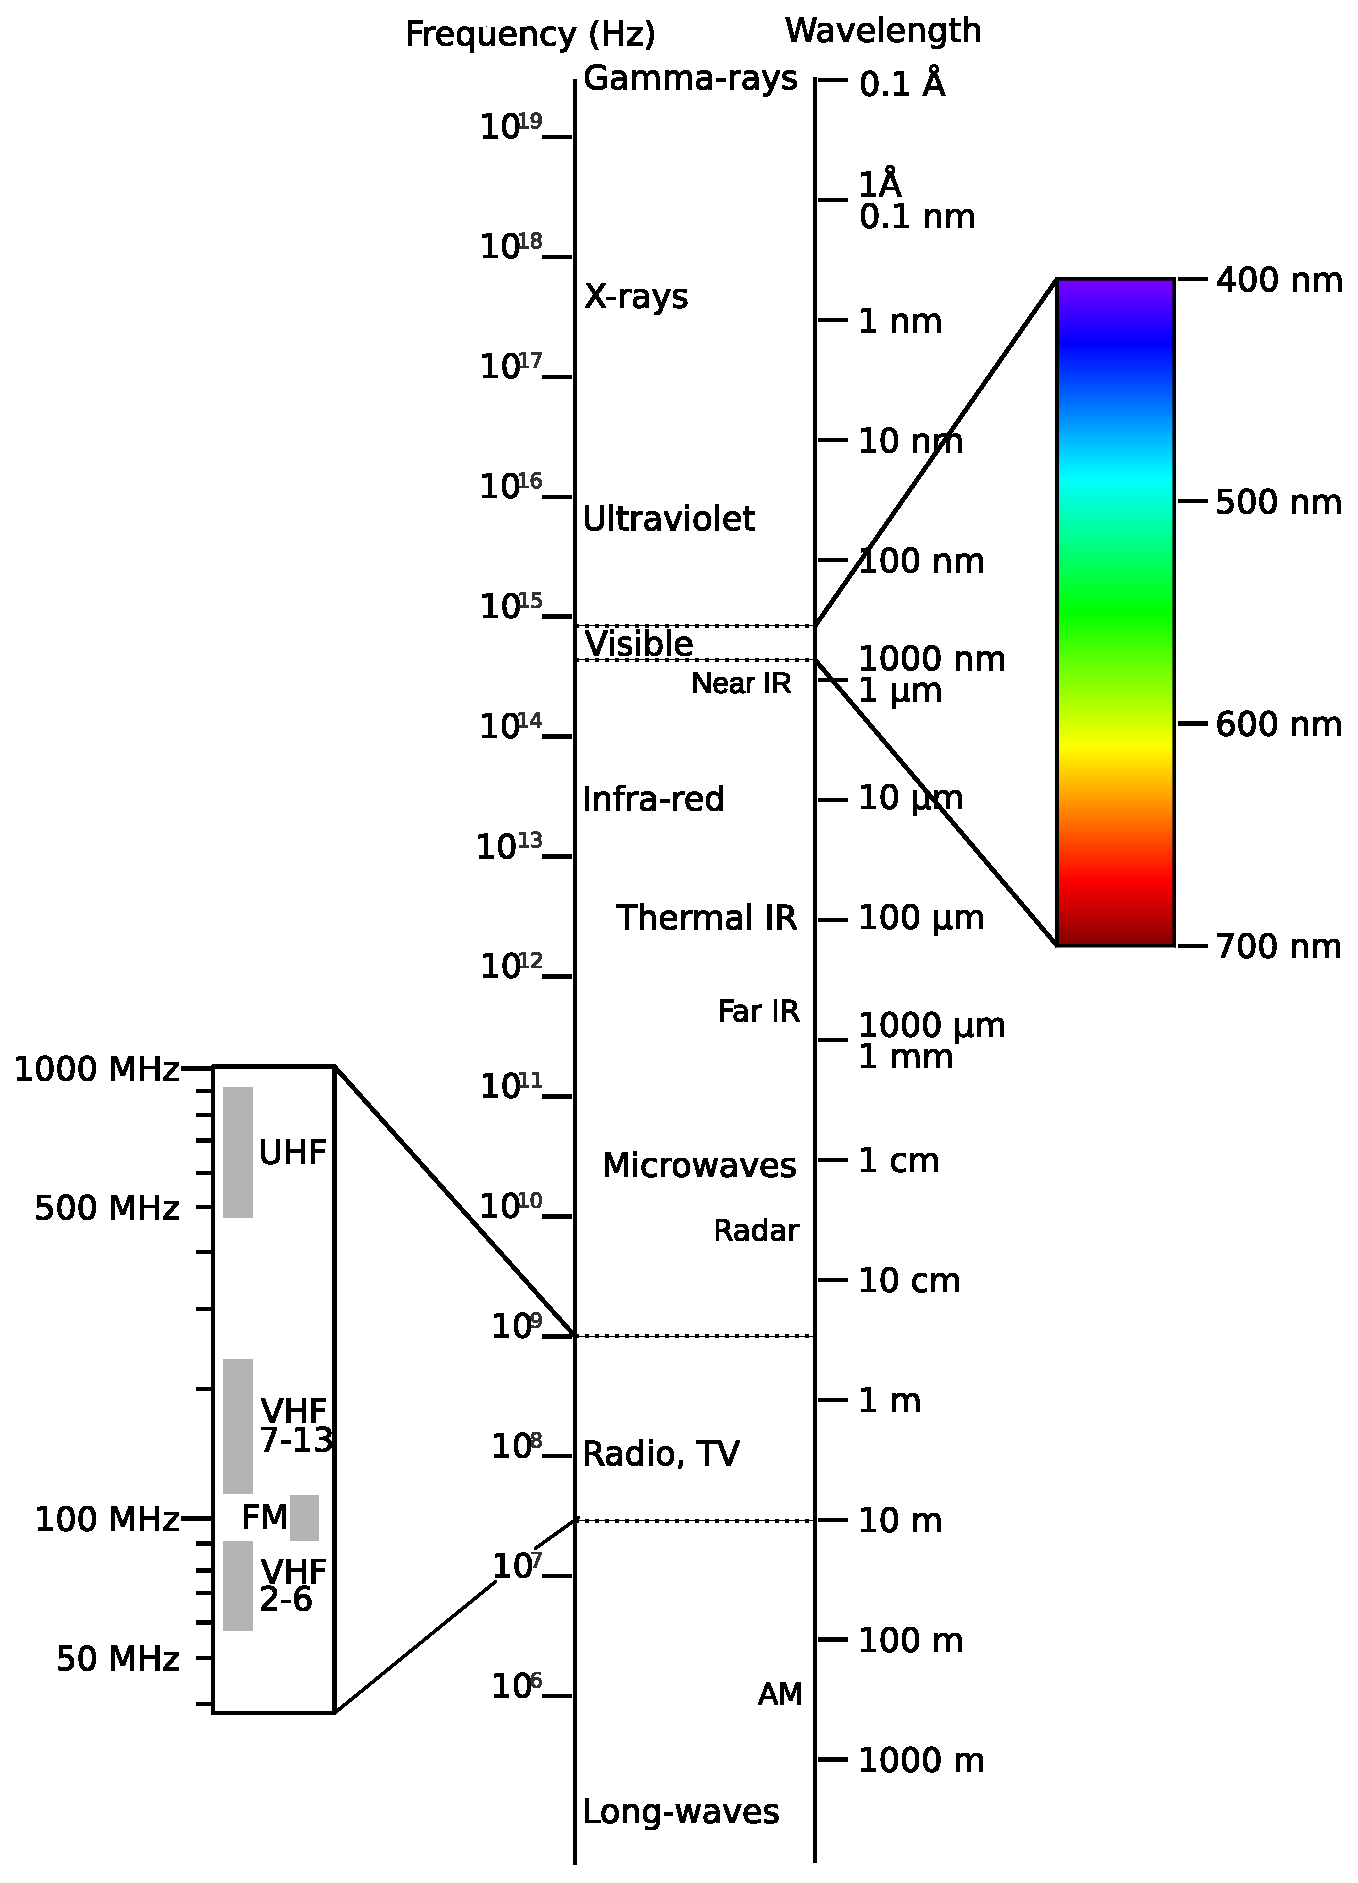
\includegraphics[width=\columnwidth]{modules/m0075_fEMS.eps}}}{A graphical depiction of the range of the electromagnetic spectrum in terms of frequency (10 raised to 6 to 10 raised to 19 Hz) and wavelength (1000 m to 0.01 nm). Shown as a tall rectangle, highlighted spectra are the radio spectrum (50 MHz to 1000 MHz from bottom to top) and the wavelengths in the optical band (700 nm to 400 nm from bottom to top).}
\end{center} 
%\vspace{2in}
% https://commons.wikimedia.org/wiki/File:Electromagnetic-Spectrum.svg
\centerline{\scriptsize 
\copyright~\hyperref[m0075_fEMS_Credit]{V.\ Blacus} 
\href{https://creativecommons.org/licenses/by-sa/3.0/}{CC BY-SA 3.0} 
} 
\caption{
\label{m0075_fEMS}
Electromagnetic Spectrum.
}
\end{figure}
%
\begin{table*}[t]
\begin{center}
\begin{tabular}{lccl}
Band & Frequencies & Wavelengths & Typical Applications \\
\hline
EHF & 30-300~GHz & 10--1~mm & 60~GHz WLAN, Point-to-point data links \\
SHF & 3--30~GHz & 10--1~cm & Terrestrial \& Satellite data links, Radar \\ 
UHF & 300--3000~MHz & 1--0.1~m & TV broadcasting, Cellular, WLAN \\
VHF & 30--300~MHz & 10--1~m & FM \& TV broadcasting, LMR \\ 
HF & 3--30~MHz & 100--10~m & Global terrestrial comm., CB Radio \\
MF & 300--3000~kHz & 1000--100~m & AM broadcasting \\
LF & 30--300~kHz & 10--1~km & Navigation, RFID \\
VLF & 3--30~kHz & 100--10~km & Navigation \\
\end{tabular}
\end{center}
\caption{The radio portion of the electromagnetic spectrum, according to a common scheme for naming ranges of radio frequencies. WLAN: Wireless local area network, LMR: Land mobile radio, RFID: Radio frequency identification.}
%\label{cIntro_fRFS}
\label{m0075_tRFS}
\end{table*}

Similarly, the optical band is partitioned into the familiar ``rainbow'' of red through violet, as shown in Figure~\ref{m0075_fEMS} and Table~\ref{m0075_tOptical}. Other portions of the spectrum are sometimes similarly subdivided in certain applications.
%
%\begin{table*}[t]
\begin{table}
%\vspace{3in}
\begin{center}
\begin{tabular}{lcc}
Band & Frequencies & Wavelengths \\
\hline
Violet & 668--789~THz & 450--380~nm  \\
Blue   & 606--668~THz & 495--450~nm  \\
Green  & 526--606~THz & 570--495~nm  \\ 
Yellow & 508--526~THz & 590--570~nm  \\
Orange & 484--508~THz & 620--590~nm  \\
Red    & 400--484~THz & 750--620~nm  \\
\end{tabular}
\end{center}
\caption{The optical portion of the electromagnetic spectrum.}
% https://en.wikipedia.org/wiki/Visible_spectrum 
\label{m0075_tOptical}
%\end{table*}
\end{table}

%%% https://commons.wikimedia.org/wiki/File:Atmospheric_electromagnetic_opacity.svg

{\bf Additional Reading:}
\begin{itemize}
\item ``\href{https://en.wikipedia.org/wiki/Electromagnetic_spectrum}{Electromagnetic spectrum}'' on Wikipedia.
\item ``\href{https://en.wikipedia.org/wiki/Photoelectric_effect}{Photoelectric effect}'' on Wikipedia.
\end{itemize}


      \vfill\break
    \section{Fundamentals of Waves}
{\color{blue}\tiny[m0074]}      % This is text associated with the open textbook "Open Electromagnetics"
% See immediately below for author, date
% <License info goes here (boilerplate, not read by project compiler)>

%ORB TITLE Fundamentals of Waves  
%ORB AUTHOR 0       # S.W. Ellingson, Virginia Tech (ellingson@vt.edu)
%ORB DATE   20180731
%ORB ABSTRACT 

\label{m0074_Fundamentals_of_Waves} % <-- Must match name of this file and module directory name.  Don't mess with this!
\index{waves!fundamentals|(}

In this section, we formally introduce the concept of a wave and explain some basic characteristics.

To begin, let us consider not electromagnetic waves, but rather sound waves.  
To be clear, sound waves 
\index{sound (waves)}
and electromagnetic waves are completely distinct phenomena. Sound waves are variations in pressure, whereas electromagnetic waves are variations in electric and magnetic fields.
However, the mathematics that govern sound waves and electromagnetic waves are very similar, so the analogy provides useful insight.
Furthermore, sound waves are intuitive for most people because they are readily observed.   
So, here we go:

Imagine standing in an open field and that it is completely quiet.
In this case, the air pressure everywhere is about 101~kPa (101,000 N/m$^2$) at sea level, % 101.325, https://en.wikipedia.org/wiki/Atmospheric_pressure
and we refer to this as the \emph{quiescent air pressure}.
Sound can be described as the \emph{differential air pressure} $p(x,y,z,t)$, which we define as the absolute air pressure at the spatial coordinates $(x,y,z)$ minus the quiescent air pressure. 
So, when there is no sound, $p(x,y,z,t)=0$.
The function $p$ as an example of a  \emph{scalar field}.\footnote{Although it's not important in this section, you can read about the concept of a ``field'' in Section~\ref{m0001_What_is_a_Field}.}
\index{field!scalar}
\index{scalar field|see {field, scalar}}

Let's also say you are standing at $x=y=z=0$ and you have brought along a friend who is standing at $x=d$; i.e., a distance $d$ from you along the $x$ axis.
Also, for simplicity, let us consider only what is happening along the $x$ axis; i.e., $p(x,t)$.

At $t=0$, you clap your hands once.
This forces the air between your hands to press outward, creating a region of increased pressure (i.e., $p>0$) that travels outward.  
As the region of increased pressure moves outward, it leaves behind a region of low pressure where $p<0$.
Air molecules immediately move toward this region of lower pressure, and so the air pressure quickly returns to the quiescent value, $p=0$.
The traveling disturbance in $p(x,t)$ is the sound of the clap.
The disturbance continues to travel outward until it reaches your friend, who then hears the clap. 

At each point in time, you can make a plot of $p(x,t)$ versus $x$ for the current value of $t$.
This is shown in Figure~\ref{m0074_fClap}.
At times $t<0$, we have simply $p(x,t)=0$.
A short time after $t=0$, the peak pressure is located at slightly to the right of $x=0$.
The pressure is not a simple impulse because interactions between air molecules constrain the pressure to be continuous over space.
So instead, we see a rounded pulse representing the rapid build-up and similarly rapid decline in air pressure.
A short time later $p(x,t)$ looks very similar, except the pulse is now further away.
%
\begin{figure}
\begin{center}
\pdftooltip{{  % note double braces
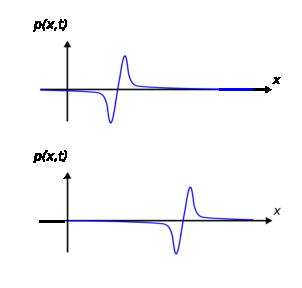
\includegraphics[width=2.5in]{modules/m0074_fClap.eps}
}}{The figure shows two x-y plots, one above the other. Differential pressure is on the y-axis and distance is on the x-axis. In each graph, the area of increased pressure is represented by one period of an approximately-sinusoidal waveform. The bottom graph shows the waveform farther away on the x-axis than the top graph.}
\end{center} 
%\vspace{2in}
% https://commons.wikimedia.org/wiki/File:M0074_fClap.svg
\centerline{\scriptsize 
\copyright~\hyperref[m0074_fClap_Credit]{Y.\ Qin} 
\href{https://creativecommons.org/licenses/by/4.0/}{CC BY 4.0} 
} 
\caption{
\label{m0074_fClap}
The differential pressure $p(x,t)$ (\emph{top}) a short time after the clap and (\emph{bottom}) a slightly longer time after the clap.
}
\end{figure}

Now: What precisely is $p(x,t)$?
% https://en.wikipedia.org/wiki/Acoustic_wave_equation
Completely skipping over the derivation, the answer is that $p(x,t)$ is the solution to the \emph{acoustic wave equation} 
\index{wave equation!acoustic}
\index{acoustic wave equation|see {wave equation, acoustic}}
(see ``Additional References'' at the end of this section):
%
\begin{equation}
\frac{\partial^2 p}{\partial x^2} - \frac{1}{c_s^2}\frac{\partial^2 p}{\partial t^2} = 0
\label{m0074_eAcousticWaveEquation}
\end{equation}
%
where $c_s$ is the speed of sound, which is about 340~m/s at sea level. % https://en.wikipedia.org/wiki/Speed_of_sound
Just to emphasize the quality of the analogy between sound waves and electromagnetic waves, know that the acoustic wave equation is mathematically identical to equations that that govern electromagnetic waves.

Although ``transient'' phenomena -- analogous to a clap -- are of interest in electromagnetics, an even more common case of interest is the wave resulting from a sinusoidally-varying source.  We can demonstrate this kind of wave in the context of sound as well.
Here we go: 

In the previous scenario, you pick up a trumpet and blow a perfect A note.
The A note is 440~Hz, meaning that the air pressure emerging from your trumpet is varying sinusoidally at a frequency of 440~Hz.
Let's say you can continue to blow this note long enough for the entire field to be filled with the sound of your trumpet.
Now what does the pressure-versus-distance curve look like?
Two simple observations will settle that question:
%
\begin{itemize}
\item $p(x,t)$ at any \emph{constant position} $x$ is a sinusoid as a function of $x$.  
This is because the acoustic wave equation is linear and time invariant, so a sinusoidal excitation (i.e., your trumpet) results in a sinusoidal response at the same frequency (i.e., the sound heard by your friend).
\item $p(x,t)$ at any \emph{constant time} $t$ is also a sinusoid as a function of $x$.
This is because the sound is propagating away from the trumpet and toward your friend, and anyone in between will also hear the A note, but with a phase shift determined by the difference in distances.
\end{itemize}
%
This is enough information to know that the solution must have the form:
%
\begin{equation}
p(x,t) = A_m \cos\left( \omega t - \beta x + \psi \right)
\label{m0074_eGenericWave}
\end{equation} 
%
where $\omega = 2\pi f$, $f=440$~Hz, and $A_m$, $\beta$, and $\psi$ remain to be determined.

You can readily verify that Equation~\ref{m0074_eGenericWave} satisfies the acoustic wave equation when
%
\begin{equation}
\beta = \frac{\omega}{c_s}
\end{equation}
%
In this problem, we find $\beta\cong 8.13$~rad/m. 
This means that at any given time, the difference in phase measured between any two points separated by a distance of 1~m is 8.13~rad.
The parameter $\beta$ goes by at least three names: \emph{phase propagation constant}, 
\index{propagation constant!phase}
\emph{wavenumber}, 
and \emph{spatial frequency}.
\index{spatial frequency}
The term ``spatial frequency'' is particularly apt, since $\beta$ plays precisely the same role for distance ($x$) as $\omega$ plays for time ($t$) -- This is apparent from Equation~\ref{m0074_eGenericWave}.
However, ``wavenumber'' is probably the more commonly-used term.

%ORB HIGHLIGHT
\begin{mdframed}[backgroundcolor=yellow!20,nobreak=true] 
The wavenumber 
\index{wavenumber}
$\beta$ (rad/m) is the rate at which the phase of a sinusoidal wave progresses with distance.   
\end{mdframed}

Note that $A_m$ and $\psi$ are not determined by the wave equation, but instead are properties of the source.
Specifically, $A_m$ is determined by how hard we blow, and $\psi$ is determined by the time at which we began to blow and the location of the trumpet.
For simplicity, let us assume that we begin to blow at time $t\ll 0$; i.e., in the distant past so that the sound pressure field has achieved steady state by $t=0$.
Also, let us set $\psi=0$ and set $A_m=1$ in whatever units we choose to express $p(x,t)$.
We then have:
%
\begin{equation}
p(x,t) = \cos\left( \omega t - \beta x \right)
\label{m0074_eSimpleWave}
\end{equation} 
%
Now we have everything we need to make plots of $p(x)$ at various times.

Figure~\ref{m0074_fTrumpet}(a) shows $p(x,t=0)$.
As expected, $p(x,t=0)$ is periodic in $x$.  
The associated period is referred to as the \emph{wavelength} $\lambda$.
Since $\lambda$ is the distance required for the phase of the wave to increase by $2\pi$~rad, and because phase is increasing at a rate of $\beta$ rad/m, we find:
%
\begin{equation}
\lambda = \frac{2\pi}{\beta}
\end{equation}
%
In the present example, we find $\lambda\cong 77.3$~cm.
%
\begin{figure}
\begin{center}
\pdftooltip{{  % note double braces
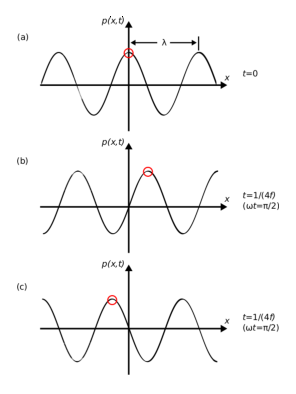
\includegraphics[width=2.9in]{modules/m0074_fTrumpet.eps}
}}{The figure shows three graphs: (a) is above (b) which is above (c). The three graphs have sinusoidal waves of identical wavelengths and amplitudes. In (a), a red circle pinpoints the peak of the wave which coincides with the y-intercept. In (b), this same peak is a quarter wavelength to the right of the y-axis. In (c), it is a quarter wavelength to the left of the y-axis.}
\end{center} 
%\vspace{2in}
% https://commons.wikimedia.org/wiki/File:M0074_fTrumpet.svg
\centerline{\scriptsize 
\copyright~\hyperref[m0074_fTrumpet_Credit]{Y.\ Qin} 
\href{https://creativecommons.org/licenses/by/4.0/}{CC BY 4.0} 
} 
\caption{
\label{m0074_fTrumpet}
The differential pressure $p(x,t)$ for 
(a) $t=0$,
(b) $t=1/4f$ for ``$-\beta x$,'' as indicated in Equation~\ref{m0074_eSimpleWave} (wave traveling to right); and
(c) $t=1/4f$ for ``$+\beta x$'' (wave traveling to left).
}
\end{figure}

%ORB HIGHLIGHT
\begin{mdframed}[backgroundcolor=yellow!20,nobreak=true]
Wavelength 
\index{wavelength}
$\lambda=2\pi/\beta$ is the distance required for the phase of a sinusoidal wave to increase by one complete cycle (i.e., $2\pi$ rad) at any given time. 
\end{mdframed}

Now let us consider the situation at $t=+1/4f$, which is $t=568~\mu$s and $\omega t=\pi/2$.
We see in Figure~\ref{m0074_fTrumpet}(b) that the waveform has shifted a distance $\lambda/4$ to the right.
It is in this sense that we say the wave is propagating in the $+x$ direction.
Furthermore, we can now compute a \emph{phase velocity} $v_p$: 
We see that a point of constant phase has shifted a distance $\lambda/4$ in time $1/4f$, so   
%
\begin{equation}
v_p = \lambda f 
\end{equation}
%
In the present example, we find $v_p\cong 340$~m/s; i.e., we have found that the phase velocity is equal to the speed of sound $c_s$.  
It is in this sense that we say that the phase velocity is the speed at which the wave propagates.\footnote{It is worth noting here is that ``velocity'' is technically a vector; i.e., speed in a given direction. Nevertheless, this quantity is actually just a speed, and this particular abuse of terminology is generally accepted.}

%ORB HIGHLIGHT
\begin{mdframed}[backgroundcolor=yellow!20,nobreak=true]
Phase velocity 
\index{phase velocity}
$v_p=\lambda f$ is the speed at which a point of constant phase in a sinusoidal waveform travels.  
\end{mdframed}

Recall that in Equation~\ref{m0074_eGenericWave} we declared that $\beta x$ is subtracted from the argument of the sinusoidal function.  
To understand why, let's change the sign of $\beta x$ and see if it still satisfies the wave equation -- one finds that it does.
Next, we repeat the previous experiment and see what happens.
The result is shown in Figure~\ref{m0074_fTrumpet}(c).
Note that points of constant phase have traveled an equal distance, but now in the $-x$ direction.  
In other words, this alternative choice of sign for $\beta x$ within the argument of the cosine function represents a wave that is propagating in the opposite direction.  
This leads us to the following realization:

%ORB HIGHLIGHT
\begin{mdframed}[backgroundcolor=yellow!20,nobreak=true]
If the phase of the wave is decreasing with $\beta x$, then the wave is propagating in the $+x$ direction.
If the phase of the wave is increasing with $\beta x$, then the wave is propagating in the $-x$ direction.
\end{mdframed}

Since the prospect of sound traveling toward the trumpet is clearly nonsense in the present situation, we may neglect the latter possibility.
However, what happens if there is a wall located in the distance, behind your friend?
Then, we expect an echo from the wall, which would be a second wave propagating in the reverse direction and for which the argument of the cosine function would contain the term ``$+\beta x$.''

Finally, let us return to electromagnetics.  
Electromagnetic waves satisfy precisely the same wave equation (i.e., Equation~\ref{m0074_eAcousticWaveEquation}) as do sound waves, except that the phase velocity is much greater.
Interestingly, though, the frequencies of electromagnetic waves are also much greater than those of sound waves, so we can end up with wavelengths having similar orders of magnitude.
In particular, an electromagnetic wave with $\lambda=77.3$~cm (the wavelength of the ``A'' note in the preceding example) lies in the radio portion of the electromagnetic spectrum.

An important difference between sound and electromagnetic waves is that electromagnetic waves are vectors; that is, they have \emph{direction} as well as magnitude.
Furthermore, we often need to consider multiple electromagnetic vector waves (in particular, both the \emph{electric field} and the \emph{magnetic field}) in order to completely understand the situation.
Nevertheless the concepts of wavenumber, wavelength, phase velocity, and direction of propagation apply in precisely the same manner to electromagnetic waves as they do to sound waves.  

{\bf Additional Reading:}
\begin{itemize}
\item ``\href{https://en.wikipedia.org/wiki/Wave_equation}{Wave Equation}'' on Wikipedia.
\item ``\href{https://en.wikipedia.org/wiki/Acoustic_wave_equation}{Acoustic Wave Equation}'' on Wikipedia.
\end{itemize}

\index{waves!fundamentals|)}













      \vfill\break
    \section{Guided and Unguided Waves}
{\color{blue}\tiny[m0040]}      % This is text associated with the open textbook "Open Electromagnetics"
% See immediately below for author, date
% <License info goes here (boilerplate, not read by project compiler)>

%ORB TITLE Guided and Unguided Waves  
%ORB AUTHOR 0       # S.W. Ellingson, Virginia Tech (ellingson@vt.edu)
%ORB DATE   20180730
%ORB ABSTRACT Guided and Unguided Waves  

\label{m0040_Guided_vs_Unguided_Waves} % <-- Must match name of this file and module directory name.  Don't mess with this!

Broadly speaking, waves may be either \emph{guided} or \emph{unguided}.

Unguided waves include those that are radiated by antennas, as well as those that are unintentionally radiated.
Once initiated, these waves propagate in an uncontrolled manner until they are redirected by scattering or dissipated by losses associated with materials.

Examples of guided waves are those that exist within structures such as transmission lines, waveguides, and optical fibers.  We refer to these as guided because they are constrained to follow the path defined by the structure.

%ORB HIGHLIGHT
\begin{mdframed}[backgroundcolor=yellow!20,nobreak=true]
Antennas and unintentional radiators emit \emph{unguided waves}.
\index{waves!unguided}
Transmission lines, waveguides, and optical fibers carry \emph{guided waves}. 
\index{waves!guided}
\end{mdframed}


      \vfill\break
    \section{Phasors}
{\color{blue}\tiny[m0033]}      % This is text associated with the open textbook "Open Electromagnetics"
% See immediately below for author, date
% <License info goes here (boilerplate, not read by project compiler)>

%ORB TITLE Phasors
%ORB AUTHOR 0        # S.W. Ellingson, Virginia Tech (ellingson@vt.edu)
%ORB DATE 20180814   # yyyymmdd
%ORB ABSTRACT Phasors: Basic concepts, conversion to and from time-domain, properties, comments on applicability

\label{m0033_Phasors} % <-- Must match name of this file and module directory name.  Don't mess with this!
\index{phasor|(}

In many areas of engineering, signals are well-modeled as sinusoids.
Also, devices that process these signals are often well-modeled as linear time-invariant (LTI) systems.
The response of an LTI system to any linear combination of sinusoids is another linear combination of sinusoids having the same frequencies.\footnote{ A ``linear combination'' of functions $f_i(t)$ where $i=1,2,3,...$ is $\sum_i {a_i f_i(t)}$ where the $a_i$'s are constants.}
In other words, 
(1) sinusoidal signals processed by LTI systems remain sinusoids and are not somehow transformed into square waves or some other waveform; and 
(2) we may calculate the response of the system for one sinusoid at a time, and then add the results to find the response of the system when multiple sinusoids are applied simultaneously.
This property of LTI systems is known as \emph{superposition}.
\index{superposition}

The analysis of systems that process sinusoidal waveforms is greatly simplified when the sinusoids are represented as \emph{phasors}.
Here is the key idea:
%
%ORB HIGHLIGHT
\begin{mdframed}[backgroundcolor=yellow!20,nobreak=true] 
A \emph{phasor} 
\index{phasor (definition)}
is a complex-valued number that represents a real-valued sinusoidal waveform.  Specifically, a phasor has the magnitude and phase of the sinusoid it represents.
\end{mdframed}

Figures~\ref{m0033_fComplexPlane} and \ref{m0033_fSinusoids} show some examples of phasors and the associated sinusoids.  
%
\begin{figure}
\begin{center}
\pdftooltip{{  % note double braces
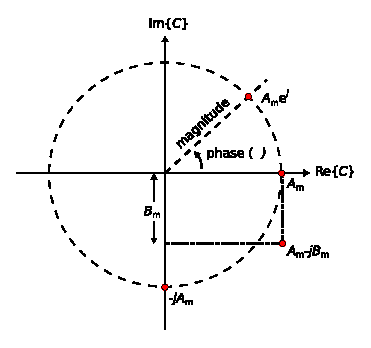
\includegraphics[width=3in]{modules/m0033_fComplexPlane.eps}
}}{A dotted circle is plotted on an imaginary versus real plane with the origin as its center. A rectangle is superimposed on the plane with vertices at (0, 0), (0, -j B sub m), (A sub m, 0) and (A sub m, -j B sub m)  B sub m is the distance along the negative imaginary axis. A sub m is the distance along the positive real axis and is equal to the radius of the circle. In the positive real quadrant, magnitude is labeled as an line running from the origin to the circle at a phase angle of psi. The magnitude line intersects at the point A sub m * e raised to the quantity i * psi.}
\end{center} 
%\vspace{3in}
\caption{\label{m0033_fComplexPlane} Examples of phasors, displayed here as points in the real-imaginary plane.
}
\end{figure}
%
\begin{figure}
\begin{center}
\pdftooltip{{  % note double braces
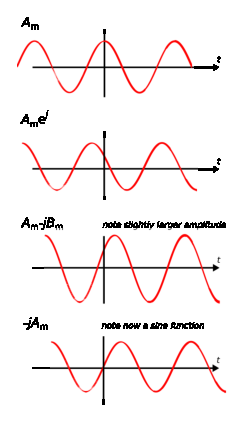
\includegraphics[width=2.5in]{modules/m0033_fSinusoids.eps}
}}{The figure shows four graphs in a column, each featuring sinusoidal waves with the x-axis labeled t. The top is labeled A sub m, and the middle wave, maximum amplitude intersects on the y-axis. The second is labeled A sub m * e raised to the quantity of j psi, and the middle wave maximum amplitude is slightly to the left of the y-axis. The third is labeled A sub m * quantity of -j B sub m, and has a slightly larger amplitude than the first or second with the middle wave maximum amplitude slightly to the right. The fourth is labeled -j * A sub m, and the midpoint intersects the origin.}
\end{center} 
\caption{\label{m0033_fSinusoids} Sinusoids corresponding to the phasors shown in Figure~\ref{m0033_fComplexPlane}.}
\end{figure}

It is important to note that a phasor by itself is not the signal.  
A phasor is merely a simplified mathematical representation in which the actual, real-valued physical signal is represented as a complex-valued constant. 

Here is a completely general form for a physical (hence, real-valued) quantity varying sinusoidally with angular frequency $\omega=2\pi f$:
%
\begin{equation}
A(t;\omega) = A_m(\omega) \cos{(\omega t + \psi(\omega))}
\end{equation} 
%
where 
$A_m(\omega)$ is magnitude at the specified frequency, 
$\psi(\omega)$ is phase at the specified frequency, 
and $t$ is time.  
Also, we require $\partial A_m/\partial t =0$; that is, that the time variation of $A(t)$ is completely represented by the cosine function alone. 
Now we can equivalently express $A(t;\omega)$ as a phasor $C(\omega)$:
%
\begin{equation}
C(\omega) = A_m(\omega) e^{j\psi(\omega)}
\label{m0033_eCOmega}
\end{equation}
%
To convert this phasor back to the physical signal it represents, we (1) restore the time dependence by multiplying by $e^{j\omega t}$, and then (2) take the real part of the result.  In mathematical notation: 
%
%ORB HIGHLIGHT
\begin{mdframed}[backgroundcolor=yellow!20,nobreak=true] 
\begin{equation}
A(t;\omega) = \mbox{R{e}} \left\{ C(\omega) e^{j\omega t} \right\}
\label{m0033_ePhasor}
\end{equation} 
\end{mdframed}
%
To see why this works, simply substitute the right hand side of Equation~\ref{m0033_eCOmega} into Equation~\ref{m0033_ePhasor}.  Then:
\begin{equation}
\begin{split}
A(t) & = \mbox{Re}\left\{ A_m(\omega) e^{j\psi(\omega)} e^{j\omega t} \right\} \\
    ~& = \mbox{Re}\left\{ A_m(\omega) e^{j\left(\omega t + \psi(\omega)\right)} \right\} \\
    ~& = \mbox{Re}\left\{ A_m(\omega) \left[   \cos\left(\omega t + \psi(\omega)\right)  \right. \right. \\
    ~& ~~~~~~~~~~~~~~~ \left.              \left. +j\sin\left(\omega t + \psi(\omega)\right)  \right] \right\} \\
    ~& = A_m(\omega) \cos\left(\omega t + \psi(\omega)\right) 
\end{split}
\nonumber
\end{equation}
%
as expected.

It is common to write Equation~\ref{m0033_eCOmega} as follows, dropping the explicit indication of frequency dependence:
%
\begin{equation}
C = A_m e^{j\psi}
\end{equation}
%
This does not normally cause any confusion since the definition of a phasor requires that values of $C$ and $\psi$ are those that apply at whatever frequency is represented by the suppressed sinusoidal dependence $e^{j\omega t}$.   

Table~\ref{m0033_tPhasorExamples} shows mathematical representations of the same phasors demonstrated in Figure~\ref{m0033_fComplexPlane} (and their associated sinusoidal waveforms in Figure~\ref{m0033_fSinusoids}).
It is a good exercise is to confirm each row in the table, transforming from left to right and vice-versa.
%
\begin{table*}[t]
\begin{center}
\begin{tabular}{ll|l}
$A(t)$ & ~ & $C$ \\
\hline
$A_m \cos \left( \omega t \right)$ & ~ & $A_m$ \\
$A_m \cos \left( \omega t + \psi \right)$ & ~ & $A_m e^{j\psi}$ \\  
$A_m \sin \left( \omega t \right)$ & $= A_m \cos \left( \omega t - \frac{\pi}{2}\right)$ & $-jA_m$ \\  
$A_m \cos \left( \omega t \right) + B_m \sin \left( \omega t \right)$ & $= A_m \cos \left( \omega t \right) + B_m \cos \left( \omega t - \frac{\pi}{2}\right)$ & $A_m-jB_m$ \\  
\end{tabular}
\end{center}
\caption{\label{m0033_tPhasorExamples}Some examples of physical (real-valued) sinusoidal signals and the corresponding phasors. $A_m$ and $B_m$ are real-valued and constant with respect to $t$. 
}
\end{table*}

It is not necessary to use a phasor to represent a sinusoidal signal.  
We choose to do so because phasor representation leads to dramatic simplifications.
For example:
%  
\begin{itemize}
\item Calculation of the peak value from data representing $A(t;\omega)$ requires a time-domain search over one period of the sinusoid. However, if you know $C$, the peak value of $A(t)$ is simply $\left|C\right|$, and no search is required.
\item Calculation of $\psi$ from data representing $A(t;\omega)$ requires correlation (essentially, integration) over one period of the sinusoid. However, if you know $C$, then $\psi$ is simply the phase of $C$, and no integration is required.
\end{itemize}
%
Furthermore, mathematical operations applied to $A(t;\omega)$ can be equivalently performed as operations on $C$, and the latter are typically much easier than the former. 
To demonstrate this, we first make two important claims and show that they are true.

\rule{3in}{1pt}\\~\\

{\bf Claim 1}: Let $C_1$ and $C_2$ be two complex-valued constants (independent of $t$).  Also,  $\mbox{Re} \left\{ C_1 e^{j\omega t} \right\} = \mbox{Re} \left\{ C_2 e^{j\omega t} \right\}$ for all $t$.  Then, $C_1=C_2$. 

{\it Proof:} Evaluating at $t=0$ we find $\mbox{Re} \left\{ C_1 \right\} = \mbox{Re} \left\{ C_2 \right\}$.  Since $C_1$ and $C_2$ are constant with respect to time, this must be true for all $t$.  At $t=\pi/(2\omega)$ we find
%
\begin{equation}
\mbox{R{e}} \left\{ C_1 e^{j\omega t} \right\} = \mbox{R{e}} \left\{ C_1 \cdot j \right\} = -\mbox{Im} \left\{ C_1 \right\}
\nonumber
\end{equation}
%
and similarly
%
\begin{equation}
\mbox{R{e}} \left\{ C_2 e^{j\omega t} \right\} = \mbox{R{e}} \left\{ C_2 \cdot j \right\} = -\mbox{Im} \left\{ C_2 \right\}
\nonumber
\end{equation}
%
therefore $\mbox{Im} \left\{ C_1 \right\} = \mbox{Im} \left\{ C_2 \right\}$. Once again: Since $C_1$ and $C_2$ are constant with respect to time, this must be true for all $t$.  Since the real and imaginary parts of $C_1$ and $C_2$ are equal, $C_1 = C_2$. 

{\it What does this mean?} We have just shown that if two phasors are equal, then the sinusoidal waveforms that they represent are also equal. 

\rule{3in}{1pt}\\~\\

{\bf Claim 2}:  For any real-valued linear operator $\mathcal{T}$ and complex-valued quantity $C$, $\mathcal{T}( \mbox{Re}\left\{ C \right\} ) = \mbox{Re}\left\{ \mathcal{T}(C) \right\}$.

{\it Proof:} Let $C = c_r + jc_i$ where $c_r$ and $c_i$ are real-valued quantities, and evaluate the right side of the equation:
%
\begin{equation}
\begin{split}
\mbox{Re}\left\{ \mathcal{T}(C) \right\}& = \mbox{Re}\left\{ \mathcal{T}(c_r + jc_i) \right\} \\
                                       ~& = \mbox{Re}\left\{ \mathcal{T}(c_r) + j\mathcal{T}(c_i) \right\} \\
                                       ~& = \mathcal{T}(c_r) \\
                                       ~& = \mathcal{T}( \mbox{Re}\left\{ C \right\} )
\end{split}
\nonumber
\end{equation}

\emph{What does this mean?} 
The operators that we have in mind for $\mathcal{T}$ include addition, multiplication by a constant, differentiation, integration, and so on.  
Here's an example with differentiation:
%
\begin{equation}
\mbox{Re}\left\{ \frac{\partial}{\partial \omega} C \right\}  
= \mbox{Re}\left\{ \frac{\partial}{\partial \omega} (c_r + jc_i) \right\} 
= \frac{\partial}{\partial \omega} c_r
\nonumber
\end{equation}
%
\begin{equation}
\frac{\partial}{\partial \omega} \mbox{Re}\left\{ C \right\}  
= \frac{\partial}{\partial \omega} \mbox{Re}\left\{ (c_r + jc_i) \right\} 
= \frac{\partial}{\partial \omega} c_r
\nonumber
\end{equation}
%
In other words, differentiation of a sinusoidal signal can be accomplished by differentiating the associated phasor, so there is no need to transform a phasor back into its associated real-valued signal in order to perform this operation.

\rule{3in}{1pt}
      
\vfill\break %%%

Summarizing:
%
%ORB HIGHLIGHT
\begin{mdframed}[backgroundcolor=yellow!20,nobreak=true] 
Claims~1 and 2 together entitle us to perform operations on phasors as surrogates for the physical, real-valued, sinusoidal waveforms they represent.  Once we are done, we can transform the resulting phasor back into the physical waveform it represents using Equation~\ref{m0033_ePhasor}, if desired.
\end{mdframed}
%
However, a final transformation back to the time domain is usually \emph{not} desired, since the phasor tells us everything we can know about the corresponding sinusoid.

A skeptical student might question the value of phasor analysis on the basis that signals of practical interest are sometimes not sinusoidally-varying, and therefore phasor analysis seems not to apply generally.  
It is certainly true that many signals of practical interest are not sinusoidal, and many are far from it.  
Nevertheless, phasor analysis \emph{is} broadly applicable.  There are basically two reasons why this is so:
%
\begin{itemize}
\item 
Many signals, although not strictly sinusoidal, are ``narrowband'' and therefore well-modeled as sinusoidal. 
For example,  a cellular telecommunications signal might have a bandwidth on the order of 10~MHz and a center frequency of about 2~GHz.  
This means the difference in frequency between the band edges of this signal is just 0.5\% of the center frequency.  
The frequency response associated with signal propagation or with hardware can often be assumed to be constant over this range of frequencies.   
With some caveats, doing phasor analysis at the center frequency and assuming the results apply equally well over the bandwidth of interest is often a pretty good approximation.
\item 
It turns out that phasor analysis is easily extensible to any physical signal, regardless of bandwidth.  
This is so because any physical signal can be decomposed into a linear combination of sinusoids -- this is known as \emph{Fourier analysis}. 
The way to find this linear combination of sinusoids is by computing the \emph{Fourier series}, 
\index{Fourier series}
if the signal is periodic, or the \emph{Fourier Transform}, 
\index{Fourier transform}
otherwise.
Phasor analysis applies to each frequency independently, and (invoking superposition) the results can be added together to obtain the result for the complete signal.
The process of combining results after phasor analysis results is nothing more than integration over frequency; i.e.:
%
\begin{equation}
\int_{-\infty}^{+\infty} A(t;\omega) d\omega 
\nonumber
\end{equation}
%
Using Equation~\ref{m0033_ePhasor}, this can be rewritten:
%
\begin{equation}
\int_{-\infty}^{+\infty} \mbox{R{e}} \left\{ C(\omega) e^{j\omega t} \right\} d\omega
\nonumber
\end{equation}
%
We can go one step further using Claim~2:
 %
\begin{equation}
\mbox{R{e}} \left\{  \int_{-\infty}^{+\infty} C(\omega) e^{j\omega t} d\omega \right\} 
\nonumber
\end{equation} 
%
The quantity in the curly braces is simply the Fourier transform of $C(\omega)$.   
Thus, we see that we can analyze a signal of arbitrarily-large bandwidth simply by keeping $\omega$ as an independent variable while we are doing phasor analysis, and if we ever need the physical signal, we just take the real part of the Fourier transform of the phasor.
So not only is it possible to analyze any time-domain signal using phasor analysis, it is also often far easier than doing the same analysis on the time-domain signal directly.
\end{itemize}

\vfill\break %%%

Summarizing:
%ORB HIGHLIGHT
\begin{mdframed}[backgroundcolor=yellow!20,nobreak=true] 
Phasor analysis does not limit us to sinusoidal waveforms. Phasor analysis is not only applicable to sinusoids and signals that are sufficiently narrowband, but is also applicable to signals of arbitrary bandwidth via Fourier analysis.
\end{mdframed}

%%%%%%%%%%%%%%%%%%%%%%%%%%%%%%%%%%%%

{\bf Additional Reading:}
\begin{itemize}
\item ``\href{https://en.wikipedia.org/wiki/Phasor}{Phasor}'' on Wikipedia.
\item ``\href{https://en.wikipedia.org/wiki/Fourier_analysis}{Fourier analysis}'' on Wikipedia.
\end{itemize}

\index{phasor|)}


      \vfill\break
    \section{Units}
{\color{blue}\tiny[m0072]}      % This is text associated with the open textbook "Open Electromagnetics"
% See immediately below for author, date
% <License info goes here (boilerplate, not read by project compiler)>

%ORB TITLE Units     
%ORB AUTHOR 0       # S.W. Ellingson, Virginia Tech (ellingson@vt.edu)
%ORB DATE   20180602
%ORB ABSTRACT SI system of units, prefixes (i.e., "kilo-", "milli-" etc), ref to 

\label{m0072_Units} % <-- Must match name of this file and module directory name.  Don't mess with this!
\index{units|(}

The term ``unit'' refers to the measure used to express a physical quantity.
For example, the mean radius of the Earth is about 6,371,000~meters; in this case the unit is the meter.

A number like ``6,371,000'' becomes a bit cumbersome to write, so it is common to use a prefix to modify the unit.
For example, the radius of the Earth is more commonly said to be 6371~kilometers, where one kilometer is understood to mean 1000~meters. 
It is common practice to use prefixes, such as ``kilo-,'' that yield values in the range $0.001$ to $10,000$.  
A list of standard prefixes appears in Table~\ref{m0072_tPrefix}.
%
\begin{table}[b!]
\begin{center}
\begin{tabular}{lll}
Prefix & Abbreviation & Multiply by: \\
\hline
exa & E & $10^{18}$ \\
peta & P & $10^{15}$ \\
tera & T & $10^{12}$ \\
giga & G & $10^{9}$ \\
mega & M & $10^{6}$ \\
kilo & k & $10^{3}$ \\
milli & m & $10^{-3}$ \\
micro & $\mu$ & $10^{-6}$ \\
nano & n & $10^{-9}$ \\
pico & p & $10^{-12}$ \\
femto & f & $10^{-15}$ \\
atto & a & $10^{-18}$ \\
\end{tabular}
\end{center}
\caption{Prefixes used to modify units.}
\label{m0072_tPrefix}
\end{table}

Writing out the names of units can also become tedious.
For this reason, it is common to use standard abbreviations; e.g., ``6731~km'' as opposed to ``6371~kilometers,'' where ``k'' is the standard abbreviation for the prefix ``kilo'' and ``m'' is the standard abbreviation for ``meter.''
A list of commonly-used base units and their abbreviations are shown in Table~\ref{m0072_tUnits}.
%
\begin{table}
\begin{center}
\begin{tabular}{lll}
Unit & Abbreviation & Quantifies: \\
\hline
ampere & A & electric current \\
coulomb & C & electric charge\\
farad & F & capacitance \\
henry & H & inductance \\
hertz & Hz & frequency\\
joule & J & energy \\
meter & m & distance \\
newton & N & force \\
ohm & $\Omega$ & resistance\\
second & s & time\\
tesla & T & magnetic flux density \\
volt & V & electric potential\\
watt & W & power\\
weber & Wb & magnetic flux \\
\end{tabular}
\end{center}
\caption{Some units that are commonly used in electromagnetics.  
}
\label{m0072_tUnits}
\end{table}

To avoid ambiguity, it is important to always indicate the units of a quantity; e.g., writing ``6371~km'' as opposed to ``6371.''
Failure to do so is a common source of error and misunderstandings.  
An example is the expression: 
$$l = 3t$$ 
where $l$ is length and $t$ is time.  It could be that $l$ is in meters and $t$ is in seconds, in which case ``$3$'' really means ``3~m/s''.
However, if it is intended that $l$ is in kilometers and $t$ is in hours, then ``$3$'' really means ``3~km/h'' and the equation is literally different.
To patch this up, one might write ``$l = 3t$~m/s''; however, note that this does does not resolve the ambiguity we just identified -- i.e., we still don't know the units of the constant ``3.''
Alternatively, one might write ``$l=3t$ where $l$ is in meters and $t$ is in seconds,'' which is unambiguous but becomes quite awkward for more complicated expressions.
A better solution is to write instead:
$$l = \left(3~\mbox{m/s}\right)t$$
or even better:
$$l = at ~~~\mbox{where $a=3$~m/s}$$
since this separates this issue of units from the perhaps more-important fact that $l$ is proportional to $t$ and the constant of proportionality ($a$) is known.

The meter is the fundamental unit of length in the International System of Units, known by its French acronym ``SI'' 
\index{SI (system of units)}
and sometimes informally referred to as the ``metric system.''  
\index{metric system}

%ORB HIGHLIGHT
\begin{mdframed}[backgroundcolor=yellow!20,nobreak=true] 
In this work, we will use SI units exclusively.
\end{mdframed}

Although SI is probably the most popular for engineering use overall, other systems remain in common use.  
For example, the English system, 
\index{English system of units}
where the radius of the Earth might alternatively be said to be about 3959~miles, continues to be used in various applications and to a lesser or greater extent in various regions of the world.
An alternative system in common use in physics and material science applications is the CGS
\index{CGS (system of units)}
(``centimeter-gram-second'') system. The CGS system is similar to SI, but with some significant differences. For example, the base unit of energy is the CGS system is not the ``joule'' but rather the ``erg,'' and the values of some physical constants become unitless. Therefore -- once again -- it is very important to include units whenever values are stated.

SI defines seven fundamental units from which all other units can be derived.  These fundamental units are
distance in meters (m),
time in seconds (s), 
current in amperes (A),
mass in kilograms (kg),
temperature in kelvin (K),
particle count in moles (mol), and
luminosity in candela (cd).
SI units for electromagnetic quantities such as coulombs (C) for charge and volts (V) for electric potential are derived from these fundamental units.

A frequently-overlooked feature of units is their ability to assist in error-checking mathematical expressions.
For example, the electric field intensity may be specified in volts per meter (V/m), so an expression for the electric field intensity that yields units of V/m is said to be ``dimensionally correct'' (but not necessarily correct), whereas an expression that cannot be reduced to units of V/m \emph{cannot} be correct. 

%%%%%%%%%%%%%%%%%%%%%%%%%%%%%%%%%%%%

{\bf Additional Reading:}
\begin{itemize}
\item ``\href{https://en.wikipedia.org/wiki/International_System_of_Units}{International System of Units}'' on Wikipedia.
\index{SI (system of units)}
\item ``\href{https://en.wikipedia.org/wiki/Centimetre-gram-second_system_of_units}{Centimetre-gram-second system of units}'' on Wikipedia.
\index{CGS (system of units)}
\end{itemize}

\index{units|)}

      \vfill\break
    \section{Notation}
{\color{blue}\tiny[m0005]}      % This is text associated with the open textbook "Open Electromagnetics"
% See immediately below for author, date
% <License info goes here (boilerplate, not read by project compiler)>

%ORB TITLE Notation
%ORB AUTHOR 0    # S.W. Ellingson, Virginia Tech (ellingson@vt.edu)
%ORB DATE 20180731  # yyyymmdd
%ORB ABSTRACT Explanation of notation; e.g., boldface means vector, tilde means phasor, carat means unit vector, etc. 

\label{m0005_Notation} % <-- Must match name of this file and module directory name.  Don't mess with this!
\index{notation|(}

The list below describes notation used in this book. 
%
\begin{itemize}
\item \emph{Vectors}: Boldface is used to indicate a vector; e.g., the electric field intensity vector will typically appear as ${\bf E}$.  Quantities not in boldface are scalars.  When writing by hand, it is common to write ``$\overline{E}$'' or ``$\overrightarrow{E}$'' in lieu of ``${\bf E}$.''
\item \emph{Unit vectors}: A circumflex is used to indicate a unit vector; i.e., a vector having magnitude equal to one.  For example, the unit vector pointing in the $+x$ direction will be indicated as $\hat{\bf x}$.  In discussion, the quantity ``$\hat{\bf x}$'' is typically spoken ``$x$ hat.'' 
\item \emph{Time}: The symbol $t$ is used to indicate time. 
\item \emph{Position}: The symbols $(x,y,z)$, $(\rho,\phi,z)$, and $(r,\theta,\phi)$ indicate positions using the Cartesian, cylindrical, and polar coordinate systems, respectively.  It is sometimes convenient to express position in a manner which is independent of a coordinate system; in this case, we typically use the symbol ${\bf r}$. For example, ${\bf r}=\hat{\bf x}x+\hat{\bf y}y+\hat{\bf z}z$ in the Cartesian coordinate system.
\item \emph{Phasors:}  A tilde is used to indicate a phasor quantity; e.g., a voltage phasor might be indicated as $\widetilde{V}$, and the phasor representation of ${\bf E}$ will be indicated as $\widetilde{{\bf E}}$.
\item \emph{Curves, surfaces, and volumes:} These geometrical entities will usually be indicated in script; e.g., an open surface might be indicated as $\mathcal{S}$ and the curve bounding this surface might be indicated as $\mathcal{C}$.  Similarly, the volume enclosed by a closed surface $\mathcal{S}$ may be indicated as $\mathcal{V}$.
\item \emph{Integrations over curves, surfaces, and volumes} will usually be indicated using a single integral sign with the appropriate subscript. For example:
$$ \int_{\mathcal{C}} \cdot\cdot\cdot ~dl ~~~~ \mbox{is an integral over the curve $\mathcal{C}$}$$
$$ \int_{\mathcal{S}} \cdot\cdot\cdot ~ds ~~~~ \mbox{is an integral over the surface $\mathcal{S}$}$$  
$$ \int_{\mathcal{V}} \cdot\cdot\cdot ~dv ~~~~ \mbox{is an integral over the volume $\mathcal{V}$.}$$ 
\item \emph{Integrations over \underline{closed} curves and surfaces} will be indicated using a circle superimposed on the integral sign. For example: 
$$ \oint_{\mathcal{C}} \cdot\cdot\cdot ~dl ~~~~ \mbox{is an integral over the closed curve $\mathcal{C}$}$$
$$ \oint_{\mathcal{S}} \cdot\cdot\cdot ~ds ~~~~ \mbox{is an integral over the closed surface $\mathcal{S}$}$$ 
A ``closed curve'' is one which forms an unbroken loop; e.g., a circle.  
A ``closed surface'' is one which encloses a volume with no openings; e.g., a sphere.
\item The symbol ``$\cong$'' means ``approximately equal to.''  This symbol is used when equality exists, but is not being expressed with exact numerical precision.  For example, the ratio of the circumference of a circle to its diameter is $\pi$, where $\pi \cong 3.14$.
\item The symbol ``$\approx$'' also indicates ``approximately equal to,'' but in this case the two quantities are unequal even if expressed with exact numerical precision.  For example, $e^x = 1+x+x^2/2+...$ as a infinite series, but $e^x \approx 1+x$ for $x\ll 1$.  Using this approximation $e^{0.1} \approx 1.1$, which is in good agreement with the actual value $e^{0.1} \cong 1.1052$. 
\item The symbol ``$\sim$'' indicates ``on the order of,'' which is a relatively weak statement of equality indicating that the indicated quantity is within a factor of 10 or so the indicated value.  For example, $\mu\sim10^5$  for a class of iron alloys, with exact values being being larger or smaller by a factor of 5 or so. 
\item The symbol ``$\triangleq$'' means ``is defined as'' or ``is equal as the result of a definition.''  
\item \emph{Complex numbers}: $j\triangleq\sqrt{-1}$.
\item See Appendix~\ref{m0141_Physical_Constants} for notation used to identify commonly-used physical constants.
\end{itemize}

\index{notation|)}

%%%      \vfill\break
{\color{blue}\tiny[m0026]}    % This is text associated with the open textbook "Open Electromagnetics"
% See immediately below for author, date
% This work is licensed under the Creative Commons Attribution-ShareAlike 4.0 International License. (CC BY-SA 4.0) 
% To view a copy of the license, visit http://creativecommons.org/licenses/by-sa/4.0/

%ORB TITLE End Matter
%ORB AUTHOR 0        # S.W. Ellingson, Virginia Tech (ellingson@vt.edu)
%ORB DATE 20180701   # yyyymmdd
%ORB ABSTRACT End matter for a chapter entitled "Introduction to Electromagnetics"

\label{m0026_Ch_End_Matter_Preliminary_Concepts} % <-- Must match name of this file and module directory name.  Don't mess with this!

\onecolumn
\section*{Image Credits}

\begin{itemize}

\item[Fig.] \label{m0075_fEMS_Credit}
  \ref{m0075_fEMS}
  \copyright~V.\ Blacus, 
  \url{https://commons.wikimedia.org/wiki/File:Electromagnetic-Spectrum.svg},\\ 
  CC BY~SA 3.0 (\url{https://creativecommons.org/licenses/by-sa/3.0/}).

\item[Fig.] \label{m0074_fClap_Credit}
  \ref{m0074_fClap}:
  \copyright~Y.\ Qin, 
  \url{https://commons.wikimedia.org/wiki/File:M0074_fClap.svg},\\ 
  CC BY 4.0 (\url{https://creativecommons.org/licenses/by/4.0/}).

\item[Fig.] \label{m0074_fTrumpet_Credit}
  \ref{m0074_fTrumpet}:
  \copyright~Y.\ Qin, 
  \url{https://commons.wikimedia.org/wiki/File:M0074_fTrumpet.svg},\\ 
  CC BY 4.0 (\url{https://creativecommons.org/licenses/by/4.0/}).

\end{itemize}

\twocolumn

  \chapter{Electric and Magnetic Fields}
  \thispagestyle{fancy} % override footer in first page of chapter
  \fancyhf{}            % reset header and footer
  \fancyfoot[C]{\footnotesize \emph{Electromagnetics Vol~1}. ~\copyright~2018 S.W.\ Ellingson ~CC~BY~SA~4.0. ~\url{https://doi.org/10.21061/electromagnetics-vol-1}}
    \section{What is a Field?}
{\color{blue}\tiny[m0001]}      % This is text associated with the open textbook "Open Electromagnetics"
% See immediately below for author, date
% <License info goes here (boilerplate, not read by project compiler)>

%ORB TITLE What is a Field? 
%ORB AUTHOR 0        # S.W. Ellingson, Virginia Tech (ellingson@vt.edu)
%ORB DATE 20180731   # yyyymmdd
%ORB ABSTRACT Concept of a field as some quantity -- possibly a vector -- that varies over position and time 

\label{m0001_What_is_a_Field} % <-- Must match name of this file and module directory name.  Don't mess with this!

%ORB HIGHLIGHT
\begin{mdframed}[backgroundcolor=yellow!20,nobreak=true] 
A field 
\index{field!definition}
is the continuum of values of a quantity as a function of position and time. 
\end{mdframed}

The quantity that the field describes may be a scalar or a vector, 
\index{field!vector}
and the scalar part may be either real- or complex-valued.

In electromagnetics, the electric field intensity ${\bf E}$ is a real-valued vector field that may vary as a function of position and time, and so might be indicated as 
``${\bf E}(x,y,z,t)$,'' ``${\bf E}({\bf r},t)$,'' or simply ``${\bf E}$.''  When expressed as a phasor, this quantity is complex-valued but exhibits no time dependence, so we might say instead ``$\widetilde{{\bf E}}({\bf r})$'' or simply ``$\widetilde{{\bf E}}$.''  

An example of a scalar field 
\index{field!scalar}
in electromagnetics is the electric potential, $V$; i.e., $V({\bf r},t)$.

A \emph{wave} 
\index{waves!definition}
is a time-varying field that continues to exist in the absence of the source that created it and is therefore able to transport energy.


      \vfill\break
    \section{Electric Field Intensity}
{\color{blue}\tiny[m0002]}      % This is text associated with the open textbook "Open Electromagnetics"
% See immediately below for author, date
% <License info goes here (boilerplate, not read by project compiler)>

%ORB TITLE Electric Field Intensity
%ORB AUTHOR 0        # S.W. Ellingson, Virginia Tech (ellingson@vt.edu)
%ORB DATE 20180731   # yyyymmdd
%ORB ABSTRACT 

\label{m0002_Electric_Field_Intensity} % <-- Must match name of this file and module directory name.  Don't mess with this!
\index{electric field intensity|(}
\index{field!electric|(}

\emph{Electric field intensity} is a vector field we assign the symbol ${\bf E}$ and has units of electrical potential per distance; 
in SI units, volts per meter (V/m).  
Before offering a formal definition, it is useful to consider the broader concept of the \emph{electric field}.
\index{field!electric}
\index{electric field|see{field, electric}}

Imagine that the universe is empty except for a single particle of positive charge.  
Next, imagine that a second positively-charged particle appears; the situation is now as shown in Figure~\ref{m0002_fTwoChargedParticles}.
Since like charges repel, the second particle will be repelled by the first particle and vice versa.
Specifically, the first particle is \emph{exerting force} on the second particle.
If the second particle is free to move, it will do so; this is an expression of kinetic energy.
\index{energy!kinetic}
\index{kinetic energy|see{energy, kinetic}}
If the second particle is somehow held in place, we say the second particle possesses an equal amount of potential energy.
\index{energy!potential}
\index{potential energy|see{energy, potential}} 
This potential energy is no less ``real,'' since we can convert it to kinetic energy simply by releasing the particle, thereby allowing it to move.
%
\begin{figure}[b!]
\begin{center}
\pdftooltip{{  % note double braces
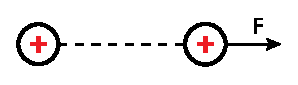
\includegraphics[width=2in]{modules/m0002_fTwoChargedParticles.eps}
}}{Two circles with red plus signs in the middle to indicate their positive charge. They are some distance apart on the same horizontal axis indicated by a dashed line. An arrow labeled "F" is emanating from the rightmost particle and points to the right.}
\end{center}  
\centerline{\scriptsize 
\copyright~\hyperref[m0002_fTwoChargedParticles_Credit]{M.\ Goldammer} 
\href{https://creativecommons.org/licenses/by-sa/4.0/}{CC BY~SA 4.0} 
} 
\caption{
\label{m0002_fTwoChargedParticles}
A positively-charged particle experiences a repulsive force ${\bf F}$ in the presence of another particle which is also positively-charged.
% https://commons.wikimedia.org/wiki/File:M0002_fTwoChargedParticles.svg
}
\end{figure}

Now let us revisit the original one particle scenario.  In that scenario, we could make a map in which every position in space is assigned a vector that describes the force that a particle having a specified charge $q$ would experience if it were to appear there.  
The result looks something like Figure~\ref{m0002_fForceMap}. 
This map of force vectors is essentially a description of the electric field associated with the first particle.
%
\begin{figure}
\begin{center}
\pdftooltip{{  % note double braces
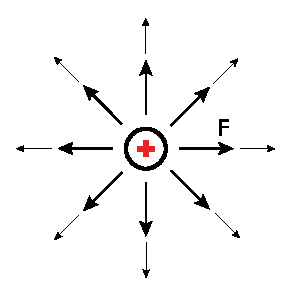
\includegraphics[width=2in]{modules/m0002_fForceMap.eps}
}}{A single circle with a red plus sign in it represents a positive charge. There are 8 arrows with a magnitude of "F" equidistantly spaced, emanating outward from the perimeter of the circle. Each of these arrows has a smaller arrow emanating from it.}
\end{center} 
\centerline{\scriptsize 
\copyright~\hyperref[m0002_fForceMap_Credit]{M.\ Goldammer} 
\href{https://creativecommons.org/licenses/by-sa/4.0/}{CC BY~SA 4.0} 
} 
\caption{
\label{m0002_fForceMap}
A map of the force that would be experienced by a second particle having a positive charge.  Here, the magnitude and direction of the force is indicated by the size and direction of the arrow.
% https://commons.wikimedia.org/wiki/File:M0002_fForceMap.svg
}
\end{figure}
 
There are many ways in which the electric field may be quantified. 
Electric field intensity ${\bf E}$ is simply one of these ways.  
We define ${\bf E}({\bf r})$ to be the force 
\index{force}
${\bf F}({\bf r})$ experienced by a test particle having charge $q$, divided by $q$; i.e.,  
%
\begin{equation}
{\bf E}({\bf r}) \triangleq \lim_{q \to 0} \frac{{\bf F}({\bf r})}{q}
\label{m0002_eEDef1}
\end{equation} 
%
Note that it is required for the charge to become vanishingly small (as indicated by taking the limit) in order for this definition to work.  
This is because the source of the electric field is charge, so the test particle contributes to the total electric field.  
To accurately measure the field of interest, the test charge must be small enough not to significantly perturb the field. 
This makes Equation~\ref{m0002_eEDef1} awkward from an engineering perspective, and we'll address that later in this section. 

According the definition of Equation~\ref{m0002_eEDef1}, the units of ${\bf E}$ are those of force divided by charge.  The SI units for force and charge are the newton (N) and coulomb (C) respectively, so ${\bf E}$ has units of N/C.  However, we typically express ${\bf E}$ in units of V/m, not N/C.  What's going on?  The short answer is that 1~V/m $=$ 1~N/C:
$$ 
\frac{\mbox{N}}{\mbox{C}} =
\frac{\mbox{N}\cdot\mbox{m}}{\mbox{C}\cdot\mbox{m}} =
\frac{\mbox{J}}{\mbox{C}\cdot\mbox{m}} =
\frac{\mbox{V}}{\mbox{m}}
$$
where we have used the fact that 1~N$\cdot$m $=$ 1~joule (J) of energy and 1~J/C $=$ 1~V. 

%ORB HIGHLIGHT
\begin{mdframed}[backgroundcolor=yellow!20,nobreak=true] 
Electric field intensity (${\bf E}$, N/C or V/m) 
\index{electric field intensity!definition}
is a vector field that quantifies the force experienced by a charged particle due to the influence of charge not associated with that particle. 
\end{mdframed}

The analysis of units doesn't do much to answer the question of why we should prefer to express ${\bf E}$ in V/m as opposed to N/C.
Let us now tackle that question.

Figure~\ref{m0002_fBatCap} shows a simple thought experiment that demonstrates the concept of electric field intensity in terms of an electric circuit.  
This circuit consists of a parallel-plate capacitor 
\index{capacitor!parallel plate}
in series with a 9~V battery.\footnote{It is not necessary to know anything about capacitors to get to the point, so no worries!}
The effect of the battery, connected as shown, is to force an accumulation of positive charge on the upper plate, and an accumulation of negative charge on the lower plate.  If we consider the path from the position labeled ``A,'' along the wire and through the battery to the position labeled ``B,'' the change in electric potential is $+9$~V.  It must also be true that the change in electric potential as we travel from B to A through the capacitor is $-9$~V, since the sum of voltages over any closed loop in a circuit is zero.  Said differently, the change in electric potential between the plates of the capacitor, starting from node A and ending at node B, is $+9$~V.  Now, note that the spacing between the plates in the capacitor is 1~mm.   
Thus, the rate of change of the potential between the plates is 9~V divided by 1~mm, which is 9000~V/m. 
This is literally the electric field intensity between the plates. 
That is, if one places a particle with an infinitesimally-small charge between the plates (point ``C''), and then measures the ratio of force to charge, one finds it is 9000~N/C pointing toward A.  We come to the following remarkable conclusion:
%
\begin{figure}
\begin{center}
\pdftooltip{{  % note double braces
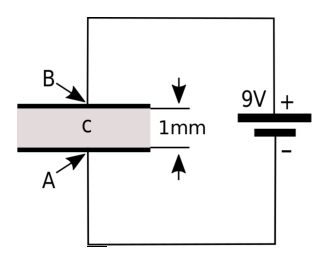
\includegraphics[width=2in]{modules/m0002_fBatCap.eps} 
% https://commons.wikimedia.org/wiki/File:M0002_fBatCap.svg
}}{Parallel plates joined in series with 9V battery. Upper plate labeled B, lower plate labeled A, and point between plates labeled C. Plates are 1 mm apart.}
\end{center}
\centerline{\scriptsize 
\copyright~\hyperref[m0002_fBatCap_Credit]{Y.\ Qin} 
\href{https://creativecommons.org/licenses/by/3.0/}{CC BY 3.0} 
} 
\caption{
\label{m0002_fBatCap}
A simple circuit used to describe the concept of electric field intensity. In this example, ${\bf E}$ at point C is 9000~V/m directed from B toward A. 
}
\end{figure}

%ORB HIGHLIGHT
\begin{mdframed}[backgroundcolor=yellow!20,nobreak=true] 
${\bf E}$ points in the direction in which electric potential is most rapidly decreasing, and the magnitude of ${\bf E}$ is the rate of change in electric potential with distance in this direction.  
\end{mdframed}

The reader may have noticed that we have defined the electric field in terms of what it \emph{does}.
We have have not directly addressed the question of what the electric field \emph{is}.  
This is the best we can do using classical physics, and
fortunately, this is completely adequate for the most engineering applications.
However, a deeper understanding is possible using quantum mechanics, 
\index{quantum mechanics}
where we find that the electric field and the magnetic field are in fact manifestations of the same fundamental force, aptly named the \emph{electromagnetic force}.
\index{electromagnetic force}
(In fact, the electromagnetic force is found to be one of just four fundamental forces, the others being \emph{gravity}, the \emph{strong nuclear force}, and the \emph{weak nuclear force}.)
Quantum mechanics also facilitates greater insight into the nature of electric charge and of the \emph{photon}, 
\index{photon}
which is the fundamental constituent of electromagnetic waves.  
For more information on this topic, an excellent starting point is the video ``Quantum Invariance \& The Origin of The Standard Model'' referenced at the end of this section.

%%%%%%%%%%%%%%%%%%%%%%%%%%

{\bf Additional Reading:}
\begin{itemize}
\item ``\href{https://en.wikipedia.org/wiki/Electric_field}{Electric field}'' on Wikipedia.
\item PBS Space Time video ``\href{https://youtu.be/V5kgruUjVBs}{Quantum Invariance} \& The Origin of The Standard Model,'' on YouTube.
\end{itemize}

\index{electric field intensity|)}
\index{field!electric|)}

      \vfill\break
    \section{Permittivity}
{\color{blue}\tiny[m0008]}      % This is text associated with the open textbook "Open Electromagnetics"
% See immediately below for author, date
% <License info goes here (boilerplate, not read by project compiler)>

%ORB TITLE Permittivity    
%ORB AUTHOR 0       # S.W. Ellingson, Virginia Tech (ellingson@vt.edu)
%ORB DATE   20180731
%ORB ABSTRACT Introduction to permittivity, using concept of relationship between electric field intensity and charge

\label{m0008_Permittivity} % <-- Must match name of this file and module directory name.  Don't mess with this!
\index{permittivity|(}

Permittivity describes the effect of material in determining the electric field in response to electric charge.  For example, one can observe from laboratory experiments %\footnote{Also worth noting that this equation also follows directly from Maxwell's Equations, described in the next chapter.} 
that a particle having charge $q$ gives rise to the electric field 
%
\begin{equation}
{\bf E} = \hat{\bf R} ~ q ~ \frac{1}{4\pi R^2} ~ \frac{1}{\epsilon}
\end{equation}
%
where $R$ is distance from the charge, 
$\hat{\bf R}$ is a unit vector pointing away from the charge,
and $\epsilon$ is a constant that depends on the material.
Note that ${\bf E}$ increases with $q$, which makes sense since electric charge is the source of ${\bf E}$.  
Also note that ${\bf E}$ is inversely proportional to $4\pi R^2$, indicating that ${\bf E}$ decreases in proportion to the area of a sphere surrounding the charge -- a principle commonly known as the \emph{inverse square law}.
\index{inverse square law}
The remaining factor $1/\epsilon$ is the constant of proportionality, which captures the effect of material.   
Given units of V/m for ${\bf E}$ and C for $Q$, we find that $\epsilon$ must have units of farads per meter (F/m). 
(To see this, note that 1~F $=$ 1~C/V.)    

%ORB HIGHLIGHT
\begin{mdframed}[backgroundcolor=yellow!20,nobreak=true] 
Permittivity ($\epsilon$, F/m) describes the effect of material in determining the electric field intensity in response to charge. 
\end{mdframed}

In free space (that is, a perfect vacuum), we find that $\epsilon = \epsilon_0$ where:
%
\begin{equation}
\epsilon_0 \cong 8.854 \times 10^{-12} ~\mbox{F/m}
\end{equation}
% 
The permittivity of air is only slightly greater, and usually can be assumed to be equal to that of free space.
In most other materials, the permittivity is significantly greater; that is, the same charge results in a weaker electric field intensity.  

It is common practice to describe the permittivity of materials relative to the permittivity of free space.
This \emph{relative permittivity} 
\index{permittivity!relative}
\index{relative permittivity|see{permittivity, relative}}
is given by:
%
\begin{equation}
\epsilon_r \triangleq \frac{\epsilon}{\epsilon_0}
\end{equation}
%  
Values of $\epsilon_r$ for a few representative materials is given in Appendix~\ref{m0135_Table_of_Permittivities}.  
Note that $\epsilon_r$ ranges from 1 (corresponding to a perfect vacuum) to about 60 or so in common engineering applications.  
Also note that relative permittivity is sometimes referred to as \emph{dielectric constant}. 
\index{dielectric constant}
This term is a bit misleading, however, since permittivity is a meaningful concept for many materials that are not dielectrics.

%%%%%%%%%%%%%%%%%

{\bf Additional Reading:}
\begin{itemize}
\item ``\href{https://en.wikipedia.org/wiki/Permittivity}{Permittivity}'' on Wikipedia.
\item Appendix~\ref{m0135_Table_of_Permittivities} (``Permittivity of Some Common Materials'').
\item ``\href{https://en.wikipedia.org/wiki/Inverse-square_law}{Inverse square law}'' on Wikipedia.
\end{itemize}

\index{permittivity|)}



      \vfill\break
    \section{Electric Flux Density}
{\color{blue}\tiny[m0011]}      % This is text associated with the open textbook "Open Electromagnetics"
% See immediately below for author, date
% <License info goes here (boilerplate, not read by project compiler)>

%ORB TITLE Electric Flux Density  
%ORB AUTHOR 0       # S.W. Ellingson, Virginia Tech (ellingson@vt.edu)
%ORB DATE   20180731 
%ORB ABSTRACT Introduction to electric flux density

\label{m0011_Electric_Flux_Density} % <-- Must match name of this file and module directory name.  Don't mess with this!
\index{electric flux density|(}
\index{field!electric|(}
\index{flux density, electric|see{electric flux density}}

Electric flux density, assigned the symbol ${\bf D}$, is an alternative to electric field intensity (${\bf E}$) as a way to quantify an electric field.
This alternative description offers some actionable insight, as we shall point out at the end of this section.

First, what is electric flux density?
Recall that a particle having charge $q$ gives rise to the electric field intensity
%
\begin{equation}
{\bf E} = \hat{\bf R} ~ q ~ \frac{1}{4\pi R^2} ~ \frac{1}{\epsilon}
\label{m0011_eEparticle1}
\end{equation}
%
where $R$ is distance from the charge and $\hat{\bf R}$ points away from the charge.
Note that ${\bf E}$ is inversely proportional to $4\pi R^2$, indicating that ${\bf E}$ decreases in proportion to the area of a sphere surrounding the charge.
Now integrate both sides of Equation~\ref{m0011_eEparticle1} over a sphere $\mathcal{S}$ of radius $R$:
%
\begin{equation}
\oint_{\mathcal{S}} {\bf E}({\bf r}) \cdot d{\bf s} = \oint_{\mathcal{S}} \left[ \hat{\bf R} ~ q ~ \frac{1}{4\pi R^2} ~ \frac{1}{\epsilon} \right] \cdot d{\bf s}
\end{equation}
%
Factoring out constants that do not vary with the variables of integration, the right-hand side becomes:
%
\begin{equation}
q ~ \frac{1}{4\pi R^2} ~ \frac{1}{\epsilon} ~ \oint_{\mathcal{S}} \hat{\bf R} \cdot d{\bf s}
\nonumber
\end{equation}
%
Note that $d{\bf s}=\hat{\bf R}ds$ in this case, and also that $\hat{\bf R}\cdot\hat{\bf R}=1$.  Thus, the right-hand side simplifies to:
%
\begin{equation}
q ~ \frac{1}{4\pi R^2} ~ \frac{1}{\epsilon} ~ \oint_{\mathcal{S}} ~ds
\nonumber
\end{equation}
%
The remaining integral is simply the area of $\mathcal{S}$, which is $4\pi R^2$.  Thus, we find:
%
\begin{equation}
\oint_{\mathcal{S}} {\bf E}({\bf r}) \cdot d{\bf s} = \frac{q}{\epsilon}
\label{m0011_eEparticle2}
\end{equation}
%
The integral of a vector field over a specified surface is known as \emph{flux} 
\index{flux}
(see ``Additional Reading'' at the end of this section). 
Thus, we have found that the flux of ${\bf E}$ through the sphere $\mathcal{S}$ is equal to a constant, namely $q/\epsilon$.
Furthermore, this constant is the same regardless of the radius $R$ of the sphere.
Said differently, the flux of ${\bf E}$ is constant with distance, and does not vary as ${\bf E}$ itself does.  
Let us capitalize on this observation by making the following small modification to Equation~\ref{m0011_eEparticle2}:
%
\begin{equation}
\oint_{\mathcal{S}} \left[\epsilon {\bf E}\right] \cdot d{\bf s} = q
\end{equation}
%
In other words, the flux of the quantity $\epsilon {\bf E}$ is equal to the enclosed charge, regardless of the radius of the sphere over which we are doing the calculation.
This leads to the following definition:

%ORB HIGHLIGHT
\begin{mdframed}[backgroundcolor=yellow!20,nobreak=true] 
The electric flux density 
\index{electric flux density!definition}
${\bf D} = \epsilon {\bf E}$, having units of C/m$^2$, is a description of the electric field in terms of flux, as opposed to force or change in electric potential. 
\end{mdframed}

It may appear that ${\bf D}$ is redundant information given ${\bf E}$ and $\epsilon$, but this is true only in homogeneous media.
\index{homogeneous (media)}
The concept of electric flux density becomes important -- and decidedly not redundant -- when we encounter boundaries between media having different permittivities.  
As we shall see in Section~\ref{m0021_Boundary_Conditions_on_D}, boundary conditions on ${\bf D}$ constrain the component of the electric field that is perpendicular to the boundary separating two regions.  If one ignores the ``flux'' character of the electric field represented by ${\bf D}$ and instead considers only ${\bf E}$, then only the \emph{tangential} component of the electric field is constrained.  
In fact, when one of the two materials comprising the boundary between two material regions is a perfect conductor, 
\index{conductor!perfect}
\index{perfect conductor|see{conductor, perfect}}
then the electric field is \emph{completely determined} by the boundary condition on ${\bf D}$.  This greatly simplifies the problem of finding the electric field in a region bounded or partially bounded by materials that can be modeled as perfect conductors, including many metals.  In particular, this principle makes it easy to analyze capacitors. 
 
We conclude this section with a warning.
Even though the SI units for ${\bf D}$ are C/m$^2$, ${\bf D}$ describes an electric field and \emph{not} a surface charge density.
It is certainly true that one may describe the amount of charge distributed over a surface using units of C/m$^2$.
However, ${\bf D}$ is not necessarily a description of \emph{actual} charge, and there is no implication that the source of the electric field is a distribution of surface charge.
On the other hand, it \emph{is} true that ${\bf D}$ can be interpreted as an \emph{equivalent} surface charge density that would give rise to the observed electric field, and in some cases, this equivalent charge density turns out to be the actual charge density. 

%%%%%%%%%%%%%%%%%%%%%%%%%%

{\bf Additional Reading:}
\begin{itemize}
\item ``\href{https://en.wikipedia.org/wiki/Flux}{Flux}'' on Wikipedia.
\end{itemize}

\index{electric flux density|)}
\index{field!electric|)}

      \vfill\break
    \section{Magnetic Flux Density}
{\color{blue}\tiny[m0003]}      % This is text associated with the open textbook "Open Electromagnetics"
% See immediately below for author, date
% <License info goes here (boilerplate, not read by project compiler)>

%ORB TITLE Magnetic Flux Density
%ORB AUTHOR 0        # S.W. Ellingson, Virginia Tech (ellingson@vt.edu)
%ORB DATE 20180731   # yyyymmdd
%ORB ABSTRACT 

\label{m0003_Magnetic_Flux_Density} % <-- Must match name of this file and module directory name.  Don't mess with this!
\index{magnetic flux density|(}
\index{field!magnetic|(}
\index{flux density, magnetic|see{magnetic flux density}}

\emph{Magnetic flux density} is a vector field which we identify using the symbol ${\bf B}$ and which has SI units of tesla (T).  
Before offering a formal definition, it is useful to consider the broader concept of the \emph{magnetic field}.

Magnetic fields are an intrinsic property of some materials, most notably permanent magnets.
\index{permanent magnet}  
The basic phenomenon is probably familiar, and is shown in Figure~\ref{m0003_fBarMagnet}.
A bar magnet has ``poles'' identified as ``N'' (``north'') and ``S'' (``south'').
The N-end of one magnet attracts the S-end of another magnet but repels the N-end of the other magnet and so on.
The existence of a vector field is apparent since the observed force acts at a distance and is asserted in a specific direction.  
In the case of a permanent magnet, the magnetic field arises from mechanisms occurring at the scale of the atoms and electrons comprising the material.  
These mechanisms require some additional explanation which we shall defer for now.  
%
\begin{figure}[b!]
\begin{center}
\pdftooltip{{  % note double braces
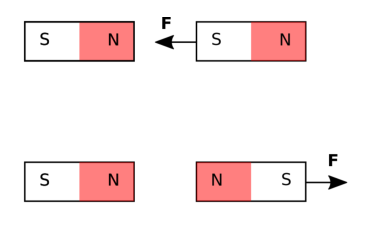
\includegraphics[width=2in]{modules/m0003_fBarMagnet.eps} 
% https://commons.wikimedia.org/wiki/File:M0003_fBarMagnet.svg
}}{Two pairs of bar magnets shown horizontally, one pair above the other: The top pair is oriented so that the "north" end of the left magnet is closest to the "south" end of the right magnet. An arrow labeled "F" points left from the "south" end of the right magnet toward the north end of the left magnet. The bottom pair is oriented so the "north" ends of both magnets are pointed toward each other. An arrow labeled "F" points right from the south end of the right magnet.}
\end{center}
\centerline{\scriptsize 
\copyright~\hyperref[m0003_fBarMagnet_Credit]{Y.\ Qin} 
\href{https://creativecommons.org/licenses/by/3.0/}{CC BY 3.0} 
} 
\caption{
\label{m0003_fBarMagnet}
Evidence of a vector field from observations of the force perceived by the bar magnets on the right in the presence of the bar magnets on the left.
}
\end{figure}

Magnetic fields also appear in the presence of current.
\index{current}
For example, a coil of wire bearing a current is found to influence permanent magnets (and vice versa) in the same way that permanent magnets affect each other.
This is shown in Figure~\ref{m0003_fCoilBarMagnet}.
From this, we infer that the underlying mechanism is the same -- i.e., the vector field generated by a current-bearing coil is the same phenomenon as the vector field associated with a permanent magnet.
Whatever the source, %we name this field ${\bf B}$ and
we are now interested in quantifying its behavior. 
%
\begin{figure}
\begin{center}
\pdftooltip{{  % note double braces
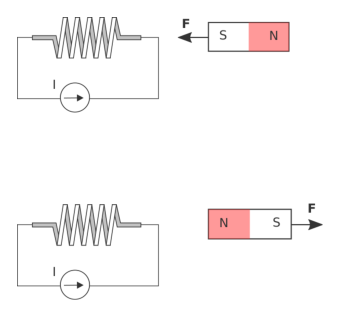
\includegraphics[width=2.5in]{modules/m0003_fCoilBarMagnet.eps}
% https://commons.wikimedia.org/wiki/File:M0003_fCoilBarMagnet.svg
}}{Two identical circuits, one above the other: A current source is connected in series with a coil of wire. Current is flowing in the counterclockwise direction. To the right of the top coil is a horizontal bar magnet with the south pole closest to the coil. An arrow labeled "F" points from the south pole towards the coil. To the right of the bottom coil is another horizontal bar magnet with the north pole closest to the coil. An arrow labeled "F" points away from the coil from the south pole.}
\end{center} 
\centerline{\scriptsize 
\copyright~\hyperref[m0003_fCoilBarMagnet_Credit]{Y.\ Qin} 
\href{https://creativecommons.org/licenses/by/4.0/}{CC BY 4.0} 
} 
\caption{
\label{m0003_fCoilBarMagnet}
Evidence that current can also create a magnetic field.
}
\end{figure}

To begin, let us consider the effect of a magnetic field on a electrically-charged particle.
First, imagine a region of free space with no electric or magnetic fields.
Next, imagine that a charged particle appears.  
This particle will experience no force.
Next, a magnetic field appears; perhaps this is due to a permanent magnet or a current in the vicinity.
This situation is shown in Figure~\ref{m0003_fFqvB} (top).
Still, no force is applied to the particle.
In fact, nothing happens until the particle in set in motion.
Figure~\ref{m0003_fFqvB} (bottom) shows an example. Suddenly, the particle perceives a force. 
We'll get to the details about direction and magnitude in a moment, but
the main idea is now evident. A magnetic field is something that applies a force to a charged particle in motion, distinct from (in fact, in addition to) the force associated with an electric field.  
%
\begin{figure}
\begin{center}
\pdftooltip{{  % note double braces
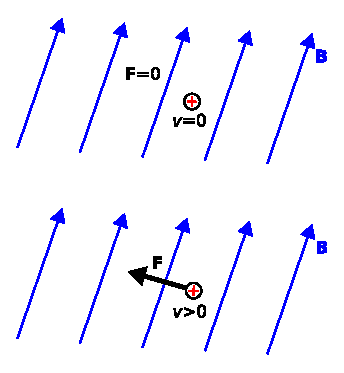
\includegraphics[width=2in]{modules/m0003_fFqvB.eps}
% https://commons.wikimedia.org/wiki/File:M0003_fFqvB.svg
}}{Two identical magnetic fields, one above the other. Magnetic field, B,  is represented by five parallel arrows of equal magnitude, pointing to the right at an arbitrary angle. In both fields, a circle with a red plus sign sits between the third and fourth arrows. In the top diagram, the circle with a red plus is labeled with "F = 0" and "v = 0". In the bottom diagram the circle with the red plus has an arrow labeled "F" emanating from it that is perpendicular to the magnetic field arrows. It is labeled "v > 0".}
\end{center} 
\centerline{\scriptsize 
\copyright~\hyperref[m0003_fFqvB_Credit]{Y.\ Qin} 
\href{https://creativecommons.org/licenses/by/4.0/}{CC BY 4.0} 
} 
\caption{
\label{m0003_fFqvB}
The force perceived by a charged particle that is (\emph{top}) motionless and (\emph{bottom}) moving with velocity ${\bf v}=\hat{\bf z}v$, which is perpendicular to the plane of this document and toward the reader.
}
\end{figure}

Now, it is worth noting that a single charged particle in motion is the simplest form of current. 
Remember also that motion is required for the magnetic field to influence the particle. 
Therefore, not only is current the source of the magnetic field, the magnetic field also exerts a force on current.  
Summarizing:

%ORB HIGHLIGHT
\begin{mdframed}[backgroundcolor=yellow!20,nobreak=true] 
The magnetic field describes the force exerted on permanent magnets and currents in the presence of other permanent magnets and currents.     
\end{mdframed}

So, how can we quantify a magnetic field?
The answer from classical physics involves another experimentally-derived equation that predicts force as a function of charge, velocity, and a vector field ${\bf B}$ representing the magnetic field.
Here it is:
The force 
\index{force}
applied to a particle bearing charge $q$ is 
%
\begin{equation}
%{\bf F}({\bf r}) = q{\bf v} \times {\bf B}({\bf r})
{\bf F} = q{\bf v} \times {\bf B}
\label{m0005_eFqvB}
\end{equation}  
%
where ${\bf v}$ is the velocity of the particle and 
``$\times$'' denotes the cross product.  
The cross product of two vectors is in a direction perpendicular to each of the two vectors, so the force exerted by the magnetic field is perpendicular to both the direction of motion and the direction in which the magnetic field points.

The reader would be well-justified in wondering why the force exerted by the magnetic field should \emph{perpendicular} to ${\bf B}$.  
For that matter, why should the force depend on {\bf v}?
These are questions for which classical physics provides no obvious answers. 
Effective answers to these questions require concepts from quantum mechanics,
\index{quantum mechanics}
where we find that the magnetic field is a manifestation of the fundamental and aptly-named \emph{electromagnetic force}.
\index{electromagnetic force}
The electromagnetic force also gives rises to the electric field, and it is only limited intuition, grounded in classical physics, that leads us to perceive the electric and magnetic fields as distinct phenomena. 
For our present purposes -- and for most commonly-encountered engineering applications -- we do not require these concepts.
It is sufficient to accept this apparent strangeness as fact and proceed accordingly.
%These are simply two of the ways in which the magnetic field is strange.
%\footnote{To appreciate how truly strange this is, imagine the following analogy:  When standing still in the middle of a field you feel no force.  Then you begin to walk.  Suddenly the wind begins to blow.  The faster you walk, the harder the wind blows. How does the wind know?}

Dimensional analysis of Equation~\ref{m0005_eFqvB} reveals that ${\bf B}$ has units of (N$\cdot$s)/(C$\cdot$m).  
In SI, this combination of units is known as the tesla (T). 

We refer to ${\bf B}$ as \emph{magnetic flux density}, and therefore tesla is a unit of magnetic flux density.
A fair question to ask at this point is: What makes this a flux density?
The short answer is that this terminology is somewhat arbitrary, and in fact is not even uniformly accepted.
In engineering electromagnetics, the preference for referring to ${\bf B}$ as a ``flux density'' is because we frequently find ourselves integrating ${\bf B}$ over a mathematical surface.  
Any quantity that is obtained by integration over a surface is referred to as ``flux,''
\index{flux}
and so it becomes natural to think of ${\bf B}$ as a flux density; i.e., as flux per unit area.  
The SI unit for magnetic flux is the weber (Wb).
Therefore, ${\bf B}$ may alternatively be described as having units of Wb/m$^2$, and 1~Wb/m$^2$ $=$ 1~T.

%ORB HIGHLIGHT
\begin{mdframed}[backgroundcolor=yellow!20,nobreak=true] 
Magnetic flux density 
\index{magnetic flux density!definition}
(${\bf B}$, T or Wb/m$^2$) is a description of the magnetic field that can be defined as the solution to Equation~\ref{m0005_eFqvB}. 
\end{mdframed}

When describing magnetic fields, we occasionally refer to the concept of a \emph{field line}, defined as follows:

%ORB HIGHLIGHT
\begin{mdframed}[backgroundcolor=yellow!20,nobreak=true] 
A magnetic field line 
\index{field line (magnetic)}
is the curve in space traced out by following the direction in which the magnetic field vector points. 
\end{mdframed}

This concept is illustrated in 
Figure~\ref{m0003_fFieldLinesBarMagnet} for a permanent bar magnet and 
Figure~\ref{m0003_fFieldLinesCoil} for a current-bearing coil. 
%
\begin{figure}
\begin{center}
\pdftooltip{{  % note double braces
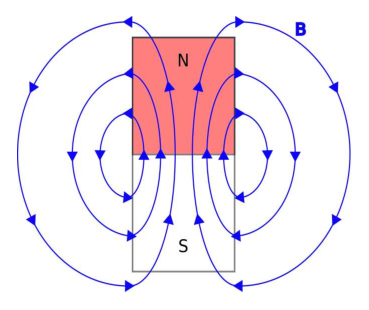
\includegraphics[width=2.5in]{modules/m0003_fFieldLinesBarMagnet.eps}
% https://commons.wikimedia.org/wiki/File:M0003_fFieldLinesBarMagnet.svg
}}{A bar magnet oriented vertically with the north pole at the top. The magnetic field is shown by two sets of concentric curves labeled "B" that mirror each other on the left and right sides of the magnet. They are centered on the horizontal axis where the north and south poles meet. The left-side curves have arrows pointing counterclockwise. The right-side curves have clockwise pointing arrows.}
\end{center} 
\centerline{\scriptsize 
\copyright~\hyperref[m0003_fFieldLinesBarMagnet_Credit]{Y.\ Qin} 
\href{https://creativecommons.org/licenses/by/4.0/}{CC BY 4.0} 
} 
\caption{
\label{m0003_fFieldLinesBarMagnet}
The magnetic field of a bar magnet, illustrating field lines.
}
\end{figure}
%
\begin{figure}
\begin{center}
\pdftooltip{{  % note double braces
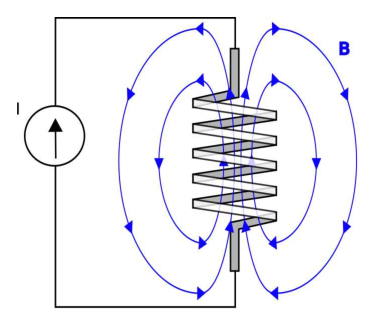
\includegraphics[width=2.5in]{modules/m0003_fFieldLinesCoil.eps}
% https://commons.wikimedia.org/wiki/File:0003_fFieldLinesCoil.svg
}}{A series circuit with a current source and a wire coil which is oriented vertically. Current is flowing clockwise. The field lines are similar to those in an earlier figure, but this time centered on the middle of the coil.}
\end{center} 
\centerline{\scriptsize 
\copyright~\hyperref[m0003_fFieldLinesCoil_Credit]{Y.\ Qin} 
\href{https://creativecommons.org/licenses/by/4.0/}{CC BY 4.0} 
} 
\caption{
\label{m0003_fFieldLinesCoil}
The magnetic field of a current-bearing coil, illustrating field lines.
}
\end{figure}

Magnetic field lines are remarkable for the following reason:
%
%ORB HIGHLIGHT
\begin{mdframed}[backgroundcolor=yellow!20,nobreak=true] 
A magnetic field line always forms a closed loop. 
\end{mdframed}
%
This is true in a sense even for field lines which seem to form straight lines (for example, those along the axis of the bar magnet and the coil in Figures~\ref{m0003_fFieldLinesBarMagnet} and \ref{m0003_fFieldLinesCoil}), since a field line that travels to infinity in one direction reemerges from infinity in the opposite direction.

%%%%%%%%%%%%%%%%%%%%%%%%%%%

{\bf Additional Reading:}
\begin{itemize}
\item ``\href{https://en.wikipedia.org/wiki/Magnetic_field}{Magnetic Field}'' on Wikipedia.
\end{itemize}

\index{magnetic flux density|)}
\index{field!magnetic|)}

      \vfill\break
    \section{Permeability}
{\color{blue}\tiny[m0009]}      % This is text associated with the open textbook "Open Electromagnetics"
% See immediately below for author, date
% <License info goes here (boilerplate, not read by project compiler)>

%ORB TITLE Permeability
%ORB AUTHOR 0        # S.W. Ellingson, Virginia Tech (ellingson@vt.edu)
%ORB DATE 20180731   # yyyymmdd
%ORB ABSTRACT 

\label{m0009_Permeability} % <-- Must match name of this file and module directory name.  Don't mess with this!
\index{permeability|(}

Permeability describes the effect of material in determining the magnetic flux density.  
All else being equal, magnetic flux density increases in proportion to permeability.
 
To illustrate the concept, consider that a particle bearing charge $q$ moving at velocity ${\bf v}$ gives rise to a magnetic flux density:
%
\begin{equation}
{\bf B}({\bf r}) = \mu ~ \frac{q {\bf v}}{4\pi R^2} \times \hat{\bf R}
%\label{eMatB}
\end{equation}
%
where $\hat{\bf R}$ is the unit vector pointing from the charged particle to the field point ${\bf r}$, $R$ is this distance, and ``$\times$'' is the cross product.
Note that ${\bf B}$ increases with charge and speed, which makes sense since moving charge is the source of the magnetic field.  
Also note that ${\bf B}$ is inversely proportional to $4\pi R^2$, indicating that $\left|{\bf B}\right|$ decreases in proportion to the area of a sphere surrounding the charge, also known as the {\it inverse square law}.
\index{inverse square law}
The remaining factor, $\mu$, is the constant of proportionality that captures the effect of material.
We refer to $\mu$ as the \emph{permeability} of the material.
Since ${\bf B}$ can be expressed in units of Wb/m$^2$ and the units of ${\bf v}$ are m/s, we see that $\mu$ must have units of henries per meter (H/m). 
(To see this, note that 1~H $\triangleq$ 1~Wb/A.)   

%ORB HIGHLIGHT
\begin{mdframed}[backgroundcolor=yellow!20,nobreak=true] 
Permeability ($\mu$, H/m) describes the effect of material in determining the magnetic flux density. 
\end{mdframed}

In free space, we find that the permeability $\mu=\mu_0$ where:
%
\begin{equation}
\mu_0 = 4\pi \times 10^{-7} ~\mbox{H/m}
\end{equation}
% 
It is common practice to describe the permeability of materials in terms of their {\it relative permeability}:
\index{permeability!relative}
\index{relative permeability|see{permeability, relative}}
%
\begin{equation}
\mu_r \triangleq \frac{\mu}{\mu_0}
\end{equation}
%
which gives the permeability relative to the minimum possible value; i.e., that of free space.  Relative permeability for a few representative materials is given in Appendix~\ref{m0136_Table_of_Permeabilities}.  

Note that $\mu_r$ is approximately 1 for all but a small class of materials.  These are known as {\it magnetic materials}, and may exhibit values of $\mu_r$ as large as $\sim 10^6$.  
A commonly-encountered category of magnetic materials is \emph{ferromagnetic} material, of which the best-known example is iron.  

%%%%%%%%%%%%%%%%%%%%%

{\bf Additional Reading:}
\begin{itemize}
\item ``\href{https://en.wikipedia.org/wiki/Permeability_(electromagnetism)}{Permeability (electromagnetism)}'' on Wikipedia.
\item Section~\ref{m0058_Magnetic_Materials} (``Magnetic Materials'').
\item Appendix~\ref{m0136_Table_of_Permeabilities} (``Permeability of Some Common Materials'').
\end{itemize}

\index{permeability|)}

      \vfill\break
    \section{Magnetic Field Intensity}
{\color{blue}\tiny[m0012]}      % This is text associated with the open textbook "Open Electromagnetics"
% See immediately below for author, date
% <License info goes here (boilerplate, not read by project compiler)>

%ORB TITLE Magnetic Field Intensity 
%ORB AUTHOR 0        # S.W. Ellingson, Virginia Tech (ellingson@vt.edu)
%ORB DATE 20180731   # yyyymmdd
%ORB ABSTRACT 
 
\label{m0012_Magnetic_Field_Intensity} % <-- Must match name of this file and module directory name.  Don't mess with this!
\index{magnetic field intensity|(}
\index{field!magnetic|(}
\index{field intensity, magnetic|see{magnetic field intensity}}

Magnetic field intensity ${\bf H}$ is an alternative description of the magnetic field in which the effect of material is factored out.  
For example, the magnetic flux density ${\bf B}$ (reminder: Section~\ref{m0003_Magnetic_Flux_Density}) due to a point charge $q$ moving at velocity ${\bf v}$ can be written in terms of the \emph{Biot-Savart Law}:
\index{Biot-Savart Law}
%
\begin{equation}
{\bf B} = \mu ~ \frac{q {\bf v}}{4\pi R^2} \times \hat{\bf R}
\label{m0012_eMatB}
\end{equation}
%
where $\hat{\bf R}$ is the unit vector pointing from the charged particle to the field point ${\bf r}$, $R$ is this distance, ``$\times$'' is the cross product, and
$\mu$ is the permeability of the material.
We can rewrite Equation~\ref{m0012_eMatB} as: 
%
\begin{equation}
{\bf B} \triangleq \mu {\bf H}
\label{m0012_eHDef}
\end{equation}
%
with:
%
\begin{equation}
{\bf H} =  \frac{q {\bf v}}{4\pi R^2} \times \hat{\bf R}
\label{m0012_eHHH}
\end{equation}
%
so ${\bf H}$ in homogeneous media 
\index{homogeneous (media)}
does not depend on $\mu$.

Dimensional analysis of Equation~\ref{m0012_eHHH} reveals that the units for ${\bf H}$ are amperes per meter (A/m).  
However, ${\bf H}$ does not represent surface current density,\footnote{The concept of current density is not essential to understand this section; however, a primer can be found in Section~\ref{m0101_Current_Distributions}.} as the units might suggest.  
While it is certainly true that a distribution of current (A) over some linear cross-section (m) can be described as a current density having units of A/m, ${\bf H}$ is associated with the magnetic field and not a particular current distribution.
Said differently, ${\bf H}$ can be viewed as a description of the magnetic field in terms of an equivalent (but not actual) current.

%ORB HIGHLIGHT
\begin{mdframed}[backgroundcolor=yellow!20,nobreak=true] 
The magnetic field intensity 
\index{magnetic field intensity!definition}
${\bf H}$ (A/m), defined using Equation~\ref{m0012_eHDef}, is a description of the magnetic field independent from material properties. 
\end{mdframed}

It may appear that ${\bf H}$ is redundant information given ${\bf B}$ and $\mu$, but this is true only in homogeneous
media. The concept of magnetic field intensity becomes important -- and decidedly not redundant -- when we encounter boundaries between media having different permeabilities.
As we shall see in Section~\ref{m0023_Boundary_Conditions_on_H}, boundary conditions on ${\bf H}$ constrain the component of the magnetic field which is tangent to the boundary separating two otherwise-homogeneous regions.
If one ignores the characteristics of the magnetic field represented by ${\bf H}$ and instead
considers only ${\bf B}$, then only the perpendicular component of the magnetic field is constrained.

The concept of magnetic field intensity also turns out to be useful in a certain problems in which $\mu$ is not a constant, but rather is a function of magnetic field strength.  In this case, the magnetic behavior of the material is said to be \emph{nonlinear}. 
\index{nonlinear (media)}
For more on this, see Section~\ref{m0058_Magnetic_Materials}. 
 
%%%%%%%%%%%%%%%%%%%

{\bf Additional Reading:}
\begin{itemize}
\item ``\href{https://en.wikipedia.org/wiki/Magnetic_field}{Magnetic field}'' on Wikipedia.
\item ``\href{https://en.wikipedia.org/wiki/Biot-Savart_law}{Biot-Savart law}'' on Wikipedia.
\end{itemize}

\index{magnetic field intensity|)}
\index{field!magnetic|)}

      \vfill\break
    \section{Electromagnetic Properties of Materials}
{\color{blue}\tiny[m0007]}      % This is text associated with the open textbook "Open Electromagnetics"
% See immediately below for author, date
% <License info goes here (boilerplate, not read by project compiler)>

%ORB TITLE Electromagnetic Properties of Materials
%ORB AUTHOR 0    # S.W. Ellingson, Virginia Tech (ellingson@vt.edu)
%ORB DATE 20180731  # yyyymmdd
%ORB ABSTRACT Presumed electromagnetic properties of materials 

\label{m0007_Properties_of_Materials} % <-- Must match name of this file and module directory name.  Don't mess with this!
\index{materials (properties)|(}

In electromagnetic analysis, one is principally concerned with three properties of matter.
These properties are quantified in terms of \emph{constitutive parameters}, 
\index{constitutive parameters}
which describe the effect of material in determining an electromagnetic quantity in response to a source.  
Here are the three principal constitutive parameters:
%
\begin{itemize}
\item \emph{Permittivity} 
\index{permittivity}
($\epsilon$, F/m) quantifies the effect of matter in determining the electric field in response to electric charge.  
Permittivity is addressed in Section~\ref{m0008_Permittivity}.
\item \emph{Permeability} 
\index{permeability}
($\mu$, H/m) quantifies the effect of matter in determining the magnetic field in response to current.  
Permeability is addressed in Section~\ref{m0009_Permeability}.
\item \emph{Conductivity} 
\index{conductivity}
($\sigma$, S/m) quantifies the effect of matter in determining the flow of current in response to an electric field.  
Conductivity is addressed in Section~\ref{m0010_Conductivity}.
\end{itemize} 

%ORB HIGHLIGHT
\begin{mdframed}[backgroundcolor=yellow!20,nobreak=true] 
The electromagnetic properties of most common materials in most common applications can be quantified in terms of the constitutive parameters $\epsilon$, $\mu$, and $\sigma$. 
\end{mdframed}

To keep electromagnetic theory from becoming too complex, we usually require the constitutive parameters to exhibit a few basic properties.
These properties are as follows: 
%
\begin{itemize}
\item \emph{Homogeneity}. 
\index{homogeneity}
A material that is {\it homogeneous} 
\index{homogeneous (media)}
is uniform over the space it occupies; that is, the values of its constitutive parameters are constant at all locations within the material. A counter-example would be a material that is composed of multiple chemically-distinct compounds that are not thoroughly mixed, such as soil.  
\item \emph{Isotropy}.  
\index{isotropy}
A material that is {\it isotropic} 
\index{isotropic (media)}
behaves in precisely the same way regardless of how it is oriented with respect to sources and fields occupying the same space.  A counter-example is quartz, whose atoms are arranged in a uniformly-spaced crystalline lattice. As a result, the electromagnetic properties of quartz can be changed simply by rotating the material with respect to the applied sources and fields.  
\item \emph{Linearity}.
\index{linearity}  
\index{linear (media)}
A material is said to be {\it linear} if its properties are constant and independent of the magnitude of the sources and fields applied to the material.  
For example, capacitors have capacitance, which is determined in part by the permittivity of the material separating the terminals (Section~\ref{m0070_Parallel_Plate_Capacitor_Capacitance_from_Charge}).
This material is approximately linear when the applied voltage $V$ is below the rated working voltage; i.e., $\epsilon$ is constant and so capacitance does not vary significantly with respect to $V$.
When $V$ is greater than the working voltage, the dependence of $\epsilon$ on $V$ becomes more pronounced, and then capacitance becomes a function of $V$.
In another practical example, it turns out that $\mu$ for ferromagnetic materials is nonlinear such that the precise value of $\mu$ depends on the magnitude of the magnetic field.
\item \emph{Time-invariance}. 
\index{time-invariance (media)}
An example of a class of materials that is not necessarily time-invariant is piezoelectric materials, for which electromagnetic properties vary significantly depending on the mechanical forces applied to them -- a property which can be exploited to make sensors and transducers.
\end{itemize}

Linearity and time-invariance (LTI) 
\index{linear and time-invariant (LTI)}
are particularly important properties to consider because they are requirements for {\it superposition}.  
\index{superposition}
For example, in a LTI material, we may calculate the field ${\bf E}_1$ due to a point charge $q_1$ at ${\bf r}_1$ and calculate the field ${\bf E}_2$ due to a point charge $q_2$ at ${\bf r}_2$. Then, when both charges are simultaneously present, the field is ${\bf E}_1+{\bf E}_2$.  The same is \emph{not} necessarily true for materials that are not LTI.  Devices that are nonlinear, and therefore not LTI, do not necessarily follow the rules of elementary circuit theory, which presume that superposition applies. 
This condition makes analysis and design much more difficult. 

No practical material is truly homogeneous, isotropic, linear, and time-invariant.  
However, for most materials in most applications, the deviation from this ideal condition is not large enough to significantly affect engineering analysis and design.
In other cases, materials may be significantly non-ideal in one of these respects, but may still be analyzed with appropriate modifications to the theory.

\index{materials (properties)|)}

%%%      \vfill\break
{\color{blue}\tiny[m0054]}    % This is text associated with the open textbook "Open Electromagnetics"
% See immediately below for author, date
% This work is licensed under the Creative Commons Attribution-ShareAlike 4.0 International License. (CC BY-SA 4.0) 
% To view a copy of the license, visit http://creativecommons.org/licenses/by-sa/4.0/

%ORB TITLE End Matter
%ORB AUTHOR 0        # S.W. Ellingson, Virginia Tech (ellingson@vt.edu)
%ORB DATE 20180701   # yyyymmdd
%ORB ABSTRACT End matter for a chapter entitled "Fundamentals of Electromagnetics"

\label{m0054_Ch_End_Matter_Fundamentals_of_Electromagnetics} % <-- Must match name of this file and module directory name.  Don't mess with this!

\onecolumn
\section*{Image Credits}

\begin{itemize}

\item[Fig.] \label{m0002_fTwoChargedParticles_Credit}
  \ref{m0002_fTwoChargedParticles}:
  \copyright~M.\ Goldammer, 
  \url{https://commons.wikimedia.org/wiki/File:M0002_fTwoChargedParticles.svg},\\ 
  CC BY~SA 4.0 (\url{https://creativecommons.org/licenses/by-sa/4.0/}).

\item[Fig.] \label{m0002_fForceMap_Credit}
  \ref{m0002_fForceMap}:
  \copyright~M.\ Goldammer, 
  \url{https://commons.wikimedia.org/wiki/File:M0002_fForceMap.svg},\\ 
  CC BY~SA 4.0 (\url{https://creativecommons.org/licenses/by-sa/4.0/}).

\item[Fig.] \label{m0002_fBatCap_Credit}
  \ref{m0002_fBatCap}:
  \copyright~Y.\ Qin, 
  \url{https://commons.wikimedia.org/wiki/File:M0002_fBatCap.svg},\\ 
  CC BY 3.0 (\url{https://creativecommons.org/licenses/by/3.0/}).

\item[Fig.] \label{m0003_fBarMagnet_Credit}
  \ref{m0003_fBarMagnet}:
  \copyright~Y.\ Qin, 
  \url{https://commons.wikimedia.org/wiki/File:M0003_fBarMagnet.svg},\\ 
  CC BY 3.0 (\url{https://creativecommons.org/licenses/by/3.0/}).

\item[Fig.] \label{m0003_fCoilBarMagnet_Credit}
  \ref{m0003_fCoilBarMagnet}:
  \copyright~Y.\ Qin, 
  \url{https://commons.wikimedia.org/wiki/File:M0003_fCoilBarMagnet.svg},\\ 
  CC BY 4.0 (\url{https://creativecommons.org/licenses/by/4.0/}).

\item[Fig.] \label{m0003_fFqvB_Credit}
  \ref{m0003_fFqvB}:
  \copyright~Y.\ Qin, 
  \url{https://commons.wikimedia.org/wiki/File:M0003_fFqvB.svg},\\ 
  CC BY 4.0 (\url{https://creativecommons.org/licenses/by/4.0/}).

\item[Fig.] \label{m0003_fFieldLinesBarMagnet_Credit}
  \ref{m0003_fFieldLinesBarMagnet}:
  \copyright~Y.\ Qin, 
  \url{https://commons.wikimedia.org/wiki/File:M0003_fFieldLinesBarMagnet.svg},\\ 
  CC BY 4.0 (\url{https://creativecommons.org/licenses/by/4.0/}).

\item[Fig.] \label{m0003_fFieldLinesCoil_Credit}
  \ref{m0003_fFieldLinesCoil}:
  \copyright~Y.\ Qin, 
  \url{https://commons.wikimedia.org/wiki/File:0003_fFieldLinesCoil.svg},\\ 
  CC BY 4.0 (\url{https://creativecommons.org/licenses/by/4.0/}).

\end{itemize}

\twocolumn

  \chapter{Transmission Lines}
  \thispagestyle{fancy} % override footer in first page of chapter
  \fancyhf{}            % reset header and footer
  \fancyfoot[C]{\footnotesize \emph{Electromagnetics Vol~1}. ~\copyright~2018 S.W.\ Ellingson ~CC~BY~SA~4.0. ~\url{https://doi.org/10.21061/electromagnetics-vol-1}}
    \section{Introduction to Transmission Lines}
{\color{blue}\tiny[m0028]}      % This is text associated with the open textbook "Open Electromagnetics"
% See immediately below for author, date
% This work is licensed under the Creative Commons Attribution-ShareAlike 4.0 International License. (CC BY-SA 4.0) 
% To view a copy of the license, visit http://creativecommons.org/licenses/by-sa/4.0/

%ORB TITLE Introduction to Transmission Lines
%ORB AUTHOR 0        # S.W. Ellingson, Virginia Tech (ellingson@vt.edu)
%ORB DATE 20180802   # yyyymmdd
%ORB ABSTRACT What we mean by "transmission line", role of wavelength, TEM vs. higher-order propagation modes

\label{m00028_Introduction_to_Transmission_Lines} % <-- Must match name of this file and module directory name.  Don't mess with this!

%ORB HIGHLIGHT
\begin{mdframed}[backgroundcolor=yellow!20,nobreak=true] 
A transmission line 
\index{transmission line!definition}
is a structure intended to transport electromagnetic signals or power.
\end{mdframed}
%
A rudimentary transmission line is simply a pair of wires with one wire serving as a datum (i.e., a reference; e.g., ``ground'') and the other wire bearing an electrical potential that is defined relative to that datum. 
Transmission lines having random geometry, such as the test leads shown in Figure~\ref{m0028_fPoorTL}, are useful only at very low frequencies and when loss, reactance, and immunity to electromagnetic interference (EMI) 
\index{electromagnetic interference (EMI)}
are not a concern.
%
\begin{figure}[b!]
\begin{center}
\pdftooltip{{  % note double braces
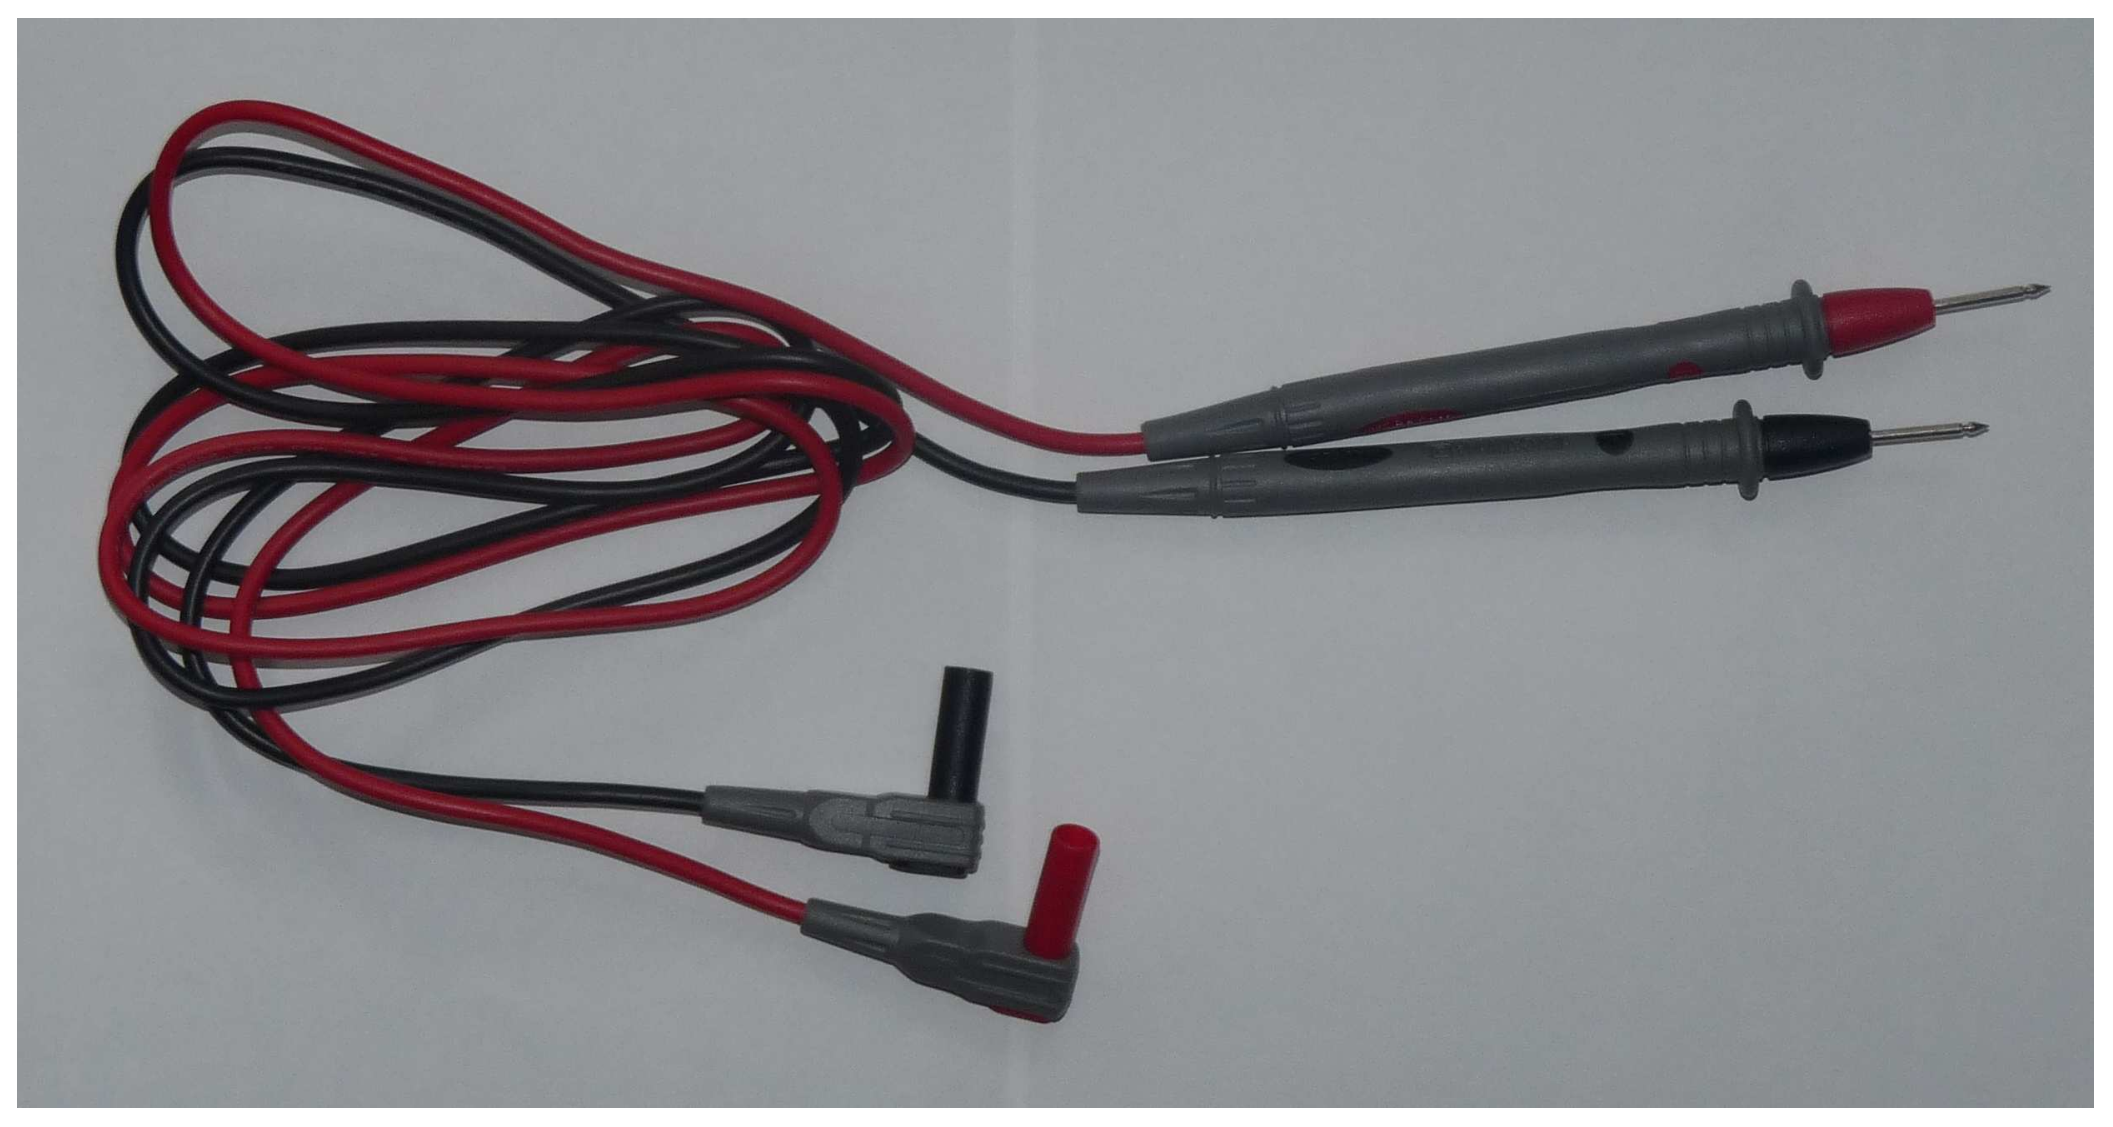
\includegraphics[width=\columnwidth]{modules/m0028_fMastech_test_leads.eps}
}}{Image of a set of electrical test leads. Each lead is comprised of a connector that fits the voltmeter and a tubular section with a pointed metal tip. The connector and metal probe tip are connected by wire. One lead is red and one is black.}
\end{center} 
%\vspace{2in}
% https://en.wikipedia.org/wiki/File:Mastech_test_leads.JPG
\centerline{\scriptsize 
by~\hyperref[m0028_fPoorTL_Credit]{Dmitry~G}
% public domain
}
\caption{
\label{m0028_fPoorTL}
These leads used to connect test equipment to circuits in a laboratory are a very rudimentary form of transmission line, suitable only for very low frequencies.
}
\end{figure}

However, many circuits and systems operate at frequencies where the length or cross-sectional dimensions of the transmission line may be a significant fraction of a wavelength. In this case, the transmission line is no longer ``transparent'' to the circuits at either end.
Furthermore, loss, reactance, and EMI \emph{are} significant problems in many applications.
These concerns motivate the use of particular types of transmission lines, and make it necessary to understand how to properly connect the transmission line to the rest of the system.

In electromagnetics, the term ``transmission line'' refers to a structure which is intended to support a \emph{guided wave}.
\index{waves!guided}
A guided wave is an electromagnetic wave that is contained within or bound to the line, and which does not radiate away from the line.  
This condition is normally met if the length and cross-sectional dimensions of the transmission line are small relative to a wavelength -- say $\lambda/100$ (i.e., 1\% of the wavelength). 
For example, two randomly-arranged wires might serve well enough to carry a signal at $f=10$~MHz over a length $l=3$~cm, since $l$ is only 0.1\% of the wavelength $\lambda=c/f=30$~m.  
However, if $l$ is increased to $3$~m, \emph{or} if $f$ is increased to 1~GHz, then $l$ is now 10\% of the wavelength.
In this case, one should consider using a transmission line that forms a proper guided wave. % that is not prone to unintended radiation. 

Preventing unintended radiation is not the only concern.
Once we have established a guided wave on a transmission line, it is important that power applied to the transmission line be delivered to the circuit or device at the other end and not reflected back into the source.
For the random wire $f=10$~MHz, $l=3$~cm example above, there is little need for concern, since we expect a phase shift of roughly $0.001\cdot 360^{\circ} = 0.36^{\circ}$ over the length of the transmission line, which is about $0.72^{\circ}$ for a round trip.  So, to a good approximation, the entire transmission line is at the same electrical potential and thus transparent to the source and destination.
However, if $l$ is increased to $3$~m, \emph{or} if $f$ is increased to 1~GHz, then the associated round-trip phase shift becomes $72^{\circ}$.  In this case, a reflected signal traveling in the opposite direction will add to create a total electrical potential, which varies in both magnitude and phase with position along the line. 
Thus, the impedance looking toward the destination via the transmission line will be different than the impedance looking toward the destination directly.
(Section~\ref{m0087_Input_Impedance_of_a_Terminated_Lossless_Transmission_Line} gives the details.)
The modified impedance will depend on the cross-sectional geometry, materials, and length of the line.  
     
Cross-sectional geometry and materials also determine the loss and EMI immunity of the transmission line.  

Summarizing:
%
%ORB HIGHLIGHT
\begin{mdframed}[backgroundcolor=yellow!20,nobreak=true] 
Transmission lines are designed to support guided waves with controlled impedance, low loss, and a degree of immunity from EMI. 
\end{mdframed}




      \vfill\break
    \section{Types of Transmission Lines}
{\color{blue}\tiny[m0144]}      % This is text associated with the open textbook "Open Electromagnetics"
% See immediately below for author, date
% This work is licensed under the Creative Commons Attribution-ShareAlike 4.0 International License. (CC BY-SA 4.0) 
% To view a copy of the license, visit http://creativecommons.org/licenses/by-sa/4.0/

%ORB TITLE Types of Transmission Lines
%ORB AUTHOR 0        # S.W. Ellingson, Virginia Tech (ellingson@vt.edu)
%ORB DATE 20180802   # yyyymmdd
%ORB ABSTRACT TEM vs. higher-order lines, quick overview of coax vs. microstrip vs. optical fiber etc.

\label{m0144_Types_of_Transmission_Lines} % <-- Must match name of this file and module directory name.  Don't mess with this!

Two common types of transmission line are
coaxial line 
\index{transmission line!coaxial}
\index{coax|see{transmission line}}
(Figure~\ref{m0028_fCoax}) and
microstrip line
\index{microstrip} 
(Figure~\ref{m0028_fMicrostrip}). 
Both are examples of \emph{transverse electromagnetic} (TEM) 
transmission lines.
A TEM line employs a single electromagnetic wave ``mode'' 
\index{mode}
having electric and magnetic field vectors in directions perpendicular to the axis of the line, as shown in Figures~\ref{m0144_fCoaxFieldStructure} and \ref{m0144_fMicrostripFieldStructure}.
%
TEM transmission lines appear primarily in radio frequency applications.
%
\begin{figure}[b!]
\begin{center}
\pdftooltip{{  % note double braces
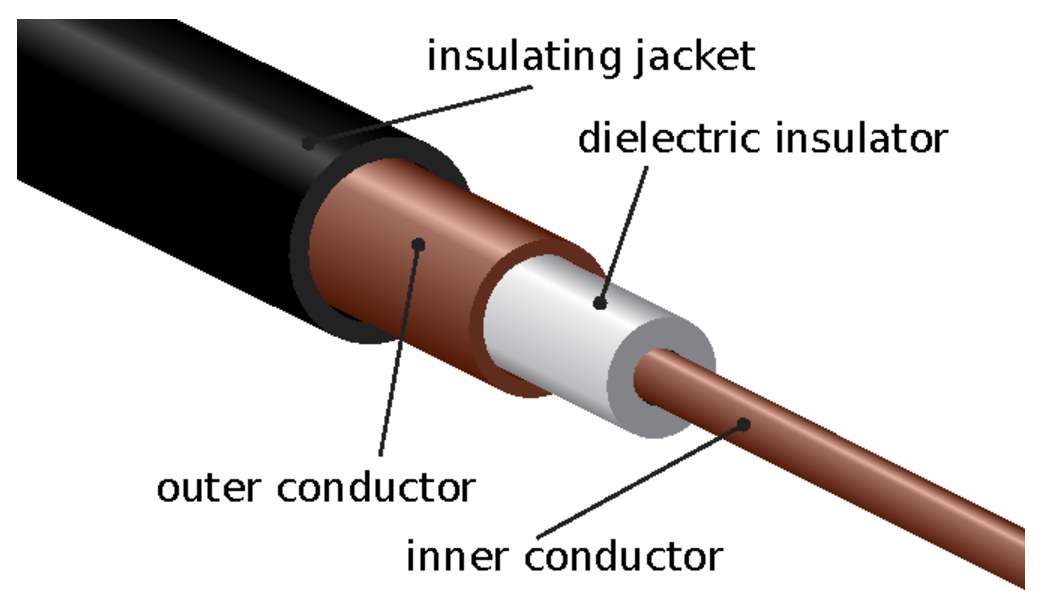
\includegraphics[width=2.5in]{modules/m0144_fCoaxial_cable_cutaway_170323se.eps}
% https://commons.wikimedia.org/wiki/File:Coaxial_cable_cutaway.svg
}}{The inner copper conductor wire is surrounded by a white dielectric insulator which is surrounded by an outer copper conductor layer which is surrounded by a black insulating jacket.}
\end{center} 
\centerline{\scriptsize 
\copyright~\hyperref[m0028_fCoax_Credit]{Tkgd2007} 
\href{https://creativecommons.org/licenses/by/3.0/}{CC BY 3.0} (modified)
} 
\caption{
\label{m0028_fCoax}
Structure of a coaxial transmission line. 
}
\end{figure}
%
\begin{figure}
\begin{center}
\pdftooltip{{  % note double braces
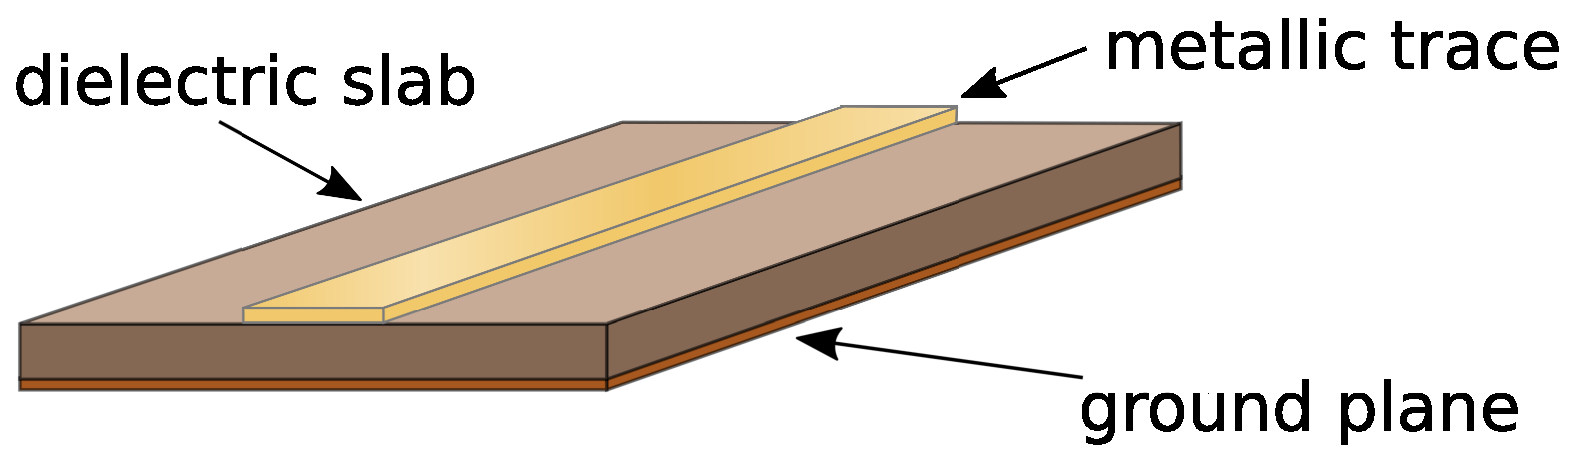
\includegraphics[width=2.5in]{modules/m0144_Microstrip_structure_170802se.eps}
% https://en.wikipedia.org/wiki/File:Microstrip_structure.svg
}}{A very thin, rectangular dielectric slab is set on the ground plane. Running longwise down the center of the dielectric slab is a thin layer of metallic trace.}
\end{center} 
\centerline{\scriptsize 
\copyright~\hyperref[m0028_fMicrostrip_Credit]{SpinningSpark} 
\href{https://creativecommons.org/licenses/by-sa/3.0/}{CC BY~SA 3.0} (modified)
} 
\caption{
\label{m0028_fMicrostrip}
Structure of a microstrip transmission line.
}
\end{figure}
%
\begin{figure}
\begin{center}
\pdftooltip{{  % note double braces
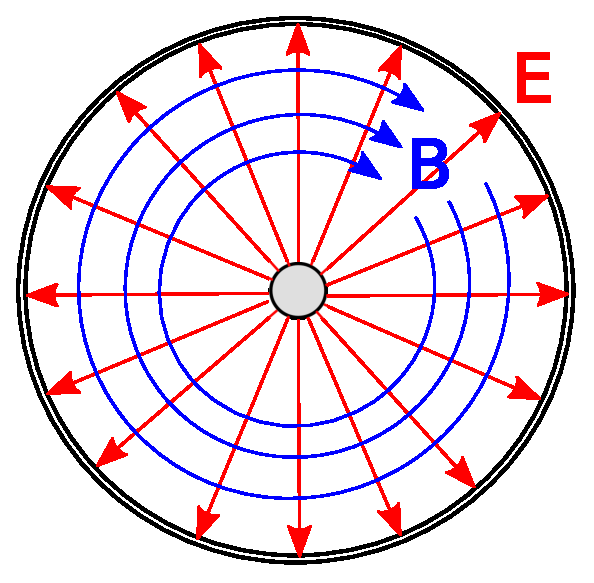
\includegraphics[width=1.5in]{modules/m0144_fCoaxFieldStructure.eps}
}}{A cross-sectional view of a coaxial transmission line. The inner conductor is represented by a gray-filled circle.  The electric field, "E", is represented by red arrows pointing outward from the inner conductor to the outer conductor which is represented by a larger concentric circle. The magnetic field, "B" is represented by concentric, circular blue arrows between the insulating jacket and the inner conductor. The arrows indicate a clockwise direction.}
\end{center} 
%\vspace{2.5in}
\caption{\label{m0144_fCoaxFieldStructure}Structure of the electric and magnetic fields within coaxial line.  In this case, the wave is propagating away from the viewer.}
\end{figure}
%
\begin{figure}
\begin{center}
\pdftooltip{{  % note double brace
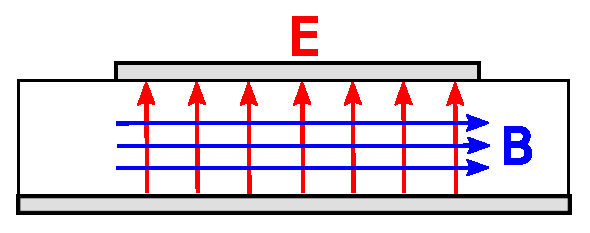
\includegraphics[width=2.0in]{modules/m0144_fMicrostripFieldStructure.eps}
}}{A cross-sectional view of a microstrip line. The electric field "E" is represented by a row of red parallel arrows pointing vertically from the ground plane to the metallic trace. The magnetic field "B" is represented by parallel blue arrows perpendicular to the electric field arrows, pointing to the right.}
\end{center} 
%\vspace{2.5in}
\caption{\label{m0144_fMicrostripFieldStructure}Structure of the electric and magnetic fields within microstrip line. (The fields \emph{outside} the line are possibly significant, complicated, and not shown.)  In this case, the wave is propagating away from the viewer.}
\end{figure}

%ORB HIGHLIGHT
\begin{mdframed}[backgroundcolor=yellow!20,nobreak=true] 
TEM transmission lines 
\index{transmission line!transverse electromagnetic (TEM)}
\index{TEM line|see{transmission line}}
such as coaxial lines and microstrip lines are designed to support a single electromagnetic wave that propagates along the length of the transmission line with electric and magnetic field vectors perpendicular to the direction of propagation.
\end{mdframed}

Not all transmission lines exhibit TEM field structure.
In non-TEM transmission lines, the electric and magnetic field vectors that are not necessarily perpendicular to the axis of the line, and the structure of the fields is complex relative to the field structure of TEM lines. 
An example of a transmission line that exhibits non-TEM field structure is the waveguide 
\index{waveguide}
(see example in Figure~\ref{m0028_fWaveGuide}).
Waveguides are most prevalent at radio frequencies, and tend to appear in applications where it is important to achieve very low loss or where power levels are very high.
Another example is common ``multimode'' optical fiber (Figure~\ref{m0028_fOpticalFiber}).
\index{optical fiber!multimode}
Optical fiber exhibits complex field structure because the wavelength of light is very small compared to the cross-section of the fiber, making the excitation and propagation of non-TEM waves difficult to avoid. (This issue is overcome in a different type of optical fiber, known as ``single mode'' fiber, 
\index{optical fiber!single mode}
which is much more difficult and expensive to manufacture.)  
%(Transmission lines for frequencies in the UV band and higher are not commonly encountered.)
%
\begin{figure}
\begin{center}
\pdftooltip{{  % note double braces
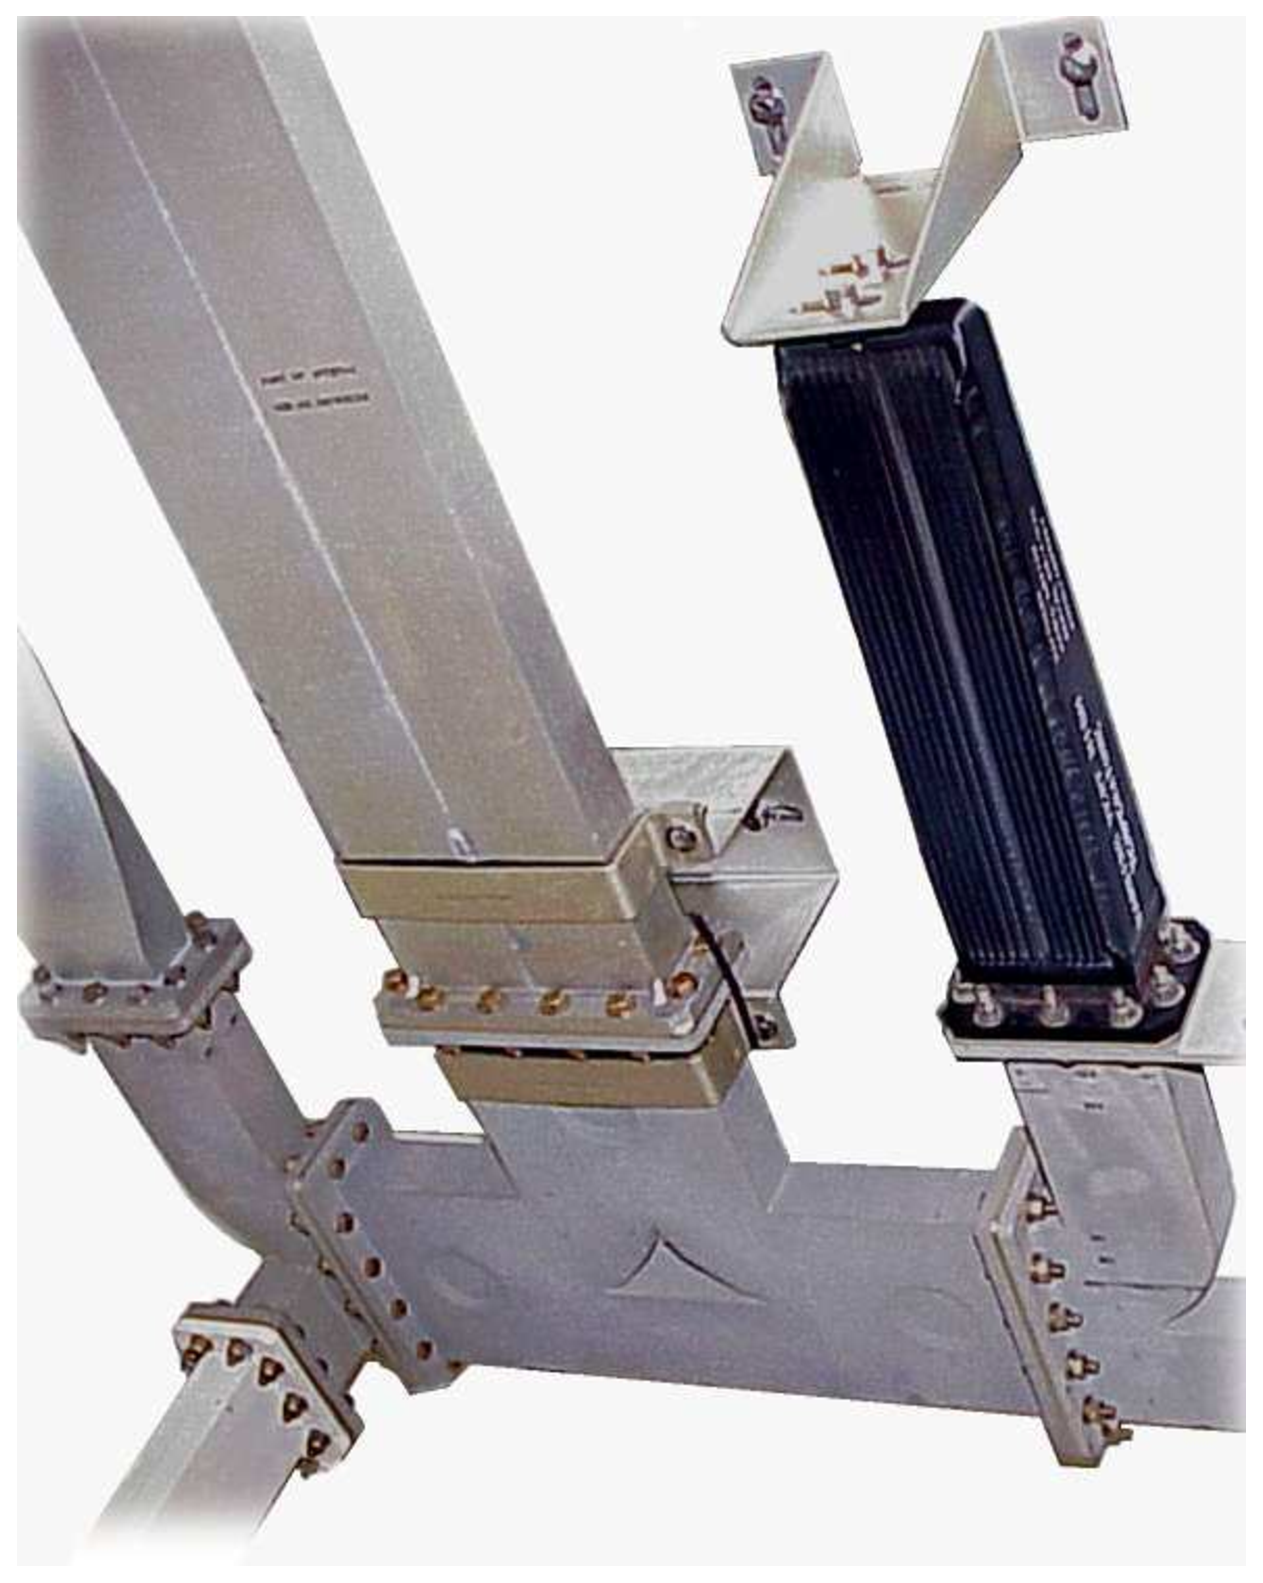
\includegraphics[width=2.5in]{modules/m0144_fDiplexer1.eps}
% https://en.wikipedia.org/wiki/File:Diplexer1.jpg
}}{Photo of waveguide highlighting multiple branching connections running in parallel.}
\end{center} 
\centerline{\scriptsize 
\copyright~\hyperref[m0028_fWaveGuide_Credit]{Averse} 
\href{https://creativecommons.org/licenses/by-sa/2.0/de/deed.en}{CC BY~SA 2.0 Germany} 
} 
\caption{
\label{m0028_fWaveGuide}
A network of radio frequency waveguides in an air traffic control radar.
}
\end{figure}
%
\begin{figure}
\begin{center}
\pdftooltip{{  % note double braces
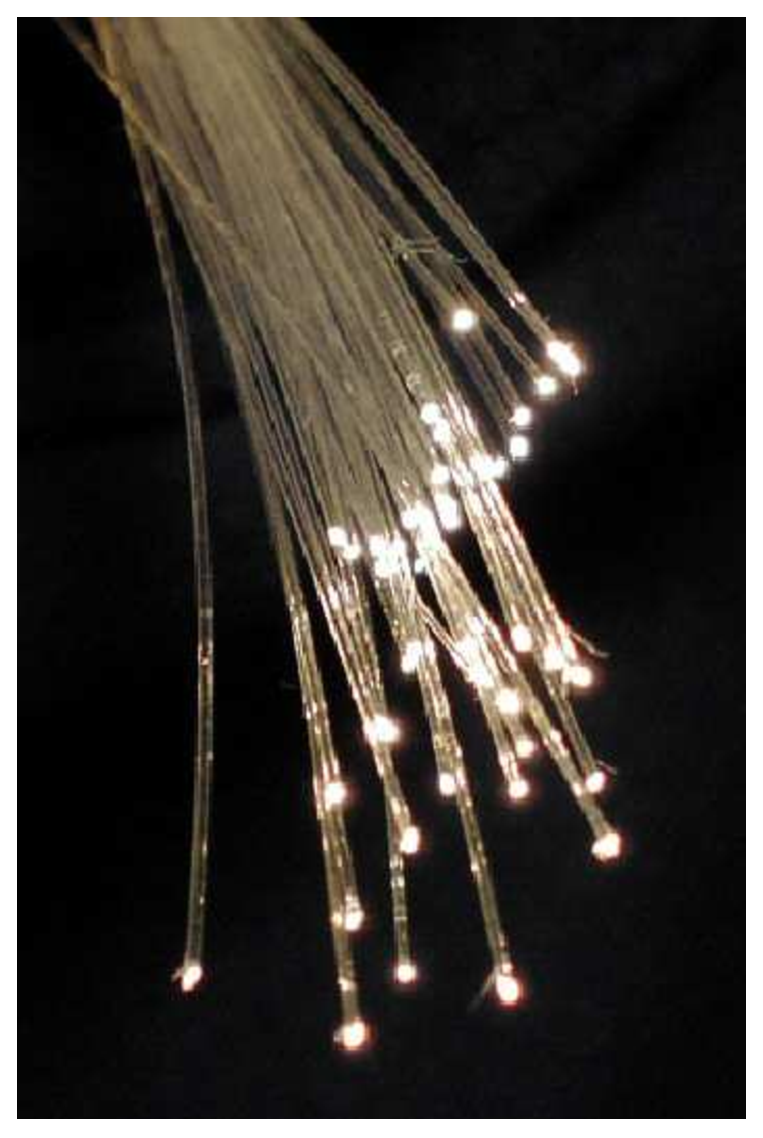
\includegraphics[width=1.5in]{modules/m0144_fFibreoptic.eps}
% https://en.wikipedia.org/wiki/File:Fibreoptic.jpg
}}{A bundle of clear, thin strands of fiber in a dark background. The tips of the fibers are glowing with white light.}
\end{center} 
\centerline{\scriptsize 
\copyright~\hyperref[m0028_fOpticalFiber_Credit]{BigRiz} 
\href{https://creativecommons.org/licenses/by-sa/3.0/deed.en}{CC BY~SA 3.0 Unported} 
} 
\caption{
\label{m0028_fOpticalFiber}
Strands of optical fiber.
}
\end{figure}

%ORB HIGHLIGHT
\begin{mdframed}[backgroundcolor=yellow!20,nobreak=true] 
Higher-order transmission lines, including radio-frequency waveguides and multimode optical fiber, are designed to guide waves that have relatively complex structure.
\end{mdframed}

%%%%%%%%%%%%%%%%%%%%%%%%%%%%%%%%%

{\bf Additional Reading:}
\begin{itemize}
\item ``\href{https://en.wikipedia.org/wiki/Coaxial_cable}{Coaxial cable}'' on Wikipedia.
\item ``\href{https://en.wikipedia.org/wiki/Microstrip}{Microstrip}'' on Wikipedia.
\item ``\href{https://en.wikipedia.org/wiki/Waveguide_(electromagnetism)}{Waveguide (electromagnetism)}'' on Wikipedia.
\item ``\href{https://en.wikipedia.org/wiki/Optical_fiber}{Optical fiber}'' on Wikipedia.
\end{itemize}

       


      \vfill\break
    \section{Transmission Lines as Two-Port Devices}
{\color{blue}\tiny[m0077]}      % This is text associated with the open textbook "Open Electromagnetics"
% See immediately below for author, date
% This work is licensed under the Creative Commons Attribution-ShareAlike 4.0 International License. (CC BY-SA 4.0) 
% To view a copy of the license, visit http://creativecommons.org/licenses/by-sa/4.0/

%ORB TITLE Transmission Lines as Two-Port Devices
%ORB AUTHOR 0        # S.W. Ellingson, Virginia Tech (ellingson@vt.edu)
%ORB DATE 20180802   # yyyymmdd
%ORB ABSTRACT Transmission Lines as Two-Ports

\label{m0077_Transmission_Lines_as_Two-Ports} % <-- Must match name of this file and module directory name.  Don't mess with this!
\index{transmission line!two-port representation|(}

Figure~\ref{m0077_fTransmission_line_symbols} shows common ways to represent transmission lines in circuit diagrams.
In each case, the source is represented using a Th\'{e}venin equivalent circuit 
\index{Th\'{e}venin equivalent circuit}
consisting of a voltage source $V_S$ in series with an impedance $Z_S$.\footnote{For a refresher on this concept, see ``Additional Reading'' at the end of this section.}  In transmission line analysis, the source may also be referred to as the \emph{generator}.
\index{generator}
The termination on the receiving end of the transmission line is represented, without loss of generality, as an impedance $Z_L$. 
This termination is often referred to as the \emph{load}, although in practice it can be any circuit that exhibits an input impedance of $Z_L$.
%
\begin{figure}[b!]
\begin{center}
\pdftooltip{{  % note double braces
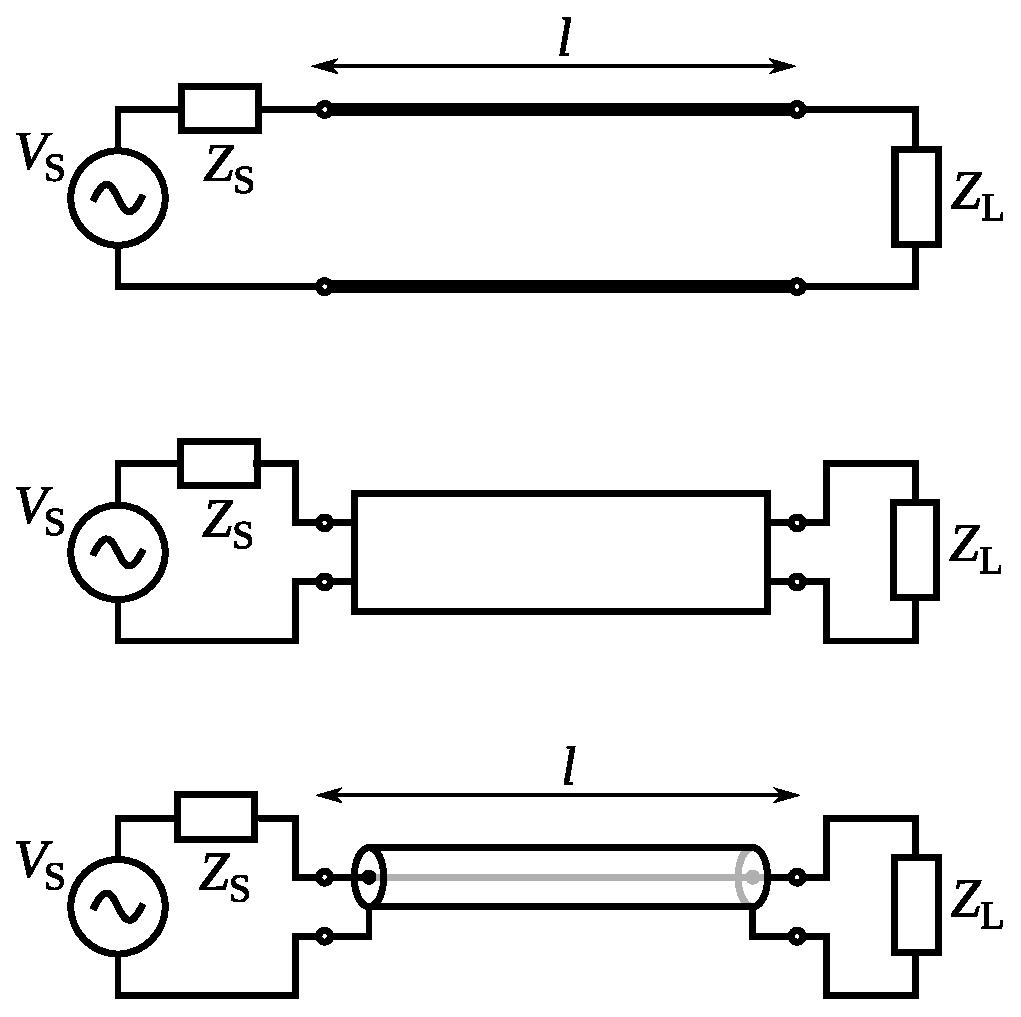
\includegraphics[width=\columnwidth]{modules/m0077_Transmission_line_symbols_se170804.eps}
% https://commons.wikimedia.org/wiki/File:Transmission_line_symbols.svg
}}{Three circuit diagrams depicting a generic two-conductor direct connection (top), a generic two port "black box" (middle), and a coaxial cable (bottom). The top diagram consists of a rectangular series circuit with a circle with a curved line in it representing the voltage source (V sub s) on the left. A source impedance (Z sub s) is represented by a small rectangle to the right of source. A load impedance (Z sub L) is represented by a small rectangle on the right side of the circuit. V sub s, Z sub s, and Z sub L are identically placed in the other two diagrams. On the top and bottom of the rectangle, a thicker line labeled "l" represents the length of the transmission line.  The middle diagram shows another rectangle laid over the middle of the circuit representing a two-port "black box." The bottom diagram depicts a cylinder laid over the middle of the circuit, with the circuit going through it, to represent a coaxial cable.}
\end{center} 
\centerline{\scriptsize 
\copyright~\hyperref[m0077_fTransmission_line_symbols_Credit]{Omegatron}
\href{https://creativecommons.org/licenses/by-sa/3.0/deed.en}{CC BY~SA 3.0 Unported} (modified) 
} 
\caption{
\label{m0077_fTransmission_line_symbols}
Symbols representing transmission lines: 
\emph{Top}: As a generic two-conductor direct connection.
\emph{Middle}: As a generic two-port ``black box.''
\emph{Bottom}: As a coaxial cable. 
}
\end{figure}

The two-port representation
\index{two-port}
of a transmission line is completely described by its length $l$ along with some combination of the following parameters: 
%
\begin{itemize}
\item Phase propagation constant $\beta$, 
\index{propagation constant!phase}
having units of rad/m.  This parameter also represents the wavelength in the line through the relationship $\lambda=2\pi/\beta$.
(See Sections~\ref{m0074_Fundamentals_of_Waves} and \ref{m0080_Wave_Propagation_on_a_Transmission_Line} for details.)
\item Attenuation constant $\alpha$, 
\index{propagation constant!attenuation}
having units of 1/m. This parameter quantifies the effect of loss in the line.
(See Section~\ref{m0080_Wave_Propagation_on_a_Transmission_Line} for details.)
\item Characteristic impedance $Z_0$, 
\index{characteristic impedance}
\index{impedance!characteristic|see{characteristic impedance}}
having units of $\Omega$.  This is the ratio of potential (``voltage'') to current when the line is perfectly impedance-matched at both ends.
(See Section~\ref{m0052_Characteristic_Impedance} for details.)  
\end{itemize}
These parameters depend on the materials and geometry of the line.

Note that a transmission line is typically not transparent to the source and load.
In particular, the load impedance may be $Z_L$, but the impedance presented to the source may or may not be equal to $Z_L$.
(See Section~\ref{m0087_Input_Impedance_of_a_Terminated_Lossless_Transmission_Line} for more on this concept.)
Similarly, the source impedance may be $Z_S$, but the impedance presented to the load may or may not be equal to $Z_S$.
The effect of the transmission line on the source and load impedances will depend on the parameters identified above.

%%%%%%%%%%%%%%%%%%%%%%%%%%%%%%%%

{\bf Additional Reading:}
\begin{itemize}
\item ``\href{https://en.wikipedia.org/wiki/Thevenin's_theorem}{Th\'{e}venin's theorem}'' on Wikipedia.
\end{itemize}

\index{transmission line!two-port representation|)}


      \vfill\break
    \section{Lumped-Element Model}
{\color{blue}\tiny[m0029]}      % This is text associated with the open textbook "Open Electromagnetics"
% See immediately below for author, date
% This work is licensed under the Creative Commons Attribution-ShareAlike 4.0 International License. (CC BY-SA 4.0) 
% To view a copy of the license, visit http://creativecommons.org/licenses/by-sa/4.0/

%ORB TITLE Lumped-Element Model
%ORB AUTHOR 0        # S.W. Ellingson, Virginia Tech (ellingson@vt.edu)
%ORB DATE 20180802  # yyyymmdd
%ORB ABSTRACT Lumped-element model of transmission line, leading the telegrapher's equations 

\label{m0029_Lumped-Element_Model} % <-- Must match name of this file and module directory name.  Don't mess with this!
\index{transmission line!lumped-element model|(}
\index{lumped-element model|see{transmission line}}

It is possible to ascertain the relevant behaviors of a transmission line using elementary circuit theory applied to a differential-length lumped-element model of the transmission line.
The concept is illustrated in Figure~\ref{m0029_fTL_to_differential_segments}, which shows a generic transmission line aligned with its length along the $z$ axis.
The transmission line is divided into segments having small but finite length $\Delta z$.
Each segment is modeled as an identical two-port having the equivalent circuit representation shown in Figure~\ref{m0029_fLumpedElementModel}.
The equivalent circuit consists of 4 components as follows:
%
\begin{itemize}
\item  The resistance 
\index{resistance}
$R'\Delta z$ represents the series-combined ohmic resistance of the two conductors.  This should account for {\it both} conductors since the current in the actual transmission line must flow through both conductors.  The prime notation reminds us that $R'$ is resistance \emph{per unit length}; i.e., $\Omega$/m, and it is only after multiplying by length that we get a resistance in $\Omega$. 
\item  The conductance 
\index{conductance}
$G'\Delta z$ represents the leakage of current directly from one conductor to the other.
When $G'\Delta z>0$, the resistance between the conductors is less than infinite, and therefore, current may flow between the conductors.  
This amounts to a loss of power separate from the loss associated with $R'$ above.  $G'$ has units of S/m.  Further note that $G'$ is \emph{not} equal to $1/R'$ as defined above. $G'$ and $R'$ are describing entirely different physical mechanisms (and in principle \emph{either} could be defined as either a resistance or a conductance).
\item  The capacitance 
\index{capacitance}
$C'\Delta z$ represents the capacitance of the transmission line structure.  Capacitance is the tendency to store energy in electric fields and depends on the cross-sectional geometry and the media separating the conductors. $C'$ has units of F/m.
\item The inductance
\index{inductance}
$L'\Delta z$ represents the inductance of the transmission line structure.  Inductance is the tendency to store energy in magnetic fields, and (like capacitance) depends on the cross-sectional geometry and the media separating the conductors.
$L'$ has units of H/m.
\end{itemize}  
%
\begin{figure}
\begin{center}
\pdftooltip{{  % note double braces
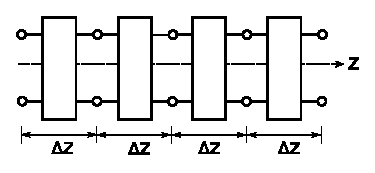
\includegraphics[width=2.5in]{modules/m0029_fTL_to_differential_segments.eps}
}}{Four rectangles arranged in a horizontal line intersected in the middle by a dashed arrow pointing to the right labeled z. The 2 nodes of each rectangle are shown joining the next rectangle to the right. The distance from node to node horizontally is Delta z.}
\end{center} 
\caption{\label{m0029_fTL_to_differential_segments}
Interpretation of a transmission line as a cascade of discrete series-connected two-ports.}
\end{figure}
%
\begin{figure}
\begin{center}
\pdftooltip{{  % note double braces
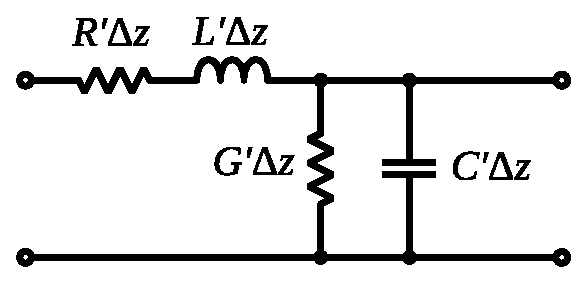
\includegraphics[width=2in]{modules/m0029_Transmission_line_element_se170804.eps}
}}{From left to right, a resistor and inductor in series then connected to a resistor and capacitor in parallel. The left (series) resistor is labeled R' Delta z. 
The inductor is labeled L' Delta z. On the left vertical line, a resistor symbol represents G’ Delta z. On the right vertical line, a capacitor symbol represents C Delta z.}
\end{center} 
%\vspace{2in}
% https://commons.wikimedia.org/wiki/File:Transmission_line_element.svg
\centerline{\scriptsize 
\copyright~\hyperref[m0029_fLumpedElementModel_Credit]{Omegatron} 
\href{https://creativecommons.org/licenses/by-sa/3.0/deed.en}{CC BY~SA 3.0 Unported} (modified) 
} 
\caption{
\label{m0029_fLumpedElementModel}
Lumped-element equivalent circuit model for each of the two-ports in Figure~\ref{m0029_fTL_to_differential_segments}.
}
\end{figure}

In order to use the model, one must have values for $R'$, $G'$, $C'$, and $L'$.   
Methods for computing these parameters are addressed elsewhere in this book. 

\index{transmission line!lumped-element model|)}


      \vfill\break
    \section{Telegrapher's Equations}
{\color{blue}\tiny[m0079]}      % This is text associated with the open textbook "Open Electromagnetics"
% See immediately below for author, date
% This work is licensed under the Creative Commons Attribution-ShareAlike 4.0 International License. (CC BY-SA 4.0) 
% To view a copy of the license, visit http://creativecommons.org/licenses/by-sa/4.0/

%ORB TITLE Telegrapher's Equations
%ORB AUTHOR 0        # S.W. Ellingson, Virginia Tech (ellingson@vt.edu)
%ORB DATE 20180802   # yyyymmdd
%ORB ABSTRACT Development of the telegrapher's equations given the lumped-element model.

\label{m0079_Telegraphers_Equations} % <-- Must match name of this file and module directory name.  Don't mess with this!
\index{telegrapher's equations|(}

In this section, we derive the equations that govern the potential $v(z,t)$ and current $i(z,t)$ along a transmission line that is oriented along the $z$ axis.  
For this, we will employ the lumped-element model developed in Section~\ref{m0029_Lumped-Element_Model}.

To begin, we define voltages and currents as shown in Figure~\ref{m0079_fLumpedElementModel}.  
%
\begin{figure}[b!]
\begin{center}
\pdftooltip{{  % note double brace
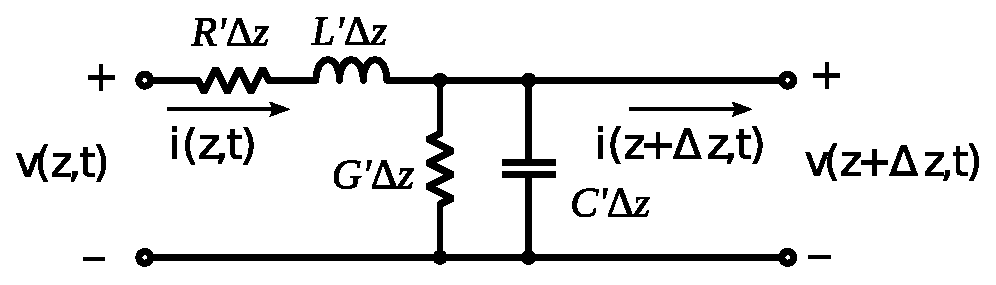
\includegraphics[width=\columnwidth]{modules/m0079_Transmission_line_element_se170804.eps}
% https://commons.wikimedia.org/wiki/File:Transmission_line_element.svg (modified)
}}{A lumped-element equivalent circuit model the same as an earlier figure. On the left side open node, the potential v(z,t) is shown with positive terminal applied to the resistor.  Underneath the series resistor, a right pointing arrow is labeled i(z,t). On the right side of the circuit, the voltage potential is given as v( z + Delta z, t ). On the positive exit node, an arrow labeled i( z + Delta z, t ) points to the right.}
\end{center} 
\centerline{\scriptsize 
\copyright~\hyperref[m0079_fLumpedElementModel_Credit]{Omegatron} 
\href{https://creativecommons.org/licenses/by-sa/3.0/deed.en}{CC BY~SA 3.0 Unported} (modified) 
} 
\caption{
\label{m0079_fLumpedElementModel}
Lumped-element equivalent circuit transmission line model, annotated with sign conventions for potentials and currents.
}
\end{figure}
%
We assign the variables $v(z,t)$ and $i(z,t)$ to represent the potential and current on the left side of the segment, with reference polarity and direction as shown in the figure.
Similarly we assign the variables $v(z+\Delta z,t)$ and $i(z+\Delta z,t)$ to represent the potential and current on the right side of the segment, again with reference polarity and direction as shown in the figure.
Applying Kirchoff's voltage law from the left port, through $R'\Delta z$ and $L'\Delta z$, and returning via the right port, we obtain:
%
\begin{multline}
v(z,t) - \left( R'\Delta z \right) i(z,t) - \left( L' \Delta z\right) \frac{\partial}{\partial t} i(z,t) \\ - v(z+\Delta z,t) = 0
\end{multline}
%
Moving terms referring to current to the right side of the equation and then dividing through by $\Delta z$, we obtain
%
\begin{multline}
-\frac{v(z+\Delta z,t)-v(z,t)}{\Delta z} = \\
R'~i(z,t) + L'~\frac{\partial}{\partial t} i(z,t)
\end{multline}
%
Then taking the limit as $\Delta z \rightarrow 0$:
%
\begin{multline}
\boxed{
-\frac{\partial}{\partial z} v(z,t) = 
R'~i(z,t) + L'~\frac{\partial}{\partial t} i(z,t)
}
\label{m0079_eTelegraphersEquation1}
\end{multline}

Applying Kirchoff's current law at the right port, we obtain:
%
\begin{multline}
i(z,t) - \left( G'\Delta z \right) v(z+\Delta z,t) - \left( C' \Delta z\right) \frac{\partial}{\partial t} v(z+\Delta z,t) \\ - i(z+\Delta z,t) = 0
\end{multline}
%
Moving terms referring to potential to the right side of the equation and then dividing through by $\Delta z$, we obtain
%
\begin{multline}
-\frac{i(z+\Delta z,t)-i(z,t)}{\Delta z} = \\
G'~v(z+\Delta z,t) + C'~\frac{\partial}{\partial t} v(z+\Delta z,t)
\end{multline}
%
Taking the limit as $\Delta z \rightarrow 0$:
%
\begin{multline}
\boxed{
-\frac{\partial}{\partial z} i(z,t) = 
G'~v(z,t) + C'~\frac{\partial}{\partial t} v(z,t)
}
\label{m0079_eTelegraphersEquation2}
\end{multline}
%
%ORB HIGHLIGHT
\begin{mdframed}[backgroundcolor=yellow!20,nobreak=true] 
Equations~\ref{m0079_eTelegraphersEquation1} and \ref{m0079_eTelegraphersEquation2} are the \emph{telegrapher's equations}.  These coupled (simultaneous) differential equations can be solved for $v(z,t)$ and $i(z,t)$ given $R'$, $G'$, $L'$, $C'$ and suitable boundary conditions.
\end{mdframed}

The time-domain telegrapher's equations are usually more than we need or want.  If we are only interested in the response to a sinusoidal stimulus, then considerable simplification is possible using phasor representation.\footnote{For a refresher on phasor analysis, see Section~\ref{m0033_Phasors}.}  First we define phasors $\widetilde{V}(z)$ and $\widetilde{I}(z)$ through the usual relationship:
%
\begin{equation}
v(z,t) = \mbox{Re}\left\{\widetilde{V}(z) ~ e^{j\omega t} \right\}
\end{equation}
%
\begin{equation}
i(z,t) = \mbox{Re}\left\{\widetilde{I}(z) ~ e^{j\omega t} \right\}
\end{equation}  
%
Now we see:
%
\begin{equation}
\begin{split}
\frac{\partial}{\partial z} v(z,t) & = \frac{\partial}{\partial z} \mbox{Re}\left\{\widetilde{V}(z) ~ e^{j\omega t} \right\} \nonumber \\
                                   & = \mbox{Re}\left\{ \left[ \frac{\partial}{\partial z} \widetilde{V}(z) \right] ~ e^{j\omega t} \right\}
\end{split}
\end{equation}
%
In other words, $\partial v(z,t)/\partial z$ expressed in phasor representation is simply $\partial \widetilde{V}(z)/\partial z$; and 
%
\begin{equation}
\begin{split}
\frac{\partial}{\partial t} i(z,t) & = \frac{\partial}{\partial t} \mbox{Re}\left\{\widetilde{I}(z) ~ e^{j\omega t} \right\} \nonumber \\
                                   & = \mbox{Re}\left\{ \frac{\partial}{\partial t} \left[ \widetilde{I}(z) e^{j\omega t} \right] \right\} \nonumber \\
                                   & = \mbox{Re}\left\{ \left[ j\omega \widetilde{I}(z) \right] e^{j\omega t} \right\}
\end{split}
\end{equation}
%
In other words, $\partial i(z,t)/\partial t$ expressed in phasor representation is $j\omega \widetilde{I}(z)$.
Therefore, Equation~\ref{m0079_eTelegraphersEquation1} expressed in phasor representation is:
%
\begin{equation}
\boxed{
-\frac{\partial}{\partial z} \widetilde{V}(z) = \left[ R' + j\omega L' \right]~\widetilde{I}(z)
}
\label{m0079_eTelegraphersEquation1p}
\end{equation}
%
Following the same procedure, Equation~\ref{m0079_eTelegraphersEquation2} expressed in phasor representation is found to be:
%
\begin{equation}
\boxed{
-\frac{\partial}{\partial z} \widetilde{I}(z) = \left[ G' + j\omega C' \right]~\widetilde{V}(z)
}
\label{m0079_eTelegraphersEquation2p}
\end{equation}
%
%ORB HIGHLIGHT
\begin{mdframed}[backgroundcolor=yellow!20,nobreak=true] 
Equations~\ref{m0079_eTelegraphersEquation1p} and \ref{m0079_eTelegraphersEquation2p} are the telegrapher's equations in phasor representation. 
\end{mdframed}
%
The principal advantage of these equations over the time-domain versions is that we no longer need to contend with derivatives with respect to time -- only derivatives with respect to distance remain.
This considerably simplifies the equations.

%%%%%%%%%%%%%%%%%%%%%%%%%%%%%%%%%%%%%%%%%%%

{\bf Additional Reading:}
\begin{itemize}
\item ``\href{https://en.wikipedia.org/wiki/Telegrapher's_equations}{Telegrapher's equations}'' on Wikipedia.
\item ``\href{https://en.wikipedia.org/wiki/Kirchhoff's_circuit_laws}{Kirchhoff's circuit laws}'' on Wikipedia.
\end{itemize}

\index{telegrapher's equations|)}





      \vfill\break
    \section{Wave Equation for a TEM Transmission Line}
{\color{blue}\tiny[m0027]}      % This is text associated with the open textbook "Open Electromagnetics"
% See immediately below for author, date
% This work is licensed under the Creative Commons Attribution-ShareAlike 4.0 International License. (CC BY-SA 4.0) 
% To view a copy of the license, visit http://creativecommons.org/licenses/by-sa/4.0/

%ORB TITLE Wave Equation for a TEM Transmission Line
%ORB AUTHOR 0        # S.W. Ellingson, Virginia Tech (ellingson@vt.edu)
%ORB DATE 20180802   # yyyymmdd
%ORB ABSTRACT Beginning with phasor Telegrapher's equations, obtain wave equations for V(z) and I(z)

\label{m0027_Wave_Equations_for_a_Transmission_Line} % <-- Must match name of this file and module directory name.  Don't mess with this!
\index{wave equation!TEM transmission line|(}
\index{transmission line!wave equations|(}

Consider a TEM transmission line 
\index{transmission line!transverse electromagnetic (TEM)}
aligned along the $z$ axis.
The phasor form of the Telegrapher's Equations 
\index{telegrapher's equations}
(Section~\ref{m0079_Telegraphers_Equations}) relate the potential phasor
$\widetilde{V}(z)$ and the current phasor $\widetilde{I}(z)$ to each other and 
to the lumped-element model equivalent circuit parameters $R'$, $G'$, $C'$, and $L'$.
These equations are
%
\begin{equation}
-\frac{\partial}{\partial z} \widetilde{V}(z) = \left[ R' + j\omega L' \right]~\widetilde{I}(z)
\label{m0027_eTelegraphersEquation1p}
\end{equation}
%
\begin{equation}
-\frac{\partial}{\partial z} \widetilde{I}(z) = \left[ G' + j\omega C' \right]~\widetilde{V}(z)
\label{m0027_eTelegraphersEquation2p}
\end{equation}

An obstacle to using these equations is that we require both equations to solve for either the potential or the current.
In this section, we reduce these equations to a single equation -- a \emph{wave equation} -- that is more convenient to use and provides some additional physical insight.

We begin by differentiating both sides of Equation~\ref{m0027_eTelegraphersEquation1p} with respect to $z$, yielding:
%
\begin{equation}
-\frac{\partial^2}{\partial z^2} \widetilde{V}(z) = \left[ R' + j\omega L' \right]~\frac{\partial}{\partial z} \widetilde{I}(z)
\end{equation}
%
Then using Equation~\ref{m0027_eTelegraphersEquation2p} to eliminate $\widetilde{I}(z)$, we obtain
%
\begin{equation}
-\frac{\partial^2}{\partial z^2} \widetilde{V}(z) = -\left[ R' + j\omega L' \right]\left[ G' + j\omega C' \right]~\widetilde{V}(z)
\end{equation}
%
This equation is normally written as follows:
%
\begin{equation}
\boxed{
\frac{\partial^2}{\partial z^2} \widetilde{V}(z) -\gamma^2~\widetilde{V}(z) =0
}
\label{m0027_eWaveEqnV}
\end{equation}
%
where we have made the substitution:
%
\begin{equation}
\gamma^2 = \left( R' + j\omega L' \right)\left( G' + j\omega C' \right)
\end{equation}
%
The principal square root of $\gamma^2$ is known as the \emph{propagation constant}:
%
\begin{equation}
\gamma \triangleq \sqrt{\left( R' + j\omega L' \right)\left( G' + j\omega C' \right)} 
\label{m0027_egamma}
\end{equation}
%
%ORB HIGHLIGHT
\begin{mdframed}[backgroundcolor=yellow!20,nobreak=true] 
The \emph{propagation constant} 
\index{propagation constant}
$\gamma$ (units of m$^{-1}$) captures the effect of materials, geometry, and frequency in determining the variation in potential and current with distance on a TEM transmission line. 
\end{mdframed}

Following essentially the same procedure but beginning with Equation~\ref{m0027_eTelegraphersEquation2p}, we obtain
%
\begin{equation}
\boxed{
\frac{\partial^2}{\partial z^2} \widetilde{I}(z) -\gamma^2~\widetilde{I}(z) =0
}
\label{m0027_eWaveEqnI}
\end{equation}
%
%ORB HIGHLIGHT
\begin{mdframed}[backgroundcolor=yellow!20,nobreak=true] 
Equations~\ref{m0027_eWaveEqnV} and \ref{m0027_eWaveEqnI} are the \emph{wave equations} for $\widetilde{V}(z)$ and $\widetilde{I}(z)$, respectively.
\end{mdframed}

Note that both $\widetilde{V}(z)$ and $\widetilde{I}(z)$ satisfy the \emph{same} linear homogeneous differential equation.
This does \emph{not} mean that $\widetilde{V}(z)$ and $\widetilde{I}(z)$ are equal.
Rather, it means that $\widetilde{V}(z)$ and $\widetilde{I}(z)$ can differ by no more than a multiplicative constant.
Since $\widetilde{V}(z)$ is potential and $\widetilde{I}(z)$ is current, that constant must be an impedance.
This impedance is known as the \emph{characteristic impedance} 
\index{characteristic impedance}
and is determined in Section~\ref{m0052_Characteristic_Impedance}.

The general solutions to Equations~\ref{m0027_eWaveEqnV} and \ref{m0027_eWaveEqnI} are
%
\begin{equation}
\widetilde{V}(z) = V_0^+ e^{-\gamma z} + V_0^- e^{+\gamma z}
\label{m0027_eV}
\end{equation}
%
\begin{equation}
\widetilde{I}(z) = I_0^+ e^{-\gamma z} + I_0^- e^{+\gamma z}
\label{m0027_eI}
\end{equation}
%
where $V_0^+$, $V_0^-$, $I_0^+$, and $I_0^-$ are complex-valued constants.
It is shown in Section~\ref{m0080_Wave_Propagation_on_a_Transmission_Line} that Equations~\ref{m0027_eV} and \ref{m0027_eI} represent sinusoidal waves propagating in the $+z$ and $-z$ directions along the length of the line.
The constants may represent sources, loads, or simply discontinuities in the materials and/or geometry of the line.
The values of the constants are determined by boundary conditions; i.e., constraints on $\widetilde{V}(z)$ and $\widetilde{I}(z)$ at some position(s) along the line.  

The reader is encouraged to verify that the Equations~\ref{m0027_eV} and \ref{m0027_eI} are in fact solutions to Equations~\ref{m0027_eWaveEqnV} and \ref{m0027_eWaveEqnI}, respectively, for any values of the constants $V_0^+$, $V_0^-$, $I_0^+$, and $I_0^-$.

\index{wave equation!TEM transmission line|)}
\index{transmission line!wave equations|)}


      \vfill\break
    \section{Characteristic Impedance}
{\color{blue}\tiny[m0052]}      % This is text associated with the open textbook "Open Electromagnetics"
% See immediately below for author, date
% This work is licensed under the Creative Commons Attribution-ShareAlike 4.0 International License. (CC BY-SA 4.0) 
% To view a copy of the license, visit http://creativecommons.org/licenses/by-sa/4.0/

%ORB TITLE Characteristic Impedance
%ORB AUTHOR 0        # S.W. Ellingson, Virginia Tech (ellingson@vt.edu)
%ORB DATE 20180802   # yyyymmdd
%ORB ABSTRACT Characteristic Impedance

\label{m0052_Characteristic_Impedance} % <-- Must match name of this file and module directory name.  Don't mess with this!
\index{characteristic impedance|(}

Characteristic impedance is the ratio of voltage to current for a wave that is propagating in single direction on a transmission line.
This is an important parameter in the analysis and design of circuits and systems using transmission lines.
In this section, we formally define this parameter and derive an expression for this parameter in terms of the equivalent circuit model introduced in Section~\ref{m0029_Lumped-Element_Model}. 

Consider a transmission line aligned along the $z$ axis.
Employing some results from Section~\ref{m0027_Wave_Equations_for_a_Transmission_Line}, recall that
the phasor form of the wave equation in this case is
%
\begin{equation}
\frac{\partial^2}{\partial z^2} \widetilde{V}(z) -\gamma^2~\widetilde{V}(z) =0
\label{m0052_eWaveEqnV}
\end{equation}
%
where
%
\begin{equation}
\gamma \triangleq \sqrt{\left( R' + j\omega L' \right)\left( G' + j\omega C' \right)} 
\label{m0052_egamma}
\end{equation}
%
Equation~\ref{m0052_eWaveEqnV} relates the potential phasor $\widetilde{V}(z)$ to the equivalent circuit parameters $R'$, $G'$, $C'$, and $L'$.
An equation of the same form relates the current phasor $\widetilde{I}(z)$ to the equivalent circuit parameters:
%
\begin{equation}
\frac{\partial^2}{\partial z^2} \widetilde{I}(z) -\gamma^2~\widetilde{I}(z) =0
\label{m0052_eWaveEqnI}
\end{equation}
%
Since both $\widetilde{V}(z)$ and $\widetilde{I}(z)$ satisfy the \emph{same} linear homogeneous differential equation, they may differ by no more than a multiplicative constant.
Since $\widetilde{V}(z)$ is potential and $\widetilde{I}(z)$ is current, that constant can be expressed in units of impedance.
Specifically, this is the \emph{characteristic impedance}, so-named because it depends only on the materials and cross-sectional geometry of the transmission line -- i.e., things which determine $\gamma$ -- and not length, excitation, termination, or position along the line. 

To derive the characteristic impedance, first recall that the general solutions to Equations~\ref{m0052_eWaveEqnV} and \ref{m0052_eWaveEqnI} are
%
\begin{equation}
\widetilde{V}(z) = V_0^+ e^{-\gamma z} + V_0^- e^{+\gamma z}
\label{m0052_eV}
\end{equation}
%
\begin{equation}
\widetilde{I}(z) = I_0^+ e^{-\gamma z} + I_0^- e^{+\gamma z}
\label{m0052_eI}
\end{equation}
%
where $V_0^+$, $V_0^-$, $I_0^+$, and $I_0^-$ are complex-valued constants whose values are determined by boundary conditions; i.e., constraints on $\widetilde{V}(z)$ and $\widetilde{I}(z)$ at some position(s) along the line.  
Also, we will make use of the telegrapher's equations (Section~\ref{m0079_Telegraphers_Equations}):
%
%
\begin{equation}
-\frac{\partial}{\partial z} \widetilde{V}(z) = \left[ R' + j\omega L' \right]~\widetilde{I}(z)
\label{m0052_eTelegraphersEquation1p}
\end{equation}
%
\begin{equation}
-\frac{\partial}{\partial z} \widetilde{I}(z) = \left[ G' + j\omega C' \right]~\widetilde{V}(z)
\label{m0052_eTelegraphersEquation2p}
\end{equation}
%
We begin by differentiating Equation~\ref{m0052_eV} with respect to $z$, which yields
%
\begin{equation}
\frac{\partial}{\partial z}\widetilde{V}(z) = -\gamma\left[V_0^+ e^{-\gamma z} - V_0^- e^{+\gamma z}\right]
\end{equation}
%
Now we use this this to eliminate $\partial\widetilde{V}(z)/\partial z$ in Equation~\ref{m0052_eTelegraphersEquation1p}, yielding
%
\begin{equation}
\gamma\left[V_0^+ e^{-\gamma z} - V_0^- e^{+\gamma z}\right] = \left[ R' + j\omega L' \right]~\widetilde{I}(z)
\end{equation}
%
Solving the above equation for $\widetilde{I}(z)$ yields:
%
\begin{equation}
\widetilde{I}(z) = \frac{\gamma}{R' + j\omega L'}\left[V_0^+ e^{-\gamma z} - V_0^- e^{+\gamma z}\right]
\end{equation}
%
Comparing this to Equation~\ref{m0052_eI}, we note
%
\begin{equation}
I_0^+ = \frac{\gamma}{R' + j\omega L'}~V_0^+
\end{equation}
%
\begin{equation}
I_0^- = \frac{-\gamma}{R' + j\omega L'}~V_0^-
\end{equation}
%
We now make the substitution
%
\begin{equation}
Z_0 = \frac{R' + j\omega L'}{\gamma} 
\label{m0052_eZ0}
\end{equation}
%
and observe
%
\begin{equation}
\boxed{
\frac{V_0^+}{I_0^+} = \frac{-V_0^-}{I_0^-} \triangleq Z_0
}
\end{equation}
%
As anticipated, we have found that coefficients in the equations for potentials and currents are related by an impedance, namely, $Z_0$.  

Characteristic impedance can be written entirely in terms of the equivalent circuit parameters by substituting Equation~\ref{m0052_egamma} into Equation~\ref{m0052_eZ0}, yielding: 
%
\begin{equation}
\boxed{
Z_0 = \sqrt{\frac{R' + j\omega L'}{G' + j\omega C'}}
}
\end{equation}  
%
%ORB HIGHLIGHT
\begin{mdframed}[backgroundcolor=yellow!20,nobreak=true] 
The characteristic impedance 
\index{characteristic impedance!definition}
$Z_0$ ($\Omega$) is the ratio of potential to current in a wave traveling in a single direction along the transmission line.
\end{mdframed}

Take care to note that $Z_0$ is \emph{not} the ratio of $\widetilde{V}(z)$ to $\widetilde{I}(z)$ in general; rather, $Z_0$ relates only the potential and current waves traveling in the \emph{same} direction.

Finally, note that transmission lines are normally designed to have a characteristic impedance that is completely real-valued -- that is, with no imaginary component.  This is because the imaginary component of an impedance represents energy \emph{storage} (think of capacitors and inductors), whereas the purpose of a transmission line is energy \emph{transfer}.

%%%%%%%%%%%%%%%%%%%%%%%%

{\bf Additional Reading:}
\begin{itemize}
\item ``\href{https://en.wikipedia.org/wiki/Characteristic_impedance}{Characteristic impedance}'' on Wikipedia.
\end{itemize}

\index{characteristic impedance|)}

      \vfill\break
    \section{Wave Propagation on a TEM Transmission Line}
{\color{blue}\tiny[m0080]}      % This is text associated with the open textbook "Open Electromagnetics"
% See immediately below for author, date
% This work is licensed under the Creative Commons Attribution-ShareAlike 4.0 International License. (CC BY-SA 4.0) 
% To view a copy of the license, visit http://creativecommons.org/licenses/by-sa/4.0/

%ORB TITLE Wave Propagation on a TEM Transmission Line
%ORB AUTHOR 0        # S.W. Ellingson, Virginia Tech (ellingson@vt.edu)
%ORB DATE 20180810   # yyyymmdd
%ORB ABSTRACT Solution of wave equation for TEM transmission line (current, potential); wavelength; phase velocity 

\label{m0080_Wave_Propagation_on_a_Transmission_Line} % <-- Must match name of this file and module directory name.  Don't mess with this!

In Section~\ref{m0027_Wave_Equations_for_a_Transmission_Line}, it is shown that expressions for the phasor representations of the potential and current along a transmission line are
%
\begin{equation}
\widetilde{V}(z) = V_0^+ e^{-\gamma z} + V_0^- e^{+\gamma z}
\label{m0080_eV}
\end{equation}
%
\begin{equation}
\widetilde{I}(z) = I_0^+ e^{-\gamma z} + I_0^- e^{+\gamma z}
\label{m0080_eI}
\end{equation}
%
where $\gamma$ is the propagation constant and it assumed that the transmission line is aligned along the $z$ axis.
In this section, we demonstrate that these expressions represent sinusoidal waves, and point out some important features.
Before attempting this section, the reader should be familiar with the contents of Sections~\ref{m0029_Lumped-Element_Model}, \ref{m0027_Wave_Equations_for_a_Transmission_Line}, and \ref{m0052_Characteristic_Impedance}.
A refresher on fundamental wave concepts (Section~\ref{m0074_Fundamentals_of_Waves}) may also be helpful.

We first define real-valued quantities $\alpha$ and $\beta$ to be the real and imaginary components of $\gamma$; i.e.,
%
\begin{equation}
\alpha \triangleq \mbox{Re}\left\{\gamma\right\}
\end{equation}
%
\begin{equation}
\beta \triangleq \mbox{Im}\left\{\gamma\right\}
\end{equation}
%
and subsequently
%
\begin{equation}
\gamma = \alpha + j\beta
\end{equation}
%
Then we observe
%
\begin{equation}
e^{\pm\gamma z} = e^{\pm\left(\alpha+j\beta\right)z} = e^{\pm\alpha z}~e^{\pm j\beta z}
\end{equation}
% 
It may be easier to interpret this expression by reverting to the time domain:
%
\begin{equation}
\mbox{Re}\left\{e^{\pm\gamma z}e^{j\omega t} \right\} = e^{\pm\alpha z}\cos\left(\omega t \pm \beta z\right)
\end{equation}
%
Thus, 
$e^{-\gamma z}$ represents a damped sinusoidal wave traveling in the $+z$ direction, and 
$e^{+\gamma z}$ represents a damped sinusoidal wave traveling in the $-z$ direction.
   
Let's define $\widetilde{V}^+(z)$ and $\widetilde{I}^+(z)$ to be the potential and current associated with a wave propagating in the $+z$ direction.  Then:
%
\begin{equation}
\widetilde{V}^+(z) \triangleq V_0^+ e^{-\gamma z} 
\end{equation}
%
or equivalently in the time domain:
%
\begin{flalign}
v^+(z,t) &= \mbox{Re}\left\{ \widetilde{V}^+(z) ~ e^{j\omega t} \right\} \nonumber \\
         &= \mbox{Re}\left\{ V_0^+ e^{-\gamma z}  e^{j\omega t} \right\} \nonumber \\
         &= \left|V_0^+\right| e^{-\alpha z}\cos\left(\omega t - \beta z +\psi\right) 
\end{flalign}
%
where $\psi$ is the phase of $V_0^+$.
Figure~\ref{m0080_fVwave} shows $v^+(z,t)$. 
From fundamental wave theory we recognize 
%
%ORB HIGHLIGHT
\begin{mdframed}[backgroundcolor=yellow!20,nobreak=true] 
$\beta\triangleq\mbox{Im}\left\{\gamma\right\}$ (rad/m) is the \emph{phase propagation constant}, 
\index{propagation constant!phase}
which is the rate at which phase changes as a function of distance.  
\end{mdframed}
%
Subsequently the wavelength in the line is
%
\begin{equation}
\boxed{ \lambda = \frac{2\pi}{\beta} }
\end{equation}
%
\begin{figure}
\begin{center}
\pdftooltip{{  % note double braces
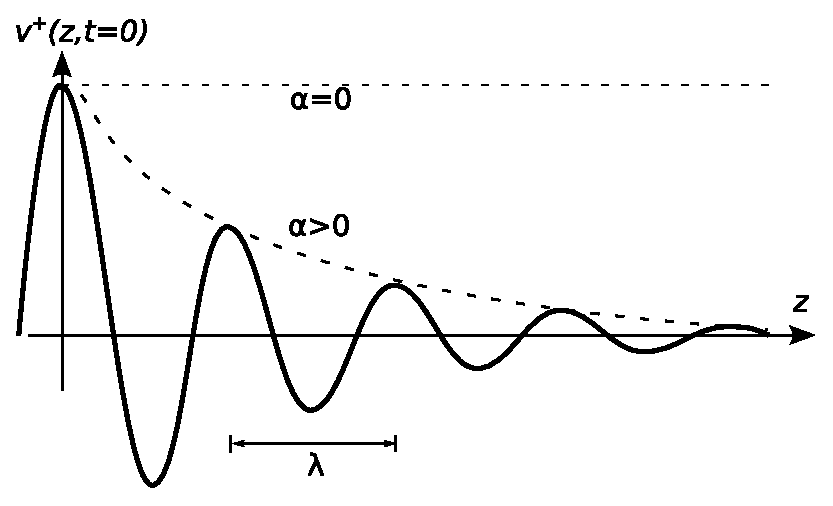
\includegraphics[width=\columnwidth]{modules/m0080_fVwave.eps}
}}{A graph depicting a wave traveling across the z-axis with 5 peaks. The first wave peak intersects the y-axis and is labeled v superscript + (z,t=0). At the top of the first peak, a dotted line extends perpendicularly to the right labeled alpha=0. Also at the top of the first peak, a dotted line curves downward with decreasing slope and is labeled alpha>0. As the wave oscillates to the right along the z-axis, the peaks decrease in height. Between the second and third peaks, a line underneath the graph shows the wavelength lambda.}
\end{center} 
\caption{\label{m0080_fVwave}The potential $v^+(z,t)$ of the wave traveling in the $+z$ direction at $t=0$ for $\psi=0$.}
\end{figure}

Also we recognize:
%ORB HIGHLIGHT
\begin{mdframed}[backgroundcolor=yellow!20,nobreak=true] 
$\alpha\triangleq\mbox{Re}\left\{\gamma\right\}$ (1/m) is the \emph{attenuation constant}, 
\index{propagation constant!attenuation}
\index{attenuation constant|see {propagation constant}}
which is the rate at which magnitude diminishes as a function of distance. 
\end{mdframed}

Sometimes the units of $\alpha$ are indicated as ``Np/m'' (``nepers'' per meter), where the term ``neper'' 
\index{neper}
is used to indicate the units of the otherwise unitless real-valued exponent of the constant $e$.

Note that $\alpha=0$ for a wave that does not diminish in magnitude with increasing distance, in which case the transmission line is said to be \emph{lossless}.
\index{transmission line!lossless}
If $\alpha>0$ then the line is said to be \emph{lossy} (or possibly ``low loss'' if the loss can be neglected), 
\index{transmission line!low loss}
and in this case the rate at which the magnitude decreases with distance increases with $\alpha$.  

Next let us consider the speed of the wave.
To answer this question, we need to be a bit more specific about what we mean by ``speed.''
At the moment, we mean phase velocity; 
that is, the speed at which a point of constant phase seems to move through space.
In other words, what distance $\Delta z$ does a point of constant phase traverse in time $\Delta t$?
To answer this question, we first note that the phase of $v^+(z,t)$ can be written generally as 
%
\begin{equation}
\omega t - \beta z + \phi
\nonumber
\end{equation}
%
where $\phi$ is some constant.  
Similarly, the phase at some time $\Delta t$ later and some point $\Delta z$ further along can be written as 
%
\begin{equation}
\omega \left( t +\Delta t \right) - \beta \left( z +\Delta z \right) + \phi
\nonumber
\end{equation}
The phase velocity $v_p$ is $\Delta z/\Delta t$ when these two phases are equal; i.e., when
%
\begin{equation}
\omega t - \beta z + \phi = \omega \left( t +\Delta t \right) - \beta \left( z +\Delta z \right) + \phi
\nonumber
\end{equation}   
%
Solving for $v_p=\Delta z/\Delta t$, we obtain:
%
\begin{equation}
\boxed{ v_p = \frac{\omega}{\beta} }
\end{equation}
%
Having previously noted that $\beta = 2\pi/\lambda$, the above expression also yields the expected result
%
\begin{equation}
\boxed{
v_p = \lambda f
}
\end{equation}
%
%ORB HIGHLIGHT
\begin{mdframed}[backgroundcolor=yellow!20,nobreak=true] 
The phase velocity 
\index{phase velocity}
$v_p = \omega/\beta = \lambda f$ is the speed at which a point of constant phase travels along the line.
\end{mdframed}

Returning now to consider the current associated with the wave traveling in the $+z$ direction:
%
\begin{equation}
\widetilde{I}^+(z) = I_0^+ e^{-\gamma z} 
\end{equation}
%
We can rewrite this expression in terms of the characteristic impedance 
\index{characteristic impedance}
$Z_0$, as follows:
%
\begin{equation}
\widetilde{I}^+(z) = \frac{V_0^+}{Z_0} e^{-\gamma z}
\end{equation}
%
Similarly, we find that the current $\widetilde{I}^-(z)$ associated with $\widetilde{V}^-(z)$ for the wave traveling in the $-z$ direction is
%
\begin{equation}
\widetilde{I}^-(z) = \frac{-V_0^-}{Z_0} e^{-\gamma z}
\end{equation}
%
The negative sign appearing in the above expression emerges as a result of the sign conventions used for potential and current in the derivation of the telegrapher's equations (Section~\ref{m0079_Telegraphers_Equations}).
The physical significance of this change of sign is that wherever the potential of the wave traveling in the $-z$ direction is positive, then the current at the same point is flowing in the $-z$ direction. 

It is frequently necessary to consider the possibility that waves travel in both directions simultaneously. 
A very important case where this arises is when there is reflection from a discontinuity of some kind; e.g., from a termination which is not perfectly impedance-matched.
In this case, the total potential $\widetilde{V}(z)$ and total current $\widetilde{I}(z)$ can be expressed as the general solution to the wave equation; i.e., as the sum of the ``incident'' ($+z$-traveling) wave and the reflected ($-z$-traveling) waves:
%
\begin{equation}
\widetilde{V}(z) = \widetilde{V}^+(z) + \widetilde{V}^-(z)
\end{equation}
%
\begin{equation}
\widetilde{I}(z) = \widetilde{I}^+(z) + \widetilde{I}^-(z)
\end{equation}
%
The existence of waves propagating simultaneously in both directions gives rise to a phenomenon known as a \emph{standing wave}. 
\index{waves!standing|see{standing wave}}
\index{standing wave}
Standing waves and the calculation of the coefficients $V_0^{-}$ and $I_0^{-}$ due to reflection are addressed in Sections~\ref{m0086_Standing_Waves} and \ref{m0084_Voltage_Reflection_Coefficient} respectively.


      \vfill\break
    \section{Lossless and Low-Loss Transmission Lines}
{\color{blue}\tiny[m0083]}      % This is text associated with the open textbook "Open Electromagnetics"
% See immediately below for author, date
% This work is licensed under the Creative Commons Attribution-ShareAlike 4.0 International License. (CC BY-SA 4.0) 
% To view a copy of the license, visit http://creativecommons.org/licenses/by-sa/4.0/

%ORB TITLE Lossless and Low-Loss Transmission Lines
%ORB AUTHOR 0        # S.W. Ellingson, Virginia Tech (ellingson@vt.edu)
%ORB DATE 20180802   # yyyymmdd
%ORB ABSTRACT Simpler forms of alpha, beta, Z0 etc when line is lossless 

\label{m0083_Lossless_Transmission_Lines} % <-- Must match name of this file and module directory name.  Don't mess with this!

Quite often the loss in a transmission line is small enough that it may be neglected.  
In this case, several aspects of transmission line theory may be simplified.  
In this section, we present these simplifications.

First, recall that ``loss'' refers to the reduction of magnitude as a wave propagates through space. 
In the lumped-element equivalent circuit model 
\index{transmission line!lumped-element model}
(Section~\ref{m0029_Lumped-Element_Model}), the parameters $R'$ and $G'$ of the represent physical mechanisms associated with loss.
Specifically, $R'$ represents the resistance of conductors, whereas $G'$ represents the undesirable current induced between conductors through the spacing material.
Also recall that the propagation constant $\gamma$ is, in general, given by
%
\begin{equation}
\gamma \triangleq \sqrt{\left(R'+j\omega L'\right)\left(G'+j\omega C'\right)}
\end{equation} 

With this in mind, we now define ``low loss''
\index{transmission line!low loss}
as meeting the conditions:
%
\begin{equation}
R'\ll\omega L'
\label{m0083_eLLR}
\end{equation}
%
\begin{equation}
G'\ll\omega C'
\label{m0083_eLLG}
\end{equation}
%
When these conditions are met, the propagation constant simplifies as follows:
%
\begin{flalign}
\gamma &\approx \sqrt{\left(j\omega L'\right)\left(j\omega C'\right)} \nonumber \\
       &= \sqrt{-\omega^2 L'C'} \nonumber \\
       &= j\omega\sqrt{L'C'} 
\end{flalign} 
%
and subsequently
%
\begin{flalign}
\alpha \triangleq \mbox{Re}\left\{\gamma\right\} & \approx 0                     & \mbox{(low-loss approx.)} \\
\beta  \triangleq \mbox{Im}\left\{\gamma\right\} & \approx \omega\sqrt{L'C'}     & \mbox{(low-loss approx.)} \\
v_p    = \omega/\beta                            & \approx \frac{1}{\sqrt{L'C'}} & \mbox{(low-loss approx.)}
\end{flalign}
%
Similarly:
\begin{equation}
Z_0 = \sqrt{\frac{R' + j\omega L'}{G' + j\omega C'}} \approx \sqrt{\frac{L'}{C'}} ~~~ \mbox{(low-loss approx.)}
\end{equation} 

Of course if the line is strictly lossless (i.e., $R'=G'=0$) then these are not approximations, but rather the exact expressions.

In practice, these approximations are quite commonly used, since practical transmission lines typically meet the conditions expressed in Inequalities~\ref{m0083_eLLR} and \ref{m0083_eLLG} and the resulting expressions are much simpler.  We further observe that $Z_0$ and $v_p$ are approximately independent of frequency when these conditions hold.

However, also note that ``low loss'' does not mean ``no loss,'' and it is common to apply these expressions even when $R'$ and/or $G'$ is large enough to yield significant loss.  For example, a coaxial cable used to connect an antenna on a tower to a radio near the ground typically has loss that is important to consider in the analysis and design process, but nevertheless satisfies Equations~\ref{m0083_eLLR} and \ref{m0083_eLLG}.  In this case, the low-loss expression for $\beta$ is used, but $\alpha$ might not be approximated as zero.
 




      \vfill\break
    \section{Coaxial Line}
{\color{blue}\tiny[m0143]}      % This is text associated with the open textbook "Open Electromagnetics"
% See immediately below for author, date
% This work is licensed under the Creative Commons Attribution-ShareAlike 4.0 International License. (CC BY-SA 4.0) 
% To view a copy of the license, visit http://creativecommons.org/licenses/by-sa/4.0/

%ORB TITLE Coaxial Line
%ORB AUTHOR 0        # S.W. Ellingson, Virginia Tech (ellingson@vt.edu)
%ORB DATE 20180802   # yyyymmdd
%ORB ABSTRACT

\label{m0143_Coaxial_Line} % <-- Must match name of this file and module directory name.  Don't mess with this!
\index{transmission line!coaxial|(}

Coaxial transmission lines consists of metallic inner and outer conductors separated by a spacer material as shown in Figure~\ref{m0143_fCoaxCrossSection}. 
The spacer material is typically a low-loss dielectric 
\index{dielectric (material)}
material having permeability approximately equal to that of free space ($\mu\approx\mu_0$) and permittivity $\epsilon_s$ that may range from very near $\epsilon_0$ (e.g., air-filled line) to 2--3 times $\epsilon_0$. 
The outer conductor is alternatively referred to as the ``shield,'' 
\index{shield}
since it typically provides a high degree of isolation from nearby objects and electromagnetic fields.
Coaxial line is single-ended\footnote{The references in ``Additional Reading'' at the end of this section may be helpful if you are not familiar with this concept.} in the sense that the conductor geometry is asymmetric and the shield is normally attached to ground at both ends.
These characteristics make coaxial line attractive for connecting single-ended circuits in widely-separated locations and for connecting antennas to receivers and transmitters.
%
\begin{figure}
\begin{center}
\pdftooltip{{  % note double braces
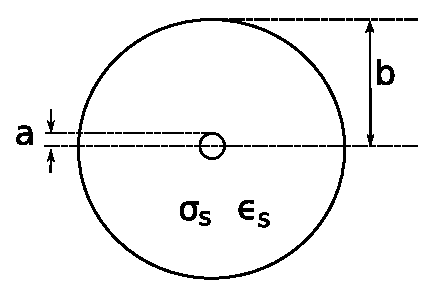
\includegraphics[width=2in]{modules/m0143_fCoaxCrossSection.eps}
}}{A small circle is concentric with a much larger circle. The radius of the small circle is called "a". The radius of the larger circle is called "b". The design parameters of epsilon sub r and sigma sub s are shown in the area between the circles.}
\end{center}
%\vspace{2.5in}
\caption{\label{m0143_fCoaxCrossSection}Cross-section of a coaxial transmission line, indicating design parameters.}
\end{figure} 

Coaxial lines exhibit TEM 
\index{transmission line!transverse electromagnetic (TEM)}
field structure as shown in Figure~\ref{m0143_fCoaxFieldStructure}.
%
\begin{figure}
\begin{center}
\pdftooltip{{  % note double braces
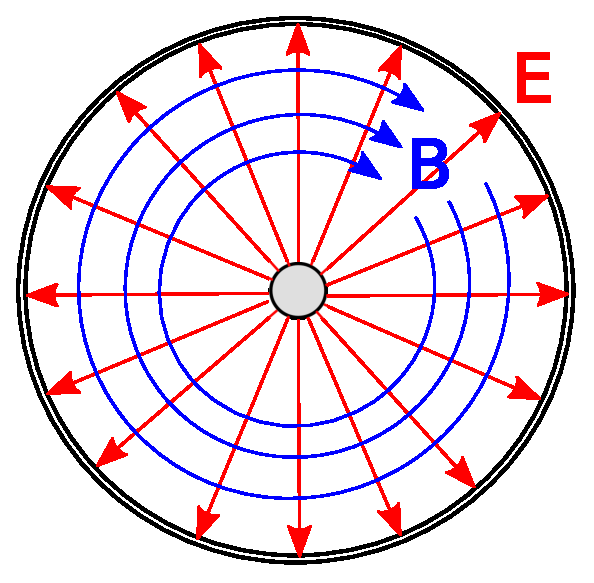
\includegraphics[width=1.5in]{modules/m0143_fCoaxFieldStructure.eps}
}}{A cross-sectional view of a coaxial transmission line. The inner conductor is represented by a gray-filled circle.  The electric field, "E", is represented by red arrows pointing outward from the inner conductor to the outer conductor which is represented by a larger concentric circle. The magnetic field, "B", is represented by concentric, circular blue arrows between the insulating jacket and the inner conductor. The arrows indicate a clockwise direction.}
\end{center} 
\caption{\label{m0143_fCoaxFieldStructure}Structure of the electric and magnetic fields within coaxial line.  In this case, the wave is propagating away from the viewer.}
\end{figure}
 
Expressions for the equivalent circuit parameters $C'$ and $L'$ for coaxial lines can be obtained from basic electromagnetic theory.
It is shown in Section~\ref{m0113_Capacitance_of_Coaxial_Line} that the capacitance per unit length is
%
\begin{equation}
C' = \frac{2\pi\epsilon_s}{\ln\left(b/a\right)}
\label{m0143_eCp}
\end{equation}
%
where $a$ and $b$ are the radii of the inner and outer conductors, respectively.
Using analysis shown in Section~\ref{m0125_Inductance_of_a_Coaxial_Transmission_Line}, the inductance per unit length is
%
\begin{equation}
L' = \frac{\mu_0}{2\pi}\ln\left(\frac{b}{a}\right)
\label{m0143_eLp}
\end{equation}
%
The loss conductance $G'$ depends on the conductance $\sigma_s$ of the spacer material, and is given by 
%
\begin{equation}
G' = \frac{2\pi\sigma_s}{\ln\left(b/a\right)}
\end{equation}
%
This expression is derived in Section~\ref{m0105_Conductance_DC}.

The resistance per unit length, $R'$, is relatively difficult to quantify.
One obstacle is that the inner and outer conductors typically consist of different materials or compositions of materials.
The inner conductor is not necessarily a single homogeneous material; instead, the inner conductor may consist of a variety of materials selected by trading-off between conductivity, strength, weight, and cost.
Similarly, the outer conductor is not necessarily homogeneous; for a variety of reasons, the outer conductor may instead be a metal mesh, a braid, or a composite of materials.
Another complicating factor is that the resistance of the conductor varies significantly with frequency, whereas $C'$, $L'$, and $G'$ exhibit relatively little variation from their electro- and magnetostatic values.
These factors make it difficult to devise a single expression for $R'$ that is both as simple as those shown above for the other parameters and generally applicable.
Fortunately, it turns out that the low-loss 
\index{transmission line!low loss}
conditions $R'\ll\omega L'$ and $G'\ll\omega C'$ are often applicable,\footnote{See Section~\ref{m0083_Lossless_Transmission_Lines} for a reminder about this concept.} so that $R'$ and $G'$ are important only if it is necessary to compute loss. 

Since the low-loss conditions are often met, a convenient expression for the characteristic impedance 
\index{characteristic impedance!coaxial cable}
is obtained from Equations~\ref{m0143_eCp} and \ref{m0143_eLp} for $L'$ and $C'$ respectively:
%
\begin{flalign}
Z_0 & \approx \sqrt{\frac{L'}{C'}} ~~~\mbox{(low-loss)} \nonumber \\
    & = \frac{1}{2\pi}\sqrt{\frac{\mu_0}{\epsilon_s}}\ln{\frac{b}{a}} 
\end{flalign}
%
The spacer permittivity can be expressed as $\epsilon_s=\epsilon_r\epsilon_0$ where $\epsilon_r$ is the relative permittivity of the spacer material.
Since $\sqrt{\mu_0/\epsilon_0}$ is a constant, the above expression is commonly written
%
\begin{equation}
Z_0 \approx \frac{60~\Omega}{\sqrt{\epsilon_r}} \ln{\frac{b}{a}} ~~~\mbox{(low-loss)}
\end{equation}
%
Thus, it is possible to express $Z_0$ directly in terms of parameters describing the geometry ($a$ and $b$) and material ($\epsilon_r$) used in the line, without the need to first compute the values of components in the lumped-element equivalent circuit model.

Similarly, the low-loss approximation makes it possible to express the phase velocity $\nu_p$ directly in terms the spacer permittivity:
\index{phase velocity!coaxial cable}
%
\begin{flalign}
\nu_p & \approx \frac{1}{\sqrt{L'C'}} ~~~\mbox{(low-loss)} \nonumber \\
      & = \frac{c}{\sqrt{\epsilon_r}}
\end{flalign}
%
since $c\triangleq 1/\sqrt{\mu_0\epsilon_0}$.
In other words, the phase velocity in a low-loss coaxial line is approximately equal to the speed of electromagnetic propagation in free space, divided by the square root of the relative permittivity of the spacer material. 
Therefore, the phase velocity in an air-filled coaxial line is approximately equal to speed of propagation in free space, but is reduced in a coaxial line using a dielectric spacer.

%ORB EXAMPLE
~\\ \begin{example} 
\begin{mdframed}[backgroundcolor=brown!20,linecolor=brown!20]\raggedright 
RG-59 
\index{RG-59}
Coaxial Cable. 
\\~\\
RG-59 is a very common type of coaxial line.
Figure~\ref{m0143_fRG-59} shows a section of RG-59 cut away so as to reveal its structure.
The radii are $a\cong 0.292$~mm and $b\approx 1.855$~mm (mean), yielding $L'\approx 370$~nH/m.
The spacer material is polyethylene having $\epsilon_r\cong 2.25$, yielding $C'\approx 67.7$~pF/m.
The conductivity of polyethylene is $\sigma_s\cong 5.9 \times 10^{-5}$~S/m, yielding $G'\approx 200~\mu$S/m.
Typical resistance per unit length $R'$ is on the order of $0.1~\Omega$/m near DC, increasing approximately in proportion to the square root of frequency. 

From the above values, we find that RG-59 satisfies the low-loss criteria 
$R'\ll\omega L'$ for $f\gg 43$~kHz and 
$G'\ll\omega C'$ for $f\gg 470$~kHz.
Under these conditions, we find $Z_0 \approx \sqrt{L'/C'} \cong 74~\Omega$.    
Thus, the ratio of the potential to the current in a wave traveling in a single direction on RG-59 is about $74~\Omega$.

The phase velocity of RG-59 is found to be $v_p \approx 1/\sqrt{L'C'} \cong 2 \times 10^8$~m/s, which is about 67\% of $c$.  In other words, a signal that takes 1~ns to traverse a distance $l$ in free space requires about 1.5~ns to traverse a length-$l$ section of RG-59. 
Since $v_p = \lambda f$, a wavelength in RG-59 is 67\% of a wavelength in free space.

Using the expression 
%
\begin{equation}
\gamma = \sqrt{\left(R'+j\omega L'\right)\left(G'+j\omega C'\right)}
\end{equation} 
%
with $R'=0.1~\Omega$/m, and then taking the real part to obtain $\alpha$, we find $\alpha\sim 0.01$~m$^{-1}$.  So, for example, the magnitude of the potential or current is decreased by about 50\% by traveling a distance of about 70~m. 
In other words, $e^{-\alpha l} = 0.5$ for $l \sim 70$~m at relatively low frequencies, and increases with increasing frequency.    

\end{mdframed} 

\begin{figure}
\begin{center}
\pdftooltip{{  % note double braces
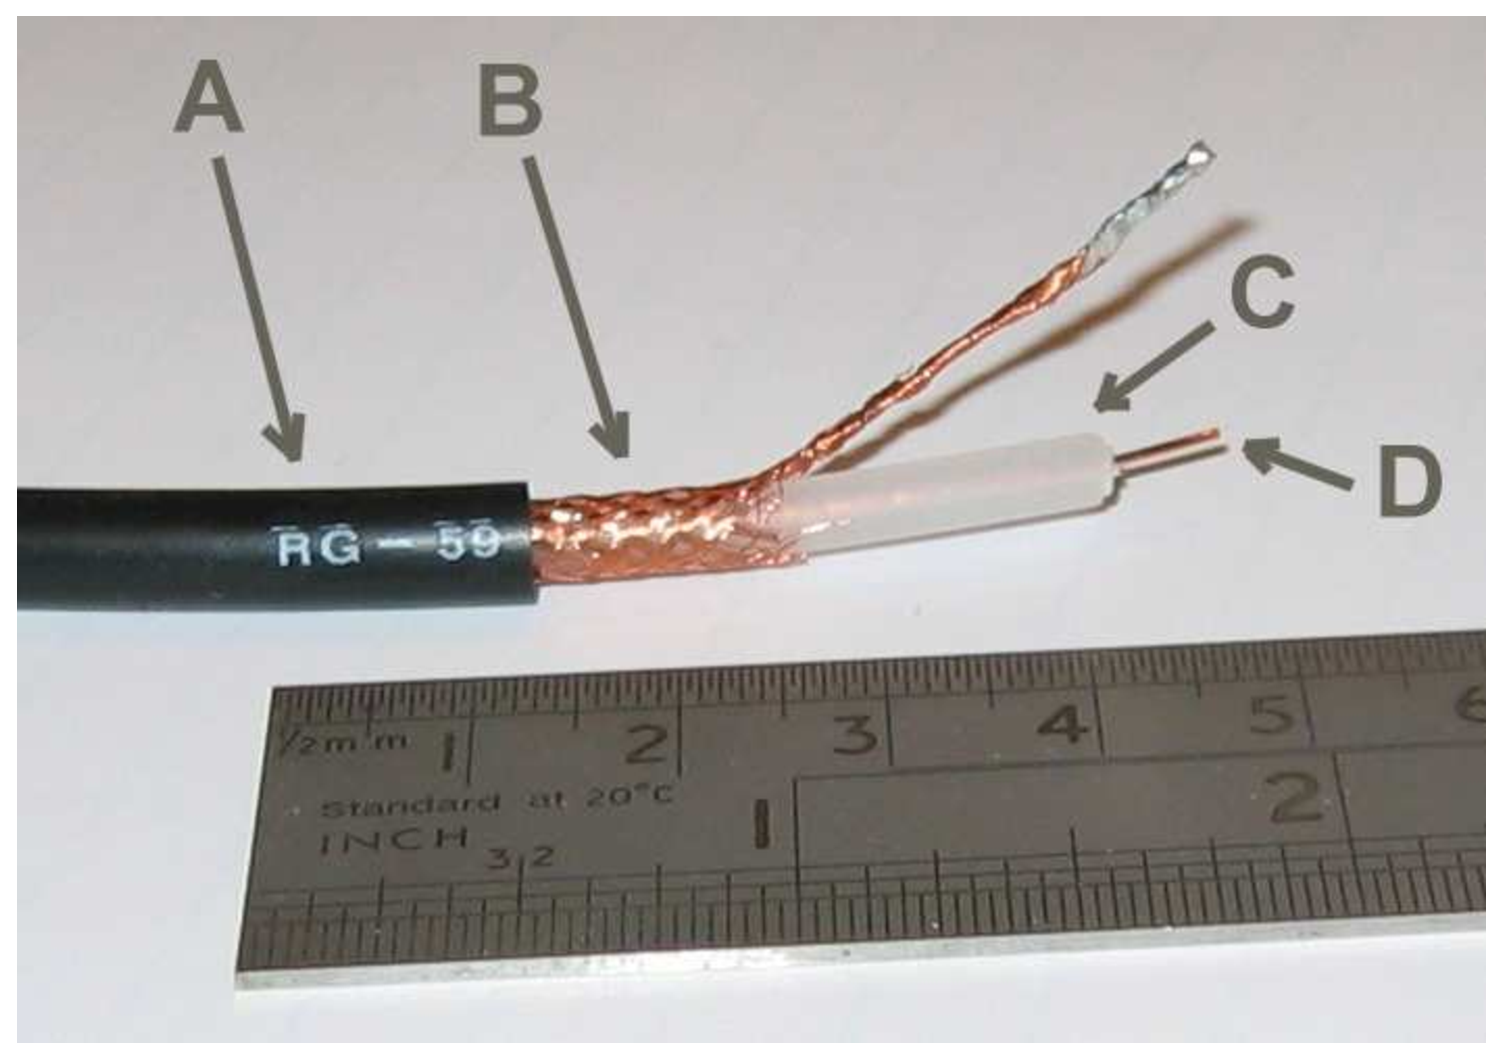
\includegraphics[width=2.5in]{modules/m0143_fRG-59.eps}
% https://en.wikipedia.org/wiki/File:RG-59.jpg
}}{A photo of a dissected coaxial line. A ruler is sitting next to the coaxial line for reference. About 3 cm of the line is missing the insulating jacket. The braided outer conductor is removed over a 1.5 cm section of the dielectric spacer. A 0.5 cm section of dielectric spacer is removed, exposing the inner conductor.}
\end{center} 
\centerline{\scriptsize 
\copyright~\hyperref[m0143_fRG-59_Credit]{Arj} 
\href{https://creativecommons.org/licenses/by-sa/3.0/}{CC BY~SA 3.0} 
} 
\caption{
\label{m0143_fRG-59}
RG-59 coaxial line. A: Insulating jacket. B: Braided outer conductor. C: Dielectric spacer. D: Inner conductor. 
}
\end{figure}

\end{example}

%%%%%%%%%%%%%%%%%%%%%%%%%%%%%%%%

{\bf Additional Reading:}
\begin{itemize}
\item ``\href{https://en.wikipedia.org/wiki/Coaxial_cable}{Coaxial cable}'' on Wikipedia. \emph{Includes descriptions and design parameters for a variety of commonly-encountered coaxial cables.}
\item ``\href{https://en.wikipedia.org/wiki/Single-ended_signaling}{Single-ended signaling}'' on Wikipedia.
\item Sec.~8.7 (``Differential Circuits'') in S.W.~Ellingson, \emph{Radio Systems Engineering}, Cambridge Univ.\ Press, 2016. 
\end{itemize}

\index{transmission line!coaxial|)}

      \vfill\break
    \section{Microstrip Line}
{\color{blue}\tiny[m0082]}      % This is text associated with the open textbook "Open Electromagnetics"
% See immediately below for author, date
% This work is licensed under the Creative Commons Attribution-ShareAlike 4.0 International License. (CC BY-SA 4.0) 
% To view a copy of the license, visit http://creativecommons.org/licenses/by-sa/4.0/

%ORB TITLE Microstrip Line
%ORB AUTHOR 0        # S.W. Ellingson, Virginia Tech (ellingson@vt.edu)
%ORB DATE 20180802   # yyyymmdd
%ORB ABSTRACT Basics of microstrip lines in terms of elementary transmission line theory 

\label{m0082_Microstrip_Line} % <-- Must match name of this file and module directory name.  Don't mess with this!
\index{microstrip|(}
\index{transmission line!microstrip|see{microstrip}}

A microstrip transmission line consists of a narrow metallic trace separated from a metallic ground plane by a slab of dielectric material, as shown in Figure~\ref{m0082_fMicrostripCrossSection}. 
This is a natural way to implement a transmission line on a printed circuit board,
\index{printed circuit board (PCB)}
and so accounts for an important and expansive range of applications.
The reader should be aware that microstrip is distinct from \emph{stripline},
\index{stripline}
\index{transmission line!stripline}
which is a very different type of transmission line; see ``Additional Reading'' at the end of this section for disambiguation of these terms.
%
\begin{figure}
\begin{center}
\pdftooltip{{  % note double braces
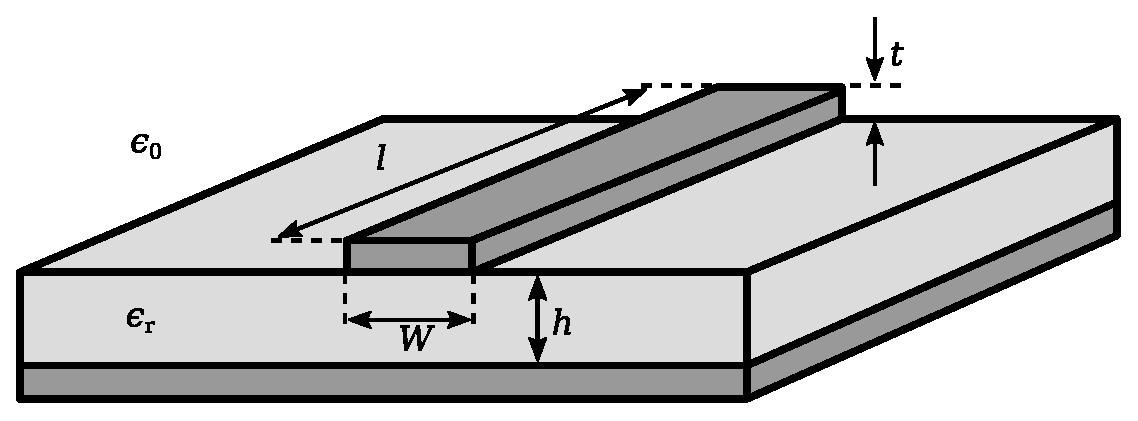
\includegraphics[width=\columnwidth]{modules/m0082_fMicrostripCrossSection.eps}
% https://commons.wikimedia.org/wiki/File:Microstrip_scheme.svg
}}{A diagram of a microstrip transmission line. Certain dimensions are labeled: Length of the metal trace (l), width of the metal trace (W), thickness of the metal trace (t), and height of the dielectric slab (h). Epsilon sub r is labeled on the dielectric and epsilon sub 0 is labeled on the space next to the microstrip transmission line.}
\end{center} 
\centerline{\scriptsize 
\copyright~\hyperref[m0082_fMicrostripCrossSection_Credit]{7head7metal7}  
\href{https://creativecommons.org/licenses/by-sa/3.0/}{CC BY~SA 3.0} 
(modified)
} 
\caption{
\label{m0082_fMicrostripCrossSection}
Microstrip transmission line structure and design parameters.
}
\end{figure}

A microstrip line is single-ended\footnote{The reference in ``Additional Reading'' at the end of this section may be helpful if you are not familiar with this concept.} in the sense that the conductor geometry is asymmetric and the one conductor -- namely, the ground plane -- also normally serves as ground for the source and load.

The spacer material is typically a low-loss dielectric 
\index{dielectric (material)}
material having permeability approximately equal to that of free space ($\mu \approx \mu_0$) and relative permittivity $\epsilon_r$ in the range 2 to about 10 or so.

A microstrip line nominally exhibits TEM 
\index{transmission line!transverse electromagnetic (TEM)}
field structure.
This structure is shown in Figure~\ref{m0082_fMicrostripFieldStructure}.
Note that electric and magnetic fields exist both in the dielectric and in the space above the dielectric, which is typically (but not always) air. 
This complex field structure makes it difficult to describe microstrip line concisely in terms of the equivalent circuit parameters of the lumped-element model.  
Instead, expressions for $Z_0$ directly in terms of $h/W$ and $\epsilon_r$ are typically used instead.  
A variety of these expressions are in common use, representing different approximations and simplifications.  
A widely-accepted and broadly-applicable expression is:\footnote{This is from Wheeler 1977, cited in ``Additional Reading'' at the end of this section.}
%
\begin{equation}
\begin{split}
Z_0 & \approx \frac{42.4~\Omega}{\sqrt{\epsilon_r+1}} ~\times \\
    &
\ln\left[
    1 +
    \frac{4h}{W'}
    \left( \Phi + \sqrt{ \Phi^2 + \frac{1+1/\epsilon_r}{2}\pi^2 } \right)
   \right]
\end{split}
\label{m0082_eWheeler10}
\end{equation}
% 
where
%
\begin{equation}
\Phi \triangleq \frac{ 14 + 8/\epsilon_r }{ 11 } \left( \frac{4h}{W'} \right)
\end{equation}
%
and $W'$ is $W$ adjusted to account for the thickness $t$ of the microstrip line.  Typically $t\ll W$ and $t \ll h$, for which $W'\approx W$.  
Simpler approximations for $Z_0$ are also commonly employed in the design and analysis of microstrip lines. 
These expressions are limited in the range of $h/W$ for which they are valid, and can usually be shown to be special cases or approximations of Equation~\ref{m0082_eWheeler10}.
Nevertheless, they are sometimes useful for quick ``back of the envelope'' calculations.
%
\begin{figure}
\begin{center}
\pdftooltip{{  % note double braces
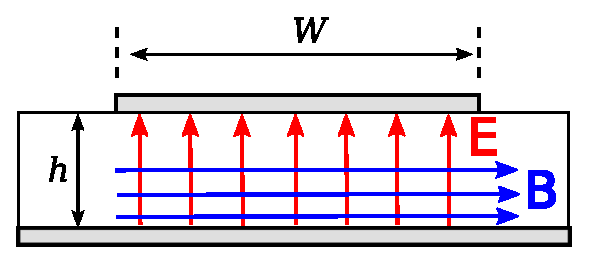
\includegraphics[width=2.5in]{modules/m0082_fMicrostripFieldStructure.eps}
}}{A cross-sectional view of the microstrip transition line. The electric field, "E", is represented by a row of red parallel arrows pointing vertically from the ground plane to the metallic trace.The magnetic field, "B", is represented by parallel blue arrows perpendicular to the electric field arrows, pointing to the right.}
\end{center} 
\caption{\label{m0082_fMicrostripFieldStructure}Structure of the electric and magnetic fields within microstrip line. (The fields \emph{outside} the line are possibly significant, complicated, and not shown.)  In this case, the wave is propagating away from the viewer.}
\end{figure}

Accurate expressions for wavelength $\lambda$, phase propagation constant $\beta$, and phase velocity $v_p$ are similarly difficult to obtain for waves in microstrip line.
An approximate technique employs a result from the theory of uniform plane waves in unbounded media (Equation~\ref{m0036_eBetaDef} from Section~\ref{m0036_Wave_Equations_SourceFree_Lossless}):
%
\begin{equation}
\beta = \omega\sqrt{\mu\epsilon}
\end{equation}
%
It turns out that the electromagnetic field structure in the space between the conductors is well-approximated as that of a uniform plane wave in unbounded media having the same permeability $\mu_0$ but a different relative permittivity, which we shall assign the symbol $\epsilon_{r,eff}$ (for ``\emph{effective} relative permittivity''). 
\index{permittivity!effective}
Then
%
\begin{flalign}
\beta &\approx \omega\sqrt{\mu_0~\epsilon_{r,eff}~\epsilon_0} ~~~\mbox{(low-loss microstrip)} \nonumber \\
      &=\beta_0 \sqrt{\epsilon_{r,eff}}
\end{flalign}
%
In other words, the phase propagation constant in a microstrip line can be approximated as the free-space phase propagation $\beta_0\triangleq\omega\sqrt{\mu_0\epsilon_0}$ times a correction factor $\sqrt{\epsilon_{r,eff}}$. 
Then $\epsilon_{r,eff}$ may be crudely approximated as follows:
%
\begin{equation}
\epsilon_{r,eff} \approx \frac{\epsilon_r+1}{2}
\end{equation}
%
i.e., $\epsilon_{r,eff}$ is roughly the average of the relative permittivity of the dielectric slab and the relative permittivity of free space.  
The assumption employed here is that $\epsilon_{r,eff}$ is approximately the average of these values because some fraction of the power in the guided wave is in the dielectric, and the rest is above the dielectric.
Various approximations are available to improve on this approximation; however, in practice variations in the value of $\epsilon_r$ for the dielectric due to manufacturing processes typically make a more precise estimate irrelevant.

Using this concept, we obtain
%
\begin{equation}
\lambda = \frac{2\pi}{\beta} = \frac{2\pi}{\beta_0\sqrt{\epsilon_{r,eff}}} = \frac{\lambda_0}{\sqrt{\epsilon_{r,eff}}}
\end{equation}
%
where $\lambda_0$ is the free-space wavelength
\index{wavelength!in microstrip}
$c/f$.
Similarly the phase velocity 
\index{phase velocity!in microstrip}
$v_p$, can be estimated using the relationship
%
\begin{equation}
v_p = \frac{\omega}{\beta} = \frac{c}{\sqrt{\epsilon_{r,eff}}}
\end{equation}
%
i.e., the phase velocity in microstrip is slower than $c$ by a factor of $\sqrt{\epsilon_{r,eff}}$.

%ORB EXAMPLE
~\\ \begin{example} 
\begin{mdframed}[backgroundcolor=brown!20,linecolor=brown!20]\raggedright
$50~\Omega$ Microstrip in FR4 
\index{FR4}
Printed Circuit Boards.
\index{printed circuit board (PCB)}
\\~\\
FR4 is a low-loss fiberglass epoxy dielectric that is commonly used to make printed circuit boards (see ``Additional Reading'' at the end of this section).
FR4 circuit board material is commonly sold in a slab having thickness $h\cong 1.575$~mm 
%(62~mils) 
with $\epsilon_r\cong 4.5$.  
Let us consider how we might implement a microstrip line having $Z_0=50~\Omega$ using this material.
Since $h$ and $\epsilon_r$ are fixed, the only parameter remaining to set $Z_0$ is $W$.
A bit of experimentation with Equation~\ref{m0082_eWheeler10} reveals that $h/W\approx 1/2$ yields $Z_0\approx 50~\Omega$ for $\epsilon_r=4.5$.  
Thus, $W$ should be about 3.15~mm.
The effective relative permittivity is 
%
\begin{equation}
\epsilon_{r,eff}\approx(4.5+1)/2 = 2.75
\nonumber
\end{equation}
%
so the phase velocity for the wave guided by this line is about $c/\sqrt{2.75}$; i.e., 60\% of $c$.
Similarly, the wavelength of this wave is about 60\% of the free space wavelength.
\end{mdframed}\end{example}

%------------------------------------

{\bf Additional Reading:}
\begin{itemize}
\item ``\href{https://en.wikipedia.org/wiki/Microstrip}{Microstrip}'' on Wikipedia.
\item ``\href{https://en.wikipedia.org/wiki/Printed_circuit_board}{Printed circuit board}'' on Wikipedia.
\item ``\href{https://en.wikipedia.org/wiki/Stripline}{Stripline}'' on Wikipedia.
\item ``\href{https://en.wikipedia.org/wiki/Single-ended_signaling}{Single-ended signaling}'' on Wikipedia.
\item Sec.~8.7 (``Differential Circuits'') in S.W.~Ellingson, \emph{Radio Systems Engineering}, Cambridge Univ.\ Press, 2016. 
\item H.A.\ Wheeler, ``Transmission Line Properties of a Strip on a Dielectric Sheet on a Plane,'' {\it IEEE Trans.\ Microwave Theory \& Techniques}, Vol.~25, No.~8, Aug~1977, pp.~631--47. % http://dx.doi.org/10.1109/TMTT.1977.1129179.
\item ``\href{https://en.wikipedia.org/wiki/FR-4}{FR-4}'' on Wikipedia.
\end{itemize}
 
\index{microstrip|)}


      \vfill\break
    \section{Voltage Reflection Coefficient}
{\color{blue}\tiny[m0084]}      % This is text associated with the open textbook "Open Electromagnetics"
% See immediately below for author, date
% This work is licensed under the Creative Commons Attribution-ShareAlike 4.0 International License. (CC BY-SA 4.0) 
% To view a copy of the license, visit http://creativecommons.org/licenses/by-sa/4.0/

%ORB TITLE Voltage Reflection Coefficient
%ORB AUTHOR 0        # S.W. Ellingson, Virginia Tech (ellingson@vt.edu)
%ORB DATE 20180802   # yyyymmdd
%ORB ABSTRACT Voltage reflection coefficient for a lossless transmission line

\label{m0084_Voltage_Reflection_Coefficient} % <-- Must match name of this file and module directory name.  Don't mess with this!
\index{reflection coefficient|(}
\index{voltage reflection coefficient|see{reflection coefficient}}

We now consider the scenario shown in Figure~\ref{m0084_fWaveIncidentOnZL}. 
Here a wave arriving from the left along a lossless transmission line having characteristic impedance $Z_0$ arrives at a termination located at $z=0$.
The impedance looking into the termination is $Z_L$, which may be real-, imaginary-, or complex-valued.
The questions are: Under what circumstances is a reflection -- i.e., a leftward traveling wave -- expected, and what precisely is that wave?
%
\begin{figure}[b!]
\begin{center}
\pdftooltip{{  % note double braces
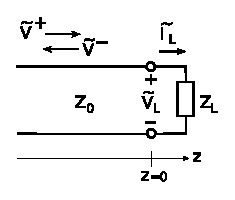
\includegraphics[width=2in]{modules/m0084_fWaveIncidentOnZL.eps}
}}{A lossless transmission line with a wave arriving from the left and with reflected wave traveling to the left. The transmission line is open on the left side with a load on the right side. The current is shown going through the load clockwise.}
\end{center} 
\caption{\label{m0084_fWaveIncidentOnZL}A wave arriving from the left incident on a termination located at $z=0$.}
\end{figure}

The potential and current of the incident wave are related by the constant value of $Z_0$.
Similarly, the potential and current of the reflected wave are related by $Z_0$. 
Therefore, it suffices to consider \emph{either} potential or current.  
Choosing potential, we may express the incident wave as 
%
\begin{equation}
\widetilde{V}^+(z) = V_0^+ e^{-j\beta z}
\end{equation} 
%
where $V_0^+$ is determined by the source of the wave, and so is effectively a ``given.''
Any reflected wave must have the form
%
\begin{equation}
\widetilde{V}^-(z) = V_0^- e^{+j\beta z}
\end{equation} 
%
Therefore, the problem is solved by determining the value of $V_0^-$ given $V_0^+$, $Z_0$, and $Z_L$.

Considering the situation at $z=0$, note that by definition we have
%
\begin{equation}
Z_L \triangleq \frac{\widetilde{V}_L}{\widetilde{I}_L}
\label{m0084_eZL}
\end{equation}
%
where $\widetilde{V}_L$ and $\widetilde{I}_L$ are the potential across and current through the termination, respectively.
Also, the potential and current on either side of the $z=0$ interface must be equal. Thus,
%
\begin{flalign}
\widetilde{V}^+(0) + \widetilde{V}^-(0) & = \widetilde{V}_L \label{m0084_eV1} \\
\widetilde{I}^+(0) + \widetilde{I}^-(0) & = \widetilde{I}_L \label{m0084_eI1}
\end{flalign}
%
where $\widetilde{I}^+(z)$ and $\widetilde{I}^-(z)$ are the currents associated with $\widetilde{V}^+(z)$ and $\widetilde{V}^-(z)$, respectively. 
%
Since the voltage and current are related by $Z_0$, Equation~\ref{m0084_eI1} may be rewritten as follows:
%
\begin{equation}
\frac{\widetilde{V}^+(0)}{Z_0} - \frac{\widetilde{V}^-(0)}{Z_0} = \widetilde{I}_L \label{m0084_eI2}
\end{equation}

Evaluating the left sides of Equations~\ref{m0084_eV1} and \ref{m0084_eI2} at $z=0$, we find:
%
\begin{flalign}
V_0^+ + V_0^- &= \widetilde{V}_L \\
\frac{V_0^+}{Z_0} - \frac{V_0^-}{Z_0} &= \widetilde{I}_L
\end{flalign}
%
Substituting these expressions into Equation~\ref{m0084_eZL} we obtain:
%
\begin{equation}
Z_L = \frac{V_0^+ + V_0^-}{V_0^+/Z_0 - V_0^-/Z_0}
\end{equation}
%
Solving for $V_0^-$ we obtain
%
\begin{equation}
V_0^- = \frac{Z_L-Z_0}{Z_L+Z_0}~V_0^+
\end{equation}
%
Thus, the answer to the question posed earlier is that 
%
\begin{equation}
V_0^- = \Gamma V_0^+ ~~\mbox{, where}
\end{equation}
%
\begin{equation}
\boxed{
\Gamma \triangleq \frac{Z_L-Z_0}{Z_L+Z_0}
}
\label{m0084_eGamma}
\end{equation}

The quantity $\Gamma$ is known as the \emph{voltage reflection coefficient}.
Note that when $Z_L=Z_0$, $\Gamma=0$ and therefore $V_0^-=0$. 
In other words, 
%
%ORB HIGHLIGHT
\begin{mdframed}[backgroundcolor=yellow!20,nobreak=true] 
If the terminating impedance is equal to the characteristic impedance 
\index{characteristic impedance}
of the transmission line, then there is no reflection. 
\end{mdframed}
%
If, on the other hand, $Z_L \neq Z_0$, then $\left|\Gamma\right|>0$, $V_0^-= \Gamma V_0^+$, and a leftward-traveling reflected wave exists.

Since $Z_L$ may be real-, imaginary-, or complex-valued, $\Gamma$ too may be real-, imaginary-, or complex-valued. 
Therefore, $V_0^-$ may be different from $V_0^+$ in magnitude, sign, or phase.  

Note also that $\Gamma$ is \emph{not} the ratio of $I_0^-$ to $I_0^+$.  
The ratio of the \emph{current} coefficients is actually $-\Gamma$.
It is quite simple to show this with a simple modification to the above procedure and is left as an exercise for the student.

Summarizing:
%
%ORB HIGHLIGHT
\begin{mdframed}[backgroundcolor=yellow!20,nobreak=true] 
The voltage reflection coefficient 
\index{reflection coefficient!definition}
$\Gamma$, given by Equation~\ref{m0084_eGamma}, determines the magnitude and phase of the reflected wave given the incident wave, the characteristic impedance of the transmission line, and the terminating impedance. 
\end{mdframed}

\index{reflection coefficient|)}

      \vfill\break
{\color{blue}\tiny[m0085]}    % This is text associated with the open textbook "Open Electromagnetics"
% See immediately below for author, date
% This work is licensed under the Creative Commons Attribution-ShareAlike 4.0 International License. (CC BY-SA 4.0) 
% To view a copy of the license, visit http://creativecommons.org/licenses/by-sa/4.0/

%ORB TITLE Reflection Coefficient for Various Terminations
%ORB AUTHOR 0        # S.W. Ellingson, Virginia Tech (ellingson@vt.edu)
%ORB DATE 20180802   # yyyymmdd
%ORB ABSTRACT Voltage reflection coefficients for various terminations 

\label{m0085_Reflection_Coefficient_for_Various_Terminations} % <-- Must match name of this file and module directory name.  Don't mess with this!

We now consider values of $\Gamma$  
that arise for commonly-encountered terminations.

{\bf Matched Load ($Z_L=Z_0$).} 
\index{load!matched}
In this case, the termination may be a device with impedance $Z_0$, or the termination may be another transmission line having the same characteristic impedance. 
When $Z_L=Z_0$, $\Gamma=0$ and there is no reflection.   

{\bf Open Circuit.} 
\index{open circuit} 
An ``open circuit'' is the absence of a termination.
This condition implies $Z_L\rightarrow\infty$, and subsequently $\Gamma\rightarrow +1$.  
Since the \emph{current} reflection coefficient is $-\Gamma$, the reflected current wave is $180^{\circ}$ out of phase with the incident current wave, making the total current at the open circuit equal to zero, as expected.

{\bf Short Circuit.}  
\index{short circuit} 
``Short circuit'' means $Z_L=0$, and subsequently $\Gamma=-1$.
In this case, the phase of $\Gamma$ is $180^{\circ}$, and therefore, the potential of the reflected wave cancels the potential of the incident wave at the open circuit, making the total potential equal to zero, as it must be.  
Since the \emph{current} reflection coefficient is $-\Gamma=+1$ in this case, the reflected current wave is in phase with the incident current wave, and the magnitude of the total current at the short circuit non-zero as expected.

{\bf Purely Reactive Load.}
\index{load!reactive}
A purely reactive load, including that presented by a capacitor or inductor, has $Z_L = j X$ where $X$ is reactance.  
In particular, an inductor is represented by $X>0$ and a capacitor is represented by $X<0$.
We find
%
\begin{equation}
\Gamma = \frac{-Z_0+j X}{+Z_0+j X}
\end{equation}
%
The numerator and denominator have the same magnitude, so $\left|\Gamma\right|=1$.
Let $\phi$ be the phase of the denominator ($+Z_0+j X$).  
Then, the phase of the numerator is $\pi-\phi$.
Subsequently, the phase of $\Gamma$ is $\left(\pi-\phi\right)-\phi=\pi-2\phi$.
Thus, we see that the phase of $\Gamma$ is no longer limited to be $0^{\circ}$ or $180^{\circ}$, but can be any value in between.
The phase of reflected wave is subsequently shifted by this amount.

{\bf Other Terminations.}
Any other termination, including series and parallel combinations of any number of devices, can be expressed as a value of $Z_L$ which is, in general, complex-valued. 
The associated value of $\left|\Gamma\right|$ is limited to the range 0 to 1.
To see this, note:
%
\begin{equation}
\Gamma = \frac{Z_L-Z_0}{Z_L+Z_0} = \frac{Z_L/Z_0-1}{Z_L/Z_0+1}
\end{equation}
%
Note that the smallest possible value of $\left|\Gamma\right|$ occurs when the numerator is zero; i.e., when $Z_L=Z_0$.
Therefore, the smallest value of $\left|\Gamma\right|$ is zero.
The largest possible value of $\left|\Gamma\right|$ occurs when $Z_L/Z_0\rightarrow\infty$ (i.e., an open circuit) or when $Z_L/Z_0=0$ (a short circuit); the result in either case is $\left|\Gamma\right|=1$.
Thus,
%
%ORB HIGHLIGHT
\begin{mdframed}[backgroundcolor=yellow!20,nobreak=true] 
\begin{equation}
0\le\left|\Gamma\right|\le 1
\end{equation}
\end{mdframed}










    \section{Standing Waves}
{\color{blue}\tiny[m0086]}      % This is text associated with the open textbook "Open Electromagnetics"
% See immediately below for author, date
% This work is licensed under the Creative Commons Attribution-ShareAlike 4.0 International License. (CC BY-SA 4.0) 
% To view a copy of the license, visit http://creativecommons.org/licenses/by-sa/4.0/

%ORB TITLE Standing Waves
%ORB AUTHOR 0        # S.W. Ellingson, Virginia Tech (ellingson@vt.edu)
%ORB DATE 20180802   # yyyymmdd
%ORB ABSTRACT Standing waves concept, examples 

\label{m0086_Standing_Waves}  % <-- Must match name of this file and module directory name.  Don't mess with this!
\index{standing wave|(}

%ORB HIGHLIGHT
\begin{mdframed}[backgroundcolor=yellow!20,nobreak=true] 
A \emph{standing wave} 
\index{standing wave!definition}
consists of waves moving in opposite directions.  These waves add to make a distinct magnitude variation as a function of distance that does not vary in time. 
\end{mdframed}

To see how this can happen, first consider that an incident wave $V_0^+ e^{-j\beta z}$, which is traveling in the $+z$ axis along a lossless transmission line.
Associated with this wave is a reflected wave $V_0^- e^{+j\beta z}=\Gamma V_0^+ e^{+j\beta z}$, where $\Gamma$ is the voltage reflection coefficient. 
These waves add to make the total potential
%
\begin{equation}
\begin{split}
\widetilde{V}(z) & = V_0^+ e^{-j\beta z} + \Gamma V_0^+ e^{+j\beta z} \\
                 & = V_0^+ \left( e^{-j\beta z} + \Gamma e^{+j\beta z} \right) 
\end{split}
\end{equation}
%
The magnitude of $\widetilde{V}(z)$ is most easily found by first finding $|\widetilde{V}(z)|^2$, which is:
%
\begin{flalign}
  &\widetilde{V}(z) \widetilde{V}^*(z) \nonumber \\
= &|V_0^+|^2 \left( e^{-j\beta z} + \Gamma e^{+j\beta z} \right)  \left( e^{-j\beta z} + \Gamma e^{+j\beta z} \right)^* \nonumber \\
= &|V_0^+|^2 \left( e^{-j\beta z} + \Gamma e^{+j\beta z} \right)  \left( e^{+j\beta z} + \Gamma^* e^{-j\beta z} \right) \nonumber \\
= &|V_0^+|^2 \left( 1 + \left|\Gamma\right|^2 + \Gamma e^{+j2\beta z} + \Gamma^* e^{-j2\beta z}  \right) 
\end{flalign}
%
Let $\phi$ be the phase of $\Gamma$; i.e., 
%
\begin{equation}
\Gamma = \left|\Gamma\right|e^{j\phi}
\end{equation}
%
Then, continuing from the previous expression:
%
\begin{flalign}
  &|V_0^+|^2 \left( 1 + \left|\Gamma\right|^2 + \left|\Gamma\right| e^{+j\left(2\beta z+\phi\right)} + \left|\Gamma\right| e^{-j\left(2\beta z+\phi\right)}  \right) \nonumber \\
= &|V_0^+|^2 \left( 1 + \left|\Gamma\right|^2 + \left|\Gamma\right| \left[ e^{+j\left(2\beta z+\phi\right)} + e^{-j\left(2\beta z+\phi\right)} \right]  \right) 
\end{flalign}
%
The quantity in square brackets can be reduced to a cosine function using the identity 
%
\begin{equation}
\cos\theta = \frac{1}{2}\left[e^{j\theta}+e^{-j\theta}\right]
\nonumber
\end{equation}
%
yielding:
%
\begin{equation}
|V_0^+|^2 \left[ 1 + \left|\Gamma\right|^2 + 2\left|\Gamma\right| \cos\left( 2\beta z + \phi \right) \right] 
\end{equation}
% 
Recall that this is $|\widetilde{V}(z)|^2$. $|\widetilde{V}(z)|$ is therefore the square root of the above expression:
%
\begin{equation}
\left|\widetilde{V}(z)\right| = |V_0^+| \sqrt{ 1 + \left|\Gamma\right|^2 + 2\left|\Gamma\right| \cos\left( 2\beta z + \phi \right) } 
\end{equation}
%
Thus, we have found that the magnitude of the resulting total potential varies sinusoidally along the line.  
This is referred to as a standing wave because the variation of the magnitude of the phasor resulting from the interference between the incident and reflected waves does not vary with time.

We may perform a similar analysis of the current, leading to:
%
\begin{equation}
\left|\widetilde{I}(z)\right| = \frac{|V_0^+|}{Z_0} \sqrt{ 1 + \left|\Gamma\right|^2 - 2\left|\Gamma\right| \cos\left( 2\beta z + \phi \right) } 
\end{equation}
%
%TODO Problem: {\color{red}(PROBLEM: student do this)}
Again we find the result is a standing wave.

Now let us consider the outcome for a few special cases.  

{\bf Matched load.} When the impedance of the termination of the transmission line, $Z_L$, is equal to the characteristic impedance of the transmission line, $Z_0$, $\Gamma=0$ and there is no reflection. In this case, the above expressions reduce to $|\widetilde{V}(z)| = |V_0^+|$ and $|\widetilde{I}(z)| = |V_0^+|/Z_0$, as expected.

{\bf Open or Short-Circuit.}
\index{open circuit}
\index{short circuit}
In this case, $\Gamma=\pm1$ and we find:
%
\begin{equation}
\left|\widetilde{V}(z)\right| = |V_0^+| \sqrt{ 2 + 2\cos\left( 2\beta z + \phi \right) } 
\end{equation} 
%
\begin{equation}
\left|\widetilde{I}(z)\right| = \frac{|V_0^+|}{Z_0} \sqrt{ 2 - 2\cos\left( 2\beta z + \phi \right) } 
\end{equation}  
%
where $\phi=0$ for an open circuit and $\phi=\pi$ for a short circuit.  
The result for an open circuit termination is shown in Figure~\ref{m0086_fStandingWaveOC}(a) (potential) and \ref{m0086_fStandingWaveOC}(b) (current).
The result for a short circuit termination is identical except the roles of potential and current are reversed.
In either case, note that voltage maxima correspond to current minima, and vice versa.
%
\begin{figure}
\begin{center}
%\pdftooltip{{  % note double braces
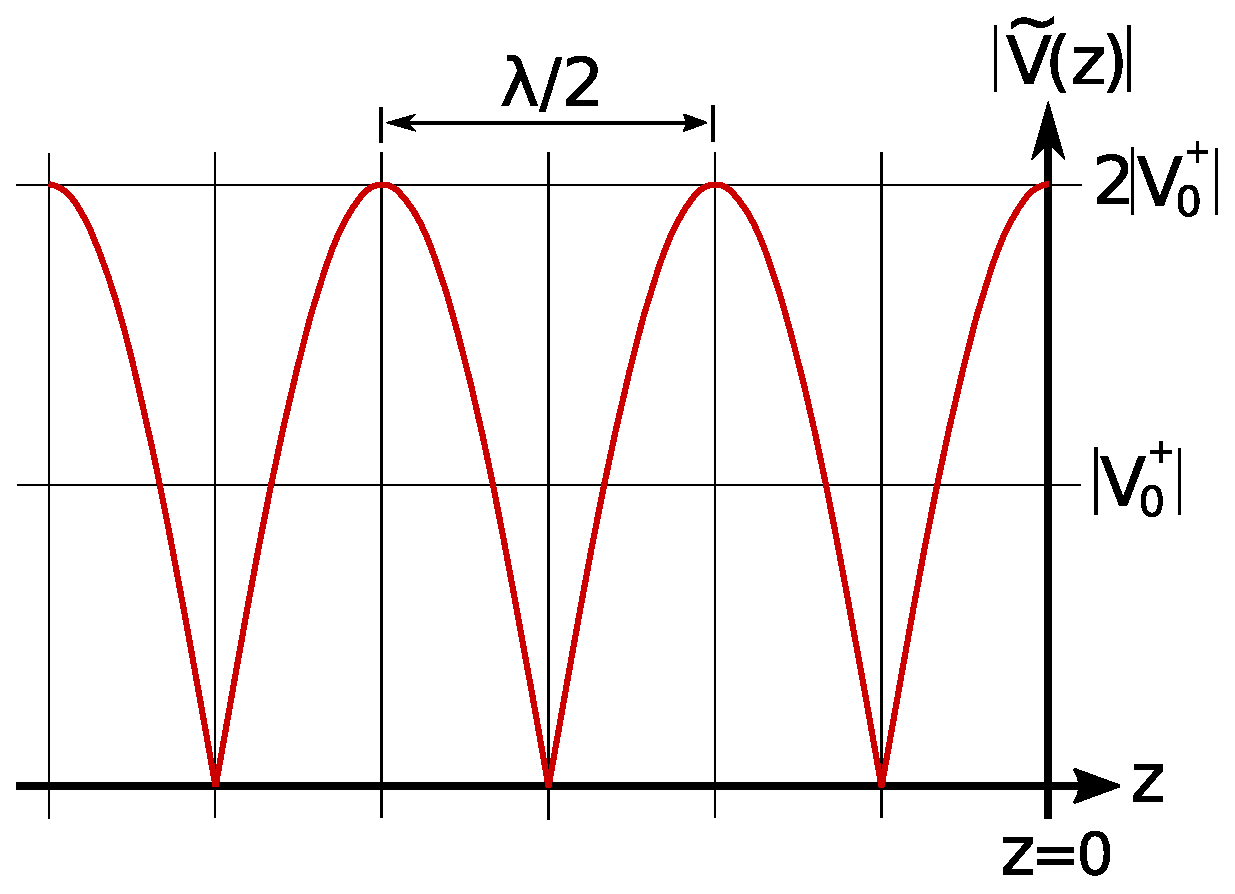
\includegraphics[width=2.5in]{modules/m0086_fStandingWaveOC-V.eps}\\
%}}{The figure shows two plots, one above the other (a and b). Graph (a) shows the potential, with z=0 as the x-axis and the absolute value of the alternating voltage on the y-axis. 
%%The graph depicts a half standing wave, followed by two full standing waves and another half wave. 
%The top peak of the wave reaches twice the absolute value of V super + sub 0, with the absolute value of V super + sub 0 at the midpoint. 
%%Wavelength (lambda) is measured from the peak of the two full peaks. 
%Graph (b) shows the current, and features z=0 on the x-axis and the absolute value of the alternating current on the y-axis. 
%The graph depicts %three full standing waves, with the 
%peaks at twice the absolute value of I super + sub 0. 
%%Wavelength (lambda) is measured from the left minimum of the middle wave to the right minimum of the middle wave. 
%}
(a) Potential.\\~\\
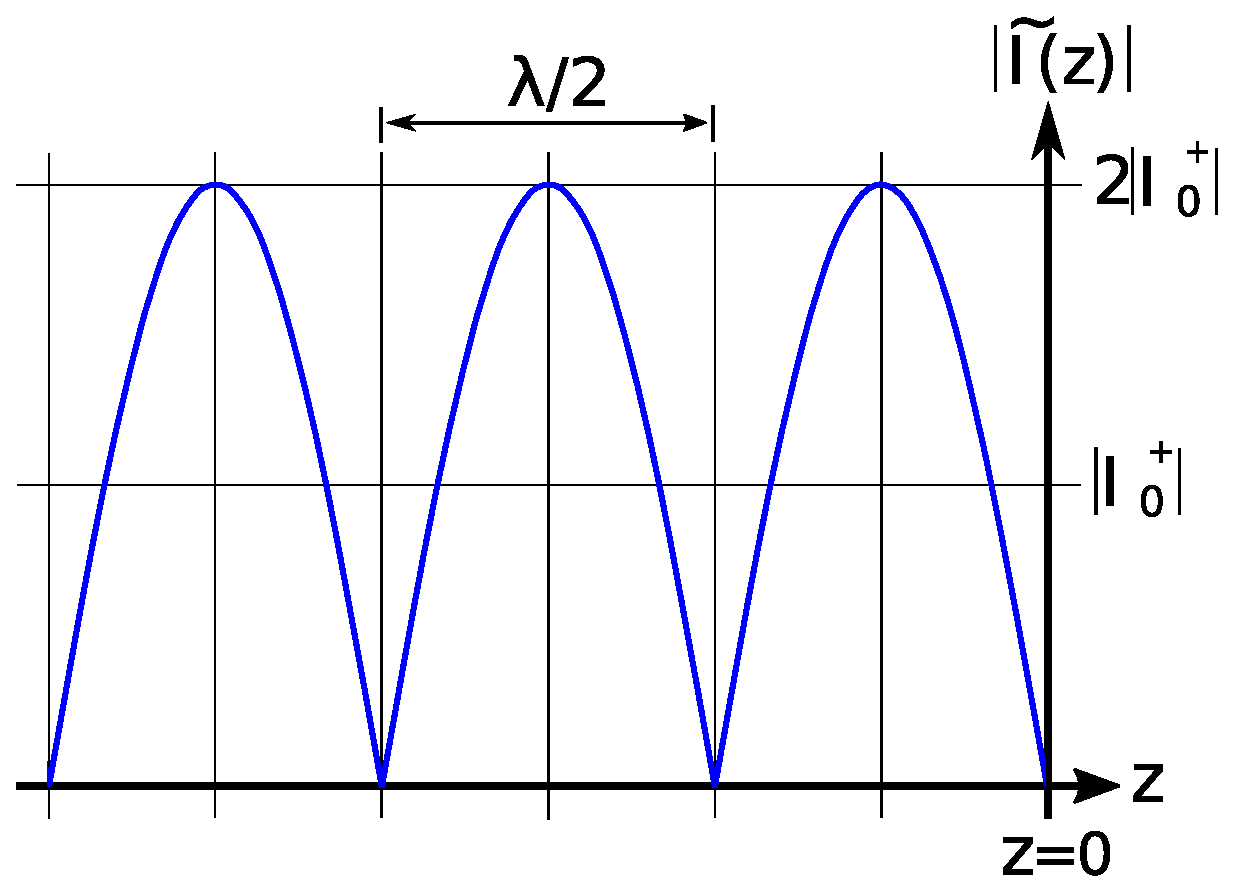
\includegraphics[width=2.5in]{modules/m0086_fStandingWaveOC-C.eps}\\
(b) Current.
\end{center} 
\caption{\label{m0086_fStandingWaveOC}Standing wave associated with an open-circuit termination at $z=0$ (incident wave arrives from left).}
\end{figure} 

Also note: 
%
%ORB HIGHLIGHT
\begin{mdframed}[backgroundcolor=yellow!20,nobreak=true] 
The period of the standing wave is $\lambda/2$; i.e., one-half of a wavelength.
\end{mdframed}
%
This can be confirmed as follows.
First, note that the frequency argument of the cosine function of the standing wave is $2\beta z$.
This can be rewritten as $2\pi\left(\beta/\pi\right)z$, so the frequency of variation is $\beta/\pi$ and the period of the variation is $\pi/\beta$.
Since $\beta=2\pi/\lambda$, we see that the period of the variation is $\lambda/2$.
Furthermore, this is true regardless of the value of $\Gamma$.

{\bf Mismatched loads.} A common situation is that the termination is neither perfectly-matched ($\Gamma=0$) nor an open/short circuit ($\left|\Gamma\right|=1$).
Examples of the resulting standing waves are shown in Figure~\ref{m0086_fStandingWaveExample}. 
%
\begin{figure}
\begin{center}
\pdftooltip{{  % note double braces
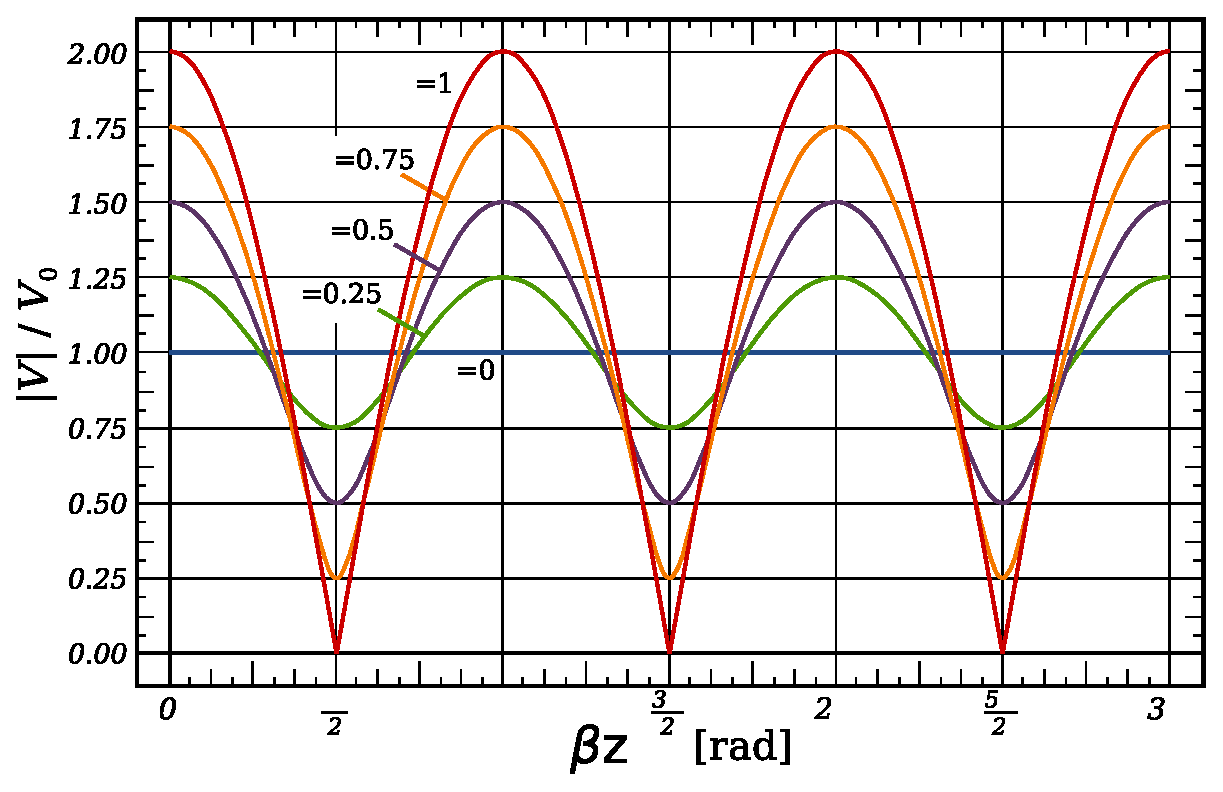
\includegraphics[width=\columnwidth]{modules/m0086_fStandingWaves.eps}
% https://commons.wikimedia.org/wiki/File:Standing_Wave_Ratio.svg
}}{Standing waves plotted: the x-axis (beta sub z) goes from 0 to 3*pi in one-half * pi increments, and the y-axis (absolute value of V divided by V sub 0) goes from 0.00 to 2.00 in 0.25 increments. Each standing wave is a function of gamma. When gamma=0. The wave is flat at 1.00. When gamma=0.25, the peak of the wave reaches 1.25. As gamma increases to 1, the peak increases by 0.25 units each, and the minimum of the waves becomes more pointed. }
\end{center} 
\centerline{\scriptsize 
by~\hyperref[m0086_fStandingWaveExample_Credit]{Inductiveload} (modified) 
%\href{https://creativecommons.org/licenses/by-sa/4.0/}{public domain} 
} 
\caption{
\label{m0086_fStandingWaveExample}
Standing waves associated with loads exhibiting various reflection coefficients.  In this figure the incident wave arrives from the right.
}
\end{figure}

{\bf Additional Reading:}
\begin{itemize}
\item ``\href{https://en.wikipedia.org/wiki/Standing_wave}{Standing Wave}'' on Wikipedia.
\end{itemize}

\index{standing wave|)}


      \vfill\break
    \section{Standing Wave Ratio}
{\color{blue}\tiny[m0081]}      % This is text associated with the open textbook "Open Electromagnetics"
% See immediately below for author, date
% This work is licensed under the Creative Commons Attribution-ShareAlike 4.0 International License. (CC BY-SA 4.0) 
% To view a copy of the license, visit http://creativecommons.org/licenses/by-sa/4.0/

%ORB TITLE Standing Wave Ratio
%ORB AUTHOR 0        # S.W. Ellingson, Virginia Tech (ellingson@vt.edu)
%ORB DATE 20180627   # yyyymmdd
%ORB ABSTRACT Standing wave ratio 

\label{m0081_Standing_Wave_Ratio}  % <-- Must match name of this file and module directory name.  Don't mess with this!
\index{standing wave ratio (SWR)|(}

Precise matching of transmission lines to terminations is often not practical or possible.
Whenever a significant mismatch exists, a standing wave (Section~\ref{m0086_Standing_Waves}) is apparent.
The quality of the match is commonly expressed in terms of the \emph{standing wave ratio} (SWR) of this standing wave. 
%
%ORB HIGHLIGHT
\begin{mdframed}[backgroundcolor=yellow!20,nobreak=true] 
\emph{Standing wave ratio} 
\index{standing wave ratio (SWR)!definition}
(SWR) is defined as the ratio of the maximum magnitude of the standing wave to minimum magnitude of the standing wave.
\end{mdframed}
%
In terms of the potential:
%
\begin{equation}
\boxed{
\mbox{SWR} \triangleq \frac{\mbox{maximum}~|\widetilde{V}|}{\mbox{minimum}~|\widetilde{V}|}
}
\end{equation}  

SWR can be calculated using a simple expression, which we shall now derive. 
In Section~\ref{m0086_Standing_Waves}, we found that:
%
\begin{equation}
\left|\widetilde{V}(z)\right| = |V_0^+| \sqrt{ 1 + \left|\Gamma\right|^2 + 2\left|\Gamma\right| \cos\left( 2\beta z + \phi \right) } 
\end{equation}
%
The maximum value occurs when the cosine factor is equal to $+1$, yielding:
%
\begin{equation}
\mbox{max}~\left|\widetilde{V}\right| 
= |V_0^+| \sqrt{ 1 + \left|\Gamma\right|^2 + 2\left|\Gamma\right| }   
\end{equation}
%
Note that the argument of the square root operator is equal to $\left( 1 + \left|\Gamma\right| \right)^2$; therefore:
%
\begin{equation}
\mbox{max}~\left|\widetilde{V}\right|  
= |V_0^+| \left( 1 + \left|\Gamma\right| \right)
\end{equation}
%
Similarly, the minimum value is achieved when the cosine factor is equal to $-1$, yielding:
%
\begin{equation}
\mbox{min}~\left|\widetilde{V}\right| 
= |V_0^+| \sqrt{ 1 + \left|\Gamma\right|^2 - 2\left|\Gamma\right| }   
\end{equation}
%
So:
%
\begin{equation}
\mbox{min}~\left|\widetilde{V}\right|  
= |V_0^+| \left( 1 - \left|\Gamma\right| \right)
\end{equation}
%
Therefore:
%
\begin{equation}
\boxed{
\mbox{SWR} = \frac{1 + \left|\Gamma\right|}{1 - \left|\Gamma\right|}
}
\label{m0081_eSWR}
\end{equation}

This relationship is shown graphically in Figure~\ref{m0081_fSWRvGamma}. 
Note that SWR ranges from 1 for perfectly-matched terminations ($\Gamma=0$) to infinity for open- and short-circuit terminations ($\left|\Gamma\right|=1$).
%
\begin{figure}
\begin{center}
\pdftooltip{{  % note double braces
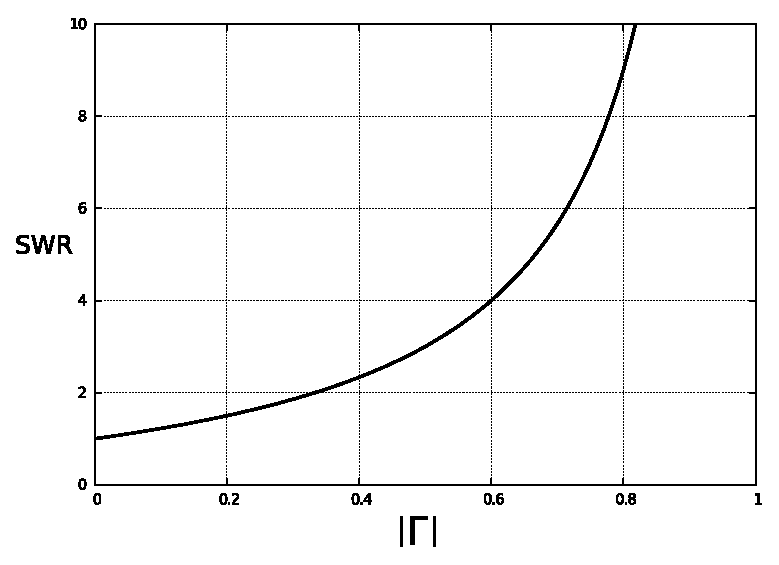
\includegraphics[width=\columnwidth]{modules/m0081_fSWRvGamma.eps}
}}{An x-y graph, with the absolute value of gamma on the x-axis (from 0 to 1) and SWR on the y-axis (from 0 to 10). The plotted curve intersects the y-axis at approximately 1, increasing until it intersects at (0.6, 4). From there, the plotted curve increases more quickly. }
\end{center} 
\caption{\label{m0081_fSWRvGamma}Relationship between SWR and $\left|\Gamma\right|$.}
\end{figure} 

It is sometimes of interest to find the magnitude of the reflection coefficient given SWR.  Solving Equation~\ref{m0081_eSWR} for $\left|\Gamma\right|$ we find:
%
\begin{equation}
\left|\Gamma\right| = \frac{\mbox{SWR}-1}{\mbox{SWR}+1}
\label{m0081_eGammaFromSWR}
\end{equation}
 
SWR is often referred to as the \emph{voltage standing wave ratio} 
\index{voltage standing wave ratio (VSWR)}
(VSWR), although repeating the analysis above for the current reveals that the current SWR is equal to potential SWR, so the term ``SWR'' suffices.
%TODO Problem for students

SWR $<2$ or so is usually considered a ``good match,'' although some applications require SWR $<1.1$ or better, and other applications are tolerant to SWR of 3 or greater.

%ORB EXAMPLE
~\\ \begin{example} 
\begin{mdframed}[backgroundcolor=brown!20,linecolor=brown!20]\raggedright
Reflection coefficient for various values of SWR.
\\~\\
What is the reflection coefficient for the above-cited values of SWR?
Using Equation~\ref{m0081_eGammaFromSWR}, we find:
%
\begin{itemize}
\item SWR = 1.1 corresponds to $\left|\Gamma\right|=0.0476$.
\item SWR = 2.0 corresponds to $\left|\Gamma\right|=1/3$.
\item SWR = 3.0 corresponds to $\left|\Gamma\right|=1/2$.
\end{itemize}
\end{mdframed}\end{example}

\index{standing wave ratio (SWR)|)}


      \vfill\break
    \section{Input Impedance of a Terminated Lossless Transmission Line}
{\color{blue}\tiny[m0087]}      % This is text associated with the open textbook "Open Electromagnetics"
% See immediately below for author, date
% This work is licensed under the Creative Commons Attribution-ShareAlike 4.0 International License. (CC BY-SA 4.0) 
% To view a copy of the license, visit http://creativecommons.org/licenses/by-sa/4.0/

%ORB TITLE Input Impedance of a Terminated Lossless Transmission Line
%ORB AUTHOR 0        # S.W. Ellingson, Virginia Tech (ellingson@vt.edu)
%ORB DATE 20180802   # yyyymmdd
%ORB ABSTRACT Input Impedance of a Terminated Lossless Transmission Line 

\label{m0087_Input_Impedance_of_a_Terminated_Lossless_Transmission_Line} % <-- Must match name of this file and module directory name.  Don't mess with this!
\index{transmission line!input impedance|(}

Consider Figure~\ref{m0087_fZinTerminatedTL}, which shows a lossless transmission line being driven from the left and which is terminated by an impedance $Z_L$ on the right.
If $Z_L$ is equal to the characteristic impedance  $Z_0$ of the transmission line, then the input impedance $Z_{in}$ will be equal to $Z_L$.
Otherwise $Z_{in}$ depends on both $Z_L$ and the characteristics of the transmission line. 
In this section, we determine a general expression for $Z_{in}$ in terms of $Z_L$, $Z_0$, the phase propagation constant $\beta$, and the length $l$ of the line. 
%
\begin{figure}[b!]
\begin{center}
\pdftooltip{{  % note double brace
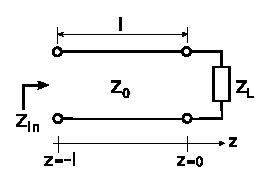
\includegraphics[width=2in]{modules/m0087_fZinTerminatedTL.eps}
}}{A transmission line with two nodes on both the input and output branches. The input node is open and the output node has an impedance labeled Z sub L. Starting at the top left and going clockwise, l is measured between the source terminal and the load terminal. The output of the load is measured at z=0, and the source is at z equal to -l. }
\end{center} 
\caption{\label{m0087_fZinTerminatedTL}A transmission line driven by a source on the left and terminated by an impedance $Z_L$ at $z=0$ on the right.}
\end{figure}   
 
Using the coordinate system indicated in Figure~\ref{m0087_fZinTerminatedTL}, the interface between source and transmission line is located at $z=-l$.  
Impedance 
is defined at the ratio of potential to current, so: 
%
\begin{equation}
Z_{in}(l) \triangleq \frac{\widetilde{V}(z=-l)}{\widetilde{I}(z=-l)} 
\end{equation}
%
Now employing expressions for $\widetilde{V}(z)$ and  $\widetilde{I}(z)$ from Section~\ref{m0086_Standing_Waves} with $z=-l$, we find:
%
\begin{flalign}
Z_{in}(l) &= \frac{V_0^+ \left( e^{+j\beta l} + \Gamma e^{-j\beta l} \right)}{V_0^+ \left( e^{+j\beta l} - \Gamma e^{-j\beta l} \right)/Z_0} \nonumber \\
          &= Z_0 \frac{ e^{+j\beta l} + \Gamma e^{-j\beta l} }{ e^{+j\beta l} - \Gamma e^{-j\beta l} }
\end{flalign}
%
Multiplying both numerator and denominator by $e^{-j\beta l}$:
%
\begin{equation}
\boxed{
Z_{in}(l) = Z_0 \frac{ 1 + \Gamma e^{-j2\beta l} }{  1 - \Gamma e^{-j2\beta l} }
}
\label{m0087_eZin1}
\end{equation}
%
Recall that $\Gamma$ in the above expression is:
%
\begin{equation}
\Gamma = \frac{ Z_L-Z_0 }{  Z_L+Z_0}
\label{m0087_eGamma}
\end{equation}

Summarizing:
%
%ORB HIGHLIGHT
\begin{mdframed}[backgroundcolor=yellow!20,nobreak=true]
Equation~\ref{m0087_eZin1} is the input impedance of a lossless transmission line having characteristic impedance $Z_0$ and which is terminated into a load $Z_L$.  The result also depends on the length and phase propagation constant of the line. 
\end{mdframed}
%
%TODO: PROBLEM: {\color{red}(PROBLEM: SHOW $Z_{in}(l=0)=Z_L$.)}

Note that $Z_{in}(l)$ is periodic in $l$.
Since the argument of the complex exponential factors is $2\beta l$, the frequency at which $Z_{in}(l)$ varies is $\beta/\pi$; and since $\beta=2\pi/\lambda$, the associated period is $\lambda/2$.  
This is very useful to keep in mind because it means that all possible values of $Z_{in}(l)$ are achieved by varying $l$ over $\lambda/2$.  
In other words, changing $l$ by more than $\lambda/2$ results in an impedance which could have been obtained by a smaller change in $l$.
Summarizing to underscore this important idea:
%
%ORB HIGHLIGHT
\begin{mdframed}[backgroundcolor=yellow!20,nobreak=true]
The input impedance of a terminated lossless transmission line is periodic in the length of the transmission line, with period $\lambda/2$.
\end{mdframed}

Not surprisingly, $\lambda/2$ is also the period of the standing wave (Section~\ref{m0086_Standing_Waves}).
This is because -- once again -- the variation with length is due to the interference of incident and reflected waves.

Also worth noting is that Equation~\ref{m0087_eZin1} can be written entirely in terms of $Z_L$ and $Z_0$, since $\Gamma$ depends only on these two parameters.  
Here's that version of the expression:
%
\begin{equation}
Z_{in}(l) = Z_0 \left[ \frac{ Z_L + jZ_0\tan\beta l }{ Z_0 + jZ_L\tan\beta l } \right]
\label{m0087_eZin2}
\end{equation}
%
This expression can be derived by substituting Equation~\ref{m0087_eGamma} into Equation~\ref{m0087_eZin1} and is left as an exercise for the student.
%
%TODO PROBLEM: {\color{red}(PROBLEM: DERIVE ABOVE EQUATION)}

Finally, note that the argument $\beta l$ appearing Equations~\ref{m0087_eZin1} and \ref{m0087_eZin2} has units of radians and is referred to as \emph{electrical length}.
\index{electrical length}
Electrical length can be interpreted as physical length expressed with respect to wavelength and has the advantage that analysis can be made independent of frequency.  

\index{transmission line!input impedance|)}

      \vfill\break
    \section{Input Impedance for Open- and Short-Circuit Terminations}
{\color{blue}\tiny[m0088]}      % This is text associated with the open textbook "Open Electromagnetics"
% See immediately below for author, date
% This work is licensed under the Creative Commons Attribution-ShareAlike 4.0 International License. (CC BY-SA 4.0) 
% To view a copy of the license, visit http://creativecommons.org/licenses/by-sa/4.0/

%ORB TITLE Input Impedance for Open- and Short-Circuit Terminations
%ORB AUTHOR 0        # S.W. Ellingson, Virginia Tech (ellingson@vt.edu)
%ORB DATE 20180802   # yyyymmdd
%ORB ABSTRACT Input Impedance for Open- and Short-Circuit Terminations 

\label{m0088_Input_Impedance_for_Open_and_Short_Circuit_Terminations}  % <-- Must match name of this file and module directory name.  Don't mess with this!
\index{transmission line!input impedance|(}

Let us now consider the input impedance of a transmission line that is terminated in an open- or short-circuit.
Such a transmission line is sometimes referred to as a \emph{stub}.
\index{stub!definition}
\index{transmission line!stub|see{stub}}
First, why consider such a thing?  
From a ``lumped element'' circuit theory perspective, this would not seem to have any particular application.
However, the fact that this structure exhibits an input impedance that depends on length (Section~\ref{m0087_Input_Impedance_of_a_Terminated_Lossless_Transmission_Line}) enables some very useful applications.

First, let us consider the question at hand: 
What is the input impedance when the transmission line is open- or short-circuited? 
For a short circuit, 
\index{short circuit}
\index{stub!short circuit}
$Z_L=0$, $\Gamma=-1$, so we find 
%
\begin{flalign}
Z_{in}(l) &= Z_0 \frac{ 1 + \Gamma e^{-j2\beta l} }{  1 - \Gamma e^{-j2\beta l} } \nonumber \\
          &= Z_0 \frac{ 1 - e^{-j2\beta l} }{  1 + e^{-j2\beta l} } 
\end{flalign}
%
Multiplying numerator and denominator by $e^{+j\beta l}$ we obtain%
\begin{equation}
Z_{in}(l) = Z_0 \frac{ e^{+j\beta l} - e^{-j\beta l} }{  e^{+j\beta l} + e^{-j\beta l} } 
\end{equation}
%
Now we invoke the following trigonometric identities:
%
\begin{flalign}
\cos\theta &= \frac{1}{2}\left[ e^{+j\theta} + e^{-j\theta} \right] \\
\sin\theta &= \frac{1}{j2}\left[ e^{+j\theta} - e^{-j\theta} \right] 
\end{flalign}
%
Employing these identities, we obtain:
%
\begin{equation}
Z_{in}(l) = Z_0 \frac{ j2\left(\sin\beta l\right) }{ 2\left(\cos\beta l\right)  } 
\end{equation}
%
and finally:
%
\begin{equation}
\boxed{
Z_{in}(l) = +jZ_0 \tan \beta l 
}
\label{m0088_eZstubSC}
\end{equation}

Figure~\ref{m0088_fZin}(a) shows what's going on.
As expected, $Z_{in}=0$ when $l=0$, since this amounts to a short circuit with no transmission line.
Also, $Z_{in}$ varies periodically with increasing length, with period $\lambda/2$. This is precisely as expected from standing wave theory (Section~\ref{m0086_Standing_Waves}).
What is of particular interest now is that as $l\rightarrow\lambda/4$, we see $Z_{in}\rightarrow\infty$. Remarkably, the transmission line has essentially transformed the short circuit termination into an open circuit!  
%
\begin{figure}
\begin{center}
\pdftooltip{{  % note double braces
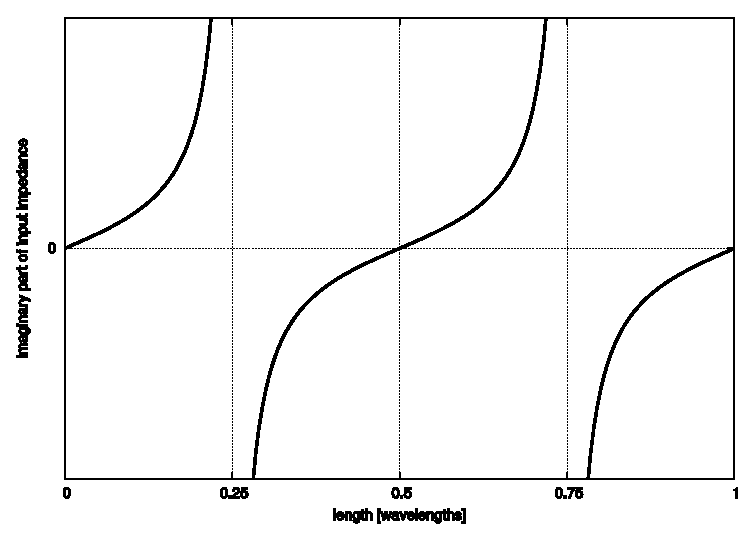
\includegraphics[width=\columnwidth]{modules/m0088_fZinSC.eps}
}}{A plot of the imaginary part of the input impedance (no scale shown) versus length from zero to 1 wavelength.  The plot has the form of the tangent function, with zeros at 0, 0.5, and 1 wavelength and positive asymptotes at 0.25 and 0.75 wavelengths.}\\
(a) Short-circuit termination ($Z_L=0$).\\~\\
\pdftooltip{{  % note double braces
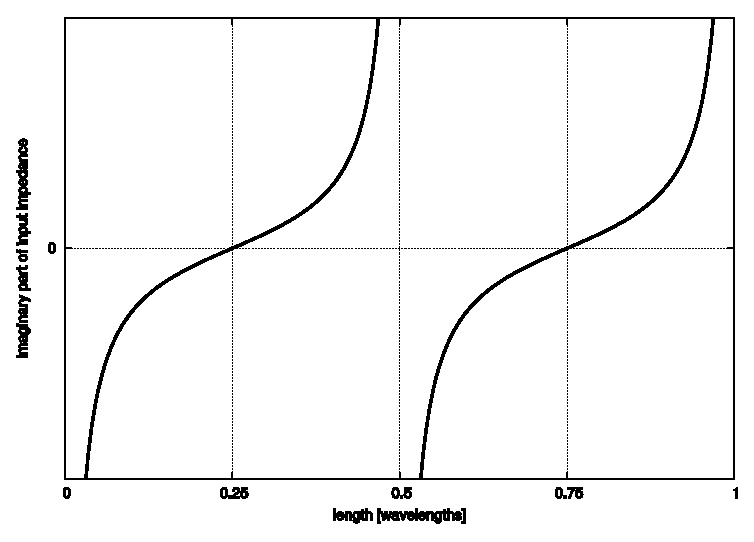
\includegraphics[width=\columnwidth]{modules/m0088_fZinOC.eps}
}}{A plot of the imaginary part of the input impedance (no scale shown) versus length from zero to 1 wavelength.  The plot has the form of the cotangent function, with zeros at 0.25 and 0.75 wavelengths and positive asymptotes at 0.5 and 1 wavelengths.}\\
(b) Open-circuit termination ($Z_L\rightarrow\infty$).
\end{center} 
\caption{\label{m0088_fZin}Input reactance (Im$\left\{Z_{in}\right\}$) of a stub. Re$\left\{Z_{in}\right\}$ is always zero.}
\end{figure}

%------------------------------------------------

For an open circuit 
\index{open circuit}
\index{stub!open circuit}
termination, $Z_L\rightarrow\infty$, $\Gamma=+1$, and we find 
%
\begin{flalign}
Z_{in}(l) &= Z_0 \frac{ 1 + \Gamma e^{-j2\beta l} }{  1 - \Gamma e^{-j2\beta l} } \nonumber \\
          &= Z_0 \frac{ 1 + e^{-j2\beta l} }{  1 - e^{-j2\beta l} } 
\end{flalign}
%
Following the same procedure detailed above for the short-circuit case, we find
%
\begin{equation}
\boxed{
Z_{in}(l) = -jZ_0 \cot \beta l
}
\label{m0088_eZstubOC}
\end{equation}

Figure~\ref{m0088_fZin}(b) shows the result for open-circuit termination.
As expected, $Z_{in}\rightarrow\infty$ for $l=0$, and the same $\lambda/2$ periodicity is observed.
What is of particular interest now is that at $l=\lambda/4$ we see $Z_{in}=0$. In this case, the transmission line has transformed the \emph{open} circuit termination into a \emph{short} circuit.  

Now taking stock of what we have determined:

%ORB HIGHLIGHT
\begin{mdframed}[backgroundcolor=yellow!20,nobreak=true] 
The input impedance of a short- or open-circuited lossless transmission line is completely imaginary-valued and is given by Equations~\ref{m0088_eZstubSC} and \ref{m0088_eZstubOC}, respectively. 
\end{mdframed}

%ORB HIGHLIGHT
\begin{mdframed}[backgroundcolor=yellow!20,nobreak=true] 
The input impedance of a short- or open-circuited lossless transmission line alternates between open- ($Z_{in}\rightarrow\infty$) and short-circuit ($Z_{in}=0$) conditions with each $\lambda/4$-increase in length. 
\end{mdframed}

{\bf Additional Reading:}
\begin{itemize}
\item ``\href{https://en.wikipedia.org/wiki/Stub_(electronics)}{Stub (electronics)}'' on Wikipedia.
\end{itemize}

\index{transmission line!input impedance|)}

      \vfill\break
    \section{Applications of Open- and Short-Circuited Transmission Line Stubs}
{\color{blue}\tiny[m0145]}      % This is text associated with the open textbook "Open Electromagnetics"
% See immediately below for author, date
% This work is licensed under the Creative Commons Attribution-ShareAlike 4.0 International License. (CC BY-SA 4.0) 
% To view a copy of the license, visit http://creativecommons.org/licenses/by-sa/4.0/

%ORB TITLE Applications of Open- and Short-Circuited Transmission Line Stubs
%ORB AUTHOR 0        # S.W. Ellingson, Virginia Tech (ellingson@vt.edu)
%ORB DATE 20180802   # yyyymmdd
%ORB ABSTRACT Applications of Open- and Short-Circuited Transmission Lines

\label{m0145_Applications_of_Open_and_Short-Circuited_Transmission_Lines} % <-- Must match name of this file and module directory name.  Don't mess with this!
\index{stub!applications}

The theory of open- and short-circuited transmission lines -- often referred to as \emph{stubs} -- was addressed in Section~\ref{m0088_Input_Impedance_for_Open_and_Short_Circuit_Terminations}. 
These structures have important and wide-ranging applications. 

In particular, these structures can be used to replace discrete inductors and capacitors in certain applications.  
To see this, consider the short-circuited line (Figure~\ref{m0088_fZin}(b) of Section~\ref{m0088_Input_Impedance_for_Open_and_Short_Circuit_Terminations}). Note that each value of $l$ that is less than $\lambda/4$ corresponds to a particular positive reactance; i.e., the transmission line ``looks'' like an inductor.
Also note that lengths between $\lambda/4$ and $\lambda/2$ result in reactances that are negative; i.e., the transmission line ``looks'' like a capacitor.
Thus, it is possible to replace an inductor or capacitor with a short-circuited transmission line of the appropriate length.
The input impedance of such a transmission line is identical to that of the inductor or capacitor at the design frequency. 
The variation of reactance with respect to frequency will \emph{not} be identical, which may or may not be a concern depending on the bandwidth and frequency response requirements of the application.
Open-circuited lines may be used in a similar way. 

This property of open- and short-circuited transmission lines makes it possible to implement impedance matching 
\index{impedance!matching}
circuits (see Section~\ref{m0094_Single-Stub_Matching}), filters, 
\index{filter}
and other devices entirely from transmission lines, with fewer or no discrete inductors or capacitors required.
Transmission lines do not suffer the performance limitations of discrete devices at high frequencies and are less expensive.
A drawback of transmission line stubs in this application is that the lines are typically much larger than the discrete devices they are intended to replace.

%ORB EXAMPLE
~\\ \begin{example} 
\begin{mdframed}[backgroundcolor=brown!20,linecolor=brown!20]\raggedright
Emitter Induction 
\index{emitter induction}
Using Short-Circuited Line. 
\\~\\
In the design of low-noise amplifiers using bipolar transistors in common-emitter configuration, it is often useful to introduce a little inductance between the emitter and ground.
This is known as ``inductive degeneration,'' ``emitter induction,'' or sometimes by other names.
It can be difficult to find suitable inductors, especially for operation in the UHF band and higher.
However, a microstrip 
\index{microstrip}
line can be used to achieve the desired inductive impedance.
Determine the length of a stub that implements a 2.2~nH inductance at 6~GHz using microstrip line with characteristic impedance $50~\Omega$ and phase velocity $0.6c$. 

{\bf Solution.}
At the design frequency, the impedance looking into this section of line from the emitter should be equal to that of a 2.2~nH inductor, which is 
$+j\omega L = +j2\pi fL = +j82.9~\Omega$.
The input impedance of a short-circuited stub of length $l$ which is grounded (thus, short-circuited) at the opposite end is $+jZ_0\tan\beta l$ (Section~\ref{m0088_Input_Impedance_for_Open_and_Short_Circuit_Terminations}).  
Setting this equal to $+j82.9~\Omega$ and noting that $Z_0=50~\Omega$, we find that $\beta l \cong 1.028$~rad.
The phase propagation constant is (Section~\ref{m0080_Wave_Propagation_on_a_Transmission_Line}):
%
\begin{equation}
\beta = \frac{\omega}{v_p} = \frac{2\pi f}{0.6 c} \cong 209.4~\mbox{rad/m}
\end{equation}
%
Therefore, the length of the microstrip line is $l = \left(\beta l\right) / \beta \cong 4.9$~mm.

\end{mdframed}\end{example}

%%%%%%%%%%%%%%%%%%%%%%%%%%%%%%%%

{\bf Additional Reading:}
\begin{itemize}
\item ``\href{https://en.wikipedia.org/wiki/Stub_(electronics)}{Stub (electronics)}'' on Wikipedia.
\end{itemize}







      \vfill\break
    \section{Measurement of Transmission Line Characteristics}
{\color{blue}\tiny[m0089]}      % This is text associated with the open textbook "Open Electromagnetics"
% See immediately below for author, date
% This work is licensed under the Creative Commons Attribution-ShareAlike 4.0 International License. (CC BY-SA 4.0) 
% To view a copy of the license, visit http://creativecommons.org/licenses/by-sa/4.0/

%ORB TITLE Measurement of Transmission Line Characteristics
%ORB AUTHOR 0        # S.W. Ellingson, Virginia Tech (ellingson@vt.edu)
%ORB DATE 20180802   # yyyymmdd
%ORB ABSTRACT Trick for finding Z_0 by open/short-circuiting line 

\label{m0089_Measurement_of_Transmission_Line_Characteristics} % <-- Must match name of this file and module directory name.  Don't mess with this!
\index{characteristic impedance!measurement}

This section presents a simple technique for measuring the characteristic impedance $Z_0$, electrical length $\beta l$, and phase velocity $v_p$ of a lossless transmission line.
This technique requires two measurements: the input impedance $Z_{in}$ when the transmission line is short-circuited and $Z_{in}$ when the transmission line is open-circuited.

In Section~\ref{m0088_Input_Impedance_for_Open_and_Short_Circuit_Terminations}, it is shown that the input impedance $Z_{in}$ of a short-circuited transmission line is
%
\begin{equation}
Z_{in}^{(SC)} = +jZ_0 \tan\beta l
\nonumber 
\end{equation}
%
and when a transmission line is terminated in an open circuit, the input impedance is
%
\begin{equation}
Z_{in}^{(OC)} = -jZ_0 \cot\beta l 
\nonumber
\end{equation}
%
Observe what happens when we multiply these results together:
%
\begin{equation}
Z_{in}^{(SC)} \cdot Z_{in}^{(OC)} = Z_0^2
\nonumber
\end{equation}
%
that is, the product of the measurements $Z_{in}^{(OC)}$ and  $Z_{in}^{(SC)}$ is simply the square of the characteristic impedance.
Therefore
%
\begin{equation}
Z_0 = \sqrt{ Z_{in}^{(SC)} \cdot Z_{in}^{(OC)} }
\end{equation}
%
If we instead divide these measurements, we find
%
\begin{equation}
\frac{ Z_{in}^{(SC)} }{ Z_{in}^{(OC)} } = -\tan^2\beta l
\nonumber
\end{equation}
%
Therefore:
%
\begin{equation}
\tan\beta l = \left[ - \frac{ Z_{in}^{(SC)} }{ Z_{in}^{(OC)} }  \right]^{1/2}
\end{equation}
%
If $l$ is known in advance to be less than $\lambda/2$, then the electrical length $\beta l$ can be determined by taking the inverse tangent.
\index{electrical length!measurement}
If $l$ is of unknown length and longer than $\lambda/2$, one must take care to account for the periodicity of tangent function; in this case, it may not be possible to unambiguously determine $\beta l$.
Although we shall not present the method here, it is possible to resolve this ambiguity by making multiple measurements over a range of frequencies.

Once $\beta l$ is determined, it is simple to determine $l$ given $\beta$, $\beta$ given $l$, and then $v_p$.  For example, the phase velocity 
\index{phase velocity!measurement}
may be determined by first finding $\beta l$ for a known length using the above procedure, calculating $\beta = \left(\beta l\right)/l$, and then $v_p = \omega/\beta$. 

%%% TODO
% %ORB EXAMPLE
% ~\\ \begin{example} 
% \begin{mdframed}[backgroundcolor=green!20] 
% Measurement of Transmission Line Parameters. 
% \end{mdframed}
% {\color{red}An example of the above procedure.}
% \centerline{\rule{2in}{1pt}} \end{example}


      \vfill\break
    \section{Quarter-Wavelength Transmission Line}
{\color{blue}\tiny[m0091]}      % This is text associated with the open textbook "Open Electromagnetics"
% See immediately below for author, date
% This work is licensed under the Creative Commons Attribution-ShareAlike 4.0 International License. (CC BY-SA 4.0) 
% To view a copy of the license, visit http://creativecommons.org/licenses/by-sa/4.0/

%ORB TITLE Quarter-Wavelength Transmission Line
%ORB AUTHOR 0        # S.W. Ellingson, Virginia Tech (ellingson@vt.edu)
%ORB DATE 20180802   # yyyymmdd
%ORB ABSTRACT Quarter-Wavelength Transmission Line

\label{m0091_Quarter-Wavelength_Transmission_Line} % <-- Must match name of this file and module directory name.  Don't mess with this!
\index{transmission line!quarter-wavelength|(}

Quarter-wavelength sections of transmission line play an important role in many systems at radio and optical frequencies. 
The remarkable properties of open- and short-circuited quarter-wave line are presented in Section~\ref{m0088_Input_Impedance_for_Open_and_Short_Circuit_Terminations} and should be reviewed before reading further.
In this section, we perform a more general analysis, considering not just open- and short-circuit terminations but any terminating impedance, and then we address some applications.

The general expression for the input impedance of a lossless transmission line is (Section~\ref{m0087_Input_Impedance_of_a_Terminated_Lossless_Transmission_Line}):
%
\begin{equation}
Z_{in}(l) = Z_0 \frac{ 1 + \Gamma e^{-j2\beta l} }{  1 - \Gamma e^{-j2\beta l} }
\label{m0093_eZ}
\end{equation}
%
Note that when $l=\lambda/4$:
%
\begin{equation}
2\beta l = 2 \cdot \frac{2\pi}{\lambda} \cdot \frac{\lambda}{4} = \pi 
\nonumber
\end{equation}
%
Subsequently:
%
\begin{equation}
\begin{split}
Z_{in}(\lambda/4) &= Z_0 \frac{ 1 + \Gamma e^{-j\pi} }{  1 - \Gamma e^{-j\pi} } \\
                  &= Z_0 \frac{ 1 - \Gamma }{  1 + \Gamma }
\end{split}
\end{equation}
%
Recall that (Section~\ref{m0087_Input_Impedance_of_a_Terminated_Lossless_Transmission_Line}):
%
\begin{equation}
\Gamma = \frac{Z_L-Z_0}{Z_L+Z_0}
\end{equation}
%
Substituting this expression and then multiplying numerator and denominator by $Z_L+Z_0$, one obtains
%
\begin{equation}
\begin{split}
Z_{in}(\lambda/4) &= Z_0 \frac{ \left( Z_L + Z_0\right) - \left(Z_L - Z_0\right) }{ \left( Z_L + Z_0\right) + \left(Z_L - Z_0\right)  } \\
                  &= Z_0 \frac{ 2Z_0 }{  2Z_L }
\end{split}
\end{equation}
%
Thus,
%
\begin{equation}
\boxed{
Z_{in}(\lambda/4) = \frac{Z_0^2 }{  Z_L }
}
\label{m0091_eQWII}
\end{equation}
%
Note that the input impedance is inversely proportional to the load impedance.
For this reason, a transmission line of length $\lambda/4$ is sometimes referred to as a \emph{quarter-wave inverter} 
\index{quarter-wave inverter}
or simply as a \emph{impedance inverter}.
\index{impedance inverter}

Quarter-wave lines play a very important role in RF engineering.
As impedance inverters, they have the useful attribute of transforming small impedances into large impedances, and vice-versa -- we'll come back to this idea later in this section.
First, let's consider how quarter-wave lines are used for impedance matching.  
Look what happens when we solve Equation~\ref{m0091_eQWII} for $Z_0$:
%
\begin{equation}
Z_0 = \sqrt{Z_{in}(\lambda/4) \cdot Z_L }
\label{m0091_eQWZ0}
\end{equation}
%
This equation indicates that we may match the load $Z_L$ to a source impedance (represented by $Z_{in}(\lambda/4)$) simply by making the characteristic impedance equal to the value given by the above expression and setting the length to $\lambda/4$.
The scheme is shown in Figure~\ref{m0091_fQWM}.
%
\begin{figure}
\begin{center}
\pdftooltip{{  % note double braces
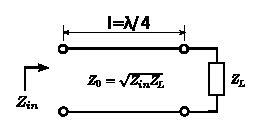
\includegraphics[width=2.5in]{modules/m0091_fQWM.eps}
}}{A transmission line with two nodes on both the input and output branches. Starting at the top left and going clockwise, l equals lambda divided by 4 and is measured between the source terminal and the load terminal.}
\end{center} 
\caption{\label{m0091_fQWM}Impedance-matching using a quarter-wavelength transmission line.}
\end{figure}

%%%%%%%%%%%%%%%%%%%%%%%%%%%%%%%%%%%%%%%%%%%%%%%%%%%%%%%%%%%%%%%

%ORB EXAMPLE
~\\ \begin{example} 
\begin{mdframed}[backgroundcolor=brown!20,linecolor=brown!20]\raggedright
300-to-$50~\Omega$ match using an quarter-wave section of line. 
\\~\\
Design a transmission line segment that matches $300~\Omega$ to $50~\Omega$ at 10~GHz using a quarter-wave match.
Assume microstrip line for which propagation occurs with wavelength 60\% that of free space.

{\bf Solution.}
The line is completely specified given its characteristic impedance $Z_0$ and length $l$.
The length should be one-quarter wavelength with respect to the signal propagating in the line.  
The free-space wavelength $\lambda_0=c/f$ at 10~GHz is $\cong 3$~cm.
Therefore, the wavelength of the signal in the line is $\lambda=0.6\lambda_0\cong 1.8$~cm, 
and the length of the line should be $l=\lambda/4 \cong 4.5$~mm.

The characteristic impedance is given by Equation~\ref{m0091_eQWZ0}:
%
\begin{equation}
Z_0 = \sqrt{ 300~\Omega \cdot 50~\Omega } \cong 122.5~\Omega
\end{equation}
%
This value would be used to determine the width of the microstrip line, as discussed in Section~\ref{m0082_Microstrip_Line}.

\end{mdframed}\end{example}

%%%%%%%%%%%%%%%%%%%%%%%%%%%%%%%%%%%%%%%%%%%%%%%%%%%%%%%%%%%%%%

It should be noted that for this scheme to yield a real-valued characteristic impedance, the product of the source and load impedances must be a real-valued number.  
In particular, this method is \emph{not} suitable if $Z_L$ has a significant imaginary-valued component and matching to a real-valued source impedance is desired.
One possible workaround in this case is the two-stage strategy shown in Figure~\ref{m0091_fQWM2}.
In this scheme, the load impedance is first transformed to a real-valued impedance using a length $l_1$ of transmission line.    This is accomplished using Equation~\ref{m0093_eZ} (quite simple using a numerical search) or using the Smith chart (see ``Additional Reading'' at the end of this section).
The characteristic impedance $Z_{01}$ of this transmission line is not critical and can be selected for convenience.
Normally, the smallest value of $l_1$ is desired.
This value will always be less than $\lambda/4$ since $Z_{in}(l_1)$ is periodic in $l_1$ with period $\lambda/2$; i.e., there are two changes in the sign of the imaginary component of $Z_{in}(l_1)$ as $l_1$ is increased from zero to $\lambda/2$.
After eliminating the imaginary component of $Z_L$ in this manner, the real component of the resulting impedance may then be transformed using the quarter-wave matching technique described earlier in this section. 
%
\begin{figure}
\begin{center}
\pdftooltip{{  % note double braces
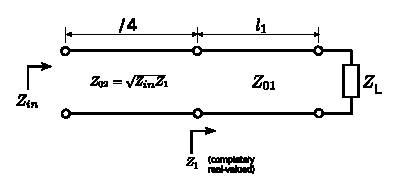
\includegraphics[width=\columnwidth]{modules/m0091_fQWM2.eps}
}}{A transmission line with three sets of parallel nodes extending from input and output branches. Starting at the top left and going clockwise, l equals lambda divided by 4 is measured between the source terminal and the middle terminal. l sub 1 is measured between the middle terminal and the load terminal. Z sub 01 is shown across the terminals on either side of the load. An arrow pointed toward the load originating at the middle terminal on the bottom side is labeled Z sub 1 (completely real-valued). }
\end{center} 
\caption{\label{m0091_fQWM2}Impedance-matching a complex-valued load impedance using quarter-wavelength transmission line.}
\end{figure}

%%%%%%%%%%%%%%%%%%%%%%%%%%%%%%%%%%%%%%%%%%%%%%%%%%%%%

%ORB EXAMPLE
~\\ \begin{example} 
\begin{mdframed}[backgroundcolor=brown!20,linecolor=brown!20]\raggedright
Matching a patch antenna 
\index{antenna!patch}
\index{patch antenna|see{antenna}}
\index{antenna!impedance matching}
to $50~\Omega$.
\\~\\
A particular patch antenna exhibits a source impedance of $Z_A = 35+j35~\Omega$. 
(See ``Microstrip antenna'' in ``Additional Reading'' at the end of this section for some optional reading on patch antennas.) 
Interface this antenna to $50~\Omega$ using the technique described above.
For the section of transmission line adjacent to the patch antenna, use characteristic impedance $Z_{01}=50~\Omega$.
Determine the lengths $l_1$ and $l_2$ of the two segments of transmission line, and the characteristic impedance $Z_{02}$ of the second (quarter-wave) segment. 

{\bf Solution.}
The length of the first section of the transmission line (adjacent to the antenna) is determined using Equation~\ref{m0093_eZ}:
%
\begin{equation}
Z_1(l_1) = Z_{01} \frac{ 1 + \Gamma e^{-j2\beta_1 l_1} }{  1 - \Gamma e^{-j2\beta_1 l_1} }
\end{equation}
%
where $\beta_1$ is the phase propagation constant for this section of transmission line and 
%
\begin{equation}
\Gamma \triangleq \frac{Z_A-Z_{01}}{Z_A+Z_{01}} \cong -0.0059+j0.4142
\end{equation}
%
We seek the value of smallest positive value of $\beta_1 l_1$ for which the imaginary part of $Z_1(l_1)$ is zero.
This can determined using a Smith chart  (see ``Additional Reading'' at the end of this section) or simply by a few iterations of trial-and-error.
Either way we find $Z_1(\beta_1 l_1 = 0.793~\mbox{rad}) \cong 120.719-j0.111~\Omega$, which we deem to be close enough to be acceptable.
Note that $\beta_1 = 2\pi/\lambda$, where $\lambda$ is the wavelength of the signal in the transmission line.
Therefore 
%
\begin{equation}
l_1 
= \frac{\beta_1 l_1}{\beta_1} 
= \frac{\beta_1 l_1}{2\pi} \lambda 
\cong 0.126\lambda
\end{equation} 

The length of the second section of the transmission line, being a quarter-wavelength transformer, should be $l_2 = 0.25\lambda$.
Using Equation~\ref{m0091_eQWZ0}, the characteristic impedance $Z_{02}$ of this section of line should be
%
\begin{equation}
Z_{02} \cong \sqrt{\left(120.719~\Omega\right) \left(50~\Omega\right) } \cong 77.7~\Omega
\end{equation}

%By the way, patch antennas often appear in systems implemented on printed circuit boards, 
%\index{printed circuit board (PCB)}
%because they themselves are easily implemented on printed circuit boards. 
%A great follow-up to this example would be to complete the solution in microstrip (Section~\ref{m0082_Microstrip_Line}) by determining the width of lines given a particular substrate and dielectric thickness.

{\bf Discussion.}
The total length of the matching structure is $l_1+l_2 \cong 0.376\lambda$.
A patch antenna would typically have sides of length about $\lambda/2 = 0.5\lambda$, so the matching structure is nearly as big as the antenna itself.
At frequencies where patch antennas are commonly used, and especially at frequencies in the UHF (300--3000~MHz) band, patch antennas are often comparable to the size of the system, so it is not attractive to have the matching structure also require a similar amount of space.
Thus, we would be motivated to find a smaller matching structure.

\end{mdframed}\end{example}

%%%%%%%%%%%%%%%%%%%%%%%%%%%%%%%%%%%%%%%%%%%%%%%%%%%%

Although quarter-wave matching techniques are generally effective and commonly used, they have one important contraindication, noted above --  They often result in structures that are large. That is, any structure which employs a quarter-wave match will be at least $\lambda/4$ long, and $\lambda/4$ is typically large compared to the associated electronics.  
Other transmission line matching techniques -- and in particular, single stub matching (Section~\ref{m0094_Single-Stub_Matching}) -- typically result in structures which are significantly smaller. 

The impedance inversion property of quarter-wavelength lines has applications beyond impedance matching.  
The following example demonstrates one such application:

%ORB EXAMPLE
~\\ \begin{example} 
\begin{mdframed}[backgroundcolor=brown!20,linecolor=brown!20]\raggedright
RF/DC decoupling in transistor amplifiers.
\index{amplifier}
\\~\\
Transistor amplifiers for RF applications often receive DC current at the same terminal which delivers the amplified RF signal, as shown in Figure~\ref{m0091_BiasT}.
The power supply typically has a low output impedance.
If the power supply is directly connected to the transistor, then the RF will flow predominantly in the direction of the power supply as opposed to following the desired path, which exhibits a higher impedance.
This can be addressed using an inductor in series with the power supply output.
This works because the inductor exhibits low impedance at DC and high impedance at RF.
Unfortunately, discrete inductors are often not practical at high RF frequencies.
This is because practical inductors also exhibit parallel capacitance, which tends to \emph{decrease} impedance.  

A solution is to replace the inductor with a transmission line having length $\lambda/4$ as shown in Figure~\ref{m0091_QWDecoupling}.
A wavelength at DC is infinite, so the transmission line is essentially transparent to the power supply.
At radio frequencies, the line transforms the low impedance of the power supply to an impedance that is very large relative to the impedance of the desired RF path.
Furthermore, transmission lines on printed circuit boards are much cheaper than discrete inductors (and are always in stock!).

\end{mdframed}
%
\begin{figure}
\begin{center}
\pdftooltip{{  % note double braces
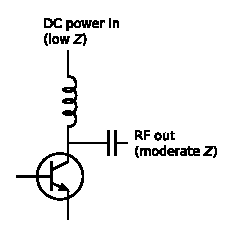
\includegraphics[width=1.5in]{modules/m0091_fBiasT.eps}
}}{A common-emitter RF amplifier in series with an inductor and a capacitor. Starting at the top, the words “DC power in (low Z)” are written above the inductor symbol. Connected at a perpendicular angle is a capacitor, with the words “ RF out (moderate Z)” written directly to the right. Intersection of inductor and capacitor connected to common branch of common-emitter RF amplifier. }
\end{center} 
\caption{\label{m0091_BiasT}Use of an inductor to decouple the DC input power from the RF output signal at the output of a common-emitter RF amplifier.}
\end{figure}
%
\begin{figure}
\begin{center}
\pdftooltip{{  % note double braces
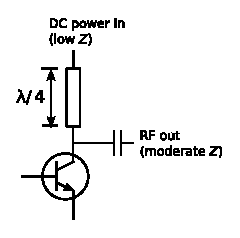
\includegraphics[width=1.5in]{modules/m0091_fQWDecoupling.eps}
}}{Similar layout to a previous figure.  A quarter wavelength transmission line shown as a rectangle. “DC power in (low Z)” is written above the transmission line symbol. Capacitor connected perpendicular “ RF out (moderate Z)” written directly to the right. Shared transmission line-capacitor node connected to common of a common-emitter RF amplifier. }
\end{center} 
\caption{\label{m0091_QWDecoupling}Decoupling of DC input power and RF output signal at the output of a common-emitter RF amplifier, using a quarter-wavelength transmission line.}
\end{figure}
%
\end{example}

%%% TODO Problem ECE3106 17Sp MP2 problem that does the above


{\bf Additional Reading:}
\begin{itemize}
\item ``\href{https://en.wikipedia.org/wiki/Quarter-wave_impedance_transformer}{\small Quarter-wavelength impedance transformer}'' on Wikipedia.
\item ``\href{https://en.wikipedia.org/wiki/Smith_chart}{\small Smith chart}'' on Wikipedia.
\item ``\href{https://en.wikipedia.org/wiki/Microstrip_antenna}{Microstrip antenna}'' on Wikipedia.
\end{itemize}

\index{transmission line!quarter-wavelength|)}

      \vfill\break
    \section{Power Flow on Transmission Lines}
{\color{blue}\tiny[m0090]}      % This is text associated with the open textbook "Open Electromagnetics"
% See immediately below for author, date
% This work is licensed under the Creative Commons Attribution-ShareAlike 4.0 International License. (CC BY-SA 4.0) 
% To view a copy of the license, visit http://creativecommons.org/licenses/by-sa/4.0/

%ORB TITLE Power Flow on Transmission Lines
%ORB AUTHOR 0        # S.W. Ellingson, Virginia Tech (ellingson@vt.edu)
%ORB DATE 20180802   # yyyymmdd
%ORB ABSTRACT Power Flow on Transmission Lines

\label{m0090_Power_Flow_on_Transmission_Lines} % <-- Must match name of this file and module directory name.  Don't mess with this!

It is often important to know the power associated with a wave on a transmission line.
The power of the waves incident upon, reflected by, and absorbed by a load are each of interest.
In this section we shall work out expressions for these powers and consider some implications in terms of the voltage reflection coefficient ($\Gamma$) and standing wave ratio (SWR).
  
Let's begin by considering a lossless transmission line that is oriented along the $z$ axis.
The time-average power associated with a sinusoidal wave having potential $v(z,t)$ and current $i(z,t)$ is
%
\begin{equation}
P_{av}(z) \triangleq \frac{1}{T}\int_{t_0}^{t_0+T}{ v(z,t)~i(z,t)~dt }
\end{equation} 
%
where $T\triangleq 2\pi/f$ is one period of the wave and $t_0$ is the start time for the integration.
Since the time-average power of a sinusoidal signal does not change with time, $t_0$ may be set equal to zero without loss of generality. 

Let us now calculate the power of a wave incident from $z<0$ on a load impedance $Z_L$ at $z=0$.  
We may express the associated potential and current as follows:
%
\begin{equation}
v^+(z,t) = \left|V_0^+\right|\cos\left(\omega t -\beta z +\phi\right)
\end{equation}
%
\begin{equation}
i^+(z,t) = \frac{\left|V_0^+\right|}{Z_0}\cos\left(\omega t -\beta z +\phi\right)
\end{equation}
%
And so the associated time-average power is
%
\begin{equation}
\begin{split}
P_{av}^+(z) &= \frac{1}{T}\int_0^T{ v^+(z,t)~i^+(z,t)~dt } \\
            &= \frac{\left|V_0^+\right|^2}{Z_0} \cdot \frac{1}{T}\int_0^T{ \cos^2\left(\omega t -\beta z +\phi\right) ~dt } 
\end{split}
\label{m0090_ePav1}
\end{equation}
%
Employing a well-known trigonometric identity:
\begin{equation}
\cos^2\theta = \frac{1}{2} + \frac{1}{2}\cos 2\theta 
\end{equation}
we may rewrite the integrand as follows
%
\begin{equation}
\cos^2\left(\omega t -\beta z +\phi\right) = \frac{1}{2} + \frac{1}{2}\cos\left(2\left[\omega t -\beta z +\phi\right]\right) 
\end{equation}
%
Then integrating over both sides of this quantity
%
\begin{equation}
\int_0^T{ \cos^2\left(\omega t -\beta z +\phi\right) ~dt } = \frac{T}{2} + 0 
\end{equation}
%
The second term of the integral is zero because it is the integral of cosine over two complete periods.
Subsequently, we see that the position dependence (here, the dependence on $z$) is eliminated.  
In other words, the power associated with the incident wave is the same for all $z<0$, as expected.
Substituting into Equation~\ref{m0090_ePav1} we obtain:
%
\begin{equation}
\boxed{
P_{av}^+ = \frac{\left|V_0^+\right|^2}{2Z_0} 
}
\label{m0090_ePav+}
\end{equation}
%
This is the time-average power associated with the incident wave, measured at any point $z<0$ along the line.

%ORB HIGHLIGHT
\begin{mdframed}[backgroundcolor=yellow!20,nobreak=true] 
Equation~\ref{m0090_ePav+} gives the time-average power 
\index{transmission line!time-average power}
associated with a wave traveling in a single direction along a lossless transmission line.
\end{mdframed}

Using precisely the same procedure, we find that the power associated with the \emph{reflected} wave is
%
\begin{equation}
P_{av}^- = \frac{\left|\Gamma V_0^+\right|^2}{2Z_0} = \left|\Gamma\right|^2 \frac{\left|V_0^+\right|^2}{2Z_0}
\end{equation}
%
or simply
%
\begin{equation}
\boxed{
P_{av}^- = \left|\Gamma\right|^2 P_{av}^+
}
\label{m0090_ePav-}
\end{equation}

%ORB HIGHLIGHT
\begin{mdframed}[backgroundcolor=yellow!20,nobreak=true] 
Equation~\ref{m0090_ePav-} gives the time-average power associated with the wave reflected from an impedance mismatch.
\end{mdframed}

Now, what is the power $P_L$ delivered to the load impedance $Z_L$?
The simplest way to calculate this power is to use the principle of \emph{conservation of power}.
Applied to the present problem, this principle asserts that the power incident on the load must equal the power reflected plus the power absorbed; i.e.,
%
\begin{equation}
P_{av}^+ = P_{av}^- + P_L
\end{equation}
%
Applying the previous equations we obtain:
%
\begin{equation}
\boxed{
P_L = \left(1-\left|\Gamma\right|^2\right) P_{av}^+
}
\label{m0090_ePL}
\end{equation}

%ORB HIGHLIGHT
\begin{mdframed}[backgroundcolor=yellow!20,nobreak=true] 
Equations~\ref{m0090_ePL} gives the time-average power transferred to a load impedance, and is equal to the difference between the powers of the incident and reflected waves. 
\end{mdframed}

%ORB EXAMPLE
~\\ \begin{example} 
\begin{mdframed}[backgroundcolor=brown!20,linecolor=brown!20]\raggedright
How important is it to match $50~\Omega$ to $75~\Omega$?
\\~\\
Two impedances which commonly appear in radio engineering are $50~\Omega$ and $75~\Omega$.  
It is not uncommon to find that it is necessary to connect a transmission line having a $50~\Omega$ characteristic impedance to a device, circuit, or system having a $75~\Omega$ input impedance, or vice-versa.  If no attempt is made to match these impedances, what fraction of the power will be delivered to the termination, and what fraction of power will be reflected?  What is the SWR?

{\bf Solution.} The voltage reflection coefficient going from $50~\Omega$ transmission line to a $75~\Omega$ load is
%
\begin{equation}
\Gamma = \frac{75-50}{75+50} = +0.2
\nonumber
\end{equation}
%
The fraction of power reflected is $\left|\Gamma\right|^2 = 0.04$, which is 4\%.
The fraction of power transmitted is $1-\left|\Gamma\right|^2$, which is 96\%. 
Going from a $50~\Omega$ transmission line to a $75~\Omega$ termination changes only the sign of $\Gamma$, and therefore, the fractions of reflected and transmitted power remain 4\% and 96\%, respectively.
In either case (from Section~\ref{m0081_Standing_Wave_Ratio}):
%
\begin{equation}
\mbox{SWR} = \frac{1+\left|\Gamma\right|}{1-\left|\Gamma\right|} = 1.5
\nonumber
\end{equation}
%
This is often acceptable, but may not be good enough in some particular applications.
Suffice it to say that it is not necessarily required to use an impedance matching device to connect $50~\Omega$ to $75~\Omega$ devices.
\end{mdframed}\end{example}


      \vfill\break
    \section{Impedance Matching: General Considerations}
{\color{blue}\tiny[m0092]}      % This is text associated with the open textbook "Open Electromagnetics"
% See immediately below for author, date
% This work is licensed under the Creative Commons Attribution-ShareAlike 4.0 International License. (CC BY-SA 4.0) 
% To view a copy of the license, visit http://creativecommons.org/licenses/by-sa/4.0/

%ORB TITLE Impedance Matching: General Considerations
%ORB AUTHOR 0        # S.W. Ellingson, Virginia Tech (ellingson@vt.edu)
%ORB DATE 20180802   # yyyymmdd
%ORB ABSTRACT Preliminary concepts and context for impedance matching 

\label{m0092_Impedance_Matching_General_Considerations} % <-- Must match name of this file and module directory name.  Don't mess with this!
\index{impedance!matching|(}

``Impedance matching'' refers to the problem of transforming a particular impedance $Z_L$ into a modified impedance $Z_{in}$.
The problem of impedance matching arises because it is not convenient, practical, or desirable to have all devices in a system operate at the same input and output impedances.  Here are just a few of the issues:
%
\begin{itemize}
\item It is not convenient or practical to market coaxial cables 
\index{transmission line!coaxial}
having characteristic impedance equal to every terminating impedance that might be encountered.
\item Different types of antennas 
\index{antenna!impedance matching}
operate at different impedances, and the impedance of most antennas vary significantly with frequency.
\item Different types of amplifiers 
\index{amplifier}
operate most effectively at different output impedances.  For example, amplifiers operating as current sources operate most effectively with low output impedance, whereas amplifiers operating as voltage sources operate most effectively with high output impedances.  
\item Independently of the above issue, techniques for the design of transistor amplifiers rely on intentionally \emph{mismatching} impedances; i.e., matching to an impedance different than that which maximizes power transfer or minimizes reflection.  In other words, various design goals are met by applying particular impedances to the input and output ports of the transistor.\footnote{For a concise introduction to this concept, see Chapter~10 of S.W.\ Ellingson, \emph{Radio Systems Engineering}, Cambridge Univ.\ Press, 2016.}
\end{itemize} 
%
For all of these reasons, electrical engineers frequently find themselves with the task of transforming a particular impedance $Z_L$ into a modified impedance $Z_{in}$.

The reader is probably already familiar with many approaches to the impedance matching problem that employ discrete components and do not require knowledge of electromagnetics.\footnote{For an overview, see Chapter~9 of S.W.\ Ellingson, \emph{Radio Systems Engineering}, Cambridge Univ.\ Press, 2016.}  To list just a few of these approaches:  transformers, resistive (lossy) matching, single-reactance matching, and two-reactance (``L'' network) matching.
However, all of these have limitations.
Perhaps the most serious limitations pertain to the performance of discrete components at high frequencies.
Here are just a few of the most common problems:
%
\begin{itemize}
\item Practical resistors actually behave as ideal resistors in series with ideal inductors 
\item Practical capacitors actually behave as ideal capacitors in series with ideal resistors
\item Practical inductors behave as ideal inductors in parallel with ideal capacitors, and in series with ideal resistors.
\end{itemize}
%
All of this makes the use of discrete components increasingly difficult with increasing frequency.

One possible solution to these types of problems is to more precisely model each component, and then to account for the non-ideal behavior by incorporating the appropriate models in the analysis and design process.
Alternatively, one may consider ways to replace particular troublesome components -- or, in some cases, all discrete components -- with transmission line devices.
The latter approach is particularly convenient in circuits implemented on printed circuit boards at frequencies in the UHF band and higher, since the necessary transmission line structures are easy to implement as microstrip 
\index{microstrip}
lines and are relatively compact since the wavelength is relatively small.
However, applications employing transmission lines as components in impedance matching devices can be found at lower frequencies as well.

\index{impedance!matching|)} 

      \vfill\break
    \section{Single-Reactance Matching}
{\color{blue}\tiny[m0093]}      % This is text associated with the open textbook "Open Electromagnetics"
% See immediately below for author, date
% This work is licensed under the Creative Commons Attribution-ShareAlike 4.0 International License. (CC BY-SA 4.0) 
% To view a copy of the license, visit http://creativecommons.org/licenses/by-sa/4.0/

%ORB TITLE Single-Reactance Matching
%ORB AUTHOR 0        # S.W. Ellingson, Virginia Tech (ellingson@vt.edu)
%ORB DATE 20180802   # yyyymmdd
%ORB ABSTRACT Impedance matching using TL to match real part and then discrete impedance to match imaginary part

\label{m00093_Single-Reactance_Matching} % <-- Must match name of this file and module directory name.  Don't mess with this!
\index{impedance!matching|(}

An impedance matching structure can be designed using a section of transmission line combined with a discrete reactance, such as a capacitor or an inductor.
In the strategy presented here, the transmission line is used to transform the real part of the load impedance or admittance to the desired value, and then the reactance is used to modify the imaginary part to the desired value.
(Note the difference between this approach and the quarter-wave technique described in Section~\ref{m0091_Quarter-Wavelength_Transmission_Line}. In that approach, the first transmission line is used to zero the imaginary part.) 
There are two versions of this strategy, which we will now consider separately.

The first version is shown in Figure~\ref{m0093_fSRMs}.
The purpose of the transmission line is to transform the load impedance $Z_L$ into a new impedance $Z_1$ for which Re\{$Z_1$\} $=$ Re\{$Z_{in}$\}.
This can be done by solving the equation (from Section~\ref{m0087_Input_Impedance_of_a_Terminated_Lossless_Transmission_Line})
%
\begin{equation}
\mbox{Re}\left\{Z_1\right\} = \mbox{Re}\left\{Z_0 \frac{ 1 + \Gamma e^{-j2\beta l} }{ 1 - \Gamma e^{-j2\beta l} }\right\}
\label{m0093_eZin}
\end{equation}
%
for $l$, using a numerical search, or using the Smith chart.\footnote{For more about the Smith chart, see ``Additional Reading'' at the end of this section.}
The characteristic impedance 
\index{characteristic impedance}
$Z_0$ 
and phase propagation constant $\beta$ 
of the transmission line are independent variables and can be selected for convenience.
Normally, the smallest value of $l$ that satisfies Equation~\ref{m0093_eZin} is desired.
This value will be $\le\lambda/4$ because the real part of $Z_1$ is periodic in $l$ with period $\lambda/4$.
%
\begin{figure}
\begin{center}
\pdftooltip{{  % note double braces
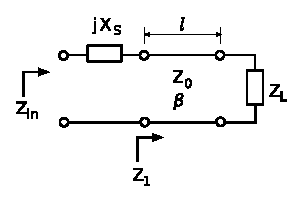
\includegraphics[width=2.5in]{modules/m0093_fSRMs.eps}
}}{A transmission line with three nodes on both the input and output branches. Starting at the top left and going clockwise, a transmission line labeled j * X sub s is between the source terminal and the middle terminal. The length between the middle terminal and the impedance terminal is measured l. Z sub 0 is measured across the terminals on either side of the impedance, with beta underneath. An arrow pointed toward the impedance originating at the middle terminal on the bottom side is labeled Z sub 1.}
\end{center} 
\caption{\label{m0093_fSRMs}Single-reactance matching with a series reactance.}
\end{figure}

After matching the real component of the impedance in this manner, the imaginary component of $Z_1$ may then be transformed to the desired value (Im\{$Z_{in}$\}) by attaching a reactance $X_s$ in series with the transmission line input, yielding $Z_{in} = Z_1 + jX_S$.  Therefore, we choose 
%
\begin{equation}
X_s = \mbox{Im}\left\{Z_{in}-Z_1\right\}
\end{equation}
%
The sign of $X_s$ determines whether this reactance is a capacitor ($X_s<0$) or inductor ($X_s>0$), and the value of this component is determined from $X_s$ and the design frequency.

%ORB EXAMPLE
~\\ \begin{example} 
\label{m0093_eSSR-S}
\begin{mdframed}[backgroundcolor=brown!20,linecolor=brown!20]\raggedright
Single reactance in series.
\\~\\
Design a match consisting of a transmission line in series with a single capacitor or inductor that matches a source impedance of $50\Omega$ to a load impedance of $33.9 + j17.6~\Omega$ at 1.5~GHz. 
The characteristic impedance and phase velocity of the transmission line are $50\Omega$ and $0.6c$ respectively.

{\bf Solution.}
From the problem statement: 
$Z_{in} \triangleq Z_S = 50~\Omega$ and 
$Z_L = 33.9+j17.6~\Omega$ are the source and load impedances respectively at $f=1.5$~GHz.
The characteristic impedance and phase velocity of the transmission line are $Z_0=50~\Omega$ and $v_p=0.6c$ respectively. 

The reflection coefficient $\Gamma$ (i.e., $Z_L$ with respect to the characteristic impedance of the transmission line) is
%
\begin{equation}
\Gamma \triangleq \frac{Z_L - Z_0}{Z_L + Z_0} \cong -0.142 + j0.239
\end{equation} 
%
The length $l$ of the primary line (that is, the one that connects the two ports of the matching structure) is determined using the equation:
%
\begin{equation}
\mbox{Re}\left\{Z_1\right\} = \mbox{Re}\left\{Z_0 \frac{ 1 + \Gamma e^{-j2\beta l} }{ 1 - \Gamma e^{-j2\beta l} }\right\}
\end{equation}
% 
where here
$\mbox{Re}\left\{Z_1\right\}=\mbox{Re}\left\{Z_S\right\}=50~\Omega$.
So a more-specific form of the equation that can be solved for $\beta l$ (as a step toward finding $l$) is:
%
\begin{equation}
1 = \mbox{Re}\left\{ 
           \frac{ 1+\Gamma e^{-j2\beta l } }
                { 1-\Gamma e^{-j2\beta l } } \right\} 
\end{equation}
%
By trial and error (or using the Smith chart if you prefer) we find $\beta l\cong 0.408$~rad for the primary line, yielding $Z_1 \cong 50.0+j29.0~\Omega$ for the input impedance after attaching the primary line.  

We may now solve for $l$ as follows:
Since $v_p = \omega/\beta$ (Section~\ref{m0080_Wave_Propagation_on_a_Transmission_Line}), we find
%
\begin{equation}
\beta = \frac{\omega}{v_p} = \frac{2\pi f}{0.6 c} \cong 52.360~\mbox{rad/m} 
\end{equation}
%
Therefore $l=\left(\beta l\right)/\beta$ $\cong$ \underline{7.8~mm}.

The impedance of the series reactance should be $jX_s \cong -j29.0~\Omega$ to cancel the imaginary part of $Z_1$.
Since the sign of this impedance is negative, it must be a capacitor.
The reactance of a capacitor is $-1/\omega C$, so it must be true that
%
\begin{equation}
-\frac{1}{2\pi f C} \cong -29.0~\Omega
\end{equation}  
%
Thus, we find the series reactance is a \underline{capacitor} of value \underline{$C\cong 3.7$~pF}.
\end{mdframed}\end{example}

\index{admittance|(}
The second version of the single-reactance strategy is shown in Figure~\ref{m0093_fSRMp}.
The difference in this scheme is that the reactance is attached in parallel.
In this case, it is easier to work the problem using admittance (i.e., reciprocal impedance) as opposed to impedance; this is because the admittance of parallel reactances is simply the sum of the associated admittances; i.e., 
%
\begin{equation}
Y_{in} = Y_1 + jB_p
\end{equation}
%
where $Y_{in}=1/Z_{in}$, $Y_1=1/Z_1$, and $B_p$ is the discrete parallel susceptance; 
\index{susceptance}
i.e., the imaginary part of the discrete parallel admittance.
%
\begin{figure}
\begin{center}
\pdftooltip{{  % note double braces
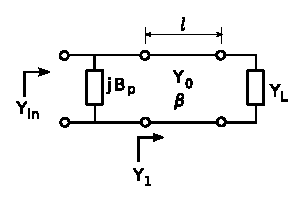
\includegraphics[width=2.5in]{modules/m0093_fSRMp.eps}
}}{A transmission line with three nodes on both the input and output branches. Starting at the top left and going clockwise, a transmission line labeled j times B sub p is connected between the source terminal and the middle terminal in parallel between input and output branches. The length between the middle terminal and the impedance terminal is measured l. Y sub 0 is measured across the terminals on either side of the impedance, with beta underneath. The impedance is labeled Y sub L. An arrow pointed toward the impedance at the middle terminal on the bottom side is labeled Y sub 1.}
\end{center} 
\caption{\label{m0093_fSRMp}Single-reactance matching with a parallel reactance.}
\end{figure}

So, the procedure is as follows.
The transmission line is used to transform $Y_L$ into a new admittance $Y_1$ for which Re\{$Y_1$\} $=$ Re\{$Y_{in}$\}.
First, we note that
%
\begin{equation}
Y_1 \triangleq \frac{1}{Z_1} = Y_0 \frac{ 1 - \Gamma e^{-j2\beta l} }{ 1 + \Gamma e^{-j2\beta l} }
\end{equation}
%
where $Y_0 \triangleq 1/Z_0$ is characteristic \emph{admittance}.
\index{characteristic admittance}
\index{admittance!characteristic|see{characteristic admittance}}
Again, the characteristic impedance $Z_0$ 
and phase propagation constant $\beta$ 
of the transmission line are independent variables and can be selected for convenience.
In the present problem, we aim to solve the equation
%
\begin{equation}
\mbox{Re}\left\{Y_1\right\} = \mbox{Re}\left\{Y_0 \frac{ 1 - \Gamma e^{-j2\beta l} }{ 1 + \Gamma e^{-j2\beta l} }\right\}
\end{equation}
%
for the smallest value of $l$, using a numerical search or using the Smith chart.
After matching the real component of the admittances in this manner, the imaginary component of the resulting admittance may then be transformed to the desired value by attaching the susceptance $B_p$ in parallel with the transmission line input. 
Since we desire $jB_p$ in parallel with $Y_1$ to be $Y_{in}$, the desired value is
%
\begin{equation}
B_p = \mbox{Im}\left\{Y_{in}-Y_1\right\}
\end{equation}
%
The sign of $B_p$ determines whether this is a capacitor ($B_p>0$) or inductor ($B_p<0$), and the value of this component is determined from $B_p$ and the design frequency.

In the following example, we address the same problem raised in Example~\ref{m0093_eSSR-S}, now using the parallel reactance approach:

%ORB EXAMPLE
~\\ \begin{example} 
\label{m0093_eSSR-P}
\begin{mdframed}[backgroundcolor=brown!20,linecolor=brown!20]\raggedright
Single reactance in parallel.
\\~\\
Design a match consisting of a transmission line in parallel with a single capacitor or inductor that matches a source impedance of $50\Omega$ to a load impedance of $33.9 + j17.6~\Omega$ at 1.5~GHz. 
The characteristic impedance and phase velocity of the transmission line are $50\Omega$ and $0.6c$ respectively.

{\bf Solution.}
From the problem statement: 
$Z_{in} \triangleq Z_S = 50~\Omega$ and 
$Z_L = 33.9+j17.6~\Omega$ are the source and load impedances respectively at $f=1.5$~GHz.
The characteristic impedance and phase velocity of the transmission line are $Z_0=50~\Omega$ and $v_p=0.6c$ respectively. 

The reflection coefficient $\Gamma$ (i.e., $Z_L$ with respect to the characteristic impedance of the transmission line) is
%
\begin{equation}
\Gamma \triangleq \frac{Z_L - Z_0}{Z_L + Z_0} \cong -0.142 + j0.239
\end{equation} 
%
The length $l$ of the primary line (that is, the one that connects the two ports of the matching structure) is the solution to:
%
\begin{equation}
\mbox{Re}\left\{Y_1\right\} = \mbox{Re}\left\{Y_{0} \frac{ 1 - \Gamma e^{-j2\beta l} }{ 1 + \Gamma e^{-j2\beta l} }\right\}
\end{equation}
% 
where here
$\mbox{Re}\left\{Y_1\right\}=\mbox{Re}\left\{1/Z_S\right\}=0.02$~mho and 
$Y_0 = 1/Z_0 = 0.02$~mho.
So the equation to be solved for $\beta l$ (as a step toward finding $l$) is:
%
\begin{equation}
1 = \mbox{Re}\left\{ 
           \frac{ 1-\Gamma e^{-j2\beta l } }
                { 1+\Gamma e^{-j2\beta l } } \right\} 
\end{equation}
%
By trial and error (or the Smith chart) we find $\beta l\cong 0.126$~rad for the primary line, yielding $Y_1 \cong 0.0200-j0.0116$~mho for the input admittance after attaching the primary line.  

We may now solve for $l$ as follows:
Since $v_p = \omega/\beta$ (Section~\ref{m0080_Wave_Propagation_on_a_Transmission_Line}), we find
%
\begin{equation}
\beta = \frac{\omega}{v_p} = \frac{2\pi f}{0.6 c} \cong 52.360~\mbox{rad/m} 
\end{equation}
%
Therefore, $l=\left(\beta l\right)/\beta$ $\cong$ \underline{2.4~mm}.

The admittance of the parallel reactance should be $jB_p \cong +j0.0116$~mho to cancel the imaginary part of $Y_1$.
The associated impedance is $1/jB_p \cong -j86.3~\Omega$.
Since the sign of this impedance is negative, it must be a capacitor.
The reactance of a capacitor is $-1/\omega C$, so it must be true that
%
\begin{equation}
-\frac{1}{2\pi f C} \cong -86.3~\Omega
\end{equation}  
%
Thus, we find the parallel reactance is a \underline{capacitor} of value \underline{$C\cong 1.2$~pF}.

\end{mdframed}\end{example}

\index{admittance|)}

Comparing this result to the result from the series reactance method (Example~\ref{m0093_eSSR-S}), we see that the necessary length of transmission line is much shorter, which is normally a compelling advantage.  The tradeoff is that the parallel capacitance is much smaller and an accurate value may be more difficult to achieve.

{\bf Additional Reading:}
\begin{itemize}
\item ``\href{https://en.wikipedia.org/wiki/Smith_chart}{\small Smith chart}'' on Wikipedia.
\end{itemize}

\index{impedance!matching|)}

      \vfill\break
    \section{Single-Stub Matching}
{\color{blue}\tiny[m0094]}      % This is text associated with the open textbook "Open Electromagnetics"
% See immediately below for author, date
% This work is licensed under the Creative Commons Attribution-ShareAlike 4.0 International License. (CC BY-SA 4.0) 
% To view a copy of the license, visit http://creativecommons.org/licenses/by-sa/4.0/

%ORB TITLE Single-Stub Matching
%ORB AUTHOR 0        # S.W. Ellingson, Virginia Tech (ellingson@vt.edu)
%ORB DATE 20180802   # yyyymmdd
%ORB ABSTRACT Single-stub matching.  Refers explicitly to module m0093 (single-reactance matching)

\label{m0094_Single-Stub_Matching} % <-- Must match name of this file and module directory name.  Don't mess with this!
\index{stub!applications|(}
\index{impedance!matching|(}
\index{single-stub matching|(}

In Section~\ref{m00093_Single-Reactance_Matching}, we considered impedance matching schemes consisting of a transmission line combined with a reactance which is placed either in series or in parallel with the transmission line.  
In many problems, the required discrete reactance is not practical because it is not a standard value, or because of non-ideal behavior at the desired frequency (see Section~\ref{m0092_Impedance_Matching_General_Considerations} for more about this), or because one might simply wish to avoid the cost and logistical issues associated with an additional component.
Whatever the reason, a possible solution is to replace the discrete reactance with a transmission line ``stub'' -- that is, a transmission line which has been open- or short-circuited.
Section~\ref{m0088_Input_Impedance_for_Open_and_Short_Circuit_Terminations} explains how a stub can replace a discrete reactance.  
Figure~\ref{m0094_fSSM-SMA} shows a practical implementation of this idea implemented in microstrip.  This section explains the theory, and we'll return to this implementation at the end of the section.
%
\begin{figure}[b!]
\begin{center}
\pdftooltip{{  % note double braces
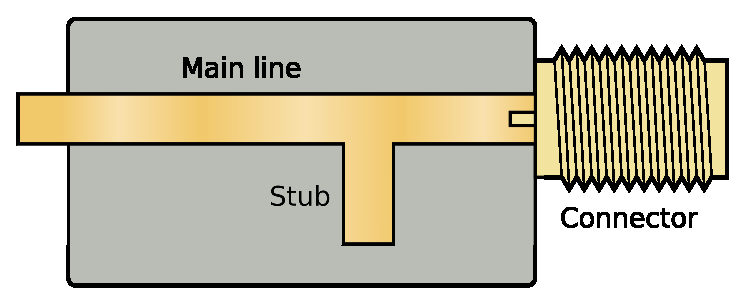
\includegraphics[width=\columnwidth]{modules/m0094_fSSM-SMA.eps}
% https://commons.wikimedia.org/wiki/File:Stripline_stub_matching.svg
}}{A gold-colored microstrip transmission line going through a gray rectangular field. The main line extends horizontally with an arrow inside it pointing to the left to indicate direction. A stub extends downwards perpendicularly from the main line within the gray field. The right end of the main line is capped by a threaded connector outside of the gray field.}
\end{center} 
\centerline{\scriptsize 
\hyperref[m0094_fSSM-SMA_Credit]{Spinningspark} 
\href{https://creativecommons.org/licenses/by-sa/3.0/deed.en}{CC BY~SA 3.0} 
} 
\caption{
\label{m0094_fSSM-SMA}
A practical implementation of a single-stub impedance match using microstrip transmission line.  Here, the stub is open-circuited.
}
\end{figure}

Figure~\ref{m0094_fSSM} shows the scheme.
This scheme is usually implemented using the parallel reactance approach, as depicted in the figure.
Although a series reactance scheme is also possible in principle, it is usually not as convenient.
This is because most transmission lines use one of their two conductors as a local datum; e.g., the ground plane of a printed circuit board for microstrip line is tied to ground, and the outer conductor (``shield'') of a coaxial cable is usually tied to ground.
This is contrast to a discrete reactance (such as a capacitor or inductor), which does not require that either of its terminals be tied to ground.  
This issue is avoided in the parallel-attached stub because the parallel-attached stub and the transmission line to which it is attached \emph{both} have one terminal at ground.
%
\begin{figure}
\begin{center}
\pdftooltip{{  % note double braces
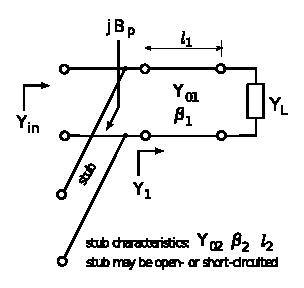
\includegraphics[width=2.5in]{modules/m0094_fSSM.eps}
}}{A transmission line with three nodes on both the input and output branches. Starting at the top left and going clockwise, a stub extending perpendicularly from the input and output terminals is connected between the source terminal and the middle terminal. The length between the middle terminal and the impedance terminal is measured l sub 1. Y sub 01 is measured across the terminals on either side of the impedance, with beta sub 1 underneath. The impedance is labeled Y sub L. An arrow pointed toward the impedance at the middle terminal on the bottom side is labeled Y sub 1. Underneath the graphic are the words "stub characteristics: Y sub 02, beta sub 2, l sub " and "stub may be open- or short-circuited".}
\end{center} 
\caption{\label{m0094_fSSM}Single-stub matching.}
\end{figure}

The single-stub matching procedure is essentially the same as the single parallel reactance method, except the parallel reactance is implemented using a short- or open-circuited stub as opposed a discrete inductor or capacitor.  Since parallel reactance matching is most easily done using admittances, 
\label{admittance}
it is useful to express Equations~\ref{m0088_eZstubSC} and \ref{m0088_eZstubOC} (input impedance of an open- and short-circuited stub, respectively, from Section~\ref{m0088_Input_Impedance_for_Open_and_Short_Circuit_Terminations}) in terms of susceptance:
\index{susceptance}
%
\begin{equation}
B_p = -Y_{02} \cot\left(\beta_2 l_2\right) ~~\mbox{short-circuited stub}
\end{equation}
%
\begin{equation}
B_p = +Y_{02} \tan\left(\beta_2 l_2\right) ~~\mbox{open-circuited stub}
\end{equation}
%
As in the main line, the characteristic impedance $Z_{02}=1/Y_{02}$ is an independent variable and is chosen for convenience.

A final question is when should you use a short-circuited stub, and when should you use an open-circuited stub?
Given no other basis for selection, the termination that yields the shortest stub is chosen.
An example of an ``other basis for selection'' that frequently comes up is whether DC might be present on the line. If DC is present with the signal of interest, then a short circuit termination without some kind of remediation to prevent a short circuit for DC would certainly be a bad idea.

In the following example we address the same problem raised in Section~\ref{m00093_Single-Reactance_Matching} (Examples~\ref{m0093_eSSR-S} and \ref{m0093_eSSR-P}), now using the single-stub approach:
~\\
%
%ORB EXAMPLE
~\\ \begin{example} 
\begin{mdframed}[backgroundcolor=brown!20,linecolor=brown!20]\raggedright
Single stub matching.
\\~\\
% This is from HW9 of ECE3106 15Fa
Design a single-stub match that matches a source impedance of $50\Omega$ to a load impedance of $33.9 + j17.6~\Omega$. %at 1.5~GHz. 
Use transmission lines having characteristic impedances of $50\Omega$ throughout, and leave your answer in terms of wavelengths.

{\bf Solution.}
From the problem statement: $Z_{in} \triangleq Z_S = 50~\Omega$ and $Z_L = 33.9+j17.6~\Omega$ are the source and load impedances respectively.
$Z_0=50~\Omega$ is the characteristic impedance of the transmission lines to be used.
The reflection coefficient $\Gamma$ (i.e., $Z_L$ with respect to the characteristic impedance of the transmission line) is
%
\begin{equation}
\Gamma \triangleq \frac{Z_L - Z_0}{Z_L + Z_0} \cong -0.142 + j0.239
\end{equation} 
%
The length $l_1$ of the primary line (that is, the one that connects the two ports of the matching structure) is the solution to the equation (from Section~\ref{m00093_Single-Reactance_Matching}):
%
\begin{equation}
\mbox{Re}\left\{Y_1\right\} = \mbox{Re}\left\{Y_{01} \frac{ 1 - \Gamma e^{-j2\beta_1 l_1} }{ 1 + \Gamma e^{-j2\beta_1 l_1} }\right\}
\end{equation}
% 
where here
$\mbox{Re}\left\{Y_1\right\}=\mbox{Re}\left\{1/Z_S\right\}=0.02$~mho and 
$Y_{01} = 1/Z_0 = 0.02$~mho.
Also note
%
\begin{equation}
2\beta_1 l_1 = 2 \left(\frac{2\pi}{\lambda}\right) l_1 = 4\pi \frac{l_1}{\lambda}
\end{equation}
%
where $\lambda$ is the wavelength in the transmission line.
So the equation to be solved for $l_1$ is:
%
\begin{equation}
1 = \mbox{Re}\left\{ 
           \frac{ 1-\Gamma e^{-j4\pi l_1/\lambda } }
                { 1+\Gamma e^{-j4\pi l_1/\lambda } } \right\} 
\end{equation}
%
By trial and error (or using the Smith chart; see ``Additional Reading'' at the end of this section) we find \underline{$l_1\cong 0.020\lambda$} for the primary line, yielding $Y_1 \cong 0.0200-j0.0116$~mho for the input admittance after attaching the primary line.  

We now seek the shortest stub having an input admittance of $\cong +j0.0116$~mho to cancel the imaginary part of $Y_1$.  
For an open-circuited stub, we need
%
\begin{equation}
B_p = +Y_0 \tan{2\pi l_2/\lambda} \cong +j0.0116~\mbox{mho}
\end{equation}
%
The smallest value of $l_2$ for which this is true is $\cong 0.084\lambda$.  
For a short-circuited stub, we need
%
\begin{equation}
B_p = -Y_0 \cot{2\pi l_2/\lambda} \cong +j0.0116~\mbox{mho}
\end{equation}
%
The smallest positive value of $l_2$ for which this is true is $\cong 0.334\lambda$; i.e., much longer.  
Therefore, we choose the \underline{open-circuited stub} with \underline{$l_2\cong 0.084\lambda$}.  
Note the stub is attached in parallel at the source end of the primary line.

\end{mdframed}\end{example}

%Finally, returning to Figure~\ref{m0094_fSSM-SMA}, 
Single-stub matching is a very common method for impedance matching using microstrip lines at frequences in the UHF band (300-3000~MHz) and above.  In Figure~\ref{m0094_fSSM-SMA}, the top (visible) traces comprise one conductor, whereas the ground plane (underneath, so not visible) comprises the other conductor.  The end of the stub is not connected to the ground plane, so the termination is an open circuit.  A short circuit termination is accomplished by connecting the end of the stub to the ground plane using a \emph{via}; that is, a plated-through that electrically connects the top and bottom layers.

%%%%%%%%%%%%%%%%%%%%%%%%%%%%%%%%%%

{\bf Additional Reading:}
\begin{itemize}
\item ``\href{https://en.wikipedia.org/wiki/Stub_(electronics)}{Stub (electronics)}'' on Wikipedia.
\item ``\href{https://en.wikipedia.org/wiki/Smith_chart}{\small Smith chart}'' on Wikipedia.
\item ``\href{https://en.wikipedia.org/wiki/Via_(electronics)}{Via (electronics)}'' on Wikipedia.
\end{itemize}

\index{stub!applications|)}
\index{impedance!matching|)}
\index{single-stub matching|)}

      \vfill\break
{\color{blue}\tiny[m0151]}    % This is text associated with the open textbook "Open Electromagnetics"
% See immediately below for author, date
% This work is licensed under the Creative Commons Attribution-ShareAlike 4.0 International License. (CC BY-SA 4.0) 
% To view a copy of the license, visit http://creativecommons.org/licenses/by-sa/4.0/

%ORB TITLE Transmission Lines
%ORB AUTHOR 0        # S.W. Ellingson, Virginia Tech (ellingson@vt.edu)
%ORB DATE 20180701   # yyyymmdd
%ORB ABSTRACT End matter for chapter entitled "Transmission Lines"

\label{m0151_Ch_End_Matter_Transmission_Lines} % <-- Must match name of this file and module directory name.  Don't mess with this!

\onecolumn
\section*{Image Credits}

\begin{itemize}

\item[Fig.] \label{m0028_fPoorTL_Credit}
  \ref{m0028_fPoorTL}:
  Dmitry G, 
  {\footnotesize \url{https://en.wikipedia.org/wiki/File:Mastech_test_leads.JPG}},\\ 
  public domain.

\item[Fig.] \label{m0028_fCoax_Credit}
  \ref{m0028_fCoax}:
  \copyright~Tkgd2007, 
  \url{https://commons.wikimedia.org/wiki/File:Coaxial_cable_cutaway.svg},\\ 
  CC BY 3.0 (\url{https://creativecommons.org/licenses/by/3.0/}).\\
  Minor modifications from the original.

\item[Fig.] \label{m0028_fMicrostrip_Credit}
  \ref{m0028_fMicrostrip}:
  \copyright~SpinningSpark, 
  \url{https://en.wikipedia.org/wiki/File:Microstrip_structure.svg},\\ 
  CC BY~SA 3.0 (\url{https://creativecommons.org/licenses/by-sa/3.0/}).\\
  Minor modifications from the original.

\item[Fig.] \label{m0028_fWaveGuide_Credit}
  \ref{m0028_fWaveGuide}:
  \copyright~Averse, 
  \url{https://en.wikipedia.org/wiki/File:Diplexer1.jpg},\\ 
  CC BY~SA 2.0 Germany (\url{https://creativecommons.org/licenses/by-sa/2.0/de/deed.en}).

\item[Fig.] \label{m0028_fOpticalFiber_Credit}
  \ref{m0028_fOpticalFiber}:
  \copyright~BigRiz, 
  \url{https://en.wikipedia.org/wiki/File:Fibreoptic.jpg},\\ 
  CC BY~SA 3.0 Unported (\url{https://creativecommons.org/licenses/by-sa/3.0/deed.en}).

\item[Fig.] \label{m0077_fTransmission_line_symbols_Credit}
  \ref{m0077_fTransmission_line_symbols}:
  \copyright~Omegatron, 
  \url{https://commons.wikimedia.org/wiki/File:Transmission_line_symbols.svg},\\ 
  CC BY~SA 3.0 Unported (\url{https://creativecommons.org/licenses/by-sa/3.0/deed.en}).\\
  Modified.

\item[Fig.] \label{m0029_fLumpedElementModel_Credit}
  \ref{m0029_fLumpedElementModel}:
  \copyright~Omegatron, 
  \url{https://commons.wikimedia.org/wiki/File:Transmission_line_element.svg},\\ 
  CC BY~SA 3.0 Unported (\url{https://creativecommons.org/licenses/by-sa/3.0/deed.en}).\\
  Modified.

\item[Fig.] \label{m0079_fLumpedElementModel_Credit}
  \ref{m0079_fLumpedElementModel}:
  \copyright~Omegatron, 
  \url{https://commons.wikimedia.org/wiki/File:Transmission_line_element.svg},\\ 
  CC BY~SA 3.0 Unported (\url{https://creativecommons.org/licenses/by-sa/3.0/deed.en}).\\
  Modified.

\item[Fig.] \label{m0143_fRG-59_Credit}
  \ref{m0143_fRG-59}:
  \copyright~Arj, 
  \url{https://en.wikipedia.org/wiki/File:RG-59.jpg},\\ 
  CC BY~SA 3.0 Unported (\url{https://creativecommons.org/licenses/by-sa/3.0/deed.en}).

\item[Fig.] \label{m0082_fMicrostripCrossSection_Credit}
  \ref{m0082_fMicrostripCrossSection}:
  \copyright~7head7metal7, 
  \url{https://commons.wikimedia.org/wiki/File:Microstrip_scheme.svg},\\ 
  CC BY~SA 3.0 (\url{https://creativecommons.org/licenses/by-sa/3.0/}).\\
  Minor modifications from the original.

\item[Fig.] \label{m0086_fStandingWaveExample_Credit}
  \ref{m0086_fStandingWaveExample}:
  by~Inductiveload, 
  \url{https://commons.wikimedia.org/wiki/File:Standing_Wave_Ratio.svg},\\ 
  public domain.\\
  Modifications from the original.

\item[Fig.] \label{m0094_fSSM-SMA_Credit}
  \ref{m0094_fSSM-SMA}:
  \copyright~Spinningspark, 
  \url{https://commons.wikimedia.org/wiki/File:Stripline_stub_matching.svg},\\ 
  CC BY~SA 3.0 (\url{https://creativecommons.org/licenses/by-sa/3.0/}).\\
  Minor modifications from the original: curly braces deleted.

\end{itemize}

\twocolumn

  \chapter{Vector Analysis}
  \thispagestyle{fancy} % override footer in first page of chapter
  \fancyhf{}            % reset header and footer
  \fancyfoot[C]{\footnotesize \emph{Electromagnetics Vol~1}. ~\copyright~2018 S.W.\ Ellingson ~CC~BY~SA~4.0. ~\url{https://doi.org/10.21061/electromagnetics-vol-1}}
    \section{Vector Arithmetic}
{\color{blue}\tiny[m0006]}      % This is text associated with the open textbook "Open Electromagnetics"
% See immediately below for author, date
% This work is licensed under the Creative Commons Attribution-ShareAlike 4.0 International License. (CC BY-SA 4.0) 
% To view a copy of the license, visit http://creativecommons.org/licenses/by-sa/4.0/

%ORB TITLE Vector Arithmetic
%ORB AUTHOR 0        # S.W. Ellingson, Virginia Tech (ellingson@vt.edu)
%ORB DATE 20180803   # yyyymmdd
%ORB ABSTRACT Vector Arithmetic

\label{m0006_Vector_Arithmetic} % <-- Must match name of this file and module directory name.  Don't mess with this!
\index{vector!arithmetic|(}

A \emph{vector} 
\index{vector!definition}
is a mathematical object that has both a scalar part (i.e., a magnitude and possibly a phase), as well as a direction.
Many physical quantities are best described as vectors.
For example, the rate of movement through space can be described as \emph{speed}; i.e., as a scalar having SI base units of m/s.
However, this quantity is more completely described as \emph{velocity}; 
\index{velocity}
i.e., as a vector whose scalar part is speed and direction indicates the direction of movement.
Similarly, force 
\index{force}
is a vector whose scalar part indicates magnitude (SI base units of N), and direction indicates the direction in which the force is applied.
Electric and magnetic fields are also best described as vectors. 

In mathematical notation, a real-valued vector ${\bf A}$ is said to have a magnitude $A=\left|{\bf A}\right|$ and direction $\hat{\bf a}$ such that
%
\begin{equation}
{\bf A} = A \hat{\bf a}
\end{equation}
%
where $\hat{\bf a}$ is a unit vector 
\index{unit vector}
\index{vector!unit}
(i.e., a real-valued vector having magnitude equal to one) having the same direction as ${\bf A}$.
If a vector is complex-valued, then $A$ is similarly complex-valued.

{\bf Cartesian Coordinate System.} 
\index{Cartesian coordinate system}
Fundamentals of vector arithmetic are most easily grasped using the Cartesian coordinate system.
This system is shown in Figure~\ref{m0006_fCartesian}.
Note carefully the relative orientation of the $x$, $y$, and $z$ axes.
This orientation is important. 
For example, there are two directions that are perpendicular to the $z=0$ plane (in which the $x$- and $y$-axes lie), but the $+z$ axis is specified to be one of these in particular.  
%
\begin{figure}
\begin{center}
\pdftooltip{{  % note double brac
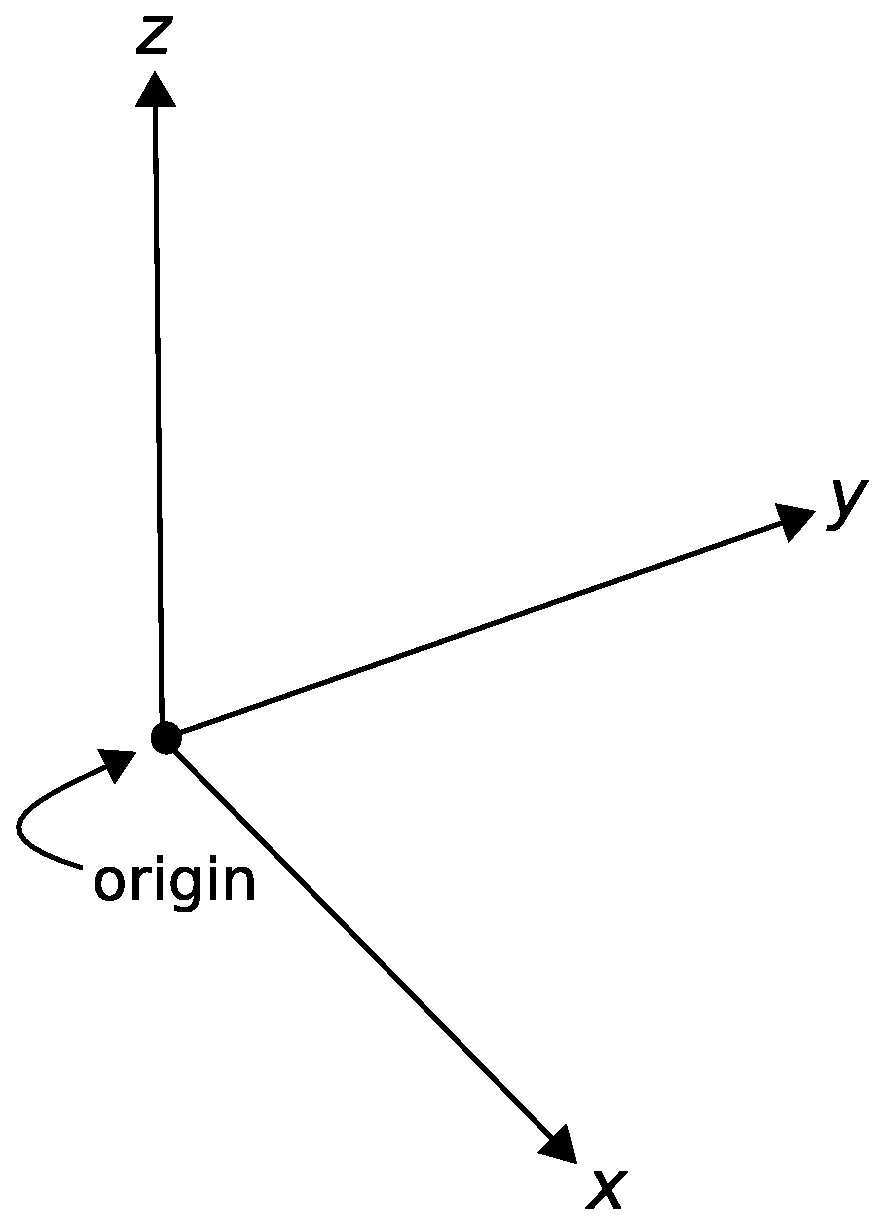
\includegraphics[width=1.5in]{modules/m0006_fCartesian.eps} 
% https://commons.wikimedia.org/wiki/File:M0006_fCartesian.svg
}}{x, y, and z axes. The z-axis points vertically. The y-axis and x-axis are perpendicular to the z-axis and to one another. They are connected at the origin.}
\end{center}
\centerline{\scriptsize 
\copyright~\hyperref[m0006_fCartesian_Credit]{K.\ Kikkeri} 
\href{https://creativecommons.org/licenses/by-sa/4.0/}{CC BY~SA 4.0} 
} 
\caption{
\label{m0006_fCartesian}
Cartesian coordinate system.
}
\end{figure}

{\bf Position-Fixed vs. Position-Free Vectors.} 
\index{vector!position-fixed}
\index{vector!position-free}
It is often convenient to describe a position in space as a vector for which the magnitude is the distance from the origin of the coordinate system and for which the direction is measured from the origin toward the position of interest.
This is shown in Figure~\ref{m0006_fPositionFixed}.
These \emph{position vectors} are ``position-fixed'' in the sense that they are defined with respect to a single point in space, which in this case is the origin.  Position vectors can also be defined as vectors that are defined with respect to some other point in space, in which case they are considered position-fixed to that position.
%
\begin{figure}
\begin{center}
\pdftooltip{{  % note double braces
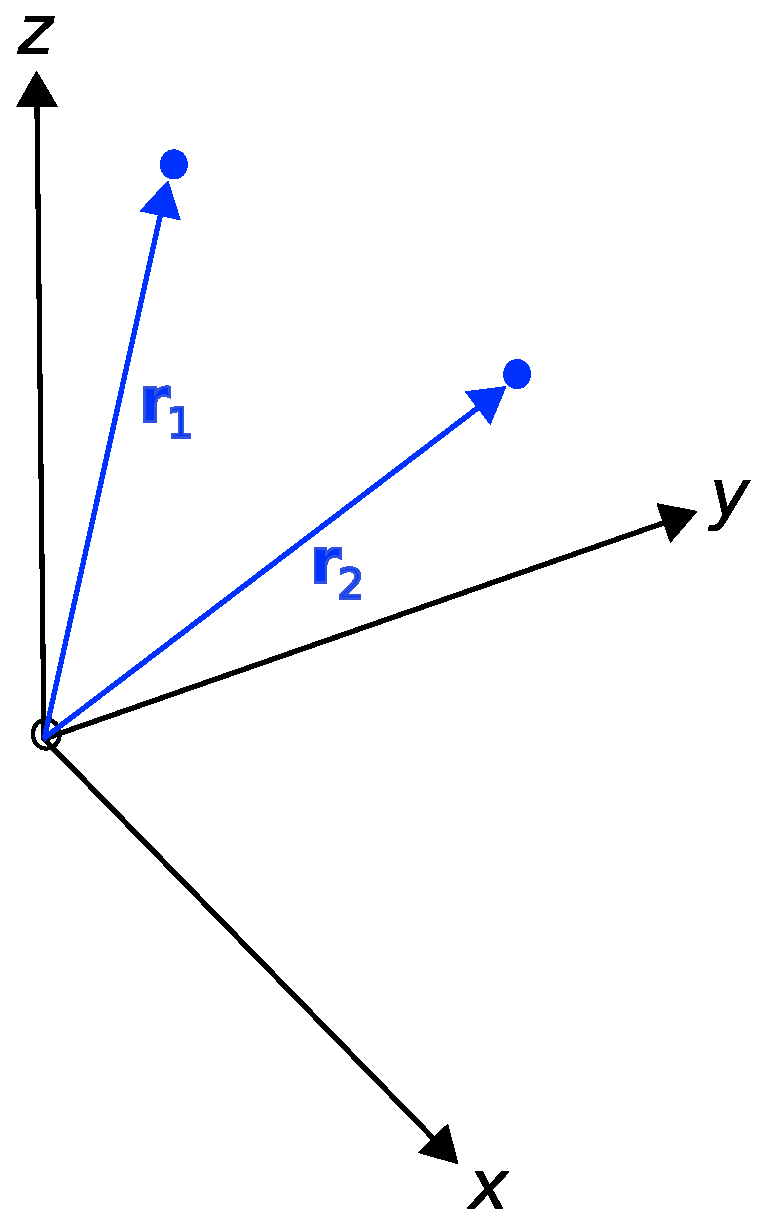
\includegraphics[width=1.5in]{modules/m0006_fPositionFixed.eps}
% https://commons.wikimedia.org/wiki/File:M0006_fPositionFixed.svg
}}{The same Cartesian coordinate system shown in a previous figure. Two blue points are arbitrarily plotted in the 3D space. There is a blue arrow pointing to each of the points from the origin. These represent vectors r sub 1 and r sub 2.}
\end{center} 
\centerline{\scriptsize 
\copyright~\hyperref[m0006_fPositionFixed_Credit]{K.\ Kikkeri} 
\href{https://creativecommons.org/licenses/by-sa/4.0/}{CC BY~SA 4.0} 
} 
\caption{
\label{m0006_fPositionFixed}
Position vectors. The vectors ${\bf r}_1$ and ${\bf r}_1$ are position-fixed and refer to particular locations.
}
\end{figure}

\emph{Position-free} vectors, on the other hand, are not defined with respect to a particular point in space.  
An example is shown in Figure~\ref{m0006_fPositionFree}.
Particles 1~m apart may both be traveling at 2~m/s in the same direction.  
In this case, the velocity of each particle can be described using the same vector, even though the particles are located at different points in space. 
%
\begin{figure}
\begin{center}
\pdftooltip{{  % note double braces
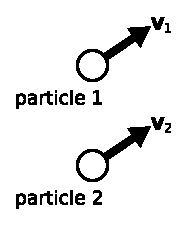
\includegraphics[width=1in]{modules/m0006_fPositionFree.eps}
% https://commons.wikimedia.org/wiki/File:M0006_fPositionFree.svg
}}{Two diagrams, one below the other. The top diagram shows an arrow of arbitrary length and direction pointing out of an empty circle. This arrow is labeled v sub 1 and the empty circle is particle 1. The bottom diagram is identical except the arrow is labeled v sub 2  and the empty circle is particle 2.}
\end{center} 
\centerline{\scriptsize 
\copyright~\hyperref[m0006_fPositionFree_Credit]{K.\ Kikkeri} 
\href{https://creativecommons.org/licenses/by-sa/4.0/}{CC BY~SA 4.0} 
} 
\caption{
\label{m0006_fPositionFree}
Two particles exhibiting the same velocity.  In this case, the velocity vectors ${\bf v}_1$ and ${\bf v}_2$ are position-free and equal.
}
\end{figure}

Position-free vectors are said to be equal if they have the same magnitudes and directions.
Position-fixed vectors, on the other hand, must also be referenced to the same position (e.g., the origin) to be considered equal.

{\bf Basis Vectors.} 
Each coordinate system is defined in terms of three basis vectors which concisely describe all possible ways to traverse three-dimensional space. 
A basis vector is a position-free unit vector that is perpendicular to all other basis vectors for that coordinate system. 
The basis vectors $\hat{\bf x}$, $\hat{\bf y}$, and $\hat{\bf z}$ of the Cartesian coordinate system are shown in Figure~\ref{m0006_fCartesianBasis}. 
In this notation, $\hat{\bf x}$ indicates the direction in which $x$ increases most rapidly, $\hat{\bf y}$ indicates the direction in which $y$ increases most rapidly, and $\hat{\bf z}$ indicates the direction in which $z$ increases most rapidly.
Alternatively, you might interpret $\hat{\bf x}$, $\hat{\bf y}$, and $\hat{\bf z}$ as unit vectors that are parallel to the $x$-, $y$-, and $z$-axes and point in the direction in which values along each axis increase.
%
\begin{figure}
\begin{center}
\pdftooltip{{  % note double braces
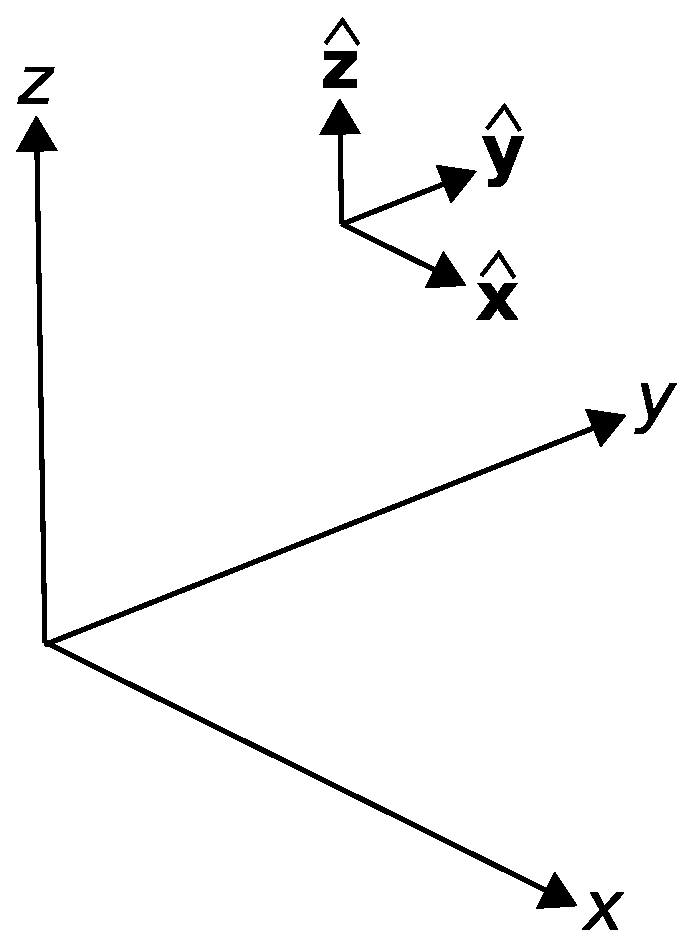
\includegraphics[width=1.5in]{modules/m0006_fCartesianBasis.eps}
% https://commons.wikimedia.org/wiki/File:M0006_fCartesianBasis.svg
}}{Shows the same Cartesian coordinate system from a previous figure. Overlayed on this is a smaller version of the coordinate system with the axes labeled x-hat, y-hat, and z-hat to correspond with the axis labels of the larger coordinate system.}
\end{center} 
\centerline{\scriptsize 
\copyright~\hyperref[m0006_fCartesianBasis_Credit]{K.\ Kikkeri} 
\href{https://creativecommons.org/licenses/by-sa/4.0/}{CC BY~SA 4.0} 
} 
\caption{
\label{m0006_fCartesianBasis}
Basis vectors in the Cartesian coordinate system.
}
\end{figure}

{\bf Vectors in the Cartesian Coordinate System.}
In Cartesian coordinates, we may describe any vector ${\bf A}$ as follows:
%
\begin{equation}
{\bf A} = \hat{\bf x}A_x + \hat{\bf y}A_y + \hat{\bf z}A_z
\end{equation} 
%
where $A_x$, $A_y$, and $A_z$ are scalar quantities describing the components of ${\bf A}$ in each of the associated directions, as shown in Figure~\ref{m0006_fVecCart}.
This description makes it clear that the magnitude of ${\bf A}$ is:
%
\begin{equation}
\left|{\bf A}\right| = \sqrt{ A_x^2 + A_y^2 + A_z^2 }
\end{equation}
%
and therefore, we can calculate the associated unit vector as
%
\begin{equation}
\begin{split}
\hat{\bf a} &= \frac{\bf A}{\left|{\bf A}\right|} = \frac{\bf A}{\sqrt{ A_x^2 + A_y^2 + A_z^2 }} \\
            &= ~~~\hat{\bf x}A_x \left( A_x^2 + A_y^2 + A_z^2 \right)^{-1/2} \\
            &~ ~~+\hat{\bf y}A_y \left( A_x^2 + A_y^2 + A_z^2 \right)^{-1/2} \\
            &~ ~~+\hat{\bf z}A_z \left( A_x^2 + A_y^2 + A_z^2 \right)^{-1/2} 
\end{split}
\end{equation}
%
\begin{figure}
\begin{center}
\pdftooltip{{  % note double braces
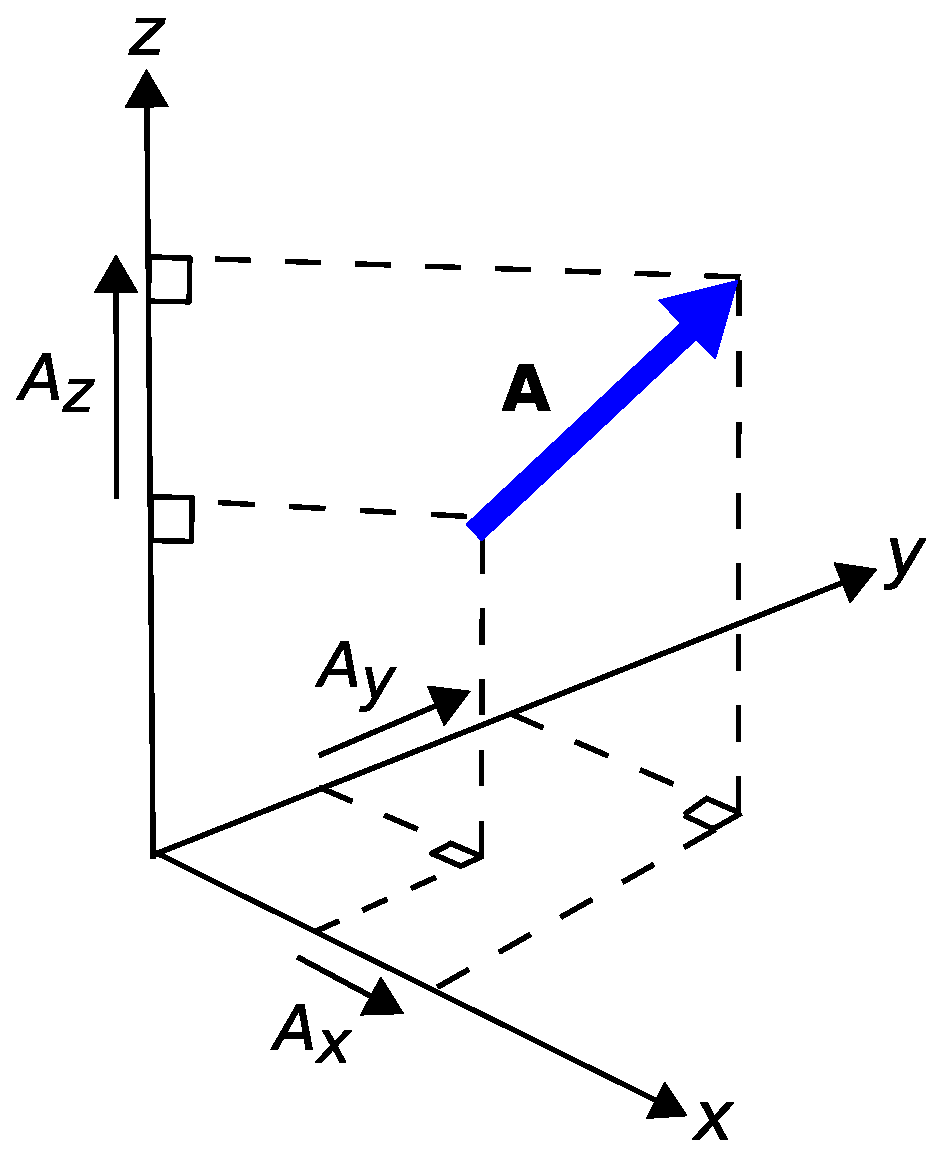
\includegraphics[width=2in]{modules/m0006_fVecCart.eps}
% https://commons.wikimedia.org/wiki/File:M0006_fVecCart.svg
}}{An arrow with a positive slope is arbitrarily positioned on the three dimensional Cartesian coordinate system. Dashed lines map the head and tail of the vector to each plane. The distances between the tale and head projection points on each axis are labeled A sub x, A sub y, and A sub z representing vector components.}
\end{center} 
\centerline{\scriptsize 
\copyright~\hyperref[m0006_fVecCart_Credit]{K.\ Kikkeri} 
\href{https://creativecommons.org/licenses/by-sa/4.0/}{CC BY~SA 4.0} 
} 
\caption{
\label{m0006_fVecCart}
Components of a vector ${\bf A}$ in the Cartesian coordinate system.
}
\end{figure}

{\bf Vector Addition and Subtraction.}
It is common to add and subtract vectors.
For example, vectors describing two forces ${\bf A}$ and ${\bf B}$ applied to the same point can be described as a single force vector ${\bf C}$ that is the sum of ${\bf A}$ and ${\bf B}$; i.e., ${\bf C}={\bf A}+{\bf B}$.
This addition is quite simple in the Cartesian coordinate system:
%
\begin{equation}
\begin{split}
{\bf C} &= {\bf A}+{\bf B} \\
        &= \left(\hat{\bf x}A_x + \hat{\bf y}A_y + \hat{\bf z}A_z\right) + \left( \hat{\bf x}B_x + \hat{\bf y}B_y + \hat{\bf z}B_z \right) \\
        &= \hat{\bf x}\left(A_x+B_x\right) + \hat{\bf y}\left(A_y+B_y\right) + \hat{\bf z}\left(A_z+B_z\right) 
\end{split}
\end{equation}
%
In other words, the $\hat{\bf x}$ component of ${\bf C}$ is the sum of the $\hat{\bf x}$ components of ${\bf A}$ and ${\bf B}$, and similarly for $\hat{\bf y}$ and $\hat{\bf z}$.
From the above example, it is clear that vector addition is commutative; i.e., 
%
\begin{equation}
{\bf A}+{\bf B} = {\bf B}+{\bf A}
\end{equation}
%
In other words, vectors may be added in any order.
Vector subtraction is defined similarly:
%
\begin{equation}
\begin{split}
{\bf D} &= {\bf A}-{\bf B} \\
        &= \left(\hat{\bf x}A_x + \hat{\bf y}A_y + \hat{\bf z}A_z\right) - \left( \hat{\bf x}B_x + \hat{\bf y}B_y + \hat{\bf z}B_z \right) \\
        &= \hat{\bf x}\left(A_x-B_x\right) + \hat{\bf y}\left(A_y-B_y\right) + \hat{\bf z}\left(A_z-B_z\right) 
\end{split}
\end{equation}
%
In other words, the $\hat{\bf x}$ component of ${\bf D}$ is the difference of the $\hat{\bf x}$ components of ${\bf A}$ and ${\bf B}$, and similarly for $\hat{\bf y}$ and $\hat{\bf z}$.
Like scalar subtraction, vector subtraction is \emph{not} commutative.

{\bf Relative Positions and Distances.}
A common task in vector analysis is to describe the position of one point in space relative to a different point in space. 
 Let us identify those two points using the position vectors ${\bf r}_1$ and ${\bf r}_2$, as indicated in Figure~\ref{m0006_fRelativePosition}. We may identify a third vector ${\bf r}_{12}$ as the position of ${\bf r}_{2}$ relative to ${\bf r}_{1}$:
%
\begin{equation}
{\bf r}_{12} \triangleq {\bf r}_{2} - {\bf r}_{1}
\end{equation}
%
Now $\left|{\bf r}_{12}\right|$ is the distance between these points, and ${\bf r}_{12}/\left|{\bf r}_{12}\right|$ is a unit vector indicating the direction to ${\bf r}_{2}$ from ${\bf r}_{1}$. 
%
\begin{figure}
\begin{center}
\pdftooltip{{  % note double brace
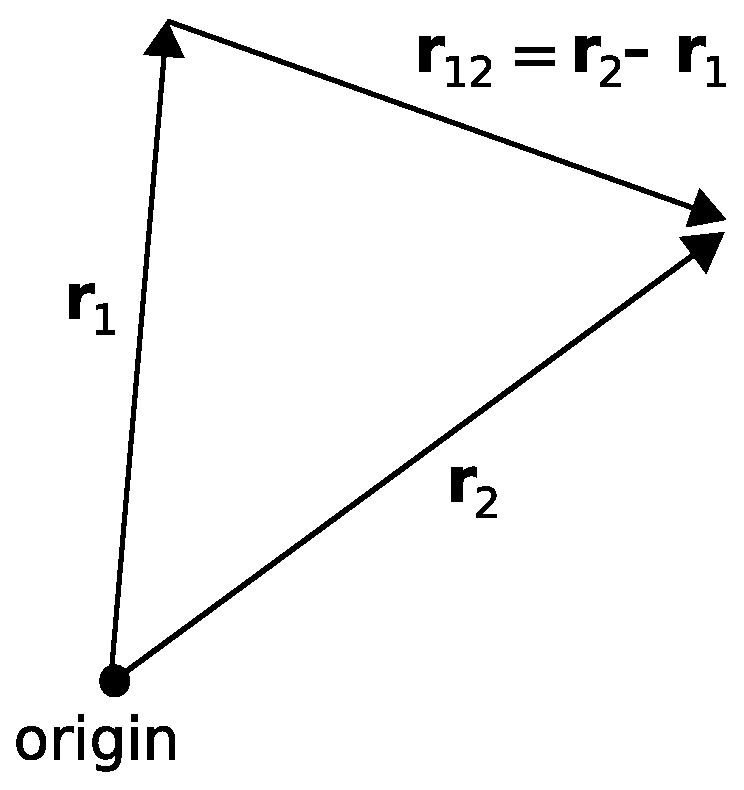
\includegraphics[width=1.5in]{modules/m0006_fRelativePosition.eps}
% https://commons.wikimedia.org/wiki/File:M0006_fRelativePosition.svg
}}{Two vectors of arbitrary lengths and direction, r sub 1 and r sub 2, emanate from the same point of origin. A third vector, r sub 12, starts at the head of r sub 1 and ends at the head of r sub 2. The third vector is labeled r sub 12 = r sub 2 - r sub 1.}
\end{center} 
\centerline{\scriptsize 
\copyright~\hyperref[m0006_fRelativePosition_Credit]{K.\ Kikkeri} 
\href{https://creativecommons.org/licenses/by-sa/4.0/}{CC BY~SA 4.0} 
} 
\caption{
\label{m0006_fRelativePosition}
Relative position (distance and direction) between locations identified by their position vectors.
}
\end{figure}

%%%%%%%%%%%%%%%%%%%%%%%%%%%%%%%%%%%%%%%%%%%%%%%%%%%%%%

%ORB EXAMPLE
~\\ \begin{example} 
\begin{mdframed}[backgroundcolor=brown!20,linecolor=brown!20]\raggedright
Direction and distance between positions.
\\~\\
Consider two positions, identified using the position vectors
${\bf r}_1 = 2\hat{\bf x} +3\hat{\bf y} +1\hat{\bf z}$ and
${\bf r}_2 = 1\hat{\bf x} -2\hat{\bf y} +3\hat{\bf z}$, both expressed in units of meters.
Find the direction vector that points from ${\bf r}_1$ to ${\bf r}_2$, the distance between these points, and the associated unit vector.

{\bf Solution.}
The vector that points from ${\bf r}_1$ to ${\bf r}_2$ is 
%
\begin{flalign}
{\bf R}  &= {\bf r}_2 - {\bf r}_1 \nonumber \\
         &= (1-2)\hat{\bf x} +(-2-3)\hat{\bf y} +(3-1)\hat{\bf z} \nonumber \\
         &= -\hat{\bf x} -5\hat{\bf y} +2\hat{\bf z} 
\end{flalign}
%
The distance between ${\bf r}_1$ and ${\bf r}_2$ is simply the magnitude of this vector:
%
\begin{equation}
\left|{\bf R}\right| = \sqrt{ \left(-1\right)^2  + \left(-5\right)^2  + \left(2\right)^2 } \cong 5.48~\mbox{m}
\end{equation}
%
The unit vector $\hat{\bf R}$ is simply ${\bf R}$ normalized to have unit magnitude:
%
\begin{flalign}
\hat{\bf R} &= {\bf R}/\left|{\bf R}\right| \nonumber \\
            &\cong \left(-\hat{\bf x} -5\hat{\bf y} +2\hat{\bf z}\right)/5.48 \nonumber \\
            &\cong -0.182\hat{\bf x} -0.913\hat{\bf y} +0.365\hat{\bf z}  
\end{flalign}

\end{mdframed}\end{example}


%---------------------------------------------------------------------------

{\bf Multiplication of a Vector by a Scalar.}
Let's say a particular force is specified by a vector ${\bf F}$.  What is the new vector if this force is doubled?  The answer is simply $2{\bf F}$ -- that is, twice the magnitude applied in the same direction.  This is an example of scalar multiplication of a vector.  Generalizing, the product of the scalar $\alpha$ and the vector ${\bf A}$ is simply $\alpha{\bf A}$.

\index{dot product|(}
\index{scalar product|see{dot product}}
{\bf Scalar (``Dot'') Product of Vectors.}
Another common task in vector analysis is to determine the similarity in the direction in which two vectors point.
In particular, it is useful to have a metric which, when applied to the vectors ${\bf A}=\hat{\bf a}A$ and ${\bf B}=\hat{\bf b}B$, has the following properties (see Figure~\ref{m0006_fDotProductSpecialCases}):
%
\begin{itemize}
\item If ${\bf A}$ is perpendicular to ${\bf B}$, the result is zero.
\item If ${\bf A}$ and ${\bf B}$ point in the same direction, the result is $AB$.
\item If ${\bf A}$ and ${\bf B}$ point in opposite directions, the result is $-AB$.
\item Results intermediate to these conditions depend on the angle $\psi$ between ${\bf A}$ and ${\bf B}$, measured as if ${\bf A}$ and ${\bf B}$ were arranged ``tail-to-tail'' as shown in Figure~\ref{m0006_fDotProduct}.
\end{itemize}
%
\begin{figure}
\begin{center}
\pdftooltip{{  % note double braces
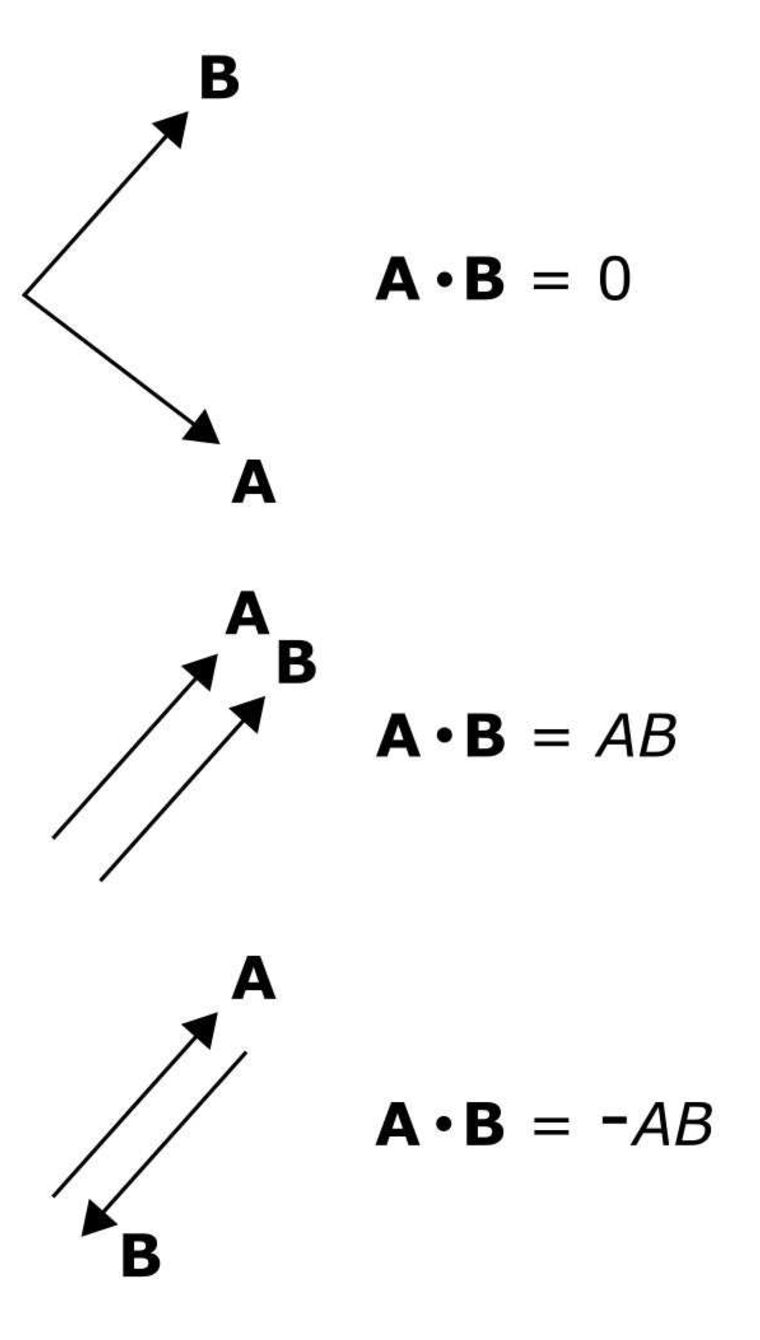
\includegraphics[width=1.5in]{modules/m0006_fDotProductSpecialCases.eps}
% https://commons.wikimedia.org/wiki/File:M0006_fDotProductSpecialCases.svg
}}{Three diagrams: top, middle, and bottom.
Top: Vectors A and B are perpendicular. vector A dot vector B = 0
Middle: Vectors A and B are parallel in the same direction. vector A dot vector B = AB
Bottom: Vectors A and B are parallel in opposite directions. vector A dot vector B = -AB
}
\end{center} 
\centerline{\scriptsize 
\copyright~\hyperref[m0006_fDotProductSpecialCases_Credit]{K.\ Kikkeri} 
\href{https://creativecommons.org/licenses/by-sa/4.0/}{CC BY~SA 4.0} 
} 
\caption{
\label{m0006_fDotProductSpecialCases}
Special cases of the dot product.
}
\end{figure}
%
In vector analysis, this operator is known as the \emph{scalar product} (not to be confused with scalar multiplication) or the \emph{dot product}.  
The dot product is written ${\bf A}\cdot{\bf B}$
and is given in general by the expression:
%
\begin{equation}
{\bf A}\cdot{\bf B} = AB\cos\psi
\label{m0006_eDPdef}
\end{equation}
%
Note that this expression yields the special cases previously identified, which are $\psi=\pi/2$, $\psi=0$, and $\psi=\pi$, respectively.
The dot product is commutative; i.e., 
%
\begin{equation}
{\bf A}\cdot{\bf B} = {\bf B}\cdot{\bf A} 
\end{equation}
%
The dot product is also distributive; i.e., 
%
\begin{equation}
{\bf A}\cdot\left({\bf B}+{\bf C}\right) = {\bf A}\cdot{\bf B}+{\bf A}\cdot{\bf C}
\end{equation}
%
\begin{figure}
\begin{center}
\pdftooltip{{  % note double braces
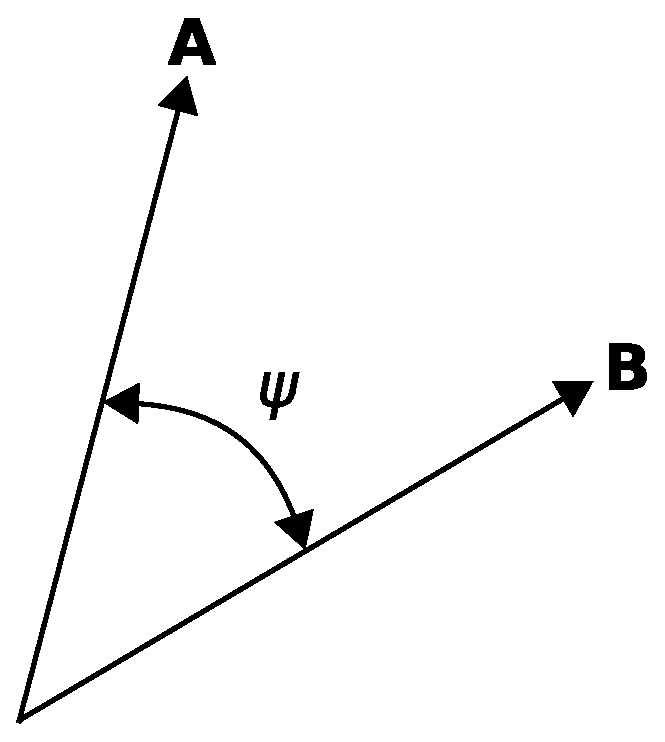
\includegraphics[width=1.5in]{modules/m0006_fDotProduct.eps}
% https://commons.wikimedia.org/wiki/File:M0006_fDotProduct.svg
}}{Vectors A and B emanate from the same point of origin to form an arbitrary acute angle. The angle between them is labeled psi.}
\end{center} 
\centerline{\scriptsize 
\copyright~\hyperref[m0006_fDotProduct_Credit]{K.\ Kikkeri} 
\href{https://creativecommons.org/licenses/by-sa/4.0/}{CC BY~SA 4.0} 
} 
\caption{
\label{m0006_fDotProduct}
Calculation of the dot product.
}
\end{figure}

The dot product has some other useful properties.
For example, note:
%
\begin{equation}
\begin{split}
{\bf A}\cdot{\bf A} &= \left(\hat{\bf x}A_x + \hat{\bf y}A_y + \hat{\bf z}A_z\right) \cdot \left(\hat{\bf x}A_x + \hat{\bf y}A_y + \hat{\bf z}A_z\right) \\
                    &= ~~\hat{\bf x}\cdot\hat{\bf x} A_x^2 + \hat{\bf x}\cdot\hat{\bf y} A_x A_y + \hat{\bf x}\cdot\hat{\bf z} A_x A_z \\
                    &~~  +\hat{\bf y}\cdot\hat{\bf x} A_x A_y + \hat{\bf y}\cdot\hat{\bf y} A_y^2 + \hat{\bf y}\cdot\hat{\bf z} A_y A_z \\
                    &~~  +\hat{\bf z}\cdot\hat{\bf x} A_x A_z + \hat{\bf z}\cdot\hat{\bf y} A_y A_z + \hat{\bf z}\cdot\hat{\bf z} A_z^2 
\end{split}
\end{equation}
%
which looks pretty bad until you realize that 
%
\begin{equation}
\hat{\bf x}\cdot\hat{\bf x} = \hat{\bf y}\cdot\hat{\bf y} = \hat{\bf z}\cdot\hat{\bf z} = 1
\end{equation}
%
and any other dot product of basis vectors is zero.  Thus, the whole mess simplifies to:
%
\begin{equation}
{\bf A}\cdot{\bf A} = A_x^2 + A_y^2 + A_z^2
\end{equation}
%
This is the square of the magnitude of ${\bf A}$, so we have discovered that
%
\begin{equation}
{\bf A}\cdot{\bf A} = \left|{\bf A}\right|^2 = A^2
\end{equation}
%
Applying the same principles to the dot product of potentially different vectors ${\bf A}$ and ${\bf B}$, we find:
%
\begin{equation}
\begin{split}
{\bf A}\cdot{\bf B} &= \left(\hat{\bf x}A_x + \hat{\bf y}A_y + \hat{\bf z}A_z\right) \cdot \left(\hat{\bf x}B_x + \hat{\bf y}B_y + \hat{\bf z}B_z\right) \\
                    &= A_x B_x + A_y B_y + A_z B_z
\end{split}
\label{m0006_eDPC}
\end{equation}
%
This is a particularly easy way to calculate the dot product, since it eliminates the problem of determining the angle $\psi$.
In fact, an easy way to calculate $\psi$ given ${\bf A}$ and ${\bf B}$ is to first calculate the dot product using Equation~\ref{m0006_eDPC} and then use the result to solve Equation~\ref{m0006_eDPdef} for $\psi$.

%ORB EXAMPLE
~\\ \begin{example} 
\begin{mdframed}[backgroundcolor=brown!20,linecolor=brown!20]\raggedright
Angle between two vectors. 
\\~\\
Consider the position vectors
${\bf C} = 2\hat{\bf x} +3\hat{\bf y} +1\hat{\bf z}$ and
${\bf D} = 3\hat{\bf x} -2\hat{\bf y} +2\hat{\bf z}$, both expressed in units of meters.
Find the angle between these vectors.

{\bf Solution.}
From Equation~\ref{m0006_eDPdef}
%
\begin{equation}
{\bf C}\cdot{\bf D} = CD\cos\psi
\end{equation}
%
where $C = \left|{\bf C}\right|$, $D = \left|{\bf D}\right|$, and $\psi$ is the angle we seek.
From Equation~\ref{m0006_eDPC}:
%
\begin{flalign}
{\bf C}\cdot{\bf D} &= C_x D_x + C_y D_y + C_z D_z \\
                    &= 2\cdot 3 + 3\cdot\left(-2\right) + 1\cdot 2 ~\mbox{m}^2 \\
                    &= 2 ~\mbox{m}^2
\end{flalign}
%
also
%
\begin{flalign}
C &= \sqrt{C_x^2 + C_y^2 + C_z^2} \cong 3.742~\mbox{m}  \\
D &= \sqrt{D_x^2 + D_y^2 + D_z^2} \cong 4.123~\mbox{m} 
\end{flalign}
so
%
\begin{equation}
\cos\psi = \frac{{\bf C}\cdot{\bf D}}{CD} \cong 0.130
\end{equation}
%
Taking the inverse cosine, we find $\psi=82.6^{\circ}$.

\end{mdframed}\end{example}
\index{dot product|)}

%-------------------------------------------------------------------------

\index{cross product|(}
{\bf Cross Product.}
The cross product is a form of vector multiplication that results in a vector that is perpendicular to both of the operands.
The definition is as follows:
%
\begin{equation}
{\bf A}\times{\bf B} = \hat{\bf n}AB\sin\psi_{AB}
\label{m0006_eCrossProduct}
\end{equation}
%
As shown in Figure~\ref{m0006_fCrossProduct}, the unit vector $\hat{\bf n}$ is determined by the ``right hand rule.'' 
\index{right-hand rule!cross product}
Using your right hand, curl your fingers to traverse the angle $\psi_{AB}$ beginning at ${\bf A}$ and ending at ${\bf B}$, and then $\hat{\bf n}$ points in the direction of your fully-extended thumb.  

It should be apparent that the cross product is not commutative but rather is \emph{anticommutative}; that is,
%
\begin{equation}
{\bf A}\times{\bf B} = -{\bf B}\times{\bf A} 
\end{equation}
%
You can confirm this for yourself using either Equation~\ref{m0006_eCrossProduct} or by applying the right-hand rule.

The cross product is distributive:
%
\begin{equation}
{\bf A}\times\left({\bf B} + {\bf C}\right) = {\bf A}\times{\bf B} + {\bf A}\times{\bf C} 
\end{equation}
%
\begin{figure}
\begin{center}
\pdftooltip{{  % note double braces
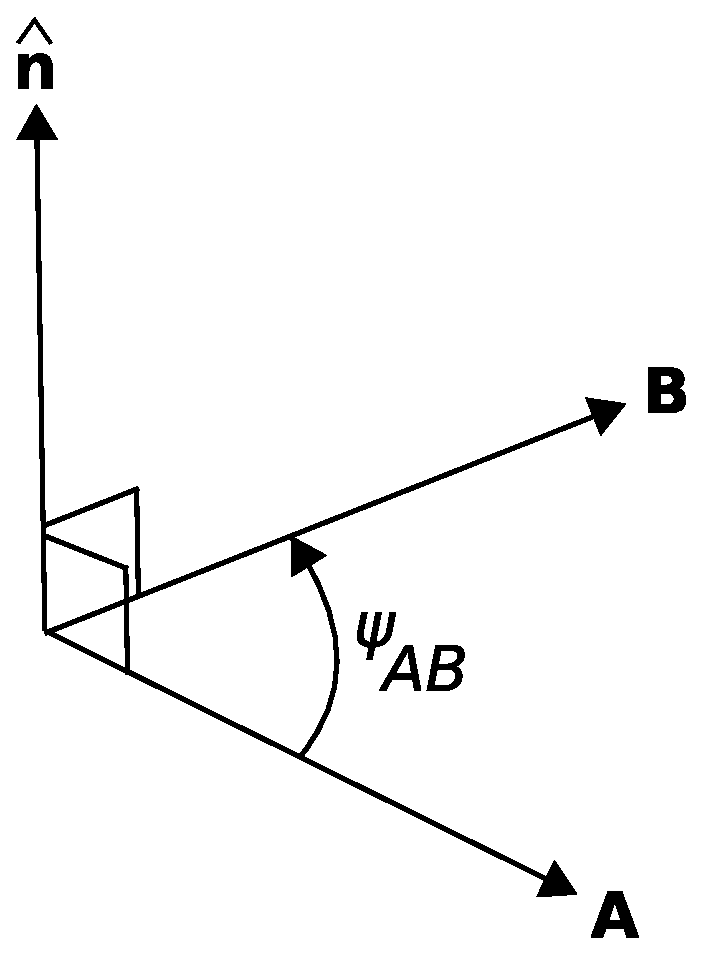
\includegraphics[width=1.5in]{modules/m0006_fCrossProduct.eps}
% https://commons.wikimedia.org/wiki/File:M0006_fCrossProduct.svg
}}{Three vectors are perpendicular to each other, labeled A, B, and n-hat. The angle formed by A and B is labeled psi sub AB}
\end{center} 
\centerline{\scriptsize 
\copyright~\hyperref[m0006_fCrossProduct_Credit]{K.\ Kikkeri} 
\href{https://creativecommons.org/licenses/by-sa/4.0/}{CC BY~SA 4.0} 
} 
\caption{
\label{m0006_fCrossProduct}
The cross product ${\bf A}\times{\bf B}$.
}
\end{figure}

There are two useful special cases of the cross product that are worth memorizing.  The first is the cross product of a vector with itself, which is zero:
%
\begin{equation}
{\bf A}\times{\bf A} = 0 
\end{equation}
%
The second is the cross product of vectors that are perpendicular; i.e., for which $\psi_{AB}=\pi/2$.  In this case:
%
\begin{equation}
{\bf A}\times{\bf B} = \hat{\bf n}AB 
\end{equation}
%
Using these principles, note:
%
\begin{equation}
\hat{\bf x} \times \hat{\bf x} = \hat{\bf y} \times \hat{\bf y} = \hat{\bf z} \times \hat{\bf z} = 0
\end{equation}
%
whereas
%
\begin{equation}
\hat{\bf x} \times \hat{\bf y} = \hat{\bf z}
\end{equation}
%
\begin{equation}
\hat{\bf y} \times \hat{\bf z} = \hat{\bf x}
\end{equation}
%
\begin{equation}
\hat{\bf z} \times \hat{\bf x} = \hat{\bf y}
\end{equation}
%
A useful diagram that summarizes these relationships is shown in Figure~\ref{m0006_fCartesianBasisCrossProducts}.
%
\begin{figure}
\begin{center}
\pdftooltip{{  % note double braces
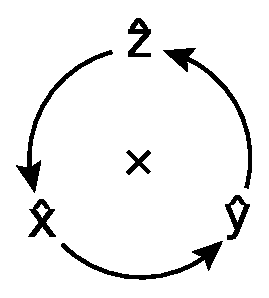
\includegraphics[width=1in]{modules/m0006_fCartesianBasisCrossProducts.eps}
}}{Arranged in a circle, x-hat, y-hat, and z-hat are arranged at 220, 300 and 90 degrees respectively. They are joined by semi-circular arrows pointing in the counter-clockwise direction. An x (cross) is at the center of the circle.}
\end{center} 
\caption{\label{m0006_fCartesianBasisCrossProducts}Cross products among basis vectors in the Cartesian system.  The cross product of any two basis vectors is the third basis vector when the order of operands is counter-clockwise, as shown in the diagram, and is $-1$ times the third basis vector when the order of operands is clockwise with respect to the arrangement in the diagram.}
\end{figure}

It is typically awkward to ``manually'' determine $\hat{\bf n}$ in Equation~\ref{m0006_eCrossProduct}.  
However, in Cartesian coordinates the cross product may be calculated as:
%
\begin{equation}
\begin{split}
{\bf A}\times{\bf B} =& ~~~~\hat{\bf x}\left(A_y B_z - A_z B_y \right) \\
                      & +\hat{\bf y}\left(A_z B_x - A_x B_z \right) \\
                      & +\hat{\bf z}\left(A_x B_y - A_y B_x \right) 
\end{split}
\end{equation}
%
This may be easier to remember as a matrix determinant:
%
\begin{equation}
{\bf A}\times{\bf B} =
\begin{vmatrix}
\hat{\bf x} & \hat{\bf y} & \hat{\bf z} \\
A_x & A_y & A_z \\
B_x & B_y & B_z 
\end{vmatrix}
\end{equation}
%
Similar expressions are available for other coordinate systems.

\index{cross product|)}

Vector analysis routinely requires expressions involving both dot products and cross products in different combinations.  Often, these expressions may be simplified, or otherwise made more convenient, using the vector identities listed in Appendix~\ref{m0140_Vector_Identities}.

%%%%%%%%%%%%%%%%%%%%%%%%%%%%%%%%%%%%

{\bf Additional Reading:}
\begin{itemize}
\item ``\href{https://en.wikipedia.org/wiki/Vector_field}{Vector field}'' on Wikipedia.
\item ``\href{https://en.wikipedia.org/wiki/Vector_algebra}{Vector algebra}'' on Wikipedia.
\end{itemize}

\index{vector!arithmetic|)}

      \vfill\break
    \section{Cartesian Coordinates}
{\color{blue}\tiny[m0004]}      % This is text associated with the open textbook "Open Electromagnetics"
% See immediately below for author, date
% This work is licensed under the Creative Commons Attribution-ShareAlike 4.0 International License. (CC BY-SA 4.0) 
% To view a copy of the license, visit http://creativecommons.org/licenses/by-sa/4.0/

%ORB TITLE Cartesian Coordinates
%ORB AUTHOR 0        # S.W. Ellingson, Virginia Tech (ellingson@vt.edu)
%ORB DATE 20180803   # yyyymmdd
%ORB ABSTRACT Cartesian Coordinates

\label{m0004_Cartesian_Coordinates} % <-- Must match name of this file and module directory name.  Don't mess with this!
\index{Cartesian coordinate system|(}

The Cartesian coordinate system is introduced in Section~\ref{m0006_Vector_Arithmetic}.
Concepts described in that section -- i.e., the dot product and cross product -- are described in terms of the Cartesian system.
In this section, we identify some additional features of this system that are useful in subsequent work and also set the stage for alternative systems; namely the cylindrical and spherical coordinate systems.  

{\bf Integration Over Length.}  
Consider a vector field ${\bf A}=\hat{\bf x}A({\bf r})$, where ${\bf r}$ is a position vector.
What is the integral of ${\bf A}$ over some curve $\mathcal{C}$ through space?
To answer this question, we first identify a differential-length segment of the curve. Note that this segment of the curve can be described as
%
\begin{equation}
d{\bf l} = \hat{\bf x}dx + \hat{\bf y}dy + \hat{\bf z}dz 
\end{equation}
%
The contribution to the integral for that segment of the curve is simply ${\bf A}\cdot d{\bf l}$. 
We integrate to obtain the result; i.e.,
%
\begin{equation}
\int_{\mathcal C}{ {\bf A}\cdot d{\bf l} }
\end{equation}
%
For example, 
%if ${\bf A}=\hat{\bf x}$ (i.e., $A({\bf r})=1$) 
if ${\bf A}=\hat{\bf x}A_0$ (i.e., $A({\bf r})$ is a constant) 
and if $\mathcal{C}$ is a straight line from $x=x_1$ and $x=x_2$ along some constant $y$ and $z$, then 
$d{\bf l} = \hat{\bf x}dx$, ${\bf A}\cdot d{\bf l}=A_0 dx$, and subsequently the above integral is
%
\begin{equation}
\int_{x_1}^{x_2}{ A_0 dx } = A_0\left(x_2-x_1\right)
\end{equation}
%
In particular, notice that if $A_0=1$, then this integral gives the length of ${\mathcal C}$.
Although the formalism seems unnecessary in this simple example, it becomes very useful when integrating over paths that vary in more than one direction and with more complicated integrands.

Note that the Cartesian system was an appropriate choice for preceding example because this allowed two of the three basis directions (i.e., $y$ and $z$) to be immediately eliminated from the calculation. %\footnote{If you care to look ahead, note that this is not possible in any other coordinate system.} 
Said differently, the preceding example is expressed with the minimum number of varying coordinates in the Cartesian system.
Here's a counter-example. If ${\mathcal C}$ had been a circle in the $z=0$ plane, then the problem would have required two basis directions to be considered -- namely, both $x$ and $y$. In this case, another system -- namely, cylindrical coordinates (Section~\ref{m0096_Cylindrical_Coordinates}) -- minimizes the number of varying coordinates (to just one, which is $\phi$).  

{\bf Integration Over Area.}  
Now we ask the question, what is the integral of some vector field ${\bf A}$ over some surface ${\mathcal S}$?
The answer is
%
\begin{equation}
\int_{\mathcal S}{{\bf A} \cdot d{\bf s}}
%\int_{x_1}^{x_2}\int_{y_1}^{y_2}{{\bf A} \cdot d{\bf s}}
\label{m0004_eFlux}
\end{equation} 
%
We refer to $d{\bf s}$ as the differential surface element, which is a vector having magnitude equal to the differential area $ds$, and is normal (perpendicular) to each point on the surface.
There are actually two such directions.  We'll return to clear up the ambiguity in a moment.
Now, as an example, if ${\bf A}=\hat{\bf z}$ and $\mathcal{S}$ is the surface bounded by $x_1\le x \le x_2$, $y_1\le y \le y_2$, then 
%
\begin{equation}
d{\bf s} = \hat{\bf z}~dx~dy
\end{equation}
%
since $dxdy$ is differential surface area in the $z=0$ plane and $\hat{\bf z}$ is normal to the $z=0$ plane.
So ${\bf A}\cdot d{\bf s}=dxdy$, and subsequently the integral in Equation~\ref{m0004_eFlux} becomes
%
\begin{equation}
\int_{x_1}^{x_2}\int_{y_1}^{y_2}{dx~dy} = \left(x_2-x_1\right)\left(y_2-y_1\right)
\end{equation} 
%
Note that this has turned out to be a calculation of area.

Once again, we see the Cartesian system was an appropriate choice for this example because this choice minimizes the number of varying coordinates; in the above example, the surface of integration is described by a constant value of $z$ with variable values of $x$ and $y$.
If the surface had instead been a cylinder or a sphere, not only would all three basis directions be variable, but also the surface normal would be variable, making the problem dramatically more complicated.  

Now let's return to the issue of the direction of $d{\bf s}$.  We chose $+\hat{\bf z}$, but why not choose $-\hat{\bf z}$ -- also a normal to the surface -- as this direction?  To answer simply, the resulting area would be negative.  ``Negative area'' is the expected (``positive'') area, except with respect to the opposite-facing normal vector.  In the present problem, the sign of the area is not important, but in some problems this sign becomes important.
One example of a class of problems for which the sign of area is important is when the quantity of interest is a \emph{flux}.  
\index{flux}
If ${\bf A}$ were a flux density, then the integration over area that we just performed indicates the magnitude \emph{and direction} of flux, and so the direction chosen for $d{\bf s}$ defines the direction of positive flux.  
Section~\ref{m0011_Electric_Flux_Density} describes the electric field in terms of a flux (i.e., as electric flux density ${\bf D}$), in which case positive flux flows away from a positively-charged source.

{\bf Integration Over Volume.}  
Another common task in vector analysis is integration of some quantity over a volume.
Since the procedure is the same for scalar or vector quantities, we shall consider integration of a scalar quantity $A({\bf r})$ for simplicity.
First, we note that the contribution from a differential volume element 
%
\begin{equation}
dv = dx~dy~dz
\end{equation}
%
is $A({\bf r})~dv$, so the integral over the volume ${\mathcal V}$ is
%
\begin{equation}
\int_{\mathcal V} A({\bf r})~dv
\end{equation}

For example, if $A({\bf r})=1$ and $\mathcal{V}$ is a cube bounded by $x_1\le x \le x_2$, $y_1\le y \le y_2$, and $z_1\le z \le z_2$, then the above integral becomes
%
\begin{equation}
\int_{x_1}^{x_2}\int_{y_1}^{y_2}\int_{z_1}^{z_2}{dx~dy~dz} = \left(x_2-x_1\right)\left(y_2-y_1\right)\left(z_2-z_1\right)
\end{equation} 
%
i.e., this is a calculation of volume.

The Cartesian system was an appropriate choice for this example because ${\mathcal V}$ is a cube, which is easy to describe in Cartesian coordinates and relatively difficult to describe in any other coordinate system.

%%%%%%%%%%%%%%%%%%%%%%%%%%%%%%%%%%%%

{\bf Additional Reading:}
\begin{itemize}
\item ``\href{https://en.wikipedia.org/wiki/Cartesian_coordinate_system}{Cartesian coordinate system}'' on Wikipedia.
\end{itemize}

\index{Cartesian coordinate system|)}

      \vfill\break
    \section{Cylindrical Coordinates}
{\color{blue}\tiny[m0096]}      % This is text associated with the open textbook "Open Electromagnetics"
% See immediately below for author, date
% This work is licensed under the Creative Commons Attribution-ShareAlike 4.0 International License. (CC BY-SA 4.0) 
% To view a copy of the license, visit http://creativecommons.org/licenses/by-sa/4.0/

%ORB TITLE Cylindrical Coordinates
%ORB AUTHOR 0        # S.W. Ellingson, Virginia Tech (ellingson@vt.edu)
%ORB DATE 20180803   # yyyymmdd
%ORB ABSTRACT Cylindrical Coordinates

\label{m0096_Cylindrical_Coordinates} % <-- Must match name of this file and module directory name.  Don't mess with this!
\index{cylindrical coordinate system|(}

Cartesian coordinates (Section~\ref{m0004_Cartesian_Coordinates}) are not convenient in certain cases.  
One of these is when the problem has cylindrical symmetry.
For example, in the Cartesian coordinate system, the cross-section of a cylinder concentric with the $z$-axis requires two coordinates to describe: $x$ and $y$.
However, this cross section can be described using a single parameter -- namely the radius -- which is $\rho$ in the cylindrical coordinate system.
This results in a dramatic simplification of the mathematics in some applications.

The cylindrical system is defined with respect to the Cartesian system in Figure~\ref{m0096_fCylindricalCoordinates}.
In lieu of $x$ and $y$, the cylindrical system uses $\rho$, the distance measured from the closest point on the $z$ axis,\footnote{Note that some textbooks use ``$r$'' in lieu of $\rho$ for this coordinate.} and $\phi$, the angle measured in a plane of constant $z$, beginning at the $+x$ axis ($\phi=0$) with $\phi$ increasing toward the $+y$ direction.
%
\begin{figure}[b!]
\begin{center}
\pdftooltip{{  % note double braces
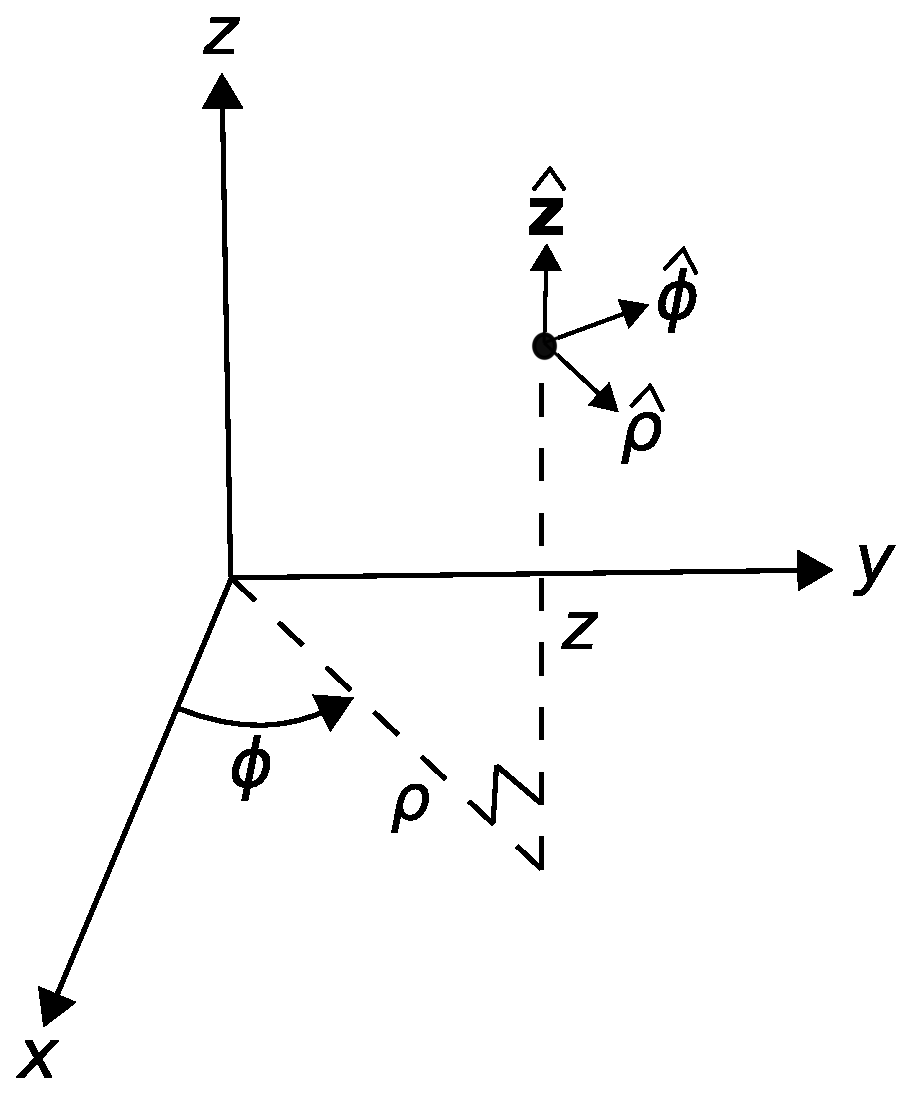
\includegraphics[width=2in]{modules/m0096_fCylindricalCoordinates.eps}
% https://commons.wikimedia.org/wiki/File:M0096_fCylindricalCoordinates.svg
}}{Cartesian coordinate system with a point arbitrarily plotted in the positive x, y, and z axes. A dashed line in the xy-plane labeled rho indicates the point’s distance from the z-axis and is shown at an angle phi from the x-axis. Another dashed line labeled z is perpendicular to rho, extends vertically from the xy-plane, and connects to the plotted point. The point has vector z-hat pointed in the z-direction. rho-hat points away from the origin, parallel to rho. phi-hat is perpendicular to z-hat and rho-hat.}
\end{center} 
\centerline{\scriptsize 
\copyright~\hyperref[m0096_fCylindricalCoordinates_Credit]{K.\ Kikkeri} 
\href{https://creativecommons.org/licenses/by-sa/4.0/}{CC BY~SA 4.0} 
} 
\caption{
\label{m0096_fCylindricalCoordinates}
Cylindrical coordinate system and associated basis vectors.
}
\end{figure}

The basis vectors in the cylindrical system are $\hat{\bf \rho}$, $\hat{\bf \phi}$, and $\hat{\bf z}$.
As in the Cartesian system, the dot product of like basis vectors is equal to one, and the dot product of unlike basis vectors is equal to zero.
The cross products of basis vectors are as follows:
%
\begin{equation}
\hat{\bf \rho} \times \hat{\bf \phi} = \hat{\bf z}
\end{equation}
%
\begin{equation}
\hat{\bf \phi} \times \hat{\bf z} = \hat{\bf \rho}
\end{equation}
%
\begin{equation}
\hat{\bf z} \times \hat{\bf \rho} = \hat{\bf \phi}
\end{equation}
%
A useful diagram that summarizes these relationships is shown in Figure~\ref{m0096_fCylindricalBasisCrossProducts}.
%
\begin{figure}
\begin{center}
\pdftooltip{{  % note double braces
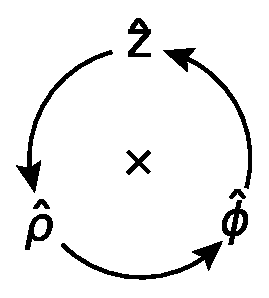
\includegraphics[width=1in]{modules/m0096_fCylindricalBasisCrossProducts.eps}
}}{The symbols for rho-hat, phi-hat, and z-hat are arranged in a circle, connected by arrows pointing in a counter-clockwise direction.  A cross product symbol appears in the center of the circle.}
\end{center} 
\caption{\label{m0096_fCylindricalBasisCrossProducts}Cross products among basis vectors in the cylindrical system. (See Figure~\ref{m0006_fCartesianBasisCrossProducts} for instructions on the use of this diagram.)}
\end{figure}

The cylindrical system is usually less useful than the Cartesian system for identifying absolute and relative positions.
This is because the basis directions depend on position.
For example, $\hat{\bf \rho}$ is directed radially outward from the $\hat{\bf z}$ axis, so $\hat{\bf \rho}=\hat{\bf x}$ for locations along the $x$-axis but $\hat{\bf \rho}=\hat{\bf y}$ for locations along the $y$ axis.
Similarly, the direction $\hat{\bf \phi}$ varies as a function of position.
To overcome this awkwardness, it is common to set up a problem in cylindrical coordinates in order to exploit cylindrical symmetry, but at some point to convert to Cartesian coordinates.  
Here are the conversions:
%
\begin{equation}
x = \rho\cos\phi
\end{equation}
%
\begin{equation}
y = \rho\sin\phi
\end{equation}
%
and $z$ is identical in both systems.  The conversion from Cartesian to cylindrical is as follows:
%
\begin{equation}
\rho = \sqrt{x^2+y^2}
\end{equation}
%
\begin{equation}
\phi = \arctan\left(y,x\right)
\end{equation}
%
where $\arctan$ is the \emph{four-quadrant} inverse tangent function; i.e., $\arctan(y/x)$ in the first quadrant ($x>0$, $y>0$), but possibly requiring an adjustment for the other quadrants because the signs of both $x$ and $y$ are individually significant.\footnote{Note that this function is available in MATLAB and Octave as {\tt atan2(y,x)}.}

Similarly, it is often necessary to represent basis vectors of the cylindrical system in terms of Cartesian basis vectors and vice-versa.
Conversion of basis vectors is straightforward using dot products to determine the components of the basis vectors in the new system. 
For example, $\hat{\bf x}$ in terms of the basis vectors of the cylindrical system is
%
\begin{equation}
\hat{\bf x} = \hat{\bf \rho}\left(\hat{\bf \rho}\cdot\hat{\bf x}\right) 
             +\hat{\bf \phi}\left(\hat{\bf \phi}\cdot\hat{\bf x}\right)
             +\hat{\bf z   }\left(\hat{\bf    z}\cdot\hat{\bf x}\right)
\end{equation}
%
The last term is of course zero since $\hat{\bf z}\cdot\hat{\bf x}=0$.
Calculation of the remaining terms requires dot products between basis vectors in the two systems, which are summarized in Table~\ref{m0096_tBasisVectorConversion}.
Using this table, we find
%
\begin{equation}
\hat{\bf x} = \hat{\bf \rho}\cos\phi
             -\hat{\bf \phi}\sin\phi
\end{equation}
%
\begin{equation}
\hat{\bf y} = \hat{\bf \rho}\sin\phi
             +\hat{\bf \phi}\cos\phi
\end{equation}
%
and of course $\hat{\bf z}$ requires no conversion.  Going from Cartesian to cylindrical, we find
%
\begin{equation}
\hat{\bf \rho} = \hat{\bf x}\cos\phi
                +\hat{\bf y}\sin\phi
\end{equation}
%
\begin{equation}
\hat{\bf \phi} =-\hat{\bf x}\sin\phi
                +\hat{\bf y}\cos\phi
\end{equation}
%
\begin{table}
\begin{center}
\begin{tabular}{c|ccc}
$\cdot$       & $\hat{\bf \rho}$ & $\hat{\bf \phi}$ & $\hat{\bf z}$ \\
\hline
$\hat{\bf x}$ & $\cos\phi$       & $-\sin\phi$      & 0 \\
$\hat{\bf y}$ & $\sin\phi$       & $~\cos\phi$      & 0 \\
$\hat{\bf z}$ & 0              & 0              & 1 \\
\end{tabular}
\end{center}
\caption{\label{m0096_tBasisVectorConversion}Dot products between basis vectors in the cylindrical and Cartesian coordinate systems.}
\end{table}

{\bf Integration Over Length.}  
A differential-length segment of a curve in the cylindrical system is described in general as
%
\begin{equation}
d{\bf l} = \hat{\bf \rho}d\rho + \hat{\bf \phi}\rho d\phi + \hat{\bf z}~dz 
\end{equation}
%
Note that the contribution of the $\phi$ coordinate to differential length is $\rho d\phi$, not simply $d\phi$.
This is because $\phi$ is an angle, not a distance. 
To see why the associated distance is $\rho d\phi$, consider the following.
The circumference of a circle of radius $\rho$ is $2\pi\rho$.  
If only a fraction of the circumference is traversed, the associated arclength is the circumference scaled by $\phi/2\pi$, where $\phi$ is the angle formed by the traversed circumference.
Therefore, the distance is $2\pi\rho \cdot \phi/2\pi = \rho \phi$, and the differential distance is $\rho d\phi$. 

As always, the integral of a vector field ${\bf A}({\bf r})$ over a curve ${\mathcal C}$ is
%
\begin{equation}
\int_{\mathcal C}{ {\bf A}\cdot d{\bf l} }
\end{equation}
%
To demonstrate the cylindrical system, let us calculate the integral of ${\bf A}({\bf r})=\hat{\bf \phi}$ when $\mathcal{C}$ is a circle of radius $\rho_0$ in the $z=0$ plane, as shown in Figure~\ref{m0096_Circle}.  In this example, 
$d{\bf l} = \hat{\bf \phi}~\rho_0~d\phi$ since $\rho=\rho_0$ and $z=0$ are both constant along ${\mathcal C}$.  Subsequently, ${\bf A}\cdot d{\bf l}=\rho_0 d\phi$ and the above integral is
%
\begin{equation}
\int_{0}^{2\pi}{ \rho_0~d\phi } = 2\pi\rho_0
\end{equation}
%
i.e., this is a calculation of circumference.
%
\begin{figure}
\begin{center}
\pdftooltip{{  % note double braces
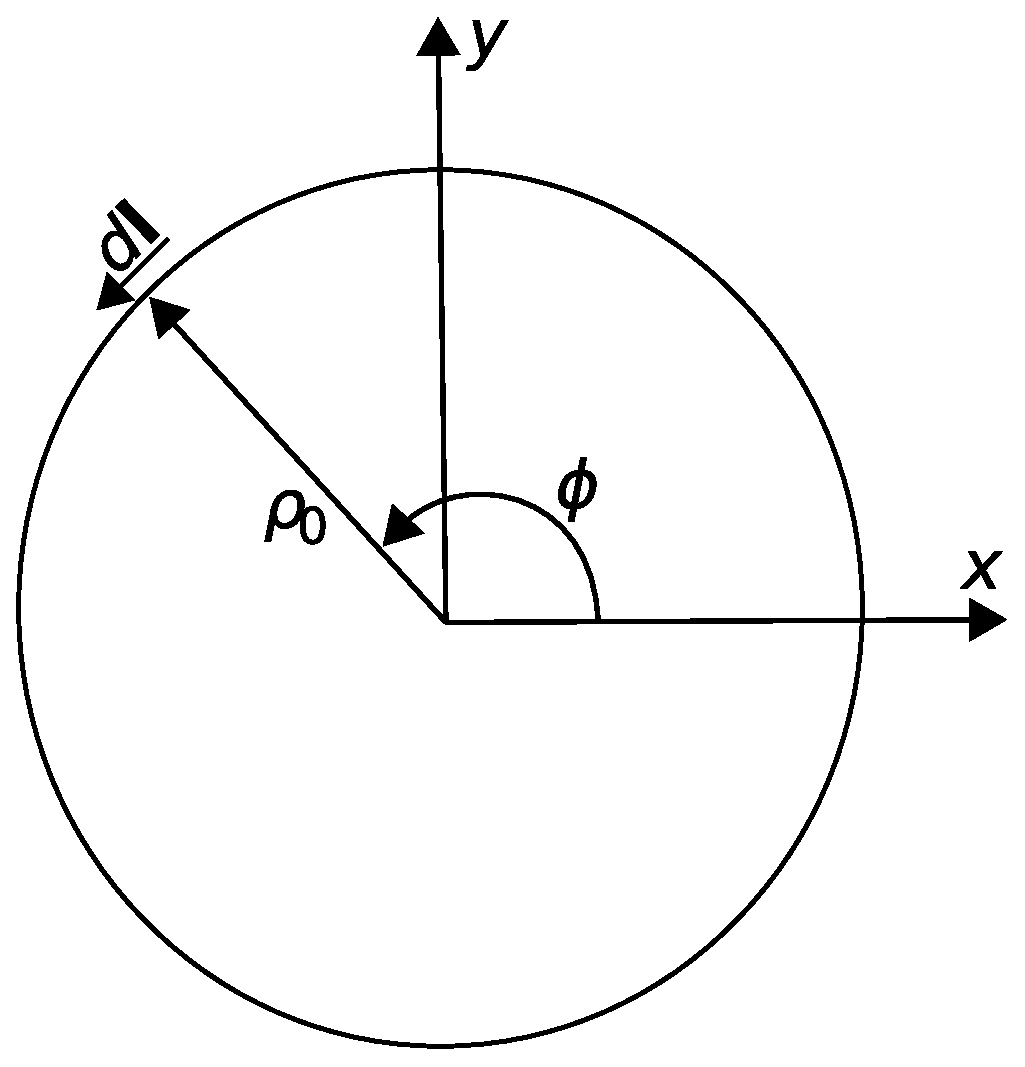
\includegraphics[width=2in]{modules/m0096_Circle.eps}
% https://commons.wikimedia.org/wiki/File:Cylindrical_Coordinates_Example.svg
}}{A circle lies in the traditional xy-plane with its center at the origin. Radius rho sub 0 is represented as a vector in the second quadrant of the coordinate system. phi represents the angle formed by the positive x-axis and rho sub 0. d vector l runs counterclockwise around the circumference of the circle.}
\end{center} 
\centerline{\scriptsize 
\copyright~\hyperref[m0096_Circle_Credit]{K.\ Kikkeri} 
\href{https://creativecommons.org/licenses/by-sa/4.0/}{CC BY~SA 4.0} 
} 
\caption{
\label{m0096_Circle}
Example in cylindrical coordinates: The circumference of a circle.
}
\end{figure}

Note that the cylindrical system is an appropriate choice for the preceding example because the problem can be expressed with the minimum number of varying coordinates in the cylindrical system.
If we had attempted this problem in the Cartesian system, we would find that both $x$ and $y$ vary over ${\mathcal C}$, and in a relatively complex way.\footnote{Nothing will drive this point home more firmly than trying it.  It can be done, but it's a lot more work...}

{\bf Integration Over Area.}  
Now we ask the question, what is the integral of some vector field ${\bf A}$ over a circular surface ${\mathcal S}$ in the $z=0$ plane having radius $\rho_0$? 
This is shown in Figure~\ref{m0096_CircleArea}.
The differential surface vector in this case is
%
\begin{equation}
d{\bf s} = \hat{\bf z}~\left( d\rho \right) \left( \rho d\phi \right) = \hat{\bf z}~\rho~d\rho~d\phi  
\end{equation}
%
The quantities in parentheses are the radial and angular dimensions, respectively.
The direction of $d{\bf s}$ indicates the direction of positive flux 
\index{flux}
-- see the discussion in Section~\ref{m0004_Cartesian_Coordinates} for an explanation.  
In general, the integral over a surface is
%
\begin{equation}
\int_{\mathcal S} {\bf A}\cdot d{\bf s}
\end{equation}
%
To demonstrate, let's consider ${\bf A}=\hat{\bf z}$; in this case ${\bf A}\cdot d{\bf s} = \rho~d\rho~d\phi$ and the integral becomes
%
\begin{equation}
\begin{split}
\int_{0}^{\rho_0}\int_{0}^{2\pi} \rho~d\rho~d\phi &= \left( \int_{0}^{\rho_0} \rho~d\rho \right) \left( \int_{0}^{2\pi} d\phi \right) \\
                                                  &= \left( \frac{1}{2}\rho_0^2 \right) \left( 2\pi \right) \\
                                                  &= \pi \rho_0^2
\end{split}
\end{equation}
%
which we recognize as the area of the circle, as expected.
The corresponding calculation in the Cartesian system is quite difficult in comparison.
%
\begin{figure}
\begin{center}
\pdftooltip{{  % note double braces
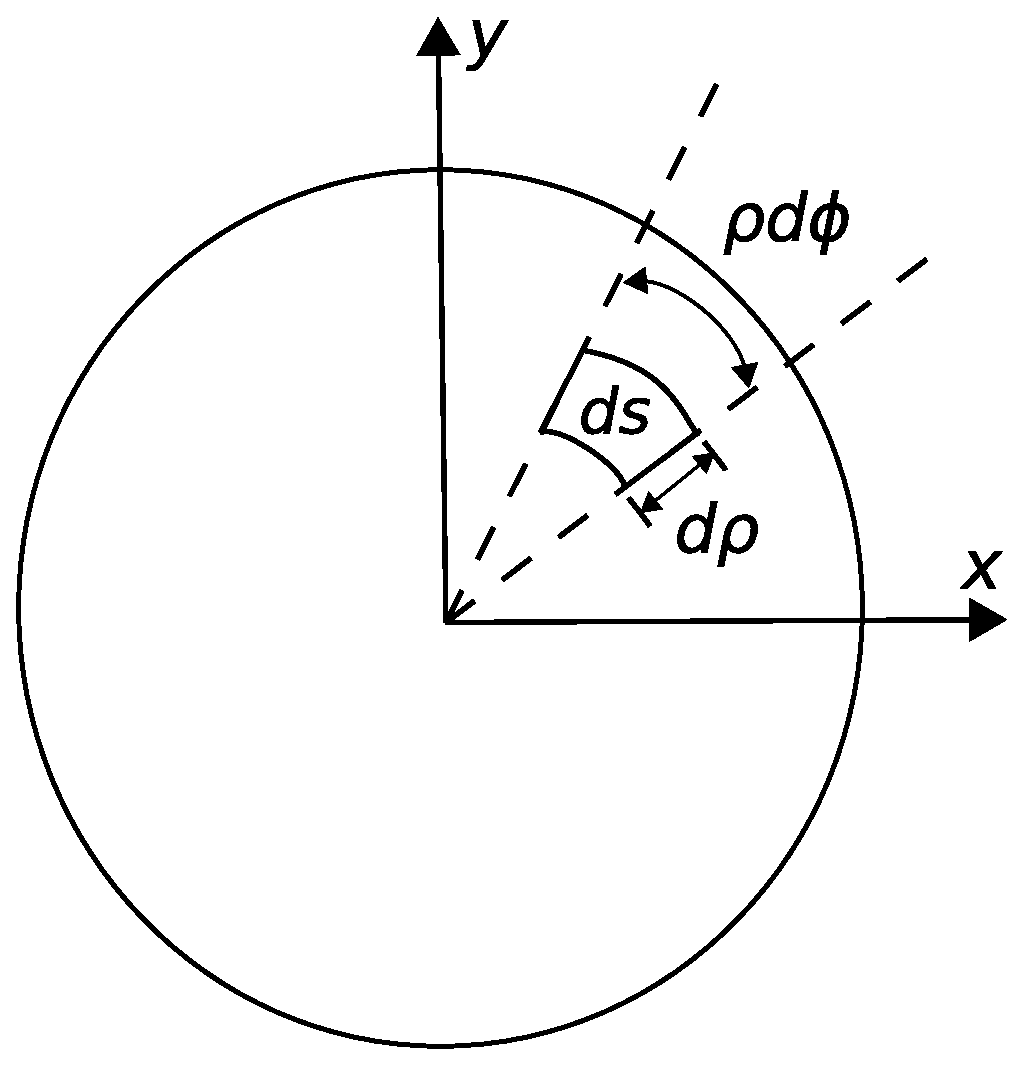
\includegraphics[width=2in]{modules/m0096_CircleArea.eps}
% https://commons.wikimedia.org/wiki/File:Cylindrical_Coordinates-Area_of_a_Circle.svg
}}{A circle in the xy-plane with its center at the origin. Two dashed lines emanate from the center of the circle to form an acute angle in the first quadrant of the circle. The section of the circumference blocked off by these two dashed lines is labeled rho * d phi. A section of the radius along one of the dashed lines is labeled d rho. This section of the radius is swept in the radial direction to the other dashed line to form a section of area called ds.}
\end{center} 
\centerline{\scriptsize 
\copyright~\hyperref[m0096_CircleArea_Credit]{K.\ Kikkeri} 
\href{https://creativecommons.org/licenses/by-sa/4.0/}{CC BY~SA 4.0} 
} 
\caption{
\label{m0096_CircleArea}
Example in cylindrical coordinates: The area of a circle.
}
\end{figure}

Whereas the previous example considered a planar surface, we might consider instead a curved surface.
Here we go.
What is the integral of a vector field ${\bf A}=\hat{\bf \rho}$ over a cylindrical surface ${\mathcal S}$ concentric with the $z$ axis having radius $\rho_0$ and extending from $z=z_1$ to $z=z_2$? 
This is shown in Figure~\ref{m0096_CylinderArea}.
%
\begin{figure}
\begin{center}
\pdftooltip{{  % note double braces
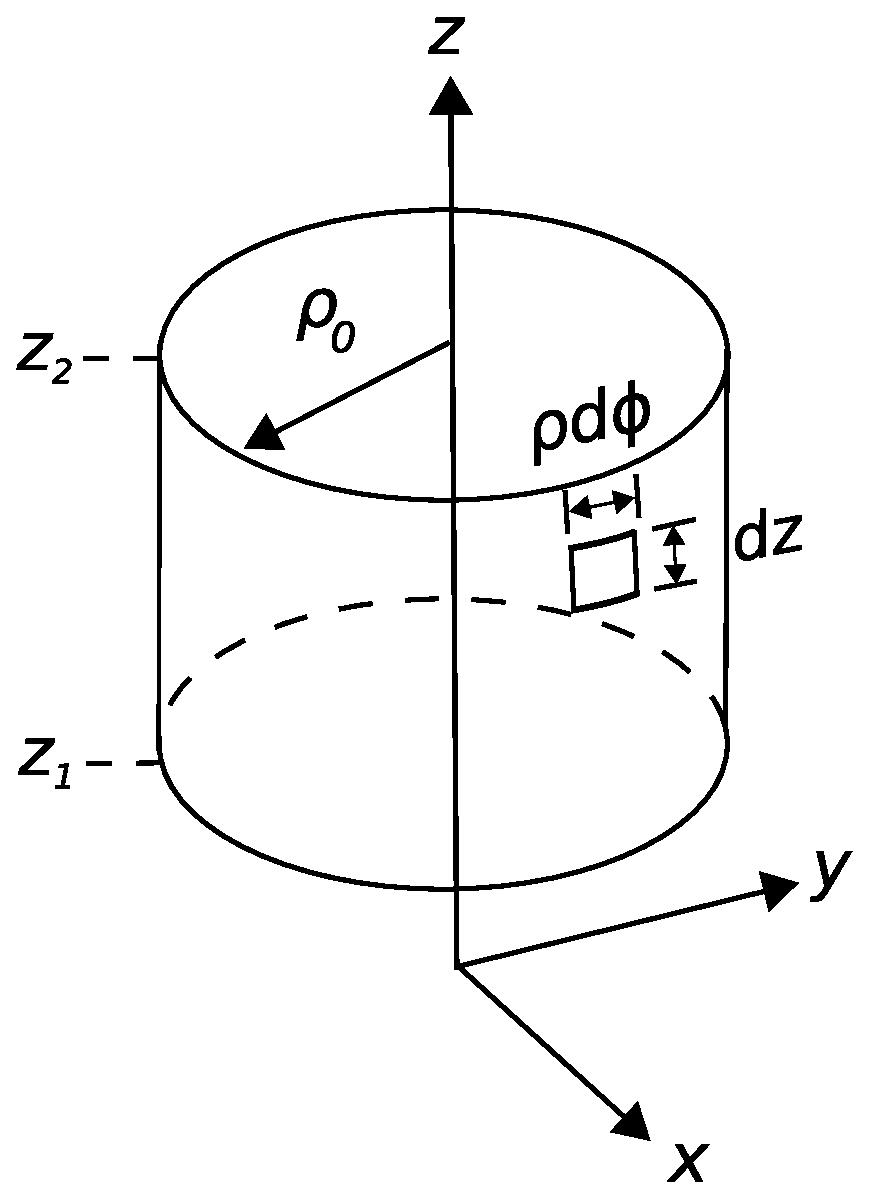
\includegraphics[width=2in]{modules/m0096_CylinderArea.eps}
% https://commons.wikimedia.org/wiki/File:M0096_CylinderArea.svg
}}{A cylinder lies in a Cartesian coordinate system with its centerline coincident with the positive z-axis. The height of the bottom surface of the cylinder is labeled z sub 1 and the height of the top surface is labeled z sub 2. The radius of the cylinder is labeled rho sub zero. An arbitrary section of the surface is described in width as rho d phi with height dz.}
\end{center} 
\centerline{\scriptsize 
\copyright~\hyperref[m0096_CylinderArea_Credit]{K.\ Kikkeri} 
\href{https://creativecommons.org/licenses/by-sa/4.0/}{CC BY~SA 4.0} 
} 
\caption{
\label{m0096_CylinderArea}
Example in cylindrical coordinates: The area of the curved surface of a cylinder.
}
\end{figure}
%
The differential surface vector in this case is
%
\begin{equation}
d{\bf s} = \hat{\bf \rho}\left( \rho_0 d\phi \right) \left( dz \right) = \hat{\bf \rho}\rho_0~d\phi~dz
\end{equation}
%
The integral is
%
\begin{equation}
\begin{split}
\int_{\mathcal S} {\bf A}\cdot d{\bf s} &= \int_{0}^{2\pi}\int_{z_1}^{z_2} \rho_0~d\phi dz \\
                                        &= \rho_0 \left( \int_{0}^{2\pi} d\phi \right) \left( \int_{z_1}^{z_2} dz \right)\\
                                        &= 2\pi \rho_0 \left(z_2-z_1\right) \\
\end{split}
\end{equation}
%
which is the area of ${\mathcal S}$, as expected.
Once again, the corresponding calculation in the Cartesian system is quite difficult in comparison.


{\bf Integration Over Volume.}  
The differential volume element in the cylindrical system is
%
\begin{equation}
dv ~=~ d\rho~\left(\rho d\phi\right)~dz ~=~ \rho~d\rho~d\phi~dz
\end{equation}

For example, if $A({\bf r})=1$ and the volume $\mathcal{V}$ is a cylinder bounded by $\rho\le \rho_0$ and $z_1\le z \le z_2$, then 
%
\begin{equation}
\begin{split}
\int_{\mathcal V} A({\bf r})~dv  &= \int_{0}^{\rho_0} \int_{0}^{2\pi} \int_{z_1}^{z_2} \rho~d\rho~d\phi~dz \\
                                 &= \left(\int_{0}^{\rho_0} \rho~d\rho \right)  \left( \int_{0}^{2\pi} d\phi \right)  \left( \int_{z_1}^{z_2} dz\right) \\
                                 & = \pi \rho_0^2 \left(z_2-z_1\right) 
\end{split}
\end{equation} 
%
i.e., area times length, which is volume.

Once again, the procedure above is clearly more complicated than is necessary if we are interested only in computing volume.
However, if the integrand is not constant-valued then we are no longer simply computing volume.
In this case, the formalism is appropriate and possibly necessary.  

%%%%%%%%%%%%%%%%%%%%%%%%%%%%%%%%%%%%

{\bf Additional Reading:}
\begin{itemize}
\item ``\href{https://en.wikipedia.org/wiki/Cylindrical_coordinate_system}{Cylindrical coordinate system}'' on Wikipedia.
\end{itemize}

\index{cylindrical coordinate system|)}

      \vfill\break
    \section{Spherical Coordinates}
{\color{blue}\tiny[m0097]}      % This is text associated with the open textbook "Open Electromagnetics"
% See immediately below for author, date
% This work is licensed under the Creative Commons Attribution-ShareAlike 4.0 International License. (CC BY-SA 4.0) 
% To view a copy of the license, visit http://creativecommons.org/licenses/by-sa/4.0/

%ORB TITLE Spherical Coordinates
%ORB AUTHOR 0        # S.W. Ellingson, Virginia Tech (ellingson@vt.edu)
%ORB DATE 20180703   # yyyymmdd
%ORB ABSTRACT Spherical Coordinates

\label{m0097_Spherical_Coordinates} % <-- Must match name of this file and module directory name.  Don't mess with this!
\index{spherical coordinate system|(}

The spherical coordinate system is defined with respect to the Cartesian system in Figure~\ref{m0097_fSphericalCoordinates}.
The spherical system uses $r$, the distance measured from the origin;\footnote{Note that some textbooks use ``$R$'' in lieu of $r$ for this coordinate.} $\theta$, the angle measured from the $+z$ axis toward the $z=0$ plane; and $\phi$, the angle measured in a plane of constant $z$, identical to $\phi$ in the cylindrical system.
%
\begin{figure}[b!]
\begin{center}
\pdftooltip{{  % note double braces
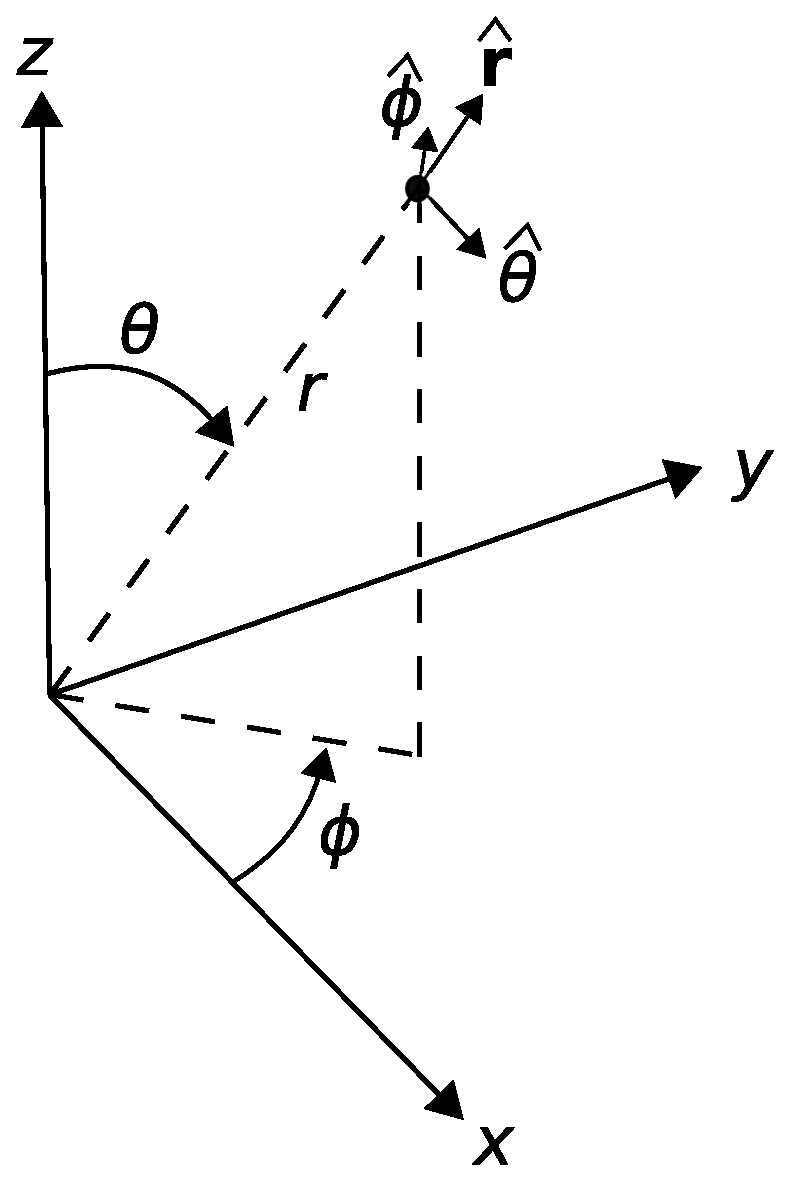
\includegraphics[width=2in]{modules/m0097_fSphericalCoordinates.eps}
% https://commons.wikimedia.org/wiki/File:Spherical_Coordinate_System.svg
}}{Cartesian coordinate system with a point arbitrarily plotted in the positive x, y, and z axes. A dashed line forms an acute triangle with one point at the origin of the Cartesian coordinate system and the top point connected to the arbitrary point with hypotenuse labeled r. The angle from the x-axis to the bottom side of the triangle is labeled phi. The angle from the z-axis to the hypotenuse is labeled theta. From the arbitrary point, vectors labeled phi-hat, r-hat, and theta-hat extend. The phi-hat vector extends parallel to the z-axis. Theta-hat extends parallel to the x-axis. R-hat is perpendicular to phi-hat and theta-hat.}
\end{center} 
\centerline{\scriptsize 
\copyright~\hyperref[m0097_fSphericalCoordinates_Credit]{K.\ Kikkeri} 
\href{https://creativecommons.org/licenses/by-sa/4.0/}{CC BY~SA 4.0} 
} 
\caption{
\label{m0097_fSphericalCoordinates}
Spherical coordinate system and associated basis vectors.
}
\end{figure}

Spherical coordinates are preferred over Cartesian and cylindrical coordinates when the geometry of the problem exhibits spherical symmetry.
For example, in the Cartesian coordinate system, the surface of a sphere concentric with the origin requires all three coordinates ($x$, $y$, and $z$) to describe.
However, this surface can be described using a single constant parameter -- the radius $r$ -- in the spherical coordinate system.
This leads to a dramatic simplification in the mathematics in certain applications.

The basis vectors in the spherical system are $\hat{\bf r}$, $\hat{\bf \theta}$, and $\hat{\bf \phi}$.
As always, the dot product of like basis vectors is equal to one, and the dot product of unlike basis vectors is equal to zero.
For the cross-products, we find:
%
\begin{equation}
\hat{\bf r} \times \hat{\bf \theta} = \hat{\bf \phi}
\end{equation}
%
\begin{equation}
\hat{\bf \theta} \times \hat{\bf \phi} = \hat{\bf r}
\end{equation}
%
\begin{equation}
\hat{\bf \phi} \times \hat{\bf r} = \hat{\bf \theta}
\end{equation}
%
A useful diagram that summarizes these relationships is shown in Figure~\ref{m0097_fSphericalBasisCrossProducts}.
%
\begin{figure}
\begin{center}
\pdftooltip{{  % note double braces
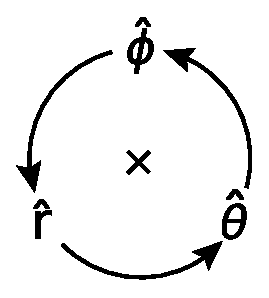
\includegraphics[width=1in]{modules/m0097_fSphericalBasisCrossProducts.eps}
}}{The symbols for r-hat, theta-hat, and phi-hat are arranged in a circle, connected by arrows pointing in a counter-clockwise direction.  A cross product symbol appears in the center of the circle.}
\end{center} 
\caption{\label{m0097_fSphericalBasisCrossProducts}Cross products among basis vectors in the spherical system. (See Figure~\ref{m0006_fCartesianBasisCrossProducts} for instructions on the use of this diagram.)}
\end{figure}

Like the cylindrical system, the spherical system is often less useful than the Cartesian system for identifying absolute and relative positions.
The reason is the same: Basis directions in the spherical system depend on position.
For example, $\hat{\bf r}$ is directed radially outward from the origin, so $\hat{\bf r}=\hat{\bf x}$ for locations along the $x$-axis but $\hat{\bf r}=\hat{\bf y}$ for locations along the $y$ axis and $\hat{\bf r}=\hat{\bf z}$ for locations along the $z$ axis.
Similarly, the directions of $\hat{\bf \theta}$ and $\hat{\bf \phi}$ vary as a function of position.
To overcome this awkwardness, it is common to begin a problem in spherical coordinates, and then to convert to Cartesian coordinates at some later point in the analysis.  
Here are the conversions:
%
\begin{align}
x &= r \cos\phi \sin\theta \label{m0097_es2cx} \\
y &= r \sin\phi \sin\theta \label{m0097_es2cy} \\
z &= r \cos\theta          \label{m0097_es2cz}
\end{align}
%
The conversion from Cartesian to spherical coordinates is as follows:
%
\begin{align}
r      &= \sqrt{x^2+y^2+z^2}      \\
\theta &= \arccos\left(z/r\right) \\
\phi   &= \arctan\left(y,x\right) \\
\end{align}
%
where $\arctan$ is the four-quadrant inverse tangent function.\footnote{Note that this function is available in MATLAB and Octave as {\tt atan2(y,x)}.}
%*** TODO PROBLEM *** \theta in terms of rho and z: 
%*** TODO PROBLEM *** cartesian to spherical conversion problem from page 7 of 3105 notes

Dot products between basis vectors in the spherical and Cartesian systems are summarized in Table~\ref{m0097_tBasisVectorConversion}.
This information can be used to convert between basis vectors in the spherical and Cartesian systems, in the same manner described in Section~\ref{m0096_Cylindrical_Coordinates}; e.g.
%
\begin{equation}
\hat{\bf x} = \hat{\bf r     }\left(\hat{\bf r     }\cdot\hat{\bf x}\right) 
             +\hat{\bf \theta}\left(\hat{\bf \theta}\cdot\hat{\bf x}\right)
             +\hat{\bf \phi  }\left(\hat{\bf \phi  }\cdot\hat{\bf x}\right)
\end{equation}
%
\begin{equation}
\hat{\bf r} = \hat{\bf x}\left(\hat{\bf x}\cdot\hat{\bf r}\right) 
             +\hat{\bf y}\left(\hat{\bf y}\cdot\hat{\bf r}\right)
             +\hat{\bf z}\left(\hat{\bf z}\cdot\hat{\bf r}\right)
\end{equation}
%
and so on.
%*** TODO PROBLEM *** write above explicitly
% 
%Using this table, we find
%%
%\begin{equation}
%\hat{\bf x} = \hat{\bf r}\sin\theta\cos\phi
%             +\hat{\bf \theta}\cos\theta\cos\phi
%             -\hat{\bf \phi}\sin\phi
%%\end{equation}
%%
%\begin{equation}
%\hat{\bf y} = \hat{\bf r}\sin\theta\sin\phi
%             +\hat{\bf \theta}\cos\theta\sin\phi
%             +\hat{\bf \phi}\cos\phi
%\end{equation}
%%
%\begin{equation}
%\hat{\bf z} = \hat{\bf r}\cos\theta
%             -\hat{\bf \theta}\sin\theta
%\end{equation}
%
\begin{table}
\begin{center}
\begin{tabular}{c|ccc}
$\cdot$       & $\hat{\bf r}$ & $\hat{\bf \theta}$ & $\hat{\bf \phi}$ \\
\hline
$\hat{\bf x}$ & $\sin\theta\cos\phi$ & $~\cos\theta\cos\phi$ & $-\sin\phi$ \\
$\hat{\bf y}$ & $\sin\theta\sin\phi$ & $~\cos\theta\sin\phi$ & $~\cos\phi$ \\
$\hat{\bf z}$ & $\cos\theta$         & $-\sin\theta$         & 0 \\
\end{tabular}
\end{center}
\caption{\label{m0097_tBasisVectorConversion}Dot products between basis vectors in the spherical and Cartesian coordinate systems.}
\end{table}

%ORB EXAMPLE
~\\ \begin{example} 
\begin{mdframed}[backgroundcolor=brown!20,linecolor=brown!20]\raggedright
Cartesian to spherical conversion. 
\\~\\
A vector field ${\bf G} = \hat{\bf x}~xz/y$.  Develop an expression for ${\bf G}$ in spherical coordinates.

{\bf Solution:} Simply substitute expressions in terms of spherical coordinates for expressions in terms of Cartesian coordinates. 
Use Table~\ref{m0097_tBasisVectorConversion} and Equations~\ref{m0097_es2cx}--\ref{m0097_es2cz}. 
Making these substitutions and applying a bit of mathematical clean-up afterward, one obtains  
%
\begin{align}
{\bf G} =& \left( \hat{\bf r}\sin\theta\cot\phi + \hat{\bf\phi}\cos\theta\cot\phi - \hat{\bf \phi} \right) \nonumber \\
         & \cdot r\cos\theta\cos\phi
\end{align}

\end{mdframed}\end{example}


%---------------------------------------------------------------------

{\bf Integration Over Length.}  
A differential-length segment of a curve in the spherical system is
%
\begin{equation}
d{\bf l} = \hat{\bf r}~dr + \hat{\bf \theta}~r~d\theta + \hat{\bf \phi}~r\sin\theta~d\phi 
\end{equation}
%
Note that $\theta$ is an angle, as opposed to a distance. The associated distance is $r~d\theta$ in the $\theta$ direction.
Note also that in the $\phi$ direction, distance is $r~d\phi$ in the $z=0$ plane and less by the factor $\sin\theta$ for $z<>0$. 

As always, the integral of a vector field ${\bf A}({\bf r})$ over a curve ${\mathcal C}$ is
%
\begin{equation}
\int_{\mathcal C}{ {\bf A}\cdot d{\bf l} }
\end{equation}
%
To demonstrate line integration in the spherical system, imagine a sphere of radius $a$ centered at the origin with ``poles'' at $z=+a$ and $z=-a$.
Let us calculate the integral of ${\bf A}({\bf r})=\hat{\bf \theta}$, where $\mathcal{C}$ is the arc drawn directly from pole to pole along the surface of the sphere, as shown in Figure~\ref{m0097_fArc}.  In this example, 
$d{\bf l} = \hat{\bf \theta}~a~d\theta$ 
since $r=a$ and $\phi$ (which could be any value) are both constant along ${\mathcal C}$.  
Subsequently, ${\bf A}\cdot d{\bf l}=a~d\theta$ and the above integral is
%
\begin{equation}
\int_{0}^{\pi}{ a~d\theta } = \pi a
\end{equation}
%
i.e., half the circumference of the sphere, as expected.
%
\begin{figure}
\begin{center}
\pdftooltip{{  % note double braces
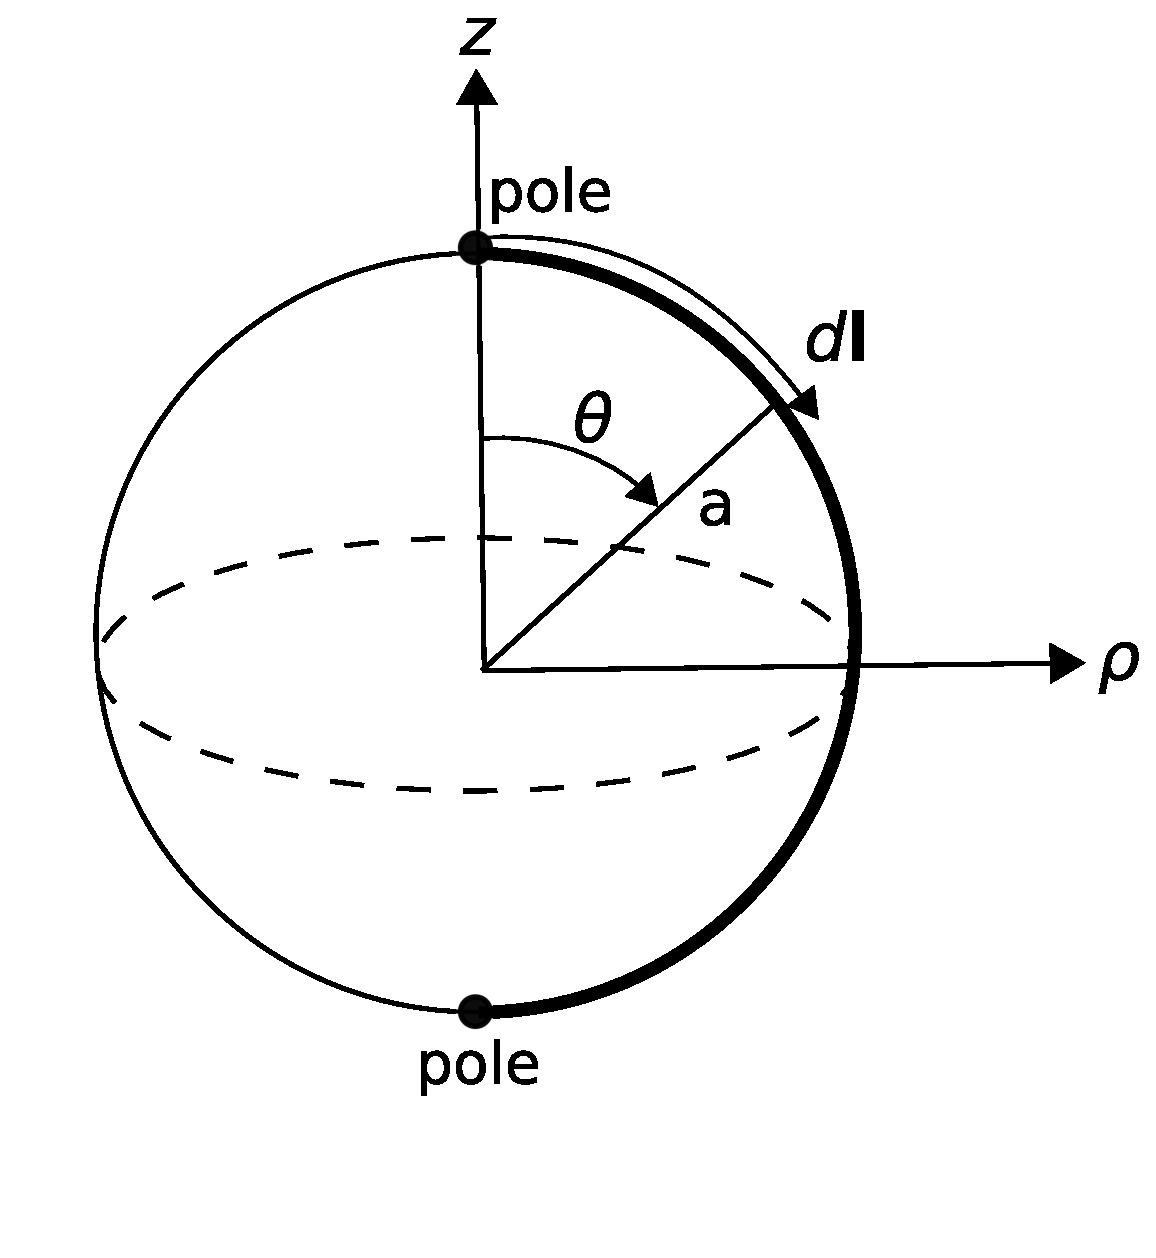
\includegraphics[width=2in]{modules/m0097_fArc.eps}
% https://commons.wikimedia.org/wiki/File:M0097_fArc.svg
}}{A three dimensional sphere centered at the intersection of the rho and z axes. The radius (a) shown at unspecified angle in the first quadrant of the sphere. The north and south poles of the sphere are labeled, and the circumference between them is bolded. From the north pole to the radius (a) is a vector labeled dl. The angle from the z-axis to the radius (a) is labeled theta. }
\end{center} 
\centerline{\scriptsize 
\copyright~\hyperref[m0097_fArc_Credit]{K.\ Kikkeri} 
\href{https://creativecommons.org/licenses/by-sa/4.0/}{CC BY~SA 4.0} 
} 
\caption{
\label{m0097_fArc}
Example in spherical coordinates: Pole-to-pole distance on a sphere.
}
\end{figure}

Note that the spherical system is an appropriate choice for this example because the problem can be expressed with the minimum number of varying coordinates in the spherical system.
If we had attempted this problem in the Cartesian system, we would find that both $z$ and either $x$ or $y$ (or all three) vary over ${\mathcal C}$ and in a relatively complex way. 

{\bf Integration Over Area.}  
Now we ask the question,
what is the integral of some vector field ${\bf A}$ over the surface ${\mathcal S}$ of a sphere of radius $a$ centered on the origin?
This is shown in Figure~\ref{m0097_fSphereArea}.
The differential surface vector in this case is
%
\begin{equation}
d{\bf s} = \hat{\bf r}~\left( r~d\theta \right) \left( r\sin\theta~d\phi \right) = \hat{\bf r}~r^2\sin\theta~d\theta~d\phi  
\end{equation}
%
As always, the direction is normal to the surface and in the direction associated with positive flux.
\index{flux}
The quantities in parentheses are the distances associated with varying $\theta$ and $\phi$, respectively.
In general, the integral over a surface is
%
\begin{equation}
\int_{\mathcal S} {\bf A}\cdot d{\bf s}
\end{equation}
%
In this case, let's consider ${\bf A}=\hat{\bf r}$; in this case ${\bf A}\cdot d{\bf s} = a^2~\sin\theta~d\theta~d\phi$ and the integral becomes
%
\begin{equation}
\begin{split}
\int_{0}^{\pi}\int_{0}^{2\pi} a^2~\sin\theta~d\theta~d\phi &= a^2 \left( \int_{0}^{\pi} \sin\theta d\theta \right) \left( \int_{0}^{2\pi} d\phi \right) \\
                                                           &= a^2 \left( 2 \right) \left( 2\pi \right) \\
                                                           &= 4\pi a^2
\end{split}
\end{equation}
%
which we recognize as the area of the sphere, as expected.
The corresponding calculation in the Cartesian or cylindrical systems is quite difficult in comparison.
%
\begin{figure}
\begin{center}
\pdftooltip{{  % note double braces
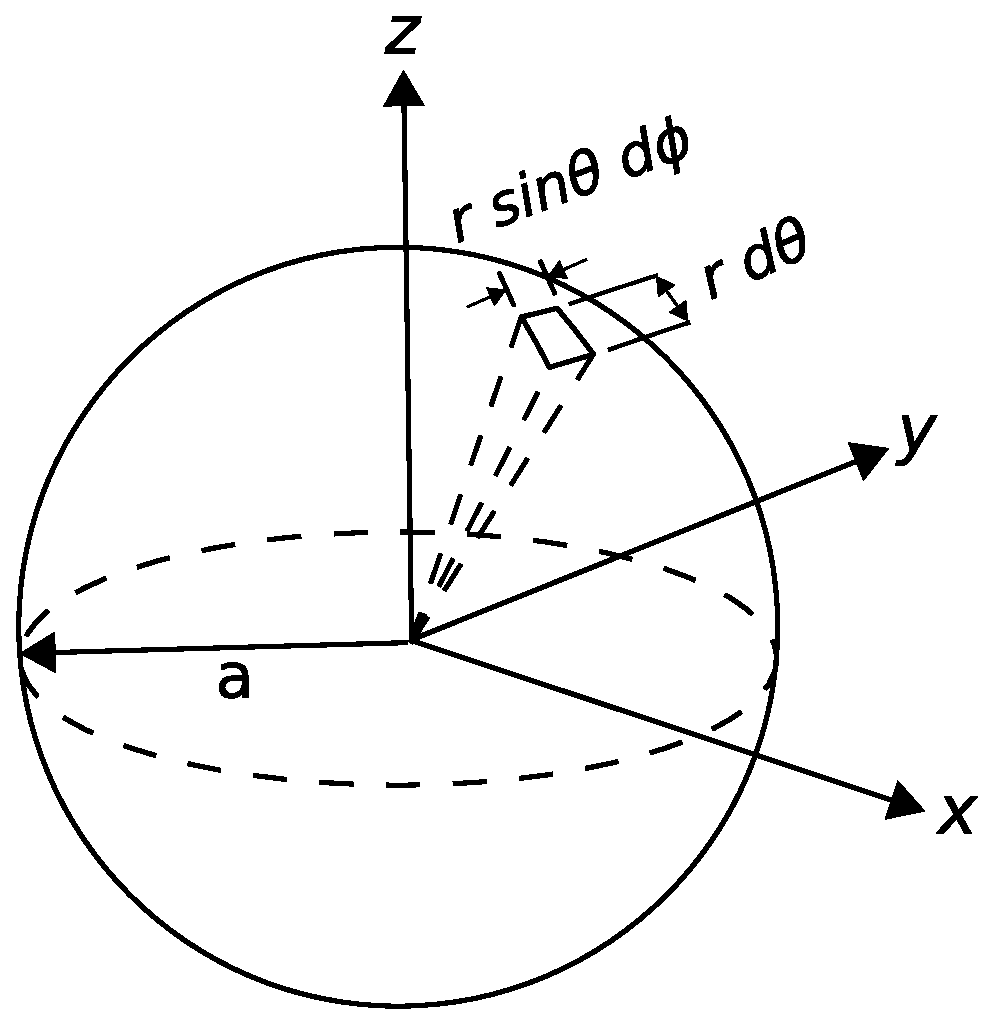
\includegraphics[width=2in]{modules/m0097_fSphereArea.eps}
% https://commons.wikimedia.org/wiki/File:M0097_fSphereArea.svg
}}{A three dimensional sphere lies on a x, y, z axis, with its center at the origin. The radius is labeled a. A square is projected on the surface from the origin, with dashed lines indicating the projection. The width of the box is labeled r * sin(theta) * d phi, and the height of the box is labeled r * d theta.}
\end{center} 
\centerline{\scriptsize 
\copyright~\hyperref[m0097_fSphereArea_Credit]{K.\ Kikkeri} 
\href{https://creativecommons.org/licenses/by-sa/4.0/}{CC BY~SA 4.0} 
} 
\caption{
\label{m0097_fSphereArea}
Example in spherical coordinates: The area of a sphere.
}
\end{figure}

%%% TODO
%~\\ \begin{example} 
%\begin{mdframed}[backgroundcolor=green!20] 
%Flux Through a Spherical Surface. 
%\end{mdframed}
%{\color{red}uniform flux in cartesian direction gives zero flux through sphere but non-zero flux through a half-sphere.}
%\centerline{\rule{2in}{1pt}} \end{example}


%---------------------------------------------------------------------

{\bf Integration Over Volume.}  
The differential volume element in the spherical system is
%
\begin{equation}
dv ~=~ dr \left(r d\theta \right) \left( r \sin\theta d\phi \right) ~=~ r^2 dr~\sin\theta~d\theta~d\phi 
\end{equation}

For example, if $A({\bf r})=1$ and the volume $\mathcal{V}$ is a sphere of radius $a$ centered on the origin, then 
%
\begin{equation}
\begin{split}
\int_{\mathcal V} A({\bf r})~dv  &= \int_0^a \int_0^{\pi} \int_0^{2\pi}  r^2 dr~\sin\theta~d\theta~d\phi \\
                                 &= \left(\int_0^a r^2 dr \right)  \left( \int_0^{\pi} \sin\theta~d\theta \right)  \left( \int_0^{2\pi} d\phi \right) \\
                                 &= \left( \frac{1}{3} a^3 \right)  \left( 2 \right)  \left(  2\pi \right) \\
                                 &= \frac{4}{3}\pi a^3 
\end{split}
\end{equation} 
%
which is the volume of a sphere. 

%%%%%%%%%%%%%%%%%%%%%%%%%%%%%%%%%%%%

{\bf Additional Reading:}
\begin{itemize}
\item ``\href{https://en.wikipedia.org/wiki/Spherical_coordinate_system}{Spherical coordinate system}'' on Wikipedia.
\end{itemize}

\index{spherical coordinate system|)}

      \vfill\break
    \section{Gradient}
{\color{blue}\tiny[m0098]}      % This is text associated with the open textbook "Open Electromagnetics"
% See immediately below for author, date
% This work is licensed under the Creative Commons Attribution-ShareAlike 4.0 International License. (CC BY-SA 4.0) 
% To view a copy of the license, visit http://creativecommons.org/licenses/by-sa/4.0/

%ORB TITLE Gradient
%ORB AUTHOR 0        # S.W. Ellingson, Virginia Tech (ellingson@vt.edu)
%ORB DATE 20180803   # yyyymmdd
%ORB ABSTRACT Gradient 

\label{m0098_Gradient} % <-- Must match name of this file and module directory name.  Don't mess with this!
\index{gradient|(}

The gradient operator is an important and useful tool in electromagnetic theory.
Here's the main idea:
%
%ORB HIGHLIGHT
\begin{mdframed}[backgroundcolor=yellow!20,nobreak=true] 
The \emph{gradient} of a scalar field is a vector that points in the direction in which the field is most rapidly increasing, with the scalar part equal to the rate of change.
\end{mdframed}

A particularly important application of the gradient is that it relates the electric field intensity ${\bf E}({\bf r})$ to the electric potential field $V({\bf r})$.
This is apparent from a review of Section~\ref{m0002_Electric_Field_Intensity} (``Electric Field Intensity''); see in particular, the battery-charged capacitor example.
In that example, it is demonstrated that:
%
\begin{itemize} 
\item The \emph{direction} of ${\bf E}({\bf r})$ is the direction in which $V({\bf r})$ decreases most quickly, and
\item The \emph{scalar part} of ${\bf E}({\bf r})$ is the rate of change of $V({\bf r})$ in that direction. Note that this is also implied by the units, since $V({\bf r})$ has units of V whereas ${\bf E}({\bf r})$ has units of V/m.
\end{itemize}
%
The gradient is the mathematical operation that relates the vector field ${\bf E}({\bf r})$ to the scalar field $V({\bf r})$ and is indicated by the symbol ``$\nabla$'' as follows:
%
\begin{equation}
{\bf E}({\bf r}) = -\nabla V({\bf r})
\end{equation}
%
or, with the understanding that we are interested in the gradient as a function of position ${\bf r}$, simply
%
\begin{equation}
{\bf E} = -\nabla V
\end{equation}

At this point we should note that the gradient is a very general concept, and that we have merely identified one application of the gradient above.  In electromagnetics there are many situations in which we seek the gradient $\nabla f$ of some scalar field $f({\bf r})$.  Furthermore, we find that other differential operators that are important in electromagnetics can be interpreted in terms of the gradient operator $\nabla$.  These include
\emph{divergence} (Section~\ref{m0044_Divergence}), 
\emph{curl} (Section~\ref{m0048_Curl}), 
and the \emph{Laplacian} (Section~\ref{m0099_The_Laplacian_Operator}).

In the Cartesian system:
%
\begin{equation}
\nabla f = \hat{\bf x}\frac{\partial f}{\partial x} + \hat{\bf y}\frac{\partial f}{\partial y} + \hat{\bf z}\frac{\partial f}{\partial z} 
\label{eDelCar}
\end{equation}

%ORB EXAMPLE
~\\ \begin{example} 
\begin{mdframed}[backgroundcolor=brown!20,linecolor=brown!20]\raggedright
Gradient of a ramp function.
\\~\\
Find the gradient of $f=ax$ (a ``ramp'' having slope $a$ along the $x$ direction).

{\bf Solution.} 
Here, $\partial f/\partial x = a$ and $\partial f/\partial y = \partial f/\partial z = 0$.  Therefore
$\nabla f = \hat{\bf x}a$.
Note that $\nabla f$ points in the direction in which $f$ most rapidly increases, and has magnitude equal to the slope of $f$ in that direction.
\end{mdframed}\end{example}

The gradient operator in the cylindrical and spherical systems is given in Appendix~\ref{m0139_Vector_Operators}. 

%%%%%%%%%%%%%%%%%%%%%%%%%%%%%%%%%%%%

{\bf Additional Reading:}
\begin{itemize}
\item ``\href{https://en.wikipedia.org/wiki/Gradient}{Gradient}'' on Wikipedia.
\end{itemize}

\index{gradient|)}

      \vfill\break
    \section{Divergence}
{\color{blue}\tiny[m0044]}      % This is text associated with the open textbook "Open Electromagnetics"
% See immediately below for author, date
% This work is licensed under the Creative Commons Attribution-ShareAlike 4.0 International License. (CC BY-SA 4.0) 
% To view a copy of the license, visit http://creativecommons.org/licenses/by-sa/4.0/

%ORB TITLE Divergence
%ORB AUTHOR 0        # S.W. Ellingson, Virginia Tech (ellingson@vt.edu)
%ORB DATE 20180803   # yyyymmdd
%ORB ABSTRACT Divergence

\label{m0044_Divergence} % <-- Must match name of this file and module directory name.  Don't mess with this!
\index{divergence|(}

In this section, we present the divergence operator, which provides a way to calculate the flux associated with a point in space.
First, let us review the concept of flux.
\index{flux}

The integral of a vector field over a surface is a scalar quantity known as \emph{flux}.  
Specifically, the flux $F$ of a vector field ${\bf A}({\bf r})$ over a surface ${\mathcal S}$ is
%
\begin{equation}
\int_{\mathcal S}{\bf A}\cdot d{\bf s} = F
\end{equation}
%
Note that ${\bf A}$ could be fairly described as a \emph{flux density}; i.e., a quantity having units equal to the units of $F$, but divided by area (i.e., m$^2$).
Also worth noting is that the flux of a vector field that has unit magnitude and is normal to all points on ${\mathcal S}$ is simply the area of ${\mathcal S}$. 

It is quite useful to identify some electromagnetic quantities as either fluxes or flux densities.  
Here are two important examples:
%
\begin{itemize}
\item The electric flux density ${\bf D}$, 
\index{electric flux density}
having units of C/m$^2$, is a description of the electric field as a flux density.
(See Section~\ref{m0011_Electric_Flux_Density} for more about electric flux density.) 
The integral of ${\bf D}$ over a closed surface yields the enclosed charge $Q_{encl}$, having units of C.
This relationship is known as Gauss' Law:
\index{Gauss' law!electric field}
%
\begin{equation}
\oint_{\mathcal S} {\bf D}\cdot d{\bf s} = Q_{encl} 
\label{m0044_GaussLawIntegralForm}
\end{equation}
%
(See Section~\ref{m0014_Gauss_Law_Integral_Form} for more about Gauss' Law.)
\item The magnetic flux density 
\index{magnetic flux density}
${\bf B}$, having units of Wb/m$^2$, is a description of the magnetic field as a flux density.
(See Section~\ref{m0003_Magnetic_Flux_Density} for more about magnetic flux density.)
The integral of ${\bf B}$ over a surface (open \emph{or} closed) yields the magnetic flux $\Phi$, having units of Wb:
%
\begin{equation}
\int_{\mathcal S} {\bf B}\cdot d{\bf s} = \Phi 
\end{equation}
%
This is important because, for example, the time rate of change of $\Phi$ is proportional to electric potential.
(See Section~\ref{m0055_Faradays_Law} for more about this principle, called \emph{Faraday's Law}.)
\index{Faraday's law}
\end{itemize} 

Summarizing:
%
%ORB HIGHLIGHT
\begin{mdframed}[backgroundcolor=yellow!20,nobreak=true] 
Flux 
\index{flux!definition}
is the scalar quantity obtained by integrating a vector field, interpreted in this case as a flux density, over a specified surface.
\end{mdframed}

The concept of flux applies to a surface of finite size. 
However, what is frequently of interest is behavior at a single point, as opposed to the sum or average over a region of space.
For example, returning to the idea of electric flux density (${\bf D}$), perhaps we are not concerned about the total charge (units of C) enclosed by a surface, but rather the charge density (C/m$^3$) at a point.
In this case, we could begin with Equation~\ref{m0044_GaussLawIntegralForm} and divide both sides of the equation by the volume $V$ enclosed by ${\mathcal S}$:
%
\begin{equation}   
\frac{\oint_{\mathcal S}{ {\bf D} \cdot d{\bf s} } }{V} = \frac{ Q_{encl} }{V}
\end{equation}
%
Now we let $V$ shrink to zero, giving us an expression that must be true at whatever point we decide to converge upon.
Taking the limit as $V \to 0$:
%
\begin{equation}   
\lim_{V \to 0} \frac{ \oint_{\mathcal S}{ {\bf D} \cdot d{\bf s} } }{V} = \lim_{V \to 0} \frac{ Q_{encl} }{V}
\end{equation}
%
The quantity on the right hand side is by definition the \emph{volume charge density}
\index{charge density!volume}
$\rho_v$ (units of C/m$^3$) at the point at which we converge.  The left hand side is the {\it divergence} of ${\bf D}$, sometimes abbreviated ``div~${\bf D}$.''
Thus, the above equation can be written 
%
\begin{equation}
\mbox{div}~{\bf D} = \rho_v
\end{equation}

Summarizing:
%ORB HIGHLIGHT
\begin{mdframed}[backgroundcolor=yellow!20,nobreak=true] 
Divergence 
\index{divergence!definition}
is the flux per unit volume through an infinitesimally-small closed surface surrounding a point. 
\end{mdframed}

We will typically not actually want to integrate and take a limit in order to calculate divergence.  
Fortunately, we do not have to.  
It turns out that this operation can be expressed as the dot product $\nabla \cdot {\bf D}$; where, for example,
%
\begin{equation}
\nabla \triangleq \hat{\bf x}\frac{\partial}{\partial x} + \hat{\bf y}\frac{\partial}{\partial y} + \hat{\bf z}\frac{\partial}{\partial z}
\end{equation}
%
in the Cartesian coordinate system.  
This is the \emph{same} ``$\nabla$'' that appears in the definition of the gradient operator (Section~\ref{m0098_Gradient}) and is same operator that often arises when considering other differential operators.
If we expand ${\bf D}$ in terms of its Cartesian components:
%
\begin{equation}
{\bf D} = \hat{\bf x}D_x + \hat{\bf y}D_y + \hat{\bf z}D_z 
\end{equation}
%
Then
%
\begin{equation}
\mbox{div}~{\bf D} = \nabla \cdot {\bf D} = \frac{\partial D_x}{\partial x} + \frac{\partial D_y}{\partial y} + \frac{\partial D_z}{\partial z}
\end{equation}
%
This seems to make sense for two reasons.
First, it is dimensionally correct. Taking the derivative of a quantity having units of C/m$^2$ with respect to distance yields a quantity having units of C/m$^3$.
Second, it makes sense that flux from a point should be related to the sum of the rates of change of the flux density in each basis direction.
Summarizing:
%
%ORB HIGHLIGHT
\begin{mdframed}[backgroundcolor=yellow!20,nobreak=true] 
The divergence of a vector field ${\bf A}$ is $\nabla\cdot{\bf A}$.
\end{mdframed}

%ORB EXAMPLE
~\\ \begin{example} 
\begin{mdframed}[backgroundcolor=brown!20,linecolor=brown!20]\raggedright
Divergence of a uniform field. 
\\~\\
A field ${\bf A}$ that is constant with respect to position is said to be \emph{uniform}. 
A completely general description of such a field is ${\bf A} = \hat{\bf x}A_x + \hat{\bf y}A_y + \hat{\bf z}A_z$ where $A_x$, $A_y$, and $A_z$ are all constants.  
We see immediately that the divergence of such a field must be zero. That is, $\nabla \cdot {\bf A} = 0$ because each component of ${\bf A}$ is constant with respect to position. 
This also makes sense from the perspective of the ``flux through an infinitesimally-small closed surface'' interpretation of divergence. If the flux is uniform, the flux into the surface equals the flux out of the surface resulting in a net flux of zero.
\end{mdframed}\end{example}

%ORB EXAMPLE
~\\ \begin{example} 
\begin{mdframed}[backgroundcolor=brown!20,linecolor=brown!20]\raggedright
Divergence of a linearly-increasing field.
\\~\\
Consider a field ${\bf A}=\hat{\bf x}A_0 x$ where $A_0$ is a constant.
The divergence of ${\bf A}$ is $\nabla \cdot {\bf A} = A_0$.
If we interpret ${\bf A}$ as a flux density, then we have found that the net flux per unit volume is simply the rate at which the flux density is increasing with distance.
\end{mdframed} \end{example}

To compute divergence in other coordinate systems, we merely need to know $\nabla$ for those systems.
In the cylindrical system:
\begin{equation}
\nabla = \hat{\bf \rho}\frac{1}{\rho}\frac{\partial}{\partial \rho}\rho
+\hat{\bf \phi}\frac{1}{\rho}\frac{\partial}{\partial \phi}\rho
+ \hat{\bf z}\frac{\partial}{\partial z} 
\end{equation}
%
and in the spherical system:
%
\begin{equation}
\nabla = \hat{\bf r}\frac{1}{r^2}\frac{\partial}{\partial r}r^2
+\hat{\bf \theta}\frac{1}{r\sin\theta}\frac{\partial}{\partial \theta}\sin\theta
+\hat{\bf \phi}\frac{1}{r\sin\theta}\frac{\partial}{\partial \phi}
\label{eDelSph}
\end{equation}
%
Alternatively, one may use the explicit expressions for divergence given in Appendix~\ref{m0139_Vector_Operators}.

%ORB EXAMPLE
~\\ \begin{example} 
\begin{mdframed}[backgroundcolor=brown!20,linecolor=brown!20]\raggedright
Divergence of a radially-decreasing field.
\\~\\
Consider a vector field that is directed radially outward from a point and which decreases linearly with distance; i.e.,
${\bf A}=\hat{\bf r}A_0/r$ where $A_0$ is a constant.
In this case, the divergence is most easily computed in the spherical coordinate system since partial derivatives in all but one direction ($r$) equal zero.
Neglecting terms that include these zero-valued partial derivatives, we find:
%
\begin{equation}
\nabla \cdot {\bf A} 
= \frac{1}{r^2}\frac{\partial}{\partial r}\left( r^2 \left[ \frac{A_0}{r} \right] \right) 
= \frac{A_0}{r^2}
\end{equation}
%
In other words, if we interpret ${\bf A}$ as a flux density, then the flux per unit volume is decreasing with as the square of distance from the origin.
\end{mdframed}\end{example}

It is useful to know that divergence, like $\nabla$ itself, is a linear operator; that is, for any constant scalars $a$ and $b$ and vector fields ${\bf A}$ and ${\bf B}$:
%
\begin{equation}
\nabla \cdot \left( a{\bf A} + b{\bf B} \right) = a \nabla \cdot {\bf A} + b \nabla \cdot {\bf B}
\end{equation}

%%%%%%%%%%%%%%%%%%%%%%%%%%%%%%%%%%%%

{\bf Additional Reading:}
\begin{itemize}
\item ``\href{https://en.wikipedia.org/wiki/Divergence}{Divergence}'' on Wikipedia.
\end{itemize}

\index{divergence|)}

      \vfill\break
    \section{Divergence Theorem}
{\color{blue}\tiny[m0046]}      % This is text associated with the open textbook "Open Electromagnetics"
% See immediately below for author, date
% This work is licensed under the Creative Commons Attribution-ShareAlike 4.0 International License. (CC BY-SA 4.0) 
% To view a copy of the license, visit http://creativecommons.org/licenses/by-sa/4.0/

%ORB TITLE Divergence Theorem
%ORB AUTHOR 0        # S.W. Ellingson, Virginia Tech (ellingson@vt.edu)
%ORB DATE 20180803   # yyyymmdd
%ORB ABSTRACT Divergence Theorem 

\label{m0046_Divergence_Theorem} % <-- Must match name of this file and module directory name.  Don't mess with this!

The \emph{Divergence Theorem} relates an integral over a volume to an integral over the surface bounding that volume.
This is useful in a number of situations that arise in electromagnetic analysis.
In this section, we derive this theorem. 

Consider a vector field ${\bf A}$ representing a flux density, such as the electric flux density ${\bf D}$ or magnetic flux density ${\bf B}$.  The divergence of ${\bf A}$ is
%
\begin{equation}
\nabla \cdot {\bf A} = f
\label{m0046_eDivAf}
\end{equation}
%
where is $f({\bf r})$ is the flux per unit volume through an infinitesimally-small closed surface surrounding the point at ${\bf r}$.
Since $f$ is flux per unit volume, we can obtain flux for any larger contiguous volume ${\mathcal V}$ by integrating over ${\mathcal V}$; i.e.,
%
\begin{equation}
\mbox{flux through} ~{\mathcal V} = \int_{\mathcal V} f ~dv
\end{equation}  
  
In the Cartesian system, ${\mathcal V}$ can be interpreted as a three-dimensional grid of infinitesimally-small cubes having side lengths $dx$, $dy$, and $dz$, respectively.  
Note that the flux \emph{out of} any face of one of these cubes is equal to the flux \emph{into} the cube that is adjacent through that face. 
That is, the portion of the total flux that flows between cubes cancels when added together.
In fact, the only fluxes which do not cancel in the integration over ${\mathcal V}$ are those corresponding to faces which lie on the bounding surface ${\mathcal S}$, since the integration stops there.
Stating this mathematically:
%
\begin{equation}
\int_{\mathcal V} f ~dv = \oint_{\mathcal S} {\bf A}\cdot d{\bf s}
\label{m0046_eIntVIntS}
\end{equation}
%
Thus, we have converted a volume integral into a surface integral.

To obtain the Divergence Theorem, we return to Equation~\ref{m0046_eDivAf}.  Integrating both sides of that equation over ${\mathcal V}$, we obtain    
%
\begin{equation}
\int_{\mathcal V} \left( \nabla \cdot {\bf A} \right) dv = \int_{\mathcal V} f ~dv
\end{equation}
%
Now applying Equation~\ref{m0046_eIntVIntS} to the right hand side:
%
\begin{equation}
\boxed{
\int_{\mathcal V} \left( \nabla \cdot {\bf A} \right) dv = \oint_{\mathcal S} {\bf A}\cdot d{\bf s}
}
\label{m0046_eDivThm}
\end{equation}

%ORB HIGHLIGHT
\begin{mdframed}[backgroundcolor=yellow!20,nobreak=true] 
The Divergence Theorem 
\index{divergence theorem}
(Equation~\ref{m0046_eDivThm}) states that the integral of the divergence of a vector field over a volume is equal to the flux of that field through the surface bounding that volume. 
\end{mdframed}

The principal utility of the Divergence Theorem is to convert problems that are defined in terms of quantities known throughout a volume into problems that are defined in terms of quantities known over the bounding surface and vice-versa.

%%%%%%%%%%%%%%%%%%%%%%%%%%%%%%%%%%%%

{\bf Additional Reading:}
\begin{itemize}
\item ``\href{https://en.wikipedia.org/wiki/Divergence_theorem}{Divergence theorem}'' on Wikipedia.
\end{itemize}

      \vfill\break
    \section{Curl}
{\color{blue}\tiny[m0048]}      % This is text associated with the open textbook "Open Electromagnetics"
% See immediately below for author, date
% This work is licensed under the Creative Commons Attribution-ShareAlike 4.0 International License. (CC BY-SA 4.0) 
% To view a copy of the license, visit http://creativecommons.org/licenses/by-sa/4.0/

%ORB TITLE Curl
%ORB AUTHOR 0        # S.W. Ellingson, Virginia Tech (ellingson@vt.edu)
%ORB DATE 20180803   # yyyymmdd
%ORB ABSTRACT Curl

\label{m0048_Curl} % <-- Must match name of this file and module directory name.  Don't mess with this!
\index{curl|(}

\index{circulation|(}

Curl is an operation, which when applied to a vector field, quantifies the \emph{circulation} of that field.
The concept of circulation has several applications in electromagnetics.
Two of these applications correspond to directly to Maxwell's Equations:
%
\begin{itemize}
\item The circulation of an electric field is proportional to the rate of change of the magnetic field.  This is a statement of the \emph{Maxwell-Faraday Equation} 
\index{Maxwell-Faraday equation}
(Section~\ref{m0050_Maxwell-Faraday_Equation}), which includes as a special case \emph{Kirchoff's Voltage Law for electrostatics} 
\index{Kirchoff's voltage law!electrostatics}
(Section~\ref{m0152_KVL_Electrostatics_Integral-to-Differential}).
\item The circulation of a magnetic field is proportional to the source current and the rate of change of the electric field.  This is a statement of \emph{Ampere's Law} 
\index{Ampere's law!magnetostatics}
(Sections~\ref{m0118_Amperes_Law_Magnetostatics_Integral-to-Differential} and \ref{m0053_Displacement_Current_Amperes_Law})
\end{itemize}
%
Thus, we are motivated to formally define circulation and then to figure out how to most conveniently apply the concept in mathematical analysis.  The result is the \emph{curl} operator.   

So, we begin with the concept of circulation:
%
%ORB HIGHLIGHT
\begin{mdframed}[backgroundcolor=yellow!20,nobreak=true] 
``Circulation'' is the integral of a vector field over a closed path.
\end{mdframed}
%
Specifically, the circulation of the vector field ${\bf A}({\bf r})$ over the closed path ${\mathcal C}$ is
%
\begin{equation}
\oint_{\mathcal C} {\bf A}\cdot d{\bf l}
\end{equation}
%
The circulation of a uniform vector field is zero for any valid path. 
For example, the circulation of ${\bf A}=\hat{\bf x}A_0$ is zero because non-zero contributions at each point on ${\mathcal C}$ cancel out when summed over the closed path.
On the other hand, the circulation of ${\bf A}=\hat{\bf \phi}A_0$ over a circular path of constant $\rho$ and $z$ is a non-zero constant, since the non-zero contributions to the integral at each point on the curve are equal and accumulate when summed over the path. 

%ORB EXAMPLE
~\\ \begin{example} 
\begin{mdframed}[backgroundcolor=brown!20,linecolor=brown!20]\raggedright
Circulation of the magnetic field intensity surrounding a line current. 
\\~\\
Consider a current $I$ (units of A) flowing along the $z$ axis in the $+z$ direction, as shown in Figure~\ref{m0048_fBiotSavartExample}.
%
It is known that this current gives rise to a magnetic field intensity ${\bf H} = \hat{\bf \phi}H_0/\rho$, where $H_0$ is a constant having units of A since the units of ${\bf H}$ are A/m. (Feel free to consult Section~\ref{m0119_Magnetic_Field_of_a_Long_Wire} for the details; however, no additional information is needed to follow the example being presented here.)
The circulation of ${\bf H}$ along any circular path of radius $a$ in a plane of constant $z$ is therefore
%
\begin{equation}
\oint_{\mathcal C} {\bf H}\cdot d{\bf l} 
= \int_{\phi=0}^{2\pi} \left( \hat{\bf \phi}\frac{H_0}{a} \right) \cdot \left( \hat{\bf \phi}~a~d\phi \right) 
= 2\pi H_0
\nonumber
\end{equation}
%
Note that the circulation of ${\bf H}$ in this case has two remarkable features: 
(1) It is independent of the radius of the path of integration; and 
(2) it has units of A, which suggests a current. 
In fact, it turns out that the circulation of ${\bf H}$ in this case is \emph{equal} to the enclosed source current $I$.
Furthermore, it turns out that the circulation of ${\bf H}$ along \emph{any} path enclosing the source current is equal to the source current!
These findings are consequences of \emph{Ampere's Law}, as noted above.
\end{mdframed}
%
\begin{figure}
\begin{center}
\pdftooltip{{  % note double braces
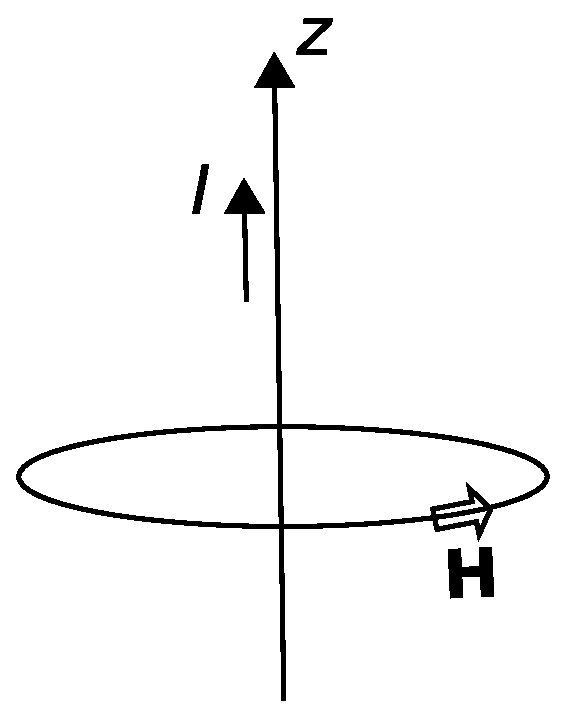
\includegraphics[width=1.5in]{modules/m0048_fBiotSavartExample.eps}
% https://commons.wikimedia.org/wiki/File:Biot_Savart_Example.svg
}}{A z-axis extends upward, with an arrow pointing in the positive z direction to indicate current direction. A circle around the z-axis shows an arrow in a counterclockwise direction labeled H to indicate magnetic field intensity.}
\end{center} 
\centerline{\scriptsize 
\copyright~\hyperref[m0048_fBiotSavartExample_Credit]{K.\ Kikkeri} 
\href{https://creativecommons.org/licenses/by-sa/4.0/}{CC BY~SA 4.0} 
} 
\caption{
\label{m0048_fBiotSavartExample}
Magnetic field intensity due to a current flowing along the $z$ axis.
}
\end{figure}
\end{example}

\index{circulation|)}

Curl is, in part, an answer to the question of what the circulation \emph{at a point in space} is.
In other words, what is the circulation as ${\mathcal C}$ shrinks to it's smallest possible size.  
The answer in one sense is zero, since the arclength of ${\mathcal C}$ is zero in this limit -- there is nothing to integrate over.
However, if we ask instead what is the circulation \emph{per unit area} in the limit, then the result should be the non-trivial value of interest. 
To express this mathematically, we constrain ${\mathcal C}$ to lie in a plane, and define ${\mathcal S}$ to be the open surface bounded by ${\mathcal C}$ in this case.
Then, we define the scalar part of the curl of ${\bf A}$ to be:
%
\begin{equation}
\lim_{\Delta s \to 0} \frac{\oint_{\mathcal C} {\bf A}\cdot d{\bf l}}{\Delta s}
\end{equation}
%
where $\Delta s$ is the area of ${\mathcal S}$, and (important!) we require ${\mathcal C}$ and ${\mathcal S}$ to lie in the plane that maximizes the above result. 

Because ${\mathcal S}$ and it's boundary ${\mathcal C}$ lie in a plane, it is possible to assign a direction to the result.
The chosen direction is the normal $\hat{\bf n}$ to the plane in which ${\mathcal C}$ and ${\mathcal S}$ lie.
Because there are two normals at each point on a plane, we specify the one that satisfies the \emph{right hand rule}.
This rule, applied to the curl, states that the correct normal is the one which points through the plane in the same direction as the fingers of the right hand when the thumb of your right hand is aligned along ${\mathcal C}$ in the direction of integration.
Why is this the correct orientation of $\hat{\bf n}$?  
See Section~\ref{m0051_Stokes_Theorem} for the answer to that question.
For the purposes of this section, it suffices to consider this to be simply an arbitrary sign convention.
  
Now with the normal vector $\hat{\bf n}$ unambiguously defined, we can now formally define the curl operation as follows:
\index{curl!definition}
%
\begin{equation}
\mbox{curl}~{\bf A} \triangleq \lim_{\Delta s \to 0} \frac{\hat{\bf n}\oint_{\mathcal C} {\bf A}\cdot d{\bf l}}{\Delta s}
\label{m0048_eCurlDef}
\end{equation}
%
where, once again, $\Delta s$ is the area of ${\mathcal S}$, and we select ${\mathcal S}$ to lie in the plane that maximizes the magnitude of the above result.  Summarizing:

%ORB HIGHLIGHT
\begin{mdframed}[backgroundcolor=yellow!20,nobreak=true] 
The curl operator quantifies the circulation of a vector field at a point.
\end{mdframed}

%ORB HIGHLIGHT
\begin{mdframed}[backgroundcolor=yellow!20,nobreak=true] 
The magnitude of the curl of a vector field is the circulation, per unit area, at a point and such that the closed path of integration shrinks to enclose zero area while being constrained to lie in the plane that maximizes the magnitude of the result.
\end{mdframed}

%ORB HIGHLIGHT
\begin{mdframed}[backgroundcolor=yellow!20,nobreak=true] 
The direction of the curl is determined by the right-hand rule applied to the associated path of integration.
\end{mdframed}

Curl is a very important operator in electromagnetic analysis.
However, the definition (Equation~\ref{m0048_eCurlDef}) is usually quite difficult to apply.
Remarkably, however, it turns out that the curl operation can be defined in terms of the $\nabla$ operator; that is, the same $\nabla$ operator associated with the gradient, divergence, and Laplacian operators.  Here is that definition:
%
\begin{equation}
\mbox{curl}~{\bf A} \triangleq \nabla \times {\bf A}
\end{equation}
%
For example:
In Cartesian coordinates,
%
\begin{equation}
\nabla \triangleq \hat{\bf x}\frac{\partial}{\partial x} + \hat{\bf y}\frac{\partial}{\partial y} + \hat{\bf z}\frac{\partial}{\partial z} 
\end{equation}
%
and
%
\begin{equation}
{\bf A} = \hat{\bf x}A_x + \hat{\bf y}A_y + \hat{\bf z}A_z 
\end{equation}
%
so curl can be calculated as follows:
%
\begin{equation}
\nabla\times{\bf A} =
\begin{vmatrix}
\hat{\bf x} & \hat{\bf y} & \hat{\bf z} \\
\frac{\partial}{\partial x} & \frac{\partial}{\partial y} & \frac{\partial}{\partial z} \\
A_x & A_y & A_z 
\end{vmatrix}
\end{equation}
%
or, evaluating the determinant:
%   
\begin{equation}
\begin{split}
\nabla \times {\bf A} &= \hat{\bf x}\left( \frac{\partial A_z}{\partial y} - \frac{\partial A_y}{\partial z} \right) \\
                      &~~ +\hat{\bf y}\left( \frac{\partial A_x}{\partial z} - \frac{\partial A_z}{\partial x} \right) \\
                      &~~ +\hat{\bf z}\left( \frac{\partial A_y}{\partial x} - \frac{\partial A_x}{\partial y} \right) 
\end{split}
\end{equation}
%
Expressions for curl in each of the three major coordinate systems is provided in Appendix~\ref{m0139_Vector_Operators}. 

It is useful to know is that curl, like $\nabla$ itself, is a linear operator; that is, for any constant scalars $a$ and $b$ and vector fields ${\bf A}$ and ${\bf B}$:
%
\begin{equation}
\nabla \times \left( a{\bf A} + b{\bf B} \right) = a \nabla \times {\bf A} + b \nabla \times {\bf B}
\end{equation}

%%%%%%%%%%%%%%%%%%%%%%%%%%%%%%%%%%%%

{\bf Additional Reading:}
\begin{itemize}
\item ``\href{https://en.wikipedia.org/wiki/Curl_(mathematics)}{Curl (mathematics)}'' on Wikipedia.
\end{itemize}

\index{curl|)}



      \vfill\break
    \section{Stokes' Theorem}
{\color{blue}\tiny[m0051]}      % This is text associated with the open textbook "Open Electromagnetics"
% See immediately below for author, date
% This work is licensed under the Creative Commons Attribution-ShareAlike 4.0 International License. (CC BY-SA 4.0) 
% To view a copy of the license, visit http://creativecommons.org/licenses/by-sa/4.0/

%ORB TITLE Stokes' Theorem 
%ORB AUTHOR 0        # S.W. Ellingson, Virginia Tech (ellingson@vt.edu)
%ORB DATE 20180803   # yyyymmdd
%ORB ABSTRACT 

\label{m0051_Stokes_Theorem} % <-- Must match name of this file and module directory name.  Don't mess with this!
\index{Stokes' theorem|(}

\emph{Stokes' Theorem} relates an integral over an open surface to an integral over the curve bounding that surface.
This relationship has a number of applications in electromagnetic theory.
Here is the theorem:
%
\begin{equation} 
\boxed{  
\int_{\mathcal S} \left( \nabla \times {\bf A} \right) \cdot d{\bf s} = \oint_{\mathcal C} {\bf A}\cdot d{\bf l}
}
\end{equation}
%
where $\mathcal{S}$ is the open surface bounded by the closed path $\mathcal{C}$.
The direction of the surface normal $d{\bf s}=\hat{\bf n}ds$ is related to the direction of integration along ${\mathcal C}$ by the \emph{right-hand rule}, 
\index{right-hand rule!Stokes' theorem}
illustrated in Figure~\ref{m0051_fStokesRHR}.
In this case, the right-hand rule states that the correct normal is the one that points through the surface in the same direction as the fingers of the right hand when the thumb of your right hand is aligned along ${\mathcal C}$ in the direction of integration. 
%
\begin{figure}[b!]
\begin{center}
\pdftooltip{{  % note double braces
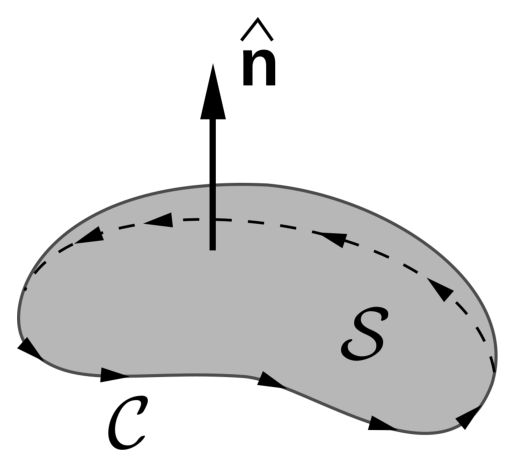
\includegraphics[width=1.5in]{modules/m0051_fStokesRHR.eps}
% https://en.wikipedia.org/wiki/File:Stokes'_Theorem.svg
}}{A curved surface with circumference labeled C, surface area labeled S, and normal vector pointing perpendicular to the surface. }
\end{center} 
\centerline{\scriptsize 
\copyright~\hyperref[m0051_fStokesRHR_Credit]{Cronholm144} (modified)
\href{https://creativecommons.org/licenses/by-sa/3.0/}{CC BY~SA 3.0} 
} 
\caption{
\label{m0051_fStokesRHR}
The relative orientations of the direction of integration ${\mathcal C}$ and surface normal $\hat{\bf n}$ in Stokes' Theorem.
}
\end{figure}

Stokes' Theorem is a purely mathematical result and not a principle of electromagnetics \emph{per se}.
The relevance of the theorem to electromagnetic theory is primarily as a tool in the associated mathematical analysis.
Usually the theorem is employed to transform a problem expressed in terms of an integration over a surface into an integration over a closed path or vice-versa.
For more information on the theorem and its derivation, see ``Additional Reading'' at the end of this section.

%%%%%%%%%%%%%%%%%%%%%%%%%%%%%%%%%%%%

{\bf Additional Reading:}
\begin{itemize}
\item ``\href{https://en.wikipedia.org/wiki/Stokes'_theorem}{Stokes' Theorem}'' on Wikipedia.
\end{itemize}

\index{Stokes' theorem|)}



      \vfill\break
    \section{The Laplacian Operator}
{\color{blue}\tiny[m0099]}      % This is text associated with the open textbook "Open Electromagnetics"
% See immediately below for author, date
% This work is licensed under the Creative Commons Attribution-ShareAlike 4.0 International License. (CC BY-SA 4.0) 
% To view a copy of the license, visit http://creativecommons.org/licenses/by-sa/4.0/

%ORB TITLE The Laplacian Operator
%ORB AUTHOR 0        # S.W. Ellingson, Virginia Tech (ellingson@vt.edu)
%ORB DATE 20180609   # yyyymmdd
%ORB ABSTRACT

\label{m0099_The_Laplacian_Operator} % <-- Must match name of this file and module directory name.  Don't mess with this!
\index{Laplacian (operator)|(}

The Laplacian $\nabla^2 f$ of a field $f({\bf r})$ is the divergence of the gradient of that field:
%
\begin{equation}
\nabla^2 f \triangleq \nabla\cdot\left(\nabla f\right)
\label{m0099_eLaplaceDef}
\end{equation}
%
Note that the Laplacian is essentially a definition of the second derivative with respect to the three spatial dimensions.
For example, in Cartesian coordinates,
%
\begin{equation}
\nabla^2 f= 
\frac{\partial^2 f}{\partial x^2}  
+ \frac{\partial^2 f}{\partial y^2}  
+ \frac{\partial^2 f}{\partial z^2} 
\label{m0099_eLaplaceScalar} 
\end{equation}
%
as can be readily verified by applying the definitions of gradient and divergence in Cartesian coordinates to Equation~\ref{m0099_eLaplaceDef}.

The Laplacian relates the
electric potential (i.e., $V$, units of V) to electric charge density (i.e., $\rho_v$, units of C/m$^3$).
This relationship is known as {\it Poisson's Equation} 
\index{Poisson's equation}
(Section~\ref{m0067_Poissons_and_Laplaces_Equations}):
%
\begin{equation}
\nabla^2 V = - \frac{\rho_v}{\epsilon}
\end{equation}  
%
where $\epsilon$ is the permittivity of the medium.
The fact that $V$ is related to $\rho_v$ in this way should not be surprising, since electric field intensity $({\bf E}$, units of V/m) is proportional to the derivative of $V$ with respect to distance (via the gradient) and $\rho_v$ is proportional to the derivative of ${\bf E}$ with respect to distance (via the divergence).

The Laplacian operator can also be applied to \emph{vector} fields; for example, Equation~\ref{m0099_eLaplaceScalar} is valid even if the scalar field ``$f$'' is replaced with a vector field.  
In the Cartesian coordinate system, the Laplacian of the vector field ${\bf A} = \hat{\bf x}A_x + \hat{\bf y}A_y + \hat{\bf z}A_z$ is
%
\begin{equation}
\nabla^2 {\bf A} = \hat{\bf x}\nabla^2 A_x + \hat{\bf y}\nabla^2 A_y + \hat{\bf z}\nabla^2 A_z
\end{equation}
%
An important application of the Laplacian operator of vector fields is the \emph{wave equation}; 
\index{wave equation!electromagnetic}
e.g., the wave equation for ${\bf E}$ in a lossless and source-free region is (Section~\ref{m0036_Wave_Equations_SourceFree_Lossless})
%
\begin{equation}
\nabla^2{\bf E} + \beta^2{\bf E} = 0
\end{equation}
%
where $\beta$ is the phase propagation constant.

It is sometimes useful to know that the Laplacian of a vector field can be expressed in terms of the gradient, divergence, and curl as follows:
%
\begin{equation}
\nabla^2 {\bf A} = \nabla\left(\nabla\cdot{\bf A}\right) - \nabla\times\left(\nabla\times{\bf A}\right)
\end{equation}

The Laplacian operator in the cylindrical and spherical coordinate systems is given in Appendix~\ref{m0139_Vector_Operators}.

%%%%%%%%%%%%%%%%%%%%%%%%%%%%%%%%%%%%

{\bf Additional Reading:}
\begin{itemize}
\item ``\href{https://en.wikipedia.org/wiki/Laplace_operator}{Laplace operator}'' on Wikipedia.
\end{itemize}

\index{Laplacian (operator)|)}

%%%      \vfill\break
{\color{blue}\tiny[m0043]}    % This is text associated with the open textbook "Open Electromagnetics"
% See immediately below for author, date
% This work is licensed under the Creative Commons Attribution-ShareAlike 4.0 International License. (CC BY-SA 4.0) 
% To view a copy of the license, visit http://creativecommons.org/licenses/by-sa/4.0/

%ORB TITLE Image Credits
%ORB AUTHOR 0        # S.W. Ellingson, Virginia Tech (ellingson@vt.edu)
%ORB DATE 20180701   # yyyymmdd
%ORB ABSTRACT End matter for chapter entitled "Vector Analysis"

\label{m0043_Ch_End_Matter_Vector_Analysis} % <-- Must match name of this file and module directory name.  Don't mess with this!

\onecolumn
\section*{Image Credits}

\begin{itemize}

\item[Fig.] \label{m0006_fCartesian_Credit}
  \ref{m0006_fCartesian}:
  \copyright~K.\ Kikkeri, 
  \url{https://commons.wikimedia.org/wiki/File:M0006_fCartesian.svg},\\ 
  CC BY~SA 4.0 (\url{https://creativecommons.org/licenses/by-sa/4.0/}).

\item[Fig.] \label{m0006_fPositionFixed_Credit}
  \ref{m0006_fPositionFixed}:
  \copyright~K.\ Kikkeri, 
  \url{https://commons.wikimedia.org/wiki/File:M0006_fPositionFixed.svg},\\ 
  CC BY~SA 4.0 (\url{https://creativecommons.org/licenses/by-sa/4.0/}).

\item[Fig.] \label{m0006_fPositionFree_Credit}
  \ref{m0006_fPositionFree}:
  \copyright~K.\ Kikkeri, 
  \url{https://commons.wikimedia.org/wiki/File:M0006_fPositionFree.svg},\\ 
  CC BY~SA 4.0 (\url{https://creativecommons.org/licenses/by-sa/4.0/}).

\item[Fig.] \label{m0006_fCartesianBasis_Credit}
  \ref{m0006_fCartesianBasis}:
  \copyright~K.\ Kikkeri, 
  \url{https://commons.wikimedia.org/wiki/File:M0006_fCartesianBasis.svg},\\ 
  CC BY~SA 4.0 (\url{https://creativecommons.org/licenses/by-sa/4.0/}).

\item[Fig.] \label{m0006_fVecCart_Credit}
  \ref{m0006_fVecCart}:
  \copyright~K.\ Kikkeri, 
  \url{https://commons.wikimedia.org/wiki/File:M0006_fVecCart.svg},\\ 
  CC BY~SA 4.0 (\url{https://creativecommons.org/licenses/by-sa/4.0/}).

\item[Fig.] \label{m0006_fRelativePosition_Credit}
  \ref{m0006_fRelativePosition}:
  \copyright~K.\ Kikkeri, 
  \url{https://commons.wikimedia.org/wiki/File:M0006_fRelativePosition.svg},\\ 
  CC BY~SA 4.0 (\url{https://creativecommons.org/licenses/by-sa/4.0/}).

\item[Fig.] \label{m0006_fDotProductSpecialCases_Credit}
  \ref{m0006_fDotProductSpecialCases}:
  \copyright~K.\ Kikkeri, 
  \url{https://commons.wikimedia.org/wiki/File:M0006_fDotProductSpecialCases.svg},\\ 
  CC BY~SA 4.0 (\url{https://creativecommons.org/licenses/by-sa/4.0/}).

\item[Fig.] \label{m0006_fDotProduct_Credit}
  \ref{m0006_fDotProduct}:
  \copyright~K.\ Kikkeri, 
  \url{https://commons.wikimedia.org/wiki/File:M0006_fDotProduct.svg},\\ 
  CC BY~SA 4.0 (\url{https://creativecommons.org/licenses/by-sa/4.0/}).

\item[Fig.] \label{m0006_fCrossProduct_Credit}
  \ref{m0006_fCrossProduct}:
  \copyright~K.\ Kikkeri, 
  \url{https://commons.wikimedia.org/wiki/File:M0006_fCrossProduct.svg},\\ 
  CC BY~SA 4.0 (\url{https://creativecommons.org/licenses/by-sa/4.0/}).

\item[Fig.] \label{m0096_fCylindricalCoordinates_Credit}
  \ref{m0096_fCylindricalCoordinates}:
  \copyright~K.\ Kikkeri, 
  \url{https://commons.wikimedia.org/wiki/File:M0096_fCylindricalCoordinates.svg},\\ 
  CC BY~SA 4.0 (\url{https://creativecommons.org/licenses/by-sa/4.0/}).

\item[Fig.] \label{m0096_Circle_Credit}
  \ref{m0096_Circle}:
  \copyright~K.\ Kikkeri, 
  \url{https://commons.wikimedia.org/wiki/File:Cylindrical_Coordinates_Example.svg},\\ 
  CC BY~SA 4.0 (\url{https://creativecommons.org/licenses/by-sa/4.0/}).

\item[Fig.] \label{m0096_CircleArea_Credit}
  \ref{m0096_CircleArea}:
  \copyright~K.\ Kikkeri, 
  \url{https://commons.wikimedia.org/wiki/File:Cylindrical_Coordinates-Area_of_a_Circle.svg},\\ 
  CC BY~SA 4.0 (\url{https://creativecommons.org/licenses/by-sa/4.0/}).

\item[Fig.] \label{m0096_CylinderArea_Credit}
  \ref{m0096_CylinderArea}:
  \copyright~K.\ Kikkeri, 
  \url{https://commons.wikimedia.org/wiki/File:M0096_CylinderArea.svg},\\ 
  CC BY~SA 4.0 (\url{https://creativecommons.org/licenses/by-sa/4.0/}).

\item[Fig.] \label{m0097_fSphericalCoordinates_Credit}
  \ref{m0097_fSphericalCoordinates}:
  \copyright~K.\ Kikkeri, 
  \url{https://commons.wikimedia.org/wiki/File:Spherical_Coordinate_System.svg},\\ 
  CC BY~SA 4.0 (\url{https://creativecommons.org/licenses/by-sa/4.0/}).

\item[Fig.] \label{m0097_fArc_Credit}
  \ref{m0097_fArc}:
  \copyright~K.\ Kikkeri, 
  \url{https://commons.wikimedia.org/wiki/File:M0097_fArc.svg},\\ 
  CC BY~SA 4.0 (\url{https://creativecommons.org/licenses/by-sa/4.0/}).

\item[Fig.] \label{m0097_fSphereArea_Credit}
  \ref{m0097_fSphereArea}:
  \copyright~K.\ Kikkeri, 
  \url{https://commons.wikimedia.org/wiki/File:M0097_fSphereArea.svg},\\ 
  CC BY~SA 4.0 (\url{https://creativecommons.org/licenses/by-sa/4.0/}).

\item[Fig.] \label{m0048_fBiotSavartExample_Credit}
  \ref{m0048_fBiotSavartExample}:
  \copyright~K.\ Kikkeri, 
  \url{https://commons.wikimedia.org/wiki/File:Biot_Savart_Example.svg},\\ 
  CC BY~SA 4.0 (\url{https://creativecommons.org/licenses/by-sa/4.0/}).

\item[Fig.] \label{m0051_fStokesRHR_Credit}
  \ref{m0051_fStokesRHR}:
  \copyright~Cronholm144, 
  \url{https://en.wikipedia.org/wiki/File:Stokes'_Theorem.svg},\\ 
  CC BY~SA 3.0 (\url{https://creativecommons.org/licenses/by-sa/3.0/}).
  Heavily modified by author.

\end{itemize}

\twocolumn

  \chapter{Electrostatics}
  \thispagestyle{fancy} % override footer in first page of chapter
  \fancyhf{}            % reset header and footer
  \fancyfoot[C]{\footnotesize \emph{Electromagnetics Vol~1}. ~\copyright~2018 S.W.\ Ellingson ~CC~BY~SA~4.0. ~\url{https://doi.org/10.21061/electromagnetics-vol-1}}
{\color{blue}\tiny[m0116]}    % This is text associated with the open textbook "Open Electromagnetics"
% See immediately below for author, date
% This work is licensed under the Creative Commons Attribution-ShareAlike 4.0 International License. (CC BY-SA 4.0) 
% To view a copy of the license, visit http://creativecommons.org/licenses/by-sa/4.0/

%ORB TITLE Electrostatics
%ORB AUTHOR 0        # S.W. Ellingson, Virginia Tech (ellingson@vt.edu)
%ORB DATE 20180803   # yyyymmdd
%ORB ABSTRACT Electrostatics 

\label{m0116_Electrostatics_Preface} % <-- Must match name of this file and module directory name.  Don't mess with this!
\index{electrostatics (description)|(}

\emph{Electrostatics} is the theory of the electric field in conditions in which its behavior is independent of magnetic fields, including
%
\begin{itemize}
\item The electric field associated with fixed distributions of electric charge
\item \emph{Capacitance} (the ability of a structure to store energy in an electric field)
\item The \emph{energy} associated with the electrostatic field
\item \emph{Steady current} induced in a conducting material in the presence of an electrostatic field (essentially, Ohm's Law)
\end{itemize}
%
The term ``static'' refers to the fact that these aspects of electromagnetic theory can be developed by assuming sources are time-invariant; we might say that electrostatics is the study of the electric field at DC.  However, many aspects of electrostatics are relevant to AC, radio frequency, and higher-frequency applications as well.
 
%%%%%%%%%%%%%%%%%%%%%%%%%%%%%%%%%%%%%%%%

{\bf Additional Reading:}
\begin{itemize}
\item ``\href{https://en.wikipedia.org/wiki/Electrostatics}{Electrostatics}'' on Wikipedia.
\end{itemize}

\index{electrostatics (description)|)}


\vspace{1in}

    \section{Coulomb's Law}
{\color{blue}\tiny[m0102]}      % This is text associated with the open textbook "Open Electromagnetics"
% See immediately below for author, date
% This work is licensed under the Creative Commons Attribution-ShareAlike 4.0 International License. (CC BY-SA 4.0) 
% To view a copy of the license, visit http://creativecommons.org/licenses/by-sa/4.0/

%ORB TITLE Coulomb's Law
%ORB AUTHOR 0        # S.W. Ellingson, Virginia Tech (ellingson@vt.edu)
%ORB DATE 20180803   # yyyymmdd
%ORB ABSTRACT Coulomb's Law

\label{m0102_Coulombs_Law} % <-- Must match name of this file and module directory name.  Don't mess with this!
\index{Coulomb's law|(}

Consider two charge-bearing particles in free space, identified as ``particle~1'' and ``particle~2'' in Figure~\ref{m0102_fCoulombsLaw}.
Let the charges borne by these particles be $q_1$ and $q_2$, and let $R$  be the distance between them.
If the particles bear charges of the same sign (i.e., if $q_1q_2$ is positive), then the particles repel; otherwise, they attract.
This repulsion or attraction can be quantified as a force experienced by each particle.  
Physical observations reveal that the magnitude of the force is proportional to $q_1q_2$, and inversely proportional to $R^2$.
For particle~2 we find:
%
\begin{equation}
{\bf F} = \hat{\bf R} F_0 \frac{q_1 q_2}{R^2}
\end{equation}
%
where 
$\hat{\bf R}$ is the unit vector pointing from the particle~1 to the particle~2, and
$F_0$ is a constant.  
The value of $F_0$ must have units of inverse permittivity; i.e., 
(F/m)$^{-1}$.
This is most easily seen by dimensional analysis of the above relationship, including the suspected factor:
\begin{equation}
\frac{\mbox{C}\cdot\mbox{C}}{\mbox{F/m}\cdot\mbox{m}^2} 
= \frac{\mbox{C}\cdot\mbox{C}}{\mbox{F}\cdot\mbox{m}} 
= \frac{\mbox{C}\cdot\mbox{C}}{\mbox{C/V}\cdot\mbox{m}}
= \frac{\mbox{C}\cdot\mbox{V}}{\mbox{m}}
= \frac{\mbox{J}}{\mbox{m}}
= \mbox{N}
\nonumber
\end{equation}
%
where we have used the facts that 
1~F $=$ 1~C/V,
1~V $=$ 1~J/C, and
1~N $=$ 1~J/m.
%
This finding suggests that $F_0\propto\epsilon^{-1}$, where $\epsilon$ is the permittivity of the medium in which the particles exist.
Observations confirm that the force is in fact inversely proportional to the permittivity, with an additional factor of $1/4\pi$ (unitless).  
Putting this all together we obtain what is commonly known as \emph{Coulomb's Law}:
%
\begin{equation}
\boxed{
{\bf F} = \hat{\bf R}\frac{q_1 q_2}{4\pi\epsilon R^2}
}
\end{equation} 
%
\begin{figure}
\begin{center}
\pdftooltip{{  % note double braces
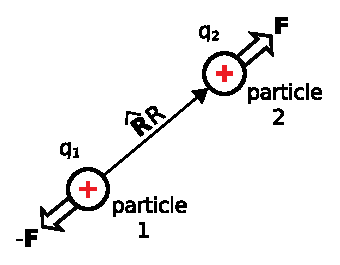
\includegraphics[width=2in]{modules/m0102_fCoulombsLaw.eps}
% https://commons.wikimedia.org/wiki/File:M0102_fCoulombsLaw.svg
}}{The diagram shows two positively-charged particles, particle 1 and particle 2, represented by two circles with red plus signs in the middle. Particle 1 is also labeled q sub 1, and particle 2 is also labeled q sub 2. The distance between them is separated by an arrow pointing from particle 1 to particle 2, labeled bold R-hat * R. An arrow pointing away from particle 1 is labeled -F. An arrow pointing away from particle 2 is labeled F. }
\end{center} 
\centerline{\scriptsize 
\copyright~\hyperref[m0102_fCoulombsLaw_Credit]{K. Kikkeri} 
\href{https://creativecommons.org/licenses/by-sa/4.0/}{CC BY~SA 4.0} 
} 
\caption{
\label{m0102_fCoulombsLaw}
Coulomb's Law describes the force perceived by pairs of charged particles.
}
\end{figure}

Subsequently, the force perceived by particle~2 is equal and opposite; i.e., equal to $-{\bf F}$.
 
Separately, it is known that ${\bf F}$ can be described in terms of the electric field intensity ${\bf E}_1$ associated with particle~1:
%
\begin{equation}
{\bf F} = q_2{\bf E}_1
\end{equation} 
%
This is essentially the \emph{definition} of ${\bf E}_1$, as explained in Section~\ref{m0002_Electric_Field_Intensity}.
Combining this result with Coulomb's Law, we obtain a means to directly calculate the field associated with the first particle in the absence of the second particle:
%
\begin{equation}
\boxed{
{\bf E}_1 = \hat{\bf R}\frac{q_1}{4\pi\epsilon R^2}
}
\label{m0102_eCoulombsLawPointCharge}
\end{equation} 
%
where now $\hat{\bf R}R$ is the vector beginning at the particle~1 and ending at the point to be evaluated.

%--------------------------------
%ORB HIGHLIGHT
\begin{mdframed}[backgroundcolor=yellow!20,nobreak=true] 
The electric field intensity 
\index{electric field intensity}
associated with a point charge (Equation~\ref{m0102_eCoulombsLawPointCharge}) is (1) directed away from positive charge, (2) proportional to the magnitude of the charge, (3) inversely proportional to the permittivity of the medium, and (3) inversely proportional to distance squared. 
\end{mdframed}
%--------------------------------

We have described this result as originating from Coulomb's Law, which is based on physical observations.
However, the same result may be obtained directly from Maxwell's Equations using Gauss' Law (Section~\ref{m0014_Gauss_Law_Integral_Form}).

%--------------------------------
%ORB EXAMPLE
~\\ \begin{example} 
\begin{mdframed}[backgroundcolor=brown!20,linecolor=brown!20]\raggedright
Electric field of a point charge at the origin.
\\~\\
A common starting point in electrostatic analysis is the field associated with a particle bearing charge $q$ at the origin of the coordinate system.
Because the electric field is directed radially away from a positively-charged source particle in all directions, this field is most conveniently described in the spherical coordinate system.
Thus, $\hat{\bf R}$ becomes $\hat{\bf r}$, $R$ becomes $r$, and we have
%
\begin{equation}
{\bf E}({\bf r}) = \hat{\bf r}\frac{q}{4\pi\epsilon r^2}
\end{equation} 

Here's a numerical example. What is the electric field intensity at a distance 1~$\mu$m from a single electron located at the origin, in free space?
In this case, $q\cong -1.60 \times 10^{-19}$~C (don't forget that minus sign!), $\epsilon=\epsilon_0$, $r=1~\mu$m, and we find: 
%
\begin{equation}
{\bf E}({\bf r}) = -\hat{\bf r}\left(1.44~\mbox{kV/m}\right)
\end{equation} 
%
This is large relative to electric field strengths commonly encountered in engineering applications.
The strong electric field of the electron is not readily apparent because electrons in common materials tend to be accompanied by roughly equal amounts of positive charge, such as the protons of atoms.
Sometimes, however, the effect of individual electrons {\it does} become significant in practical electronics through a phenomenon known as \emph{shot noise}.
\index{shot noise}
\end{mdframed}\end{example}
%--------------------------------

{\bf Additional Reading:}
\begin{itemize}
\item ``\href{https://en.wikipedia.org/wiki/Coulomb's_law}{Coulomb's Law}'' on Wikipedia.
\item ``\href{https://en.wikipedia.org/wiki/Shot_noise}{Shot Noise}'' on Wikipedia.
\end{itemize}

\index{Coulomb's law|)}

      \vfill\break
    \section{Electric Field Due to Point Charges}
{\color{blue}\tiny[m0103]}      % This is text associated with the open textbook "Open Electromagnetics"
% See immediately below for author, date
% This work is licensed under the Creative Commons Attribution-ShareAlike 4.0 International License. (CC BY-SA 4.0) 
% To view a copy of the license, visit http://creativecommons.org/licenses/by-sa/4.0/

%ORB TITLE Electric Field Due to Point Charges
%ORB AUTHOR 0        # S.W. Ellingson, Virginia Tech (ellingson@vt.edu)
%ORB DATE 20180803   # yyyymmdd
%ORB ABSTRACT Electric Field Due to Point Charges

\label{m0103_E_due_to_Point_Charges} % <-- Must match name of this file and module directory name.  Don't mess with this!

The electric field intensity associated with a single particle bearing charge $q_1$, located at the origin, is (Section~\ref{m0102_Coulombs_Law})
%
\begin{equation}
{\bf E}({\bf r}) = \hat{\bf r}\frac{q_1}{4\pi\epsilon r^2}
\end{equation} 
%
If this particle is instead located at some position ${\bf r}_1$, then the above expression may be written as follows:
%
\begin{equation}
{\bf E}({\bf r};{\bf r}_1) = \frac{{\bf r}-{\bf r}_1}{\left|{\bf r}-{\bf r}_1\right|}~\frac{q_1}{4\pi\epsilon \left|{\bf r}-{\bf r}_1\right|^2}
\end{equation} 
%
or, combining like terms in the denominator:
%
\begin{equation}
{\bf E}({\bf r};{\bf r}_1) = \frac{{\bf r}-{\bf r}_1}{\left|{\bf r}-{\bf r}_1\right|^3}~\frac{q_1}{4\pi\epsilon}
\end{equation} 

Now let us consider the field due to multiple such particles.
Under the usual assumptions about the permittivity of the medium (reminder: Section~\ref{m0007_Properties_of_Materials}), the property of superposition applies.
Using this principle, we conclude: 
%
%ORB HIGHLIGHT
\begin{mdframed}[backgroundcolor=yellow!20,nobreak=true] 
The electric field resulting from a set of charged particles is equal to the sum of the fields associated with the individual particles.
\end{mdframed}
%
Stated mathematically:
%
\begin{equation}
{\bf E}({\bf r}) = \sum_{n=1}^{N}{\bf E}({\bf r};{\bf r}_n)
\end{equation} 
%
where $N$ is the number of particles.
Thus, we have
%
\begin{equation}
{\bf E}({\bf r}) = \frac{1}{4\pi\epsilon} \sum_{n=1}^{N} {   \frac{{\bf r}-{\bf r}_n}{\left|{\bf r}-{\bf r}_n\right|^3}~q_n}
\end{equation} 

% TODO: complete example below.
% %ORB EXAMPLE
% ~\\ \begin{example} 
% \begin{mdframed}[backgroundcolor=green!20] 
% Electric Dipole
% \end{mdframed}
% {\color{red}NEEDS TO BE COMPLETED.}
% \centerline{\rule{2in}{1pt}} \end{example}






      \vfill\break
    \section{Charge Distributions}
{\color{blue}\tiny[m0100]}      % This is text associated with the open textbook "Open Electromagnetics"
% See immediately below for author, date
% This work is licensed under the Creative Commons Attribution-ShareAlike 4.0 International License. (CC BY-SA 4.0) 
% To view a copy of the license, visit http://creativecommons.org/licenses/by-sa/4.0/

%ORB TITLE Charge Distributions
%ORB AUTHOR 0        # S.W. Ellingson, Virginia Tech (ellingson@vt.edu)
%ORB DATE 20180803   # yyyymmdd
%ORB ABSTRACT Charge Distributions 

\label{m0100_Charge_Distributions} % <-- Must match name of this file and module directory name.  Don't mess with this!

In principle, the smallest unit of electric charge that can be isolated is the charge of a single electron, which is $\cong -1.60 \times 10^{-19}$~C.
This is very small, and we rarely deal with electrons one at a time, so it is usually more convenient to describe charge as a quantity that is continuous over some region of space.  In particular, it is convenient to describe charge as being distributed in one of three ways: along a curve, over a surface, or within a volume.

{\bf Line Charge Distribution.} 
\index{charge density!line}
Imagine that charge is distributed along a curve ${\mathcal C}$ through space.   
Let $\Delta q$ be the total charge along a short segment of the curve, and let $\Delta l$ be the length of this segment.
The \emph{line charge density} $\rho_l$ at any point along the curve is defined as
%
\begin{equation}
\rho_l \triangleq \lim_{\Delta l \to 0} \frac{\Delta q}{\Delta l} = \frac{dq}{dl}
\end{equation}
%
which has units of C/m.
We may then define $\rho_l$ to be a function of position along the curve, parameterized by $l$; e.g., $\rho_l(l)$.
Then, the total charge $Q$ along the curve is
%
\begin{equation}
Q = \int_{\mathcal C} \rho_l(l)~dl
\end{equation}
%
which has units of C.
In other words, line charge density integrated over length yields total charge.

{\bf Surface Charge Distribution.} 
\index{charge density!surface}
Imagine that charge is distributed over a surface.   
Let $\Delta q$ be the total charge on a small patch on this surface, and let $\Delta s$ be the area of this patch.
The \emph{surface charge density} $\rho_s$ at any point on the surface is defined as
%
\begin{equation}
\rho_s \triangleq \lim_{\Delta s \to 0} \frac{\Delta q}{\Delta s} = \frac{dq}{ds}
\end{equation}
%
which has units of C/m$^2$.
Let us define $\rho_s$ to be a function of position on this surface.
Then the total charge over a surface ${\mathcal S}$ is
%
\begin{equation}
Q = \int_{\mathcal S} \rho_s~ds
\end{equation}
%
In other words, surface charge density integrated over a surface yields total charge.

{\bf Volume Charge Distribution.} 
\index{charge density!volume}
Imagine that charge is distributed over a volume.   
Let $\Delta q$ be the total charge in a small cell within this volume, and let $\Delta v$ be the volume of this cell.
The \emph{volume charge density} $\rho_v$ at any point in the volume is defined as
%
\begin{equation}
\rho_v \triangleq \lim_{\Delta v \to 0} \frac{\Delta q}{\Delta v} = \frac{dq}{dv}
\end{equation}
%
which has units of C/m$^3$.
Since $\rho_v$ is a function of position within this volume, the total charge within a volume ${\mathcal V}$ is
%
\begin{equation}
Q = \int_{\mathcal V} \rho_v~dv
\end{equation}
%
In other words, volume charge density integrated over a volume yields total charge.


      \vfill\break
    \section{Electric Field Due to a Continuous Distribution of Charge}
{\color{blue}\tiny[m0104]}      % This is text associated with the open textbook "Open Electromagnetics"
% See immediately below for author, date
% This work is licensed under the Creative Commons Attribution-ShareAlike 4.0 International License. (CC BY-SA 4.0) 
% To view a copy of the license, visit http://creativecommons.org/licenses/by-sa/4.0/

%ORB TITLE Electric Field Due to a Continuous Distribution of Charge
%ORB AUTHOR 0        # S.W. Ellingson, Virginia Tech (ellingson@vt.edu)
%ORB DATE 20180803   # yyyymmdd
%ORB ABSTRACT Electric Field Due to a Continuous Distribution of Charge

\label{m0104_E_due_to_a_Continuous_Distribution_of_Charge} % <-- Must match name of this file and module directory name.  Don't mess with this!

The electric field intensity associated with $N$ charged particles is (Section~\ref{m0103_E_due_to_Point_Charges}):
%
\begin{equation}
{\bf E}({\bf r}) = \frac{1}{4\pi\epsilon} \sum_{n=1}^{N} {   \frac{{\bf r}-{\bf r}_n}{\left|{\bf r}-{\bf r}_n\right|^3}~q_n}
\label{m0104_eCountable}
\end{equation}
%
where $q_n$ and ${\bf r}_n$ are the charge and position of the $n^{\mbox{th}}$ particle.
However, it is common to have a continuous distribution of charge as opposed to a countable number of charged particles.
In this section, we extend Equation~\ref{m0104_eCountable} using the concept of continuous distribution of charge (Section~\ref{m0100_Charge_Distributions}) so that we may address this more general class of problems.

%---------------------------------------------------

{\bf Distribution of Charge Along a Curve.}
\index{charge density!line}
Consider a continuous distribution of charge along a curve $\mathcal{C}$.
The curve can be divided into short segments of length $\Delta l$.  
Then, the charge associated with the $n^{\mbox{th}}$ segment, located at ${\bf r}_n$, is
%
\begin{equation}
q_n = \rho_l({\bf r}_n)~\Delta l
\end{equation}
%
where $\rho_l$ is charge density (units of C/m) at ${\bf r}_n$.
Substituting this expression into Equation~\ref{m0104_eCountable}, we obtain
%
\begin{equation}
{\bf E}({\bf r}) = \frac{1}{4\pi\epsilon} \sum_{n=1}^{N} {   \frac{{\bf r}-{\bf r}_n}{\left|{\bf r}-{\bf r}_n\right|^3}~\rho_l({\bf r}_n)~\Delta l}
\end{equation}
%
Taking the limit as $\Delta l\to 0$ yields:
%
\begin{equation}
\boxed{
{\bf E}({\bf r}) = \frac{1}{4\pi\epsilon} \int_{\mathcal C} {   \frac{{\bf r}-{\bf r}'}{\left|{\bf r}-{\bf r}'\right|^3}~\rho_l({\bf r}')~dl}
}
\label{m0104_eLineCharge}
\end{equation}
%
where ${\bf r}'$ represents the varying position along ${\mathcal C}$ with integration.

The simplest example of a curve is a straight line.
It is straightforward to use Equation~\ref{m0104_eLineCharge} to determine the electric field due to a distribution of charge along a straight line.
However, it is much easier to analyze that particular distribution using Gauss' Law, as shown in Section~\ref{m0149_E_due_to_Inf_Line_Charge}.
The following example addresses a charge distribution for which Equation~\ref{m0104_eLineCharge} is more appropriate.

%ORB EXAMPLE
~\\ \begin{example} 
\begin{mdframed}[backgroundcolor=brown!20,linecolor=brown!20]\raggedright
Electric field along the axis of a ring of uniformly-distributed charge.
\\~\\
Consider a ring of radius $a$ in the $z=0$ plane, centered on the origin, as shown in Figure~\ref{m0104_fRing}.
Let the charge density along this ring be uniform and equal to $\rho_l$ (C/m).
Find the electric field along the $z$ axis.

{\bf Solution.}
The source charge position is given in cylindrical coordinates as
%
\begin{equation}
{\bf r}' = \hat{\bf \rho}a  
\end{equation}
%
The position of a field point along the $z$ axis is simply
%
\begin{equation}
{\bf r} = \hat{\bf z}z  
\end{equation}
%
Thus,
%
\begin{equation}
{\bf r}-{\bf r}' = -\hat{\bf \rho}a + \hat{\bf z}z  
\end{equation}
%
and
%
\begin{equation}
\left|{\bf r}-{\bf r}'\right| = \sqrt{a^2+z^2} 
\end{equation}

Equation~\ref{m0104_eLineCharge} becomes:
%
\begin{equation}
{\bf E}(z) = \frac{1}{4\pi\epsilon} \int_{0}^{2\pi} { \frac{-\hat{\bf \rho}a + \hat{\bf z}z}{\left[a^2+z^2\right]^{3/2}}~\rho_l~\left(a~d\phi\right)}
\end{equation}
%
Pulling factors that do not vary with $\phi$ out of the integral and factoring into separate integrals for the $\hat{\bf \phi}$ and $\hat{\bf z}$ components, we obtain:
%
\begin{equation}
\frac{\rho_l~a}{4\pi\epsilon\left[a^2+z^2\right]^{3/2}} \left[ -a\int_{0}^{2\pi}{\hat{\bf \rho}~d\phi} 
                                                               +\hat{\bf z}z\int_{0}^{2\pi} {d\phi}  \right] 
\end{equation}
%
The second integral is equal to $2\pi$.
The first integral is equal to zero.
To see this, note that the integral is simply summing values of $\hat{\bf\rho}$ for all possible values of $\phi$.  
Since $\hat{\bf\rho}(\phi+\pi)=-\hat{\bf\rho}(\phi)$, the integrand for any given value of $\phi$ is equal and opposite the integrand $\pi$ radians later.
(This is one example of a \emph{symmetry} argument.)  
Thus, we obtain
%
\begin{equation}
{\bf E}(z) = \hat{\bf z}\frac{\rho_l~a}{2\epsilon}\frac{z}{\left[a^2+z^2\right]^{3/2}} 
\end{equation}
%
It is a good exercise to confirm that this result is dimensionally correct.
% *** TODO Above as a problem. 
It is also recommended to confirm that when $z\gg a$, the result is approximately the same as that expected from a particle having the same total charge as the ring.
% *** TODO Above as a problem.
\end{mdframed}
%
\begin{figure}
\begin{center}
\pdftooltip{{  % note double braces
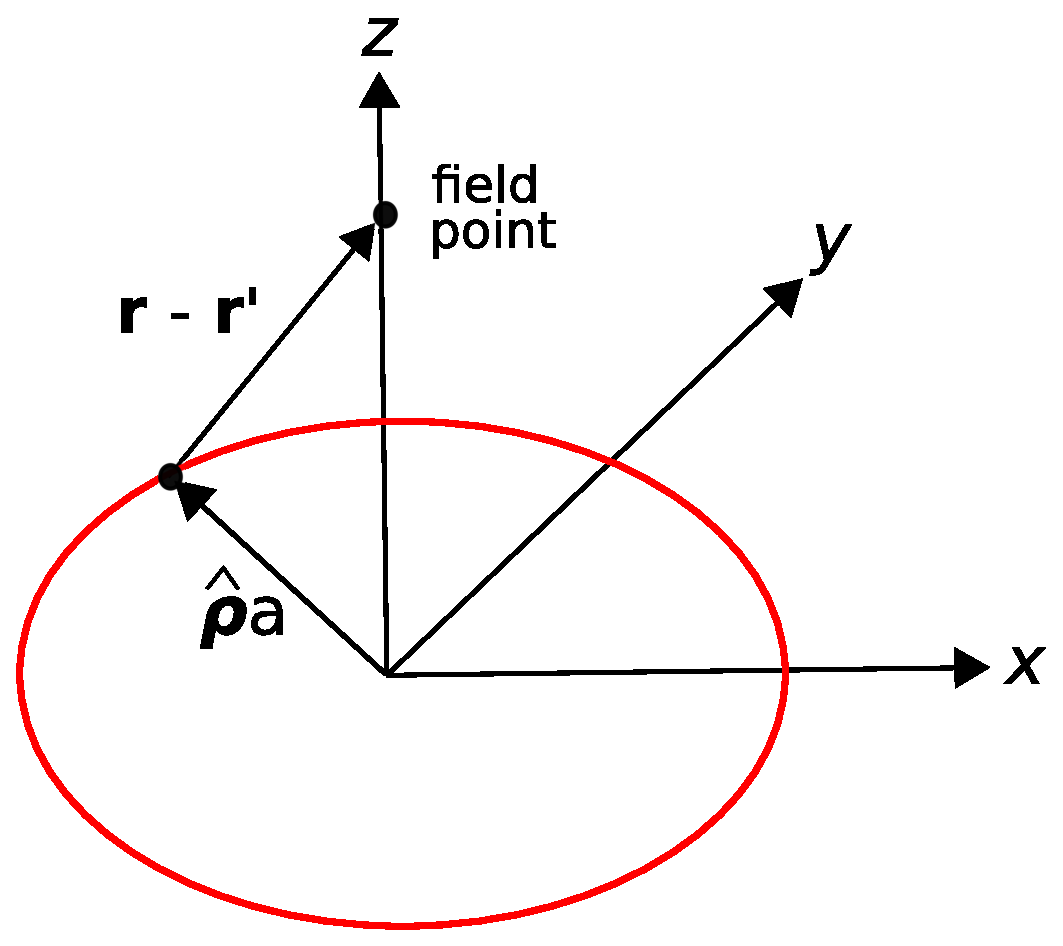
\includegraphics[width=2.5in]{modules/m0104_fRing.eps}
% https://commons.wikimedia.org/wiki/File:M0104_fRing.svg
}}{Cartesian coorinate system shown with x, y, and z axes. A red ring lies in the x and y plane, with its center at the origin. The radius of the circle is labeled bold rho hat * a. From the point at which the radius reaches the outside of the circle extends a ray labeled bold r - bold r', pointing to an arbitrary field point along the z-axis. }
\end{center} 
\centerline{\scriptsize 
\copyright~\hyperref[m0104_fRing_Credit]{K.\ Kikkeri} 
\href{https://creativecommons.org/licenses/by-sa/4.0/}{CC BY~SA 4.0} 
} 
\caption{
\label{m0104_fRing}
Calculating the electric field along the axis of a ring of charge.
}
\end{figure}
\end{example}

%---------------------------------------------------

{\bf Distribution of Charge Over a Surface.}
\index{charge density!surface}
Consider a continuous distribution of charge over a surface $\mathcal{S}$.
The surface can be divided into small patches having area $\Delta s$.  
Then, the charge associated with the $n^{\mbox{th}}$ patch, located at ${\bf r}_n$, is
%
\begin{equation}
q_n = \rho_s({\bf r}_n)~\Delta s
\end{equation}
%
where $\rho_s$ is the surface charge density (units of C/m$^2$) at ${\bf r}_n$.
Substituting this expression into Equation~\ref{m0104_eCountable}, we obtain
%
\begin{equation}
{\bf E}({\bf r}) = \frac{1}{4\pi\epsilon} \sum_{n=1}^{N} {   \frac{{\bf r}-{\bf r}_n}{\left|{\bf r}-{\bf r}_n\right|^3}~\rho_s({\bf r}_n)~\Delta s}
\end{equation}
%
Taking the limit as $\Delta s\to 0$ yields:
%
\begin{equation}
\boxed{
{\bf E}({\bf r}) = \frac{1}{4\pi\epsilon} \int_{\mathcal S} {   \frac{{\bf r}-{\bf r}'}{\left|{\bf r}-{\bf r}'\right|^3}~\rho_s({\bf r}')~ds}
}
\label{m0104_eSurfCharge}
\end{equation}
%
where ${\bf r}'$ represents the varying position over ${\mathcal S}$ with integration.

%ORB EXAMPLE
~\\ \begin{example} 
\begin{mdframed}[backgroundcolor=brown!20,linecolor=brown!20]\raggedright
Electric field along the axis of a disk of uniformly-distributed charge.
\\~\\
Consider a circular disk of radius $a$ in the $z=0$ plane, centered on the origin, as shown in Figure~\ref{m0104_fDisk}.
Let the charge density over this disk be uniform and equal to $\rho_s$ (C/m$^2$).
Find the electric field along the $z$ axis.

{\bf Solution.}
The source charge position is given in cylindrical coordinates as
%
\begin{equation}
{\bf r}' = \hat{\bf \rho}\rho  
\end{equation}
%
The position of a field point along the $z$ axis is simply
%
\begin{equation}
{\bf r} = \hat{\bf z}z  
\end{equation}
%
Thus,
%
\begin{equation}
{\bf r}-{\bf r}' = -\hat{\bf \rho}\rho + \hat{\bf z}z  
\end{equation}
%
and
%
\begin{equation}
\left|{\bf r}-{\bf r}'\right| = \sqrt{\rho^2+z^2} 
\end{equation}

Equation~\ref{m0104_eSurfCharge} becomes:
%
\begin{equation}
{\bf E}(z) = \frac{1}{4\pi\epsilon} \int_{\rho=0}^{a} \int_{\phi=0}^{2\pi} { \frac{-\hat{\bf \rho}\rho + \hat{\bf z}z}{\left[\rho^2+z^2\right]^{3/2}}~\rho_s~\left(\rho~d\rho~d\phi\right)}
\end{equation}
%
To solve this integral, first rearrange the double integral into a single integral over $\phi$ followed by integration over $\rho$:
%
\begin{equation}
\frac{\rho_s}{4\pi\epsilon} \int_{\rho=0}^{a} { \frac{\rho}{\left[\rho^2+z^2\right]^{3/2}}
                                                \left[
                                                \int_{\phi=0}^{2\pi} {
                                                                      \left(-\hat{\bf \rho}\rho + \hat{\bf z}z \right) d\phi
                                                                     }
                                                \right]
                                                d\rho      
                                              }
\label{m0104_eDisk1}
\end{equation}
%
Now we address the integration over $\phi$ shown in the square brackets in the above expression:
%
\begin{equation}
\int_{\phi=0}^{2\pi} { \left(-\hat{\bf \rho}\rho + \hat{\bf z}z \right) d\phi } 
= -\rho\int_{\phi=0}^{2\pi} { \hat{\bf \rho} d\phi } 
+ \hat{\bf z}z\int_{\phi=0}^{2\pi} { d\phi } 
\end{equation}
%
The first integral on the right is zero for the following reason.
As the integral progresses in $\phi$, the vector $\hat{\bf \rho}$ rotates.  
Because the integration is over a complete revolution (i.e., $\phi$ from 0 to $2\pi$), 
the contribution from each pointing of $\hat{\bf \rho}$ is canceled out by another pointing of $\hat{\bf \rho}$ that is in the opposite direction. 
Since there is an equal number of these canceling pairs of pointings, the result is zero.
Thus:
%
\begin{flalign}
\int_{\phi=0}^{2\pi} { \left(-\hat{\bf \rho}\rho + \hat{\bf z}z \right) d\phi }  &= 0 + \hat{\bf z}z\int_{\phi=0}^{2\pi} { d\phi } \nonumber \\
                                                                                 &= \hat{\bf z}2\pi z
\end{flalign}
%
Substituting this into Expression~\ref{m0104_eDisk1} we obtain:
%
\begin{flalign}
~&
\frac{\rho_s}{4\pi\epsilon} \int_{\rho=0}^{a} { \frac{\rho}{\left[\rho^2+z^2\right]^{3/2}}
                                                \left[
                                                \hat{\bf z}2\pi z
                                                \right]
                                                d\rho      
                                              } \nonumber \\
=& \hat{\bf z}\frac{\rho_s z}{2\epsilon} \int_{\rho=0}^{a} { \frac{\rho~d\rho}{\left[\rho^2+z^2\right]^{3/2}} }
\end{flalign}
%
This integral can be solved using integration by parts and trigonometric substitution. 
Since the solution is tedious and there is no particular principle of electromagnetics demonstrated by this solution, we shall simply state the result:
%
\begin{flalign}
\int_{\rho=0}^{a} { \frac{\rho~d\rho}{\left[\rho^2+z^2\right]^{3/2}} } &= \left.\frac{-1}{\sqrt{\rho^2+z^2}}\right|_{\rho=0}^a \nonumber \\
                                                                       &= \frac{-1}{\sqrt{a^2+z^2}} + \frac{1}{\left|z\right|}
\end{flalign}
%
Substituting this result:
%
\begin{flalign}
{\bf E}(z) &= \hat{\bf z}\frac{\rho_s z}{2\epsilon} \left( \frac{-1}{\sqrt{a^2+z^2}} + \frac{1}{\left|z\right|} \right) \nonumber \\
                 &= \hat{\bf z}\frac{\rho_s  }{2\epsilon} \left( \frac{-z}{\sqrt{a^2+z^2}} + \frac{z}{\left|z\right|} \right) \nonumber \\
                 &= \hat{\bf z}\frac{\rho_s  }{2\epsilon} \left( \frac{-z}{\sqrt{a^2+z^2}} + \mbox{sgn}~z                  \right) 
\end{flalign}
%
where ``sgn'' is the ``signum'' 
\index{signum (sgn) function}
function; i.e., $\mbox{sgn}~z =+1$ for $z>0$ and $\mbox{sgn}~z =-1$ for $z<0$.
Summarizing:
%
\begin{equation}
{\bf E}(z) = \hat{\bf z}\frac{\rho_s  }{2\epsilon} \left( \mbox{sgn}~z - \frac{z}{\sqrt{a^2+z^2}} \right)
\label{m0104_eDisk2}
\end{equation}
%
It is a good exercise to confirm that this result is dimensionally correct and yields an electric field vector that points in the expected direction  and with the expected dependence on $a$ and $z$.
%%% TODO problem to do the above
\end{mdframed}
%
\begin{figure}
\begin{center}
\pdftooltip{{  % note double braces
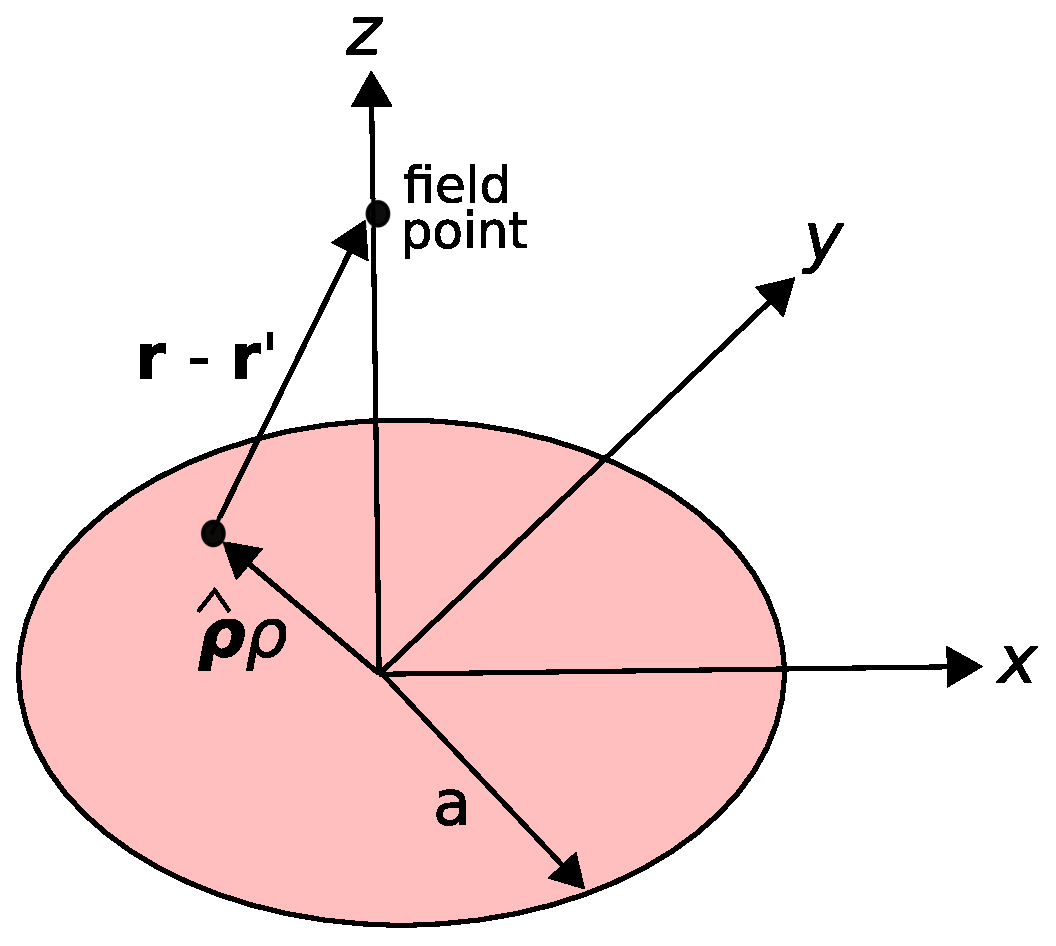
\includegraphics[width=2.5in]{modules/m0104_fDisk.eps}
% https://commons.wikimedia.org/wiki/File:M0104_fDisk.svg
}}{Cartesian coordinate system with x, y, and z axes. A red disk lies in the x-y plane, with its center at the origin and a radius (a). A ray labeled bold rho hat * rho points toward an arbitrary point in the disk. From that point, a ray labeled bold r - bold r superscript 1 points toward an arbitrary field point on the z-axis. }
\end{center} 
\centerline{\scriptsize 
\copyright~\hyperref[m0104_fDisk_Credit]{K.\ Kikkeri} 
\href{https://creativecommons.org/licenses/by-sa/4.0/}{CC BY~SA 4.0} 
} 
\caption{
\label{m0104_fDisk}
Calculating the electric field along the axis of a disk of charge.
}
\end{figure}
\end{example}


A special case of the ``disk of charge'' scenario considered in the preceding example is an \emph{infinite sheet} of charge.
The electric field from an infinite sheet of charge is a useful theoretical result.  
We get the field in this case simply by letting $a\to\infty$ in Equation~\ref{m0104_eDisk2}, yielding:
%
\begin{equation}
{\bf E}({\bf r}) = \hat{\bf z}\frac{\rho_s}{2\epsilon} \mbox{sgn}~z
\label{m0104_eISC}
\end{equation}
%
Again, it is useful to confirm that this is dimensionally correct: C/m$^2$ divided by F/m yields V/m.
Also, note that Equation~\ref{m0104_eISC} is the electric field at \emph{any} point above or below the charge sheet -- not just on $z$ axis.  This follows from symmetry.  From the perspective of any point in space, the edges of the sheet are the same distance (i.e., infinitely far) away.

%---------------------------------------------------

{\bf Distribution of Charge In a Volume.}
\index{charge density!volume}
Consider a continuous distribution of charge within a volume $\mathcal{V}$.
The volume can be divided into small cells (volume elements) having volume $\Delta v$.  
Then, the charge associated with the $n^{\mbox{th}}$ cell, located at ${\bf r}_n$, is
%
\begin{equation}
q_n = \rho_v({\bf r}_n)~\Delta v
\end{equation}
%
where $\rho_v$ is volume charge density (units of C/m$^3$) at ${\bf r}_n$.
Substituting this expression into Equation~\ref{m0104_eCountable}, we obtain
%
\begin{equation}
{\bf E}({\bf r}) = \frac{1}{4\pi\epsilon} \sum_{n=1}^{N} {   \frac{{\bf r}-{\bf r}_n}{\left|{\bf r}-{\bf r}_n\right|^3}~\rho_v({\bf r}_n)~\Delta v}
\end{equation}
%
Taking the limit as $\Delta v\to 0$ yields:
%
\begin{equation}
\boxed{
{\bf E}({\bf r}) = \frac{1}{4\pi\epsilon} \int_{\mathcal V} {   \frac{{\bf r}-{\bf r}'}{\left|{\bf r}-{\bf r}'\right|^3}~\rho_v({\bf r}')~dv}
}
\end{equation}
%
where ${\bf r}'$ represents the varying position over ${\mathcal V}$ with integration.

% %ORB EXAMPLE
% ~\\ \begin{example} 
% \begin{mdframed}[backgroundcolor=green!20] 
% Electric Field Due to a Uniform Distribution of Charge over a Cube
% \end{mdframed}
% {\color{red}NEED TO COMPLETE.}
% \centerline{\rule{2in}{1pt}} \end{example}






      \vfill\break
    \section{Gauss' Law: Integral Form}
{\color{blue}\tiny[m0014]}      % This is text associated with the open textbook "Open Electromagnetics"
% See immediately below for author, date
% This work is licensed under the Creative Commons Attribution-ShareAlike 4.0 International License. (CC BY-SA 4.0) 
% To view a copy of the license, visit http://creativecommons.org/licenses/by-sa/4.0/

%ORB TITLE Gauss' Law: Integral Form 
%ORB AUTHOR 0        # S.W. Ellingson, Virginia Tech (ellingson@vt.edu)
%ORB DATE 20180803   # yyyymmdd
%ORB ABSTRACT Gauss' Law: Integral Form 

\label{m0014_Gauss_Law_Integral_Form} % <-- Must match name of this file and module directory name.  Don't mess with this!
\index{Gauss' law!electric field|(}

Gauss' Law is one of the four fundamental laws of classical electromagnetics, collectively known as \emph{Maxwell's Equations}.
Before diving in, the reader is strongly encouraged to review Section~\ref{m0011_Electric_Flux_Density}.
In that section, Gauss' Law emerges from the interpretation of the electric field as a flux density.  
Section~\ref{m0011_Electric_Flux_Density} does not actually identify Gauss' Law, but here it is:
%
%ORB HIGHLIGHT
\begin{mdframed}[backgroundcolor=yellow!20,nobreak=true] 
\emph{Gauss' Law} (Equation~\ref{m0014_eGL}) states that the flux of the electric field through a closed surface is equal to the enclosed charge.
\end{mdframed}
%
Gauss' Law is expressed mathematically as follows:
%
\begin{equation}
\boxed{
\oint_{\mathcal S} {\bf D}\cdot d{\bf s} = Q_{encl}
}
\label{m0014_eGL}
\end{equation}
%
where 
${\bf D}$ is the electric flux density $\epsilon{\bf E}$,
${\mathcal S}$ is a closed surface with differential surface normal $d{\bf s}$, and
$Q_{encl}$ is the enclosed charge.
We can see the law is dimensionally correct;  ${\bf D}$ has units of C/m$^{2}$, thus integrating ${\bf D}$ over a surface gives a quantity with units of C/m$^{2}$ $\cdot$ m$^{2}$ = C, which are the units of charge. 
 
Gauss' Law has a number of applications in electromagnetic theory.  
One of them, as explored below, is as a method to compute the electric field in response to a distribution of electric charge.
Note that a method to do this, based on Coulomb's Law, is described in Sections~\ref{m0102_Coulombs_Law}, \ref{m0103_E_due_to_Point_Charges}, and \ref{m0104_E_due_to_a_Continuous_Distribution_of_Charge}.  
Gauss' Law provides an alternative method that is easier or more useful in certain applications.

%ORB EXAMPLE
~\\ \begin{example} 
\begin{mdframed}[backgroundcolor=brown!20,linecolor=brown!20]\raggedright
Electric field associated with a charged particle, using Gauss' Law.
\\~\\
In this example, we demonstrate the ability of Gauss' Law to predict the field associated with a charge distribution.
Let us do this for the simplest possible charge distribution. A particle of charge $q$ located at the origin, for which we already have the answer (Section~\ref{m0102_Coulombs_Law}).

{\bf Solution.}
Gauss' Law applies to {\it any} surface that encloses the charge, so for simplicity we chose a sphere of radius $r$ centered at the origin.  Note that $Q_{encl}$ on the right hand side is just $q$ for any surface having $r>0$.  Gauss' Law in this case becomes
%
\begin{equation}   
\int_{\theta=0}^{\pi} \int_{\phi=0}^{2\pi} { {\bf D} \cdot \left(\hat{\bf r}r^2 \sin\theta~d\theta~d\phi\right) } = q 
\end{equation}
%
If we can solve for ${\bf D}$, we can get ${\bf E}$ using ${\bf D} = \epsilon {\bf E}$.
The simplest way to solve for ${\bf D}$ is to use a symmetry 
\index{symmetry}
argument, which proceeds as follows. In this problem, the {\it magnitude} of ${\bf D}$ can depend only on $r$, and not $\theta$ or $\phi$. This is because the charge has no particular orientation, and the sphere is centered on the charge.  Similarly, it is clear that ${\bf D}$ must point either directly toward or directly away from the charge.  In other words, ${\bf D} = \hat{\bf r}D(r)$.  Substituting this in the above equation, we encounter the dot product $\hat{\bf r}
\cdot \hat{\bf r}$, which is simply 1.  Since $D(r)$ and $r^2$ are constants with respect to the integration, we obtain:
%
\begin{equation}   
r^2 D(r)  \int_{\theta=0}^{\pi} \int_{\phi=0}^{2\pi} { \sin\theta~d\theta d\phi } = q 
\end{equation}
%
The remaining integral is simply $4\pi$, thus we obtain:
%
\begin{equation}   
D(r)  = \frac{q}{4\pi r^2}
\end{equation}
%
Bringing the known vector orientation of ${\bf D}$ back into the equation, we obtain 
%
\begin{equation}   
{\bf D}  = \hat{\bf r}\frac{q}{4\pi r^2}
\end{equation}
%
and finally using ${\bf D} = \epsilon {\bf E}$ we obtain the expected result
%
\begin{equation}   
{\bf E}  = \hat{\bf r}\frac{q}{4\pi\epsilon r^2}
\end{equation}
\end{mdframed}\end{example}

%---------------------------------------------------------

Here's the point you should take away from the above example:
%
%ORB HIGHLIGHT
\begin{mdframed}[backgroundcolor=yellow!20,nobreak=true] 
Gauss' Law combined with a symmetry argument may be sufficient to determine the electric field due to a charge distribution.
Thus, Gauss' Law may be an easier alternative to Coulomb's Law 
\index{Coulomb's law}
in some applications.
\end{mdframed}

%-------------------------------------------------------

{\bf Additional Reading:}
\begin{itemize}
\item ``\href{https://en.wikipedia.org/wiki/Gauss'_law}{Gauss' Law}'' on Wikipedia.
\end{itemize}

\index{Gauss' law!electric field|)}

      \vfill\break
    \section{Electric Field Due to an Infinite Line Charge using Gauss' Law}
{\color{blue}\tiny[m0149]}      % This is text associated with the open textbook "Open Electromagnetics"
% See immediately below for author, date
% This work is licensed under the Creative Commons Attribution-ShareAlike 4.0 International License. (CC BY-SA 4.0) 
% To view a copy of the license, visit http://creativecommons.org/licenses/by-sa/4.0/

%ORB TITLE Electric Field Due to an Infinite Line Charge using Gauss' Law
%ORB AUTHOR 0        # S.W. Ellingson, Virginia Tech (ellingson@vt.edu)
%ORB DATE 20180803   # yyyymmdd
%ORB ABSTRACT Electric Field Due to an Infinite Line Charge using Gauss' Law

\label{m0149_E_due_to_Inf_Line_Charge} % <-- Must match name of this file and module directory name.  Don't mess with this!
\index{Gauss' law!electric field}

Section~\ref{m0014_Gauss_Law_Integral_Form} explains one application of Gauss' Law, which is to find the electric field due to a charged particle.
In this section, we present another application -- the electric field due to an infinite line of charge.
The result serves as a useful ``building block'' in a number of other problems, including determination of the capacitance of coaxial cable (Section~\ref{m0113_Capacitance_of_Coaxial_Line}).
Although this problem can be solved using the ``direct'' approach described in Section~\ref{m0104_E_due_to_a_Continuous_Distribution_of_Charge} (and it is an excellent exercise to do so), the Gauss' Law approach demonstrated here turns out to be relatively simple.

%ORB EXAMPLE
~\\ \begin{example} 
\begin{mdframed}[backgroundcolor=brown!20,linecolor=brown!20]\raggedright
Electric field associated with an infinite line charge, using Gauss' Law.
\index{charge density!line} 
\\~\\
Use Gauss' Law to determine the electric field intensity due to an infinite line of charge along the $z$ axis, having charge density $\rho_l$ (units of C/m), as shown in Figure~\ref{m0149_fGLLS}.

{\bf Solution.}
Gauss' Law requires integration over a surface that encloses the charge.
So, our first problem is to determine a suitable surface.
A cylinder of radius $a$ that is concentric with the $z$ axis, as shown in Figure~\ref{m0149_fGLLS}, is maximally symmetric with the charge distribution and so is likely to yield the simplest possible analysis.
At first glance, it seems that we may have a problem since the charge extends to infinity in the $+z$ and $-z$ directions, so it's not clear how to enclose all of the charge. 
Let's suppress that concern for a moment and simply choose a cylinder of finite length $l$.
In principle, we can solve the problem first for this cylinder of finite size, which contains only a fraction of the charge, and then later let $l\to\infty$ to capture the rest of the charge.
(In fact, we'll find when the time comes it will not be necessary to do that, but we shall prepare for it anyway.)

Here's Gauss' Law:
%
\begin{equation}
\oint_{\mathcal S} {\bf D}\cdot d{\bf s} = Q_{encl}
\label{m0149_eGL}
\end{equation}
%
where 
${\bf D}$ is the electric flux density $\epsilon{\bf E}$,
${\mathcal S}$ is a closed surface with outward-facing differential surface normal $d{\bf s}$, and
$Q_{encl}$ is the enclosed charge.

The first order of business is to constrain the form of ${\bf D}$ using a symmetry argument, 
\index{symmetry}
as follows.
Consider the field of a point charge $q$ at the origin (Section~\ref{m0014_Gauss_Law_Integral_Form}): 
%
\begin{equation}   
{\bf D}  = \hat{\bf r}\frac{q}{4\pi r^2}
\end{equation}
%
We can ``assemble'' an infinite line of charge by adding particles in pairs.
One pair is added at a time, with one particle on the $+z$ axis and the other on the $-z$ axis, with each located an equal distance from the origin. 
We continue to add particle pairs in this manner until the resulting charge extends continuously to infinity in both directions.
The principle of superposition indicates that the resulting field will be the sum of the fields of the particles (Section~\ref{m0103_E_due_to_Point_Charges}).
Thus, we see that ${\bf D}$ cannot have any component in the $\hat{\bf \phi}$ direction because none of the fields of the constituent particles have a component in that direction.
Similarly, we see that the magnitude of ${\bf D}$ cannot depend on $\phi$ because none of the fields of the constituent particles depends on $\phi$ and because the charge distribution is identical (``invariant'') with rotation in $\phi$.
Also, note that for any choice of $z$ the distribution of charge above and below that plane of constant $z$ is identical; therefore, ${\bf D}$ cannot be a function of $z$ \emph{and} ${\bf D}$  cannot have any component in the $\hat{\bf z}$ direction.
Therefore, the direction of ${\bf D}$ must be radially outward; i.e., in the $\hat{\bf \rho}$ direction, as follows:
%
\begin{equation}
{\bf D} = \hat{\bf \rho}D_{\rho}(\rho)
\end{equation}

Next, we observe that $Q_{encl}$ on the right hand side of Equation~\ref{m0149_eGL} is equal to $\rho_l l$.  Thus, we obtain
%
\begin{equation}
\oint_{\mathcal S} \left[\hat{\bf \rho}D_{\rho}(\rho)\right] \cdot d{\bf s} = \rho_l l
\end{equation}
%
The cylinder $\mathcal{S}$ consists of a flat top, curved side, and flat bottom.  Expanding the above equation to reflect this, we obtain
%
\begin{flalign}
\rho_l l =&~~~ \int_{top} \left[\hat{\bf \rho}D_{\rho}(\rho)\right] \cdot \left(+\hat{\bf z}ds\right)    \nonumber \\
          &+ \int_{side} \left[\hat{\bf \rho}D_{\rho}(\rho)\right] \cdot \left(+\hat{\bf \rho}ds\right) \nonumber \\
          &+ \int_{bottom} \left[\hat{\bf \rho}D_{\rho}(\rho)\right] \cdot \left(-\hat{\bf z}ds\right)   
\end{flalign}
%
Examination of the dot products indicates that the integrals associated with the top and bottom surfaces must be zero.  
In other words, the flux through the top and bottom is zero because ${\bf D}$ is perpendicular to these surfaces.
We are left with
%
\begin{equation}
\rho_l l = \int_{side} \left[D_{\rho}(\rho)\right] ds 
\end{equation}
%
The side surface is an open cylinder of radius $\rho=a$, so $D_{\rho}(\rho)=D_{\rho}(a)$, a constant over this surface.  Thus:
%
\begin{equation}
\rho_l l = \int_{side} \left[D_{\rho}(a)\right] ds =  \left[D_{\rho}(a)\right] \int_{side} ds 
\end{equation}
%
The remaining integral is simply the area of the side surface, which is $2\pi a \cdot l$.
Solving for $D_{\rho}(a)$ we obtain
%
\begin{equation}
D_{\rho}(a) = \frac{\rho_l l}{2\pi a l} = \frac{\rho_l}{2\pi a}
\end{equation}
%
Remarkably, we see $D_{\rho}(a)$ is independent of $l$, So the concern raised in the beginning of this solution -- that we wouldn't be able to enclose all of the charge -- doesn't matter.

Completing the solution, we note the result must be the same for any value of $\rho$ (not just $\rho=a$), so
%
\begin{equation}
{\bf D} = \hat{\rho} D_{\rho}(\rho) = \hat{\rho} \frac{\rho_l}{2\pi \rho}
\end{equation}
%
and since ${\bf D}=\epsilon{\bf E}$:
%
\begin{equation}
\boxed{
{\bf E} = \hat{\rho} \frac{\rho_l}{2\pi \epsilon \rho}
}
\end{equation}
%
This completes the solution.
We have found that the electric field is directed radially away from the line charge, and decreases in magnitude in inverse proportion to distance from the line charge. 
Suggestion: Check to ensure that this solution is dimensionally correct.
\end{mdframed}
%
\begin{figure}
\begin{center}
\pdftooltip{{  % note double braces
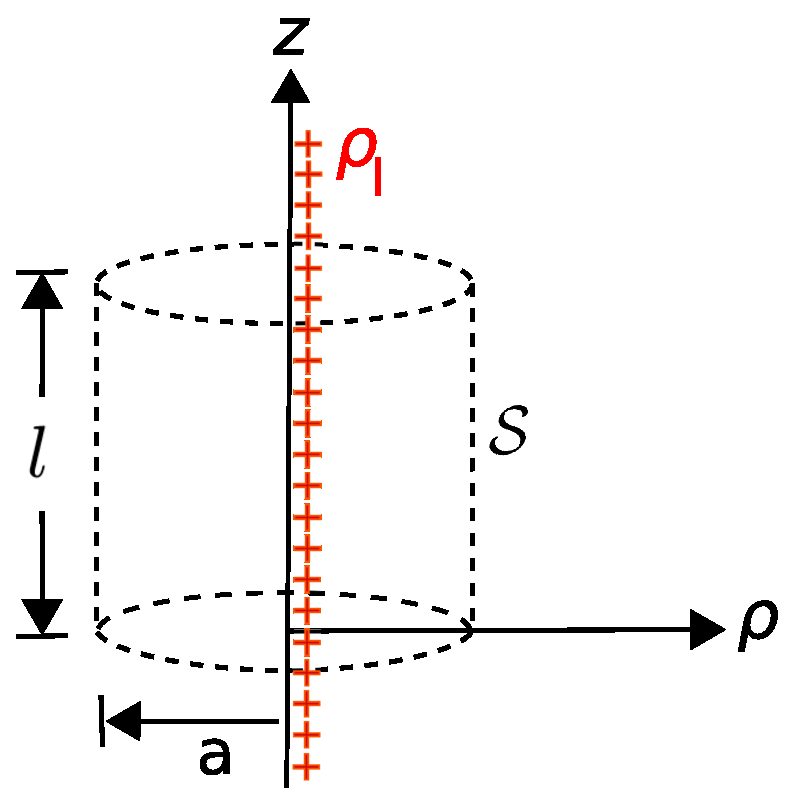
\includegraphics[width=2in]{modules/m0149_fGLLS.eps}
}}{rho and z axes are shown. A cylinder drawn with a dashed line is centered about the z axis. The lower face is positioned at the origin. Radius (a) shown from the z axis to the surface of the cylinder. Length (l) is parallel to z-axis. Positive charge is represented by orange plus signs extending to infinity in the positive and negative z direction, labeled rho sub l.}
\end{center} 
\centerline{\scriptsize 
\copyright~\hyperref[m0149_fGLLS_Credit]{K.\ Kikkeri} 
\href{https://creativecommons.org/licenses/by-sa/4.0/}{CC BY~SA 4.0} 
} 
\caption{
\label{m0149_fGLLS}
Finding the electric field of an infinite line of charge using Gauss' Law.
}
\end{figure}
\end{example}




      \vfill\break
    \section{Gauss' Law: Differential Form}
{\color{blue}\tiny[m0045]}      % This is text associated with the open textbook "Open Electromagnetics"
% See immediately below for author, date
% This work is licensed under the Creative Commons Attribution-ShareAlike 4.0 International License. (CC BY-SA 4.0) 
% To view a copy of the license, visit http://creativecommons.org/licenses/by-sa/4.0/

%ORB TITLE Gauss' Law: Differential Form
%ORB AUTHOR 0        # S.W. Ellingson, Virginia Tech (ellingson@vt.edu)
%ORB DATE 20180803   # yyyymmdd
%ORB ABSTRACT Gauss' Law: Differential Form

\label{m0045_Gauss_Law_Differential_Form_from_Integral_Form} % <-- Must match name of this file and module directory name.  Don't mess with this!
\index{Gauss' law!electric field}

The integral form of Gauss' Law (Section~\ref{m0014_Gauss_Law_Integral_Form}) is a calculation of enclosed charge $Q_{encl}$ using the surrounding density of electric flux:
%
\begin{equation}
\oint_{\mathcal S} {\bf D}\cdot d{\bf s} = Q_{encl}
\label{m0045_eGLIF}
\end{equation}
%
where ${\bf D}$ is electric flux density and ${\mathcal S}$ is the enclosing surface.
It is also sometimes necessary to do the inverse calculation (i.e., determine electric field associated with a charge distribution).
This is sometimes possible using Equation~\ref{m0045_eGLIF} if the symmetry of the problem permits; see examples in Section~\ref{m0014_Gauss_Law_Integral_Form} and \ref{m0149_E_due_to_Inf_Line_Charge}.
If the problem does not exhibit the necessary symmetry, then it seems that one must fall back to the family of techniques presented in Section~\ref{m0104_E_due_to_a_Continuous_Distribution_of_Charge} requiring direct integration over the charge, which is derived from Coulomb's Law.
\index{Coulomb's law}

However, even the Coulomb's Law / direct integration approach has a limitation that is very important to recognize: 
It does not account for the presence of structures that may influence the electric field. 
For example, the electric field due to a charge in free space is different from the electric field due to the same charge located near a perfectly-conducting surface.  
In fact, these approaches do not account for the possibility of \emph{any} spatial variation in material composition, which rules out their use in many engineering applications.

To address this broader scope of problems, we require an alternative form of Gauss' Law that applies at individual points in space.
That is, we require Gauss' Law expressed in the form of a differential equation, as opposed to an integral equation.  
This facilitates the use of Gauss' Law even in problems that do not exhibit sufficient symmetry and that involve material boundaries and spatial variations in material constitutive parameters.
Given this differential equation and the boundary conditions imposed by structure and materials, we may then solve for the electric field in these more complicated scenarios.  In this section, we derive the desired differential form of Gauss' Law.
Elsewhere (in particular, in Section~\ref{m0067_Poissons_and_Laplaces_Equations}) we use this equation as a tool to find electric fields in problems involving material boundaries.   

There are in fact two methods to develop the desired differential equation.
One method is via the definition of divergence, whereas the other is via the divergence theorem.  
Both methods are presented below because each provides a different bit of insight.  Let's explore the first method:

{\bf Derivation via the definition of divergence.}
Let the geometrical volume enclosed by ${\mathcal S}$ be ${\mathcal V}$, which has volume $V$ (units of m$^3$).  
Dividing both sides of Equation~\ref{m0045_eGLIF} by $V$ and taking the limit as $V \to 0$:
%
\begin{equation}   
\lim_{V \to 0} \frac{ \oint_{\mathcal S}{ {\bf D} \cdot d{\bf s} } }{V} = \lim_{V \to 0} \frac{ Q_{encl} }{V}
\end{equation}
%
The quantity on the right hand side is the volume charge density $\rho_v$ (units of C/m$^3$) at the point at which we converge after letting the volume go to zero.  The left hand side is, by definition, the {\it divergence} of ${\bf D}$, indicated in mathematical notation as ``$\nabla \cdot {\bf D}$'' (see Section~\ref{m0044_Divergence}). Thus, we have \emph{Gauss' Law in differential form}:
%
\begin{equation}
\boxed{
\nabla \cdot {\bf D} = \rho_v
}
\label{m0045_eGLDF}
\end{equation}
%
To interpret this equation, recall that divergence is simply the flux (in this case, {\it electric} flux) per unit volume.  

%ORB HIGHLIGHT
\begin{mdframed}[backgroundcolor=yellow!20,nobreak=true] 
Gauss' Law in differential form (Equation~\ref{m0045_eGLDF}) says that the electric flux per unit volume originating from a point in space is equal to the volume charge density at that point.
\end{mdframed}
%
%Yet another way to understand this equation: It is simply Gauss' Law in integral form (Equation~\ref{m0045_eGLIF}) applied to a vanishingly small volume.     

{\bf Derivation via the divergence theorem.}
\index{divergence theorem}
Equation~\ref{m0045_eGLDF} may also be obtained from Equation~\ref{m0045_eGLIF} using the Divergence Theorem (Section~\ref{m0046_Divergence_Theorem}), which in the present case may be written:
%
\begin{equation}
\int_{\mathcal V} \left( \nabla \cdot {\bf D} \right) dv = \oint_{\mathcal S} {\bf D}\cdot d{\bf s}
\end{equation}
%
From Equation~\ref{m0045_eGLIF}, we see that the right hand side of the equation may be replaced with the enclosed charge:
%
\begin{equation}
\int_{\mathcal V} \left( \nabla \cdot {\bf D} \right) dv = Q_{encl}
\end{equation}
%
Furthermore, the enclosed charge can be expressed as an integration of the volume charge density $\rho_v$ over ${\mathcal V}$:
%
\begin{equation}
\int_{\mathcal V} \left( \nabla \cdot {\bf D} \right) dv = \int_{\mathcal V}\rho_v dv
\end{equation}
%
The above relationship must hold regardless of the specific location or shape of ${\mathcal V}$.  The only way this is possible is if the integrands are equal.  Thus, $\nabla \cdot {\bf D}=\rho_v$, and we have obtained Equation~\ref{m0045_eGLDF}.

%ORB EXAMPLE
~\\ \begin{example} 
\begin{mdframed}[backgroundcolor=brown!20,linecolor=brown!20]\raggedright
Determining the charge density at a point, given the associated electric field.
\\~\\
The electric field intensity in free space is
%
\begin{equation}
{\bf E}({\bf r}) = \hat{\bf x}A x^2 
                 + \hat{\bf y}B z 
                 + \hat{\bf z}C x^2 z
\nonumber
\end{equation}
%
where 
$A=3~\mbox{V/m$^3$}$,
$B=2~\mbox{V/m$^2$}$, and
$C=1~\mbox{V/m$^4$}$.
What is the charge density at ${\bf r} = \hat{\bf x}2 - \hat{\bf y}2$~m?

{\bf Solution.}  First, we use ${\bf D} = \epsilon {\bf E}$ to get ${\bf D}$.  
Since the problem is in free space, $\epsilon = \epsilon_0$.  
Thus we have that the volume charge density is
%
\begin{flalign}
\rho_v &= \nabla \cdot {\bf D} \nonumber \\
       &= \nabla \cdot \left( \epsilon_0 {\bf E} \right) = \epsilon_0 \nabla \cdot {\bf E}  \nonumber \\
       &= \epsilon_0 \left[
\frac{\partial}{\partial x} \left( Ax^2 \right) +
\frac{\partial}{\partial y} \left( Bz \right) +
\frac{\partial}{\partial z} \left( C x^2 z \right)
\right] \nonumber \\
      &= \epsilon_0 \left[ 2Ax + 0 + Cx^2 \right]  \nonumber
\end{flalign} 
%
Now calculating the charge density at the specified location ${\bf r}$:
%
\begin{flalign}
& \epsilon_0 \left[ 2(3~\mbox{V/m$^3$})(2~\mbox{m}) + 0 + (1~\mbox{V/m$^4$})(2~\mbox{m})^2 \right] \nonumber \\
&= \epsilon_0\left(16~\mbox{V/m}\right) \nonumber \\
&= \mbox{142~pC/m$^3$} \nonumber 
\end{flalign} 
\end{mdframed}\end{example}

To obtain the electric field from the charge distribution in the presence of boundary conditions imposed by materials and structure, we must enforce the relevant boundary conditions.  These boundary conditions are presented in Sections~\ref{m0020_Boundary_Conditions_on_E} and \ref{m0021_Boundary_Conditions_on_D}.
Frequently, a simpler approach requiring only the boundary conditions on the electric potential ($V(\bf{r})$) is possible; this is presented in Section~\ref{m0067_Poissons_and_Laplaces_Equations}.

Furthermore, the reader should note the following. Gauss' Law does not always necessarily \emph{fully} constrain possible solutions for the electric field.  For that, we might also need Kirchoff's Voltage Law; 
\index{Kirchoff's voltage law!electrostatics}
see Section~\ref{m0152_KVL_Electrostatics_Integral-to-Differential}.

Before moving on, it is worth noting that Equation~\ref{m0045_eGLDF} can be solved in the special case in which there are no boundary conditions to satisfy; i.e., for charge only, in a uniform and unbounded medium.  In fact, no additional electromagnetic theory is required to do this. Here's the solution:
%
\begin{equation}
{\bf D}({\bf r}) = \frac{1}{4\pi} \int_{\mathcal V} {   \frac{{\bf r}-{\bf r}'}{\left|{\bf r}-{\bf r}'\right|^3}~\rho_v({\bf r}')~dv}
\end{equation}
%
which we recognize as one of the results obtained in Section~\ref{m0104_E_due_to_a_Continuous_Distribution_of_Charge} (after dividing both sides by $\epsilon$ to get ${\bf E}$).
It is reasonable to conclude that Gauss' Law (in either integral or differential form) is fundamental, whereas Coulomb's Law 
\index{Coulomb's law}
is merely a consequence of Gauss' Law.

%-------------------------------------------------------

{\bf Additional Reading:}
\begin{itemize}
\item ``\href{https://en.wikipedia.org/wiki/Gauss'_law}{Gauss' Law}'' on Wikipedia.
\item ``\href{https://en.wikipedia.org/wiki/Partial_differential_equation}{Partial differential equation}'' on Wikipedia.
\item ``\href{https://en.wikipedia.org/wiki/Boundary_value_problem}{Boundary value problem}'' on Wikipedia.
\end{itemize}

%--------------------------------

      \vfill\break
    \section{Force, Energy, and Potential Difference}
{\color{blue}\tiny[m0061]}      % This is text associated with the open textbook "Open Electromagnetics"
% See immediately below for author, date
% This work is licensed under the Creative Commons Attribution-ShareAlike 4.0 International License. (CC BY-SA 4.0) 
% To view a copy of the license, visit http://creativecommons.org/licenses/by-sa/4.0/

%ORB TITLE Force, Energy, and Potential Difference
%ORB AUTHOR 0        # S.W. Ellingson, Virginia Tech (ellingson@vt.edu)
%ORB DATE 20180806   # yyyymmdd
%ORB ABSTRACT Force, Energy, and Potential Difference

\label{m0061_Force_Energy_and_Potential_Difference} % <-- Must match name of this file and module directory name.  Don't mess with this!
\index{energy!potential|(}

The force 
\index{force}
${\bf F}_e$ experienced by a particle at location ${\bf r}$ bearing charge $q$ in an electric field intensity ${\bf E}$ is
(see Sections~\ref{m0002_Electric_Field_Intensity} and/or Section~\ref{m0102_Coulombs_Law})
%
\begin{equation}
{\bf F}_e = q {\bf E}({\bf r})
\label{m0061_eFeqE} 
\end{equation}
%
If left alone in free space, this particle would immediately begin to move.
The resulting displacement represents a loss of potential energy. 
This loss can quantified using the concept of \emph{work}, $W$.  
\index{work}
The incremental work $\Delta W$ done by moving the particle a short distance $\Delta l$, over which we assume the change in ${\bf F}_e$ is negligible, is
%
\begin{equation}
\Delta W \approx -{\bf F}_e\cdot\hat{\bf l}\Delta l
\label{m0061_WeFdl}
\end{equation}
%
where in this case $\hat{\bf l}$ is the unit vector in the direction of the motion; i.e., the direction of ${\bf F}_e$.
The minus sign indicates that potential energy of the system consisting of the electric field and the particle is being reduced. 
Like a spring that was previously compressed and is now released, the system is ``relaxing.''
   
To confirm that work defined in this way is an expression of energy, consider the units. The product of force (units of N) and distance (units of m) has units of N$\cdot$m, and 1~N$\cdot$m is 1~J of energy.

Now, what if the motion of the particle is due to factors other than the force associated with the electric field?
For example, we might consider ``resetting'' the system to it's original condition by applying an external force to overcome ${\bf F}_e$.  
Equation~\ref{m0061_WeFdl} still represents the change in potential energy of the system, but now $\hat{\bf l}$ changes sign.
The same magnitude of work is done, but now this work is positive.
In other words, positive work requires the application of an \emph{external} force that opposes and overcomes the force associated with the electric field, thereby increasing the potential energy of the system.
With respect to the analogy of a mechanical spring used above, positive work is achieved by compressing the spring.

It is also worth noting that the purpose of the dot product in Equation~\ref{m0061_WeFdl} is to ensure that only the component of motion parallel to the direction of the electric field is included in the energy tally.  This is simply because motion in any other direction cannot be due to ${\bf E}$, and therefore does not increase or decrease the associated potential energy.

We can make the relationship between work and the electric field explicit by substituting Equation~\ref{m0061_eFeqE} into Equation~\ref{m0061_WeFdl}, yielding
%
\begin{equation}
\Delta W \approx -q {\bf E}({\bf r})\cdot\hat{\bf l}\Delta l
\label{m0061_WqEdl}
\end{equation}

Equation~\ref{m0061_WqEdl} gives the work only for a short distance around ${\bf r}$.  
Now let us try to generalize this result.
If we wish to know the work done over a larger distance, then we must account for the possibility that ${\bf E}$ varies along the path taken.
To do this, we may sum contributions from points along the path traced out by the particle, i.e.,
%
\begin{equation}
W \approx \sum_{n=1}^N \Delta W ({\bf r}_n) 
\end{equation}
%
where ${\bf r}_n$ are positions defining the path.  Substituting Equation~\ref{m0061_WqEdl}, we have 
%
\begin{equation}
W \approx -q \sum_{n=1}^N {\bf E}({\bf r}_n)\cdot\hat{\bf l}({\bf r}_n)\Delta l
\end{equation}
%
Taking the limit as $\Delta l\to 0$ we obtain
%
\begin{equation}
W = -q \int_{\mathcal C} {\bf E}({\bf r})\cdot\hat{\bf l}({\bf r}) dl
\end{equation}
%
where $\mathcal{C}$ is the path (previously, the sequence of ${\bf r}_n$'s) followed.
Now omitting the explicit dependence on ${\bf r}$ in the integrand for clarity:
%
\begin{equation}
W = -q \int_{\mathcal C} {\bf E}\cdot d{\bf l}
\label{m0061_eWqint}
\end{equation}
%
where $d{\bf l} = \hat{\bf l}dl$ as usual.
Now, we are able to determine the change in potential energy for a charged particle moving along any path in space, given the electric field.

At this point, it is convenient to formally define the electric {\it potential difference} $V_{21}$ 
\index{potential difference}
between the start point (1) and end point (2) of ${\mathcal C}$.  $V_{21}$ is defined as the work done by traversing ${\mathcal C}$, per unit of charge:
%
\begin{equation}
V_{21} \triangleq \frac{W}{q} 
\end{equation}
%
This has units of J/C, which is volts (V). Substituting Equation~\ref{m0061_eWqint}, we obtain:
%
\begin{equation}
\boxed{
V_{21} = - \int_{\mathcal C} {\bf E} \cdot d{\bf l}
}
\label{m0062_eVAB}
\end{equation}
%
An advantage of analysis in terms of electrical potential as opposed to energy is that we will no longer have to explicitly state the value of the charge involved.  

%ORB HIGHLIGHT
\begin{mdframed}[backgroundcolor=yellow!20,nobreak=true] 
The potential difference $V_{21}$ between two points in space, given by Equation~\ref{m0062_eVAB}, is the change in potential energy of a charged particle divided by the charge of the particle.  Potential energy is also commonly known as ``voltage'' and has units of V. 
\end{mdframed}

%=--------------------------------

%ORB EXAMPLE
~\\ \begin{example} 
\begin{mdframed}[backgroundcolor=brown!20,linecolor=brown!20]\raggedright
Potential difference in a uniform electric field.
\\~\\
Consider an electric field ${\bf E}({\bf r}) = \hat{\bf z}E_0$, which is constant in both magnitude and direction throughout the domain of the problem. 
The path of interest is a line beginning at $\hat{\bf z}z_1$ and ending at $\hat{\bf z}z_2$.  What is $V_{21}$?
(It's worth noting that the answer to this problem is a building block for a vast number of problems in electromagnetic analysis.)

{\bf Solution.} From Equation~\ref{m0062_eVAB} we have
%
\begin{equation}
V_{21} = - \int_{z_1}^{z_2} \left( \hat{\bf z}E_0 \right) \cdot \hat{\bf z}dz = -E_0 (z_2 - z_1)
\end{equation}
%
Note $V_{21}$ is simply the electric field intensity times the distance between the points. 
This may seem familiar. For example, compare this to the findings of the battery-charged capacitor experiment described in Section~\ref{m0002_Electric_Field_Intensity}.
There too we find that potential difference equals electric field intensity times distance, and the signs agree.
\end{mdframed}\end{example}

%----------------------------------------------

The solution to the preceding example is simple because the direct path between the two points is parallel to the electric field.
If the path between the points had been \emph{perpendicular} to ${\bf E}$, then the solution is even easier -- $V_{21}$ is simply zero.  
In all other cases, $V_{21}$ is proportional to the component of the direct path between the start and end points that is parallel to ${\bf E}$, as determined by the dot product.   

\index{energy!potential|)}

      \vfill\break
    \section{Independence of Path}
{\color{blue}\tiny[m0062]}      % This is text associated with the open textbook "Open Electromagnetics"
% See immediately below for author, date
% This work is licensed under the Creative Commons Attribution-ShareAlike 4.0 International License. (CC BY-SA 4.0) 
% To view a copy of the license, visit http://creativecommons.org/licenses/by-sa/4.0/

%ORB TITLE Independence of Path
%ORB AUTHOR 0        # S.W. Ellingson, Virginia Tech (ellingson@vt.edu)
%ORB DATE 20180806   # yyyymmdd
%ORB ABSTRACT Independence of Path

\label{m0062_Independence_of_Path} % <-- Must match name of this file and module directory name.  Don't mess with this!
\index{independence of path|(}

In Section~\ref{m0061_Force_Energy_and_Potential_Difference}, we found that the potential difference (``voltage'') associated with a path ${\mathcal C}$ in an electric field intensity ${\bf E}$ is
%
\begin{equation}
V_{21} = - \int_{\mathcal C} {\bf E} \cdot d{\bf l}
\end{equation}
%
where the curve begins at point~1 and ends at point~2.
Let these points be identified using the position vectors ${\bf r}_1$ and ${\bf r}_2$, respectively.\footnote{See Section~\ref{m0006_Vector_Arithmetic} for a refresher on this concept.}
Then:
%
\begin{equation}
V_{21} = - \int_{{\bf r}_1,~\mbox{along}~\mathcal{C}}^{{\bf r}_2} {\bf E} \cdot d{\bf l}
\end{equation}
%
The associated work done by a particle bearing charge $q$ is
%
\begin{equation}
W_{21} = qV_{21}
\end{equation}
%
This work represents the change in potential energy of the system consisting of the electric field and the charged particle.  So, it must also be true that 
%
\begin{equation}
W_{21} = W_2 - W_1
\end{equation}
%
where $W_2$ and $W_1$ are the potential energies when the particle is at ${\bf r}_2$ and ${\bf r}_1$, respectively.
It is clear from the above equation that $W_{21}$ does not depend on ${\mathcal C}$; it depends only on the positions of the start and end points and not on any of the intermediate points along ${\mathcal C}$.  That is,
%
\begin{equation}
\boxed{
V_{21} = - \int_{{\bf r}_1}^{{\bf r}_2} {\bf E} \cdot d{\bf l} ~~~\mbox{, independent of}~\mathcal{C}
}
\label{m0062_eV12a}
\end{equation}
%
Since the result of the integration in Equation~\ref{m0062_eV12a} is independent of the path of integration, \emph{any} path that begins at ${\bf r}_1$ and ends at ${\bf r}_2$ yields the same value of $W_{21}$ and $V_{21}$.
We refer to this concept as \emph{independence of path}.

%ORB HIGHLIGHT
\begin{mdframed}[backgroundcolor=yellow!20,nobreak=true] 
The integral of the electric field over a path between two points depends only on the locations of the start and end points and is independent of the path taken between those points.
\end{mdframed}

A practical application of this concept is that some paths may be easier to use than others, so there may be an advantage in computing the integral in Equation~\ref{m0062_eV12a} using some path other than the path actually traversed.

\index{independence of path|)}

      \vfill\break
    \section{Kirchoff's Voltage Law for Electrostatics: Integral Form}
{\color{blue}\tiny[m0016]}      % This is text associated with the open textbook "Open Electromagnetics"
% See immediately below for author, date
% This work is licensed under the Creative Commons Attribution-ShareAlike 4.0 International License. (CC BY-SA 4.0) 
% To view a copy of the license, visit http://creativecommons.org/licenses/by-sa/4.0/

%ORB TITLE Kirchoff's Voltage Law for Electrostatics: Integral Form
%ORB AUTHOR 0        # S.W. Ellingson, Virginia Tech (ellingson@vt.edu)
%ORB DATE 20180806   # yyyymmdd
%ORB ABSTRACT Kirchoff's Voltage Law for Electrostatics (Integral Form)

\label{m0016_Kirchoffs_Voltage_Law_Electrostatics_Integral_Form} % <-- Must match name of this file and module directory name.  Don't mess with this!
\index{Kirchoff's voltage law!electrostatics|(}

As explained in Section~\ref{m0062_Independence_of_Path}, the electrical potential at point ${\bf r}_2$ relative to ${\bf r}_1$ in an electric field ${\bf E}$ (V/m) is
%
\begin{equation}
V_{21} = - \int_{{\bf r}_1}^{{\bf r}_2} {\bf E} \cdot d{\bf l}
\end{equation}
%
where the path of integration may be any path that begins and ends at the specified points.
Consider what happens if the selected path through space begins and ends at the \emph{same} point; i.e., ${\bf r}_2={\bf r}_1$.  
In this case, the path of integration is a closed loop.  
Since $V_{21}$ depends only on the positions of the start and end points and because the potential energy at those points is the same, we conclude:
% 
\begin{equation}  
\boxed{ 
\oint{ {\bf E} \cdot d{\bf l} } = 0
}
\label{m0062_eKVLES}
\end{equation}
%
This principle is known as \emph{Kirchoff's Voltage Law for Electrostatics}.

%ORB HIGHLIGHT
\begin{mdframed}[backgroundcolor=yellow!20,nobreak=true] 
Kirchoff's Voltage Law for Electrostatics (Equation~\ref{m0062_eKVLES}) states that the integral of the electric field over a closed path is zero. 
\end{mdframed}

It is worth noting that this law is a generalization of a principle of which the reader is likely already aware. 
In electric circuit theory, the sum of voltages over any closed loop in a circuit is zero.
This is also known as Kirchoff's Voltage Law because it is precisely the same principle.
To obtain Equation~\ref{m0062_eKVLES} for an electric circuit, simply partition the closed path into branches, with each branch representing one component.
Then, the integral of ${\bf E}$ over each branch is the branch voltage; i.e., units of V/m times units of m yields units of V. 
Then, the sum of these branch voltages over any closed loop is zero, as dictated by Equation~\ref{m0062_eKVLES}.

Finally, be advised that Equation~\ref{m0062_eKVLES} is specific to electrostatics.  In electrostatics, it is assumed that the electric field is independent of the magnetic field.
This is true if the magnetic field is either zero or not time-varying.  If the magnetic field is time-varying, then Equation~\ref{m0062_eKVLES} must be modified to account for the effect of the magnetic field, which is to make the right hand size potentially different from zero.  The generalized version of this expression that correctly accounts for that effect is known as the \emph{Maxwell-Faraday Equation} (Section~\ref{m0050_Maxwell-Faraday_Equation}).

%%%%%%%%%%%%%%%%%%%%%%%%%%%%%%%%%%%%

{\bf Additional Reading:}
\begin{itemize}
\item ``\href{https://en.wikipedia.org/wiki/Maxwell's_equations}{Maxwell's Equations}'' on Wikipedia.
\item ``\href{https://en.wikipedia.org/wiki/Kirchhoff's_circuit_laws}{Kirchoff's Circuit Laws}'' on Wikipedia.
\end{itemize}

\index{Kirchoff's voltage law!electrostatics|)}



      \vfill\break
    \section{Kirchoff's Voltage Law for Electrostatics: Differential Form}
{\color{blue}\tiny[m0152]}      % This is text associated with the open textbook "Open Electromagnetics"
% See immediately below for author, date
% This work is licensed under the Creative Commons Attribution-ShareAlike 4.0 International License. (CC BY-SA 4.0) 
% To view a copy of the license, visit http://creativecommons.org/licenses/by-sa/4.0/

%ORB TITLE Kirchoff's Voltage Law for Electrostatics: Differential Form 
%ORB AUTHOR 0        # S.W. Ellingson, Virginia Tech (ellingson@vt.edu)
%ORB DATE 20180806   # yyyymmdd
%ORB ABSTRACT Kirchoff's Voltage Law for Electrostatics: Differential Form 

\label{m0152_KVL_Electrostatics_Integral-to-Differential} % <-- Must match name of this file and module directory name.  Don't mess with this!
\index{Kirchoff's voltage law!electrostatics|(}

The integral form of Kirchoff's Voltage Law for electrostatics (KVL; Section~\ref{m0016_Kirchoffs_Voltage_Law_Electrostatics_Integral_Form}) states that an integral of the electric field along a closed path is equal to zero:
%
\begin{equation}
\oint_{\mathcal C}{ {\bf E} \cdot d{\bf l} } = 0  
\end{equation}
%
where ${\bf E}$ is electric field intensity and ${\mathcal C}$ is the closed curve.
In this section, we derive the differential form of this equation.
In some applications, this differential equation, combined with boundary conditions imposed by structure and materials (Sections~\ref{m0020_Boundary_Conditions_on_E} and \ref{m0021_Boundary_Conditions_on_D}), can be used to solve for the electric field in arbitrarily complicated scenarios.  
A more immediate reason for considering this differential equation is that we gain a little more insight into the behavior of the electric field, disclosed at the end of this section.

The equation we seek may be obtained using Stokes' Theorem 
\index{Stokes' theorem}
(Section~\ref{m0051_Stokes_Theorem}), which in the present case may be written:
%
\begin{equation}   
\int_{\mathcal S} \left( \nabla \times {\bf E} \right) \cdot d{\bf s} = \oint_{\mathcal C} {\bf E}\cdot d{\bf l}
\label{m0152_eKVL2}
\end{equation}
%
where ${\mathcal S}$ is any surface bounded by ${\mathcal C}$, and $d{\bf s}$ is the normal to that surface with direction determined by right-hand rule.
The integral form of KVL tells us that the right hand side of the above equation is zero, so:
%
\begin{equation}   
\int_{\mathcal S} \left( \nabla \times {\bf E} \right) \cdot d{\bf s} = 0
\end{equation}
%
The above relationship must hold regardless of the specific location or shape of ${\mathcal S}$.  The only way this is possible for all possible surfaces is if the integrand is zero at every point in space.  Thus, we obtain the desired expression:
%
\begin{equation}
\boxed{
\nabla \times {\bf E} = 0
}
\label{m0152_eKVL}
\end{equation}
% 
Summarizing:
%
%ORB HIGHLIGHT
\begin{mdframed}[backgroundcolor=yellow!20,nobreak=true] 
The differential form of Kirchoff's Voltage Law for electrostatics (Equation~\ref{m0152_eKVL}) states that the curl of the electrostatic field is zero.
\end{mdframed}

Equation~\ref{m0152_eKVL} is a partial differential equation. 
As noted above, this equation, combined with the appropriate boundary conditions, can be solved for the electric field in arbitrarily-complicated scenarios.
Interestingly, it is not the only such equation available for this purpose -- Gauss' Law (Section~\ref{m0045_Gauss_Law_Differential_Form_from_Integral_Form}) also does this.
Thus, we see a \emph{system} of partial differential equations emerging, and one may correctly infer that that the electric field is not necessarily fully constrained by either equation alone.   

%-------------------------------------------------------

{\bf Additional Reading:}
\begin{itemize}
\item ``\href{https://en.wikipedia.org/wiki/Maxwell's_equations}{Maxwell's Equations}'' on Wikipedia.
\item ``\href{https://en.wikipedia.org/wiki/Boundary_value_problem}{Boundary value problem}'' on Wikipedia.
\end{itemize}

\index{Kirchoff's voltage law!electrostatics|)}


      \vfill\break
    \section{Electric Potential Field Due to Point Charges}
{\color{blue}\tiny[m0064]}      % This is text associated with the open textbook "Open Electromagnetics"
% See immediately below for author, date
% This work is licensed under the Creative Commons Attribution-ShareAlike 4.0 International License. (CC BY-SA 4.0) 
% To view a copy of the license, visit http://creativecommons.org/licenses/by-sa/4.0/

%ORB TITLE Electric Potential Field Due to Point Charges
%ORB AUTHOR 0        # S.W. Ellingson, Virginia Tech (ellingson@vt.edu)
%ORB DATE 20180806   # yyyymmdd
%ORB ABSTRACT Electric Potential due to Point Charges

\label{m0064_V_due_to_Point_Charges} % <-- Must match name of this file and module directory name.  Don't mess with this!

The electric field intensity due to a point charge $q$ at the origin is
(see Section~\ref{m0102_Coulombs_Law} or \ref{m0014_Gauss_Law_Integral_Form}) 
%
\begin{equation}   
{\bf E}  = \hat{\bf r}\frac{q}{4\pi\epsilon r^2}
\label{eEPPCE}
\end{equation}
%
In Sections~\ref{m0061_Force_Energy_and_Potential_Difference} and \ref{m0062_Independence_of_Path}, it was determined that the potential difference measured from position ${\bf r}_1$ to position ${\bf r}_2$ is
%
\begin{equation}
V_{21} = - \int_{{\bf r}_1}^{{\bf r}_2} {\bf E} \cdot d{\bf l}
\label{m0064_eV12}
\end{equation}

This method for calculating potential difference is often a bit awkward.  
To see why, consider an example from circuit theory, shown in Figure~\ref{m0064_fResistor}.
In this example, consisting of a single resistor and a ground node, we've identified four quantities:
%
\begin{itemize}
\item The resistance $R$
\item The current $I$ through the resistor
\item The node voltage $V_1$, which is the potential difference measured from ground to the left side of the resistor 
\item The node voltage $V_2$, which is the potential difference measured from ground to the right side of the resistor
\end{itemize}
%
Let's say we wish to calculate the potential difference $V_{21}$ across the resistor.
There are two ways this can be done:
%
\begin{itemize}
\item $V_{21}=-IR$  
\item $V_{21}=V_2-V_1$
\end{itemize}
%
The advantage of the second method is that it is not necessary to know $I$, $R$, or indeed anything about what is happening between the nodes; it is only necessary to know the node voltages.
The point is that it is often convenient to have a common \emph{datum} 
\index{datum}
-- in this example, ground 
\index{ground}
-- with respect to which the potential differences at all other locations of interest can be defined.  When we have this, calculating potential differences reduced to simply subtracting predetermined node potentials.
%
\begin{figure}
\begin{center}
\pdftooltip{{  % note double braces
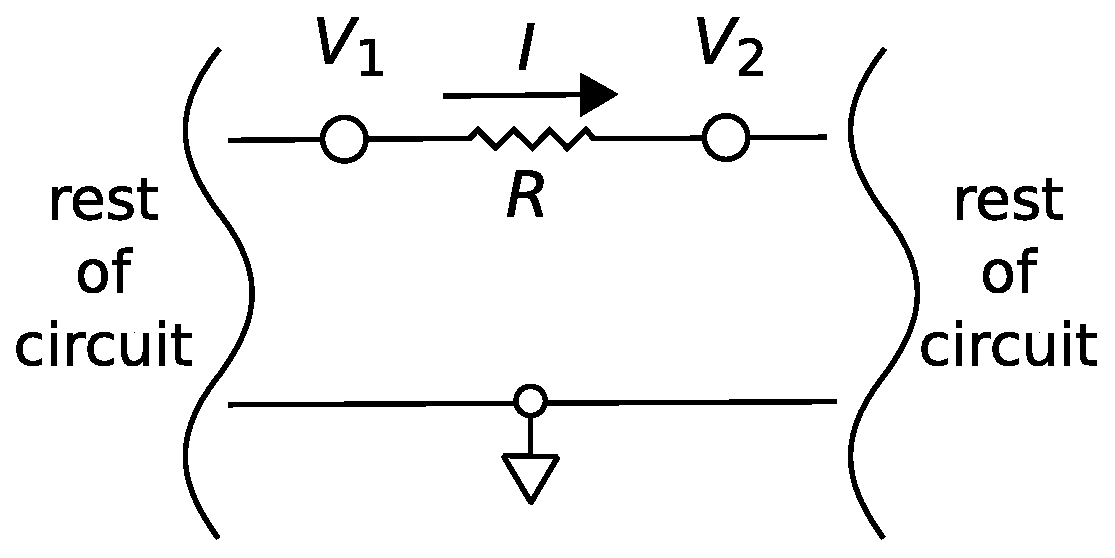
\includegraphics[width=2.5in]{modules/m0064_fResistor.eps}
% https://commons.wikimedia.org/wiki/File:M0064_fResistor.svg
}}{The diagram shows part of a circuit. Two curved lines on the left and right side of the figure indicate where the rest of the circuit is. The top branch has two nodes, labeled V sub 1 and V sub 2. Between them is a resistor (R), with an arrow pointed to the right to indicate the path of the current. On the bottom branch is a symbol for ground. }
\end{center} 
\centerline{\scriptsize 
\copyright~\hyperref[m0064_fResistor_Credit]{K.\ Kikkeri} 
\href{https://creativecommons.org/licenses/by-sa/4.0/}{CC BY~SA 4.0} 
} 
\caption{
\label{m0064_fResistor}
A resistor in a larger circuit, used as an example to demonstrate the concept of node voltages. 
}
\end{figure}

So, can we establish a datum in general electrostatic problems that works the same way?
The answer is yes.
The datum is arbitrarily chosen to be a sphere that encompasses the universe; i.e., a sphere with radius $\to\infty$.
Employing this choice of datum, we can use Equation~\ref{m0064_eV12} to define $V({\bf r})$, the potential at point ${\bf r}$, as follows:
%
\begin{equation}
\boxed{
V({\bf r}) \triangleq - \int_{\infty}^{{\bf r}} {\bf E} \cdot d{\bf l}
}
\label{m0064_eVP}
\end{equation}

%ORB HIGHLIGHT
\begin{mdframed}[backgroundcolor=yellow!20,nobreak=true] 
The electrical potential at a point, given by Equation~\ref{m0064_eVP}, is defined as the potential difference measured beginning at a sphere of infinite radius and ending at the point ${\bf r}$.  The potential obtained in this manner is with respect to the potential infinitely far away.
\end{mdframed}

In the particular case where ${\bf E}$ is due to the point charge at the origin:
%
\begin{equation}
V({\bf r}) = - \int_{\infty}^{{\bf r}} \left[ \hat{\bf r}\frac{q}{4\pi\epsilon r^2}  \right] \cdot d{\bf l}
\end{equation}
%
The principle of \emph{independence of path} (Section~\ref{m0062_Independence_of_Path}) asserts that the path of integration doesn't matter as long as the path begins at the datum at infinity and ends at ${\bf r}$. 
So, we should choose the easiest such path.
The radial symmetry of the problem indicates that the easiest path will be a line of constant $\theta$ and $\phi$, so we choose $d{\bf l}=\hat{\bf r}dr$.
Continuing:
%
\begin{flalign}
V({\bf r}) &= - \int_{\infty}^{r} \left[ \hat{\bf r}\frac{q}{4\pi\epsilon r^2}  \right] \cdot \left[ \hat{\bf r}dr \right] \\
           &= - \frac{q}{4\pi\epsilon} \int_{\infty}^{r} \frac{1}{r^2} dr \\
           &= + \frac{q}{4\pi\epsilon} \left.\frac{1}{r}\right|^{r}_{\infty} %= \left(-\frac{q}{4\pi\epsilon r}\right) - 0
\end{flalign}
%
so
%
\begin{equation}
\boxed{
V({\bf r}) = + \frac{q}{4\pi\epsilon r}
}
\label{m0064_eV}
\end{equation}
%
(Suggestion: Confirm that Equation~\ref{m0064_eV} is dimensionally correct.)
In the context of the circuit theory example above, this is the ``node voltage'' at ${\bf r}$ when the datum is defined to be the surface of a sphere at infinity.
Subsequently, we may calculate the potential difference from any point ${\bf r}_1$ to any other point ${\bf r}_2$ as
%
\begin{equation}
V_{21} = V({\bf r}_2)-V({\bf r}_1)
\end{equation}
%
and that will typically be a \emph{lot} easier than using Equation~\ref{m0064_eV12}.

It is not often that one deals with systems consisting of a single charged particle.
So, for the above technique to be truly useful, we need a straightforward way to determine the potential field $V({\bf r})$ for arbitrary distributions of charge.
The first step in developing a more general expression is to determine the result for a particle located at a point ${\bf r}'$ somewhere other than the origin.
Since Equation~\ref{m0064_eV} depends only on charge and the distance between the field point ${\bf r}$ and ${\bf r}'$, we have
%
\begin{equation}
V({\bf r};{\bf r}') \triangleq + \frac{q'}{4\pi\epsilon \left|{\bf r}-{\bf r}'\right|}
\label{m0064_eVd}
\end{equation}
%
where, for notational consistency, we use the symbol $q'$ to indicate the charge.
Now applying superposition, the potential field due to $N$ charges is
%
\begin{equation}
V({\bf r}) = \sum_{n=1}^N { V({\bf r};{\bf r}_n) }
\end{equation}
%
Substituting Equation~\ref{m0064_eVd} we obtain:
%
\begin{equation}
\boxed{
V({\bf r}) = \frac{1}{4\pi\epsilon} \sum_{n=1}^N { \frac{q_n}{\left|{\bf r}-{\bf r}_n\right|} }
}
\label{m0064_eVN}
\end{equation}
%
%ORB HIGHLIGHT
\begin{mdframed}[backgroundcolor=yellow!20,nobreak=true] 
Equation~\ref{m0064_eVN} gives the electric potential at a specified location due to a finite number of charged particles.
\end{mdframed}
%
The potential field due to continuous distributions of charge is addressed in Section~\ref{m0065_V_due_to_a_Continuous_Distribution_of_Charge}. 



      \vfill\break
    \section{Electric Potential Field due to a Continuous Distribution of Charge}
{\color{blue}\tiny[m0065]}      % This is text associated with the open textbook "Open Electromagnetics"
% See immediately below for author, date
% This work is licensed under the Creative Commons Attribution-ShareAlike 4.0 International License. (CC BY-SA 4.0) 
% To view a copy of the license, visit http://creativecommons.org/licenses/by-sa/4.0/

%ORB TITLE Electric Potential Field due to a Continuous Distribution of Charge
%ORB AUTHOR 0        # S.W. Ellingson, Virginia Tech (ellingson@vt.edu)
%ORB DATE 20180806   # yyyymmdd
%ORB ABSTRACT Electric Potential due to a Continuous Distribution of Charge

\label{m0065_V_due_to_a_Continuous_Distribution_of_Charge} % <-- Must match name of this file and module directory name.  Don't mess with this!

The electrostatic potential field at ${\bf r}$ associated with $N$ charged particles is
%
\begin{equation}
V({\bf r}) = \frac{1}{4\pi\epsilon} \sum_{n=1}^N { \frac{q_n}{\left|{\bf r}-{\bf r}_n\right|} }
\label{m0065_eCountable}
\end{equation}
%
where $q_n$ and ${\bf r_n}$ are the charge and position of the $n^{\mbox{th}}$ particle.
However, it is more common to have a continuous distribution of charge as opposed to a countable number of charged particles.
We now consider how to compute $V({\bf r})$ three types of these commonly-encountered distributions.
Before beginning, it's worth noting that the methods will be essentially the same, from a mathematical viewpoint, as those developed in Section~\ref{m0104_E_due_to_a_Continuous_Distribution_of_Charge}; therefore, a review of that section may be helpful before attempting this section.

%---------------------------------------------------

{\bf Continuous Distribution of Charge Along a Curve.}
\index{charge density!line}
Consider a continuous distribution of charge along a curve $\mathcal{C}$.
The curve can be divided into short segments of length $\Delta l$.  
Then, the charge associated with the $n^{\mbox{th}}$ segment, located at ${\bf r}_n$, is
%
\begin{equation}
q_n = \rho_l({\bf r}_n)~\Delta l
\end{equation}
%
where $\rho_l$ is the line charge density (units of C/m) at ${\bf r}_n$.
Substituting this expression into Equation~\ref{m0065_eCountable}, we obtain
%
\begin{equation}
{\bf V}({\bf r}) = \frac{1}{4\pi\epsilon} \sum_{n=1}^{N} { \frac{\rho_l({\bf r}_n)}{\left|{\bf r}-{\bf r}_n\right|} \Delta l}
\end{equation}
%
Taking the limit as $\Delta l\to 0$ yields:
%
\begin{equation}
V({\bf r}) = \frac{1}{4\pi\epsilon} \int_{\mathcal C} { \frac{\rho_l(l)}{\left|{\bf r}-{\bf r}'\right|} dl}
\label{m0065_eLineCharge}
\end{equation}
%
where ${\bf r}'$ represents the varying position along ${\mathcal C}$ with integration along the length $l$.


%---------------------------------------------------

{\bf Continuous Distribution of Charge Over a Surface.}
\index{charge density!surface}
Consider a continuous distribution of charge over a surface $\mathcal{S}$.
The surface can be divided into small patches having area $\Delta s$.  
Then, the charge associated with the $n^{\mbox{th}}$ patch, located at ${\bf r}_n$, is
%
\begin{equation}
q_n = \rho_s({\bf r}_n)~\Delta s
\end{equation}
%
where $\rho_s$ is surface charge density (units of C/m$^2$) at ${\bf r}_n$.
Substituting this expression into Equation~\ref{m0065_eCountable}, we obtain
%
\begin{equation}
V({\bf r}) = \frac{1}{4\pi\epsilon} \sum_{n=1}^{N} { \frac{\rho_s({\bf r}_n)}{\left|{\bf r}-{\bf r}_n\right|}~\Delta s}
\end{equation}
%
Taking the limit as $\Delta s\to 0$ yields:
%
\begin{equation}
V({\bf r}) = \frac{1}{4\pi\epsilon} \int_{\mathcal S} { \frac{\rho_s({\bf r}')}{\left|{\bf r}-{\bf r}'\right|}~ds}
\label{m0065_eSurfCharge}
\end{equation}
%
where ${\bf r}'$ represents the varying position over ${\mathcal S}$ with integration.

%---------------------------------------------------

{\bf Continuous Distribution of Charge in a Volume.}
\index{charge density!volume}
Consider a continuous distribution of charge within a volume $\mathcal{V}$.
The volume can be divided into small cells (volume elements) having area $\Delta v$.  
Then, the charge associated with the $n^{\mbox{th}}$ cell, located at ${\bf r}_n$, is
%
\begin{equation}
q_n = \rho_v({\bf r}_n)~\Delta v
\end{equation}
%
where $\rho_v$ is the volume charge density (units of C/m$^3$) at ${\bf r}_n$.
Substituting this expression into Equation~\ref{m0065_eCountable}, we obtain
%
\begin{equation}
V({\bf r}) = \frac{1}{4\pi\epsilon} \sum_{n=1}^{N} {   \frac{\rho_v({\bf r}_n)}{\left|{\bf r}-{\bf r}_n\right|}~\Delta v}
\end{equation}
%
Taking the limit as $\Delta v\to 0$ yields:
%
\begin{equation}
V({\bf r}) = \frac{1}{4\pi\epsilon} \int_{\mathcal V} {   \frac{\rho_v({\bf r}')}{\left|{\bf r}-{\bf r}'\right|}~dv}
\end{equation}
%
where ${\bf r}'$ represents the varying position over ${\mathcal V}$ with integration.



      \vfill\break
    \section{Electric Field as the Gradient of Potential}
{\color{blue}\tiny[m0063]}      % This is text associated with the open textbook "Open Electromagnetics"
% See immediately below for author, date
% This work is licensed under the Creative Commons Attribution-ShareAlike 4.0 International License. (CC BY-SA 4.0) 
% To view a copy of the license, visit http://creativecommons.org/licenses/by-sa/4.0/

%ORB TITLE Electric Field as the Gradient of Potential
%ORB AUTHOR 0        # S.W. Ellingson, Virginia Tech (ellingson@vt.edu)
%ORB DATE 20180806   # yyyymmdd
%ORB ABSTRACT Electric Field as the Gradient of Potential

\label{m0063_Electric_Field_as_the_Gradient_of_Potential} % <-- Must match name of this file and module directory name.  Don't mess with this!

In Section~\ref{m0061_Force_Energy_and_Potential_Difference}, it was determined that the electrical potential difference $V_{21}$ measured over a path ${\mathcal C}$ is given by 
%
\begin{equation}
V_{21} = - \int_{\mathcal C} {\bf E}({\bf r}) \cdot d{\bf l}
\label{m0063_eV12}
\end{equation}
%
where ${\bf E}({\bf r})$ is the electric field intensity at each point ${\bf r}$ along ${\mathcal C}$.
In Section~\ref{m0064_V_due_to_Point_Charges}, we defined the scalar electric potential field $V({\bf r})$ as the electric potential difference at ${\bf r}$ relative to a datum at infinity.
In this section, we address the ``inverse problem'' -- namely, how to calculate ${\bf E}({\bf r})$ given $V({\bf r})$.
Specifically, we are interested in a direct ``point-wise'' mathematical transform from one to the other.
Since Equation~\ref{m0063_eV12} is in the form of an integral, it should not come as a surprise that the desired expression will be in the form of a differential equation.

We begin by identifying the contribution of an infinitesimal length of the integral to the total integral in Equation~\ref{m0063_eV12}.  At point ${\bf r}$, this is
%
\begin{equation}
dV = - {\bf E}({\bf r}) \cdot d{\bf l}
\label{eVABd}
\end{equation}
%
Although we can proceed using any coordinate system, the following derivation is particularly simple in Cartesian coordinates.  In Cartesian coordinates,
%
\begin{equation}
d{\bf l} = \hat{\bf x}dx + \hat{\bf y}dy + \hat{\bf z}dz
\end{equation}
%
We also note that for any scalar function of position, including $V({\bf r})$, it is true that
%
\begin{equation}
dV = \frac{\partial V}{\partial x} dx + \frac{\partial V}{\partial y} dy + \frac{\partial V}{\partial z} dz 
\end{equation}
%
Note the above relationship is not specific to electromagnetics; it is simply mathematics.  
Also note that $dx = d{\bf l} \cdot \hat{\bf x}$ and so on for $dy$ and $dz$.  
Making these substitutions into the above equation, we obtain:
%
\begin{equation}
dV = \frac{\partial V}{\partial x} \left( d{\bf l} \cdot \hat{\bf x} \right) 
+ \frac{\partial V}{\partial y} \left( d{\bf l} \cdot \hat{\bf y} \right)
+ \frac{\partial V}{\partial z} \left( d{\bf l} \cdot \hat{\bf z} \right)
\end{equation}
%
This equation may be rearranged as follows:
%
\begin{equation}
dV =  
\left( 
\left[ \hat{\bf x}  \frac{\partial}{\partial x} 
+ \hat{\bf y} \frac{\partial}{\partial y} 
+ \hat{\bf z}\frac{\partial}{\partial z}  \right] V
\right) \cdot d{\bf l}
\end{equation}
%
Comparing the above equation to Equation~\ref{eVABd}, we find:
%
\begin{equation}
{\bf E}({\bf r}) = - \left[ \hat{\bf x}\frac{\partial}{\partial x}   
+ \hat{\bf y} \frac{\partial}{\partial y} 
+ \hat{\bf z}\frac{\partial}{\partial z}  \right] V
\end{equation}
%
Note that the quantity in square brackets is the gradient 
\index{gradient}
operator ``$\nabla$'' (Section~\ref{m0098_Gradient}).
Thus, we may write
%
\begin{equation}
\boxed{
{\bf E} = - \nabla V
}
\label{m0063_eEPEDV}
\end{equation}
%
which is the relationship we seek.

%ORB HIGHLIGHT
\begin{mdframed}[backgroundcolor=yellow!20,nobreak=true] 
The electric field intensity at a point is the gradient of the electric potential at that point after a change of sign (Equation~\ref{m0063_eEPEDV}).
\end{mdframed}

Using Equation~\ref{m0063_eEPEDV}, we can immediately find the electric field at any point ${\bf r}$ if we can describe $V$ as a function of ${\bf r}$.  
Furthermore, this relationship between $V$ and ${\bf E}$ has a useful physical interpretation.
Recall that the gradient of a scalar field is a vector that points in the direction in which that field increases most quickly. 
Therefore:
%
%ORB HIGHLIGHT
\begin{mdframed}[backgroundcolor=yellow!20,nobreak=true] 
The electric field points in the direction in which the electric potential most rapidly decreases.
\end{mdframed}
%
This result should not come as a complete surprise; for example, the reader should already be aware that the electric field points away from regions of net positive charge and toward regions of net negative charge (Sections~\ref{m0002_Electric_Field_Intensity} and/or \ref{m0102_Coulombs_Law}).
What is new here is that both the magnitude and direction of the electric field may be determined given only the potential field, without having to consider the charge that is the physical source of the electrostatic field.

%%%%%%%%%%%%%%%%%%%%%%%%%%%%%%%%%%%%%%%%%%%%%%%%%

%ORB EXAMPLE
~\\ \begin{example} 
\begin{mdframed}[backgroundcolor=brown!20,linecolor=brown!20]\raggedright
Electric field of a charged particle, beginning with the potential field. 
\\~\\
In this example, we determine the electric field of a particle bearing charge $q$ located at the origin. 
This may be done in a ``direct'' fashion using Coulomb's Law (Section~\ref{m0102_Coulombs_Law}).
However, here we have the opportunity to find the electric field using a different method.
In Section~\ref{m0064_V_due_to_Point_Charges} we found the scalar potential for this source was:
%
\begin{equation}
V({\bf r}) = \frac{q}{4\pi\epsilon r}
\end{equation}
%
So, we may obtain the electric field using Equation~\ref{m0063_eEPEDV}:
%
\begin{equation}
{\bf E} = - \nabla V = -\nabla \left( \frac{q}{4\pi\epsilon r} \right)
\end{equation}
%
Here $V({\bf r})$ is expressed in spherical coordinates, so we have (Section~\ref{m0139_Vector_Operators}):
%
\begin{equation}
{\bf E} = -\left[ \hat{\bf r}\frac{\partial}{\partial r}
+\hat{\bf \theta}\frac{1}{r}\frac{\partial}{\partial \theta}
+\hat{\bf \phi}\frac{1}{r\sin\theta}\frac{\partial}{\partial \phi} 
 \right] \left( \frac{q}{4\pi\epsilon r} \right)
\end{equation}
%
In this case, $V({\bf r})$ does not vary with $\phi$ or $\theta$, so the second and third terms of the gradient are zero.
This leaves
%
\begin{flalign}
{\bf E} &= -\hat{\bf r}\frac{\partial}{\partial r}\left( \frac{q}{4\pi\epsilon r} \right) \nonumber \\
        &= -\hat{\bf r} \frac{q}{4\pi\epsilon} \frac{\partial}{\partial r} \frac{1}{r} \nonumber \\
        &= -\hat{\bf r} \frac{q}{4\pi\epsilon} \left( -\frac{1}{r^2} \right) 
\end{flalign}
%
So we find 
%
\begin{flalign}
{\bf E} = +\hat{\bf r} \frac{q}{4\pi\epsilon r^2} 
\end{flalign}
%
as was determined in Section~\ref{m0102_Coulombs_Law}.
\end{mdframed}\end{example}


      \vfill\break
    \section{Poisson's and Laplace's Equations}
{\color{blue}\tiny[m0067]}      % This is text associated with the open textbook "Open Electromagnetics"
% See immediately below for author, date
% This work is licensed under the Creative Commons Attribution-ShareAlike 4.0 International License. (CC BY-SA 4.0) 
% To view a copy of the license, visit http://creativecommons.org/licenses/by-sa/4.0/

%ORB TITLE Poisson's and Laplace's Equations
%ORB AUTHOR 0        # S.W. Ellingson, Virginia Tech (ellingson@vt.edu)
%ORB DATE 20180806   # yyyymmdd
%ORB ABSTRACT Poisson's and Laplace's Equations

\label{m0067_Poissons_and_Laplaces_Equations} % <-- Must match name of this file and module directory name.  Don't mess with this!
\index{Poisson's equation|(}

The electric scalar potential field $V({\bf r})$, defined in Section~\ref{m0064_V_due_to_Point_Charges}, is useful for a number of reasons including 
the ability to conveniently compute potential differences
(i.e., $V_{21} = V({\bf r}_2) - V({\bf r}_1)$)
and the ability to conveniently determine the electric field by taking the gradient
(i.e., ${\bf E}=-\nabla V$).  
One way to obtain $V({\bf r})$ is by integration over the source charge distribution, as described in Section~\ref{m0065_V_due_to_a_Continuous_Distribution_of_Charge}.
This method is awkward in the presence of material interfaces, which impose boundary conditions on the solutions that must be satisfied simultaneously.  
For example, the electric potential on a perfectly conducting surface is constant\footnote{This fact is probably already known to the reader from past study of elementary circuit theory; however, this is established in the context of electromagnetics in Section~\ref{m0025_Charge_and_Electric_Field_for_a_Perfectly_Conducting_Region}.} 
-- a constraint which is not taken into account in any of the expressions in Section~\ref{m0065_V_due_to_a_Continuous_Distribution_of_Charge}.

In this section, we develop an alternative approach to calculating $V({\bf r})$ that accommodates these boundary conditions, and thereby facilitates the analysis of the scalar potential field in the vicinity of structures and spatially-varying material properties.
This alternative approach is based on \emph{Poisson's Equation}, which we now derive. 

We begin with the differential form of Gauss' Law (Section~\ref{m0045_Gauss_Law_Differential_Form_from_Integral_Form}):
%
\begin{equation}
\nabla \cdot {\bf D} = \rho_v
\end{equation}
%
Using the relationship ${\bf D}=\epsilon{\bf E}$ (and keeping in mind our standard assumptions about material properties, summarized in Section~\ref{m0007_Properties_of_Materials}) we obtain
%
\begin{equation}
\nabla \cdot {\bf E} = \frac{\rho_v}{\epsilon}
\end{equation}
%
Next, we apply the relationship (Section~\ref{m0063_Electric_Field_as_the_Gradient_of_Potential}):
%
\begin{equation}
{\bf E} = -\nabla V
\end{equation}
%
yielding
%
\begin{equation}
\nabla \cdot \nabla V = - \frac{\rho_v}{\epsilon}
\end{equation}
%
This is Poisson's Equation, but it is not in the form in which it is commonly employed.  
To obtain the alternative form, consider the operator $\nabla \cdot \nabla$ in Cartesian coordinates:
%
\begin{flalign}
\nabla \cdot \nabla &= 
\left[ \frac{\partial}{\partial x} \hat{\bf x}  
+ \frac{\partial}{\partial y} \hat{\bf y} 
+ \frac{\partial}{\partial z} \hat{\bf z} \right]
\cdot
\left[ \frac{\partial}{\partial x} \hat{\bf x}  
+ \frac{\partial}{\partial y} \hat{\bf y} 
+ \frac{\partial}{\partial z} \hat{\bf z} \right] \nonumber \\
 &= 
\frac{\partial^2}{\partial x^2}  
+ \frac{\partial^2}{\partial y^2}  
+ \frac{\partial^2}{\partial z^2}  \nonumber \\
 &= \nabla^2 
\end{flalign}
%
i.e., the operator $\nabla \cdot \nabla$ is identically the Laplacian operator $\nabla^2$ (Section~\ref{m0099_The_Laplacian_Operator}).
Furthermore, this is true regardless of the coordinate system employed.  
Thus, we obtain the following form of Poisson's Equation:
%
\begin{equation}
\boxed{
\nabla^2 V = - \frac{\rho_v}{\epsilon}
}
\label{m0067_ePoisson}
\end{equation}

%ORB HIGHLIGHT
\begin{mdframed}[backgroundcolor=yellow!20,nobreak=true] 
Poisson's Equation (Equation~\ref{m0067_ePoisson}) states that the Laplacian of the electric potential field is equal to the volume charge density divided by the permittivity, with a change of sign. 
\end{mdframed}

Note that Poisson's Equation is a partial differential equation, and therefore can be solved using well-known techniques already established for such equations.
In fact, Poisson's Equation is an \emph{inhomogeneous} differential equation, with the inhomogeneous part $-\rho_v/\epsilon$ representing the source of the field.  
In the presence of material structure, we identify the relevant boundary conditions at the interfaces between materials, and the task of finding $V({\bf r})$ is reduced to the purely mathematical task of solving the associated boundary value problem (see ``Additional Reading'' at the end of this section).  This approach is particularly effective when one of the materials is a perfect conductor or can be modeled as such a material.
This is because -- as noted at the beginning of this section -- the electric potential at all points on the surface of a perfect conductor must be equal, resulting in a particularly simple boundary condition.  
  
In many other applications, the charge responsible for the electric field lies outside the domain of the problem; i.e., we have non-zero electric field (hence, potentially non-zero electric potential) in a region that is free of charge.  In this case, Poisson's Equation simplifies to \emph{Laplace's Equation}: 
\index{Laplace's equation}
%
\begin{equation}
\boxed{
\nabla^2 V = 0 ~~\mbox{(source-free region)}
}
\label{m0067_eLaplace}
\end{equation}
%
%ORB HIGHLIGHT
\begin{mdframed}[backgroundcolor=yellow!20,nobreak=true] 
Laplace's Equation (Equation~\ref{m0067_eLaplace}) states that the Laplacian of the electric potential field is zero in a source-free region. 
\end{mdframed}
%
Like Poisson's Equation, Laplace's Equation, combined with the relevant boundary conditions, can be used to solve for $V({\bf r})$, but only in regions that contain no charge.

%%%%%%%%%%%%%%%%%%%%%%%%%%%%%%%%%%%%%%%%%%%%%%%%%%%%%%%%%%%%%%%

{\bf Additional Reading:}
\begin{itemize}
\item ``\href{https://en.wikipedia.org/wiki/Poisson's_equation}{Poisson's equation}'' on Wikipedia.
\item ``\href{https://en.wikipedia.org/wiki/Boundary_value_problem}{Boundary value problem}'' on Wikipedia.
\item ``\href{https://en.wikipedia.org/wiki/Laplace's_equation}{Laplace's equation}'' on Wikipedia.
\end{itemize}

\index{Poisson's equation|)}




      \vfill\break
    \section{Potential Field Within a Parallel Plate Capacitor}
{\color{blue}\tiny[m0068]}      % This is text associated with the open textbook "Open Electromagnetics"
% See immediately below for author, date
% This work is licensed under the Creative Commons Attribution-ShareAlike 4.0 International License. (CC BY-SA 4.0) 
% To view a copy of the license, visit http://creativecommons.org/licenses/by-sa/4.0/

%ORB TITLE Potential Field Within a Parallel Plate Capacitor
%ORB AUTHOR 0        # S.W. Ellingson, Virginia Tech (ellingson@vt.edu)
%ORB DATE 20180806   # yyyymmdd
%ORB ABSTRACT The Electric Potential Field Within a Parallel Plate Capacitor Using Laplace's Equation

\label{m0068_V_Within_Parallel_Plate_Cap_Using_Laplaces_Equation} % <-- Must match name of this file and module directory name.  Don't mess with this!
\index{capacitor!parallel plate|(}

This section presents a simple example that demonstrates the use of Laplace's Equation 
\index{Laplace's equation}
(Section~\ref{m0067_Poissons_and_Laplaces_Equations}) to determine the potential field in a source free region.
The example, shown in Figure~\ref{m0068_fPPC}, pertains to an important structure in electromagnetic theory -- the parallel plate capacitor.
Here we are concerned only with the potential field $V({\bf r})$ between the plates of the capacitor; you do not need to be familiar with capacitance or capacitors to follow this section (although you're welcome to look ahead to Section~\ref{m0112_Capacitance} for a preview, if desired). 
What \emph{is} recommended before beginning is a review of the battery-charged capacitor experiment discussed in Section~\ref{m0002_Electric_Field_Intensity}. In this section you'll see a rigorous derivation of what we figured out in an informal way in that section. 

The parallel-plate capacitor in Figure~\ref{m0068_fPPC} consists of two perfectly-conducting circular disks separated by a distance $d$ by a spacer material having permittivity $\epsilon$. 
There is no charge present in the spacer material, so Laplace's Equation applies.
That equation is (Section~\ref{m0067_Poissons_and_Laplaces_Equations}):
\begin{equation}
\nabla^2 V = 0 ~~\mbox{(source-free region)}
\label{m0068_eLaplace}
\end{equation}
%
Let $V_C$ be the potential difference between the plates, which would also be the potential difference across the terminals of the capacitor.
The radius $a$ of the plates is larger than $d$ by enough that we may neglect what is going on at at the edges of the plates -- more on this will be said as we work the problem.
Under this assumption, what is the electric potential field $V({\bf r})$ between the plates?   
%
\begin{figure}
\begin{center}
\pdftooltip{{  % note double braces
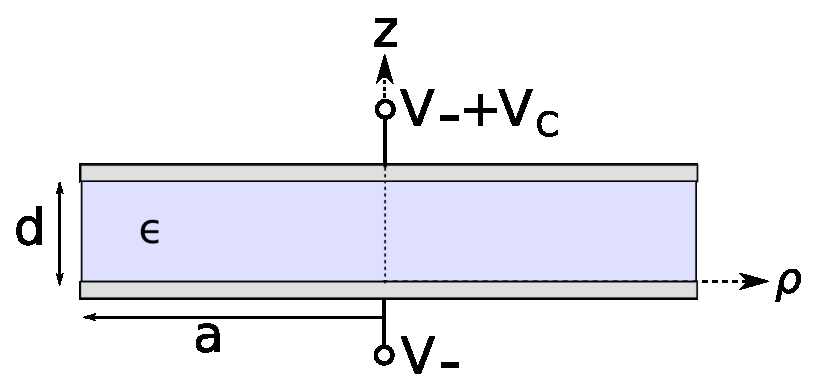
\includegraphics[width=2.5in]{modules/m0068_fPPC.eps}
}}{A parallel plate capacitor, oriented horizontally, with a node above and below the capacitor on the vertical z-axis. The top node is labeled V sub minus plus V sub C. The bottom node is labeled V sub minus. The thin plates on top and bottom are represented by silver lines, and the spacer material between colored blue and labeled epsilon. The distance between the plates is labeled d. From the origin of the z-axis, an arrow extends to the left side of the capacitor, labeled a.  From the origin z-axis pointing to the right, a dashed arrow is labeled rho.}
\end{center} 
\caption{
\label{m0068_fPPC} 
A parallel plate capacitor, as a demonstration of the use of Laplace's Equation.
}
\end{figure}

This problem has cylindrical symmetry, so it makes sense to continue to use cylindrical coordinates with the $z$ axis being perpendicular to the plates.
Equation~\ref{m0068_eLaplace} in cylindrical coordinates is:
%
\begin{equation}
\left[ \frac{1}{\rho} \frac{\partial}{\partial \rho} \left( \rho \frac{\partial}{\partial \rho} \right) 
+ \frac{1}{\rho^2} \frac{\partial^2}{\partial \phi^2}
+ \frac{\partial^2}{\partial z^2} \right] V
= 0 
\end{equation}
%
or perhaps a little more clearly written as follows:
%
\begin{equation}
\frac{1}{\rho} \frac{\partial }{\partial \rho} \left( \rho \frac{\partial V}{\partial \rho} \right) 
+ \frac{1}{\rho^2} \frac{\partial^2 V}{\partial \phi^2}
+ \frac{\partial^2 V}{\partial z^2} 
= 0 
\end{equation}
%
Since the problem has radial symmetry, $\partial V/\partial \phi = 0$.
Since $d \ll a$, we expect the fields to be approximately constant with $\rho$ until we get close to the edge of the plates.
Therefore, we assume $\partial V/\partial \rho$ is negligible and can be taken to be zero. 
Thus, we are left with 
%
\begin{equation}
\frac{\partial^2 V}{\partial z^2} \approx 0 ~~ \mbox{for $\rho \ll a$} 
\label{m0068_eDE}
\end{equation}

The general solution to Equation~\ref{m0068_eDE} is obtained simply by integrating both sides twice, yielding
%
\begin{equation}
V(z) = c_1 z + c_2
\label{m0068_eVAC} 
\end{equation}
%
where $c_1$ and $c_2$ are constants that must be consistent with the boundary conditions. 
Thus, we must develop appropriate boundary conditions.
Let the node voltage at the negative ($z=0$) terminal be $V_{-}$.  
Then the voltage at the positive ($z=+d$) terminal is $V_{-}+V_C$.  
Therefore:
%
\begin{flalign}
V(z=0)  &= V_{-} \\
V(z=+d) &= V_{-}+V_C 
\end{flalign}
%
These are the relevant boundary conditions.  
Substituting $V(z=0) = V_{-}$ into Equation~\ref{m0068_eVAC} yields $c_2 = V_{-}$.
Substituting $V(z=+d) = V_{-}+V_C$ into Equation~\ref{m0068_eVAC} yields $c_1 = V_C/d$.  
Thus, the answer to the problem is
%
\begin{equation}
V(z) \approx \frac{V_C}{d} z + V_{-}  ~~ \mbox{for $\rho \ll a$} 
\label{eEP-PEPP1}
\end{equation}
%
Note that the above result is dimensionally correct and confirms that the potential deep inside a ``thin'' parallel plate capacitor changes linearly with distance between the plates.

Further, you should find that application of the equation ${\bf E} = - \nabla V$ (Section~\ref{m0063_Electric_Field_as_the_Gradient_of_Potential}) to the solution above yields the expected result for the electric field intensity: ${\bf E} \approx -\hat{\bf z}V_C/d$.  
This is precisely the result that we arrived at (without the aid of Laplace's Equation) in Section~\ref{m0002_Electric_Field_Intensity}.   

A reasonable question to ask at this point would be, what about the potential field close to the edge of the plates, or, for that matter, beyond the plates?  
The field in this region is referred to as a \emph{fringing field}. 
\index{fringing (field)}
For the fringing field, $\partial V/ \partial \rho$ is no longer negligible and must be taken into account.  In addition, it is necessary to modify the boundary conditions to account for the outside surfaces of the plates (that is, the sides of the plates that face away from the dielectric) and to account for the effect of the boundary between the spacer material and free space. 
These issues make the problem much more difficult.
When an accurate calculation of a fringing field is necessary, it is common to resort to a numerical solution of Laplace's Equation.
Fortunately, accurate calculation of fringing fields is usually not required in practical engineering applications.

\index{capacitor!parallel plate|)}

      \vfill\break
    \section{Boundary Conditions on the Electric Field Intensity (${\bf E}$)}
{\color{blue}\tiny[m0020]}      % This is text associated with the open textbook "Open Electromagnetics"
% See immediately below for author, date
% This work is licensed under the Creative Commons Attribution-ShareAlike 4.0 International License. (CC BY-SA 4.0) 
% To view a copy of the license, visit http://creativecommons.org/licenses/by-sa/4.0/

%ORB TITLE Boundary Conditions on the Electric Field Intensity (${\bf E}$)
%ORB AUTHOR 0        # S.W. Ellingson, Virginia Tech (ellingson@vt.edu)
%ORB DATE 20180806   # yyyymmdd
%ORB ABSTRACT Boundary Conditions on the Electric Field Intensity 

\label{m0020_Boundary_Conditions_on_E} % <-- Must match name of this file and module directory name.  Don't mess with this!

In homogeneous media, electromagnetic quantities vary smoothly and continuously.
At an interface between dissimilar media, however, it is possible for electromagnetic quantities to be discontinuous.
These discontinuities can be described mathematically as \emph{boundary conditions} and used to to constrain solutions for the associated electromagnetic quantities.
In this section, we derive boundary conditions 
\index{boundary conditions}
on the electric field intensity ${\bf E}$.
\index{electric field intensity!boundary conditions}

To begin, consider a region consisting of only two media that meet at an interface defined by the mathematical surface ${\mathcal S}$, as shown in Figure~\ref{m0020_fPEC}.
%
\begin{figure}[b!]
\begin{center}
\pdftooltip{{  % note double braces
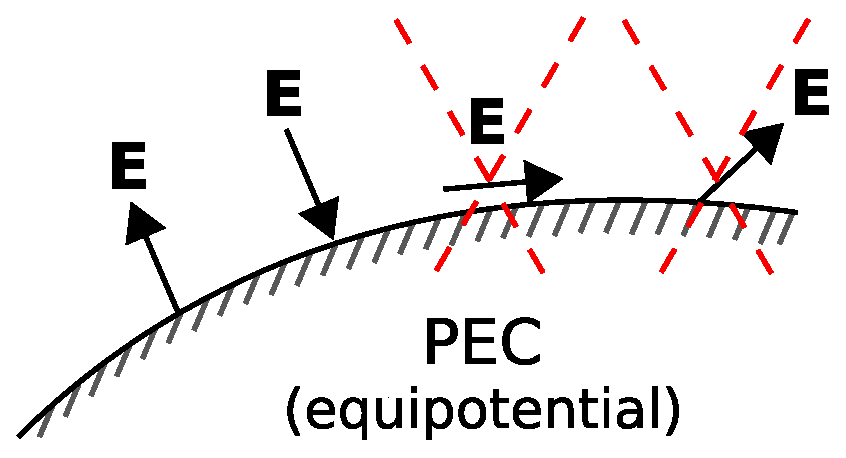
\includegraphics[width=2in]{modules/m0020_fPEC.eps}
% https://commons.wikimedia.org/wiki/File:M0020_fPEC.svg
}}{A curved, arbitrary surface labeled “PEC (equipotential)” shows four vectors labeled E. The leftmost vector is pointed away from the curved surface. The second vector is pointed toward the surface exactly opposite of the leftmost arrow. The third vector is tangent to the surface, pointing to the right, with a dashed red X over it. The fourth vector is at an acute angle to the surface, pointed diagonally to the upper right, with a dashed red X over it. }
\end{center} 
\centerline{\scriptsize 
\copyright~\hyperref[m0020_fPEC_Credit]{K.\ Kikkeri} 
\href{https://creativecommons.org/licenses/by-sa/4.0/}{CC BY~SA 4.0} 
} 
\caption{
\label{m0020_fPEC}
At the surface of a perfectly-conducting region, ${\bf E}$ may be perpendicular to the surface (two leftmost possibilities), but may not exhibit a component that is tangent to the surface (two rightmost possibilities).
}
\end{figure}
%
If either one of the materials is a perfect electrical conductor (PEC), 
\index{conductor!perfect}
then ${\mathcal S}$ is an equipotential surface; i.e., the electric potential $V$ is constant everywhere on ${\mathcal S}$.  
Since ${\bf E}$ is proportional to the spatial rate of change of potential (recall ${\bf E}=-\nabla V$; Section~\ref{m0063_Electric_Field_as_the_Gradient_of_Potential}), we find:
%
%ORB HIGHLIGHT
\begin{mdframed}[backgroundcolor=yellow!20,nobreak=true] 
The component of ${\bf E}$ that is tangent to a perfectly-conducting surface is zero.
\end{mdframed}
%
This is sometimes expressed informally as follows:
%
\begin{equation}
\boxed{
E_{tan} = 0~~\mbox{on PEC surface}
}
\end{equation}
%
where ``$E_{tan}$'' is understood to be the component of ${\bf E}$ that is tangent to ${\mathcal S}$. 
Since the tangential component of ${\bf E}$ on the surface of a perfect conductor is zero, the electric field at the surface must be oriented entirely in the  
direction perpendicular to the surface, as shown in Figure~\ref{m0020_fPEC}.

The following equation expresses precisely the same idea, but includes the calculation of the tangential component as part of the statement:
%
\begin{equation}
{\bf E} \times \hat{\bf n} = 0~~\mbox{(on PEC surface)}
\label{m0020_eEPECBC}
\end{equation} 
%
where $\hat{\bf n}$ is either normal (i.e., unit vector perpendicular to the surface) to each point on ${\mathcal S}$.
This expression works because the cross product of any two vectors is perpendicular to either vector (Section~\ref{m0006_Vector_Arithmetic}), and any vector which is perpendicular to $\hat{\bf n}$ is tangent to ${\mathcal S}$.

We now determine a more general boundary condition that applies even when neither of the media bordering ${\mathcal S}$ is a perfect conductor.
The desired boundary condition can be obtained directly from Kirchoff's Voltage Law (KVL; Section~\ref{m0016_Kirchoffs_Voltage_Law_Electrostatics_Integral_Form}):
\index{Kirchoff's voltage law!electrostatics}
% 
\begin{equation}  
\oint_{\mathcal{C}}{ {\bf E} \cdot d{\bf l} } = 0
\label{m0020_eKVL}
\end{equation}
% 
Let the closed path of integration take the form of a rectangle centered on ${\mathcal S}$, as shown in Figure~\ref{m0020_fKVL}.
%
\begin{figure}
\begin{center}
\pdftooltip{{  % note double braces
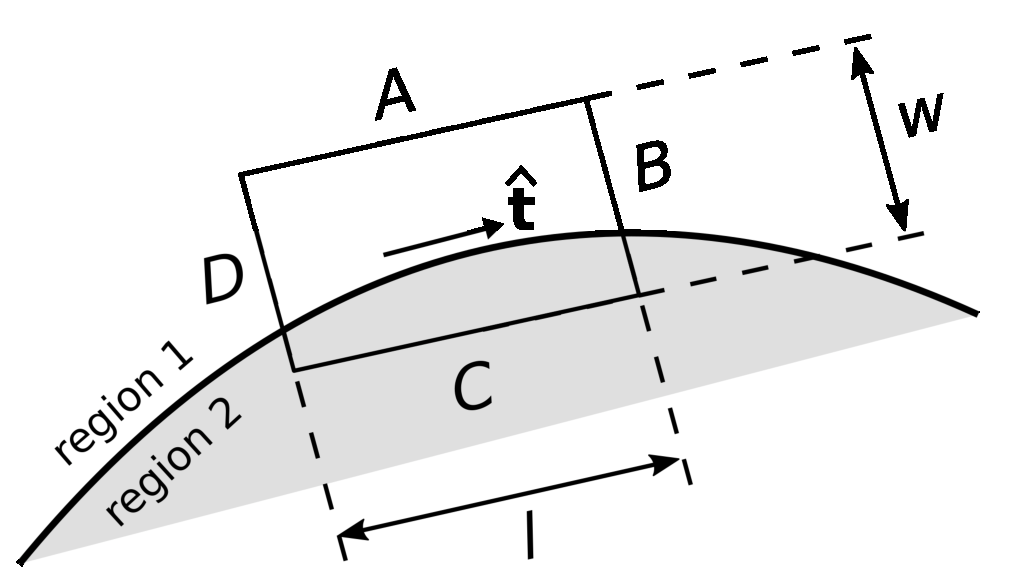
\includegraphics[width=2.5in]{modules/m0020_fKVL.eps}
% https://commons.wikimedia.org/wiki/File:M0020_fKVL.svg
}}{The figure shows a curved arbitrary surface labeled "C", the outside area labeled "region 1" and the inside, greyed area labeled "region 2". A vector tangent to the surface labeled t-hat is pointed to the right. A rectangle is shown surrounding the arrow. Starting with the top side and following a clockwise direction, the rectangle is labeled A, B, C, and D, with A and C being the longer sides. Dashed lines extend on side C with an arrow in between labeled, l. Dashed lines extend on side B with an arrow in between labeled w.}
\end{center} 
\centerline{\scriptsize 
\copyright~\hyperref[m0020_fKVL_Credit]{K.\ Kikkeri} 
\href{https://creativecommons.org/licenses/by-sa/4.0/}{CC BY~SA 4.0} 
} 
\caption{
\label{m0020_fKVL}
Use of KVL to determine the boundary condition on ${\bf E}$.
}
\end{figure}
%
Let the sides $A$, $B$, $C$, and $D$ be perpendicular or parallel to the surface, respectively.  
Let the length of the perpendicular sides be $w$, and let the length of the parallel sides be $l$.  
From KVL we have
% 
\begin{align}   
\oint_{\mathcal{C}}{ {\bf E} \cdot d{\bf l} } &= \int_A{ {\bf E} \cdot d{\bf l} } & \nonumber \\ 
                                &+\int_B{ {\bf E} \cdot d{\bf l} }  & \nonumber \\ 
                                &+\int_C{ {\bf E} \cdot d{\bf l} }  & \nonumber \\
                                &+\int_D{ {\bf E} \cdot d{\bf l} }  &= 0 
\end{align}
%  
Now, let us reduce $w$ and $l$ together while (1) maintaining a constant ratio $w/l\ll 1$ and (2) keeping $\mathcal{C}$ centered on $\mathcal{S}$.
In this process, the contributions from the $B$ and $D$ segments become equal in magnitude but opposite in sign; i.e., 
% 
\begin{equation}   
\int_B{ {\bf E} \cdot d{\bf l} } 
+\int_D{ {\bf E} \cdot d{\bf l} }
\to 0
\end{equation}
%
This leaves
% 
\begin{equation}   
\oint_{\mathcal{C}}{ {\bf E} \cdot d{\bf l} } \to \int_A{ {\bf E} \cdot d{\bf l} }+\int_C{ {\bf E} \cdot d{\bf l} }  \to 0 
\end{equation}
%
Let us define the unit vector $\hat{\bf t}$ (``tangent'') as shown in Figure~\ref{m0020_fKVL}.
When the lengths of sides $A$ and $C$ become sufficiently small, we can write the above expression as follows:
% 
\begin{equation}   
  {\bf E}_1 \cdot \hat{\bf t}\Delta l
- {\bf E}_2 \cdot \hat{\bf t}\Delta l 
\to 0
\label{m0020_eKVL2}
\end{equation}
%
where ${\bf E}_1$ and ${\bf E}_2$ are the fields evaluated on the two sides of the boundary and
$\Delta l\to 0$ is the length of sides $A$ and $C$ while this is happening.
Note that the only way Equation~\ref{m0020_eKVL2} can be true is if the tangential components of ${\bf E}_1$ and ${\bf E}_2$ are equal. In other words: 
%
%ORB HIGHLIGHT
\begin{mdframed}[backgroundcolor=yellow!20,nobreak=true] 
The tangential component of ${\bf E}$ must be continuous across an interface between dissimilar media. 
\end{mdframed}
%
Note that this is a generalization of the result we obtained earlier for the case in which one of the media was a PEC -- in that case, the tangent component of ${\bf E}$ on the other side of the interface must be zero because it is zero in the PEC medium.

As before, we can express this idea in compact mathematical notation.
Using the same idea used to obtain Equation~\ref{m0020_eEPECBC}, we have found
%
\begin{equation}
{\bf E}_1 \times \hat{\bf n} = {\bf E}_2 \times \hat{\bf n}~~~\mbox{on $\mathcal{S}$}
\end{equation}
%
or, as it is more commonly written:
%
\begin{equation}
\boxed{
\hat{\bf n} \times \left( {\bf E}_1 - {\bf E}_2 \right) = 0~~~\mbox{on $\mathcal{S}$}
}
\label{m0020_eBCE}
\end{equation} 

We conclude this section with a note about the broader applicability of this boundary condition:
%
%ORB HIGHLIGHT
\begin{mdframed}[backgroundcolor=yellow!20,nobreak=true] 
Equation~\ref{m0020_eBCE} is the boundary condition that applies to ${\bf E}$ for both the electrostatic \emph{and the general (time-varying) case.}
\end{mdframed}
%
Although a complete explanation is not possible without the use of the Maxwell-Faraday Equation (Section~\ref{m0050_Maxwell-Faraday_Equation}), the reason why this boundary condition applies in the time-varying case can be disclosed here.
In the presence of time-varying magnetic fields, the right-hand side of Equation~\ref{m0020_eKVL} may become non-zero and is proportional to the area defined by the closed loop. 
However, the above derivation requires the area of this loop to approach zero, in which case the possible difference from Equation~\ref{m0020_eKVL} also converges to zero.
Therefore, the boundary condition expressed in Equation~\ref{m0020_eBCE} applies generally.



      \vfill\break
    \section{Boundary Conditions on the Electric Flux Density (${\bf D}$)}
{\color{blue}\tiny[m0021]}      % This is text associated with the open textbook "Open Electromagnetics"
% See immediately below for author, date
% This work is licensed under the Creative Commons Attribution-ShareAlike 4.0 International License. (CC BY-SA 4.0) 
% To view a copy of the license, visit http://creativecommons.org/licenses/by-sa/4.0/

%ORB TITLE Boundary Conditions on the Electric Flux Density (${\bf D}$)
%ORB AUTHOR 0        # S.W. Ellingson, Virginia Tech (ellingson@vt.edu)
%ORB DATE 20180806   # yyyymmdd
%ORB ABSTRACT Boundary Conditions on the Electric Flux Density 

\label{m0021_Boundary_Conditions_on_D} % <-- Must match name of this file and module directory name.  Don't mess with this!
\index{electric flux density!boundary conditions}

In this section, we derive boundary conditions 
\index{boundary conditions}
on the electric flux density ${\bf D}$.
The considerations are quite similar to those encountered in the development of boundary conditions on the electric \emph{field intensity} (${\bf E}$) in Section~\ref{m0020_Boundary_Conditions_on_E}, so the reader may find it useful to review that section before attempting this section.  
This section also assumes familiarity with the concepts of electric flux, electric flux density, and Gauss' Law; for a refresher, Sections~\ref{m0011_Electric_Flux_Density} and \ref{m0014_Gauss_Law_Integral_Form} are suggested. 

To begin, consider a region at which two otherwise-homogeneous media meet at an interface defined by the mathematical surface ${\mathcal S}$, as shown in Figure~\ref{m0021_fPEC}.  Let one of these regions be a perfect electrical conductor (PEC).
\index{conductor!perfect}
%
\begin{figure}[b!]
\begin{center}
\pdftooltip{{  % note double braces
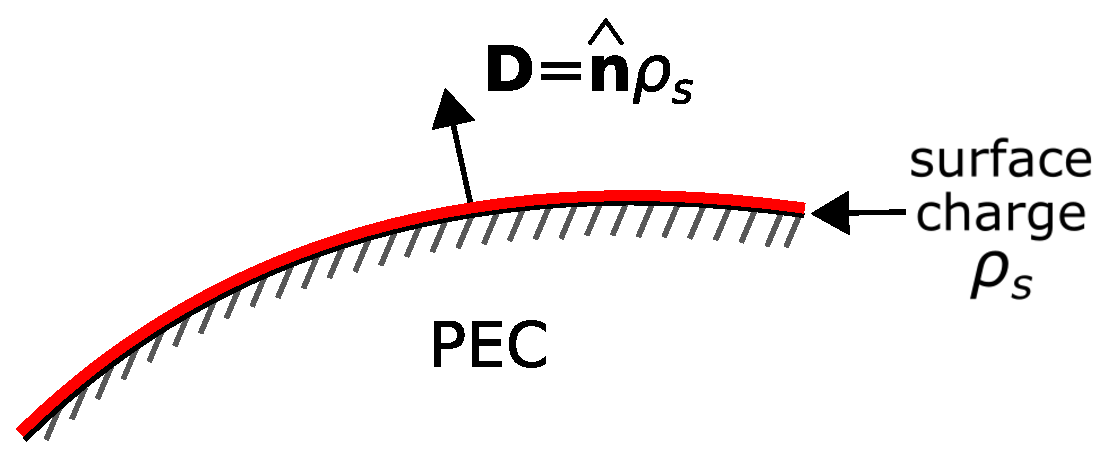
\includegraphics[width=2.5in]{modules/m0021_fPEC.eps}
% https://commons.wikimedia.org/wiki/File:M0021_fPEC.svg
}}{An arbitrary curved surface, labeled PEC. The outside of the surface is colored red, with lines extending at an angle inside the curve of the surface. It is labeled "surface charge rho sub s". An arrow points out of the surface at a perpendicular angle and is labeled bold D = n-hat * rho sub s. }
\end{center} 
\centerline{\scriptsize 
\copyright~\hyperref[m0021_fPEC_Credit]{K.\ Kikkeri} 
\href{https://creativecommons.org/licenses/by-sa/4.0/}{CC BY~SA 4.0} 
} 
\caption{
\label{m0021_fPEC}
The component of ${\bf D}$ that is perpendicular to a perfectly-conducting surface is equal to the charge density on the surface.
}
\end{figure}
%
In Section~\ref{m0020_Boundary_Conditions_on_E}, we established that the tangential component of the electric field must be zero, and therefore, the electric field is directed entirely in the direction perpendicular to the surface.
We further know that the electric field within the conductor is identically zero.
Therefore, ${\bf D}$ at any point on $\mathcal{S}$ is entirely in the direction perpendicular to the surface and pointing into the non-conducting medium.
However, it is also possible to determine the magnitude of ${\bf D}$.
We shall demonstrate in this section that  
%
%ORB HIGHLIGHT
\begin{mdframed}[backgroundcolor=yellow!20,nobreak=true] 
At the surface of a perfect conductor, the magnitude of {\bf D} is equal to the surface charge density $\rho_s$ (units of C/m$^2$) at that point.
\end{mdframed}
%
The following equation expresses precisely the same idea, but includes the calculation of the perpendicular component as part of the statement:
%
\begin{equation}
{\bf D} \cdot \hat{\bf n} = \rho_s~~\mbox{(on PEC surface)}
\label{m0021_eEPECBC}
\end{equation} 
%
where $\hat{\bf n}$ is the normal to ${\mathcal S}$ pointing into the non-conducting region.
(Note that the orientation of $\hat{\bf n}$ is now important;  we have assumed $\hat{\bf n}$ points into region~1, and we must now stick with this choice.)
Before proceeding with the derivation, it may be useful to note that this result is not surprising.  The very definition of electric flux (Section~\ref{m0011_Electric_Flux_Density}) indicates that ${\bf D}$ should correspond in the same way to a surface charge density.  
However, we can show this rigorously, and in the process we can generalize this result to the more-general case in which neither of the two materials are PEC.

The desired more-general boundary condition may be obtained from the integral form of Gauss' Law (Section~\ref{m0014_Gauss_Law_Integral_Form}), as illustrated in Figure~\ref{m0021_fGL}.
%
\begin{figure}
\begin{center}
\pdftooltip{{  % note double braces
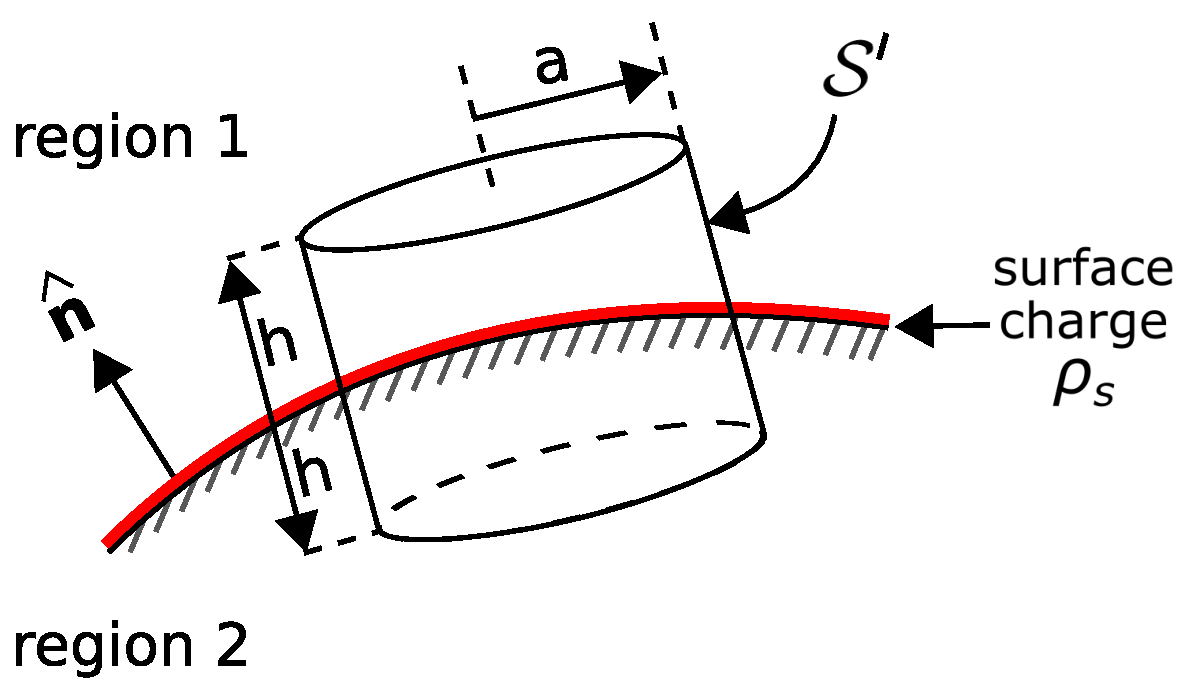
\includegraphics[width=2.5in]{modules/m0021_fGL.eps}
% https://commons.wikimedia.org/wiki/File:M0021_fGL.svg
}}{An arbitrary surface with a surface charge rho sub s. A cylinder drawn with it's midpoint intersecting at a perpendicular angle with the surface. Further details in text.}
\end{center} 
\centerline{\scriptsize 
\copyright~\hyperref[m0021_fGL_Credit]{K.\ Kikkeri} 
\href{https://creativecommons.org/licenses/by-sa/4.0/}{CC BY~SA 4.0} 
} 
\caption{
\label{m0021_fGL}
Use of Gauss' Law to determine the boundary condition on ${\bf D}$.
}
\end{figure}
%
Let the surface of integration $\mathcal{S}'$ take the form of closed cylinder centered at a point on the interface and for which the flat ends are parallel to the surface and perpendicular to $\hat{\bf n}$.  Let the radius of this cylinder be $a$, and let the length of the cylinder be $2h$.  From Gauss' Law we have
%
\begin{align}
\oint_{{\mathcal S}'}{ {\bf D} \cdot d{\bf s} } &= \int_{top} { {\bf D} \cdot d{\bf s} } &            \nonumber \\
                                                 &+ \int_{side} { {\bf D} \cdot d{\bf s} } &            \nonumber \\
                                                 &+ \int_{bottom} { {\bf D} \cdot d{\bf s} } &= Q_{encl} 
\end{align}
%
where 
the ``top'' and ``bottom'' are in Regions~1 and 2, respectively, and
$Q_{encl}$ is the charge enclosed by ${\mathcal S}'$.
Now let us reduce $h$ and $a$ together while (1) maintaining a constant ratio $h/a\ll 1$ and (2) keeping $\mathcal{S}'$ centered on $\mathcal{S}$.
Because $h\ll a$, the area of the side can be made negligible relative to the area of the top and bottom.
Then as $h\to 0$ we are left with  
%
\begin{equation}
\int_{top} { {\bf D} \cdot d{\bf s} } + \int_{bottom} { {\bf D} \cdot d{\bf s} }  \to Q_{encl} 
\end{equation}
%
As the area of the top and bottom sides become infinitesimal, the variation in ${\bf D}$ over these areas becomes negligible.  Now we have simply: 
%
\begin{equation}
{\bf D}_1 \cdot \hat{\bf n}\Delta A + {\bf D}_2 \cdot \left( -\hat{\bf n} \right) \Delta A \to Q_{encl} 
\end{equation}
%
where ${\bf D}_1$ and ${\bf D}_2$ are the electric flux density vectors in medium~1 and medium~2, respectively,
and $\Delta A$ is the area of the top and bottom sides.  
The above expression can be rewritten
%
\begin{equation}
\hat{\bf n} \cdot \left( {\bf D}_1 - {\bf D}_2 \right) \to
\frac{ Q_{encl} }{\Delta A}   
\end{equation}
%
Note that the left side of the equation must represent a actual, physical surface charge; this is apparent from dimensional analysis and the fact that $h$ is now infinitesimally small.  Therefore:
%
\begin{equation}
\boxed{
\hat{\bf n} \cdot \left( {\bf D}_1 - {\bf D}_2 \right) = \rho_s
}
\label{m0021_eBCD}
\end{equation}       
%
where, as noted above, $\hat{\bf n}$ points into region~1.
Summarizing:
%
%ORB HIGHLIGHT
\begin{mdframed}[backgroundcolor=yellow!20,nobreak=true] 
Any discontinuity in the normal component of the electric flux density across the boundary between two material regions is equal to the surface charge.
\end{mdframed}

Now let us verify that this is consistent with our preliminary finding, in which Region~2 was a PEC.
In that case ${\bf D}_2=0$, so we see that Equation~\ref{m0021_eEPECBC} is satisfied, as expected.
If neither Region~1 nor Region~2 is PEC \emph{and} there is no surface charge on the interface, then we find 
$\hat{\bf n} \cdot \left( {\bf D}_1 - {\bf D}_2 \right)=0$; i.e.,
%
%ORB HIGHLIGHT
\begin{mdframed}[backgroundcolor=yellow!20,nobreak=true] 
In the absence of surface charge, the normal component of the electric flux density must be continuous across the boundary.
\end{mdframed}

Finally, we note that since ${\bf D}=\epsilon{\bf E}$, Equation~\ref{m0021_eBCD} implies the following boundary condition on ${\bf E}$:
%
\begin{equation}
\hat{\bf n} \cdot \left( \epsilon_1{\bf E}_1 - \epsilon_2{\bf E}_2 \right) = \rho_s
\label{m0021_eBCE}
\end{equation} 
%
where $\epsilon_1$ and $\epsilon_2$ are the permittivities in Regions~1 and 2, respectively.
The above equation illustrates one reason why we sometimes prefer the ``flux'' interpretation of the electric field to the ``field intensity'' interpretation of the electric field.





      \vfill\break
    \section{Charge and Electric Field for a Perfectly Conducting Region}
{\color{blue}\tiny[m0025]}      % This is text associated with the open textbook "Open Electromagnetics"
% See immediately below for author, date
% This work is licensed under the Creative Commons Attribution-ShareAlike 4.0 International License. (CC BY-SA 4.0) 
% To view a copy of the license, visit http://creativecommons.org/licenses/by-sa/4.0/

%ORB TITLE Charge and Electric Field for a Perfectly Conducting Region
%ORB AUTHOR 0        # S.W. Ellingson, Virginia Tech (ellingson@vt.edu)
%ORB DATE 20180806   # yyyymmdd
%ORB ABSTRACT Charge and Electric Field for a Perfectly Conducting Region

\label{m0025_Charge_and_Electric_Field_for_a_Perfectly_Conducting_Region} % <-- Must match name of this file and module directory name.  Don't mess with this!

In this section, we consider the behavior of charge and the electric field in the vicinity of a perfect electrical conductor (PEC).
\index{conductor!perfect}

First, note that the electric field -- both the electric field intensity {\bf E} and electric flux density {\bf D} -- throughout a PEC region is zero.
This is because the electrical potential throughout a PEC region must be constant.
(This idea is explored further in Section~\ref{m0010_Conductivity}.)
Recall that the electric field is proportional to the spatial rate of change of electrical potential (i.e., ${\bf E}=-\nabla V$; Section~\ref{m0063_Electric_Field_as_the_Gradient_of_Potential}).
Thus, the electric field must be zero throughout a PEC region.

Second, 
the electric field is oriented directly away from (i.e., perpendicular to) the PEC surface, and the magnitude of ${\bf D}$ is equal to the surface charge density $\rho_s$ (C/m$^2$) (Section~\ref{m0021_Boundary_Conditions_on_D}). 

Now we address the question of charge distribution; i.e., the location and density of charge.
Consider the scenario shown in Figure~\ref{m0025_fFlatSlab}.
%
\begin{figure}[b!]
\begin{center}
\pdftooltip{{  % note double braces
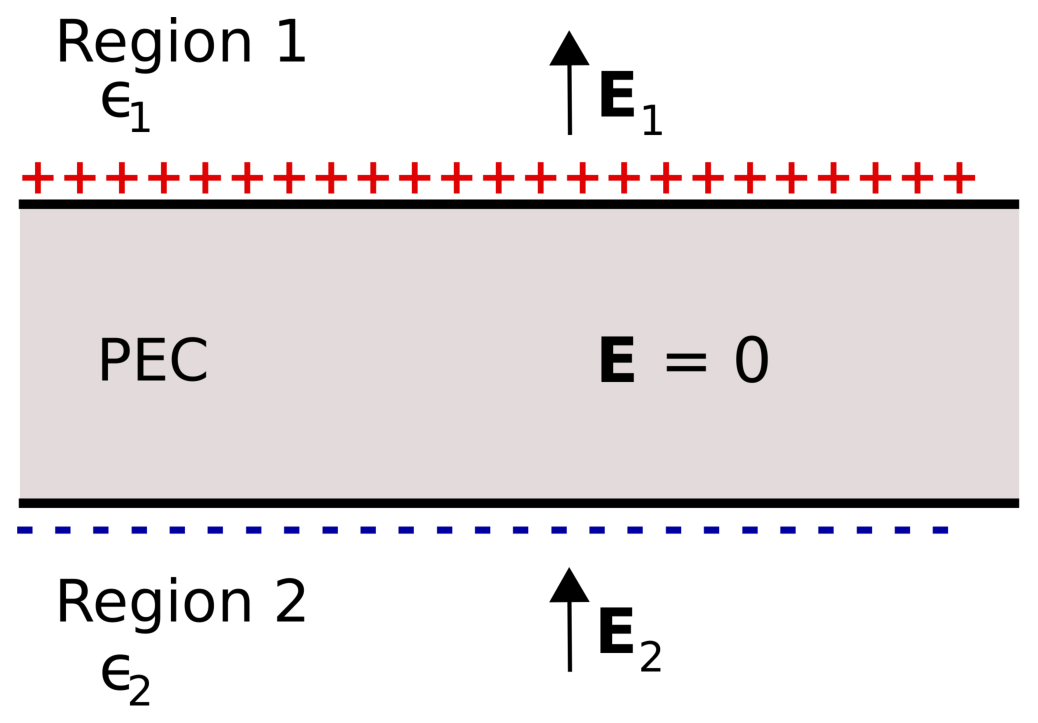
\includegraphics[width=2.5in]{modules/m0025_fFlatSlab.eps}
% https://commons.wikimedia.org/wiki/File:M0025_fFlatSlab.svg
}}{Region 1, above the slab, is shown as positively charged in field E sub 1, and Region 2, below the slab, is shown as negatively charged in E sub 2.}
\end{center} 
\centerline{\scriptsize 
\copyright~\hyperref[m0025_fFlatSlab_Credit]{K.\ Kikkeri}
\href{https://creativecommons.org/licenses/by-sa/4.0/}{CC BY~SA 4.0} 
} 
\caption{
\label{m0025_fFlatSlab}
An infinite flat slab of PEC in the presence of an applied electric field. 
}
\end{figure}
%
Here, a flat slab of PEC material is embedded in dielectric material.\footnote{For the purposes of this section, it suffices to interpret ``dielectric'' as a ``nonconducting and well characterized entirely in terms of its permittivity.''  For more, see Section~\ref{m0107_Dielectric_Media}.}
The thickness of the slab is finite, whereas the length and width of the slab is infinite.
The region above the slab is defined as Region~1 and has permittivity $\epsilon_1$.
The region below the slab is defined as Region~2 and has permittivity $\epsilon_2$.
Electric fields ${\bf E}_1$ and ${\bf E}_2$ are present in Regions~1 and 2, respectively, as shown in Figure~\ref{m0025_fFlatSlab}.
To begin, let us assume that these fields are the result of some external stimulus that results in the direction of these fields being generally upward, as shown in Figure~\ref{m0025_fFlatSlab}.

Now, what do we know about ${\bf E}_1$ and ${\bf E}_2$?
First, both fields must satisfy the relevant boundary conditions.
That is, the component of ${\bf E}_1$ that is tangent to the upper PEC surface is zero, so that ${\bf E}_1$ is directed entirely in a direction perpendicular to the surface.  
Similarly, the component of ${\bf E}_2$ that is tangent to the lower PEC surface is zero, so that ${\bf E}_2$ is directed entirely in a direction perpendicular to the surface. 
At this point we have not determined the magnitudes or signs of ${\bf E}_1$ and ${\bf E}_2$; we have established only that there are no non-zero components tangential to (i.e., parallel to) the PEC surfaces.

Next, recall that the electric field must be zero within the slab. 
This means that there must be zero net charge within the slab, since any other distribution of charge will result in a non-zero electric field, and subsequently a potential difference between locations within the slab. 
Therefore:
%
%ORB HIGHLIGHT
\begin{mdframed}[backgroundcolor=yellow!20,nobreak=true] 
There can be no static charge \emph{within} a PEC. 
\end{mdframed}
%
It follows that
%
%ORB HIGHLIGHT
\begin{mdframed}[backgroundcolor=yellow!20,nobreak=true] 
Charge associated with a PEC lies entirely on the surface. 
\end{mdframed}

Outside the slab, the boundary conditions on ${\bf D}_1$ and ${\bf D}_2$ in the dielectric regions require these fields to be non-zero when the surface charge density on the PEC is non-zero.
The surface charge supports the discontinuity in the normal component of the electric fields.
Specifically, ${\bf D}_1$ and ${\bf D}_2$ have the same magnitude $\left|\rho_s\right|$ because the surface charge densities on both sides of the slab have equal magnitude.
However, the electric field intensity ${\bf E}_1={\bf D}_1/\epsilon_1$, whereas ${\bf E}_2={\bf D}_2/\epsilon_2$; i.e., these are different.
That is, the electric field intensities are unequal unless the permittivities in each dielectric region are equal.

%%% ORIGINAL VERSION OF PARAGRAPH, USES SINGLE CUBE AS AN EXAMPLE %%%%%%%%%%%%%%%%%%%%%%%%% 
%% TODO: Maybe make this a problem?
% Finally, let us consider the effect if the length and width of the slab are reduced from infinity, forming a cube in which the length of each side is equal to the thickness of the original slab.  This is shown in Figure~\ref{m0025_fCube}.  For simplicity we have also set $\epsilon_1=\epsilon_2$, so the conductor is embedded in a single homogeneous material.  In this case the situation is as shown in Figure~\ref{m0025_fCube}.  Note that electric field lines now bend in the dielectric so as to satisfy the requirement that the tangential component of the electric field be zero on the surface of the cube.  Also note that the charge distribution arranges itself on the surface of the cube so as to maintain constant potential within the cube.
%
% \begin{figure}
% \begin{center}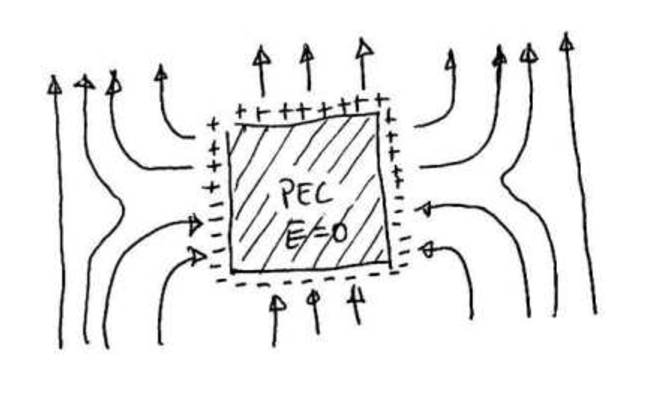
\includegraphics[width=2.5in]{modules/m0025_fCube.eps}\end{center} 
% %\vspace{2in}
% % ***WikipediaCommonsURL
% %\centerline{\scriptsize 
% %\copyright~\hyperref[***_Credit]{author} 
% %\href{https://creativecommons.org/licenses/by-sa/4.0/}{CC BY~SA 4.0} 
% %} 
% \caption{
% \label{m0025_fCube}
% A PEC cube in the presence of an applied electric field. 
% }
% \end{figure}

%%% NEW VERSION OF PARAGRAPH, USES FOUND FIGURE (POINT CHARGE AND MULTIPLE SHAPES) INSTEAD OF SINGLE CUBE %%%%%%%%%%%%%%%%%%%%%%%%% 
Finally, let us consider the structure of the electric field in more general cases.  
Figure~\ref{m0025_fPEC_field_lines} shows field lines in a homogeneous dielectric material in which a point charge and PEC regions of various shapes are embedded. 
Note that electric field lines now bend in the dielectric so as to satisfy the requirement that the tangential component of the electric field be zero on PEC surfaces.
Also note that the charge distribution arranges itself on the PEC surfaces so as to maintain zero electric field and constant potential within the cube.
%
\begin{figure}
\begin{center}
\pdftooltip{{  % note double braces
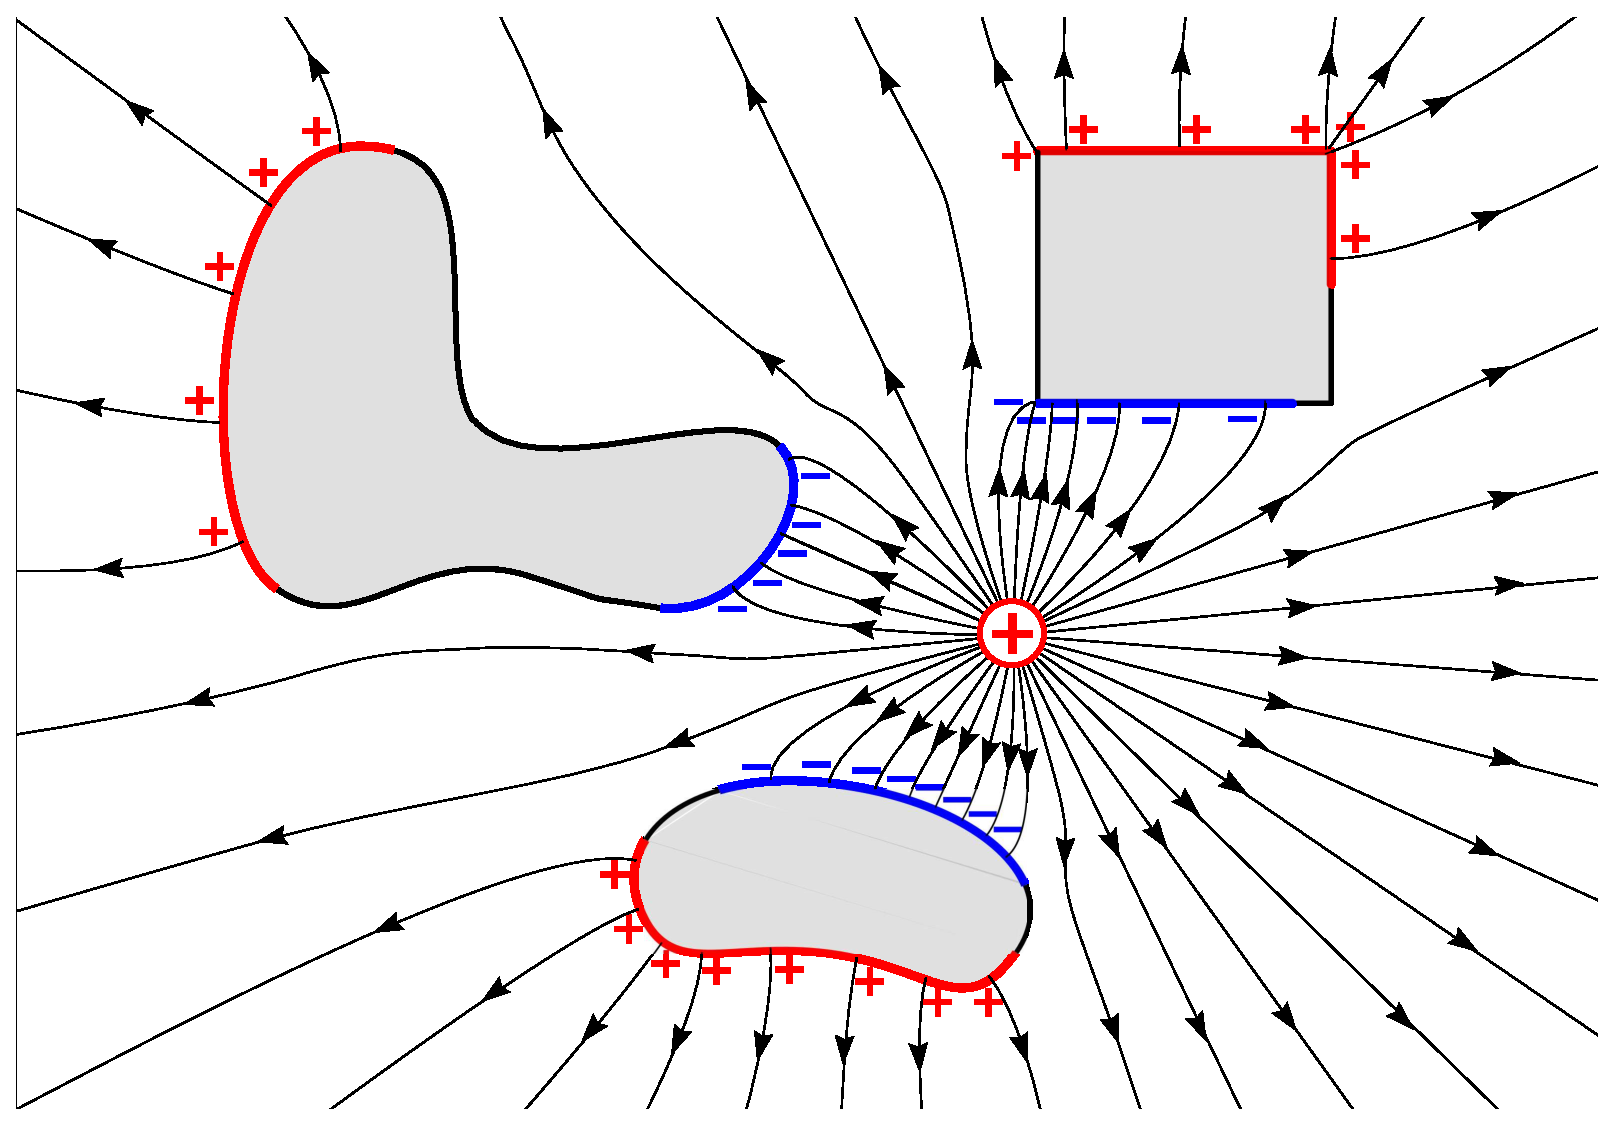
\includegraphics[width=\columnwidth]{modules/m0025_Electrostatic_induction_SE170813.eps}
% https://commons.wikimedia.org/wiki/File:Electrostatic_induction.svg
}}{A positive point charge is surrounded by three arbitrary, grey shaped PEC regions: one to the upper right, one to the directly below, and one to the upper left. From that particle extends electric field lines in all directions. Where the electric field lines meet the arbitrary regions the regions are labeled negative.}
\end{center} 
\centerline{\scriptsize 
by~\hyperref[m0025_fPEC_field_lines_Credit]{C.\ Burks} (modified) 
% public domain
} 
\caption{
\label{m0025_fPEC_field_lines}
Electric field lines due to a point charge in the vicinity of PEC regions (shaded) of various shapes. 
}
\end{figure}


      \vfill\break
    \section{Dielectric Media}
{\color{blue}\tiny[m0107]}      % This is text associated with the open textbook "Open Electromagnetics"
% See immediately below for author, date
% This work is licensed under the Creative Commons Attribution-ShareAlike 4.0 International License. (CC BY-SA 4.0) 
% To view a copy of the license, visit http://creativecommons.org/licenses/by-sa/4.0/

%ORB TITLE Dielectric Media
%ORB AUTHOR 0        # S.W. Ellingson, Virginia Tech (ellingson@vt.edu)
%ORB DATE 20180806   # yyyymmdd
%ORB ABSTRACT Dielectric Media

\label{m0107_Dielectric_Media} % <-- Must match name of this file and module directory name.  Don't mess with this!
\index{dielectric (material)|(}

\emph{Dielectric} is particular category of materials that exhibit low conductivity\footnote{See Section~\ref{m0007_Properties_of_Materials} for a refresher on parameters describing properties of materials.} because their constituent molecules remain intact when exposed to an electric field, as opposed to shedding electrons as is the case in good conductors.
Subsequently, dielectrics do not effectively pass current, and are therefore considered ``good insulators'' 
\index{insulator!good}
as well as ``poor conductors.'' 
\index{conductor!poor}
An important application of dielectrics in electrical engineering is as a spacer material in printed circuit boards (PCBs), coaxial cables, and capacitors.

Examples of dielectrics include air, 
\index{air}
glass, \index{glass}
teflon, \index{teflon}
 and fiberglass epoxy (the material used in common ``FR4'' 
\index{FR4}
printed circuit boards). 
\index{printed circuit board (PCB)}
These and other dielectrics are listed along with values of their constitutive parameters in Section~\ref{m0135_Table_of_Permittivities}.

The electromagnetic properties of dielectric materials are quantified primarily by relative permittivity 
\index{permittivity!relative}
$\epsilon_r$ (Section~\ref{m0008_Permittivity}), which ranges from very close to 1 upward to roughly 50, and is less than 6 or so for most commonly-encountered materials having low moisture content.  
The permeability 
\index{permeability}
of dielectric materials is approximately equal to the free-space value (i.e., $\mu\approx\mu_0$); therefore, these materials are said to be ``non-magnetic.''
\index{non-magnetic (material)} 

{\bf Additional Reading:}
\begin{itemize}
\item ``\href{https://en.wikipedia.org/wiki/Dielectric}{Dielectric}'' on Wikipedia.
\end{itemize}

\index{dielectric (material)|)}

      \vfill\break
    \section{Dielectric Breakdown}
{\color{blue}\tiny[m0109]}      % This is text associated with the open textbook "Open Electromagnetics"
% See immediately below for author, date
% This work is licensed under the Creative Commons Attribution-ShareAlike 4.0 International License. (CC BY-SA 4.0) 
% To view a copy of the license, visit http://creativecommons.org/licenses/by-sa/4.0/

%ORB TITLE Dielectric Breakdown
%ORB AUTHOR 0        # S.W. Ellingson, Virginia Tech (ellingson@vt.edu)
%ORB DATE 20180806   # yyyymmdd
%ORB ABSTRACT Dielectric Breakdown

\label{m0109_Dielectric_Breakdown} % <-- Must match name of this file and module directory name.  Don't mess with this!

The permittivity 
\index{permittivity}
of an ideal dielectric is independent of the magnitude of an applied electric field; the material is said to be ``linear.''\footnote{See Section~\ref{m0007_Properties_of_Materials} for a review of this concept.}
\index{linear (media)}
However, all practical dielectrics fail in this respect with sufficiently strong electric field.
Typically, the failure is abrupt and is observed as a sudden, dramatic increase in conductivity, signaling that electrons are being successfully dislodged from their host molecules.
The threshold value of the electric field intensity at which this occurs is known as the \emph{dielectric strength}, 
\index{dielectric strength}
and the sudden change in behavior observed in the presence of an electric field greater than this threshold value is known as \emph{dielectric breakdown}.
\index{dielectric breakdown}

Dielectric strength varies from about 3~MV/m for air to about 200~MV/m in mica 
\index{mica}
(a dielectric commonly used in capacitors).

Dielectric breakdown is typically accompanied by ``arcing,'' 
\index{arcing}
which is a sudden flow of current associated with the breakdown.
A well known example of this phenomenon is lightning, 
\index{lightning}
which occurs when charge is exchanged between sky and ground when air
\index{air}
(a dielectric) exhibits breakdown.
Dielectric breakdown in solids typically damages the material. 

{\bf Additional Reading:}
\begin{itemize}
\item ``\href{https://en.wikipedia.org/wiki/Electrical_breakdown}{Electrical Breakdown}'' on Wikipedia.
\end{itemize}



      \vfill\break
    \section{Capacitance}
{\color{blue}\tiny[m0112]}      % This is text associated with the open textbook "Open Electromagnetics"
% See immediately below for author, date
% This work is licensed under the Creative Commons Attribution-ShareAlike 4.0 International License. (CC BY-SA 4.0) 
% To view a copy of the license, visit http://creativecommons.org/licenses/by-sa/4.0/

%ORB TITLE Capacitance
%ORB AUTHOR 0        # S.W. Ellingson, Virginia Tech (ellingson@vt.edu)
%ORB DATE 20180806   # yyyymmdd
%ORB ABSTRACT Capacitance

\label{m0112_Capacitance} % <-- Must match name of this file and module directory name.  Don't mess with this!
\index{capacitance|(}

When separate regions of positive and negative charge exist in proximity, Coulomb forces (Section~\ref{m0102_Coulombs_Law}) will attempt to decrease the separation between the charges.
As noted in Section~\ref{m0061_Force_Energy_and_Potential_Difference}, this can be interpreted as a tendency of a system to reduce its potential energy.
If the charges are fixed in place, then the potential energy remains constant.  
This potential energy is proportional to the Coulomb force.
Referring back to Section~\ref{m0102_Coulombs_Law}, the Coulomb force is:
%
\begin{itemize}
\item Proportional to quantity of positive charge squared  
\item Inversely proportional to the separation between the charges squared
\item Inversely proportional to the permittivity of the material separating the charges
\end{itemize}
Therefore, the potential energy of the system is likewise dependent on charge, separation, and permittivity.
Furthermore, we see that the ability of a system to store energy in this manner depends on the geometry of the charge distribution and the permittivity of the intervening material.  

Now recall that the electric field intensity ${\bf E}$ 
\index{electric field intensity}
is essentially defined in terms of the Coulomb force; 
\index{force}
i.e., ${\bf F}=q{\bf E}$ (Section~\ref{m0002_Electric_Field_Intensity}).
So, rather than thinking of the potential energy of the system as being associated with the Coulomb force, it is equally valid to think of the potential energy as being stored in the electric field associated with the charge distribution.
It follows from the previous paragraph that the energy stored in the electric field depends on the geometry of the charge distribution and the permittivity of the intervening media.  
This relationship is what we mean by \emph{capacitance}.
We summarize as follows:
%
%ORB HIGHLIGHT
\begin{mdframed}[backgroundcolor=yellow!20,nobreak=true] 
Capacitance 
\index{capacitance!definition}
is the ability of a structure to store energy in an electric field.
\end{mdframed}
%
and
%
%ORB HIGHLIGHT
\begin{mdframed}[backgroundcolor=yellow!20,nobreak=true] 
The capacitance of a structure depends on its geometry and the permittivity of the medium separating regions of positive and negative charge.
\end{mdframed}

Note that capacitance does \emph{not} depend on charge, which we view as either a stimulus or response from this point of view.
The corresponding response or stimulus, respectively, is the potential associated with this charge.
This leads to the following definition:
%
\begin{equation}
\boxed{
C \triangleq \frac{Q_+}{V}
}
\label{m0112_Cdef}
\end{equation} 
%
where $Q_+$ (units of C) is the total positive charge, $V$ (units of V) is the potential associated with this charge (defined such that it is positive),  and $C$ (units of F) is the associated capacitance. So:
%
%ORB HIGHLIGHT
\begin{mdframed}[backgroundcolor=yellow!20,nobreak=true] 
In practice, capacitance is defined as the ratio of charge present on one conductor of a two-conductor system to the potential difference between the conductors (Equation~\ref{m0112_Cdef}). 
\end{mdframed}
%
In other words, a structure is said to have greater capacitance if it stores more charge -- and therefore stores more energy -- in response to a given potential difference.

Figure~\ref{m0112_fGenericCap} shows the relevant features of this definition.
Here, a battery imposes the potential difference $V$ between two regions of perfectly-conducting material.
$Q_+$ is the total charge on the surface of the PEC region attached to the positive terminal of the battery.
An equal amount of negative charge appears on the surface of the PEC region attached to the negative terminal of the battery (Section~\ref{m0025_Charge_and_Electric_Field_for_a_Perfectly_Conducting_Region}).
This charge distribution gives rise to an electric field.
Assuming the two PEC regions are fixed in place, $Q_+$ will increase linearly with increasing $V$, at a rate determined by the capacitance $C$ of the structure. 
%
\begin{figure}
\begin{center}
\pdftooltip{{  % note double braces
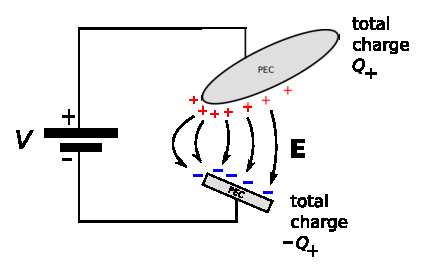
\includegraphics[width=2.5in]{modules/m0112_fGenericCap.eps}
}}{The figure shows a battery with each side connected to a distinct arbitrary, grey region labeled PEC. The regions are parallel. The upper shape is attached to the positive end of the battery has a total charge Q super +. The lower shape is attached to the negative end, with a total charge -Q super +. In the space between the two shapes is an electric field pointing from the upper shape (positive) to the lower shape (negative), labeled E.}
\end{center} 
%\centerline{\scriptsize 
%\copyright~\hyperref[m0112_fGenericCap_Credit]{author} 
%\href{https://creativecommons.org/licenses/by-sa/4.0/}{CC BY~SA 4.0} 
%} 
\caption{
\label{m0112_fGenericCap}
Electrostatic interpretation of capacitance.
}
\end{figure}

\index{capacitor|(}

A \emph{capacitor} is a device that is designed to exhibit a specified capacitance.
We can now make the connection to the concept of the capacitor as it appears in elementary circuit theory.
In circuit theory, the behavior of devices is characterized in terms of terminal voltage $V_T$ in response to terminal current $I_T$, and vice versa.
First, note that current does not normally flow through a capacitor,\footnote{If it does, it's probably experiencing \emph{dielectric breakdown}; see Section~\ref{m0109_Dielectric_Breakdown}.} so when we refer to ``terminal current'' for a capacitor, what we \emph{really} mean is the flow of charge arriving or departing from one of the conductors via the circuit, which is equal to the flow of charge departing or arriving (respectively) at the other conductor.  This gives the appearance of current flow through the capacitor when the current is examined from outside the capacitor.
With that settled, we proceed as follows.
Using Equation~\ref{m0112_Cdef}, we express the voltage $V_T$ across the terminals of a capacitor having capacitance $C$:
%
\begin{equation}
V_T = \frac{Q_+}{C}
\end{equation}
%
We seek a relationship between $V_T$ and $I_T$.
Current is charge per unit time, so the charge on either conductor is the integral of $I_T$ over time; i.e.:
%
\begin{equation}
Q_+(t) = \int_{t_0}^{t} { I_T(\tau)~d\tau } + Q_+(t_0)
\end{equation}
%
where $t_0$ is an arbitrarily-selected start time.
In other words, amps integrated over time is charge. If we define $I_T$ as being positive in the direction of the flow of positive charge as is the usual convention, then we have:
%
\begin{equation}
V_T(t) = \frac{1}{C}\int_{t_0}^{t} { I_T(\tau)~d\tau } + \frac{1}{C}Q_+(t_0)
\end{equation}
%
Again applying Equation~\ref{m0112_Cdef}, we see that the second term is simply $V_T(t_0)$.
This is the expected relationship from elementary circuit theory.

Finally, solving for $I_T$ we obtain the differential form of this relationship:
%
\begin{equation}
I_T(t) = C\frac{d}{dt}V_T(t)
\end{equation}

\index{capacitor|)}

%%%%%%%%%%%%%%%%%%%%%%%%%%%%%%%%%%%%%%%%%%%%

{\bf Additional Reading:}
\begin{itemize}
\item ``\href{https://en.wikipedia.org/wiki/Capacitance}{Capacitance}'' on Wikipedia.
\item ``\href{https://en.wikipedia.org/wiki/Capacitor}{Capacitor}'' on Wikipedia.
\end{itemize}

\index{capacitance|)}

      \vfill\break
    \section{The Thin Parallel Plate Capacitor}
{\color{blue}\tiny[m0070]}      % This is text associated with the open textbook "Open Electromagnetics"
% See immediately below for author, date
% This work is licensed under the Creative Commons Attribution-ShareAlike 4.0 International License. (CC BY-SA 4.0) 
% To view a copy of the license, visit http://creativecommons.org/licenses/by-sa/4.0/

%ORB TITLE The Thin Parallel Plate Capacitor
%ORB AUTHOR 0        # S.W. Ellingson, Virginia Tech (ellingson@vt.edu)
%ORB DATE 20180806   # yyyymmdd
%ORB ABSTRACT Thin parallel plate capacitor

\label{m0070_Parallel_Plate_Capacitor_Capacitance_from_Charge} % <-- Must match name of this file and module directory name.  Don't mess with this!
\index{capacitor!parallel plate|(}

Let us now determine the capacitance of a common type of capacitor known as the \emph{thin parallel plate capacitor}, 
shown in Figure~\ref{m0070_fPPCap}.
This capacitor consists of two flat plates, each having area $A$, separated by distance $d$.
To facilitate discussion, let us place the origin of the coordinate system at the center of the lower plate, with the $+z$ axis directed toward the upper plate such that the upper plate lies in the $z=+d$ plane.
%
\begin{figure}[b!]
\begin{center}
\pdftooltip{{  % note double braces
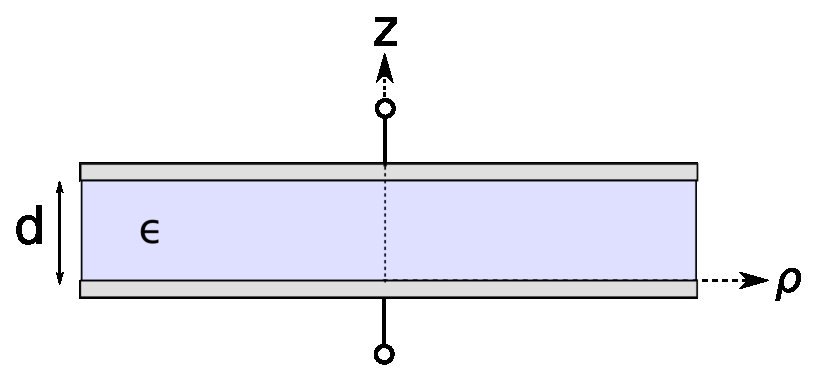
\includegraphics[width=2.5in]{modules/m0070_fPPCap.eps}
%% https://en.wikipedia.org/wiki/File:Parallel_plate_capacitor.svg
}}{A parallel plate capacitor lying horizontal with a node above and below the capacitor drawn on the x-axis similar to a previous figure. The thin plates on top and bottom are represented by silver lines, and the spacer material between colored blue and labeled epsilon. The distance between the plates is labeled d. A dashed arrow points from the z-axis out of the bottom right side of the capacitor, labeled rho.}
\end{center} 
%\centerline{\scriptsize 
%by~\hyperref[m0070_fPPCap_Credit]{inductiveload} (modified)
%%\href{https://creativecommons.org/licenses/by-sa/4.0/}{CC BY-SA 4.0} 
%} 
\caption{
\label{m0070_fPPCap}
Thin parallel plate capacitor.
}
\end{figure}

Below we shall find the capacitance by assuming a particular charge on one plate, using the boundary condition on the electric flux density ${\bf D}$ to relate this charge density to the internal electric field, and then integrating over the electric field between the plates to obtain the potential difference.  Then, capacitance is the ratio of the assumed charge to the resulting potential difference.

The principal difficulty in this approach is finding the electric field. 
To appreciate the problem, first consider that if the area of the plates was infinite, then the electric field would be very simple; it would begin at the positively-charged plate and extend in a perpendicular direction toward the negatively-charged plate (Section~\ref{m0025_Charge_and_Electric_Field_for_a_Perfectly_Conducting_Region}).  Furthermore, the field would be constant everywhere between the plates.  This much is apparent from symmetry alone.
However, when the plate area is finite, then we expect a \emph{fringing field} 
\index{fringing (field)}
to emerge.  ``Fringing field'' is simply a term applied to the non-uniform field that appears near the edge of the plates. The field is non-uniform in this region because the boundary conditions on the \emph{outside} (outward-facing) surfaces of the plates have a significant effect in this region. 
In the central region of the capacitor, however, the field is not much different from the field that exists in the case of infinite plate area.

In any parallel plate capacitor having finite plate area, some fraction of the energy will be stored by the approximately uniform field of the central region, and the rest will be stored in the fringing field.  We can make the latter negligible relative to the former by making the capacitor very ``thin,'' in the sense that the smallest identifiable dimension of the plate is much greater than $d$.  
Under this condition, we may obtain a good approximation of the capacitance by simply neglecting the fringing field, since an insignificant fraction of the energy is stored there.

Imposing the ``thin'' condition leads to three additional simplifications.  
First, the surface charge distribution may be assumed to be approximately uniform over the plate, which greatly simplifies the analysis.
Second, the shape of the plates becomes irrelevant; they might be circular, square, triangular, etc. 
When computing capacitance in the ``thin'' case, only the plate area $A$ is important. 
Third, the thickness of each of the plates becomes irrelevant.

We are now ready to determine the capacitance of the thin parallel plate capacitor.  Here are the steps:
%  
\begin{enumerate}
\item Assume a total positive charge $Q_+$ on the upper plate.
\item Invoking the ``thin'' condition, we assume the charge density on the plates is uniform.  Thus, the surface charge density on bottom side of the upper plate is $\rho_{s,+} = Q_+/A$ (C/m$^2$).  
\item \label{m0070_iStep1} From the boundary condition on the bottom surface of the upper plate, ${\bf D}$ on this surface is $-\hat{\bf z}\rho_{s,+}$. 
\item The total charge on the lower plate, $Q_-$, must be equal and opposite the total charge on the upper plate; i.e, $Q_-=-Q_+$.  Similarly, the surface charge density on the upper surface of the lower plate, $\rho_{s,-}$, must be $-\rho_{s,+}$.
\item 
From the boundary condition on the top surface of the lower plate (Section~\ref{m0021_Boundary_Conditions_on_D}), ${\bf D}$ on this surface is $+\hat{\bf z}\rho_{s,-}$.  
Since $+\hat{\bf z}\rho_{s,-}=-\hat{\bf z}\rho_{s,+}$, ${\bf D}$ on the facing sides of the plates is equal. 
\item Again invoking the ``thin'' condition, we assume ${\bf D}$ between the plates has approximately the same structure as we would see if the plate area was infinite.  Therefore, we are justified in assuming ${\bf D}\approx-\hat{\bf z}\rho_{s,+}$ \emph{everywhere} between the plates.  (You might also see that this is self-evident from the definition of ${\bf D}$ as the flux density of electric charge (Section~\ref{m0011_Electric_Flux_Density}).)
\item With an expression for the electric field in hand, we may now compute the potential difference $V$ between the plates as follows (Section~\ref{m0061_Force_Energy_and_Potential_Difference}):
%
\begin{flalign}
V &= -\int_{\mathcal C}{ {\bf E} \cdot d{\bf l} }  \nonumber \\
  &= -\int_{0}^{d}{ \left(\frac{1}{\epsilon}{\bf D}\right) \cdot \left(\hat{\bf z}dz\right) } \nonumber \\
  &= -\int_{0}^{d}{ \left(-\hat{\bf z}\frac{\rho_{s,+}}{\epsilon}\right) \cdot \left(\hat{\bf z}dz\right) } \nonumber \\
  &= +\frac{\rho_{s,+}~d}{\epsilon}
\end{flalign} 
%
\item Finally,
%
\begin{equation}
C = \frac{Q_+}{V} = \frac{\rho_{s,+}~A}{\rho_{s,+}~d/\epsilon} = \frac{\epsilon A}{d}
\end{equation}
%
\end{enumerate}

Summarizing:
%
\begin{equation}
\boxed{
C \approx \frac{\epsilon A}{d}
}
\label{m0070_eTPPC}
\end{equation}
%
%ORB HIGHLIGHT
\begin{mdframed}[backgroundcolor=yellow!20,nobreak=true] 
The capacitance of a parallel plate capacitor having plate separation much less than the size of the plate is given by Equation~\ref{m0070_eTPPC}.
This is an approximation because the fringing field is neglected. 
\end{mdframed}
%
It's worth noting that this is dimensionally correct; i.e., F/m times m$^2$ divided by m yields F.
It's also worth noting the effect of the various parameters:
%
%ORB HIGHLIGHT
\begin{mdframed}[backgroundcolor=yellow!20,nobreak=true] 
Capacitance increases in proportion to permittivity and plate area and decreases in proportion to distance between the plates.
\end{mdframed}

\index{printed circuit board (PCB)!capacitance|(}
%ORB EXAMPLE
~\\ \begin{example} 
\begin{mdframed}[backgroundcolor=brown!20,linecolor=brown!20]\raggedright
Printed circuit board capacitance. 
\\~\\
Printed circuit boards commonly include a ``ground plane,'' 
\index{ground plane}
which serves as the voltage datum for the board, and at least one ``power plane,'' which is used to distribute a DC supply voltage (See ``Additional Reading'' at the end of this section).  These planes are separated by a dielectric material, and the resulting structure exhibits capacitance.  This capacitance may be viewed as an equivalent discrete capacitor in parallel with the power supply. 
The value of this equivalent capacitor may be either negligible, significant and beneficial, or significant and harmful.  So, it is useful to know the value of this equivalent capacitor.   

For a common type of circuit board, the dielectric thickness is about 1.6~mm and the relative permittivity of the material is about 4.5.  If the area in common between the ground and power planes is 25~cm$^2$, what is the value of the equivalent capacitor?

{\bf Solution.}
From the problem statement, 
$\epsilon\cong 4.5\epsilon_0$, 
$A \cong 25$~cm$^2$ $=$ $2.5~\times 10^{-3}$~m$^2$, and
$d \cong 1.6$~mm.
Using Equation~\ref{m0070_eTPPC}, the value of the equivalent capacitor is $62.3$~pF.

\end{mdframed}\end{example}

\index{printed circuit board (PCB)!capacitance|)}

%%%%%%%%%%%%%%%%%%%%%%%%%%%%%%%%%%%%

{\bf Additional Reading:}
\begin{itemize}
\item ``\href{https://en.wikipedia.org/wiki/Printed_circuit_board}{Printed circuit board}'' on Wikipedia.
\end{itemize}

\index{capacitor!parallel plate|)}

      \vfill\break
    \section{Capacitance of a Coaxial Structure}
{\color{blue}\tiny[m0113]}      % This is text associated with the open textbook "Open Electromagnetics"
% See immediately below for author, date
% This work is licensed under the Creative Commons Attribution-ShareAlike 4.0 International License. (CC BY-SA 4.0) 
% To view a copy of the license, visit http://creativecommons.org/licenses/by-sa/4.0/

%ORB TITLE Capacitance of a Coaxial Structure
%ORB AUTHOR 0        # S.W. Ellingson, Virginia Tech (ellingson@vt.edu)
%ORB DATE 20180806   # yyyymmdd
%ORB ABSTRACT Capacitance of a Coaxial Transmission Line

\label{m0113_Capacitance_of_Coaxial_Line} % <-- Must match name of this file and module directory name.  Don't mess with this!

Let us now determine the capacitance of coaxially-arranged conductors, shown in Figure~\ref{m0113_fCapCoax}.
Among other applications, this information is useful in the analysis of voltage and current waves on coaxial transmission line, as addressed in Sections~\ref{m0029_Lumped-Element_Model} and \ref{m0143_Coaxial_Line}.

For our present purposes, we may model the structure as consisting of two concentric perfectly-conducting cylinders of radii $a$ and $b$, separated by an ideal dielectric having permittivity $\epsilon_s$.
We place the $+z$ axis along the common axis of the concentric cylinders so that the cylinders may be described as constant-coordinate surfaces $\rho=a$ and $\rho=b$.
%
\begin{figure}[b!]
\begin{center}
\pdftooltip{{  % note double braces
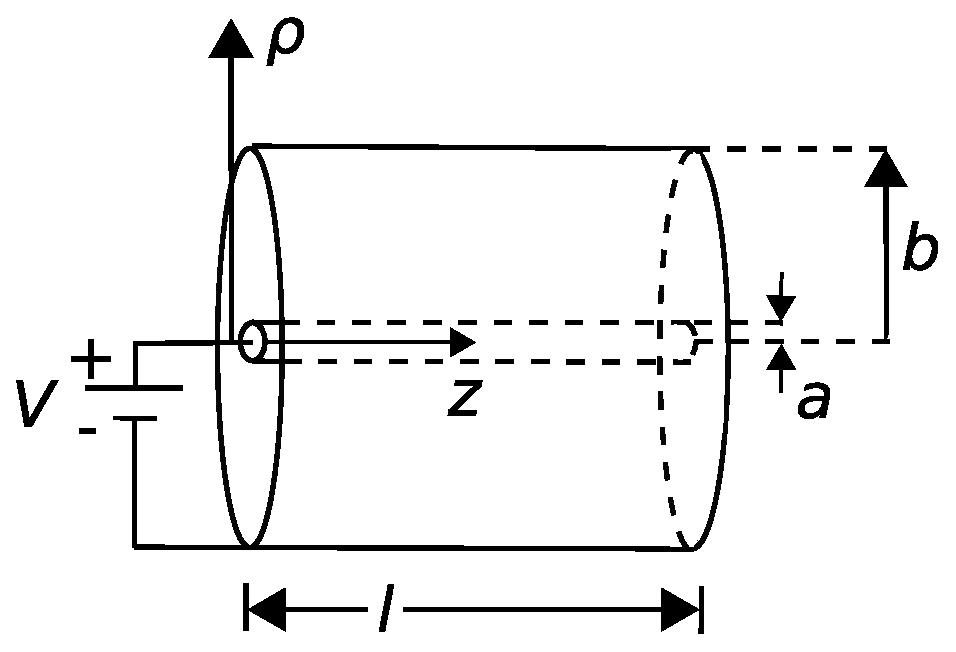
\includegraphics[width=2.5in]{modules/m0113_fCapCoax.eps}
% https://commons.wikimedia.org/wiki/File:M0113_fCapCoax.svg
}}{A three dimensional cylinder with length l and radius b lies on its side with a narrow concentric cylinder through the middle with similar length and radius a. A battery is attached to the interior cylinder by its positive side, and the negative side attached to the exterior cylinder. The vector z is shown pointing to the right from the left edge of the interior cylinder. A vector rho extends up from the point of connection perpendicular to z.}
\end{center} 
\centerline{\scriptsize 
\copyright~\hyperref[m0113_fCapCoax_Credit]{K.\ Kikkeri} 
\href{https://creativecommons.org/licenses/by-sa/4.0/}{CC BY~SA 4.0} 
} 
\caption{
\label{m0113_fCapCoax}
Determining the capacitance of a coaxial structure.
}
\end{figure}

In this section, we shall find the capacitance by assuming a total charge $Q_+$ on the inner conductor and integrating over the associated electric field to obtain the voltage between the conductors.  Then, capacitance is computed as the ratio of the assumed charge to the resulting potential difference.
This strategy is the same as that employed in Section~\ref{m0070_Parallel_Plate_Capacitor_Capacitance_from_Charge} for the parallel plate capacitor, so it may be useful to review that section before attempting this derivation.

The first step is to find the electric field inside the structure.
This is relatively simple if we assume that the structure has infinite length (i.e., $l\to\infty$), since then there are no fringing fields and the internal field will be utterly constant with respect to $z$.
In the central region of a finite-length capacitor, however, the field is not much different from the field that exists in the case of infinite length, and if the energy storage in fringing fields is negligible compared to the energy storage in this central region then there is no harm in assuming the internal field is constant with $z$. 
Alternatively, we may think of the length $l$ as pertaining to one short section of a much longer structure and thereby obtain the capacitance \emph{per length} as opposed to the total capacitance.
Note that the latter is exactly what we need for the transmission line lumped-element equivalent circuit model (Section~\ref{m0029_Lumped-Element_Model}). 

To determine the capacitance, we invoke the definition (Section~\ref{m0112_Capacitance}):
%
\begin{equation}
C \triangleq \frac{Q_+}{V}
\label{m0113_eCapDef}
\end{equation}
%
where $Q_+$ is the charge on the positively-charged conductor and $V$ is the potential measured from the negative conductor to the positive conductor.
The charge on the inner conductor is uniformly-distributed with density 
%
\begin{equation}
\rho_l = \frac{Q_+}{l}
\end{equation}
%
which has units of C/m.
Now we will determine the electric field intensity ${\bf E}$, integrate ${\bf E}$ over a path between conductors to get $V$, and then apply Equation~\ref{m0113_eCapDef} to obtain the capacitance.

The electric field intensity for this scenario was determined in Section~\ref{m0149_E_due_to_Inf_Line_Charge}, ``Electric Field Due to an Infinite Line Charge using Gauss' Law,'' where we found
%
\begin{equation}
{\bf E} = \hat{\rho} \frac{\rho_l}{2\pi \epsilon_s \rho}
\end{equation}
%
The reader should note that in that section we were considering merely a line of charge; not a coaxial structure.
So, on what basis do we claim the field is the same?
This is a consequence of Gauss' Law (Section~\ref{m0014_Gauss_Law_Integral_Form})
%
\begin{equation}
\oint_{\mathcal S} {\bf D}\cdot d{\bf s} = Q_{encl}
\end{equation}
%
which we used in Section~\ref{m0149_E_due_to_Inf_Line_Charge} to find the field.
If in this new problem we specify the same cylindrical surface $\mathcal{S}$ with radius $\rho<b$, then the enclosed charge is the same.
Furthermore, the presence of the outer conductor does not change the radial symmetry of the problem, and nothing else remains that can change the outcome.
This is worth noting for future reference:
%
%ORB HIGHLIGHT
\begin{mdframed}[backgroundcolor=yellow!20,nobreak=true] 
The electric field inside a coaxial structure comprised of concentric conductors and having uniform charge density on the inner conductor is identical to the electric field of a line charge in free space having the same charge density.
\end{mdframed}

Next, we get $V$ using (Section~\ref{m0061_Force_Energy_and_Potential_Difference})
%
\begin{equation}
V = -\int_{\mathcal C}{ {\bf E} \cdot d{\bf l} }
\end{equation}
%
where $\mathcal{C}$ is any path from the negatively-charged outer conductor to the positively-charged inner conductor.
Since this can be \emph{any} such path (Section~\ref{m0062_Independence_of_Path}), we may as well choose the simplest one.
This path is the one that traverses a radial of constant $\phi$ and $z$.
Thus: 
%
\begin{flalign}
V &= -\int_{\rho=b}^a{ \left( \hat{\bf \rho} \frac{\rho_l}{2\pi \epsilon_s \rho} \right) \cdot \left(\hat{\bf \rho}d\rho\right) }  \nonumber \\
  &= - \frac{\rho_l}{2\pi \epsilon_s} \int_{\rho=b}^a{ \frac{d\rho}{\rho}  }  \nonumber \\
  &= + \frac{\rho_l}{2\pi \epsilon_s} \int_{\rho=a}^b{ \frac{d\rho}{\rho}  }  \nonumber \\
  &= + \frac{\rho_l}{2\pi \epsilon_s} \ln\left(\frac{b}{a}\right)
\end{flalign} 

Wrapping up:
%
\begin{equation}
C \triangleq \frac{Q_+}{V} = \frac{\rho_l l}{ \left( \rho_l / 2\pi \epsilon_s \right) \ln\left(b/a\right) }
\end{equation}
%
Note that factors of $\rho_l$ in the numerator and denominator cancel out, leaving:
%
\begin{equation}
\boxed{
C = \frac{2\pi \epsilon_s l}{\ln\left(b/a\right)}   
}
\end{equation}
%
Note that this expression is dimensionally correct, having units of F. 
Also note that the expression depends only on materials (through $\epsilon_s$) and geometry (through $l$, $a$, and $b$).
The expression does \emph{not} depend on charge or voltage, which would imply non-linear behavior.

To make the connection back to lumped-element transmission line model parameters (Sections~\ref{m0029_Lumped-Element_Model} and \ref{m0143_Coaxial_Line}), we simply divide by $l$ to get the per-unit length parameter:
%
\begin{equation}
\boxed{
C' = \frac{2\pi \epsilon_s}{\ln\left(b/a\right)}   
}
\label{m0113_eCp}
\end{equation}

\index{transmission line!coaxial|(}
%ORB EXAMPLE
~\\ \begin{example} 
\begin{mdframed}[backgroundcolor=brown!20,linecolor=brown!20]\raggedright
Capacitance of RG-59 
\index{RG-59}
coaxial cable.
\\~\\
RG-59 coaxial cable consists of an inner conductor having radius $0.292$~mm, an outer conductor having radius $1.855$~mm, and a polyethylene spacing material having relative permittivity 2.25.
Estimate the capacitance per length of RG-59.

{\bf Solution.} 
From the problem statement, 
$a=0.292$~mm, 
$b=1.855$~mm, 
and $\epsilon_s = 2.25\epsilon_0$.
Using Equation~\ref{m0113_eCp} we find $C'=67.7$~pF/m.
\end{mdframed}\end{example}

\index{transmission line!coaxial|)}

      \vfill\break
    \section{Electrostatic Energy}
{\color{blue}\tiny[m0114]}      % This is text associated with the open textbook "Open Electromagnetics"
% See immediately below for author, date
% This work is licensed under the Creative Commons Attribution-ShareAlike 4.0 International License. (CC BY-SA 4.0) 
% To view a copy of the license, visit http://creativecommons.org/licenses/by-sa/4.0/

%ORB TITLE Electrostatic Energy
%ORB AUTHOR 0        # S.W. Ellingson, Virginia Tech (ellingson@vt.edu)
%ORB DATE 20180806   # yyyymmdd
%ORB ABSTRACT Electrostatic Energy

\label{m0114_Electric_Energy} % <-- Must match name of this file and module directory name.  Don't mess with this!
\index{energy!electrostatic|(}

Consider a structure consisting of two perfect conductors, both fixed in position and separated by an ideal dielectric.
This could be a capacitor, 
\index{capacitor!energy storage}
or it could be one of a variety of capacitive structures that are not explicitly intended to be a capacitor -- for example, a printed circuit board.
When a potential difference is applied between the two conducting regions, a positive charge $Q_+$ will appear on the surface of the conductor at the higher potential, and a negative charge $Q_-=-Q_+$ will appear on the surface of the conductor at the lower potential (Section~\ref{m0025_Charge_and_Electric_Field_for_a_Perfectly_Conducting_Region}).
Assuming the conductors are not free to move, potential energy 
\index{energy!potential}
is stored in the electric field associated with the surface charges (Section~\ref{m0112_Capacitance}).

We now ask the question, what is the energy stored in this field? 
The answer to this question has relevance in several engineering applications.
For example, when capacitors are used as batteries, it is useful to know to amount of energy that can be stored.
Also, any system that includes capacitors or has unintended capacitance is using some fraction of the energy delivered by the power supply to charge the associated structures. In many electronic systems -- and in digital systems in particular -- capacitances are periodically charged and subsequently discharged at a regular rate.  Since power is energy per unit time, this cyclic charging and discharging of capacitors consumes power.  Therefore, energy storage in capacitors contributes to the power consumption of modern electronic systems. We'll delve into that topic in more detail in Example~\ref{m0114_eMulticore}.

Since capacitance $C$ relates the charge $Q_+$ to the potential difference $V$ between the conductors, this is the natural place to start.  From the definition of capacitance (Section~\ref{m0112_Capacitance}):
%
\begin{equation}
V = \frac{Q_+}{C} 
\end{equation}
%
From Section~\ref{m0061_Force_Energy_and_Potential_Difference}, electric potential is defined as the work done (i.e., energy injected) by moving a charged particle, per unit of charge; i.e.,
%
\begin{equation}
V = \frac{W_e}{q}
\end{equation}
%
where $q$ is the charge borne by the particle and $W_e$ (units of J) is the work done by moving this particle across the potential difference $V$.
Since we are dealing with charge distributions as opposed to charged particles, it is useful to express this in terms of the contribution $\Delta W_e$ made to $W_e$ by a small charge $\Delta q$. Letting $\Delta q$ approach zero we have
%
\begin{equation}
dW_e = V dq
\end{equation}
%
Now consider what must happen to transition the system from having zero charge ($q=0$) to the fully-charged but static condition ($q=Q_+$). This requires moving the differential amount of charge $dq$ across the potential difference between conductors, beginning with $q=0$ and continuing until $q=Q_+$.
Therefore, the total amount of work done in this process is:
%
\begin{flalign}
W_e &= \int_{q=0}^{Q_+} dW_e \nonumber \\
    &= \int_{0}^{Q_+} V dq  \nonumber \\
    &= \int_{0}^{Q_+} \frac{q}{C}~dq  \nonumber \\
    &= \frac{1}{2}\frac{Q_+^2}{C} 
\label{m0114_eWeQC}
\end{flalign}
%
Equation~\ref{m0114_eWeQC} can be expressed entirely in terms of electrical potential by noting again that $C = Q_+/V$, so
%
\begin{equation}
\boxed{
W_e = \frac{1}{2} CV^2
}
\label{m0114_eESE}
\end{equation}
%
Since there are no other processes to account for the injected energy, the energy stored in the electric field is equal to $W_e$.  Summarizing:
%
%ORB HIGHLIGHT
\begin{mdframed}[backgroundcolor=yellow!20,nobreak=true] 
The energy stored in the electric field of a capacitor (or a capacitive structure) is given by Equation~\ref{m0114_eESE}.
\end{mdframed}

%--------------------------------------------------------

%ORB EXAMPLE
~\\ \begin{example} 
\label{m0114_eMulticore}
\begin{mdframed}[backgroundcolor=brown!20,linecolor=brown!20]\raggedright
Why multicore computing is power-neutral.
\\~\\
Readers are likely aware that computers increasingly use multicore processors as opposed to single-core processors.
For our present purposes, a ``core'' is defined as the smallest combination of circuitry that performs independent computation.
A multicore processor consists of multiple identical cores that run in parallel.
Since a multicore processor consists of $N$ identical processors, you might expect power consumption to increase by $N$ relative to a single-core processor.
However, this is not the case.
To see why, first realize that the power consumption of a modern computing core is dominated by the energy required to continuously charge and discharge the multitude of capacitances within the core.  
From Equation~\ref{m0114_eESE}, the required energy is $\frac{1}{2}C_0V_0^2$ per clock cycle, where $C_0$ is the sum capacitance (remember, capacitors in parallel add) and $V_0$ is the supply voltage. Power is energy per unit time, so the power consumption for a single core is 
%
\begin{equation}
P_0 = \frac{1}{2}C_0V_0^2f_0
\end{equation}
%
where $f_0$ is the clock frequency.
In a $N$-core processor, the sum capacitance is increased by $N$.
However, the frequency is decreased by $N$ since the same amount of computation is (nominally) distributed among the $N$ cores.
Therefore, the power consumed by an $N$-core processor is
%
\begin{equation}
P_N = \frac{1}{2}\left(NC_0\right)V_0^2\left(\frac{f_0}{N}\right) = P_0 
\end{equation}
%
In other words, the increase in power associated with replication of hardware is nominally offset by the decrease in power enabled by reducing the clock rate.
In yet other words, the total energy of the $N$-core processor is $N$ times the energy of the single core processor at any given time; however, the multicore processor needs to recharge capacitances $1/N$ times as often.  

Before moving on, it should be noted that the usual reason for pursuing a multicore design is to increase the amount of computation that can be done; i.e., to increase the product $f_0 N$.   Nevertheless, it is extremely helpful that power consumption is proportional to $f_0$ only, and is independent of $N$.
\end{mdframed}\end{example}

%--------------------------------------------------------

The thin parallel plate capacitor (Section~\ref{m0070_Parallel_Plate_Capacitor_Capacitance_from_Charge}) is representative of a large number of practical applications, so it is instructive to consider the implications of Equation~\ref{m0114_eESE} for this structure in particular.
For the thin parallel plate capacitor,
%
\begin{equation}
C \approx \frac{\epsilon A}{d}
\end{equation}
%
where $A$ is the plate area, $d$ is the separation between the plates, and $\epsilon$ is the permittivity of the material between the plates.
This is an approximation because the fringing field is neglected; we shall proceed as if this is an exact expression.
Applying Equation~\ref{m0114_eESE}:
%
\begin{equation}
W_e = \frac{1}{2} \left(\frac{\epsilon A}{d}\right)\left(Ed\right)^2 
\end{equation}
%
where $E$ is the magnitude of the electric field intensity between the plates.
Rearranging factors, we obtain:
%
\begin{equation}
W_e = \frac{1}{2} \epsilon E^2 \left(A d\right) 
\end{equation}
%
Recall that the electric field intensity in the thin parallel plate capacitor is approximately uniform.
Therefore, the density of energy stored in the capacitor is also approximately uniform.
Noting that the product $Ad$ is the volume of the capacitor, we find that the energy density is
%
\begin{equation}
w_e = \frac{W_e}{Ad} = \frac{1}{2} \epsilon E^2 
\label{m0114_eED}
\end{equation}
%
which has units of energy per unit volume (J/m$^3$).

The above expression provides an alternative method to compute the total electrostatic energy.
Within a mathematical volume ${\mathcal V}$, the total electrostatic energy is simply the integral of the energy density over ${\mathcal V}$; i.e., 
%
\begin{equation}
W_e = \int_{\mathcal V} w_e~dv  
\end{equation}
%
This works even if $E$ and $\epsilon$ vary with position. 
So, even though we arrived at this result using the example of the thin parallel-plate capacitor, our findings at this point apply generally.
Substituting Equation~\ref{m0114_eED} we obtain:
%
\begin{equation}
\boxed{
W_e = \frac{1}{2} \int_{\mathcal V} \epsilon E^2 dv  
}
\label{m0114_eEDV}
\end{equation}
%
Summarizing:
%
%ORB HIGHLIGHT
\begin{mdframed}[backgroundcolor=yellow!20,nobreak=true] 
The energy stored by the electric field present within a volume is given by Equation~\ref{m0114_eEDV}.
\end{mdframed}
%
It's worth noting that this energy increases with the permittivity of the medium, which makes sense since capacitance is proportional to permittivity.

\index{energy!electrostatic|)}


%%%      \vfill\break
{\color{blue}\tiny[m0034]}    % This is text associated with the open textbook "Open Electromagnetics"
% See immediately below for author, date
% This work is licensed under the Creative Commons Attribution-ShareAlike 4.0 International License. (CC BY-SA 4.0) 
% To view a copy of the license, visit http://creativecommons.org/licenses/by-sa/4.0/

%ORB TITLE Image Credits
%ORB AUTHOR 0        # S.W. Ellingson, Virginia Tech (ellingson@vt.edu)
%ORB DATE 20170901   # yyyymmdd
%ORB ABSTRACT End matter for chapter entitled "Electrostatics: Static Charge"

\label{m0034_Ch_End_Matter_Electrostatics_Static_Charge} % <-- Must match name of this file and module directory name.  Don't mess with this!

\onecolumn
\section*{Image Credits}

\begin{itemize}

\item[Fig.] \label{m0102_fCoulombsLaw_Credit}
  \ref{m0102_fCoulombsLaw}:
  \copyright~K.\ Kikkeri, 
  \url{https://commons.wikimedia.org/wiki/File:M0102_fCoulombsLaw.svg},\\ 
  CC BY~SA 4.0 (\url{https://creativecommons.org/licenses/by-sa/4.0/}).

\item[Fig.] \label{m0104_fRing_Credit}
  \ref{m0104_fRing}:
  \copyright~K.\ Kikkeri, 
  \url{https://commons.wikimedia.org/wiki/File:M0104_fRing.svg},\\ 
  CC BY~SA 4.0 (\url{https://creativecommons.org/licenses/by-sa/4.0/}).

\item[Fig.] \label{m0104_fDisk_Credit}
  \ref{m0104_fDisk}:
  \copyright~K.\ Kikkeri, 
  \url{https://commons.wikimedia.org/wiki/File:M0104_fDisk.svg},\\ 
  CC BY~SA 4.0 (\url{https://creativecommons.org/licenses/by-sa/4.0/}).

\item[Fig.] \label{m0149_fGLLS_Credit}
  \ref{m0149_fGLLS}:
  \copyright~K.\ Kikkeri, 
  \url{https://commons.wikimedia.org/wiki/File:4.5_m0149_commons.svg},\\ 
  CC BY~SA 4.0 (\url{https://creativecommons.org/licenses/by-sa/4.0/}).

\item[Fig.] \label{m0064_fResistor_Credit}
  \ref{m0064_fResistor}:
  \copyright~K.\ Kikkeri, 
  \url{https://commons.wikimedia.org/wiki/File:M0064_fResistor.svg},\\ 
  CC BY~SA 4.0 (\url{https://creativecommons.org/licenses/by-sa/4.0/}).

\item[Fig.] \label{m0020_fPEC_Credit}
  \ref{m0020_fPEC}:
  \copyright~K.\ Kikkeri, 
  \url{https://commons.wikimedia.org/wiki/File:M0020_fPEC.svg},\\ 
  CC BY~SA 4.0 (\url{https://creativecommons.org/licenses/by-sa/4.0/}).

\item[Fig.] \label{m0020_fKVL_Credit}
  \ref{m0020_fKVL}:
  \copyright~K.\ Kikkeri, 
  \url{https://commons.wikimedia.org/wiki/File:M0020_fKVL.svg},\\ 
  CC BY~SA 4.0 (\url{https://creativecommons.org/licenses/by-sa/4.0/}).

\item[Fig.] \label{m0021_fPEC_Credit}
  \ref{m0021_fPEC}:
  \copyright~K.\ Kikkeri, 
  \url{https://commons.wikimedia.org/wiki/File:M0021_fPEC.svg},\\ 
  CC BY~SA 4.0 (\url{https://creativecommons.org/licenses/by-sa/4.0/}).

\item[Fig.] \label{m0021_fGL_Credit}
  \ref{m0021_fGL}:
  \copyright~K.\ Kikkeri, 
  \url{https://commons.wikimedia.org/wiki/File:M0021_fGL.svg},\\ 
  CC BY~SA 4.0 (\url{https://creativecommons.org/licenses/by-sa/4.0/}).

\item[Fig.] \label{m0025_fFlatSlab_Credit}
  \ref{m0025_fFlatSlab}:
  \copyright~K.\ Kikkeri, 
  \url{https://commons.wikimedia.org/wiki/File:M0025_fFlatSlab.svg},\\ 
  CC BY~SA 4.0 (\url{https://creativecommons.org/licenses/by-sa/4.0/}).

\item[Fig.] \label{m0025_fPEC_field_lines_Credit}
  \ref{m0025_fPEC_field_lines}:
  by~C.\ Burks, 
  \url{https://commons.wikimedia.org/wiki/File:Electrostatic_induction.svg},\\ 
  in public domain. 
  Minor modifications.

%\item[Fig.] \label{m0070_fPPCap_Credit}
%  \ref{m0070_fPPCap}:
%  by inductiveload, 
%  \url{https://en.wikipedia.org/wiki/File:Parallel_plate_capacitor.svg},\\ 
%  public domain.  Modified by author.

\item[Fig.] \label{m0113_fCapCoax_Credit}
  \ref{m0113_fCapCoax}:
  \copyright~K.\ Kikkeri, 
  \url{https://commons.wikimedia.org/wiki/File:M0113_fCapCoax.svg},\\ 
  CC BY~SA 4.0 (\url{https://creativecommons.org/licenses/by-sa/4.0/}).

\end{itemize}

\twocolumn

  \chapter{Steady Current and Conductivity}
  \thispagestyle{fancy} % override footer in first page of chapter
  \fancyhf{}            % reset header and footer
  \fancyfoot[C]{\footnotesize \emph{Electromagnetics Vol~1}. ~\copyright~2018 S.W.\ Ellingson ~CC~BY~SA~4.0. ~\url{https://doi.org/10.21061/electromagnetics-vol-1}}
    \section{Convection and Conduction Currents}
{\color{blue}\tiny[m0110]}      % This is text associated with the open textbook "Open Electromagnetics"
% See immediately below for author, date
% This work is licensed under the Creative Commons Attribution-ShareAlike 4.0 International License. (CC BY-SA 4.0) 
% To view a copy of the license, visit http://creativecommons.org/licenses/by-sa/4.0/

%ORB TITLE Convection and Conduction Currents
%ORB AUTHOR 0        # S.W. Ellingson, Virginia Tech (ellingson@vt.edu)
%ORB DATE 20180806   # yyyymmdd
%ORB ABSTRACT Current Distributions 

\label{m0110_Convection_and_Conduction} % <-- Must match name of this file and module directory name.  Don't mess with this!

In practice, we deal with two physical mechanisms for current: convection and conduction.  
The distinction between these types of current is important in electromagnetic analysis. 

{\bf Convection current} 
\index{current!convection}
consists of charged particles moving in response to mechanical forces, as opposed to being guided by the electric field (Sections~\ref{m0002_Electric_Field_Intensity} and/or \ref{m0102_Coulombs_Law}).  An example of a convection current is a cloud bearing free electrons that moves through the atmosphere driven by wind.

{\bf Conduction current} 
\index{current!conduction}
consists of charged particles moving in response to the electric field and not merely being carried by motion of the surrounding material.  
In some materials, the electric field is also able to dislodge weakly-bound electrons from atoms, which then subsequently travel some distance before reassociating with other atoms.  
For this reason, the individual electrons in a conduction current do not necessarily travel the full distance over which the current is perceived to exist. 

The distinction between convection and conduction is important because \emph{Ohm's Law} 
\index{Ohm's law}
(Section~\ref{m0010_Conductivity}) -- which specifies the relationship between electric field intensity and current -- applies only to conduction current.

%%%%%%%%%%%%%%%%%%%%%%%%%%%%%%%%%%%%%%%%%%%%%%%%%%%%%%%%%%%

{\bf Additional Reading:}
\begin{itemize}
\item ``\href{https://en.wikipedia.org/wiki/Electric_current}{Electric current}'' on Wikipedia.
\end{itemize}









      \vfill\break
    \section{Current Distributions}
{\color{blue}\tiny[m0101]}      % This is text associated with the open textbook "Open Electromagnetics"
% See immediately below for author, date
% This work is licensed under the Creative Commons Attribution-ShareAlike 4.0 International License. (CC BY-SA 4.0) 
% To view a copy of the license, visit http://creativecommons.org/licenses/by-sa/4.0/

%ORB TITLE Current Distributions
%ORB AUTHOR 0        # S.W. Ellingson, Virginia Tech (ellingson@vt.edu)
%ORB DATE 20180806   # yyyymmdd
%ORB ABSTRACT Current Distributions 

\label{m0101_Current_Distributions} % <-- Must match name of this file and module directory name.  Don't mess with this!
\index{current density|(}

In elementary electric circuit theory, current is the rate at which electric charge passes a particular point in a circuit. For example, 1~A is 1~C per second.
In this view current is a scalar quantity, and there are only two possible directions because charge is constrained to flow along defined channels.
Direction is identified by the sign of the current with respect to a reference direction, which is in turn defined with respect to a reference voltage polarity.
The convention in electrical engineering defines positive current as the flow of positive charge into the positive voltage terminal of a passive device such as a resistor, capacitor, or inductor.
For an active device such as a battery, positive current corresponds to the flow of positive charge \emph{out of} the positive voltage terminal.

However, this kind of thinking only holds up when the systems being considered are well-described as ``lumped'' devices connected by infinitesimally thin, filament-like connections representing wires and circuit board traces.
Many important problems in electrical engineering concern situations in which the flow of current is not limited in this way. Examples include wire- and pin-type interconnects at radio frequencies, circuit board and enclosure grounding, and physical phenomena such as lightning.
To accommodate the more general class of problems, we must define current as a vector quantity.
Furthermore, current in these problems can spread out over surfaces and within volumes, so we must also consider \emph{spatial distributions} of current.  

{\bf Line Current.}
\index{current density!line}
As noted above, if a current $I$ is constrained to follow a particular path, then the only other consideration is direction.  Thus, a line current is specified mathematically as $\hat{\bf l}I$, where the direction $\hat{\bf l}$ may vary with position along the path.
For example, in a straight wire $\hat{\bf l}$ is constant, whereas in a coil $\hat{\bf l}$ varies with position along the coil.

{\bf Surface Current Distribution.} 
\index{current density!surface}
In some cases, current may be distributed over a surface.
For example, the radio-frequency current on a wire of radius $a$ made from a metal with sufficiently high conductivity can be modeled as a uniform surface current existing on the wire surface.  
In this case, the current is best described as a surface current density ${\bf J}_s$, which is the total current $I$ on the wire divided by the circumference $2\pi a$ of the wire:
%
\begin{equation}
{\bf J}_s = \hat{\bf u}\frac{I}{2\pi a}~~\mbox{(units of A/m)}
\end{equation} 
%
where $\hat{\bf u}$ is the direction of current flow. 

{\bf Volume Current Distribution.} 
\index{current density!volume}
Imagine that current is distributed within a volume.   
Let $\hat{\bf u}\Delta i$ be the current passing through a small open planar surface defined within this volume, and let $\Delta s$ be the area of this surface.
The \emph{volume current density} ${\bf J}$ at any point in the volume is defined as
%
\begin{equation}
{\bf J} \triangleq \lim_{\Delta s \to 0} \frac{\hat{\bf u}\Delta i}{\Delta s} = \hat{\bf u}\frac{di}{ds}~~\mbox{(units of A/m$^2$)}
\end{equation}
%
In general, ${\bf J}$ is a function of position within this volume.
Subsequently the total current passing through a surface ${\mathcal S}$ is
%
\begin{equation}
I = \int_{\mathcal S} {\bf J}\cdot~d{\bf s}~~\mbox{(units of A)}
\end{equation}
%
In other words, volume current density integrated over a surface yields total current through that surface.  
You might recognize this as a calculation of flux, 
\index{flux}
and it is.\footnote{However, it is not common to refer to net current as a flux; go figure!}

%----------------------------------------------------------

%ORB EXAMPLE
~\\ \begin{example} 
\begin{mdframed}[backgroundcolor=brown!20,linecolor=brown!20]\raggedright
Current and current density in a wire of circular cross-section.
\\~\\
Figure~\ref{m0101_fMatEx1} shows a straight wire having cross-sectional radius $a=3$~mm.  A battery is connected across the two ends of the wire 
resulting in a volume current density ${\bf J} = \hat{\bf z}8$~A/m$^2$, which is uniform throughout the wire.  Find the net current $I$ through the wire.

{\bf Solution.} 
The net current is 
%
\begin{flalign}
I &= \int_{\mathcal{S}} {\bf J} \cdot d{\bf s} \nonumber
\end{flalign}
%
We choose $\mathcal{S}$ to be the cross-section perpendicular to the axis of the wire. 
Also, we choose $d{\bf s}$ to point such that $I$ is positive with respect to the sign convention shown in Figure~\ref{m0101_fMatEx1}  , which is the usual choice in electric circuit analysis.
With these choices, we have
%
\begin{flalign}
I &= \int_{\rho=0}^a\int_{\phi=0}^{2\pi} \left( \hat{\bf z}8~\mbox{A/m}^2 \right) \cdot \left( \hat{\bf z}\rho~d\rho~d\phi \right) \nonumber \\
  &= \left(8~\mbox{A/m}^2 \right) \int_{\rho=0}^a\int_{\phi=0}^{2\pi} \rho~d\rho~d\phi \nonumber \\
  &= \left(8~\mbox{A/m}^2 \right) \cdot \left( \pi a^2 \right) \nonumber \\
  &= 226~\mu\mbox{A} \nonumber
\end{flalign}     
%
This answer is independent of the cross-sectional surface $\mathcal{S}$ used to do the calculation.  For example, you could use an alternative surface that is tilted $45^{\circ}$ away from the axis of the wire. In that case, the cross-sectional area would increase, but the dot product of ${\bf J}$ and $d{\bf s}$ would be proportionally less and the outcome would be the same.  Since the choice of $\mathcal{S}$ is arbitrary -- any surface with edges at the perimeter of the wire will do -- you should make the choice that makes the problem as simple as possible, as we have done above.

\end{mdframed}
%
\begin{figure}
\begin{center}
\pdftooltip{{  % note double braces
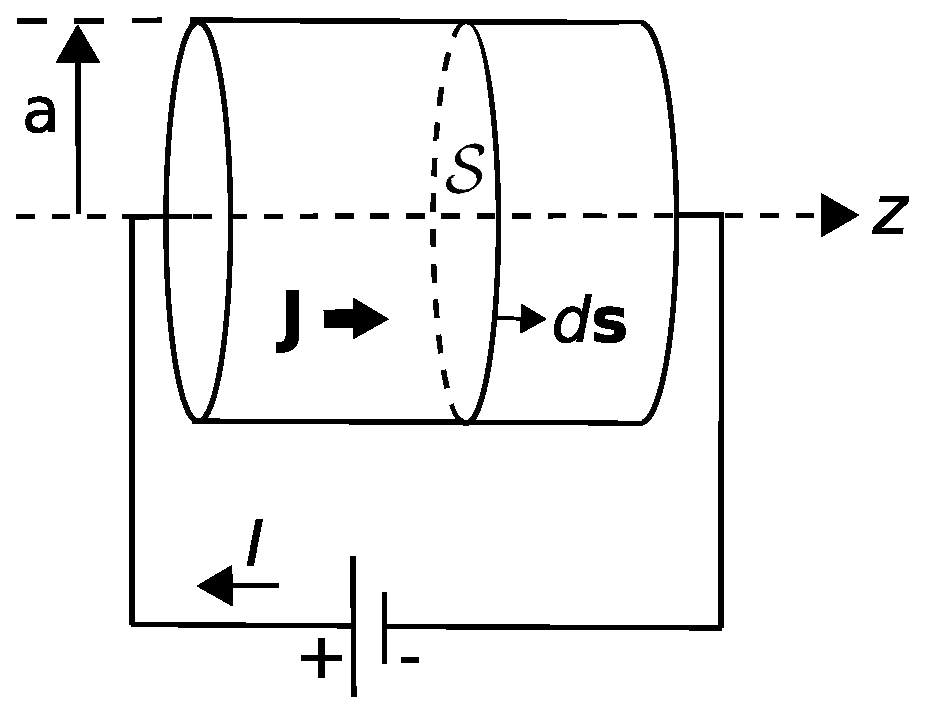
\includegraphics[width=2in]{modules/m0101_fMatEx1.eps}
% https://commons.wikimedia.org/wiki/File:M0101_fMatEx1.svg
}}{A three dimensional section of wire with radius a lies on its side centered on the z-axis. It is connected to a battery, with the positive end connected at the left side and the negative end connected at the right side of the cylinder. A cross-section is labeled S. From the cross-section extends a vector d bold s. Current shown flowing clockwise and current density shown going left to right through the cylinder.}
\end{center} 
\centerline{\scriptsize 
\copyright~\hyperref[m0101_fMatEx1_Credit]{K.\ Kikkeri} 
\href{https://creativecommons.org/licenses/by-sa/4.0/}{CC BY~SA 4.0} 
} 
\caption{
\label{m0101_fMatEx1}
Net current $I$ and current density ${\bf J}$ in a wire of circular cross-section. 
}
\end{figure}
\end{example}

%%%%%%%%%%%%%%%%%%%%%%%%%%%%%%%%%%%%%%%%%%%%%%%%%%%%%%%%%%%

{\bf Additional Reading:}
\begin{itemize}
\item ``\href{https://en.wikipedia.org/wiki/Electric_current}{Electric current}'' on Wikipedia.
\item ``\href{https://en.wikipedia.org/wiki/Current_density}{Current density}'' on Wikipedia.
\end{itemize}

\index{current density|)}








      \vfill\break
    \section{Conductivity}
{\color{blue}\tiny[m0010]}      % This is text associated with the open textbook "Open Electromagnetics"
% See immediately below for author, date
% This work is licensed under the Creative Commons Attribution-ShareAlike 4.0 International License. (CC BY-SA 4.0) 
% To view a copy of the license, visit http://creativecommons.org/licenses/by-sa/4.0/

%ORB TITLE Conductivity
%ORB AUTHOR 0        # S.W. Ellingson, Virginia Tech (ellingson@vt.edu)
%ORB DATE 20180806   # yyyymmdd
%ORB ABSTRACT Conductivity

\label{m0010_Conductivity} % <-- Must match name of this file and module directory name.  Don't mess with this!
\index{conductivity|(}

Conductivity is one of the three primary ``constitutive parameters'' that is commonly used to characterize the electromagnetic properties of materials (Section~\ref{m0007_Properties_of_Materials}).  The key idea is this:

%ORB HIGHLIGHT
\begin{mdframed}[backgroundcolor=yellow!20,nobreak=true] 
Conductivity 
\index{conductivity!definition}
is a property of materials that determines conduction current density in response to an applied electric field.
\end{mdframed}
%
Recall that conduction current is the flow of charge in response to an electric field (Section~\ref{m0110_Convection_and_Conduction}).
Although the associated force is straightforward to calculate (e.g., Section~\ref{m0102_Coulombs_Law}), the result is merely the force applied, not the speed at which charge moves in response.  The latter is determined by the \emph{mobility of charge}, 
\index{charge mobility}
which is in turn determined by the atomic and molecular structure of the material.  
Conductivity relates current density to the applied field directly, without requiring one to grapple separately with the issues of applied force and charge mobility.

In the absence of material -- that is, in a true, perfect vacuum -- conductivity is zero because there is no charge available to form current, and therefore the current is zero no matter what electric field is applied.   
At the other extreme, a \emph{good conductor} 
\index{conductor!good}
is a material that contains a supply of charge that is able to move freely within the material.  
When an electric field is applied to a good conductor, charge-bearing material constituents move in the direction determined by the electric field, creating current flow in that direction.  
This relationship is summarized by \emph{Ohm's Law for Electromagnetics}:
\index{Ohm's law}
%
\begin{equation}
\boxed{
{\bf J} = \sigma {\bf E}
}
\label{m0010_eMatOhmsLaw}
\end{equation}
%
where 
${\bf E}$ is electric field intensity (V/m);
\index{electric field intensity!related to current}
${\bf J}$ is the volume current density, a vector describing the current flow, having units of A/m$^2$ (see Section~\ref{m0101_Current_Distributions}); and
$\sigma$ is conductivity.
Since ${\bf E}$ has units of V/m, we see $\sigma$ has units of $\Omega^{-1}\mbox{m}^{-1}$, which is more commonly expressed as S/m, where 1~S (``siemens'') is defined as $1~\Omega^{-1}$.  
Section~\ref{m0137_Table_of_Conductivities} provides values of conductivity for a representative set of materials. 
%
%ORB HIGHLIGHT
\begin{mdframed}[backgroundcolor=yellow!20,nobreak=true] 
Conductivity $\sigma$ is expressed in units of S/m, where 1~S $=$ 1~$\Omega^{-1}$.  
\end{mdframed}
%
It is important to note that the current being addressed here is \emph{conduction current}, and not convection current, displacement current, or some other form of current -- see Section~\ref{m0101_Current_Distributions} for elaboration.  Summarizing:
%
%ORB HIGHLIGHT
\begin{mdframed}[backgroundcolor=yellow!20,nobreak=true] 
Ohm's Law for Electromagnetics (Equation~\ref{m0010_eMatOhmsLaw}) states that volume density of conduction current (A/m$^2$) equals conductivity (S/m) times electric field intensity (V/m). 
\end{mdframed}

The reader is likely aware that there is also an ``Ohm's Law'' in electric circuit theory, which states that current $I$ (units of A) is voltage $V$ (units of V) divided by resistance $R$ (units of $\Omega$); i.e., $I=V/R$.  This is in fact a special case of Equation~\ref{m0010_eMatOhmsLaw}; see Section~\ref{m0071_Resistance_DC} for more about this. 

As mentioned above, $\sigma$ depends on both the \emph{availability} and \emph{mobility} of charge within the material.  
At the two extremes, we have \emph{perfect insulators}, 
\index{insulator!perfect}
for which $\sigma=0$, and \emph{perfect conductors}, 
\index{conductor!perfect}
for which $\sigma \to \infty$.  
Some materials approach these extremes, whereas others fall midway between these conditions.  
Here are a few classes of materials that are frequently encountered:
%
\begin{itemize}

\item A perfect vacuum -- ``free space'' -- contains no charge and therefore is a perfect insulator with $\sigma=0$. 

\item \emph{Good insulators} typically have conductivities $\ll 10^{-10}$~S/m, which is sufficiently low that the resulting currents can usually be ignored.  The most important example is air, which has a conductivity only slightly greater than that of free space.  An important class of good insulators is {\it lossless dielectrics},\footnote{See Section~\ref{m0107_Dielectric_Media} 
\index{dielectric (material)!lossless}
for a discussion of dielectric materials.} which are well-characterized in terms of permittivity
\index{permittivity}
($\epsilon$) alone, and for which $\mu=\mu_0$ and $\sigma=0$ may usually be assumed. 

\item \emph{Poor insulators} 
\index{insulator!poor}
have conductivities that are low, but nevertheless sufficiently high that the resulting currents cannot be ignored.  For example, the dielectric material that is used to separate the conductors in a transmission line must be considered a poor insulator as opposed to a good (effectively lossless) insulator in order to characterize loss per length along the transmission line, which can be significant.\footnote{Review Sections~\ref{m0029_Lumped-Element_Model}, \ref{m0083_Lossless_Transmission_Lines}, and associated sections for a refresher on this issue.}
These \emph{lossy dielectrics} 
\index{dielectric (material)!lossy}
are well-characterized in terms of $\epsilon$ and $\sigma$, and typically $\mu=\mu_0$ can be assumed. 

\item \emph{Semiconductors} 
\index{semiconductor (material)}
such as those materials used in integrated circuits have intermediate conductivities, typically in the range $10^{-4}$ to $10^{+1}$~S/m.

\item \emph{Good conductors} 
\index{conductor!good}
are materials with very high conductivities, typically greater than $10^5$~S/m.  
An important category of good conductors includes metals, with certain metals including alloys of aluminum, copper, and gold reaching conductivities on the order of $10^8$~S/m. 
In such materials, minuscule electric fields give rise to large currents.   
There is no significant storage of energy in such materials, and so the concept of permittivity is not relevant for good conductors. 

\end{itemize}

The reader should take care to note that terms such as {\it good conductor} and {\it poor insulator} are qualitative and subject to context.  What may be considered a ``good insulator'' in one application may be considered to be a ``poor insulator'' in another.  

One relevant category of material was not included in the above list -- namely, \emph{perfect conductors}. 
A perfect conductor is a material in which $\sigma\to\infty$.  
It is tempting to interpret this as meaning that any electric field gives rise to infinite current density; however, this is not plausible even in the ideal limit.
Instead, this condition is interpreted as meaning that ${\bf E}={\bf J}/\sigma\to 0$ throughout the material; i.e., ${\bf E}$ is zero independently of any current flow in the material.
An important consequence is that the potential field $V$ is equal to a constant value throughout the material.  
(Recall ${\bf E}=-\nabla V$ (Section~\ref{m0063_Electric_Field_as_the_Gradient_of_Potential}), so constant $V$ means ${\bf E}=0$.)
We refer to the volume occupied by such a material as an \emph{equipotential volume}.
This concept is useful as an approximation of the behavior of good conductors; for example, metals are often modeled as perfectly-conducting equipotential volumes in order to simplify analysis.
%
%ORB HIGHLIGHT
\begin{mdframed}[backgroundcolor=yellow!20,nobreak=true] 
A perfect conductor 
\index{conductor!perfect (definition)}
is a material for which $\sigma\to\infty$, ${\bf E}\to 0$, and subsequently $V$ (the electric potential) is constant.  
\end{mdframed}

One final note: It is important to remain aware of the assumptions we have made about materials in this book, which are summarized in Section~\ref{m0007_Properties_of_Materials}. In particular, we continue to assume that materials are linear unless otherwise indicated.  
For example, whereas air is normally considered to be a good insulator and therefore a poor conductor, anyone who has ever witnessed lightning 
\index{lightning}
has seen a demonstration that under the right conditions -- i.e., sufficiently large potential difference between earth and sky -- current will readily flow through air.  This particular situation is known as \emph{dielectric breakdown} 
\index{dielectric breakdown}
(see Section~\ref{m0109_Dielectric_Breakdown}).  The non-linearity of materials can become evident before reaching the point of dielectric breakdown, so one must be careful to consider this possibility when dealing with strong electric fields.

{\bf Additional Reading:}
\begin{itemize}
\item ``\href{https://en.wikipedia.org/wiki/Electrical_resistivity_and_conductivity}{Electrical Resistivity and Conductivity}'' on Wikipedia.
\item ``\href{https://en.wikipedia.org/wiki/Ohm's_law}{Ohm's Law}'' on Wikipedia.
\end{itemize}

\index{conductivity|)}

      \vfill\break
    \section{Resistance}
{\color{blue}\tiny[m0071]}      % This is text associated with the open textbook "Open Electromagnetics"
% See immediately below for author, date
% This work is licensed under the Creative Commons Attribution-ShareAlike 4.0 International License. (CC BY-SA 4.0) 
% To view a copy of the license, visit http://creativecommons.org/licenses/by-sa/4.0/

%ORB TITLE Resistance
%ORB AUTHOR 0        # S.W. Ellingson, Virginia Tech (ellingson@vt.edu)
%ORB DATE 20180806   # yyyymmdd
%ORB ABSTRACT Resistance at DC

\label{m0071_Resistance_DC} % <-- Must match name of this file and module directory name.  Don't mess with this!
\index{resistance|(}

The concept of resistance is most likely familiar to readers via \emph{Ohm's Law for Devices}; i.e., $V=IR$ where $V$ is the potential difference associated with a current $I$.
This is correct, but it is not the whole story. 
Let's begin with a statement of intent:
%
%ORB HIGHLIGHT
\begin{mdframed}[backgroundcolor=yellow!20,nobreak=true] 
Resistance 
\index{resistance!definition}
$R$ ($\Omega$) is a characterization of the conductivity of a \emph{device} (as opposed to a \emph{material}) in terms of Ohms Law for Devices; i.e., $V=IR$.
\end{mdframed}
%
Resistance is a property of devices such as resistors, which are intended to provide resistance, as well as being a property of most practical electronic devices, whether it is desired or not.  

Resistance is a manifestation of the conductivity of the materials comprising the device, which subsequently leads to the ``$V=IR$'' relationship.  This brings us to a very important point and a common source of confusion.
\emph{Resistance is not necessarily the real part of impedance.}
\index{impedance!of resistance}
Let's take a moment to elaborate.
Impedance ($Z$) is defined as the ratio of voltage to current; i.e., $V/I$; or equivalently in the phasor domain as $\widetilde{V}/\widetilde{I}$.
Most devices -- not just devices exhibiting resistance -- can be characterized in terms of this ratio.
Consider for example the input impedance of a terminated transmission line (Section~\ref{m0087_Input_Impedance_of_a_Terminated_Lossless_Transmission_Line}).  This impedance may have a non-zero real-valued component even when the transmission line and the terminating load are comprised of perfect conductors.
Summarizing:
%ORB HIGHLIGHT
\begin{mdframed}[backgroundcolor=yellow!20,nobreak=true] 
Resistance results in a real-valued impedance. However, not all devices exhibiting a real-valued impedance exhibit resistance.  Furthermore, the real component of a complex-valued impedance does not necessarily represent resistance. 
\end{mdframed}
%
Restating the main point in yet other words: \emph{Resistance pertains to limited conductivity, not simply to voltage-current ratio.}

Also important to realize is that 
whereas conductivity 
\index{conductivity}
$\sigma$ (units of S/m) is a property of materials,
resistance depends on \emph{both} conductivity and the geometry of the device. 
In this section, we address the question of how the resistance of a device can be is determined.
The following example serves this purpose.

\index{resistance!of wire (DC)|(}
\index{wire!DC resistance of|(}

Figure~\ref{m0071_fMatEx1} shows a straight wire 
of length $l$ centered on the $z$ axis, forming a cylinder of material having conductivity $\sigma$ and cross-sectional radius $a$.  
The ends of the cylinder are covered by perfectly-conducting plates to which the terminals are attached.
A battery is connected to the terminals, resulting in a uniform internal electric field ${\bf E}$ between the plates.  
%
\begin{figure}
\begin{center}
\pdftooltip{{  % note double braces
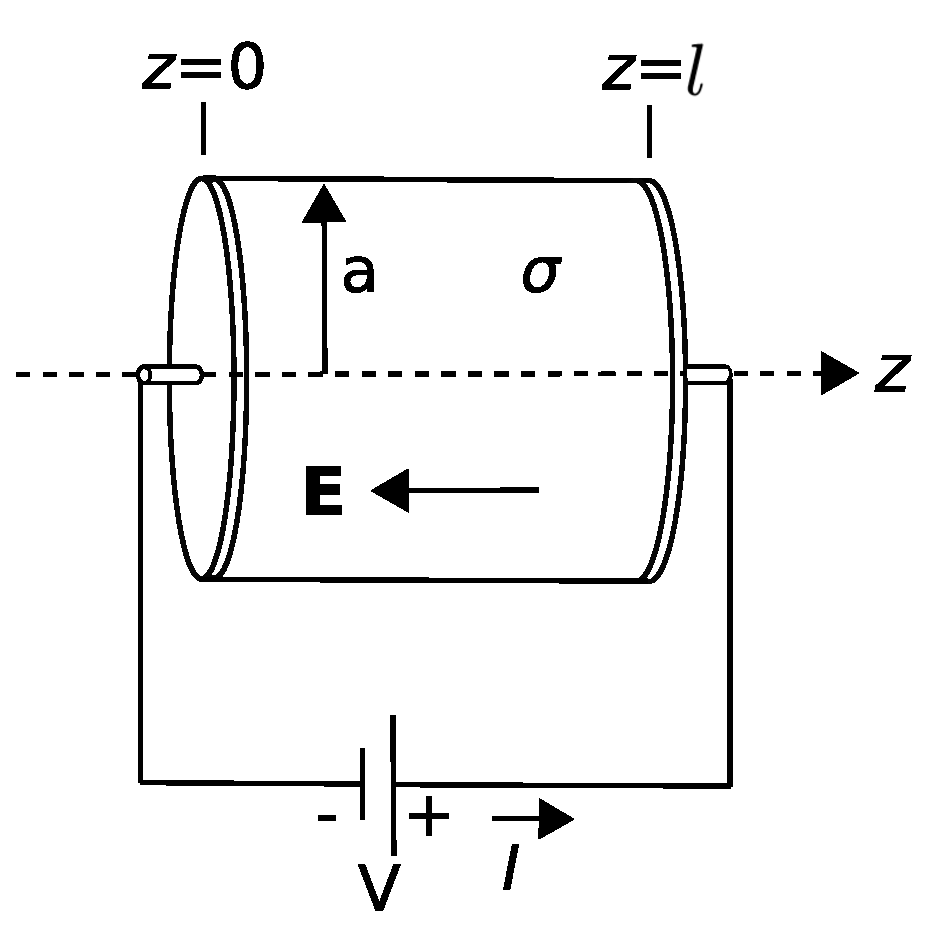
\includegraphics[width=2in]{modules/m0071_fMatEx1.eps}
% https://commons.wikimedia.org/wiki/File:M0071_fMatEx1.svg
}}{A three-dimensional wire with radius a, length l, and conductivity sigma lies on its side centered on the z-axis. On both ends of the wire are two thin plates, with terminals on each side. The left plate is labeled z = 0, and the right plate is labeled z = l. The wire is connected to a battery, with the positive side connected to the right side of the wire with current flowing counterclockwise. The internal electric field in the wire is represented by a vector pointed to the left, labeled E.}
\end{center} 
\centerline{\scriptsize 
\copyright~\hyperref[m0071_fMatEx1_Credit]{K.\ Kikkeri} 
\href{https://creativecommons.org/licenses/by-sa/4.0/}{CC BY~SA 4.0} 
} 
\caption{
\label{m0071_fMatEx1}
Analysis of the resistance of straight wire of circular cross-section. 
}
\end{figure}

To calculate $R$ for this device, let us first calculate $V$, then $I$, and finally $R=V/I$.  
First, we compute the potential difference using the following result from Section~\ref{m0061_Force_Energy_and_Potential_Difference}:
%
\begin{equation}
V = -\int_{\mathcal C}{\bf E}\cdot d{\bf l}
\end{equation}
%
Here we can view $V$ as a ``given'' (being the voltage of the battery), but wish to evaluate the right hand side so as to learn something about the effect of the conductivity and geometry of the wire.
The appropriate choice of ${\mathcal C}$ begins at $z=0$ and ends at $z=l$, following the axis of the cylinder.
(Remember: ${\mathcal C}$ defines the reference direction for increasing potential, so the resulting potential difference will be the node voltage at the end point minus the node voltage at the start point.)
Thus, $d{\bf l} = \hat{\bf z}dz$ and we have
%
\begin{flalign}
V &= -\int_{z=0}^{l} {\bf E} \cdot \left(\hat{\bf z}dz\right) \nonumber
\end{flalign} 
%
We do not yet know ${\bf E}$; however, we know it is constant throughout the device and points in the $-\hat{\bf z}$ direction since this is the direction of current flow and Ohm's Law for Electromagnetics (Section~\ref{m0010_Conductivity}) requires the electric field to point in the same direction.
Thus, we may write ${\bf E}=-\hat{\bf z}E_z$ where $E_z$ is a constant.
We now find:
%
\begin{flalign}
V &= -\int_{z=0}^{l} \left(-\hat{\bf z}E_z\right) \cdot \left(\hat{\bf z}dz\right) \nonumber \\
  &= +E_z \int_{z=0}^{l} dz \nonumber \\
  &= +E_z l \nonumber
\end{flalign} 

The current $I$ is given by (Section~\ref{m0101_Current_Distributions})
%
\begin{flalign}
I &= \int_{\mathcal{S}} {\bf J} \cdot d{\bf s} \nonumber
\end{flalign}
%
We choose the surface $\mathcal{S}$ to be the cross-section perpendicular to the axis of the wire. 
Also, we choose $d{\bf s}$ to point such that $I$ is positive with respect to the sign convention shown in Figure~\ref{m0071_fMatEx1}.
With these choices, we have
%
\begin{flalign}
I &= \int_{\rho=0}^a\int_{\phi=0}^{2\pi} {\bf J} \cdot \left( -\hat{\bf z}~\rho~d\rho~d\phi \right) \nonumber
\end{flalign}
%
From Ohm's Law for Electromagnetics, we have
%
\begin{equation}
{\bf J} = \sigma{\bf E} = -\hat{\bf z} \sigma E_z
\end{equation}
%
So now
%
\begin{flalign}
I &= \int_{\rho=0}^a\int_{\phi=0}^{2\pi} \left( -\hat{\bf z} \sigma E_z  \right) \cdot \left(-\hat{\bf z}\rho~d\rho~d\phi \right) \nonumber \\
  &= \sigma E_z \int_{\rho=0}^a\int_{\phi=0}^{2\pi} \rho~d\rho~d\phi \nonumber \\
  &= \sigma E_z \left( \pi a^2 \right) \nonumber
\end{flalign}     
%
Finally:
%
\begin{equation}
R = \frac{V}{I} 
  = \frac{E_z l}{\sigma E_z \left( \pi a^2 \right)} 
  = \frac{l}{\sigma \left( \pi a^2 \right)} \nonumber 
\end{equation}
%
This is a good-enough answer for the problem posed, but it is easily generalized a bit further.  Noting that $\pi a^2$ in the denominator is the cross-sectional area $A$ of the wire, so we find:
%
\begin{equation}
\boxed{
R = \frac{l}{\sigma A}
}
\label{m0071_eRwireDC}
\end{equation}
%
i.e., the resistance of a wire having cross-sectional area $A$ -- regardless of the shape of the cross-section, is given by the above equation.
%
%ORB HIGHLIGHT
\begin{mdframed}[backgroundcolor=yellow!20,nobreak=true] 
The resistance of a right cylinder of material, given by Equation~\ref{m0071_eRwireDC}, is proportional to length and inversely proportional to cross-sectional area and conductivity.
\end{mdframed}

It is important to remember that Equation~\ref{m0071_eRwireDC} presumes that the volume current density ${\bf J}$ is uniform over the cross-section of the wire.  
This is an excellent approximation for thin wires at ``low'' frequencies including, of course, DC.
At higher frequencies it may not be a good assumption that ${\bf J}$ is uniformly-distributed over the cross-section of the wire, and at sufficiently high frequencies one finds instead that the current is effectively limited to the exterior surface of the wire.  
In the ``high frequency'' case, $A$ in Equation~\ref{m0071_eRwireDC} is reduced from the physical area to a smaller value corresponding to the reduced area through which most of the current flows.
Therefore, $R$ increases with increasing frequency.  
To quantify the high frequency behavior of $R$ (including determination of what constitutes ``high frequency'' in this context) one requires concepts beyond the theory of electrostatics, so this is addressed elsewhere.

%----------------------------------------------------------

%ORB EXAMPLE
~\\ \begin{example} 
\begin{mdframed}[backgroundcolor=brown!20,linecolor=brown!20]\raggedright
Resistance of 22~AWG hookup wire.
\\~\\
A common type of wire found in DC applications is 22AWG (``American Wire Gauge''; see ``Additional Resources'' at the end of this section) copper solid-conductor hookup wire.
This type of wire has circular cross-section with diameter 0.644~mm.
What is the resistance of 3~m of this wire? 
Assume copper conductivity of $58$~MS/m.

{\bf Solution.} 
From the problem statement,
the diameter $2a=0.644$~mm,
$\sigma=58\times 10^6$~S/m, and 
$l=3$~m.
The cross-sectional area is $A=\pi a^2 \cong 3.26\times10^{-7}$~m$^2$.
Using Equation~\ref{m0071_eRwireDC} we obtain $R=159$~m$\Omega$.
\end{mdframed}\end{example}

\index{resistance!of wire (DC)|)}
\index{wire!DC resistance of|)}

%-------------------------------------------------------------------------

%ORB EXAMPLE
~\\ \begin{example} 
\begin{mdframed}[backgroundcolor=brown!20,linecolor=brown!20]\raggedright
Resistance of steel 
\index{steel}
pipe.
\index{pipe}
\\~\\
A pipe is 3~m long and has inner and outer radii of 5~mm and 7~mm respectively.
It is made from steel having conductivity 4~MS/m. 
What is the DC resistance of this pipe? 

{\bf Solution.} 
We can use Equation~\ref{m0071_eRwireDC} if we can determine the cross-sectional area $A$ through which the current flows.
This area is simply the area defined by the outer radius, $\pi b^2$, minus the area defined by the inner radius $\pi a^2$.
Thus, $A = \pi b^2 - \pi a^2 \cong 7.54 \times 10^{-5}$~m$^2$.
From the problem statement, we also determine that
$\sigma=4\times 10^6$~S/m and 
$l=3$~m.
Using Equation~\ref{m0071_eRwireDC} we obtain $R \cong 9.95$~m$\Omega$.
\end{mdframed}\end{example}

%-------------------------------------------------------------------------

{\bf Additional Reading:}
\begin{itemize}
\item ``\href{https://en.wikipedia.org/wiki/Resistor}{Resistor}'' on Wikipedia.
\item ``\href{https://en.wikipedia.org/wiki/Ohm's_law}{Ohm's Law}'' on Wikipedia.
\item ``\href{https://en.wikipedia.org/wiki/American_wire_gauge}{American wire gauge}'' on Wikipedia.
\end{itemize}

\index{resistance|)}


      \vfill\break
    \section{Conductance}
{\color{blue}\tiny[m0105]}      % This is text associated with the open textbook "Open Electromagnetics"
% See immediately below for author, date
% This work is licensed under the Creative Commons Attribution-ShareAlike 4.0 International License. (CC BY SA 4.0) 
% To view a copy of the license, visit http://creativecommons.org/licenses/by-sa/4.0/

%ORB TITLE Conductance
%ORB AUTHOR 0        # S.W. Ellingson, Virginia Tech (ellingson@vt.edu)
%ORB DATE 20180806  # yyyymmdd
%ORB ABSTRACT Conductance at DC

\label{m0105_Conductance_DC} % <-- Must match name of this file and module directory name.  Don't mess with this!
\index{conductance|(}

Conductance, like resistance (Section~\ref{m0071_Resistance_DC}), is a property of devices. Specifically:
%
%ORB HIGHLIGHT
\begin{mdframed}[backgroundcolor=yellow!20,nobreak=true] 
Conductance 
\index{conductance!definition}
$G$ ($\Omega^{-1}$ or S) is 
the reciprocal of resistance $R$.
\end{mdframed}
%
Therefore, conductance depends on both the conductivity of the materials used in the device, as well as the geometry of the device.

A natural question to ask is, why do we require the concept of conductance, if it simply the reciprocal of resistance?
The short answer is that the concept of conductance is \emph{not} required; or, rather, we need only resistance \emph{or} conductance and not both.
Nevertheless, the concept appears in engineering analysis for two reasons:
%
\begin{itemize}
\item Conductance is sometimes considered to be a more intuitive description of the underlying physics in cases where the applied voltage is considered to be the independent ``stimulus'' and current is considered to be the response.
This is why conductance appears in the lumped element model for transmission lines (Section~\ref{m0029_Lumped-Element_Model}), for example.
\item Characterization in terms of conductance may be preferred when considering the behavior of devices in parallel, since the conductance of a parallel combination is simply the sum of the conductances of the devices.
\end{itemize}

%-------------------------------------------------------------------------

\index{transmission line!coaxial|(}

%ORB EXAMPLE
~\\ \begin{example} 
\begin{mdframed}[backgroundcolor=brown!20,linecolor=brown!20]\raggedright
Conductance of a coaxial structure.
\\~\\
Let us now determine the conductance of a structure consisting of coaxially-arranged conductors separated by a lossy dielectric, as shown in Figure~\ref{m0105_fCondCoax}.
The conductance per unit length $G'$ (i.e., S/m) of this structure is of interest in determining the characteristic impedance of coaxial transmission line, as addressed in Sections~\ref{m0029_Lumped-Element_Model} and \ref{m0143_Coaxial_Line}.

For our present purposes, we may model the structure as two concentric perfectly-conducting cylinders of radii $a$ and $b$, separated by a lossy dielectric having conductivity $\sigma_s$.
We place the $+z$ axis along the common axis of the concentric cylinders so that the cylinders may be described as constant-coordinate surfaces $\rho=a$ and $\rho=b$.

There are at least 2 ways to solve this problem.
One method is to follow the procedure that was used to find the capacitance of this structure in Section~\ref{m0113_Capacitance_of_Coaxial_Line}.
Adapting that approach to the present problem, one would assume a potential difference $V$ between the conductors, from that determine the resulting electric field intensity ${\bf E}$, and then using Ohm's Law for Electromagnetics (Section~\ref{m0010_Conductivity}) determine the density ${\bf J}=\sigma_s {\bf E}$ of the current that leaks directly between conductors. From this, one is able to determine the total leakage current $I$, and subsequently the conductance $G\triangleq I/V$.  
Although highly recommended as an exercise for the student, in this section we take an alternative approach so as to demonstrate that there are a variety of approaches available for such problems.
%%% TODO PROBLEM

The method we shall use below is as follows:
(1) Assume a leakage current $I$ between the conductors; 
(2) Determine the associated current density ${\bf J}$, which is possible using only geometrical considerations; 
(3) Determine the associated electric field intensity ${\bf E}$ using ${\bf J}/\sigma_s$;
(4) Integrate ${\bf E}$ over a path between the conductors to get $V$.
Then, as before, conductance $G\triangleq I/V$.

The current $I$ is defined as shown in Figure~\ref{m0105_fCondCoax}, with reference direction according to the engineering convention that positive current flows out of the positive terminal of a source.
%%% TODO Problem: It's worth noting that the opposite direction may be used for the reference direction as well, with the appropriate changes in sign throughout the rest of the work.
The associated current density must flow in the same direction, and the circular symmetry of the problem therefore constrains ${\bf J}$ to have the form 
%
\begin{equation}
{\bf J} = \hat{\bf \rho}\frac{I}{A}
\end{equation}
%
where $A$ is the area through which $I$ flows.  
In other words, current flows radially outward from the inner conductor to the outer conductor, with density that diminishes inversely with the area through which the total current flows.
(It may be helpful to view ${\bf J}$ as a flux density and $I$ as a flux, as noted in Section~\ref{m0101_Current_Distributions}.)
This area is simply circumference $2\pi\rho$ times length $l$, so
%
\begin{equation}
{\bf J} = \hat{\bf \rho}\frac{I}{2\pi\rho l}
\end{equation}
%
which exhibits the correct units of A/m$^2$.

Now from Ohm's Law for Electromagnetics we find the electric field within the structure is
%
\begin{equation}
{\bf E} = \frac{{\bf J}}{\sigma_s} = \hat{\bf \rho}\frac{I}{2\pi\rho l \sigma_s}
\end{equation}

Next we get $V$ using (Section~\ref{m0061_Force_Energy_and_Potential_Difference})
%
\begin{equation}
V = -\int_{\mathcal C}{ {\bf E} \cdot d{\bf l} }
\end{equation}
%
where $\mathcal{C}$ is any path from the negatively-charged outer conductor to the positively-charged inner conductor.
Since this can be \emph{any} such path (Section~\ref{m0062_Independence_of_Path}), we should choose the simplest one.
The simplest path is the one that traverses a radial of constant $\phi$ and $z$.
Thus: 
%
\begin{flalign}
V &= -\int_{\rho=b}^a{ \left( \hat{\bf \rho} \frac{I}{2\pi \rho l \sigma_s } \right) \cdot \left(\hat{\bf \rho}d\rho\right) }  \nonumber \\
  &= - \frac{I}{2\pi l \sigma_s } \int_{\rho=b}^a{ \frac{d\rho}{\rho}  }  \nonumber \\
  &= + \frac{I}{2\pi l \sigma_s } \int_{\rho=a}^b{ \frac{d\rho}{\rho}  }  \nonumber \\
  &= + \frac{I}{2\pi l \sigma_s } \ln\left(\frac{b}{a}\right)
\end{flalign} 

Wrapping up:
%
\begin{equation}
G \triangleq \frac{I}{V} = \frac{I}{ \left( I / 2\pi l \sigma_s \right) \ln\left(b/a\right) }
\end{equation}
%
Note that factors of $I$ in the numerator and denominator cancel out, leaving:
%
\begin{equation}
\boxed{
G = \frac{2\pi l \sigma_s}{\ln\left(b/a\right)}   
}
\label{m0105_eGcoax}
\end{equation}
%
Note that Equation~\ref{m0105_eGcoax} is dimensionally correct, having units of S $=$ $\Omega^{-1}$. 
Also note that this is expression depends only on materials (through $\sigma_s$) and geometry (through $l$, $a$, and $b$).
Notably it does \emph{not} depend on current or voltage, which would imply non-linear behavior.

To make the connection back to lumped-element transmission line model parameters (Sections~\ref{m0029_Lumped-Element_Model} and \ref{m0143_Coaxial_Line}), we simply divide by $l$ to get the per-length parameter:
%
\begin{equation}
\boxed{
G' = \frac{2\pi \sigma_s}{\ln\left(b/a\right)}   
}
\label{m0105_eGp}
\end{equation}
\end{mdframed}
%
\begin{figure}
\begin{center}
\pdftooltip{{  % note double braces
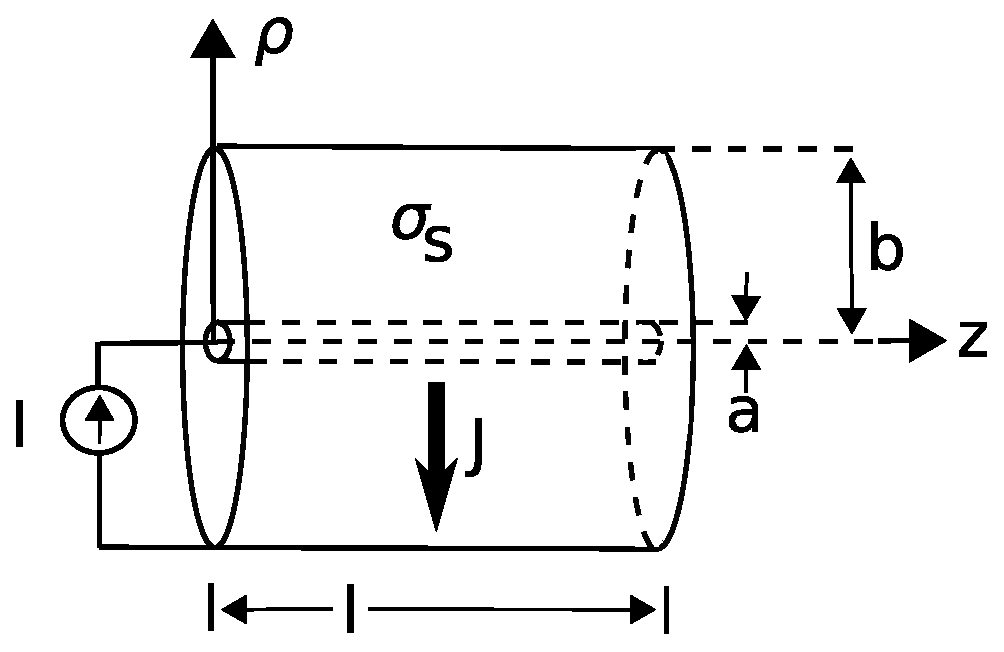
\includegraphics[width=2.5in]{modules/m0105_fCondCoax.eps}
}}{Coaxially-arranged conductor cylinders centered on the z-axis, with the smaller, inner cylinder having radius a, length l, and the larger, outer cylinder having radius b, length l. Current is shown flowing from exterior to interior. A vector, rho, extends from the middle of the inner cylinder upward. A large arrow in the middle of the cylinders points down, labeled bold J. The region between the cylinders has conductance sigma sub s.}
\end{center} 
% URL
%\centerline{\scriptsize 
%\copyright~\hyperref[m0105_fCondCoax_Credit]{Author} 
%\href{https://creativecommons.org/licenses/by-sa/4.0/}{CC BY~SA 4.0} 
%} 
\caption{
\label{m0105_fCondCoax}
Determining the conductance of a structure consisting of coaxially-arranged conductors separated by a lossy dielectric.
}
\end{figure}
\end{example}

%-------------------------------------------------------------------------
 
%ORB EXAMPLE
~\\ \begin{example} 
\begin{mdframed}[backgroundcolor=brown!20,linecolor=brown!20]\raggedright
Conductance of RG-59 
\index{RG-59}
coaxial cable.
\\~\\
RG-59 coaxial cable consists of an inner conductor having radius $0.292$~mm, an outer conductor having radius $1.855$~mm, and a polyethylene spacing material exhibiting conductivity of about $5.9\times 10^{-5}$~S/m.
Estimate the conductance per length of RG-59.

{\bf Solution.} 
From the problem statement, 
$a=0.292$~mm, 
$b=1.855$~mm, 
and $\sigma_s \cong 5.9\times 10^{-5}$~S/m.
Using Equation~\ref{m0105_eGp}, we find $G'\cong 200~\mu$S/m.

\end{mdframed}\end{example}

\index{transmission line!coaxial|)}

\index{conductance|)}

      \vfill\break
    \section{Power Dissipation in Conducting Media}
{\color{blue}\tiny[m0106]}      % This is text associated with the open textbook "Open Electromagnetics"
% See immediately below for author, date
% This work is licensed under the Creative Commons Attribution-ShareAlike 4.0 International License. (CC BY-SA 4.0) 
% To view a copy of the license, visit http://creativecommons.org/licenses/by-sa/4.0/

%ORB TITLE Power Dissipation in Conducting Media
%ORB AUTHOR 0        # S.W. Ellingson, Virginia Tech (ellingson@vt.edu)
%ORB DATE 20180806   # yyyymmdd
%ORB ABSTRACT Power Dissipation in Conducting Media, Joule's Law

\label{m0106_Power_Dissipation_in_Conducting_Media} % <-- Must match name of this file and module directory name.  Don't mess with this!
\index{power dissipation|(}

The displacement of charge in response to the force exerted by an electric field constitutes a reduction in the potential energy of the system (Section~\ref{m0061_Force_Energy_and_Potential_Difference}).
If the charge is part of a steady current, there must be an associated loss of energy that occurs at a steady rate.  
Since power is energy per unit time, the loss of energy associated with current is expressible as power dissipation.
In this section, we address two questions: 
(1) How much power is dissipated in this manner, and
(2) What happens to the lost energy?

First, recall that \emph{work} is force times distance traversed in response to that force (Section~\ref{m0061_Force_Energy_and_Potential_Difference}).  
Stated mathematically:
%
\begin{equation}
\Delta W = +{\bf F}\cdot \Delta {\bf l}
\end{equation}
%
where the vector ${\bf F}$ is the force (units of N) exerted by the electric field, 
the vector $\Delta {\bf l}$ is the direction and distance (units of m) traversed, and
$\Delta W$ is the work done (units of J) as a result. 
Note that a ``$+$'' has been explicitly indicated; this is to emphasize the distinction from the work being considered in Section~\ref{m0061_Force_Energy_and_Potential_Difference}.  In that section, the work ``$\Delta W$'' represented energy from an external source that was being used to increase the potential energy of the system by moving charge ``upstream'' relative to the electric field. 
Now, $\Delta W$ represents this internal energy as it is escaping from the system in the form of kinetic energy; therefore, positive $\Delta W$ now means a reduction in potential energy, hence the sign change.\footnote{It could be argued that it is bad form to use the same variable to represent both tallies; nevertheless, it is common practice and so we simply remind the reader that it is important to be aware of the definitions of variables each time they are (re)introduced.}

The associated power $\Delta P$ (units of W) is $\Delta W$ divided by the time $\Delta t$ (units of s) required for the distance $\Delta{\bf l}$ to be traversed:
%
\begin{equation}
\Delta P = \frac{\Delta W}{\Delta t} = {\bf F}\cdot \frac{\Delta {\bf l}}{\Delta t}
\end{equation}
%
Now we'd like to express force in terms of the electric field exerting this force.
Recall that the force exerted by an electric field intensity ${\bf E}$ (units of V/m) on a particle bearing charge $q$ (units of C) is $q{\bf E}$ (Section~\ref{m0002_Electric_Field_Intensity}).
However, we'd like to express this force in terms of a current, as opposed to a charge.
An expression in terms of current can be constructed as follows. 
First, note that the total charge in a small volume ``cell'' is the volume charge density $\rho_v$ (units of C/m$^3$) times the volume  $\Delta v$ of the cell; i.e., $q = \rho_v \Delta v$ (Section~\ref{m0100_Charge_Distributions}). Therefore: 
%
\begin{equation}
{\bf F} = q{\bf E} = \rho_v~\Delta v~{\bf E}
\end{equation} 
%
and subsequently 
%
\begin{equation}
\Delta P = \rho_v~\Delta v~{\bf E} \cdot \frac{\Delta {\bf l}}{\Delta t} 
         = {\bf E} \cdot \left( \rho_v \frac{\Delta {\bf l}}{\Delta t} \right) \Delta v
\end{equation}
%
The quantity in parentheses has units of C/m$^3$ $\cdot$ m $\cdot$ s$^{-1}$, which is A/m$^2$.
Apparently this quantity is the volume current density ${\bf J}$, so we have  
%
\begin{equation}
\Delta P = {\bf E} \cdot {\bf J}~\Delta v
\end{equation}
%
In the limit as $\Delta v\to 0$ we have
%
\begin{equation}
dP = {\bf E} \cdot {\bf J}~dv
\end{equation}
%
and integrating over the volume ${\mathcal V}$ of interest we obtain
%
\begin{equation}
P = \int_{\mathcal V} dP = \int_{\mathcal V} {\bf E} \cdot {\bf J}~dv
\label{m0106_eJLx}
\end{equation}
%
The above expression is commonly known as \emph{Joule's Law}.
\index{Joule's law}
In our situation, it is convenient to use Ohm's Law 
\index{Ohm's law}
for Electromagnetics (${\bf J}=\sigma{\bf E}$; Section~\ref{m0010_Conductivity}) to get everything in terms of materials properties ($\sigma$), geometry (${\mathcal V}$), and the electric field:
%
\begin{equation}
P = \int_{\mathcal V} {\bf E} \cdot \left(\sigma{\bf E}\right)~dv
\end{equation}
%
which is simply
%
\begin{equation}
\boxed{
P = \int_{\mathcal V} \sigma \left|{\bf E}\right|^2~dv
}
\label{m0106_eJL}
\end{equation}
%
Thus:
%
%ORB HIGHLIGHT
\begin{mdframed}[backgroundcolor=yellow!20,nobreak=true] 
The power dissipation associated with current is given by Equation~\ref{m0106_eJL}. 
This power is proportional to conductivity and proportional to the electric field magnitude squared.
\end{mdframed}

This result facilitates the analysis of power dissipation in materials exhibiting loss; i.e., having finite conductivity.
But what is the power dissipation in a perfectly conducting material?  
For such a material, $\sigma\to\infty$ and ${\bf E}\to 0$ no matter how much current is applied (Section~\ref{m0010_Conductivity}).
In this case, Equation~\ref{m0106_eJL} is not very helpful.
However, as we just noted, being a perfect conductor means ${\bf E}\to 0$ no matter how much current is applied, so from Equation~\ref{m0106_eJLx} we have found that:
%
%ORB HIGHLIGHT
\begin{mdframed}[backgroundcolor=yellow!20,nobreak=true] 
No power is dissipated in a perfect conductor. 
\index{conductor!perfect} 
\end{mdframed}

When conductivity is finite, Equation~\ref{m0106_eJL} serves as a more-general version of a concept from elementary circuit theory, as we shall now demonstrate.
Let ${\bf E}=\hat{\bf z}E_z$, so $\left|{\bf E}\right|^2=E_z^2$.
Then Equation~\ref{m0106_eJL} becomes:
%
\begin{equation}
P = \int_{\mathcal V} \sigma E_z^2~dv = \sigma E_z^2~\int_{\mathcal V}~dv
\label{m0106_ePintegrals}
\end{equation}
%
The second integral in Equation~\ref{m0106_ePintegrals} is a calculation of volume.  
Let's assume ${\mathcal V}$ is a cylinder aligned along the $z$ axis.
The volume of this cylinder is the cross-sectional area $A$ times the length $l$.
Then the above equation becomes:
%
\begin{equation}
P = \sigma E_z^2~A~l 
\end{equation}
%
For reasons that will become apparent very shortly, let's reorganize the above expression as follows:
%
\begin{equation}
P = \left(\sigma E_z A\right) \left(E_z l\right)
\end{equation}
%
Note that $\sigma E_z$ is the current density in A/m$^2$, which when multiplied by $A$ gives the total current.  
Therefore, the quantity in the first set of parentheses is simply the current $I$.
Also note that $E_z l$ is the potential difference over the length $l$, which is simply the node-to-node voltage $V$ (Section~\ref{m0061_Force_Energy_and_Potential_Difference}).
Therefore, we have found:
%
\begin{equation}
P =  IV 
\end{equation}
%
as expected from elementary circuit theory.

Now, what happens to the energy associated with this dissipation of power?
The displacement of charge carriers in the material is limited by the conductivity, which itself is finite because, simply put, other constituents of the material get in the way.  If charge is being displaced as described in this section, then energy is being used to displace the charge-bearing particles.  The motion of constituent particles is observed as heat -- in fact, this is essentially the definition of heat.
Therefore:
%
%ORB HIGHLIGHT
\begin{mdframed}[backgroundcolor=yellow!20,nobreak=true] 
The power dissipation associated with the flow of current in any material that is not a perfect conductor manifests as heat.
\index{heat}
\end{mdframed}
%
This phenomenon is known as \emph{joule heating}, 
\index{joule heating}
\emph{ohmic heating}, 
\index{ohmic heating}
and by other names. 
This conversion of electrical energy to heat is the method of operation for toasters, electric space heaters, and many other devices that generate heat.
It is of course also the reason that all practical electronic devices generate heat.

%%%%%%%%%%%%%%%%%%%%%%%%%%%%%%%%%%%%%%%%%

{\bf Additional Reading:}
\begin{itemize}
\item ``\href{https://en.wikipedia.org/wiki/Joule_heating}{Joule Heating}'' on Wikipedia.
\end{itemize}

\index{power dissipation|)}




%%%      \vfill\break
{\color{blue}\tiny[m0057]}    % This is text associated with the open textbook "Open Electromagnetics"
% See immediately below for author, date
% This work is licensed under the Creative Commons Attribution-ShareAlike 4.0 International License. (CC BY-SA 4.0) 
% To view a copy of the license, visit http://creativecommons.org/licenses/by-sa/4.0/

%ORB TITLE Image Credits
%ORB AUTHOR 0        # S.W. Ellingson, Virginia Tech (ellingson@vt.edu)
%ORB DATE 20180701   # yyyymmdd
%ORB ABSTRACT End matter for chapter entitled "Electrostatics: Steady Current"

\label{m0057_Ch_End_Matter_Electrostatics_Steady_Current} % <-- Must match name of this file and module directory name.  Don't mess with this!

\onecolumn
\section*{Image Credits}

\begin{itemize}

\item[Fig.] \label{m0101_fMatEx1_Credit}
  \ref{m0101_fMatEx1}:
  \copyright~K.\ Kikkeri, 
  \url{https://commons.wikimedia.org/wiki/File:M0101_fMatEx1.svg},\\ 
  CC BY~SA 4.0 (\url{https://creativecommons.org/licenses/by-sa/4.0/}).

\item[Fig.] \label{m0071_fMatEx1_Credit}
  \ref{m0071_fMatEx1}:
  \copyright~K.\ Kikkeri, 
  \url{https://commons.wikimedia.org/wiki/File:M0071_fMatEx1.svg},\\ 
  CC BY~SA 4.0 (\url{https://creativecommons.org/licenses/by-sa/4.0/}).

\end{itemize}

\twocolumn

  \chapter{Magnetostatics}
  \thispagestyle{fancy} % override footer in first page of chapter
  \fancyhf{}            % reset header and footer
  \fancyfoot[C]{\footnotesize \emph{Electromagnetics Vol~1}. ~\copyright~2018 S.W.\ Ellingson ~CC~BY~SA~4.0. ~\url{https://doi.org/10.21061/electromagnetics-vol-1}}
{\color{blue}\tiny[m0117]}    % This is text associated with the open textbook "Open Electromagnetics"
% See immediately below for author, date
% This work is licensed under the Creative Commons Attribution-ShareAlike 4.0 International License. (CC BY-SA 4.0) 
% To view a copy of the license, visit http://creativecommons.org/licenses/by-sa/4.0/

%ORB TITLE Magnetostatics
%ORB AUTHOR 0        # S.W. Ellingson, Virginia Tech (ellingson@vt.edu)
%ORB DATE 20180806   # yyyymmdd
%ORB ABSTRACT Magnetostatics

\label{m0117_Magnetostatics_Preface} % <-- Must match name of this file and module directory name.  Don't mess with this!
\index{magnetostatics (description)}

\emph{Magnetostatics} is the theory of the magnetic field in conditions in which its behavior is independent of electric fields, including
%
\begin{itemize}
\item The magnetic field associated with various spatial distributions of steady current
\item The energy associated with the magnetic field
\item Inductance, which is the ability of a structure to store energy in a magnetic field
\end{itemize}
%
The word ending ``-statics'' refers to the fact that these aspects of electromagnetic theory can be developed by assuming that the sources of the magnetic field are time-invariant; we might say that magnetostatics is the study of the magnetic field at DC.  However, many aspects of magnetostatics are applicable at ``AC'' as well.
 

    \section{Comparison of Electrostatics and Magnetostatics}
{\color{blue}\tiny[m0115]}      % This is text associated with the open textbook "Open Electromagnetics"
% See immediately below for author, date
% This work is licensed under the Creative Commons Attribution-ShareAlike 4.0 International License. (CC BY-SA 4.0) 
% To view a copy of the license, visit http://creativecommons.org/licenses/by-sa/4.0/

%ORB TITLE Comparison of Electrostatics and Magnetostatics 
%ORB AUTHOR 0        # S.W. Ellingson, Virginia Tech (ellingson@vt.edu)
%ORB DATE 20180615   # yyyymmdd
%ORB ABSTRACT Comparison of Electrostatics and Magnetostatics 

\label{m0115_Comparison_of_Electrostatics_and_Magnetostatics} % <-- Must match name of this file and module directory name.  Don't mess with this!

Students encountering magnetostatics 
for the first time have usually been exposed to electrostatics 
already.
Electrostatics and magnetostatics exhibit many similarities.
These are summarized in Table~\ref{m0115_tStaticsDuality}.
The elements of magnetostatics presented in this table are all formally introduced in other sections; the sole purpose of this table is to point out the similarities.  
%
\begin{table*}[t]
\begin{center}
\begin{tabular}{lll}
~ & {\bf electrostatics} & {\bf magnetostatics} \\
\hline\hline
Sources & static charge  & steady current, \\
~ &                      & magnetizable~material \\
\hline
Field intensity & ${\bf E}$ (V/m)  & ${\bf H}$ (A/m) \\
Flux density    & ${\bf D}$ (C/m$^2$) & ${\bf B}$ (Wb/m$^2$=T) \\
\hline
Material relations & ${\bf D}=\epsilon{\bf E}$ & ${\bf B}=\mu{\bf H}$ \\
~                  & ${\bf J}=\sigma{\bf E}$ &  \\
\hline
Force on charge $q$ & ${\bf F}=q{\bf E}$ & ${\bf F}=q{\bf v} \times {\bf B}$ \\
\hline
Maxwell's Eqs. & $\oint_{\mathcal S}{{\bf D}\cdot d{\bf s}} = Q_{encl}$ & $\oint_{\mathcal S}{{\bf B}\cdot d{\bf s}} = 0$ \\
~~(integral)  & $\oint_{\mathcal C}{{\bf E}\cdot d{\bf l}} = 0$ & $\oint_{\mathcal C}{{\bf H}\cdot d{\bf l}} = I_{encl}$ \\
\hline
Maxwell's Eqs. & $\nabla\cdot{\bf D}=\rho_v$ & $\nabla\cdot{\bf B}=0$ \\
~~(differential)   & $\nabla\times{\bf E}=0$ & $\nabla\times{\bf H}={\bf J}$ \\
\hline
Boundary Conditions & $\hat{\bf n} \times \left[{\bf E}_1-{\bf E}_2\right] = 0$     & $\hat{\bf n} \times \left[{\bf H}_1-{\bf H}_2\right] = {\bf J}_s$ \\
~~                  & $\hat{\bf n} \cdot \left[{\bf D}_1-{\bf D}_2\right] = \rho_s$ & $\hat{\bf n} \cdot \left[{\bf B}_1-{\bf B}_2\right] = 0$ \\
\hline
Energy storage & Capacitance & Inductance \\
Energy density & $w_e=\frac{1}{2}\epsilon E^2$ & $w_m=\frac{1}{2}\mu H^2$ \\
Energy dissipation & Resistance &  \\
\hline
\end{tabular}
\end{center}
\label{m0115_tStaticsDuality}
\caption{A summary of the duality between electrostatics and magnetostatics.}
\end{table*}

The technical term for these similarities is \emph{duality}.
\index{duality}
Duality also exists between voltage and current in electrical circuit theory.
For more about the concept of duality, see ``Additional Reading'' at the end of this section.

%%%%%%%%%%%%%%%%%%%%%%%%%%%%%%%%%%%%%%%%%

{\bf Additional Reading:}
\begin{itemize}
\item ``\href{https://en.wikipedia.org/wiki/Duality_(electricity_and_magnetism)}{Duality (electricity and magnetism)}'' on Wikipedia.
\item ``\href{https://en.wikipedia.org/wiki/Duality_(electrical_circuits)}{Duality (electrical circuits)}'' on Wikipedia.
\end{itemize}






      \vfill\break
    \section{Gauss' Law for Magnetic Fields: Integral Form}
{\color{blue}\tiny[m0018]}      % This is text associated with the open textbook "Open Electromagnetics"
% See immediately below for author, date
% This work is licensed under the Creative Commons Attribution-ShareAlike 4.0 International License. (CC BY-SA 4.0) 
% To view a copy of the license, visit http://creativecommons.org/licenses/by-sa/4.0/

%ORB TITLE Gauss' Law for Magnetic Fields: Integral Form 
%ORB AUTHOR 0        # S.W. Ellingson, Virginia Tech (ellingson@vt.edu)
%ORB DATE 20180628   # yyyymmdd
%ORB ABSTRACT Gauss' Law for Magnetic Fields: Integral Form  

\label{m0018_Gauss_Law_Magnetic_Integral_Form} % <-- Must match name of this file and module directory name.  Don't mess with this!
\index{Gauss' law!magnetic field|(}

Gauss' Law for Magnetic Fields (GLM) is one of the four fundamental laws of classical electromagnetics, collectively known as \emph{Maxwell's Equations}.
Before diving in, the reader is strongly encouraged to review Section~\ref{m0003_Magnetic_Flux_Density}.
In that section, GLM emerges from the ``flux density'' interpretation of the magnetic field.  GLM is not identified in that section, but now we are ready for an explicit statement:
%
%ORB HIGHLIGHT
\begin{mdframed}[backgroundcolor=yellow!20,nobreak=true] 
\emph{Gauss' Law for Magnetic Fields} (Equation~\ref{m0018_eGLM}) states that the flux of the magnetic field through a closed surface is zero.
\end{mdframed}
%
This is expressed mathematically as follows:
%
\begin{equation}
\boxed{
\oint_{\mathcal S} {\bf B}\cdot d{\bf s} = 0
}
\label{m0018_eGLM}
\end{equation}
%
where 
${\bf B}$ is magnetic flux density and
${\mathcal S}$ is a closed surface with outward-pointing differential surface normal $d{\bf s}$.
It may be useful to consider the units.
${\bf B}$ has units of Wb/m$^{2}$; therefore, integrating ${\bf B}$ over a surface gives a quantity with units of Wb, which is magnetic flux, as indicated above.

GLM can also be interpreted in terms of magnetic field lines.  For the magnetic flux through a closed surface to be zero, every field line entering the volume enclosed by ${\mathcal S}$ must also exit this volume -- field lines may not begin or end within the volume.
The only way this can be true for every possible surface ${\mathcal S}$ is if magnetic field lines always form closed loops. 
This is in fact what we find in practice, as shown in Figure~\ref{m0018_fGLMBarMagnet}.
%
\begin{figure}
\begin{center}
\pdftooltip{{  % note double braces
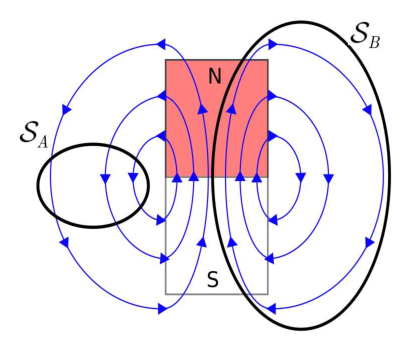
\includegraphics[width=\columnwidth]{modules/m0018_fGLMBarMagnet.eps}
% https://commons.wikimedia.org/wiki/File:M0018_fGLMBarMagnet_(2).svg
}}{A bar magnet oriented vertically with the north pole at the top. The magnetic field is shown by two sets of concentric curves labeled "B" that mirror each other on the left and right sides of the magnet. They are centered on the horizontal axis where the north and south poles meet. The left-side curves have arrows that indicate counterclockwise direction. The right-side curves have a clockwise direction. A large, bold oval lays over the middle of the curves on the left, labeled S sub A. A larger, bold oval lays over all of the curves on the right, labeled S sub B.}
\end{center} 
\centerline{\scriptsize 
\copyright~\hyperref[m0018_fGLMBarMagnet_Credit]{Youming / K.\ Kikkeri} 
\href{https://creativecommons.org/licenses/by-sa/4.0/}{CC BY~SA 4.0} 
} 
\caption{
\label{m0018_fGLMBarMagnet}
Gauss' Law for Magnetostatics applied to a two-dimensional bar magnet.  
For the surface ${\mathcal S}={\mathcal S}_A$, every field line entering ${\mathcal S}$ also leaves ${\mathcal S}$, so the flux through ${\mathcal S}$ is zero.
For the surface ${\mathcal S}={\mathcal S}_B$, every field line within ${\mathcal S}$ remains in ${\mathcal S}$, so the flux through ${\mathcal S}$ is again zero.
}
\end{figure}

Following this argument one step further, GLM implies there can be no particular particle or structure that can be the source of the magnetic field (because then that would be a start point for field lines).
This is one way in which the magnetic field is very different from the electrostatic field, for which every field line begins at a charged particle.
So, when we say that current (for example) is the source of the magnetic field, we mean only that the field coexists with current, and \emph{not} that the magnetic field is somehow attached to the current.
Summarizing, there is no ``localizable'' quantity, analogous to charge for electric fields, associated with magnetic fields.  This is just another way in which magnetic fields are weird! 

Summarizing:
%
%ORB HIGHLIGHT
\begin{mdframed}[backgroundcolor=yellow!20,nobreak=true] 
Gauss' Law for Magnetic Fields requires that magnetic field lines form closed loops.  Furthermore, there is no particle that can be identified as the source of the magnetic field.  
\end{mdframed}


{\bf Additional Reading:}
\begin{itemize}
\item ``\href{https://en.wikipedia.org/wiki/Gauss'_law_for_magnetism}{Gauss' Law for Magnetism}'' on Wikipedia.
\item ``\href{https://en.wikipedia.org/wiki/Maxwell's_equations}{Maxwell's Equations}'' on Wikipedia.
\end{itemize}

\index{Gauss' law!magnetic field|)}

      \vfill\break
    \section{Gauss' Law for Magnetism: Differential Form}
{\color{blue}\tiny[m0047]}      
% This is text associated with the open textbook "Open Electromagnetics"
% See immediately below for author, date
% This work is licensed under the Creative Commons Attribution-ShareAlike 4.0 International License. (CC BY SA 4.0) 
% To view a copy of the license, visit http://creativecommons.org/licenses/by-sa/4.0/

%ORB TITLE Gauss' Law for Magnetism: Differential Form 
%ORB AUTHOR 0        # S.W. Ellingson, Virginia Tech (ellingson@vt.edu)
%ORB DATE 20180806   # yyyymmdd
%ORB ABSTRACT Gauss' Law for Magnetism: Differential Form from Integral Form

\label{m0047_Gauss_Law_Magnetic_Differential_from_Integral} % <-- Must match name of this file and module directory name.  Don't mess with this!

The integral form of Gauss' Law (Section~\ref{m0018_Gauss_Law_Magnetic_Integral_Form}) states that the magnetic flux through a closed surface is zero.
In mathematical form:
%
\begin{equation}
\oint_{\mathcal S} {\bf B}\cdot d{\bf s} = 0
\label{m0047_eGLMIF}
\end{equation}
%
where ${\bf B}$ is magnetic flux density and ${\mathcal S}$ is the enclosing surface.
Just as Gauss's Law for electrostatics has both integral (Sections~\ref{m0014_Gauss_Law_Integral_Form}) and differential (Section~\ref{m0045_Gauss_Law_Differential_Form_from_Integral_Form}) forms, so too does Gauss' Law for Magnetic Fields.
Here we are interested in the differential form for the same reason.  Given a differential equation and the boundary conditions imposed by structure and materials, we may then solve for the magnetic field in very complicated scenarios.  

The equation we seek may be obtained from Equation~\ref{m0047_eGLMIF} using the Divergence Theorem 
\index{divergence theorem}
(Section~\ref{m0046_Divergence_Theorem}), which in the present case may be written:
%
\begin{equation}
\int_{\mathcal V} \left( \nabla \cdot {\bf B} \right) dv = \oint_{\mathcal S} {\bf B}\cdot d{\bf s}
\end{equation}
%
Where ${\mathcal V}$ is the mathematical volume bounded by the closed surface ${\mathcal S}$.
From Equation~\ref{m0047_eGLMIF} we see that the right hand side of the equation is zero, leaving:
%
\begin{equation}
\int_{\mathcal V} \left( \nabla \cdot {\bf B} \right) dv = 0
\end{equation}
%
The above relationship must hold regardless of the specific location or shape of ${\mathcal V}$.  The only way this is possible is if the integrand is everywhere equal to zero.  We conclude:
%
\begin{equation}
\boxed{
\nabla \cdot {\bf B}=0
}
\label{m0047_eGLMD}
\end{equation}
%
%ORB HIGHLIGHT
\begin{mdframed}[backgroundcolor=yellow!20,nobreak=true] 
The differential (``point'') form of Gauss' Law for Magnetic Fields (Equation~\ref{m0047_eGLMD}) states that the flux per unit volume of the magnetic field is always zero.
\end{mdframed}
%
This is another way of saying that there is no point in space that can be considered to be the source of the magnetic field, for if it were, then the total flux through a bounding surface would be greater than zero. 
Said yet another way, the source of the magnetic field is not localizable.



%-------------------------------------------------------

{\bf Additional Reading:}
\begin{itemize}
\item ``\href{https://en.wikipedia.org/wiki/Gauss'_law_for_magnetism}{Gauss' Law for Magnetism}'' on Wikipedia.
\end{itemize}




      \vfill\break
    \section{Ampere's Circuital Law (Magnetostatics): Integral Form}
{\color{blue}\tiny[m0019]}      % This is text associated with the open textbook "Open Electromagnetics"
% See immediately below for author, date
% This work is licensed under the Creative Commons Attribution-ShareAlike 4.0 International License. (CC BY-SA 4.0) 
% To view a copy of the license, visit http://creativecommons.org/licenses/by-sa/4.0/

%ORB TITLE Ampere's Circuital Law (Magnetostatics): Integral Form
%ORB AUTHOR 0        # S.W. Ellingson, Virginia Tech (ellingson@vt.edu)
%ORB DATE 20180806   # yyyymmdd
%ORB ABSTRACT Ampere's Circuital Law (Magnetostatics): Integral Form

\label{m0019_Amperes_Law_Magnetostatics} % <-- Must match name of this file and module directory name.  Don't mess with this!
\index{Ampere's law!magnetostatics|(}

Ampere's circuital law (ACL) relates current to the magnetic field associated with the current.
In the magnetostatic regime, the law is (see also Figure~\ref{m0019_fACL}):
%
\begin{equation}   
\boxed{
\oint_{\mathcal C}{ {\bf H} \cdot d{\bf l} } = I_{encl}  
}
\label{m0019_eACL}
\end{equation}
%
That is, the integral of the magnetic field intensity ${\bf H}$ over a closed path ${\mathcal C}$ is equal to the current enclosed by that path, $I_{encl}$.
Before proceeding to interpret this law, it is useful to see that it is dimensionally correct. 
That is, ${\bf H}$ (units of A/m) integrated over a distance (units of m) yields a quantity with units of current (i.e., A).
%
\begin{figure}[b!]
\begin{center}
\pdftooltip{{  % note double braces
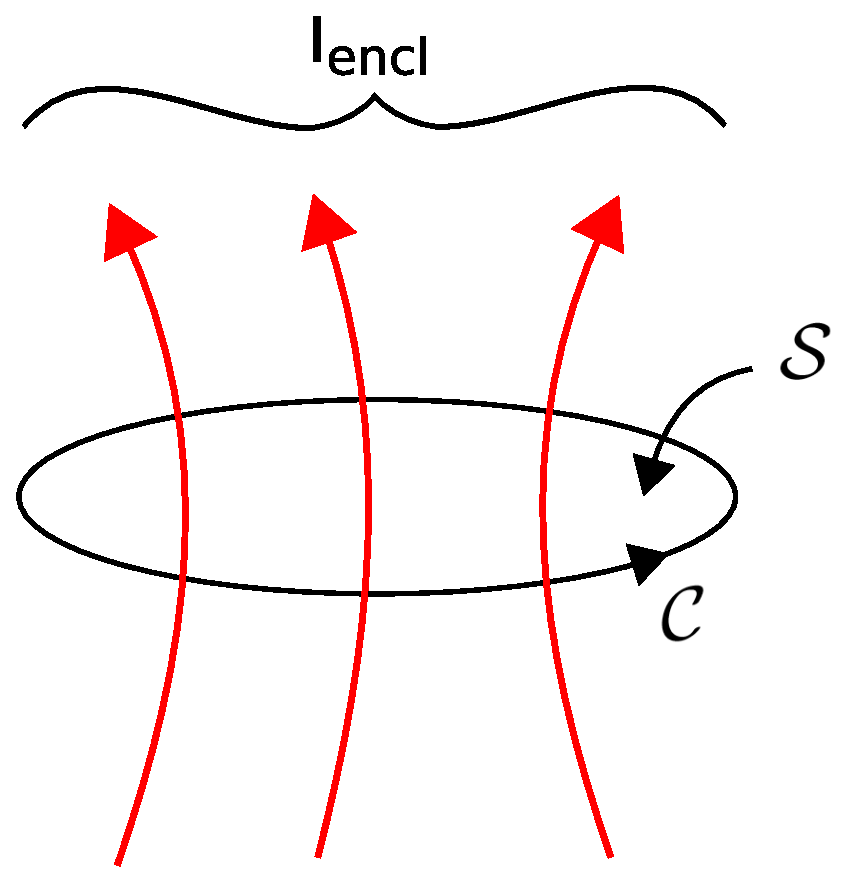
\includegraphics[width=1.5in]{modules/m0019_fACL.eps}
% https://commons.wikimedia.org/wiki/File:M0019_fACL.svg
}}{The figure shows a circle, with surface S and path C. On the path, C, is an arrow that points to the right to indicate counter-clockwise direction. Through the circle are three vectors, the left two bent slightly to the left and the right one bent slightly to the right. All three vectors are labeled "I sub encl".}
\end{center} 
\centerline{\scriptsize 
\copyright~\hyperref[m0019_fACL_Credit]{K.\ Kikkeri} 
\href{https://creativecommons.org/licenses/by-sa/4.0/}{CC BY~SA 4.0} 
} 
\caption{
\label{m0019_fACL}
Reference directions for Ampere's Circuital Law (Equation~\ref{m0019_eACL}).
}
\end{figure}    

In general, $I_{encl}$ may be either positive or negative.
The direction corresponding to positive current flow must be correctly associated with ${\mathcal C}$.
The relationship follows the \emph{right-hand rule} of Stokes' Theorem (Section~\ref{m0051_Stokes_Theorem}) summarized as follows.  The direction of positive $I_{encl}$ is the direction in which the fingers of the right hand intersect any surface ${\mathcal S}$ bordered by ${\mathcal C}$ when the thumb of the right hand points in the direction of integration. The connection to Stokes' Theorem is not a coincidence. See Section~\ref{m0118_Amperes_Law_Magnetostatics_Integral-to-Differential} for more about this.

Note that ${\mathcal S}$ can be \emph{any} surface that is bounded by ${\mathcal C}$ -- not just the taut surface implied in Figure~\ref{m0019_fACL}.

%ORB HIGHLIGHT
\begin{mdframed}[backgroundcolor=yellow!20,nobreak=true] 
The integral form of Ampere's Circuital Law for magnetostatics (Equation~\ref{m0019_eACL}) relates the magnetic field along a closed path to the total current flowing through any surface bounded by that path.
\end{mdframed}

ACL plays a role in magnetostatics that is very similar to the role played by the integral form of Gauss' Law in electrostatics (Section~\ref{m0014_Gauss_Law_Integral_Form}). 
That is, ACL provides a means calculate the magnetic field given the source current.
ACL also has a similar limitation.  Generally, symmetry is required to simplify the problem sufficiently so that the integral equation may be solved.
Fortunately, a number of important problems fall in this category.
Examples include the problems addressed in
Sections~\ref{m0119_Magnetic_Field_of_a_Long_Wire} (magnetic field of a line current), 
\ref{m0120_Magnetic_Field_of_a_Coil} (magnetic field inside a straight coil), 
\ref{m0049_Magnetic_Field_of_a_Toroidal_Coil} (magnetic field of a toroidal coil), 
\ref{m0121_Magnetic_Field_of_an_Infinite_Current_Sheet} (magnetic field of a current sheet), and 
\ref{m0023_Boundary_Conditions_on_H} (boundary conditions on the magnetic field intensity).
For problems in which the necessary symmetry is not available, the differential form of ACL may be required (Section~\ref{m0118_Amperes_Law_Magnetostatics_Integral-to-Differential}).

Finally, be aware that the form of ACL addressed here applies to magnetostatics only.  
In the presence of a \emph{time-varying} electric field, the right side of ACL includes an additional term known as the \emph{displacement current}
\index{displacement current} 
\index{current!displacement|see{displacement current}}
(Section~\ref{m0053_Displacement_Current_Amperes_Law}).

%-------------------------------------------------------

{\bf Additional Reading:}
\begin{itemize}
\item ``\href{https://en.wikipedia.org/wiki/Maxwell's_equations}{Maxwell's Equations}'' on Wikipedia.
\item ``\href{https://en.wikipedia.org/wiki/Ampere's_circuital_law}{Ampere's Circuital Law}'' on Wikipedia.
\end{itemize}

\index{Ampere's law!magnetostatics|)}

      \vfill\break
    \section{Magnetic Field of an Infinitely-Long Straight Current-Bearing Wire}
{\color{blue}\tiny[m0119]}      % This is text associated with the open textbook "Open Electromagnetics"
% See immediately below for author, date
% This work is licensed under the Creative Commons Attribution-ShareAlike 4.0 International License. (CC BY SA 4.0) 
% To view a copy of the license, visit http://creativecommons.org/licenses/by-sa/4.0/

%ORB TITLE Magnetic Field of an Infinitely-Long Straight Current-Bearing Wire
%ORB AUTHOR 0        # S.W. Ellingson, Virginia Tech (ellingson@vt.edu)
%ORB DATE 20180806   # yyyymmdd
%ORB ABSTRACT Magnetic Field of an Infinitely-Long Straight Line Current

\label{m0119_Magnetic_Field_of_a_Long_Wire} % <-- Must match name of this file and module directory name.  Don't mess with this!

In this section, we use the magnetostatic form of Ampere's Circuital Law 
\index{Ampere's law!magnetostatics}
(ACL) (Section~\ref{m0019_Amperes_Law_Magnetostatics}) to determine the magnetic field due to a steady current $I$ (units of A) in an infinitely-long straight wire.
The problem is illustrated in Figure~\ref{m0119_fLSW}.
The wire is an electrically-conducting circular cylinder of radius $a$.
Since the wire is a cylinder, the problem is easiest to work in cylindrical coordinates with the wire aligned along the $z$ axis.
%
\begin{figure}[b!]
\begin{center}
\pdftooltip{{  % note double braces
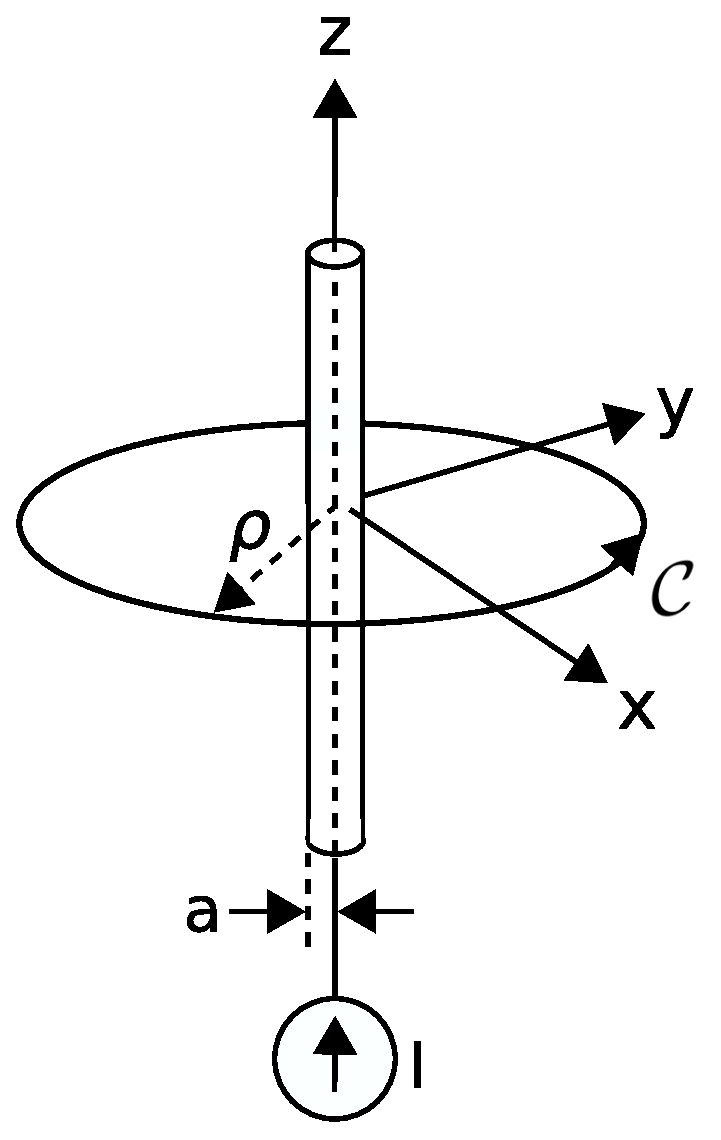
\includegraphics[width=2in]{modules/m0119_fLSW.eps}
% https://commons.wikimedia.org/wiki/File:M0119_fLSW.svg
}}{A small cylinder with radius a represents a wire, centered vertically on the z-axis in a Cartesian coordinate system. From the bottom, current is pointed upward through the wire. Around the middle of the wire is a circular path C, with an arrow on the path pointed counterclockwise to indicate direction. A dashed vector, rho, extends out of the middle of the wire to the left to the path, perpendicular to the z-axis.}
\end{center} 
\centerline{\scriptsize 
\copyright~\hyperref[m0119_fLSW_Credit]{K.\ Kikkeri} 
\href{https://creativecommons.org/licenses/by-sa/4.0/}{CC BY~SA 4.0} 
} 
\caption{
\label{m0119_fLSW}
Determination of the magnetic field due to steady current in an infinitely-long straight wire.
}
\end{figure}  

Here's the relevant form of ACL:
%
\begin{equation}   
\oint_{\mathcal C}{ {\bf H} \cdot d{\bf l} } = I_{encl}  
\label{m0119_eACL}
\end{equation}
%
where $I_{encl}$ is the current enclosed by the closed path ${\mathcal C}$.
ACL works for {\it any} closed path, so to exploit the symmetry of the cylindrical coordinate system we choose a circular path of radius $\rho$ in the $z=0$ plane, centered at the origin.  
With this choice we have 
%
\begin{equation}
I_{encl}=I ~~ \mbox{for}~\rho\ge a
\end{equation}

For $\rho<a$, we see that $I_{encl}<I$.  
a steady (DC) current will be distributed uniformly throughout the wire (Section~\ref{m0071_Resistance_DC}).
Since the current is uniformly distributed over the cross section, $I_{encl}$ is less than the total current $I$ by the same factor that the area enclosed by ${\mathcal C}$ is less than $\pi a^2$, the cross-sectional area of the wire.
The area enclosed by ${\mathcal C}$ is simply $\pi \rho^2$, so we have
%
\begin{equation}
I_{encl}
=I \frac{\pi \rho^2}{\pi a^2}
=I \frac{\rho^2}{a^2} ~~ \mbox{for}~\rho<a
\end{equation}
 
For the choice of ${\mathcal C}$ made above, Equation~\ref{m0119_eACL} becomes
%
\begin{equation}   
\int_{\phi=0}^{2\pi} { {\bf H} \cdot \left(\hat{\bf \phi}~\rho~d\phi\right) } = I_{encl}
\label{m0119_eACL1}
\end{equation}
%
Note that we have chosen to integrate in the $+\phi$ direction.
Therefore, the right-hand rule 
\index{right-hand rule!Stokes' theorem}
specifies that positive $I_{encl}$ corresponds to current flowing in the $+z$ direction, which is consistent with the direction indicated in Figure~\ref{m0119_fLSW}.
(Here's an excellent exercise to test your understanding. Change the direction of the path of integration and confirm that you get the same result obtained at the end of this section.  Changing the direction of integration should not change the magnetic field associated with the current!)

The simplest way to solve for ${\bf H}$ from Equation~\ref{m0119_eACL1} is to use a symmetry 
\index{symmetry}
argument, which proceeds as follows: 
%
\begin{itemize}
\item Since the distribution of current is uniform and infinite in the $z$-dimension, ${\bf H}$ can't depend on $z$, and so ${\bf H}\cdot\hat{\bf z}$ must be zero everywhere.
\item The problem is identical after any amount of rotation in $\phi$; therefore, the magnitude of ${\bf H}$ cannot depend on $\phi$. 
This is a form of radial symmetry.  
Since we determined above that ${\bf H}$ can't depend on $z$ either, it must be that the magnitude of ${\bf H}$ can depend only on $\rho$.  
\item The radial symmetry of the problem also requires that ${\bf H}\cdot\hat{\bf \rho}$ be equal to zero.  If this were not the case, then the field would not be radially symmetric.  Since we determined above that ${\bf H}\cdot\hat{\bf z}$ is also zero, ${\bf H}$ must be entirely $\pm\hat{\bf \phi}$-directed.
\end{itemize}
%
From the above considerations, the most general form of the magnetic field intensity can be written ${\bf H} = \hat{\bf \phi}H(\rho)$.  Substituting this into Equation~\ref{m0119_eACL1}, we obtain
%
\begin{flalign}   
I_{encl} &= \int_{\phi=0}^{2\pi} { \left[\hat{\bf \phi}H(\rho)\right] \cdot \left(\hat{\bf \phi}~\rho~d\phi\right) } \nonumber \\
         &= \rho H(\rho)~\int_{\phi=0}^{2\pi} { d\phi } \nonumber \\
         &= 2\pi \rho H(\rho)
\end{flalign}
%
Therefore, $H(\rho)=I_{encl}/2\pi \rho$.  Reassociating the known direction, we obtain:
%
\begin{equation}  
{\bf H}  = \hat{\bf \phi}\frac{I_{encl}}{2\pi \rho}
\end{equation}
%
Therefore, the field outside of the wire is:
%
\begin{equation} 
\boxed{  
{\bf H}  = \hat{\bf \phi}\frac{I}{2\pi \rho} ~~ \mbox{for} ~ \rho\ge a
}
\label{m0119_eACLLCe}
\end{equation}
%
whereas the field inside the wire is:
%
\begin{equation} 
\boxed{  
{\bf H}  = \hat{\bf \phi}\frac{I\rho}{2\pi a^2} ~~ \mbox{for} ~ \rho<a
}
\label{m0119_eACLLCi}
\end{equation}
%
(By the way, this is a good time for a units check.)

Note that as $\rho$ increases from zero to $a$ (i.e., inside the wire), the magnetic field is proportional to $\rho$ and therefore increases.
However, as $\rho$ continues to increase beyond $a$ (i.e., outside the wire), the magnetic field is proportional to $\rho^{-1}$ and therefore decreases.

If desired, the associated magnetic flux density can be obtained using ${\bf B} = \mu {\bf H}$.

Summarizing:
%
%ORB HIGHLIGHT
\begin{mdframed}[backgroundcolor=yellow!20,nobreak=true] 
The magnetic field due to current in an infinite straight wire is given by Equations~\ref{m0119_eACLLCe} (outside the wire) and \ref{m0119_eACLLCi} (inside the wire).
The magnetic field is $+\hat{\bf \phi}$-directed for current flowing in the $+z$ direction,
so the magnetic field lines form concentric circles perpendicular to and centered on the wire.
\end{mdframed}

Finally, we point out another ``right-hand rule'' 
\index{right-hand rule!magnetic field of a wire}
that emerges from this solution, shown in Figure~\ref{m0119_fRightHandRule} and summarized below:
%
%ORB HIGHLIGHT
\begin{mdframed}[backgroundcolor=yellow!20,nobreak=true] 
The magnetic field due to current in an infinite straight wire points in the direction of the curled fingers of the right hand when the thumb of the right hand is aligned in the direction of current flow. 
\end{mdframed}
%
This simple rule turns out to be handy in quickly determining the relationship between the directions of the magnetic field and current flow in many other problems, and so is well worth committing to memory.
%
\begin{figure}
\begin{center}
\pdftooltip{{  % note double braces
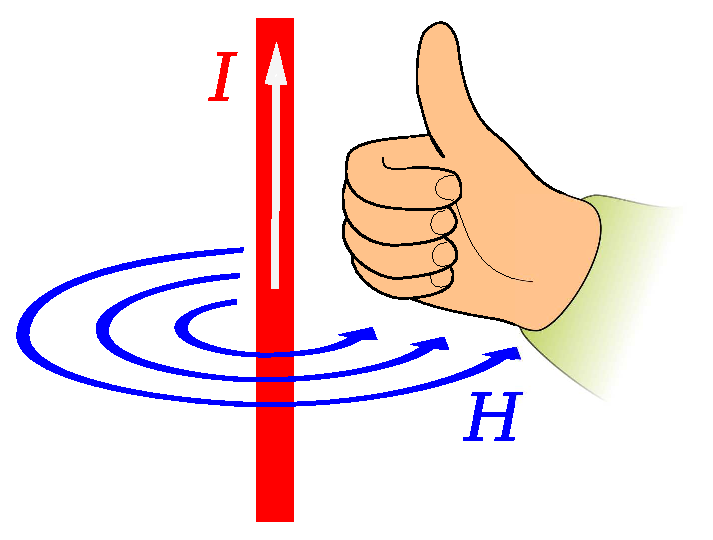
\includegraphics[width=2in]{modules/m0119_fRightHandRule.eps}
% https://et.wikipedia.org/wiki/Fail:Manoderecha.svg
}}{A red wire lies vertically, with a vector in the middle pointing up to represent current. Three blue, concentric circles lie around the middle of the rectangle, labeled H. To the right of the rectangle is a right hand, with the thumb pointed up and fingers curled. }
\end{center} 
\centerline{\scriptsize 
\copyright~\hyperref[m0119_fRightHandRule_Credit]{Jfmelero} 
\href{https://creativecommons.org/licenses/by-sa/4.0/}{CC BY~SA 4.0} (modified)
} 
\caption{
\label{m0119_fRightHandRule}
Right-hand rule for the relationship between the direction of current and the direction of the magnetic field.
}
\end{figure}  






      \vfill\break
    \section{Magnetic Field Inside a Straight Coil}
{\color{blue}\tiny[m0120]}      % This is text associated with the open textbook "Open Electromagnetics"
% See immediately below for author, date
% This work is licensed under the Creative Commons Attribution-ShareAlike 4.0 International License. (CC BY SA 4.0) 
% To view a copy of the license, visit http://creativecommons.org/licenses/by-sa/4.0/

%ORB TITLE Magnetic Field Inside a Straight Coil
%ORB AUTHOR 0        # S.W. Ellingson, Virginia Tech (ellingson@vt.edu)
%ORB DATE 20180628   # yyyymmdd
%ORB ABSTRACT Magnetic Field Inside a Coil

\label{m0120_Magnetic_Field_of_a_Coil} % <-- Must match name of this file and module directory name.  Don't mess with this!
\index{coil|(}

In this section, we use the magnetostatic integral form of Ampere's Circuital Law 
\index{Ampere's law!magnetostatics}
(ACL) (Section~\ref{m0019_Amperes_Law_Magnetostatics}) to determine the magnetic field inside a straight coil of the type shown in Figure~\ref{m0120_fStraightCoil} in response to a steady (i.e., DC) current.
The result has a number of applications, including the analysis and design of inductors, 
\index{inductor}
solenoids 
\index{solenoid}
(coils that are used as magnets, typically as part of an actuator), and as a building block and source of insight for more complex problems.
%
\begin{figure}[b!]
\begin{center}
\pdftooltip{{  % note double braces
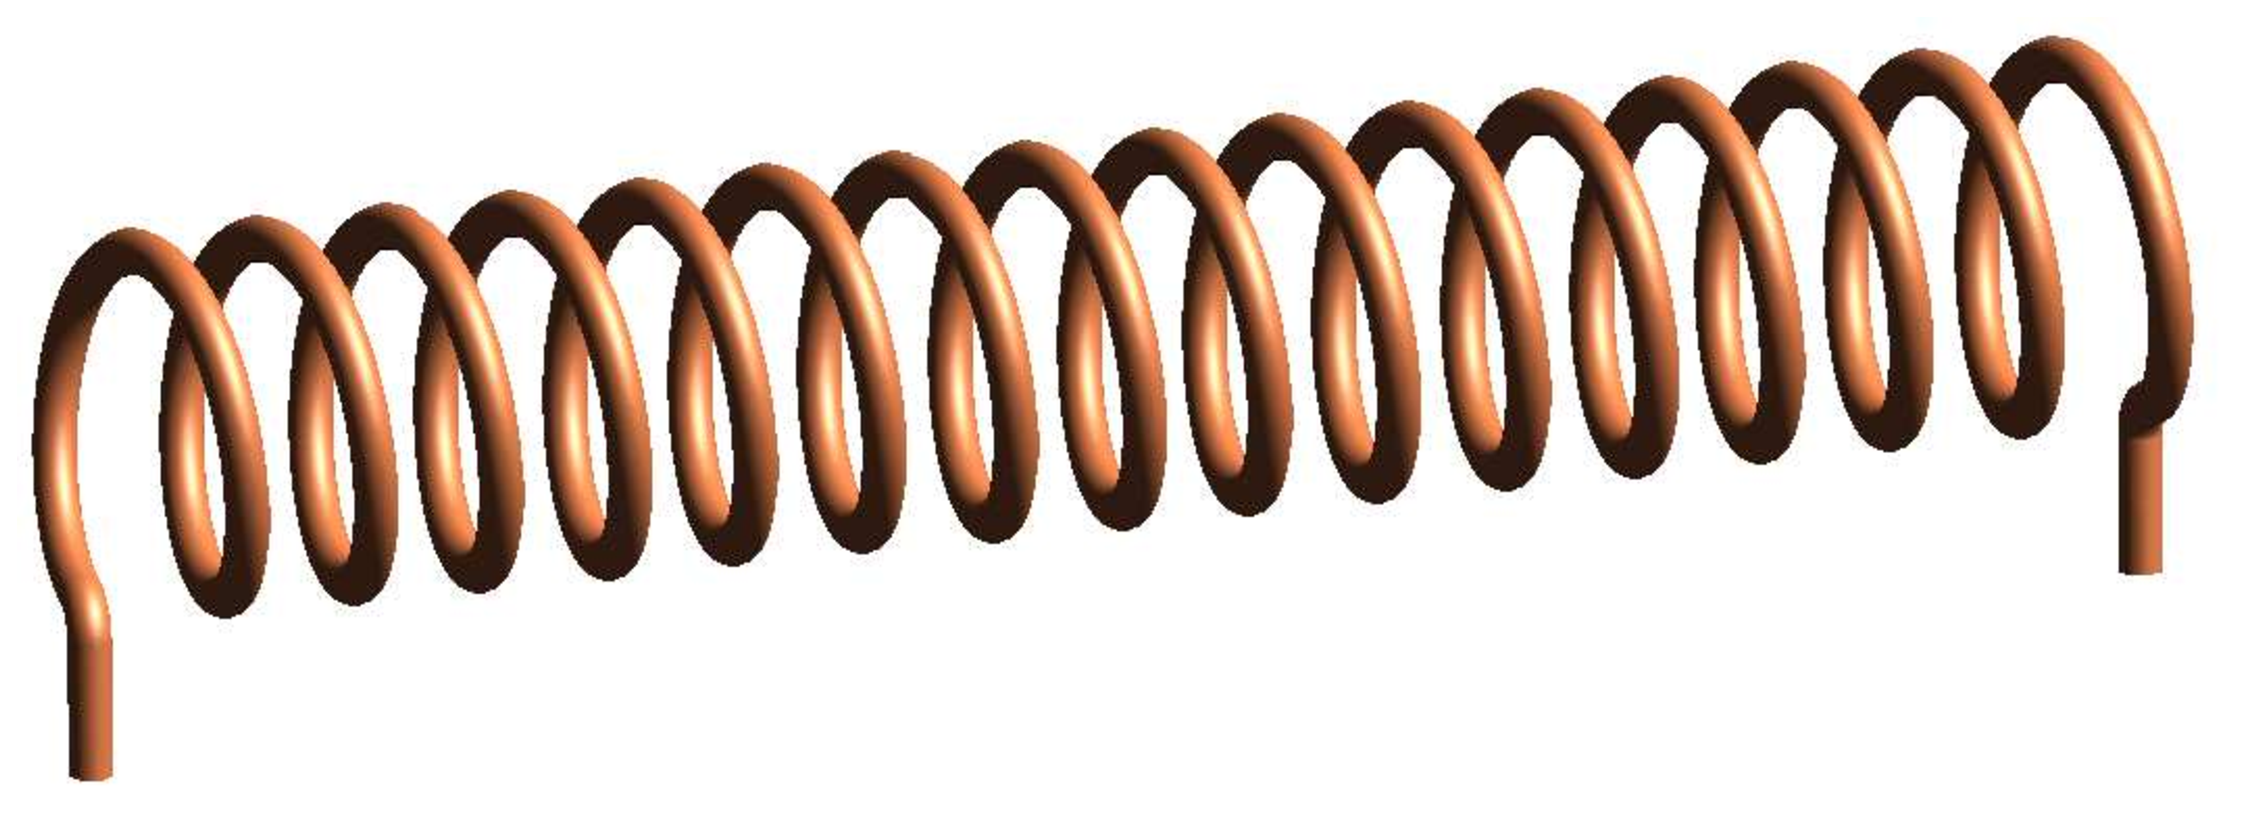
\includegraphics[width=1.5in]{modules/m0120_fStraightCoil.eps}
% https://en.wikipedia.org/wiki/File:Solenoid-1.png
}}{A circular coil, with uniform turns.}
\end{center} 
\centerline{\scriptsize 
by~\hyperref[m0120_fStraightCoil_Credit]{Zureks} (public domain)
%\href{https://creativecommons.org/licenses/by-sa/4.0/}{CC BY~SA 4.0} 
} 
\caption{
\label{m0120_fStraightCoil}
A straight coil.
}
\end{figure}  

The present problem is illustrated in Figure~\ref{m0120_fCoil}.
The coil is circular with radius $a$ and length $l$, and consists of $N$ turns (``windings'') of wire wound with uniform winding density.
Since the coil forms a cylinder, the problem is easiest to work in cylindrical coordinates with the axis of the coil aligned along the $z$ axis.
%
\begin{figure}
\begin{center}
\pdftooltip{{  % note double braces
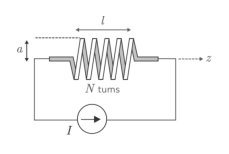
\includegraphics[width=2.5in]{modules/m0120_fCoil.eps}
}}{A circular coil with radius a and length l, consisting of N turns wound uniformly lies on the z-axis in a series circuit with current pointed to the right running counterclockwise.}
\end{center} 
% ***WikipediaCommonsURL
%\centerline{\scriptsize 
%\copyright~\hyperref[m0120_fCoil_Credit]{author} 
%\href{https://creativecommons.org/licenses/by-sa/4.0/}{CC BY-SA 4.0} 
%} 
\caption{
\label{m0120_fCoil}
Determination of the magnetic field due to DC current in a coil.
}
\end{figure}  

To begin, let's take stock of what we already know about the answer, which is actually quite a bit.
The magnetic field deep inside the coil is generally aligned with axis of the coil as shown in Figure~\ref{m0120_fStraightCoilFieldLines}.
This can be explained using the result for the magnetic field due to a straight line current (Section~\ref{m0119_Magnetic_Field_of_a_Long_Wire}), in which we found that the magnetic field follows a ``right-hand rule.'' 
\index{right-hand rule!magnetic field of a wire}
The magnetic field points in the direction of the fingers of the right hand when the thumb of the right hand is aligned in the direction of current flow. 
The wire comprising the coil is obviously \emph{not} straight, but we can consider just one short segment of one turn and then sum the results for all such segments.
When we consider this for a single turn of the coil, the situation is as shown in Figure~\ref{m0120_fOneTurn}.
Summing the results for many loops, we see that the direction of the magnetic field inside the coil must be generally in the $+\hat{\bf z}$ direction when the current $I$ is applied as shown in Figures~\ref{m0120_fCoil} and \ref{m0120_fStraightCoilFieldLines}.
However, there is one caveat. The windings must be sufficiently closely-spaced that the magnetic field lines can only pass through the openings at the end of the coil and  do not take any ``shortcuts'' between individual windings.
%
\begin{figure}
\begin{center}
\pdftooltip{{  % note double braces
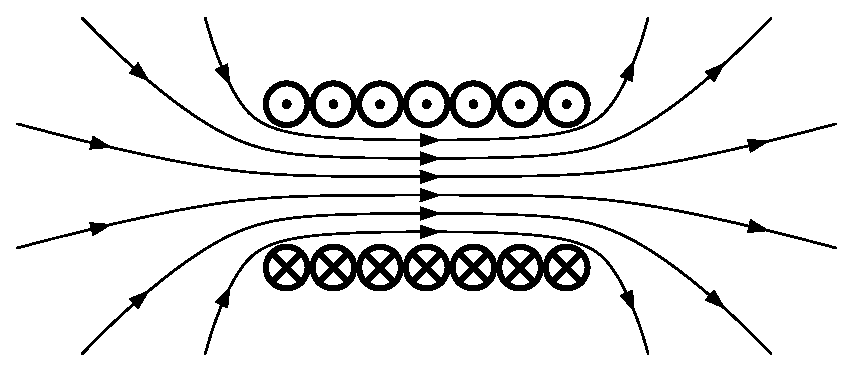
\includegraphics[width=2.5in]{modules/m0120_fStraightCoilFieldLines.eps}
% https://commons.wikimedia.org/wiki/File:VFPt_Solenoid_correct.svg
}}{Two rows of circles lie horizontally, parallel from each other. The circles on the top row all have dots in the middle. The circles on the bottom row all have x’s in the middle. Going through the space between the two rows are magnetic field lines. They fan inward from the left, become parallel when they are between the rows, and fan out on the right. Arrows on all of the field lines point to the right to indicate direction.}
\end{center} 
\centerline{\scriptsize 
\copyright~\hyperref[m0120_fStraightCoilFieldLines_Credit]{Geek3} 
\href{https://creativecommons.org/licenses/by-sa/3.0/}{CC BY~SA 3.0} 
} 
\caption{
\label{m0120_fStraightCoilFieldLines}
Magnetic field lines inside a straight coil with closely-spaced windings. (Dotted circles represent current flowing up/out from the page; crossed circles represent current flowing down/into the page.)
}
\end{figure}  
%
\begin{figure}
\begin{center}
\pdftooltip{{  % note double braces
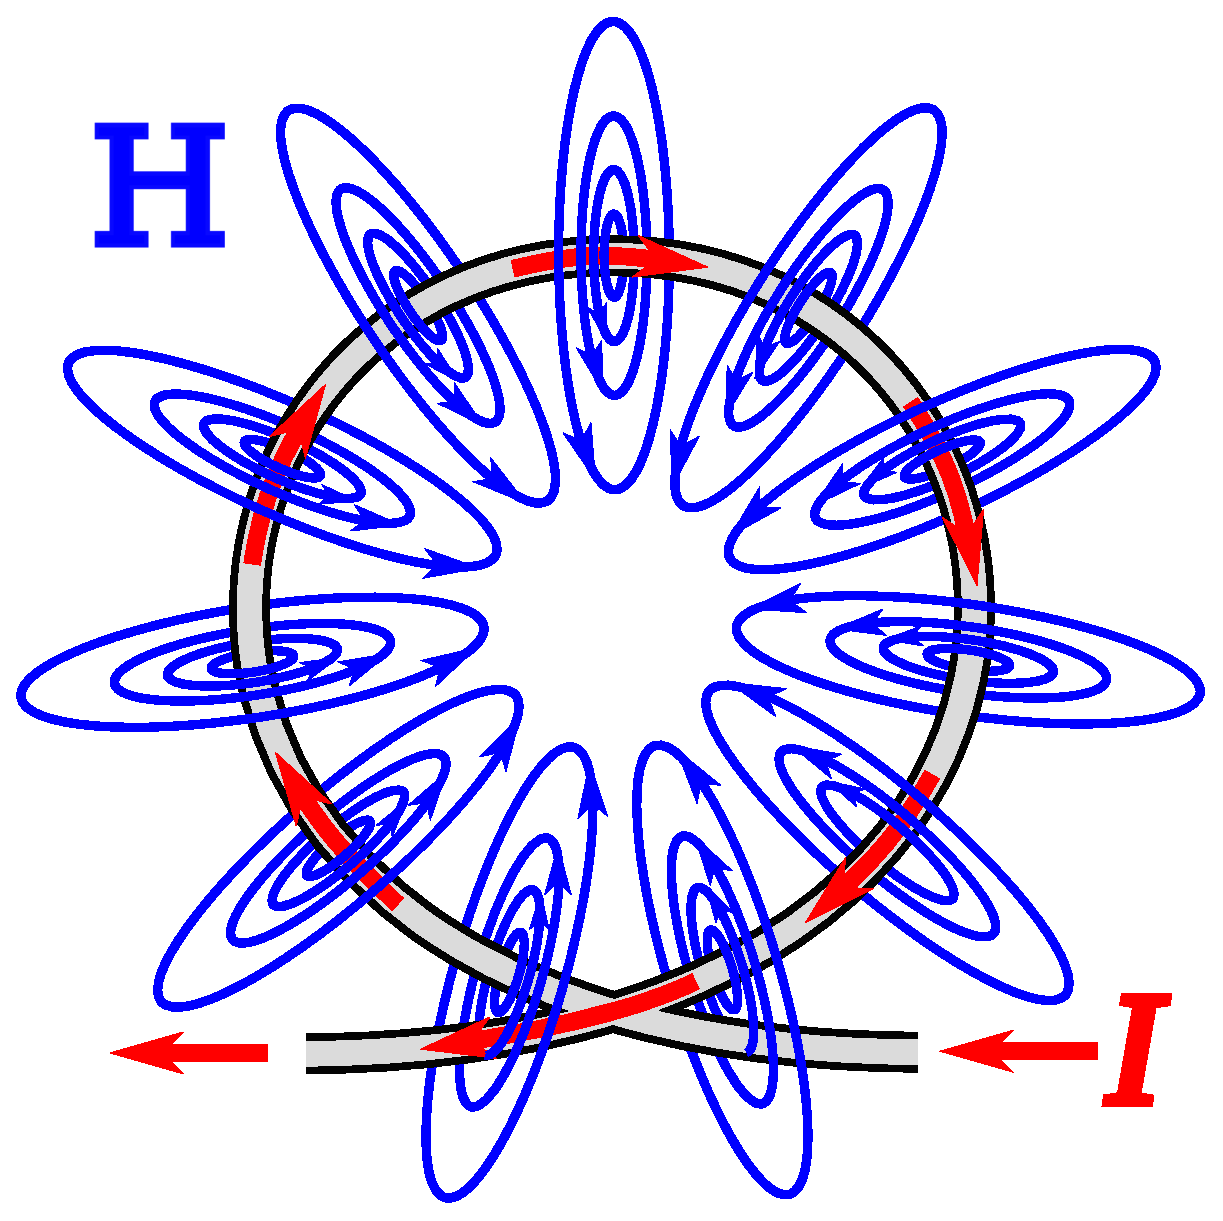
\includegraphics[width=2in]{modules/m0120_fOneTurn.eps}
% https://en.wikipedia.org/wiki/File:Magnetic_field_of_loop_3.svg
}}{A single loop of a coil. A dashed red line moves from the right entrance of the loop, around the loop, and out the left side exit, labeled I. Around the loop are 11 sets of blue concentric circles that represent magnetic fields, labeled H and spaced evenly. Each set has arrows on each concentric circle that point in toward the middle of the loop.}
\end{center} 
\centerline{\scriptsize 
\copyright~\hyperref[m0120_fOneTurn_Credit]{Chetvorno} 
\href{https://creativecommons.org/publicdomain/zero/1.0/deed.en}{CC0 1.0} (modified)
} 
\caption{
\label{m0120_fOneTurn}
Magnetic field due to a single loop.
}
\end{figure} 
 
Figure~\ref{m0120_fStraightCoilFieldLines}
also indicates that the magnetic field lines near the ends of the coil diverge from the axis of the coil.
This is understandable since magnetic field lines form closed loops.
The relatively complex structure of the magnetic fields near the ends of the coil (the ``fringing field'') 
\index{fringing (field)}
and outside of the coil make them relatively difficult to analyze.
Therefore, here we shall restrict our attention to the magnetic field deep inside the coil.
This restriction turns out to be of little consequence as long as $l\gg a$. 

Also, it is apparent from the radial symmetry of the coil that the magnitude of the magnetic field cannot depend on $\phi$.
Putting these findings together, we find that the most general form for the magnetic field intensity deep inside the coil is ${\bf H}\approx\hat{\bf z}H(\rho)$.  
That is, the direction of ${\bf H}$ is $\pm\hat{\bf z}$ and the magnitude of ${\bf H}$ depends, at most, on $\rho$.
In fact, we will soon find with the assistance of ACL that the magnitude of ${\bf H}$ doesn't depend on $\rho$ either.

Here's the relevant form of ACL:
%
\begin{equation}   
\oint_{\mathcal C}{ {\bf H} \cdot d{\bf l} } = I_{encl}  
\label{m0120_eACL}
\end{equation}
%
where $I_{encl}$ is the current enclosed by the closed path ${\mathcal C}$.
ACL works for {\it any} closed path that encloses the current of interest. 
Also, for simplicity, we prefer a path that lies on a constant-coordinate surface.
The selected path is shown in Figure~\ref{m0120_fPath}.
The benefits of this particular path will soon become apparent. 
However, note for now that this particular choice is consistent with the right-hand rule relating the direction of ${\mathcal C}$ to the direction of positive $I$.
That is, when $I$ is positive, the current in the turns of the coil pass through the surface bounded by ${\mathcal C}$ in the same direction as the fingers of the right hand when the thumb is aligned in the indicated direction of ${\mathcal C}$. 
%
\begin{figure}
\begin{center}
\pdftooltip{{  % note double braces
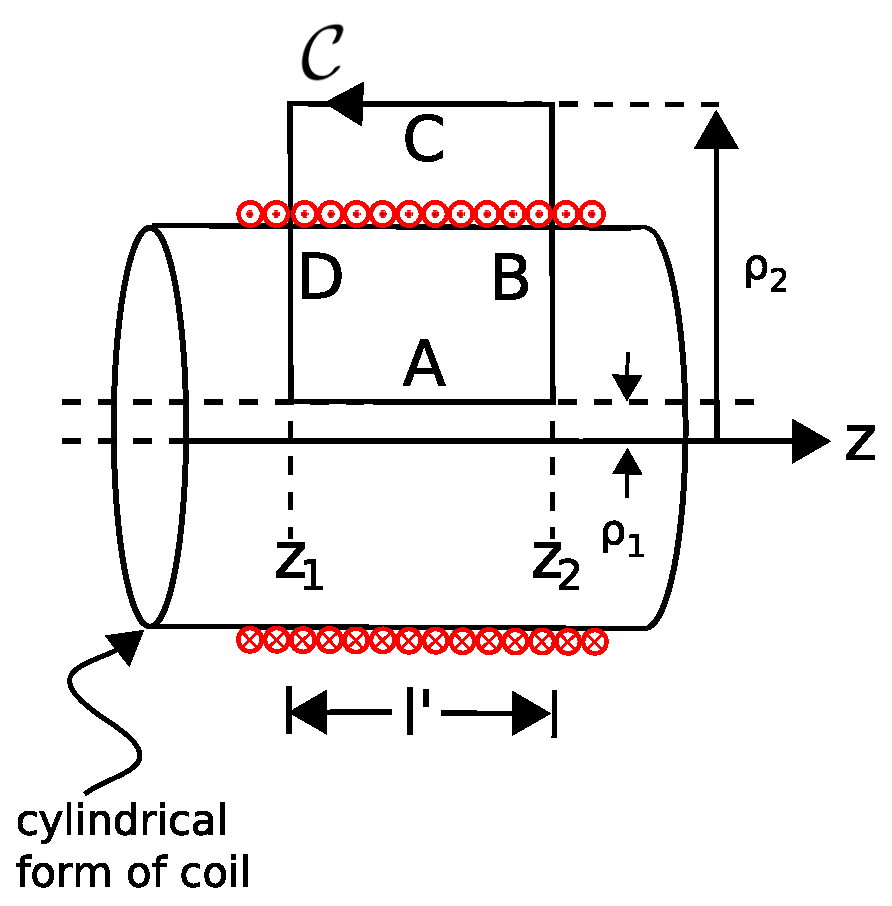
\includegraphics[width=2.5in]{modules/m0120_fPath.eps}
% https://commons.wikimedia.org/wiki/File:M0120_fPath.svg
}}{A cylindrical form of a coil, centered horizontally on the z-axis. On both sides of the cylinder are red circles; the top circles have dots in the middle, and the bottom circles have x’s. Laid over the top half of the cylinder is a square, with sides labeled A (bottom), B, C, and D in a counterclockwise direction creating a closed path, C, with counterclockwise direction. Corner DA is labeled Z sub 1. Corner AB is labeled z sub 2. Length of A is labeled l prime. Distance from z-axis to side C is rho sub 2. distance from z-axis to inner cylinder is rho 1. }
\end{center} 
\centerline{\scriptsize 
\copyright~\hyperref[m0120_fPath_Credit]{K.\ Kikkeri} 
\href{https://creativecommons.org/licenses/by-sa/4.0/}{CC BY~SA 4.0} 
} 
\caption{
\label{m0120_fPath}
Selected path of integration.
}
\end{figure}  

Let's define $N$ to be the number of windings in the coil.
Then, the winding density of the coil is $N/l$ (turns/m).
Let the path length in the $z$ direction be $l'$, as indicated in Figure~\ref{m0120_fPath}.
Then the enclosed current is
%
\begin{equation}
I_{encl}=\frac{N}{l}l'I
\end{equation}
%
That is, the number of turns per unit length times length gives number of turns, and
this quantity times the current through the wire is the total amount of current crossing the surface bounded by ${\mathcal C}$.
 
For the choice of ${\mathcal C}$ made above, and taking our approximation for the form of ${\bf H}$ as exact, Equation~\ref{m0120_eACL} becomes
%
\begin{equation}   
\oint_{\mathcal C}{ \left[\hat{\bf z}H(\rho)\right] \cdot d{\bf l} } = \frac{N}{l}l'I 
\label{m0120_eACL1}
\end{equation}
%
The integral consists of segments $A$, $B$, $C$, and $D$, as shown in Figure~\ref{m0120_fPath}.
Let us consider the result for each of these segments individually:
%
\begin{itemize}
\item The integral over segments $B$ and $D$ is zero because $d{\bf l}=\hat{\rho}d\rho$ for these segments, and so ${\bf H}\cdot d{\bf l}=0$ for these segments.
\item It is also possible to make the contribution from Segment~$C$ go to zero simply by letting $\rho_2\to\infty$.  
The argument is as follows. The magnitude of ${\bf H}$ outside the coil must decrease with distance from the coil, so for $\rho$ sufficiently large, ${\bf H}(\rho)$ becomes negligible.  If that's the case, then the integral over Segment~$C$ also becomes negligible.  
\end{itemize}
%
With $\rho_2\to\infty$, only Segment~$A$ contributes significantly to the integral over ${\mathcal C}$ and Equation~\ref{m0120_eACL1} becomes:
%
\begin{flalign}   
\frac{N}{l}l'I &= \int_{z_1}^{z_2}{ \left[\hat{\bf z}H(\rho_1)\right] \cdot \left(\hat{\bf z}dz\right) } \nonumber \\
               &= H(\rho_1) \int_{z_1}^{z_2}{ dz }                                                       \nonumber \\
               &= H(\rho_1) \left[ z_2-z_1 \right]                                                                    
\label{m0120_eACL2}
\end{flalign}
%
Note $z_2-z_1$ is simply $l'$. 
Also, we have found that the result is independent of $\rho_1$, as anticipated earlier. 
Summarizing:
%
\begin{equation}
\boxed{
{\bf H} \approx \hat{\bf z}\frac{NI}{l} ~~ \mbox{inside coil}
}
\label{m0120_eResult}
\end{equation}

Let's take a moment to consider the implications of this remarkably simple result.
%
\begin{itemize}
\item Note that it is dimensionally correct; that is, current divided by length gives units of A/m, which are the units of ${\bf H}$. 
\item We have found that the magnetic field is simply winding density ($N/l$) times current. To increase the magnetic field, you can either use more turns per unit length or increase the current.
\item We have found that the magnetic field is uniform inside the coil; that is, the magnetic field along the axis is equal to the magnetic field close to the cylinder wall formed by the coil.  However, this does not apply close to ends of the coil, since we have neglected the fringing field. 
\end{itemize}
%
These findings have useful applications in more complicated and practical problems, so it is worthwhile taking note of these now. Summarizing:
%
%ORB HIGHLIGHT
\begin{mdframed}[backgroundcolor=yellow!20,nobreak=true] 
The magnetic field deep inside an ideal straight coil (Equation~\ref{m0120_eResult}) is uniform and proportional to winding density and current.
\end{mdframed}

%------------------------------

{\bf Additional Reading:}
\begin{itemize}
\item ``\href{https://en.wikipedia.org/wiki/Electromagnetic_coil}{Electromagnetic Coil}'' on Wikipedia.
\item ``\href{https://en.wikipedia.org/wiki/Solenoid}{Solenoid}'' on Wikipedia.
\end{itemize}

\index{coil|)}




      \vfill\break
    \section{Magnetic Field of a Toroidal Coil}
{\color{blue}\tiny[m0049]}      % This is text associated with the open textbook "Open Electromagnetics"
% See immediately below for author, date
% This work is licensed under the Creative Commons Attribution-ShareAlike 4.0 International License. (CC BY-SA 4.0) 
% To view a copy of the license, visit http://creativecommons.org/licenses/by-sa/4.0/

%ORB TITLE Magnetic Field of a Toroidal Coil
%ORB AUTHOR 0        # S.W. Ellingson, Virginia Tech (ellingson@vt.edu)
%ORB DATE 20180806   # yyyymmdd
%ORB ABSTRACT Magnetic Field of a toroidal coil

\label{m0049_Magnetic_Field_of_a_Toroidal_Coil} % <-- Must match name of this file and module directory name.  Don't mess with this!
\index{toroidal coil|(}

A toroid 
\index{toroid}
is a cylinder in which the ends are joined to form a closed loop.
An example of a toroidal coil 
\index{coil!toroidal|see{toroidal coil}}
is shown in Figure~\ref{m0049_fToroidalCoilExample}.
Toroidal coils are commonly used to form inductors and transformers.
The principal advantage of toroidal coils over straight coils in these applications is \emph{magnetic field containment} -- as we shall see in this section, the magnetic field outside of a toroidal coil can be made negligibly small.
This reduces concern about interactions between this field and other fields and structures in the vicinity.
%
\begin{figure}[b!]
\begin{center}
\pdftooltip{{  % note double braces
\includegraphics[width=2in]{modules/m0049_fToroidalCoilExample.eps}
% https://en.wikipedia.org/wiki/File:3Com_OfficeConnect_ADSL_Wireless_11g_Firewall_Router_2012-10-28-0869.jpg
}}{A photo of a toroidal coil on a circuit board. Wire is wound on a yellow plastic toroid. Beside the coil are two cylindrical capacitors.}
\end{center} 
\centerline{\scriptsize 
\copyright~\hyperref[m0049_fToroidalCoilExample_Credit]{Slick} 
\href{https://creativecommons.org/publicdomain/zero/1.0/deed.en}{CC0 1.0} 
} 
\caption{
\label{m0049_fToroidalCoilExample}
A toroidal coil used as a large-value inductor in the power supply of a wireless router.
}
\end{figure} 

In this section, we use the magnetostatic form of Ampere's Circuital Law (ACL) 
\index{Ampere's law!magnetostatics}
(Section~\ref{m0019_Amperes_Law_Magnetostatics}) to determine the magnetic field due to a steady (DC) current flowing through a toroidal coil.
The problem is illustrated in Figure~\ref{m0049_fToroidalCoil}.
The toroid is circular with inner and outer radii $a$ and $b$, respectively. %; and with circular cross-section having radius $c=(b-a)/2$.
The coil consists of $N$ windings (turns) of wire wound with uniform winding density.
This problem is easiest to work in cylindrical coordinates with the toroid centered on the origin in $z=0$ plane.
%
\begin{figure}
\begin{center}
\pdftooltip{{  % note double braces
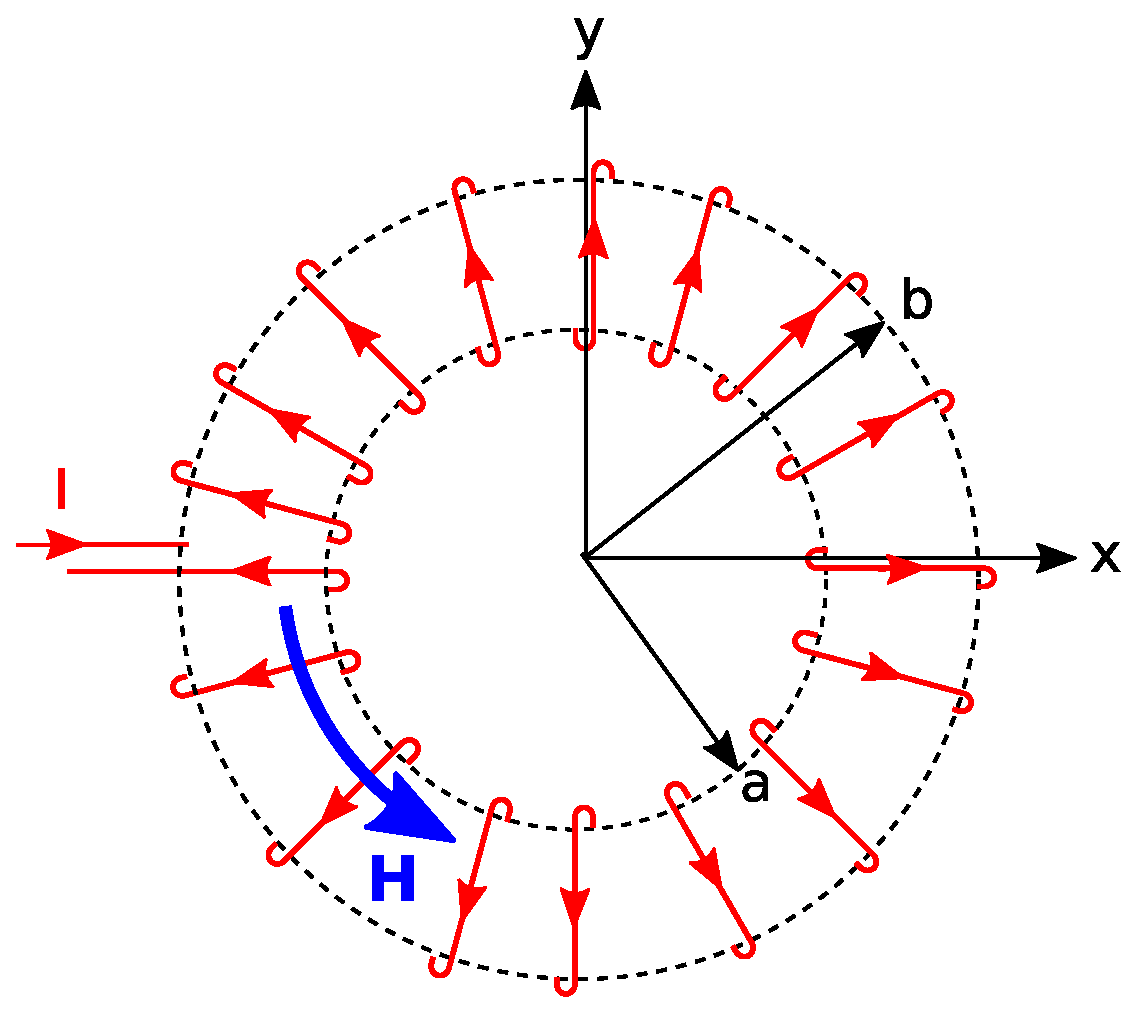
\includegraphics[width=\columnwidth]{modules/m0049_fCoil.eps}
}}{A circular toroidal coil, with the open center at the origin of a xy-axis, with inner radius a and outer radius b. Around the loop the coil is shown as looped arrows, each of which are pointing out away from the center of the coil. From the left, a vector labeled I is pointing toward the coil. H is shown counterclockwise around the loop.}
\end{center} 
% ***WikipediaCommonsURL
%\centerline{\scriptsize 
%\copyright~\hyperref[m0049_fCoil_Credit]{author} 
%\href{https://creativecommons.org/licenses/by-sa/4.0/}{CC BY-SA 4.0} 
%} 
\caption{
\label{m0049_fToroidalCoil}
Geometry of a toroidal coil.
}
\end{figure}  

To begin, let's take stock of what we already know about the answer, which is actually quite a bit.
First, a review of 
Section~\ref{m0120_Magnetic_Field_of_a_Coil} (``Magnetic Field Inside a Straight Coil'') is recommended.
There it is shown that the magnetic field deep inside a straight coil is aligned with axis of the coil.
This can be explained using the result for the magnetic field due to a straight line current (Section~\ref{m0119_Magnetic_Field_of_a_Long_Wire}), in which we found that the magnetic field follows a ``right-hand rule'' -- 
\index{right-hand rule!magnetic field of a wire}
The magnetic field points in the direction of the curled fingers of the right hand when the thumb of the right hand is aligned in the direction of current flow. 
The wire comprising the coil is obviously \emph{not} straight, but we can consider just one short segment of one turn and then sum the results for all such segments.
When we do this, we see that the direction of the magnetic field inside the coil must be in the $+\hat{\bf \phi}$ direction when the current $I$ is applied as shown in Figure~\ref{m0049_fToroidalCoil}.
Also, because the problem is identical after any amount of rotation around the $z$ axis, the magnitude of the magnetic field cannot depend on $\phi$.
Putting these findings together, we find that the most general form for the magnetic field intensity inside or outside the coil is ${\bf H}=\hat{\bf \phi}H(\rho,z)$.  

Here's the relevant form of ACL:
%
\begin{equation}   
\oint_{\mathcal C}{ {\bf H} \cdot d{\bf l} } = I_{encl}  
\label{m0049_eACL}
\end{equation}
%
where $I_{encl}$ is the current enclosed by the closed path ${\mathcal C}$.
ACL works for {\it any} closed path, but we need one that encloses some current so as to obtain a relationship between $I$ and ${\bf H}$.
Also, for simplicity, we prefer a path that lies on a constant-coordinate surface.
The selected path is a circle of radius $\rho$ centered on the origin in the $z=z_0$ plane, as shown in Figure~\ref{m0049_fPath}.
We further require ${\mathcal C}$ to lie entirely inside the coil, which ensures that the enclosed current includes the current of all the windings as they pass through the hole at the center of the toroid.
We choose the direction of integration to be in the $+\phi$ direction, which is consistent with the indicated direction of positive $I$.
That is, when $I$ is positive, the current in the windings of the coil pass through the surface bounded by ${\mathcal C}$ in the same direction as the curled fingers of the right hand when the thumb is aligned in the indicated direction of ${\mathcal C}$. 
%
\begin{figure}
\begin{center}
\pdftooltip{{  % note double braces
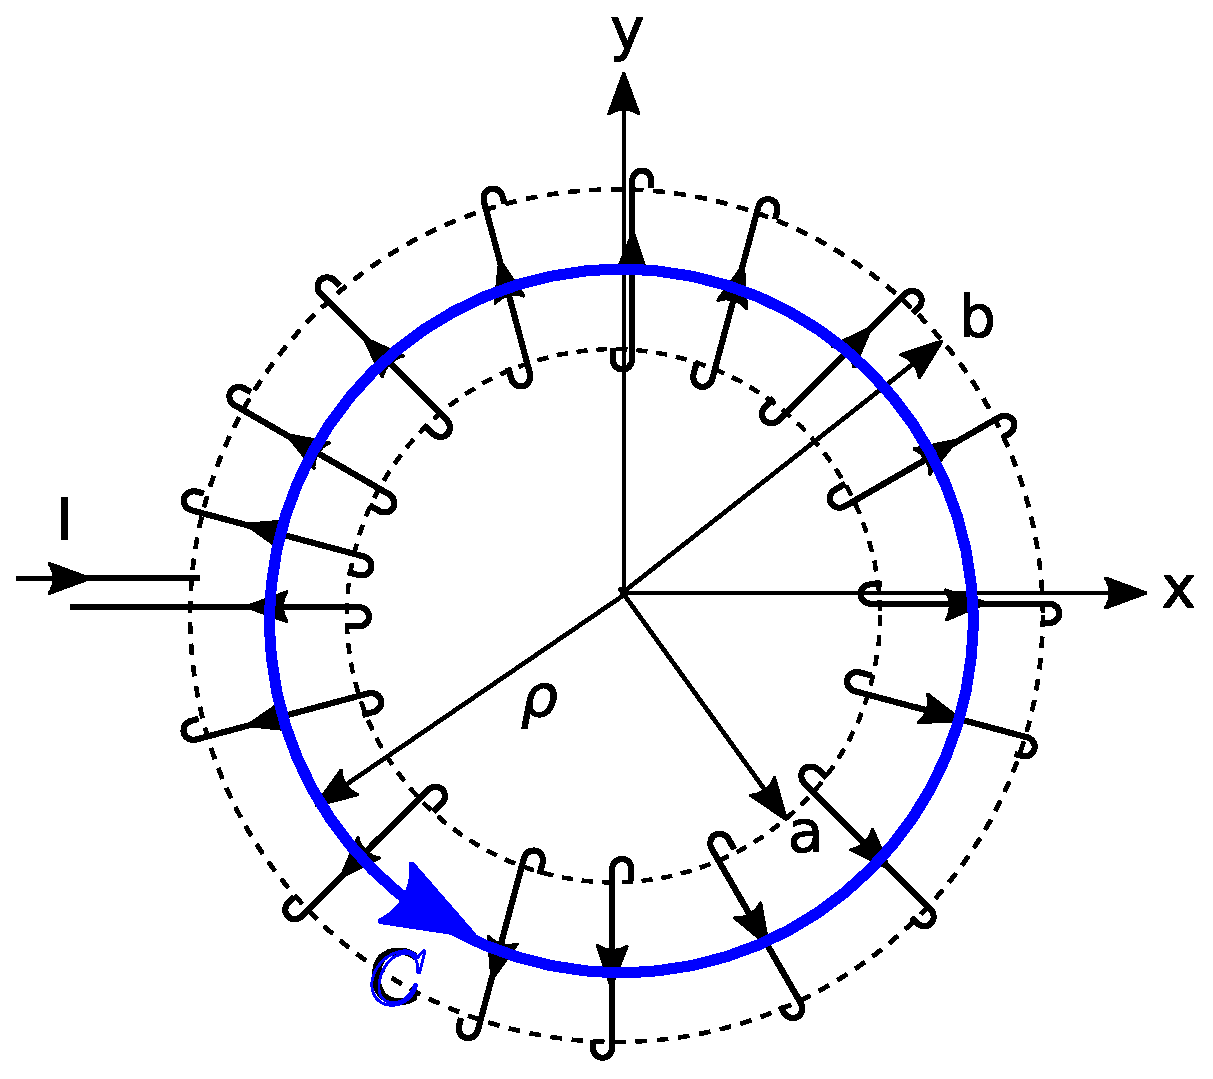
\includegraphics[width=\columnwidth]{modules/m0049_fPath.eps}
}}{A circular toroidal coil, the same as in a previous figure. From the origin pointing toward the bottom left, is a vector labeled rho. A blue circle sits in the middle of the coil, with an arrow pointed in a counterclockwise direction, labeled C.}
\end{center} 
% ***WikipediaCommonsURL
%\centerline{\scriptsize 
%\copyright~\hyperref[m0049_fPath_Credit]{author} 
%\href{https://creativecommons.org/licenses/by-sa/4.0/}{CC BY-SA 4.0} 
%} 
\caption{
\label{m0049_fPath}
Selected path of integration.
}
\end{figure}  

In terms of the variables we have defined, the enclosed current is simply
%
\begin{equation}
I_{encl}=NI
\end{equation}
% 
Equation~\ref{m0049_eACL} becomes
%
\begin{equation}   
\oint_{\mathcal C}{ \left[\hat{\bf \phi}H(\rho,z_0)\right] \cdot d{\bf l} } = NI 
\label{m0049_eACL1}
\end{equation}
%
Now evaluating the integral:
%
\begin{flalign}   
NI &= \int_{0}^{2\pi}{ \left[\hat{\bf \phi}H(\rho,z_0)\right] \cdot \left(\hat{\bf \phi}~\rho~d\phi\right) } \nonumber \\
   &= \rho H(\rho,z_0) \int_{0}^{2\pi}{ d\phi }                                                       \nonumber \\
   &= 2\pi\rho H(\rho,z_0)                                                                   
\label{m0049_eACL2}
\end{flalign}
%
It is now clear that the result is independent of $z_0$. 
Summarizing:
%
\begin{equation}
\boxed{
{\bf H} = \hat{\bf \phi}\frac{NI}{2\pi\rho} ~~ \mbox{inside coil}
}
\label{m0049_eResult}
\end{equation}

Let's take a moment to consider the implications of this result.
%
\begin{itemize}
\item Note that it is dimensionally correct; that is, current divided by the circumference of ${\mathcal C}$ ($2\pi\rho$) gives units of A/m, which are the units of ${\bf H}$. 
\item We have found that the magnetic field is proportional to winding density (i.e., number of windings divided by circumference) times current. To increase the magnetic field you can either use more windings or increase the current.
\item Remarkably, we have found that the magnitude of the magnetic field inside the coil depends only on $\rho$; i.e., the distance from the central (here, $z$) axis.  It is independent of $z$.
\end{itemize}
%
Summarizing:
%
%ORB HIGHLIGHT
\begin{mdframed}[backgroundcolor=yellow!20,nobreak=true] 
The magnetic field inside a toroidal coil (Equation~\ref{m0049_eResult}) depends only on distance from the central axis and is proportional to winding density and current.
\end{mdframed}

Now let us consider what happens outside the coil.  For this, we consider any path of integration (${\mathcal C}$) that lies completely outside the coil.  
Note that any such path encloses no current and therefore $I_{encl}=0$ for any such path.
In this case we have:
%
\begin{equation}   
\oint_{\mathcal C}{ {\bf H} \cdot d{\bf l} } = 0 
\end{equation}
%
There are two ways this could be true.  Either ${\bf H}$ could be zero everywhere along the path, or ${\bf H}$ could be non-zero along the path in such a way that the integral windings out to be zero.  The radial symmetry of the problem rules out the second possibility -- if ${\bf H}$ is radially symmetric and ${\mathcal C}$ is radially symmetric, then the sign of ${\bf H} \cdot d{\bf l}$ should not change over ${\mathcal C}$.  Therefore:
%
%ORB HIGHLIGHT
\begin{mdframed}[backgroundcolor=yellow!20,nobreak=true,nobreak=true] 
The magnetic field everywhere outside an ideal toroidal coil is zero. 
\end{mdframed}
%
Note the caveat signaled by the use of the adjective ``ideal.'' In a practical toroidal coil, we expect there will be some leakage of magnetic flux between the windings.  In practice, this leakage can be made negligibly small by using a sufficiently high winding density and winding the wire on material on a toroidal form (a ``core'') having sufficiently large permeability.  
The use of a high-permeability core, as shown in Figure~\ref{m0049_fToroidalCoilExample}, will dramatically improve the already pretty-good containment.  In fact, the use of such a core allows the spacing between windings to become quite large before leakage becomes significant.

One final observation about toroidal coils is that at no point in the derivation of the magnetic field did we need to consider the cross-sectional shape of the coil; we merely needed to know whether ${\mathcal C}$ was inside or outside the coil.  Therefore:
%
%ORB HIGHLIGHT
\begin{mdframed}[backgroundcolor=yellow!20,nobreak=true] 
The magnetic field inside an ideal toroidal coil does not depend on the cross-sectional shape of the coil. 
\end{mdframed}

%------------------------------

{\bf Additional Reading:}
\begin{itemize}
\item ``\href{https://en.wikipedia.org/wiki/Toroidal_inductors_and_transformers}{Toroidal Inductors and Transformers}'' on Wikipedia.
\end{itemize}

\index{toroidal coil|)}


      \vfill\break
    \section{Magnetic Field of an Infinite Current Sheet}
{\color{blue}\tiny[m0121]}      % This is text associated with the open textbook "Open Electromagnetics"
% See immediately below for author, date
% This work is licensed under the Creative Commons Attribution-ShareAlike 4.0 International License. (CC BY-SA 4.0) 
% To view a copy of the license, visit http://creativecommons.org/licenses/by-sa/4.0/

%ORB TITLE Magnetic Field of an Infinite Current Sheet
%ORB AUTHOR 0        # S.W. Ellingson, Virginia Tech (ellingson@vt.edu)
%ORB DATE 20180628   # yyyymmdd
%ORB ABSTRACT Magnetic Field of an Infinite Current Sheet

\label{m0121_Magnetic_Field_of_an_Infinite_Current_Sheet} % <-- Must match name of this file and module directory name.  Don't mess with this!

We now consider the magnetic field due to an infinite sheet of current, 
\index{current density!surface}
shown in Figure~\ref{m0121_fCurrentSheet}.
The solution to this problem is useful as a building block and source of insight in more complex problems, as well as being a useful approximation to some practical problems involving current sheets of finite extent including, for example, microstrip transmission line and ground plane currents in printed circuit boards.
%
\begin{figure}[b!]
\begin{center}
\pdftooltip{{  % note double braces
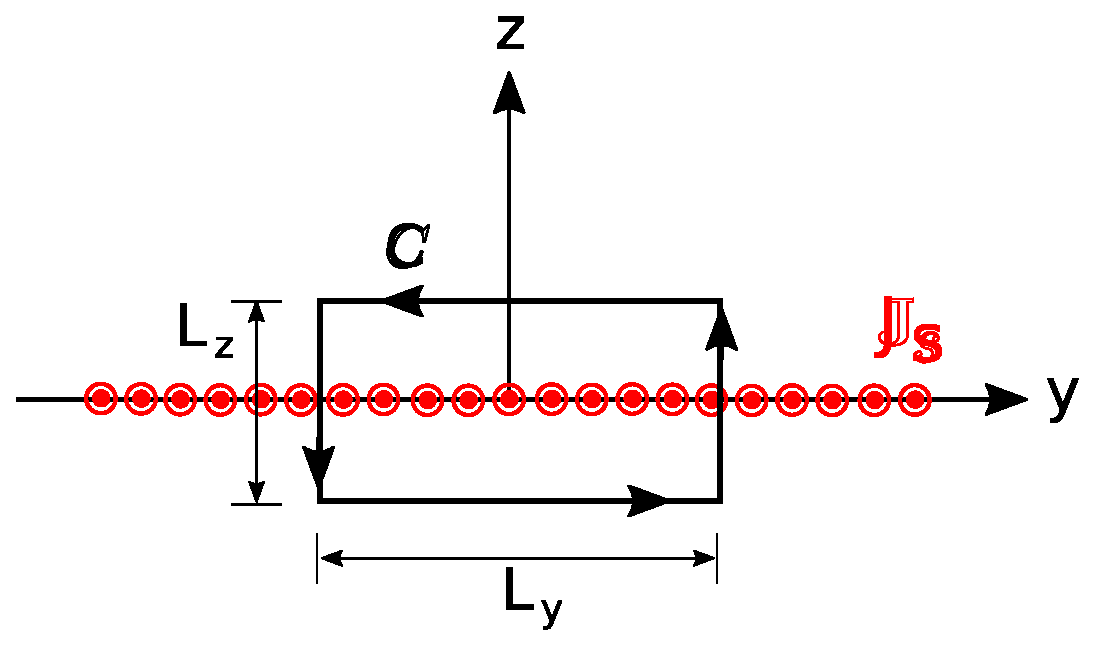
\includegraphics[width=\columnwidth]{modules/m0121_fCurrentSheet.eps}
}}{A rectangle in a closed loop, C, with counterclockwise direction. The z-axis projects perpendicularly from the center of the closed path. Along the y-axis, which runs horizontally through the closed path are red circles with red dots inside labeled J sub s. The closed path has length L sub y and height L sub z. }
\end{center} 
% URL
%\centerline{\scriptsize 
%\copyright~\hyperref[m0121_fCurrentSheet_Credit]{Slick} 
%\href{https://creativecommons.org/publicdomain/zero/1.0/deed.en}{CC0 1.0} 
%} 
\caption{
\label{m0121_fCurrentSheet}
Analysis of the magnetic field due to an infinite thin sheet of current.
}
\end{figure} 

The current sheet in Figure~\ref{m0121_fCurrentSheet} lies in the $z=0$ plane and the current density is ${\bf J}_s = \hat{\bf x}J_s$ (units of A/m); i.e., the current is uniformly distributed such that the total current crossing any segment of width $\Delta y$ along the $y$ direction is $J_s \Delta y$.

To begin, let's take stock of what we already know about the answer, which is actually quite a bit.
For example, imagine the current sheet as a continuum of thin strips parallel to the $x$ axis and very thin in the $y$ dimension.  
Each of these strips individually behaves like a straight line current $I=J_s\Delta y$ (units of A).
The magnetic field due to each of these strips is determined by a ``right-hand rule'' -- 
\index{right-hand rule!magnetic field of a wire}
the magnetic field points in the direction of the curled fingers of the right hand when the thumb of the right hand is aligned in the direction of current flow. (Section~\ref{m0119_Magnetic_Field_of_a_Long_Wire}).
It is apparent from this much that ${\bf H}$ can have no $\hat{\bf y}$ component, since the field of each individual strip has no $\hat{\bf y}$ component.
When the magnetic field due to each strip is added to that of all the other strips, the $\hat{\bf z}$ component of the sum field must be zero due to symmetry.
It is also clear from symmetry considerations that the magnitude of ${\bf H}$ cannot depend on $x$ or $y$. 
Summarizing, we have determined that the most general form for ${\bf H}$ is $\hat{\bf y}H(z)$, and furthermore, the sign of $H(z)$ must be positive for $z<0$ and negative for $z>0$.

It's possible to solve this problem by actually summing over the continuum of thin current strips as imagined above.\footnote{In fact, this is pretty good thing to try, if for no other reason than to see how much simpler it is to use ACL instead.}
However, it's far easier to use Ampere's Circuital Law 
\index{Ampere's law!magnetostatics}
(ACL; Section~\ref{m0019_Amperes_Law_Magnetostatics}).                        
Here's the relevant form of ACL:
%
\begin{equation}   
\oint_{\mathcal C}{ {\bf H} \cdot d{\bf l} } = I_{encl}  
\label{m0121_eACL}
\end{equation}
%
where $I_{encl}$ is the current enclosed by a closed path ${\mathcal C}$.
ACL works for {\it any} closed path, but we need one that encloses some current so as to obtain a relationship between ${\bf J}_s$ and ${\bf H}$.
Also, for simplicity, we prefer a path that lies on a constant-coordinate surface.
A convenient path in this problem is a rectangle lying in the $x=0$ plane and centered on the origin, as shown in Figure~\ref{m0121_fCurrentSheet}.
We choose the direction of integration to be counter-clockwise from the perspective shown in Figure~\ref{m0121_fCurrentSheet}, which is consistent with the indicated direction of positive $J_s$ according to the applicable right-hand rule
\index{right-hand rule!Stokes' theorem}
from Stokes' Theorem.
That is, when $J_s$ is positive (current flowing in the $+\hat{\bf x}$ direction), the current passes through the surface bounded by ${\mathcal C}$ in the same direction as the curled fingers of the right hand when the thumb is aligned in the indicated direction of ${\mathcal C}$. 

Let us define $L_y$ to be the width of the rectangular path of integration in the $y$ dimension and $L_z$ to be the width in the $z$ dimension. 
In terms of the variables we have defined, the enclosed current is simply
%
\begin{equation}
I_{encl}=J_s L_y
\end{equation}
% 
Equation~\ref{m0121_eACL} becomes
%
\begin{equation}   
\oint_{\mathcal C}{ \left[\hat{\bf y}H(z)\right] \cdot d{\bf l} } = J_s L_y
\label{m0121_eACL1}
\end{equation}
%
Note that ${\bf H}\cdot d{\bf l}=0$ for the vertical sides of the path, since ${\bf H}$ is $\hat{\bf y}$-directed and $d{\bf l}=\hat{\bf z}dz$ on those sides.
Therefore, only the horizontal sides contribute to the integral and we have:
%
\begin{flalign}   
~\int_{-L_y/2}^{+L_y/2}{ \left[\hat{\bf y}H\left(-\frac{L_z}{2}\right)\right] \cdot \left(\hat{\bf y}dy\right) } & ~ \nonumber \\
+\int_{+L_y/2}^{-L_y/2}{ \left[\hat{\bf y}H\left(+\frac{L_z}{2}\right)\right] \cdot \left(\hat{\bf y}dy\right) } &= J_s L_y
\end{flalign}
%
Now evaluating the integrals:
%
\begin{equation} 
H\left(-\frac{L_z}{2}\right)~L_y - H\left(+\frac{L_z}{2}\right)~L_y = J_s L_y
\end{equation}
%
Note that all factors of $L_y$ cancel in the above equation.
Furthermore, $H(-L_z/2)=-H(+L_z/2)$ due to (1) symmetry between the upper and lower half-spaces and (2) the change in sign between these half-spaces, noted earlier.
We use this to eliminate $H(+L_z/2)$ and solve for $H(-L_z/2)$ as follows:
%
\begin{equation} 
2 H(-L_z/2) = J_s 
\end{equation}
%
yielding
%
\begin{equation} 
H(-L_z/2) = +\frac{J_s}{2}
\end{equation}
%
and therefore
%
\begin{equation} 
H(+L_z/2) = -\frac{J_s}{2}
\end{equation}
%
Furthermore, note that ${\bf H}$ is independent of $L_z$; for example, the result we just found indicates the same value of $H(+L_z/2)$ regardless of the value of $L_z$.
Therefore, ${\bf H}$ is uniform throughout all space, except for the change of sign corresponding for the field above vs.\ below the sheet.
Summarizing:
%
\begin{equation} 
\boxed{
{\bf H} = \pm\hat{\bf y}\frac{J_s}{2}~~\mbox{for}~z\lessgtr 0
}
\label{m0121_eResult}
\end{equation}

%ORB HIGHLIGHT
\begin{mdframed}[backgroundcolor=yellow!20,nobreak=true] 
The magnetic field intensity due to an infinite sheet of current (Equation~\ref{m0121_eResult}) is spatially uniform except for a change of sign corresponding for the field above vs.\ below the sheet.
\end{mdframed}


      \vfill\break
    \section{Ampere's Law (Magnetostatics): Differential Form}
{\color{blue}\tiny[m0118]}      % This is text associated with the open textbook "Open Electromagnetics"
% See immediately below for author, date
% This work is licensed under the Creative Commons Attribution-ShareAlike 4.0 International License. (CC BY SA 4.0) 
% To view a copy of the license, visit http://creativecommons.org/licenses/by-sa/4.0/

%ORB TITLE Ampere's Law (Magnetostatics): Differential Form 
%ORB AUTHOR 0        # S.W. Ellingson, Virginia Tech (ellingson@vt.edu)
%ORB DATE 20180806   # yyyymmdd
%ORB ABSTRACT Ampere's Law (Magnetostatics): Differential Form from Integral Form

\label{m0118_Amperes_Law_Magnetostatics_Integral-to-Differential} % <-- Must match name of this file and module directory name.  Don't mess with this!

The integral form of Amperes' Circuital Law 
\index{Ampere's law!magnetostatics}
(ACL; Section~\ref{m0019_Amperes_Law_Magnetostatics}) for magnetostatics relates the magnetic field along a closed path to the total current flowing through any surface bounded by that path.
In mathematical form:
%
\begin{equation}
\oint_{\mathcal C}{ {\bf H} \cdot d{\bf l} } = I_{encl}  
\end{equation}
%
where ${\bf H}$ is magnetic field intensity, ${\mathcal C}$ is the closed curve, and $I_{encl}$ is the total current flowing through any surface bounded by ${\mathcal C}$.
In this section, we derive the differential form of this equation.
In some applications, this differential equation, combined with boundary conditions associated with discontinuities in structure and materials, can be used to solve for the magnetic field in arbitrarily complicated scenarios.  
A more direct reason for seeking out this differential equation is that we gain a little more insight into the relationship between current and the magnetic field, disclosed at the end of this section.

The equation we seek may be obtained using Stokes' Theorem (Section~\ref{m0051_Stokes_Theorem}), which in the present case may be written:
%
\begin{equation}   
\int_{\mathcal S} \left( \nabla \times {\bf H} \right) \cdot d{\bf s} = \oint_{\mathcal C} {\bf H}\cdot d{\bf l}
\label{m0118_eACL2}
\end{equation}
%
where ${\mathcal S}$ is any surface bounded by ${\mathcal C}$, and $d{\bf s}$ is the differential surface area combined with the unit vector in the direction determined by the right-hand rule from Stokes' Theorem.
\index{right-hand rule!Stokes' theorem}
ACL tells us that the right side of the above equation is simply $I_{encl}$.
We may express $I_{encl}$ as the integral of the volume current density ${\bf J}$ (units of A/m$^2$; Section~\ref{m0101_Current_Distributions}) as follows:
%
\begin{equation}
I_{encl} = \int_{\mathcal S} {\bf J} \cdot d{\bf s}
\end{equation}
%
so we may rewrite Equation~\ref{m0118_eACL2} as follows:
%
\begin{equation}   
\int_{\mathcal S} \left( \nabla \times {\bf H} \right) \cdot d{\bf s} = \int_{\mathcal S} {\bf J} \cdot d{\bf s}
\end{equation}
%
The above relationship must hold regardless of the specific location or shape of ${\mathcal S}$.  The only way this is possible for all possible surfaces in all applicable scenarios is if the integrands are equal.  Thus, we obtain the desired expression:
%
\begin{equation}
\boxed{
\nabla \times {\bf H} = {\bf J}
}
\label{m0118_eACL}
\end{equation}
%
That is, the curl of the magnetic field intensity at a point is equal to the volume current density at that point.  
Recalling the properties of the curl operator (Section~\ref{m0048_Curl}) -- in particular, that curl involves derivatives with respect to direction -- we conclude:
%
%ORB HIGHLIGHT
\begin{mdframed}[backgroundcolor=yellow!20,nobreak=true] 
The differential form of Ampere's Circuital Law for magnetostatics (Equation~\ref{m0118_eACL}) indicates that the volume current density at any point in space is proportional to the spatial rate of change of the magnetic field and is perpendicular to the magnetic field at that point.
\end{mdframed}

%-------------------------------------------------------

{\bf Additional Reading:}
\begin{itemize}
\item ``\href{https://en.wikipedia.org/wiki/Ampere's_circuital_law}{Ampere's circuital law}'' on Wikipedia.
\item ``\href{https://en.wikipedia.org/wiki/Boundary_value_problem}{Boundary value problem}'' on Wikipedia.
\end{itemize}




      \vfill\break
    \section{Boundary Conditions on the Magnetic Flux Density ({\bf B})}
{\color{blue}\tiny[m0022]}      % This is text associated with the open textbook "Open Electromagnetics"
% See immediately below for author, date
% This work is licensed under the Creative Commons Attribution-ShareAlike 4.0 International License. (CC BY SA 4.0) 
% To view a copy of the license, visit http://creativecommons.org/licenses/by-sa/4.0/

%ORB TITLE Boundary Conditions on the Magnetic Flux Density ({\bf B}) 
%ORB AUTHOR 0        # S.W. Ellingson, Virginia Tech (ellingson@vt.edu)
%ORB DATE 20180806   # yyyymmdd
%ORB ABSTRACT Boundary Conditions on the Magnetic Flux Density

\label{m0022_Boundary_Conditions_on_B} % <-- Must match name of this file and module directory name.  Don't mess with this!

In homogeneous media, electromagnetic quantities vary smoothly and continuously.
At an interface between dissimilar media, however, it is possible for electromagnetic quantities to be discontinuous.
Continuities and discontinuities in fields can be described mathematically by \emph{boundary conditions} 
\index{boundary conditions}
and used to constrain solutions for fields away from these interfaces.

In this section, we derive the boundary condition on the magnetic flux density ${\bf B}$ at a smooth interface between two material regions, as shown in Figure~\ref{m0022_fBoundary}.\footnote{It may be helpful to note the similarity (duality, in fact) between this derivation and the derivation of the associated boundary condition on ${\bf D}$ presented in Section~\ref{m0021_Boundary_Conditions_on_D}.} 
%
\begin{figure}[b!]
\begin{center}
\pdftooltip{{  % note double braces
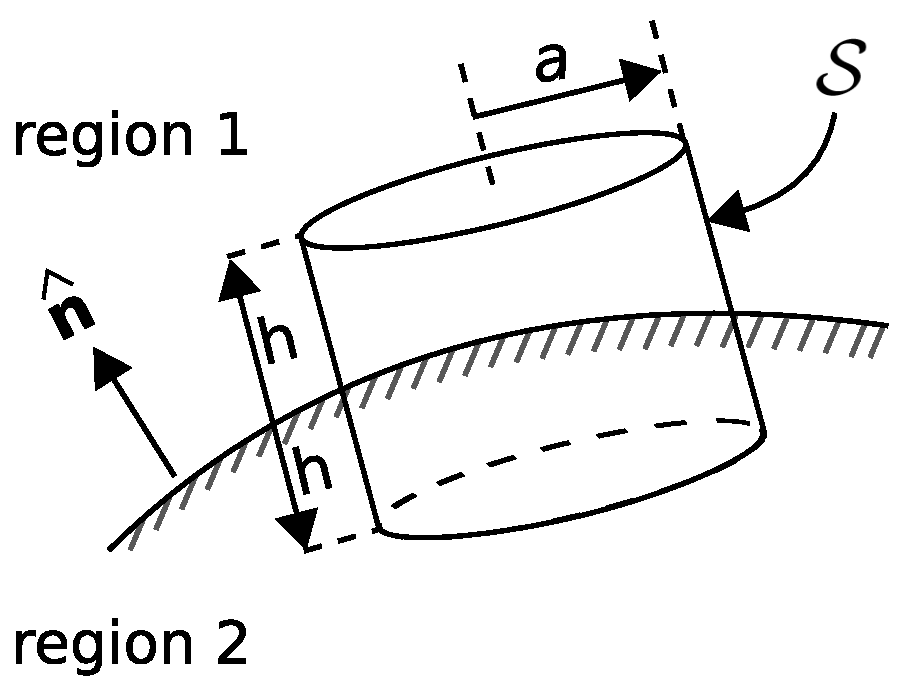
\includegraphics[width=2in]{modules/m0022_fBoundary.eps}
% https://commons.wikimedia.org/wiki/File:M0022_fBoundary.svg
}}{A closed cylinder with surface, S, is centered at a point on an interface. The flat ends are parallel to the surface and n-hat extends perpendicular to the surface. The radius of the cylinder is a, and the hight is h. The region outside the interface is labeled region 1, and the inner is labeled region 2. }
\end{center} 
\centerline{\scriptsize 
\copyright~\hyperref[m0022_fBoundary_Credit]{K.\ Kikkeri} 
\href{https://creativecommons.org/licenses/by-sa/4.0/}{CC BY~SA 4.0} 
} 
\caption{
\label{m0022_fBoundary}
Determination of the boundary condition on ${\bf B}$ at the interface between material regions.
}
\end{figure}
%
The desired boundary condition may be obtained from Gauss' Law for Magnetic Fields (GLM; Section~\ref{m0018_Gauss_Law_Magnetic_Integral_Form}):
%
\begin{equation}
\oint_{\mathcal S} {\bf B}\cdot d{\bf s} = 0
\end{equation}
%
where ${\mathcal S}$ is any closed surface.
Let ${\mathcal S}$ take the form of cylinder centered at a point on the interface, and for which the flat ends are parallel to the surface and perpendicular to $\hat{\bf n}$, as shown in Figure~\ref{m0022_fBoundary}.  
Let the radius of this cylinder be $a$, and let the length of the cylinder be $2h$.  From GLM, we have
%
\begin{align}
\oint_{\mathcal S}{ {\bf B} \cdot d{\bf s} } &= \int_{top} { {\bf B} \cdot d{\bf s} } &            \nonumber \\
                                                 &+ \int_{side} { {\bf B} \cdot d{\bf s} } &            \nonumber \\
                                                 &+ \int_{bottom} { {\bf B} \cdot d{\bf s} } &= 0
\end{align}
% 
Now let us reduce $h$ and $a$ together while (1) maintaining a constant ratio $h/a\ll 1$ and (2) keeping $\mathcal{S}$ centered on the interface.
Because $h\ll a$, the area of the side can be made negligible relative to the area of the top and bottom.
Then, as $h\to 0$, we are left with    
%
\begin{equation}
\int_{top} { {\bf B} \cdot d{\bf s} } + \int_{bottom} { {\bf B} \cdot d{\bf s} }  \to 0
\end{equation}
%
As the area of the top and bottom sides become infinitesimal, the variation in ${\bf B}$ over these areas becomes negligible.  Now we have simply:  
%
\begin{equation}
{\bf B}_1 \cdot \hat{\bf n}\Delta A + {\bf B}_2 \cdot \left( -\hat{\bf n} \right) \Delta A \to 0
\end{equation}
%
where ${\bf B}_1$ and ${\bf B}_2$ are the magnetic flux densities at the interface but in regions~1 and 2, respectively,
and $\Delta A$ is the area of the top and bottom sides.  
Note that the orientation of $\hat{\bf n}$ is important -- we have assumed $\hat{\bf n}$ points into region~1, and we must now stick with this choice.
Thus, we obtain 
%
\begin{equation}
\boxed{
\hat{\bf n} \cdot \left( {\bf B}_1 - {\bf B}_2 \right) = 0
}
\label{m0022_eBCB}
\end{equation}       
%
where, as noted above, $\hat{\bf n}$ points into region~1.

Summarizing:
%
%ORB HIGHLIGHT
\begin{mdframed}[backgroundcolor=yellow!20,nobreak=true] 
The normal (perpendicular) component of ${\bf B}$ across the boundary between two material regions is continuous.
\end{mdframed}

It is worth noting what this means for the magnetic field intensity ${\bf H}$. Since ${\bf B}=\mu{\bf H}$, it must be that
%
%ORB HIGHLIGHT
\begin{mdframed}[backgroundcolor=yellow!20,nobreak=true] 
The normal (perpendicular) component of ${\bf H}$ across the boundary between two material regions is discontinuous if the permeabilities are unequal.
\end{mdframed}





      \vfill\break
    \section{Boundary Conditions on the Magnetic Field Intensity ({\bf H})}
{\color{blue}\tiny[m0023]}      % This is text associated with the open textbook "Open Electromagnetics"
% See immediately below for author, date
% This work is licensed under the Creative Commons Attribution-ShareAlike 4.0 International License. (CC BY SA 4.0) 
% To view a copy of the license, visit http://creativecommons.org/licenses/by-sa/4.0/

%ORB TITLE Boundary Conditions on the Magnetic Field Intensity ({\bf H}) 
%ORB AUTHOR 0        # S.W. Ellingson, Virginia Tech (ellingson@vt.edu)
%ORB DATE 20180630   # yyyymmdd
%ORB ABSTRACT Boundary Conditions on the Magnetic Field Intensity

\label{m0023_Boundary_Conditions_on_H} % <-- Must match name of this file and module directory name.  Don't mess with this!

In homogeneous media, electromagnetic quantities vary smoothly and continuously.
At a boundary between dissimilar media, however, it is possible for electromagnetic quantities to be discontinuous.
Continuities and discontinuities in fields can be described mathematically by \emph{boundary conditions}
\index{boundary conditions}
and used to constrain solutions for fields away from these boundaries.
In this section, we derive boundary conditions on the magnetic field intensity ${\bf H}$.

To begin, consider a region consisting of only two media that meet at a smooth boundary as shown in Figure~\ref{m0023_fBoundary}.
%
\begin{figure}[b!]
\begin{center}
\pdftooltip{{  % note double braces
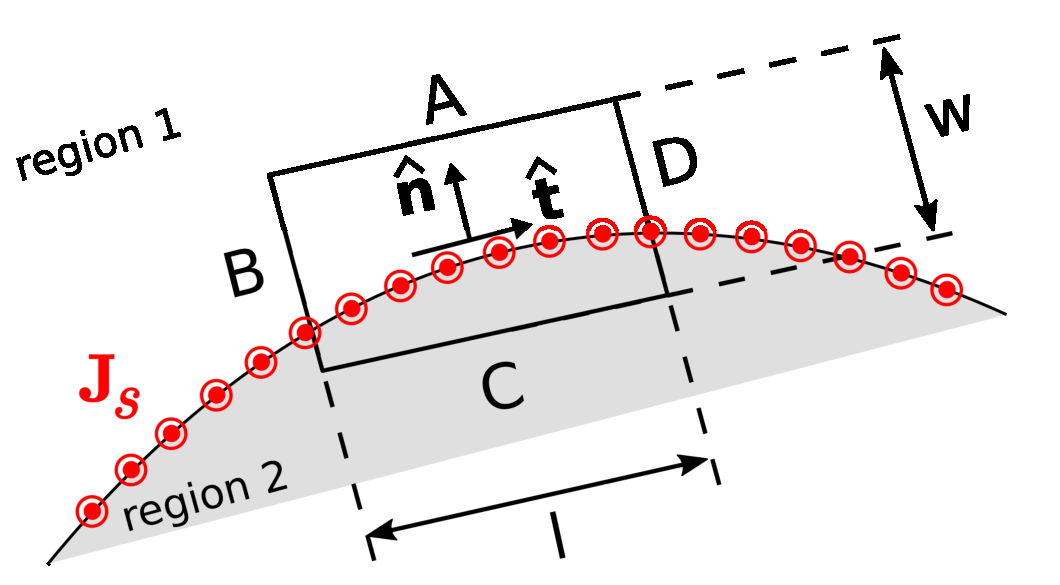
\includegraphics[width=2.5in]{modules/m0023_fBoundary.eps}
}}{A rectangle labeled A, B, C, D (counter-clockwise from the top) centered at a point on a boundary. The long sides of the rectangles are parallel to the surface. The length of the rectangle is l, and the width is w. A vector, t-hat, is tangent to the surface of the boundary. Another vector, n-hat, is perpendicular to the surface of the boundary. On the surface are blue circles with dots in the middle, labeled J sub s. The outer region of the boundary is labeled region 1, and the inner is labeled region 2.}
\end{center} 
% ***WikipediaCommonsURL
%\centerline{\scriptsize 
%\copyright~\hyperref[m0023_fBoundary_Credit]{author} 
%\href{https://creativecommons.org/licenses/by-sa/4.0/}{CC BY~SA 4.0} 
%} 
\caption{
\label{m0023_fBoundary}
Determining the boundary condition on ${\bf H}$ at the smooth boundary between two material regions.
}
\end{figure}
%
The desired boundary condition can be obtained directly from Ampere's Circuital Law (ACL; Section~\ref{m0019_Amperes_Law_Magnetostatics}):
% 
\begin{equation}  
\oint_{\mathcal C}{ {\bf H} \cdot d{\bf l} } = I_{encl}
\label{m0023_eACL}
\end{equation}
% 
where ${\mathcal C}$ is any closed path and $I_{encl}$ is the current that flows through the surface bounded by that path in the direction specified by the ``right-hand rule'' 
\index{right-hand rule!Stokes' theorem}
of Stokes' theorem.
Let ${\mathcal C}$ take the form of a rectangle centered on a point on the boundary as shown in Figure~\ref{m0023_fBoundary}, perpendicular to the direction of current flow at that location.
Let the sides $A$, $B$, $C$, and $D$ be perpendicular and parallel to the boundary.  
Let the length of the parallel sides be $l$, and let the length of the perpendicular sides be $w$.  
Now we apply ACL.  
We must integrate in a counter-clockwise direction in order to be consistent with the indicated reference direction for ${\bf J}_s$.
\index{right-hand rule!Stokes' theorem}
Thus:
% 
\begin{align}   
\oint{ {\bf H} \cdot d{\bf l} } &=\int_A{ {\bf H} \cdot d{\bf l} } & \nonumber \\ 
                                &+\int_B{ {\bf H} \cdot d{\bf l} }  & \nonumber \\ 
                                &+\int_C{ {\bf H} \cdot d{\bf l} }  & \nonumber \\
                                &+\int_D{ {\bf H} \cdot d{\bf l} }  &= I_{encl} 
\end{align}
%  
Now we let $w$ and $l$ become vanishingly small while (1) maintaining the ratio $l/w$ and (2) keeping $\mathcal{C}$ centered on the boundary.
In this process, the contributions from the $B$ and $D$ segments become equal in magnitude but opposite in sign; i.e., 
% 
\begin{equation}   
\int_B{ {\bf H} \cdot d{\bf l} } 
+\int_D{ {\bf H} \cdot d{\bf l} }
\to 0
\end{equation}
%
This leaves
% 
\begin{equation}   
\int_A{ {\bf H} \cdot d{\bf l} } 
+\int_C{ {\bf H} \cdot d{\bf l} }
\to I_{encl}
\end{equation}
%
Let us define the unit vector $\hat{\bf t}$ (``tangent'') as shown in Figure~\ref{m0023_fBoundary}.
Now we have simply: 
% 
\begin{equation}   
  {\bf H}_1 \cdot \left(-\hat{\bf t}\Delta l\right)
+ {\bf H}_2 \cdot \left(+\hat{\bf t}\Delta l\right) 
= I_{encl} 
\label{m0023_eACL2}
\end{equation}
%
where ${\bf H}_1$ and ${\bf H}_2$ are the fields evaluated on the two sides of the boundary, and
$\Delta l \to 0$ is the length of sides $A$ and $C$.
As always, $I_{encl}$ (units of A) may be interpreted as the flux
\index{flux}
of the current density ${\bf J}_s$ (units of A/m) flowing past a line on the surface having length $\Delta l$ (units of m) perpendicular to $\hat{\bf t}\times\hat{\bf n}$, where $\hat{\bf n}$ is the normal to the surface, pointing into Region~1.  Stated mathematically:
%
\begin{equation}
I_{encl} \rightarrow {\bf J}_s \cdot \left( \Delta l ~ \hat{\bf t}\times\hat{\bf n} \right)
\end{equation}
% 
Before proceeding, note this is true regardless of the particular direction we selected for $\hat{\bf t}$; it is only necessary that $\hat{\bf t}$ be tangent to the boundary. Thus, $\hat{\bf t}\times\hat{\bf n}$ need not necessarily be in the same direction as ${\bf J}_s$.
%
Now Equation~\ref{m0023_eACL2} can be written:
% 
\begin{equation}   
  {\bf H}_2 \cdot       \hat{\bf t}                        \Delta l
- {\bf H}_1 \cdot       \hat{\bf t}                        \Delta l 
= {\bf J}_s \cdot \left(\hat{\bf t}\times\hat{\bf n}\right)\Delta l
\end{equation}
%
Eliminating the common factor of $\Delta l$ and arranging terms on the left:
% 
\begin{equation}   
 \left( {\bf H}_2 -{\bf H}_1 \right) \cdot \hat{\bf t} = {\bf J}_s \cdot \left(\hat{\bf t}\times\hat{\bf n}\right)
\label{m0023_eACL3}
\end{equation}
%
The right side may be transformed using a vector identity (Equation~\ref{m0140_eVI1} of Section~\ref{m0140_Vector_Identities}) to obtain:
% 
\begin{equation}   
\left( {\bf H}_2 -{\bf H}_1 \right) \cdot \hat{\bf t} = \hat{\bf t} \cdot \left( \hat{\bf n} \times {\bf J}_s \right)
\label{m0023_eBC1}
\end{equation}
%
%Now recall our earlier statement about the direction of $\hat{\bf t}$.
%; in other words, this must be true for \emph{any} unit vector that is tangent to the surface, and not just for $\hat{\bf t}$ directed as shown in Figure~\ref{m0023_fBoundary}.
Equation~\ref{m0023_eBC1} is the boundary condition we seek.  
We have found that the component of ${\bf H}_2 -{\bf H}_1$ (the difference between the magnetic field intensities at the boundary) in any direction tangent to the boundary is equal to the component of the current density flowing in the perpendicular direction $\hat{\bf n} \times {\bf J}_s$.  Said differently: 
%
%ORB HIGHLIGHT
\begin{mdframed}[backgroundcolor=yellow!20,nobreak=true] 
A discontinuity in the tangential component of the magnetic field intensity at the boundary must be supported by surface current flowing in a direction perpendicular to this component of the field.
\end{mdframed}
%
An important consequence is that:
%
%ORB HIGHLIGHT
\begin{mdframed}[backgroundcolor=yellow!20,nobreak=true] 
If there is no surface current, then the tangential component of the magnetic field intensity is continuous across the boundary.
\end{mdframed}

It is possible to obtain a mathematical form of the boundary condition that is more concise and often more useful than Equation~\ref{m0023_eBC1}.
This form may be obtained as follows.
First, we note that the dot product with respect to $\hat{\bf t}$ on both sides of Equation~\ref{m0023_eBC1} means simply ``any component that is tangent to the boundary.''  We need merely to make sure we are comparing the same tangential component on each side of the equation.  
For example $\hat{\bf n} \times \left( {\bf H}_2 -{\bf H}_1 \right)$ is tangential to the boundary, since $\hat{\bf n}$ is perpendicular to the boundary and therefore any cross product involving $\hat{\bf n}$ will be perpendicular to $\hat{\bf n}$.
The corresponding component of the current density is $\hat{\bf n} \times \left( \hat{\bf n} \times {\bf J}_s \right)$, so Equation~\ref{m0023_eBC1} may be equivalently written as follows: 
% 
\begin{equation}   
\hat{\bf n} \times \left( {\bf H}_2 -{\bf H}_1 \right)  = \hat{\bf n} \times \hat{\bf n} \times {\bf J}_s 
\label{m0023_eBC2}
\end{equation}
%
Applying a vector identity (Equation~\ref{m0140_eVI2} of Section~\ref{m0140_Vector_Identities}) to the right side of Equation~\ref{m0023_eBC2} we obtain: 
%
\begin{align}   
\hat{\bf n} \times \hat{\bf n} \times {\bf J}_s 
     &= \hat{\bf n} \left(\hat{\bf n}\cdot{\bf J}_s\right) - {\bf J}_s\left(\hat{\bf n}\cdot\hat{\bf n}\right) \nonumber \\
     &= \hat{\bf n} \left(0\right) - {\bf J}_s\left(1\right) \nonumber \\
     &= -{\bf J}_s
\end{align}
%
Therefore:
% 
\begin{equation}   
\hat{\bf n} \times \left( {\bf H}_2 -{\bf H}_1 \right)  = -{\bf J}_s
\end{equation}
%
The minus sign on the right can be eliminated by swapping ${\bf H}_2$ and ${\bf H}_1$ on the left, yielding
% 
\begin{equation}   
\boxed{
 \hat{\bf n} \times \left( {\bf H}_1 -{\bf H}_2 \right) = {\bf J}_s                                              
}
\end{equation}
%
This is the form in which the boundary condition is most commonly expressed.

It is worth noting what this means for the magnetic field intensity ${\bf B}$. Since ${\bf B}=\mu{\bf H}$:
%
%ORB HIGHLIGHT
\begin{mdframed}[backgroundcolor=yellow!20,nobreak=true] 
In the absence of surface current, the tangential component of ${\bf B}$ across the boundary between two material regions is discontinuous if the permeabilities are unequal.
\end{mdframed}


      \vfill\break
    \section{Inductance}
{\color{blue}\tiny[m0123]}      % This is text associated with the open textbook "Open Electromagnetics"
% See immediately below for author, date
% This work is licensed under the Creative Commons Attribution-ShareAlike 4.0 International License. (CC BY SA 4.0) 
% To view a copy of the license, visit http://creativecommons.org/licenses/by-sa/4.0/

%ORB TITLE Inductance
%ORB AUTHOR 0        # S.W. Ellingson, Virginia Tech (ellingson@vt.edu)
%ORB DATE 20180806   # yyyymmdd
%ORB ABSTRACT Inductance

\label{m0123_Inductance} % <-- Must match name of this file and module directory name.  Don't mess with this!
\index{inductance|(}

Current creates a magnetic field, which subsequently exerts force on other current-bearing structures.
For example, the current in each winding of a coil exerts a force on every other winding of the coil.
If the windings are fixed in place, then this force is unable to do work (i.e., move the windings), so instead the coil stores potential energy.
This potential energy can be released by turning off the external source.
When this happens, charge continues to flow, but is now propelled by the magnetic force.  
The potential energy that was stored in the coil is converted to kinetic energy and subsequently used to redistribute the charge until no current flows.
At this point, the inductor has expended its stored energy.
To restore energy, the external source must be turned back on, restoring the flow of charge and thereby restoring the magnetic field.
 
Now recall that the magnetic field is essentially defined in terms of the force associated with this potential energy; i.e., ${\bf F} = q{\bf v} \times {\bf B}$ where $q$ is the charge of a particle comprising the current, ${\bf v}$ is the velocity of the particle, and ${\bf B}$ is magnetic flux density (Section~\ref{m0003_Magnetic_Flux_Density}).
So, rather than thinking of the potential energy of the system as being associated with the magnetic force applied to current, it is equally valid to think of the potential energy as being stored in the magnetic field associated with the current distribution.
The energy stored in the magnetic field depends on the geometry of the current-bearing structure and the permeability of the intervening material because the magnetic field depends on these parameters. 

The relationship between current applied to a structure and the energy stored in the associated magnetic field is what we mean by \emph{inductance}.
We may fairly summarize this insight as follows:
%
%ORB HIGHLIGHT
\begin{mdframed}[backgroundcolor=yellow!20,nobreak=true] 
Inductance 
\index{inductance!definition}
is the ability of a structure to store energy in a magnetic field.
\end{mdframed}
%
%ORB HIGHLIGHT
\begin{mdframed}[backgroundcolor=yellow!20,nobreak=true] 
The inductance of a structure depends on the geometry of its current-bearing structures and the permeability of the intervening medium.
\end{mdframed}

Note that inductance does \emph{not} depend on current, which we view as either a stimulus or response from this point of view.
The corresponding response or stimulus, respectively, is the magnetic flux 
\index{magnetic flux|see{flux, magnetic}}
\index{flux!magnetic}
associated with this current.
This leads to the following definition:
%
\begin{equation}
L = \frac{\Phi}{I} ~~\mbox{(single linkage)}
\label{m0123_Ldef}
\end{equation} 
%
\index{linkage}
\index{flux linkage!see{linkage}}
where $\Phi$ (units of Wb) is magnetic flux, $I$ (units of A) is the current responsible for this flux, and $L$ (units of H) is the associated inductance.
(The ``single linkage'' caveat will be explained below.)
In other words, a device with high inductance generates a large magnetic flux in response to a given current, and therefore stores more energy for a given current than a device with lower inductance.

To use Equation~\ref{m0123_Ldef} we must carefully define what we mean by ``magnetic flux'' in this case.
Generally, magnetic flux is magnetic flux density (again, ${\bf B}$, units of Wb/m$^2$) integrated over a specified surface ${\mathcal S}$, so
%
\begin{equation}
\Phi = \int_{\mathcal S}{\bf B}\cdot d{\bf s}
\end{equation}
%
where $d{\bf s}$ is the differential surface area vector, with direction normal to ${\mathcal S}$.
However, this leaves unanswered the following questions: Which ${\mathcal S}$, and which of the two possible normal directions of $d{\bf s}$?
For a meaningful answer, ${\mathcal S}$ must uniquely associate the magnetic flux to the associated current. 
Such an association exists if we require the current to form a closed loop.
This is shown in Figure~\ref{m0123_fFluxCurrent}.
Here ${\mathcal C}$ is the closed loop along which the current flows, ${\mathcal S}$ is a surface bounded by ${\mathcal C}$, and the direction of $d{\bf s}$ is defined according to the right-hand rule
\index{right-hand rule!Stokes' theorem}
of Stokes' Theorem 
\index{Stokes' theorem}
(Section~\ref{m0051_Stokes_Theorem}).
Note that ${\mathcal C}$ can be a closed loop of \emph{any} shape; i.e., not just circular, and not restricted to lying in a plane.
Further note that ${\mathcal S}$ used in the calculation of $\Phi$ can be \emph{any} surface bounded by ${\mathcal C}$.
This is because magnetic field lines form closed loops such that any one magnetic field line intersects any open surface bounded by ${\mathcal C}$ exactly once. 
Such an intersection is sometimes called a ``linkage.''
So there we have it -- we require the current $I$ to form a closed loop, we measure the magnetic flux through this loop using the sign convention of the right-hand rule, and the ratio is the inductance.
%
\begin{figure}
\begin{center}
\pdftooltip{{  % note double braces
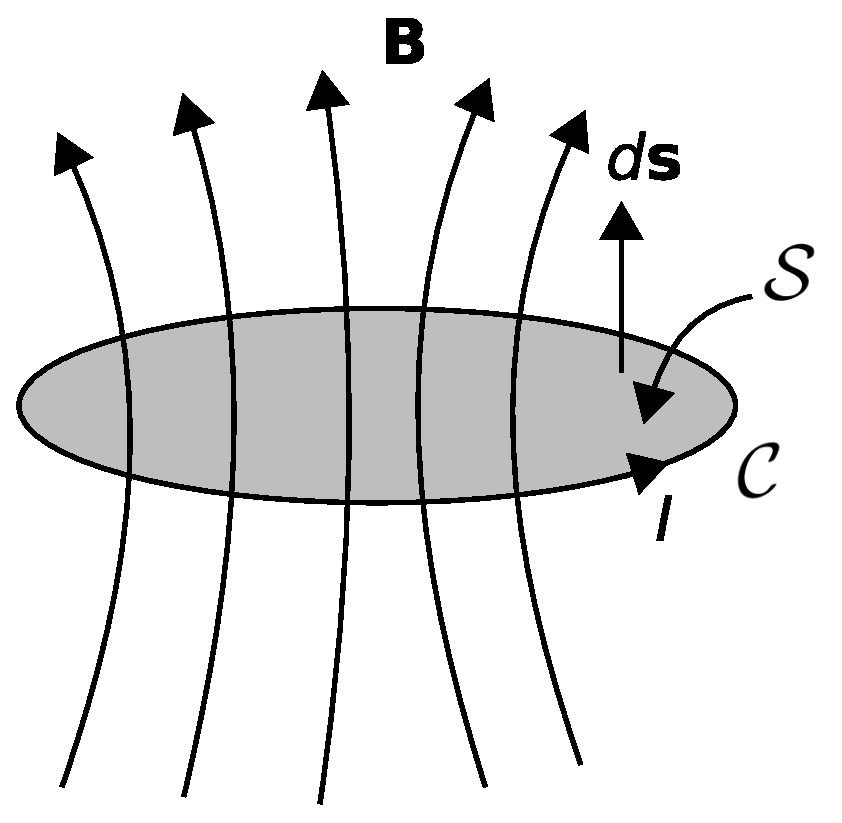
\includegraphics[width=2in]{modules/m0123_fFluxCurrent.eps}
% https://commons.wikimedia.org/wiki/File:M0123_fFluxCurrent.svg
}}{A circular surface, S, bounded by closed path C. On C, an arrow labeled I is pointing in a counterclockwise direction, following Stokes' Theorem. A vector labeled ds points out of the surface S. Five vectors labeled B go through the middle of S and point upward: The left three are curved to the left, and the right two are curved to the right.}
\end{center} 
\centerline{\scriptsize 
\copyright~\hyperref[m0123_fFluxCurrent_Credit]{K.\ Kikkeri} 
\href{https://creativecommons.org/licenses/by-sa/4.0/}{CC BY~SA 4.0} 
} 
\caption{
\label{m0123_fFluxCurrent}
Association between a closed loop of current and the associated magnetic flux.
}
\end{figure}

Many structures consist of multiple such loops -- the coil 
\index{coil}
is of course one of these.
In a coil, each winding carries the same current, and the magnetic fields of the windings add to create a magnetic field, which grows in proportion to the winding density (Section~\ref{m0120_Magnetic_Field_of_a_Coil}).
The magnetic flux density inside a coil is proportional to the number of windings, $N$, so 
the flux $\Phi$ in Equation~\ref{m0123_Ldef} should properly be indicated as $N\Phi$.
Another way to look at this is that we are counting the number of times the same current is able to generate a unique set of magnetic field lines that intersect ${\mathcal S}$.
%For this reason it is common to refer to the quantity $N\Phi$ as ``flux linkages''.

Summarizing, our complete definition for inductance is
%
\begin{equation}
\boxed{
L = \frac{N\Phi}{I}~~\mbox{(identical linkages)}
}
\label{m0123_Ldef2}
\end{equation} 
%
%ORB HIGHLIGHT
\begin{mdframed}[backgroundcolor=yellow!20,nobreak=true] 
An engineering definition of inductance 
\index{inductance!definition}
is Equation~\ref{m0123_Ldef2}, with the magnetic flux defined to be that associated with a single closed loop of current with sign convention as indicated in Figure~\ref{m0123_fFluxCurrent}, and $N$ defined to be the number of times the same current $I$ is able to create that flux.
\end{mdframed}
%
What happens if the loops have different shapes?  For example, what if the coil is not a cylinder, but rather cone-shaped? (Yes, there is such a thing -- see ``Additional Reading'' at the end of this section.)  In this case, one needs a better way to determine the factor $N\Phi$ since the flux associated with each loop of current will be different.  
However, this is beyond the scope of this section.  

An \emph{inductor} 
\index{inductor}
is a device that is designed to exhibit a specified inductance.
We can now make the connection to the concept of the inductor as it appears in elementary circuit theory.
First, we rewrite Equation~\ref{m0123_Ldef2} as follows:
%
\begin{equation}
I = \frac{N\Phi}{L}
\end{equation} 
%
Taking the derivative of both sides of this equation with respect to time, we obtain:
%
\begin{equation}
\frac{d}{dt}I = \frac{N}{L}\frac{d}{dt}\Phi
\label{m0123_edIdt}
\end{equation} 
%
Now we need to reach beyond the realm of magnetostatics for just a moment. 
Section~\ref{m0055_Faradays_Law} (``Faraday's Law'') shows that the change in $\Phi$ associated with a change in current %non-zero $dI/dt$ 
results in the creation of an electrical potential equal to $-Nd\Phi/dt$ realized over the loop ${\mathcal C}$.  
In other words, the terminal voltage $V$ is $+Nd\Phi/dt$, with the change of sign intended to keep the result consistent with the sign convention relating current and voltage in passive devices.
Therefore, $d\Phi/dt$ in Equation~\ref{m0123_edIdt} is equal to $V/N$.
Making the substitution we find:
%
\begin{equation}
V = L\frac{d}{dt}I
\label{m0125_eLCT} 
\end{equation}
%
This is the expected relationship from elementary circuit theory.

Another circuit theory concept related to inductance is \emph{mutual inductance}.  
\index{mutual inductance}
Whereas inductance relates changes in current to instantaneous voltage in the same device (Equation~\ref{m0125_eLCT}), mutual inductance relates changes in current in one device to instantaneous voltage in a \emph{different} device.  This can occur when the two devices are coupled (``linked'') by the same magnetic field.  For example, \emph{transformers}
\index{transformer}
(Section~\ref{m0031_Transformers_Principle_of_Operation}) typically consist of separate coils that are linked by the same magnetic field lines.  The voltage across one coil may be computed as the time-derivative of current on the other coil times the mutual inductance.   

Let us conclude this section by taking a moment to dispel a common misconception about inductance.  
The misconception pertains to the following question.  If the current does not form a closed loop, what is the inductance?
For example, engineers sometimes refer to the inductance of a pin or lead of an electronic component.
A pin or lead is not a closed loop, so the formal definition of inductance given above -- ratio of magnetic flux to current -- does not apply.
The broader definition of inductance -- the ability to store energy in a magnetic field -- does apply, but this is \emph{not} what is meant by ``pin inductance'' or ``lead inductance.''  
What is actually meant is the imaginary part of the impedance of the pin or lead -- i.e., the reactance -- expressed as an equivalent inductance.
In other words, the reactance of an inductive device is positive, so any device that also exhibits a positive reactance can be viewed from a circuit theory perspective as an equivalent inductance.  
This is not referring to the storage of energy in a magnetic field; it merely means that the device can be modeled as an inductor in a circuit diagram.
In the case of ``pin inductance,'' the culprit is not actually inductance, but rather skin effect 
\index{skin effect}
(see ``Additional References'' at the end of this section).
Summarizing: 
%
%ORB HIGHLIGHT
\begin{mdframed}[backgroundcolor=yellow!20,nobreak=true] 
Inductance implies positive reactance, but positive reactance 
\index{reactance}
does not imply the physical mechanism of inductance. 
\end{mdframed}

%------------------------------------
 
{\bf Additional Reading:}
\begin{itemize}
\item ``\href{https://en.wikipedia.org/wiki/Inductance}{Inductance}'' on Wikipedia.
\item ``\href{https://en.wikipedia.org/wiki/Inductor}{Inductor}'' on Wikipedia.
\item T.A.\ Winslow, ``\href{https://doi.org/10.1109/MMW.2005.1418000}{Conical Inductors for Broadband Applications},'' \emph{IEEE Microwave Mag.}, Vol.~6, No.~1, Mar 2005, pp.~68--72.
\item ``\href{https://en.wikipedia.org/wiki/Skin_effect}{Skin Effect}'' on Wikipedia.
\end{itemize}

\index{inductance|)}

      \vfill\break
    \section{Inductance of a Straight Coil}
{\color{blue}\tiny[m0124]}      % This is text associated with the open textbook "Open Electromagnetics"
% See immediately below for author, date
% This work is licensed under the Creative Commons Attribution-ShareAlike 4.0 International License. (CC BY SA 4.0) 
% To view a copy of the license, visit http://creativecommons.org/licenses/by-sa/4.0/

%ORB TITLE Inductance of a Straight Coil
%ORB AUTHOR 0        # S.W. Ellingson, Virginia Tech (ellingson@vt.edu)
%ORB DATE 20180804   # yyyymmdd
%ORB ABSTRACT Inductance of a Straight Coil

\label{m0124_Inductance_of_a_Straight_Coil} % <-- Must match name of this file and module directory name.  Don't mess with this!
\index{inductor!straight coil|(}

In this section, we determine the inductance of a straight coil, 
\index{coil}
as shown in Figure~\ref{m0124_fCoil}.
The coil is circular with radius $a$ and length $l$ and consists of $N$ windings of wire wound with uniform winding density.
Also, we assume the winding density $N/l$ is large enough that magnetic field lines cannot enter or exit between windings but rather must traverse the entire length of the coil.
Since the coil forms a cylinder, the problem is easiest to work in cylindrical coordinates with the axis of the coil aligned along the $z$ axis.
%
\begin{figure}[b!]
\begin{center}
\pdftooltip{{  % note double braces
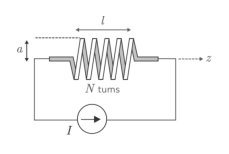
\includegraphics[width=2.5in]{modules/m0124_fCoil.eps}
}}{A circular coil with radius a and length l, consisting of N turns wound uniformly lies on the z-axis in a series circuit with current pointed to the right running counterclockwise.}
\end{center} 
% ***WikipediaCommonsURL
%\centerline{\scriptsize 
%\copyright~\hyperref[m0124_fCoil_Credit]{author} 
%\href{https://creativecommons.org/licenses/by-sa/4.0/}{CC BY~SA 4.0} 
%}
\caption{
\label{m0124_fCoil}
Determination of the inductance of a straight coil.
}
\end{figure}  

Inductance $L$ in this case is given by (Section~\ref{m0123_Inductance})
%
\begin{equation}
L = \frac{N\Phi}{I}
\label{m0124_eLdef}
\end{equation} 
%
where $I$ is current and $\Phi$ is the magnetic flux associated with one winding of the coil.  Magnetic flux in this case is given by
%
\begin{equation}
\Phi = \int_{\mathcal S}{\bf B}\cdot d{\bf s}
\end{equation}
%
where ${\bf B}$ is the magnetic flux density (units of T = Wb/m$^2$), ${\mathcal S}$ is the surface bounded by a single current loop, and $d{\bf s}$ points in the direction determined by the right hand rule with respect to the direction of positive current flow.

First, let's determine the magnetic field.
The magnetic flux density deep inside the coil is (Section~\ref{m0120_Magnetic_Field_of_a_Coil}):
%
\begin{equation}
{\bf B} \approx \hat{\bf z}\frac{\mu NI}{l} 
\label{m0124_eBapprox}
\end{equation}
%
Is it reasonable to use this approximation here?  
Since inductance pertains to energy storage, the question is really what fraction of the energy is stored in a field that is well-described by this approximation, as opposed to energy stored in the ``fringing field'' 
\index{fringing (field)}
close to the ends of the coil.  If we make $l$ sufficiently large relative to $a$, then presumably energy storage in the fringing field will be negligible in comparison.  Since the alternative leads to a much more complicated problem, we shall assume that Equation~\ref{m0124_eBapprox} is valid for the interior of the coil.

Next, we determine $\Phi$.
In this case, a natural choice for ${\mathcal S}$ is the interior cross-section of the coil in a plane perpendicular to the axis.
The direction of $d{\bf s}$ must be $+\hat{\bf z}$ since this is the direction in which the fingers of the right hand point when the current flows in the direction indicated in Figure~\ref{m0124_fCoil}.
Thus, we have
%
\begin{flalign}
\Phi &\approx \int_{\mathcal S}\left(\hat{\bf z}\frac{\mu NI}{l}\right)\cdot \left(\hat{\bf z}ds\right) \nonumber \\
~~ &= \frac{\mu NI}{l} \int_{\mathcal S}ds \nonumber \\
~~ &= \frac{\mu NI}{l}A 
\end{flalign} 
%
where $A$ is the cross-sectional area of the coil. 

Finally from Equation~\ref{m0124_eLdef} we obtain
%
\begin{equation}
\boxed{
L \approx \frac{\mu N^2 A}{l} ~~(l\gg a)
}
\label{m0124_eLlsc}
\end{equation} 
%
Note that this is dimensionally correct; that is, permeability (units of H/m) times area (units of m$^2$) divided by length (units of m) gives units of H, as expected.
Also, it is worth noting that inductance is proportional to permeability and cross-sectional area, and inversely proportional to length.
Interestingly the inductance is proportional to $N^2$ as opposed to $N$; this is because field strength increases with $N$, and independently there are $N$ flux linkages.
Finally, we note that the inductance does not depend on the \emph{shape} of the coil cross-section, but only on the \emph{area} of the cross-section.
Summarizing:
%
%ORB HIGHLIGHT
\begin{mdframed}[backgroundcolor=yellow!20,nobreak=true] 
The inductance of a long straight coil is given approximately by Equation~\ref{m0124_eLlsc}. 
\end{mdframed}

Again, this result is approximate because it neglects the non-uniform fringing field near the ends of the coil and the possibility that magnetic field lines escape between windings due to inadequate winding density.
Nevertheless, this result facilitates useful engineering analysis and design.

%------------------------------------

{\bf Additional Reading:}
\begin{itemize}
\item ``\href{https://en.wikipedia.org/wiki/Inductance}{Inductance}'' on Wikipedia.
\end{itemize}

\index{inductor!straight coil|)}

      \vfill\break
    \section{Inductance of a Coaxial Structure}
{\color{blue}\tiny[m0125]}      % This is text associated with the open textbook "Open Electromagnetics"
% See immediately below for author, date
% This work is licensed under the Creative Commons Attribution-ShareAlike 4.0 International License. (CC BY SA 4.0) 
% To view a copy of the license, visit http://creativecommons.org/licenses/by-sa/4.0/

%ORB TITLE Inductance of a Coaxial Structure
%ORB AUTHOR 0        # S.W. Ellingson, Virginia Tech (ellingson@vt.edu)
%ORB DATE 20180806   # yyyymmdd
%ORB ABSTRACT Inductance of a Coaxial Transmission Line

\label{m0125_Inductance_of_a_Coaxial_Transmission_Line} % <-- Must match name of this file and module directory name.  Don't mess with this!
\index{inductor!coaxial|(}

Let us now determine the inductance of coaxial structure, shown in Figure~\ref{m0125_fIndCoax}.
The inductance of this structure is of interest for a number of reasons -- in particular, for determining the characteristic impedance of coaxial transmission line, as addressed in Section~\ref{m0143_Coaxial_Line}.

For our present purpose, we may model the structure as shown in Figure~\ref{m0125_fIndCoax}.
This model consists of two concentric perfectly-conducting cylinders of radii $a$ and $b$, separated by a homogeneous material having permeability $\mu$.
To facilitate analysis, let us place the $+z$ axis along the common axis of the concentric cylinders, so that the cylinders may be described as the surfaces $\rho=a$ and $\rho=b$.
%
\begin{figure}[b!]
\begin{center}
\pdftooltip{{  % note double braces
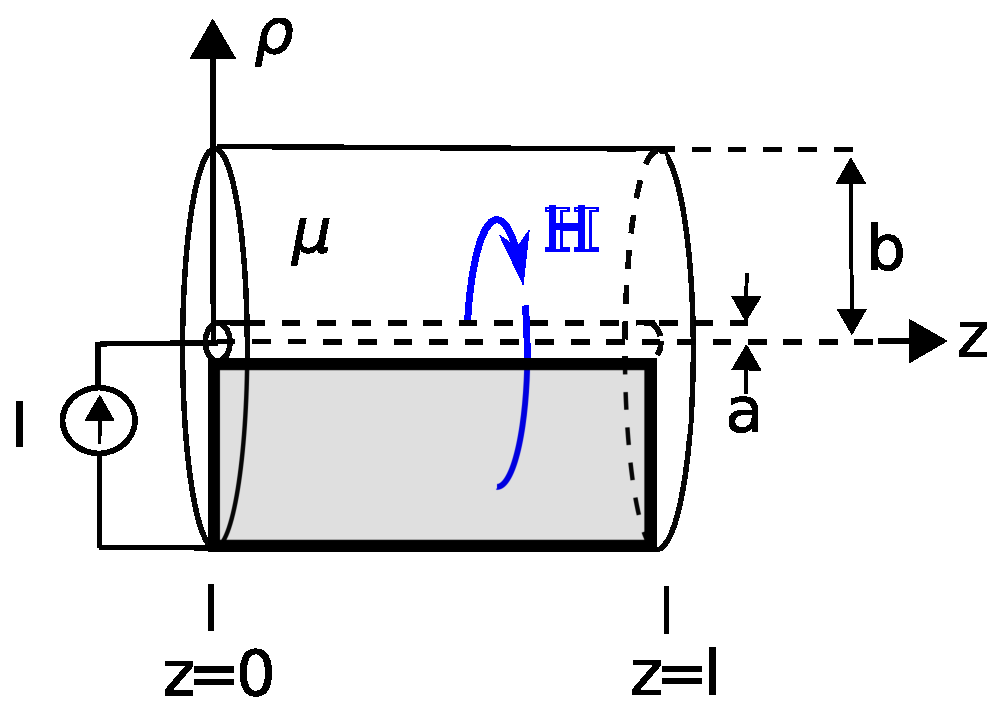
\includegraphics[width=2.5in]{modules/m0125_IndCoax.eps}
}}{Two concentric cylindrical conductors of radii a (inner) and b (outer), centered horizontally over the z-axis with length from z=0 to z=l. The permeability of the region between the cylinders is mu. A vector, rho, extends upward from the center conductor. Current is shown clockwise moving from outer to inner. Between the inner and outer conductor, is a blue 3D circle labeled H coming out of the page. The cross-section is shown as a bold, shaded rectangle. }
\end{center} 
% ***WikipediaCommonsURL
%\centerline{\scriptsize 
%\copyright~\hyperref[m0113_fCapCoax_Credit]{author} 
%\href{https://creativecommons.org/licenses/by-sa/4.0/}{CC BY~SA 4.0} 
%} 
\caption{
\label{m0125_fIndCoax}
Determining the inductance of coaxial line.
}
\end{figure}

Below we shall find the inductance by assuming a current $I$ on the inner conductor and integrating over the resulting magnetic field to obtain the magnetic flux $\Phi$ between the conductors.  Then, inductance can be determined as the ratio of the response flux to the source current.

Before we get started, note the derivation we are about to do is similar to the derivation of the \emph{capacitance} of a coaxial structure, addressed in Section~\ref{m0113_Capacitance_of_Coaxial_Line}.  The reader may benefit from a review of that section before attempting this derivation.

The first step is to find the magnetic field inside the structure.
This is relatively simple if we may neglect fringing fields, 
\index{fringing (field)}
since then the internal field may be assumed to be constant with respect to $z$.
This analysis will also apply to the case where the length $l$ pertains to one short section of a much longer structure; in this case we will obtain the inductance \emph{per length} as opposed to the total inductance for the structure.
Note that the latter is exactly what we need for the transmission line lumped-element equivalent circuit model (Section~\ref{m0029_Lumped-Element_Model}).

To determine the inductance, we invoke the definition (Section~\ref{m0123_Inductance}):
%
\begin{equation}
L \triangleq \frac{\Phi}{I}
\label{m0125_eIndDef}
\end{equation}
%
A current $I$ flowing in the $+z$ direction on the inner conductor gives rise to a magnetic field inside the coaxial structure.
The magnetic field intensity for this scenario was determined in Section~\ref{m0119_Magnetic_Field_of_a_Long_Wire} where we found
%
\begin{equation}
{\bf H} = \hat{\phi} \frac{I}{2\pi \rho} ~~, ~~ a \le\rho\le b
\end{equation}
%
The reader should note that in that section we were considering merely a line of current; not a coaxial structure.
So, on what basis do we claim the field for inside the coaxial structure is the same?
This is a consequence of Ampere's Law 
\index{Ampere's law!magnetostatics}
(Section~\ref{m0019_Amperes_Law_Magnetostatics}):
%
\begin{equation}
\oint_{\mathcal C} {\bf H}\cdot d{\bf l} = I_{encl}
\end{equation}
%
If in this new problem we specify the same circular path $\mathcal{C}$ with radius greater than $a$ and less than $b$, then the enclosed current is simply $I$.
The presence of the outer conductor does not change the radial symmetry of the problem, and nothing else remains that can change the outcome.
This is worth noting for future reference:
%
%ORB HIGHLIGHT
\begin{mdframed}[backgroundcolor=yellow!20,nobreak=true] 
The magnetic field inside a coaxial structure comprised of concentric conductors bearing current $I$ is identical to the magnetic field of the line current $I$ in free space.
\end{mdframed}

We're going to need magnetic flux density (${\bf B}$) as opposed to ${\bf H}$ in order to get the magnetic flux.
This is simple since they are related by the permeability of the medium; i.e., ${\bf B}=\mu{\bf H}$.
Thus:
%
\begin{equation}
{\bf B} = \hat{\phi} \frac{\mu I}{2\pi \rho} ~~, ~~ a \le\rho\le b
\end{equation}

Next, we get $\Phi$ by integrating over the magnetic flux density
%
\begin{equation}
\Phi = \int_{\mathcal S}{ {\bf B} \cdot d{\bf s} }
\end{equation}
%
where $\mathcal{S}$ is any open surface through which all magnetic field lines within the structure must pass.
Since this can be \emph{any} such surface, we may as well choose the simplest one.
The simplest such surface is a plane of constant $\phi$, since such a plane is a constant-coordinate surface and perpendicular to the magnetic field lines.
This surface is shown as the shaded area in Figure~\ref{m0125_fIndCoax}.
Using this surface we find:
%
\begin{flalign}
\Phi &= \int_{\rho=a}^b \int_{z=0}^l { \left( \hat{\bf \phi} \frac{\mu I}{2\pi\rho} \right) \cdot \left(\hat{\bf \phi}~d\rho~dz\right) }  \nonumber \\
%  &=  \frac{\mu I}{2\pi} \int_{\rho=a}^b \int_{z=0}^l { \frac{d\rho}{\rho} dz }  \nonumber \\
  &=  \frac{\mu I}{2\pi} \left( \int_{z=0}^l { dz } \right)  \left( \int_{\rho=a}^b { \frac{d\rho}{\rho} } \right)  \nonumber \\
  &=  \frac{\mu I l}{2\pi} \ln\left(\frac{b}{a}\right)
\end{flalign} 

Wrapping up:
%
\begin{equation}
L \triangleq \frac{\Phi}{I} = \frac{\left(\mu Il/2\pi\right)\ln\left(b/a\right) }{ I }
\end{equation}
% 
Note that factors of $I$ in the numerator and denominator cancel out, leaving:
%
\begin{equation}
\boxed{
L = \frac{\mu l}{2\pi} \ln\left(\frac{b}{a}\right)   
}
\end{equation}
%
Note that this is dimensionally correct, having units of H. 
Also note that this is expression depends only on materials (through $\mu$) and geometry (through $l$, $a$, and $b$).
Notably, it does \emph{not} depend on current, which would imply non-linear behavior.

To make the connection back to lumped-element transmission line model parameters (Sections~\ref{m0029_Lumped-Element_Model} and \ref{m0143_Coaxial_Line}), we simply divide by $l$ to get the per-unit length parameter:
%
\begin{equation}
\boxed{
L' = \frac{\mu}{2\pi} \ln\left(\frac{b}{a}\right)   
}
\label{m0125_eLp}
\end{equation}
%
which has the expected units of H/m.

%--------------------------------

%ORB EXAMPLE
~\\ \begin{example} 
\begin{mdframed}[backgroundcolor=brown!20,linecolor=brown!20]\raggedright
Inductance of RG-59 coaxial cable.
\\~\\
RG-59 coaxial cable consists of an inner conductor having radius $0.292$~mm, an outer conductor having radius $1.855$~mm, and polyethylene (a non-magnetic dielectric) spacing material.
Estimate the inductance per length of RG-59.

{\bf Solution.}  From the problem statement, 
$a=0.292$~mm, 
$b=1.855$~mm, 
and $\mu \cong \mu_0$ since the spacing material is non-magnetic.
Using Equation~\ref{m0125_eLp}, we find $L'\cong 370$~nH/m.
\end{mdframed}\end{example}

\index{inductor!coaxial|)}

      \vfill\break
    \section{Magnetic Energy}
{\color{blue}\tiny[m0127]}      % This is text associated with the open textbook "Open Electromagnetics"
% See immediately below for author, date
% This work is licensed under the Creative Commons Attribution-ShareAlike 4.0 International License. (CC BY-SA 4.0) 
% To view a copy of the license, visit http://creativecommons.org/licenses/by-sa/4.0/

%ORB TITLE Magnetic Energy
%ORB AUTHOR 0        # S.W. Ellingson, Virginia Tech (ellingson@vt.edu)
%ORB DATE 20180806   # yyyymmdd
%ORB ABSTRACT Magnetic Energy

\label{m0127_Magnetic_Energy} % <-- Must match name of this file and module directory name.  Don't mess with this!
\index{energy!magnetostatic|(}

Consider a structure exhibiting inductance; i.e., one that is able to store energy in a magnetic field in response to an applied current.
This structure could be a coil, or it could be one of a variety of inductive structures that are not explicitly intended to be an inductor; for example, a coaxial transmission line.
When current is applied, the current-bearing elements of the structure exert forces on each other.
Since these elements are not normally free to move, we may interpret this force as potential energy stored in the magnetic field associated with the current (Section~\ref{m0123_Inductance}).

We now want to know how much energy is stored in this field. 
The answer to this question has relevance in several engineering applications. 
One issue is that any system that includes inductance is using some fraction of the energy delivered by the power supply to energize this inductance. 
In many electronic systems -- in power systems in particular -- inductors are periodically energized and de-energized at a regular rate.  Since power is energy per unit time, this consumes power.  Therefore, energy storage in inductors contributes to the power consumption of electrical systems.

The stored energy is most easily determined using circuit theory concepts.
First, we note that the electrical potential difference $v(t)$ (units of V) across an inductor is related to the current $i(t)$ (units of A) through the inductor as follows (Section~\ref{m0123_Inductance}):
%
\begin{equation}
v(t) = L\frac{d}{dt}i(t)
\end{equation}
%
where $L$ (units of H) is the inductance.
The instantaneous power associated with the device is
%
\begin{equation}
p(t) = v(t)i(t)
\end{equation}
%
Energy (units of J) is power (units of J/s) integrated over time. 
Let $W_m$ be the energy stored in the inductor.
At some time $t_0$ in the past, $i(t_0)=0$ and $W_m=0$.
As current is applied, $W_m$ increases monotonically.
At the present time $t$, $i(t)=I$. 
Thus, the present value of the magnetic energy is:
%
\begin{equation}
W_m = \int_{t_0}^{t_0+t} p(\tau) d\tau 
\end{equation}
%
Now evaluating this integral using the relationships established above:
%
\begin{flalign}
W_m &= \int_{t_0}^{t+t_0} v(\tau) i(\tau) d\tau \nonumber \\
    &= \int_{t_0}^{t+t_0} \left[ L\frac{d}{d\tau}i(\tau) \right] i(\tau) d\tau \nonumber \\
    &= L \int_{t_0}^{t+t_0} \left[\frac{d}{d\tau}i(\tau)\right] i(\tau) d\tau 
\end{flalign}
%
Changing the variable of integration from $\tau$ (and $d\tau$) to $i$ (and $di$) we have
%
\begin{flalign}
W_m &= L \int_{t_0}^{t+t_0} \frac{di}{d\tau}~i~d\tau \nonumber \\
    &= L \int_{0}^{I} i~di
\end{flalign}
%
Evaluating the integral we obtain the desired expression
%
\begin{equation}
\boxed{
W_m = \frac{1}{2}LI^2 
}
\label{m0127_eWm}
\end{equation}
%
%ORB HIGHLIGHT
\begin{mdframed}[backgroundcolor=yellow!20,nobreak=true] 
The energy stored in an inductor in response to a steady current $I$ is Equation~\ref{m0127_eWm}.
This energy increases in proportion to inductance and in proportion to the square of current.
\end{mdframed}

The long straight coil (Section~\ref{m0124_Inductance_of_a_Straight_Coil}) is representative of a large number of practical applications, so it is useful to interpret the above findings in terms of this structure in particular.
For this structure we found
%
\begin{equation}
L = \frac{\mu N^2 A}{l} 
\end{equation} 
%
where $\mu$ is the permeability, $N$ is the number of windings, $A$ is cross-sectional area, and $l$ is length.
The magnetic field intensity inside this structure is related to $I$ by (Section~\ref{m0120_Magnetic_Field_of_a_Coil}):
%
\begin{equation}
H = \frac{NI}{l} 
\end{equation}
%
Substituting these expressions into Equation~\ref{m0127_eWm}, we obtain
%
\begin{flalign}
W_m &= \frac{1}{2}\left[\frac{\mu N^2 A}{l}\right]\left[\frac{Hl}{N}\right]^2 \nonumber \\
    &= \frac{1}{2}\mu H^2 Al 
\end{flalign}
%
Recall that the magnetic field inside a long coil is approximately uniform.
Therefore, the density of energy stored inside the coil is approximately uniform.
Noting that the product $Al$ is the volume inside the coil, we find that this energy density is $W_m/Al$; thus:
%
\begin{equation}
w_m = \frac{1}{2} \mu H^2 
\label{m0127_eED}
\end{equation}
%
which has the expected units of energy per unit volume (J/m$^3$).

The above expression provides an alternative method to compute the total magnetostatic energy in \emph{any} structure.
Within a mathematical volume ${\mathcal V}$, the total magnetostatic energy is simply the integral of the energy density over ${\mathcal V}$; i.e., 
%
\begin{equation}
W_m = \int_{\mathcal V} w_m~dv  
\end{equation}
%
This works even if the magnetic field and the permeability vary with position.
Substituting Equation~\ref{m0127_eED} we obtain:
%
\begin{equation}
\boxed{
W_m = \frac{1}{2} \int_{\mathcal V} \mu H^2 dv  
}
\label{m0127_eEDV}
\end{equation}
%
Summarizing:
%
%ORB HIGHLIGHT
\begin{mdframed}[backgroundcolor=yellow!20,nobreak=true] 
The energy stored by the magnetic field present within any defined volume is given by Equation~\ref{m0127_eEDV}.
\end{mdframed}
%
It's worth noting that this energy increases with the permeability of the medium, which makes sense since inductance is proportional to permeability.

Finally, we reiterate that although we arrived at this result using the example of the long straight coil, Equations~\ref{m0127_eED} and \ref{m0127_eEDV} are completely general.

\index{energy!magnetostatic|)}

      \vfill\break
    \section{Magnetic Materials}
{\color{blue}\tiny[m0058]}      % This is text associated with the open textbook "Open Electromagnetics"
% See immediately below for author, date
% This work is licensed under the Creative Commons Attribution-ShareAlike 4.0 International License. (CC BY SA 4.0) 
% To view a copy of the license, visit http://creativecommons.org/licenses/by-sa/4.0/

%ORB TITLE Magnetic Materials 
%ORB AUTHOR 0        # S.W. Ellingson, Virginia Tech (ellingson@vt.edu)
%ORB DATE 20180806   # yyyymmdd
%ORB ABSTRACT Magnetic Materials

\label{m0058_Magnetic_Materials} % <-- Must match name of this file and module directory name.  Don't mess with this!
\index{materials, magnetic|(}
\index{materials (properties)|(}

As noted in Section~\ref{m0003_Magnetic_Flux_Density}, magnetic fields arise in the presence of moving charge (i.e., current) and in the presence of certain materials.
In this section, we address these ``magnetic materials.''

A magnetic material may be defined as a substance that exhibits permeability 
\index{permeability}
$\mu$ (Section~\ref{m0009_Permeability}) that is significantly different from the permeability of free space $\mu_0$.
Since the magnetic flux density ${\bf B}$ is related to the magnetic field intensity ${\bf H}$ via ${\bf B}=\mu{\bf H}$, magnetic materials may exhibit magnetic flux density in response to a given magnetic field intensity that is significantly greater than that of other materials.  
Magnetic materials are also said to be ``magnetizable,'' meaning that the application of a magnetic field causes the material itself to become a source of the magnetic field.

Magnetic media are typically metals, semiconductors, or heterogeneous media containing such materials. An example is ferrite, 
\index{ferrite}
which consists of iron particles suspended in a ceramic.
\index{ceramic}
Magnetic media are commonly classified according to the physical mechanism responsible for their magnetizability.
These mechanisms include \emph{paramagnetism}, \emph{diamagnetism}, and \emph{ferromagnetism}.
All three of these mechanisms involve quantum mechanical processes operating at the atomic and subatomic level, and are not well-explained by classical physics.
These processes are beyond the scope of this book (but information is available via ``Additional References'' at the end of this section).
However, it is possible to identify some readily-observable differences between these categories of magnetic media.

{\bf Paramagnetic and diamagnetic materials} 
\index{paramagnetic material}
\index{diamagnetic material}
exhibit permeability that is only very slightly different than $\mu_0$ and typically by much less than 0.01\%.
These materials exhibit very weak and temporary magnetization.
The principal distinction between paramagnetic and diamagnetic media is in the persistence and orientation of induced magnetic fields.
Paramagnetic materials -- including aluminum, 
\index{aluminum}
magnesium, 
\index{magnesium}
and platinum 
\index{platinum}
-- exhibit a very weak persistent magnetic field, and the magnetic field induced in the material is aligned in the same direction as the impressed (external) magnetic field. 
Diamagnetic materials -- including copper, 
\index{copper}
gold, 
\index{gold}
and silicon
\index{silicon}
-- do not exhibit a persistent magnetic field, and the magnetic field induced in the material is (counter to intuition!) aligned in the \emph{opposite} direction as the impressed magnetic field.
The magnetization of paramagnetic and diamagnetic media is typically so weak that it is not often a consideration in engineering analysis and design.

%ORB HIGHLIGHT
\begin{mdframed}[backgroundcolor=yellow!20] 
Paramagnetic and diamagnetic media exhibit permeability only very slightly different than that of free space, with little or no magnetization.
\end{mdframed}

{\bf Ferromagnetic materials}, 
\index{ferromagnetic material}
on the other hand, exhibit permeability that can be many orders of magnitude greater than $\mu_0$. 
(See Appendix~\ref{m0136_Table_of_Permeabilities} for some example values.)
These materials can be readily and indefinitely magnetized, thus, permanent magnets are typically comprised of ferromagnetic materials.
Commonly-encountered ferromagnetic materials include iron, 
\index{iron}
nickel, 
\index{nickel}
and cobalt.
\index{cobalt} 

Ferromagnetic materials are significantly non-linear (see definition in Section~\ref{m0007_Properties_of_Materials}), exhibiting \emph{saturation} 
\index{saturation (magnetic)}
and \emph{hysteresis}.
This is illustrated in Figure~\ref{m0058_fMatSatHys}.
In this plot, the origin represents a ferromagnetic material that is unmagnetized and in a region free of an external magnetic field.
The external magnetic field is quantified in terms of ${\bf H}$, plotted along the horizontal axis.
As the external field is increased, so to is ${\bf B}$ in the material, according to the relationship ${\bf B}=\mu{\bf H}$.
Right away we see the material is non-linear, since the slope of the curve -- and hence $\mu$ -- is not constant.
%
\begin{figure}
\begin{center}
\pdftooltip{{  % note double braces
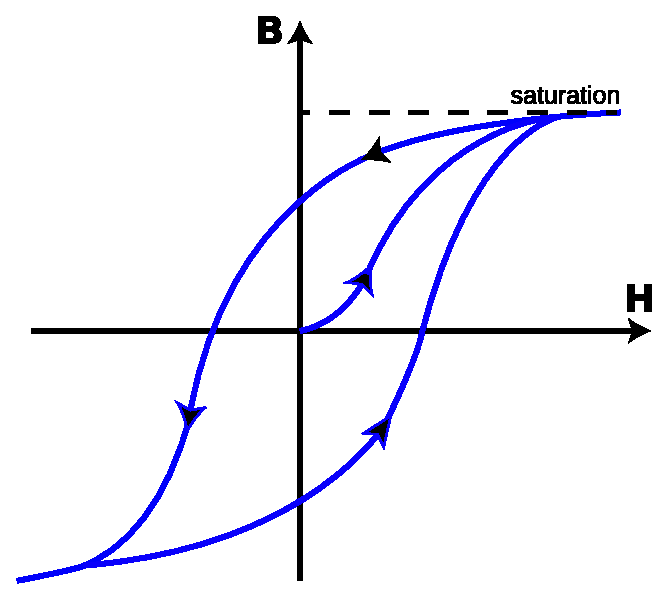
\includegraphics[width=2.5in]{modules/m0058_HysteresisSVG_se170826.eps}
% https://commons.wikimedia.org/wiki/File:HysteresisSVG.svg (modified)
}}{A two dimensional plane labeled H (vertical) - B (horizontal) plane. A blue feather like shape is shown in the plane made of 3 blue lines. At an arbitrary point on B extends a perpendicular, dashed line labeled saturation. One line is shown starting at the origin, increasing in a curve and gradually flattening at the saturation line. From that intersection point the left line increases in a negative direction through the second and third quadrants gradually flattening. The third line is a mirror image of the second line and increases from the third quadrant and gradually flattens at the saturation line.}
\end{center} 
\centerline{\scriptsize 
\copyright~\hyperref[m0058_fMatSatHys_Credit]{Ndthe} (modified)
\href{https://creativecommons.org/licenses/by-sa/3.0/deed.en}{CC BY~SA 3.0} 
} 
\caption{
\label{m0058_fMatSatHys}
Non-linearity in a ferromagnetic material manifesting as saturation and hysteresis.
}
\end{figure}

Once the external magnetizing field ${\bf H}$ exceeds a certain value, the response field ${\bf B}$ no longer significantly increases.
This is saturation. 
Once saturated, further increases in the external field result do not significantly increase the magnetization of the material, so there is no significant increase in ${\bf B}$. 

From this state of saturation, let us now reduce the external field.
We find that the rate of decrease in ${\bf B}$ with respect to ${\bf H}$ is significantly less than the rate that ${\bf B}$ originally increased with respect to ${\bf H}$.
In fact, ${\bf B}$ is still greater than zero even when ${\bf H}$ has been reduced to zero.
At this point, the magnetization of the material is obvious, and a device comprised of this material could be used as a magnet.

If we now apply an external field in the reverse direction, we find that we are eventually able to zero and then redirect the response field.
As we continue to decrease ${\bf H}$ (that is, increase the magnitude in the reverse direction), we once again reach saturation.

The same behavior is observed when we once again increase ${\bf H}$.  The material is eventually demagnetized, remagnetized in the opposite direction and then saturated in that direction.
At this point, it is apparent that a return to the start condition (${\bf H}={\bf B}=0$; i.e., demagnetized when there is no external field) is not possible.

Hysteresis is the name that we apply to this particular form of non-linear behavior.
Hysteresis has important implications in engineering applications.
First, as identified above, it is an important consideration in the analysis and design of magnets.
In applications where a ferromagnetic material is being used because high permeability is desired -- e.g., in inductors 
\index{inductor!hysteresis}
(Section~\ref{m0123_Inductance}) and transformers (Section~\ref{m0031_Transformers_Principle_of_Operation}) 
\index{transformer!hysteresis}
-- hysteresis complicates the design and imposes limits on the performance of the device.

\emph{Hysteresis} 
\index{hysteresis}
may also be exploited as a form of memory.
This is apparent from Figure~\ref{m0058_fMatSatHys}.
If ${\bf B}>0$, then recent values of ${\bf H}$ must have been relatively large and positive.  Similarly,
If ${\bf B}<0$, then recent values of ${\bf H}$ must have been relatively large and negative.
Furthermore, the most recent sign of ${\bf H}$ can be inferred even if the present value of ${\bf H}$ is zero.
In this sense, the material ``remembers'' the past history of its magnetization and thereby exhibits memory.
This is the enabling principle for a number of digital data storage devices, including hard drives (see ``Additional Reading'' at the end of this section).
Summarizing:
%
%ORB HIGHLIGHT
\begin{mdframed}[backgroundcolor=yellow!20,nobreak=true] 
Ferromagnetic media exhibit permeability $\mu$ that is orders of magnitude greater than that of free space and are readily magnetizable.  
These materials are also nonlinear in $\mu$, which manifests as saturation and hysteresis.
\end{mdframed}

%%%%%%%%%%%%%%%%%%%%%%%%%%%%%%%%%%%%%%%%

{\bf Additional Reading:}
\begin{itemize}
\item Section~\ref{m0136_Table_of_Permeabilities} (``Permeability of Some Common Materials'')
\item ``\href{https://en.wikipedia.org/wiki/Magnetism}{Magnetism}'' on Wikipedia.
\item ``\href{https://en.wikipedia.org/wiki/Ferrite_(magnet)}{Ferrite (magnet)}'' on Wikipedia.
\item ``\href{https://en.wikipedia.org/wiki/Paramagnetism}{Paramagnetism}'' on Wikipedia.
\item ``\href{https://en.wikipedia.org/wiki/Diamagnetism}{Diamagnetism}'' on Wikipedia.
\item ``\href{https://en.wikipedia.org/wiki/Ferromagnetism}{Ferromagnetism}'' on Wikipedia.
\item ``\href{https://en.wikipedia.org/wiki/Magnetic_hysteresis}{Magnetic hysteresis}'' on Wikipedia.
\item ``\href{https://en.wikipedia.org/wiki/Magnetic_storage}{Magnetic storage}'' on Wikipedia.
\item ``\href{https://en.wikipedia.org/wiki/Hard_disk_drive}{Hard disk drive}'' on Wikipedia.
\end{itemize}

\index{materials, magnetic|)}
\index{materials (properties)|)}

      \vfill\break
{\color{blue}\tiny[m0150]}    % This is text associated with the open textbook "Open Electromagnetics"
% See immediately below for author, date
% This work is licensed under the Creative Commons Attribution-ShareAlike 4.0 International License. (CC BY SA 4.0) 
% To view a copy of the license, visit http://creativecommons.org/licenses/by-sa/4.0/

%ORB TITLE Magnetostatics
%ORB AUTHOR 0        # S.W. Ellingson, Virginia Tech (ellingson@vt.edu)
%ORB DATE 20180701  # yyyymmdd
%ORB ABSTRACT End matter for chapter entitled "Magnetostatics"

\label{m0150_Ch_End_Matter_Magnetostatics} % <-- Must match name of this file and module directory name.  Don't mess with this!

\onecolumn
\section*{Image Credits}

\begin{itemize}

\item[Fig.] \label{m0018_fGLMBarMagnet_Credit}
  \ref{m0018_fGLMBarMagnet}:
  \copyright~Youming / K.\ Kikkeri, 
  \url{https://commons.wikimedia.org/wiki/File:M0018_fGLMBarMagnet_(2).svg},\\ 
  CC BY~SA 4.0 (\url{https://creativecommons.org/licenses/by-sa/4.0/}).

\item[Fig.] \label{m0019_fACL_Credit}
  \ref{m0019_fACL}:
  \copyright~K.\ Kikkeri, 
  \url{https://commons.wikimedia.org/wiki/File:M0019_fACL.svg},\\ 
  CC BY~SA 4.0 (\url{https://creativecommons.org/licenses/by-sa/4.0/}).

\item[Fig.] \label{m0119_fLSW_Credit}
  \ref{m0119_fLSW}:
  \copyright~K.\ Kikkeri, 
  \url{https://commons.wikimedia.org/wiki/File:M0119_fLSW.svg},\\ 
  CC BY~SA 4.0 (\url{https://creativecommons.org/licenses/by-sa/4.0/}).

\item[Fig.] \label{m0119_fRightHandRule_Credit}
  \ref{m0119_fRightHandRule}:
  \copyright~Jfmelero, 
  \url{https://et.wikipedia.org/wiki/Fail:Manoderecha.svg},\\ 
  CC BY~SA 4.0 (\url{https://creativecommons.org/licenses/by-sa/4.0/}),
  modified.
  %Modified as follows: ``${\bf B}$'' replaced with ``${\bf H}$''.

\item[Fig.] \label{m0120_fStraightCoil_Credit}
  \ref{m0120_fStraightCoil}:
  Zureks,  
  \url{https://en.wikipedia.org/wiki/File:Solenoid-1.png},\\ 
  public domain.

\item[Fig.] \label{m0120_fStraightCoilFieldLines_Credit}
  \ref{m0120_fStraightCoilFieldLines}:
  \copyright~Geek3, 
  \url{https://commons.wikimedia.org/wiki/File:VFPt_Solenoid_correct.svg},\\ 
  CC BY~SA 3.0 (\url{https://creativecommons.org/licenses/by-sa/3.0/}).

\item[Fig.] \label{m0120_fOneTurn_Credit}
  \ref{m0120_fOneTurn}:
  Chetvorno,  
  \url{https://en.wikipedia.org/wiki/File:Magnetic_field_of_loop_3.svg},\\ 
  public domain via \href{https://creativecommons.org/publicdomain/zero/1.0/deed.en}{CC0 1.0},
  modified.

\item[Fig.] \label{m0120_fPath_Credit}
  \ref{m0120_fPath}:
  \copyright~K.\ Kikkeri, 
  \url{https://commons.wikimedia.org/wiki/File:M0120_fPath.svg},\\ 
  CC BY~SA 4.0 (\url{https://creativecommons.org/licenses/by-sa/4.0/}).

\item[Fig.] \label{m0049_fToroidalCoilExample_Credit}
  \ref{m0049_fToroidalCoilExample}:
  Slick, 
  https://en.wikipedia.org/wiki/File:\\ 
     3Com\_OfficeConnect\_ADSL\_Wireless\_11g\_Firewall\_Router\_2012-10-28-0869.jpg,\\ 
  % https://en.wikipedia.org/wiki/File:3Com_OfficeConnect_ADSL_Wireless_11g_Firewall_Router_2012-10-28-0869.jpg
  public domain via CC0 1.0 (\url{https://creativecommons.org/publicdomain/zero/1.0/deed.en}).

\item[Fig.] \label{m0022_fBoundary_Credit}
  \ref{m0022_fBoundary}:
  \copyright~K.\ Kikkeri, 
  \url{https://commons.wikimedia.org/wiki/File:M0022_fBoundary.svg},\\ 
  CC BY~SA 4.0 (\url{https://creativecommons.org/licenses/by-sa/4.0/}).

\item[Fig.] \label{m0123_fFluxCurrent_Credit}
  \ref{m0123_fFluxCurrent}:
  \copyright~K.\ Kikkeri, 
  \url{https://commons.wikimedia.org/wiki/File:M0123_fFluxCurrent.svg},\\ 
  CC BY~SA 4.0 (\url{https://creativecommons.org/licenses/by-sa/4.0/}).

\item[Fig.] \label{m0058_fMatSatHys_Credit}
  \ref{m0058_fMatSatHys}:
  \copyright~Ndthe, 
  \url{https://commons.wikimedia.org/wiki/File:HysteresisSVG.svg},\\ 
  CC BY~SA 3.0 (\url{https://creativecommons.org/licenses/by-sa/3.0/deed.en}), 
  modified by author.

\end{itemize}

\twocolumn

  \chapter{Time-Varying Fields}
  \thispagestyle{fancy} % override footer in first page of chapter
  \fancyhf{}            % reset header and footer
  \fancyfoot[C]{\footnotesize \emph{Electromagnetics Vol~1}. ~\copyright~2018 S.W.\ Ellingson ~CC~BY~SA~4.0. ~\url{https://doi.org/10.21061/electromagnetics-vol-1}}
    \section{Comparison of Static and Time-Varying Electromagnetics}
{\color{blue}\tiny[m0013]}      % This is text associated with the open textbook "Open Electromagnetics"
% See immediately below for author, date
% This work is licensed under the Creative Commons Attribution-ShareAlike 4.0 International License. (CC BY-SA 4.0) 
% To view a copy of the license, visit http://creativecommons.org/licenses/by-sa/4.0/

%ORB TITLE Comparison of Static and Time-Varying Electromagnetics 
%ORB AUTHOR 0        # S.W. Ellingson, Virginia Tech (ellingson@vt.edu)
%ORB DATE 20180807   # yyyymmdd
%ORB ABSTRACT Comparison of Static and Time-Varying Electromagnetics 

\label{m0013_Comparison_of_Static_and_Time-Varying_Electromagnetics} % <-- Must match name of this file and module directory name.  Don't mess with this!

Students encountering time-varying electromagnetic fields for the first time have usually been exposed to electrostatics and magnetostatics already.
These disciplines exhibit many similarities as summarized in Table~\ref{m0013_tComparison}.
The principles of time-varying electromagnetics presented in this table are all formally introduced in other sections; the sole purpose of this table is to point out the differences. 
We can summarize the differences as follows:
%
%ORB HIGHLIGHT
\begin{mdframed}[backgroundcolor=yellow!20,nobreak=true] 
Maxwell's Equations in the general (time-varying) case include extra terms that do not appear in the equations describing electrostatics and magnetostatics.
These terms involve time derivatives of fields and describe coupling between electric and magnetic fields.
\end{mdframed}  
%
%\onecolumn
\begin{table*}[t]
\begin{center}
\begin{tabular}{lll}
~ & {\bf Electrostatics /} & {\bf Time-Varying} \\
~ & {\bf Magnetostatics}   & {\bf (Dynamic)} \\
\hline\hline
Electric \& magnetic & independent  & {\color{blue}possibly coupled} \\
fields are...       & ~  & ~ \\
\hline
Maxwell's Eqns. & $\oint_{\mathcal S}{{\bf D}\cdot d{\bf s}} = Q_{encl}$  & $\oint_{\mathcal S}{{\bf D}\cdot d{\bf s}} = Q_{encl}$ \\
~~(integral)   & $\oint_{\mathcal C}{{\bf E}\cdot d{\bf l}} = 0$         & $\oint_{\mathcal C}{{\bf E}\cdot d{\bf l}} = {\color{blue}-\frac{\partial}{\partial t}\int_{\mathcal S}{\bf B}\cdot d{\bf s}}$ \\
               & $\oint_{\mathcal S}{{\bf B}\cdot d{\bf s}} = 0$         & $\oint_{\mathcal S}{{\bf B}\cdot d{\bf s}} = 0$ \\
               & $\oint_{\mathcal C}{{\bf H}\cdot d{\bf s}} = I_{encl}$  & $\oint_{\mathcal C}{{\bf H}\cdot d{\bf l}} = I_{encl} {\color{blue} + \int_{\mathcal S}\frac{\partial}{\partial t}{\bf D}\cdot d{\bf s}}$ \\
\hline
Maxwell's Eqns.     & $\nabla\cdot{\bf D}=\rho_v$   & $\nabla\cdot{\bf D}=\rho_v$ \\
~~(differential)   & $\nabla\times{\bf E}=0$       & $\nabla\times{\bf E}={\color{blue}-\frac{\partial}{\partial t}{\bf B}}$ \\
                   & $\nabla\cdot{\bf B}=0$        & $\nabla\cdot{\bf B}=0$ \\
                   & $\nabla\times{\bf H}={\bf J}$ & $\nabla\times{\bf H}={\bf J} {\color{blue}+ \frac{\partial}{\partial t}{\bf D}}$ \\
\hline
\end{tabular}
\end{center}
\label{m0013_tComparison}
\caption{Comparison of principles governing static and time-varying electromagnetic fields.  Differences in the time-varying case relative to the static case are highlighted in {\color{blue}blue}.
\index{Maxwell's equations} 
}
\end{table*}
%\twocolumn

The coupling between electric and magnetic fields in the time-varying case has one profound consequence in particular. 
It becomes possible for fields to continue to exist even after their sources -- i.e., charges and currents -- are turned off.  
What kind of field can continue to exist in the absence of a source?  
Such a field is commonly called a \emph{wave}.
Examples of waves include signals in transmission lines and signals propagating away from an antenna. 


%-------------------------------------------------------

{\bf Additional Reading:}
\begin{itemize}
\item ``\href{https://en.wikipedia.org/wiki/Maxwell's_equations}{Maxwell's Equations}'' on Wikipedia.
\end{itemize}

      \vfill\break
    \section{Electromagnetic Induction}
{\color{blue}\tiny[m0129]}      % This is text associated with the open textbook "Open Electromagnetics"
% See immediately below for author, date
% This work is licensed under the Creative Commons Attribution-ShareAlike 4.0 International License. (CC BY-SA 4.0) 
% To view a copy of the license, visit http://creativecommons.org/licenses/by-sa/4.0/

%ORB TITLE Electromagnetic Induction
%ORB AUTHOR 0        # S.W. Ellingson, Virginia Tech (ellingson@vt.edu)
%ORB DATE 20180807   # yyyymmdd
%ORB ABSTRACT Electromagnetic induction and Lenzs' Law

\label{m0129_Electromagnetic_Induction} % <-- Must match name of this file and module directory name.  Don't mess with this!
\index{induction|(}

When an electrically-conducting structure is exposed to a time-varying magnetic field, an electrical potential difference is induced across the structure.
This phenomenon is known as \emph{electromagnetic induction}. 
A convenient introduction to electromagnetic induction is provided by Lenz's Law.
\index{Lenz's law}
This section explains electromagnetic induction in the context of Lenz's Law and provides two examples.

Let us begin with the example depicted in
Figure~\ref{m0129_fLenzLaw}, involving a cylindrical coil.  
Attached to the terminals of the coil is a resistor for which we may identify an electric potential difference $V$ and current $I$.
In this particular case, the sign conventions indicated for $V$ and $I$ are arbitrary, but it is important to be consistent once they are established.
%
\begin{figure}
\begin{center}
\pdftooltip{{  % note double braces
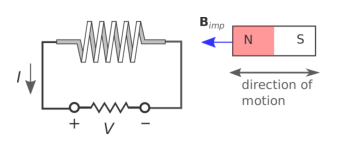
\includegraphics[width=\columnwidth]{modules/m0129_fLenzLaw.eps}
% URL
}}{A circular coil consisting of N turns wound uniformly lies in a rectangular series circuit with a resistor, V, between positive and negative nodes. The current is moving from the coil in a counterclockwise direction. To the right of the coil is a horizontal bar magnet, with the north side pointing toward the coil. A blue vector extends from the magnet toward the coil, labeled B sub imp. Under the magnet is a horizontal double headed arrow, labeled "direction of motion".}
\end{center} 
\centerline{\scriptsize 
\hyperref[m0129_fLenzLaw_credit]{Y.\ Qin} (modified) 
\href{https://creativecommons.org/licenses/by/4.0/}{CC BY 4.0} 
} 
\caption{
\label{m0129_fLenzLaw}
An experiment demonstrating electromagnetic induction and Lenz's Law.
}
\end{figure}

Now let us introduce a bar magnet as shown in Figure~\ref{m0129_fLenzLaw}.
The magnet is centered along the axis of coil, to the right of the coil, and with its north pole facing toward the coil.
The magnet is responsible for the magnetic flux density ${\bf B}_{imp}$.
We refer to ${\bf B}_{imp}$ as an \emph{impressed} magnetic field because this field exists independently of any response that may be induced by interaction with the coil.
Note that ${\bf B}_{imp}$ points to the left inside the coil.

The experiment consists of three tests.
We will find in two of these tests that current flows (i.e., $\left|I\right|>0$), and subsequently, there is an \emph{induced} magnetic field ${\bf B}_{ind}$ due to this current.
It is the direction of the current and subsequently the direction of ${\bf B}_{ind}$ inside the coil that we wish to observe.
The findings are summarized below and in Table~\ref{m0129_tLenzLaw}.
%
\begin{itemize}
\item When the magnet is motionless, we have the unsurprising result that there is no current in the coil. Therefore, no magnetic field is induced, and the total magnetic field is simply equal to ${\bf B}_{imp}$.
\item When the magnet moves \emph{toward} the coil, we observe current that is positive with respect to the reference direction indicated in Figure~\ref{m0129_fLenzLaw}.  This current creates an induced magnetic field ${\bf B}_{ind}$ that points to the \emph{right}, as predicted by magnetostatic considerations from the right-hand rule. Since ${\bf B}_{imp}$ points to the left, it appears that the induced current is opposing the increase in the magnitude of the total magnetic field. 
\item When the magnet moves \emph{away} from the coil, we observe current that is negative with respect to the reference direction indicated in Figure~\ref{m0129_fLenzLaw}.  This current yields ${\bf B}_{ind}$ that points to the \emph{left}. Since ${\bf B}_{imp}$ points to the left, it appears that the induced current is opposing the decrease in the magnitude of the total magnetic field.
\end{itemize}
%
\begin{table*}
\begin{center}
\begin{tabular}{llll}
Magnet is ... & $\left|{\bf B}_{imp}\right|$ in coil is ... & Circuit Response & ${\bf B}_{ind}$ inside coil \\
\hline
Motionless & constant & $V=0$, $I=0$ & none \\
Moving toward coil & increasing & $V>0$, $I>0$ & Pointing right \\
Moving away from coil & decreasing & $V<0$, $I<0$ & Pointing left \\
\end{tabular}
\end{center}
\caption{\label{m0129_tLenzLaw}Results of the experiment associated with Figure~\ref{m0129_fLenzLaw}.}
\end{table*}

The first conclusion one may draw from this experiment is that changes in the magnetic field can induce current.  
This was the claim made in the first paragraph of this section and is a consequence of Faraday's Law, 
\index{Faraday's law}
which is tackled in detail in Section~\ref{m0055_Faradays_Law}.
The second conclusion -- also associated with Faraday's Law -- is the point of this section:  The induced magnetic field -- that is, the one due to the current induced in the coil -- always opposes the change in the impressed magnetic field.  Generalizing:
%
%ORB HIGHLIGHT
\begin{mdframed}[backgroundcolor=yellow!20] 
Lenz's Law states that the current that is induced by a change in an impressed magnetic field creates an induced magnetic field that opposes (acts to reduce the effect of) the change in the total magnetic field.
\end{mdframed}

When the magnet moves, three things happen: (1) A current is induced, (2) A magnetic field is induced (which adds to the impressed magnetic field), and (3) the value of $V$ becomes non-zero.
Lenz's Law does not address which of these are responding directly to the change in the impressed magnetic field, and which of these are simply responding to changes in the other quantities.
Lenz's Law may leave you with the incorrect impression that it is $I$ that is induced, and that ${\bf B}_{ind}$ and $V$ are simply responding to this current.
In truth, the quantity that is induced is actually $V$.  
This can be verified in the above experiment by replacing the resistor with a high-impedance voltmeter, which will indicate that $V$ is changing even though there is negligible current flow.
Current flow is simply a response to the induced potential.
Nevertheless, it is common to say informally that ``$I$ is induced,'' even if it is only indirectly through $V$. 

So, if Lenz's Law is simply an observation and not an explanation of the underlying physics, then what is it good for?
Lenz's Law is often useful for quickly determining the direction of current flow in practical electromagnetic induction problems, without resorting to the mathematics associated with Faraday's Law.
Here's an example:

%%%%%%%%%%%%%%%%%%%%%%%%%%%%%%%%%%%%%%%%%%%%%%%
%ORB EXAMPLE
~\\ \begin{example} 
\begin{mdframed}[backgroundcolor=brown!20,linecolor=brown!20]\raggedright
Electromagnetic induction through a transformer.
\index{transformer!induction}
\\~\\
Figure~\ref{m0129_fLLCoil} shows a rudimentary circuit consisting of a battery and a switch on the left, a voltmeter on the right, and a transformer linking the two.
It is not necessary to be familiar with transformers to follow this example; suffice it to say, the transformer considered here consists of two coils wound around a common toroidal core, which serves to contain magnetic flux.  In this way, the flux generated by either coil is delivered to the other coil with negligible loss.

The experiment begins with the switch on the left in the open state.  
Thus, there is no current and no magnetic field apparent in the coil on the left.
The voltmeter reads 0~V.
When the switch is closed, what happens?

{\bf Solution.}  Closing the switch creates a current in the coil on the left. 
Given the indicated polarity of the battery, this current flows counter-clockwise through the circuit on the left, with current arriving in the left coil through the bottom terminal. 
Given the indicated direction of the winding in the left coil, the impressed magnetic field ${\bf B}_{imp}$ is oriented counter-clockwise through the toroidal core. 
The coil on the right ``sees'' ${\bf B}_{imp}$ increase from zero to some larger value.
Since the voltmeter presumably has input high impedance, negligible current flows.
However, if current were able to flow, Lenz's Law dictates that it would be induced to flow in a counter-clockwise direction around the circuit on the right, since the induced magnetic field ${\bf B}_{ind}$ would then be clockwise-directed so as to oppose the increase in ${\bf B}_{imp}$.
Therefore, the potential measured at the bottom of the right coil would be higher than the potential at the top of the right coil. 
The figure indicates that the voltmeter measures the potential at its right terminal relative to its left terminal, so the needle will deflect to the right.
This deflection will be temporary, since the current provided by the battery becomes constant at a new non-zero value and ${\bf B}_{ind}$ responds only to the \emph{change} in ${\bf B}_{imp}$.  
The voltmeter reading will remain at zero for as long as the switch remains closed and the current remains steady.

%%% TODO: Make these problems
Here are some follow up exercises to test your understanding of what is going on:
(1) Now open the switch.  What happens?
(2) Repeat the original experiment, but before starting, swap the terminals on the battery.  
\end{mdframed}
%
\begin{figure}
\begin{center}
\pdftooltip{{  % note double braces
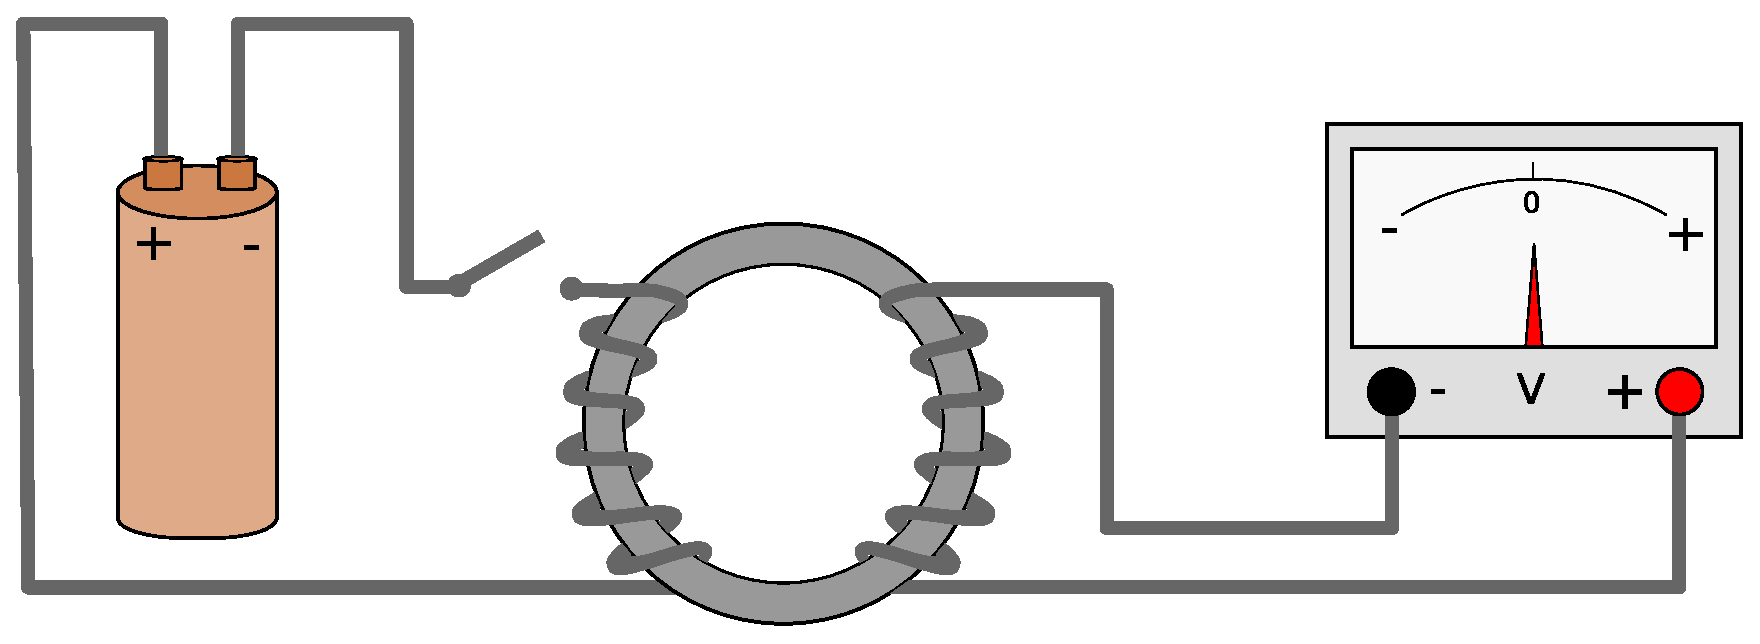
\includegraphics[width=\columnwidth]{modules/m0129_fLLCoil.eps}
% https://commons.wikimedia.org/wiki/File:Faraday_emf_experiment.svg
}}{Wire comes from the negative side of the battery and winds around one side of the loop and returns to the positive side of the battery. Wire runs around the opposite side of the loop and connects to the positive and negative leads of a voltmeter.}
\end{center} 
\centerline{\scriptsize 
\hyperref[m0129_fLLCoil_Credit]{E.\ Bach} 
\href{https://creativecommons.org/publicdomain/zero/1.0/deed.en}{CC0 1.0} (modified) 
} 
\caption{
Electromagnetic induction through a transformer.
}
\label{m0129_fLLCoil}
\end{figure}
\end{example}
%%%%%%%%%%%%%%%%%%%%%%%%%%%%%%%%%%%%%%%%%%%%%%%

Finally, it is worth noting that Lenz's law can also be deduced from the principle of conservation of energy.
The argument is that if the induced magnetic field \emph{reinforced} the change in the impressed magnetic field, then the sum magnetic field would increase.  This would result in a further increase in the induced magnetic field, leading to a positive feedback situation.  However, positive feedback cannot be supported without an external source of energy, leading to a logical contradiction.  In other words, the principle of conservation of energy requires the \emph{negative} feedback described by Lenz's law.      

{\bf Additional Reading:}
\begin{itemize}
\item ``\href{https://en.wikipedia.org/wiki/Electromagnetic_induction}{Electromagnetic Induction}'' on Wikipedia.
\item ``\href{https://en.wikipedia.org/wiki/Lenz's_law}{Lenz's Law}'' on Wikipedia.
\end{itemize}

\index{induction|)}



      \vfill\break
    \section{Faraday's Law}
{\color{blue}\tiny[m0055]}      % This is text associated with the open textbook "Open Electromagnetics"
% See immediately below for author, date
% This work is licensed under the Creative Commons Attribution-ShareAlike 4.0 International License. (CC BY-SA 4.0) 
% To view a copy of the license, visit http://creativecommons.org/licenses/by-sa/4.0/

%ORB TITLE Faraday's Law
%ORB AUTHOR 0        # S.W. Ellingson, Virginia Tech (ellingson@vt.edu)
%ORB DATE 20180807   # yyyymmdd
%ORB ABSTRACT Faraday's Law: Single-loop equation, explains procedure to get emf, explains types of emf

\label{m0055_Faradays_Law} % <-- Must match name of this file and module directory name.  Don't mess with this!
\index{Faraday's law|(}

Faraday's Law describes the generation of electric potential by a time-varying magnetic flux.
\index{flux!magnetic}
This is a form of \emph{electromagnetic induction}, 
\index{induction}
as discussed in Section~\ref{m0129_Electromagnetic_Induction}.

To begin, consider the scenario shown in Figure~\ref{m0055_fFaradaySingleLoop}. A single loop of wire in the presence of an impressed magnetic field ${\bf B}$. 
For reasons explained later, we introduce a small gap and define $V_T$ to be the potential difference measured across the gap according to the sign convention indicated.
The resistance $R$ may be any value greater than zero, including infinity; i.e., a literal gap.
%
\begin{figure}[b!]
\begin{center}
\pdftooltip{{  % note double braces
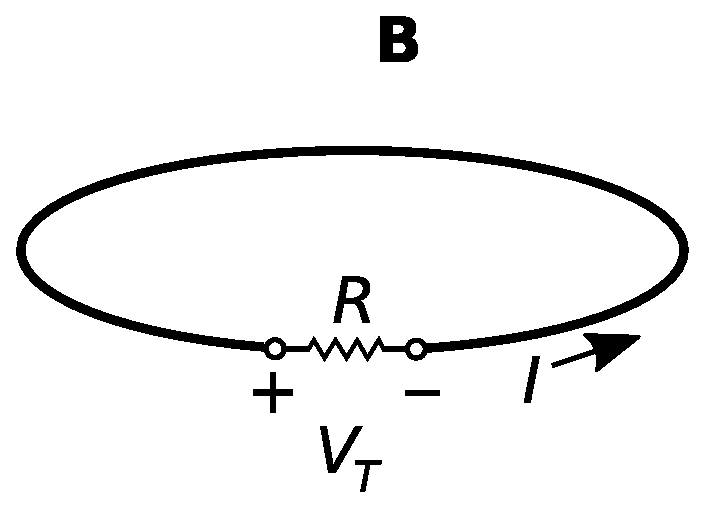
\includegraphics[width=2in]{modules/m0055_fFaradaySingleLoop.eps}
}}{A loop of wire lying in a magnetic field, B. In the loop lies a resistor, R, between a positive and negative node. Beneath the resistor is labeled V sub T. A vector, I, on the right points in a counterclockwise direction.}
\end{center} 
% ***WikipediaCommonsURL
%\centerline{\scriptsize 
%\copyright~\hyperref[***_Credit]{author} 
%\href{https://creativecommons.org/licenses/by-sa/4.0/}{CC BY-SA 4.0} 
%} 
\caption{
\label{m0055_fFaradaySingleLoop}
A single loop of wire in the presence of an impressed magnetic field.
}
\end{figure}

As long as $R$ is not infinite, we know from Lenz's Law 
\index{Lenz's law}
(Section~\ref{m0129_Electromagnetic_Induction}) to expect that a time-varying magnetic field will cause a current to flow in the wire. 
Lenz's Law also tells us the direction in which the current will flow.
However, Lenz's Law does not tell us the magnitude of the current, and it sidesteps some important physics that has profound implications for the analysis and design of electrical devices, including generators and transformers.

The more complete picture is given by Faraday's Law.
In terms of the scenario of Figure~\ref{m0055_fFaradaySingleLoop}, Faraday's Law relates the potential $V_T$ induced by the time variation of ${\bf B}$. 
$V_T$ then gives rise to the current identified in Lenz's Law. 
The magnitude of this current is simply $V_T/R$. %, oriented in the direction shown in Figure~\ref{m0055_fFaradaySingleLoop}.
Without further ado, here's Faraday's Law for this single loop scenario:
%
\begin{equation}   
V_T = - \frac{\partial}{\partial t} \Phi ~~\mbox{(single loop)}
\label{m0055_eVT}
\end{equation}
%
Here $\Phi$ is the magnetic flux (units of Wb) associated with any open surface $\mathcal{S}$ bounded by the loop:
%
\begin{equation}   
\Phi = \int_{\mathcal{S}} { {\bf B} \cdot d{\bf s} }
\label{m0055_ePhi}
\end{equation}
%
where ${\bf B}$ is magnetic flux density (units of T or Wb/m$^2$) and $d{\bf s}$ is the differential surface area vector.

To make headway with Faraday's Law, one must be clear about the meanings of $\mathcal{S}$ and $d{\bf s}$.
If the wire loop in the present scenario lies in a plane, then a good choice for $\mathcal{S}$ is the simply the planar area bounded by the loop.
However, \emph{any} surface that is bounded by the loop will work, including non-planar surfaces that extend above and/or below the plane of the loop. All that is required is that every magnetic field line that passes through the loop also passes through $\mathcal{S}$. 
This happens automatically if the curve $\mathcal{C}$ defining the edge of the open surface $\mathcal{S}$ corresponds to the loop.
Subsequently, the magnitude of $d{\bf s}$ is the differential surface element $ds$ and the direction of $d{\bf s}$ is the unit vector $\hat{\bf n}$ perpendicular to each point on $\mathcal{S}$, so $d{\bf s}=\hat{\bf n}ds$.

This leaves just one issue remaining -- the orientation of $\hat{\bf n}$.  
This is sorted out in Figure~\ref{m0055_fFaradaySingleLoopSC}.
There are two possible ways for a vector to be perpendicular to a surface, and the direction chosen for $\hat{\bf n}$ will affect the sign of $V_T$.  
Therefore, $\hat{\bf n}$ must be somehow related to the polarity chosen for $V_T$.  Let's consider this relationship.
Let $\mathcal{C}$ begin at the ``$-$'' terminal of $V_T$ and follow the entire perimeter of the loop, ending at the ``$+$'' terminal.
Then, $\hat{\bf n}$ is determined by the following ``right-hand rule:''
\index{right-hand rule!Stokes' theorem}
$\hat{\bf n}$ points in the direction of the curled fingers of the right hand when the thumb of the right hand is aligned in the direction of $\mathcal{C}$.
It's worth noting that this convention is precisely the convention used to relate $\hat{\bf n}$ and $\mathcal{C}$ in Stokes' Theorem 
\index{Stokes' theorem}
(Section~\ref{m0051_Stokes_Theorem}).
%
\begin{figure}
\begin{center}
\pdftooltip{{  % note double braces
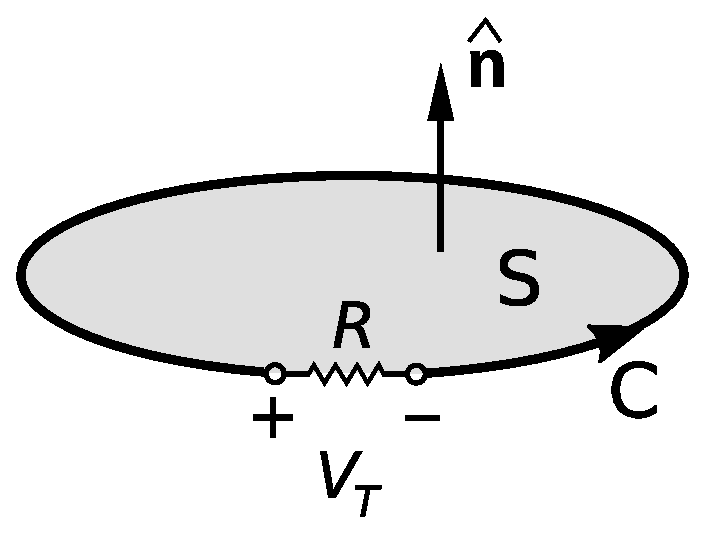
\includegraphics[width=2in]{modules/m0055_fFaradaySingleLoopSC.eps}
% ***WikipediaCommonsURL
}}{A circular surface, S, bounded by C. On C, an arrow points in a counterclockwise direction. In the loop of C lies a resistor, R, between a positive and negative node. Beneath the resistor is labeled V sub T. A vector comes out of the surface, labeled n-hat. }
\end{center} 
%\centerline{\scriptsize 
%\copyright~\hyperref[***_Credit]{author} 
%\href{https://creativecommons.org/licenses/by-sa/4.0/}{CC BY-SA 4.0} 
%} 
\caption{
\label{m0055_fFaradaySingleLoopSC}
Relationship between the polarity of $V_T$ and orientations of $\mathcal{C}$ and $\hat{\bf n}$ in the planar single-loop scenario.
}
\end{figure}

Now let us recap how Faraday's Law is applied to the single loop scenario of Figure~\ref{m0055_fFaradaySingleLoop}:
%
\begin{enumerate}
\item Assign ``$+$'' and ``$-$'' terminals to the gap voltage $V_T$.
\item The orientation of $\hat{\bf n}$ is determined by the right hand rule, taking the direction of $\mathcal{C}$ to be the perimeter of the loop beginning at ``$-$'' and ending at ``$+$''
\item ${\bf B}$ yields a magnetic flux $\Phi$ associated with the loop according to Equation~\ref{m0055_ePhi}. $\mathcal{S}$ is any open surface that intersects all the magnetic field lines that pass through the loop (so you might as well choose $\mathcal{S}$ in a way that results in the simplest possible integration).
\item By Faraday's Law (Equation~\ref{m0055_eVT}), $V_T$ is the time derivative of $\Phi$ with a change of sign.
\item The current $I$ flowing in the loop is $V_T/R$, with the reference direction (i.e., direction of positive current) being from ``$+$'' to ``$-$'' through the resistor.  Think of the loop as a voltage source, and you'll get the correct reference direction for $I$.
\end{enumerate}

At this point, let us reiterate that the electromagnetic induction described by Faraday's Law induces \emph{potential} (in this case, $V_T$) and not \emph{current}.
The current in the loop is simply the induced voltage divided by the resistance of the loop.  
This point is easily lost, especially in light of Lenz's Law, which seems to imply that current, as opposed to potential, is the thing being induced.

Wondering about the significance of the minus sign in Equation~\ref{m0055_eVT}?  That is specifically Lenz's Law:  
The current $I$ that ends up circulating in the loop generates its own magnetic field (``${\bf B}_{ind}$'' in Section~\ref{m0129_Electromagnetic_Induction}), which is distinct from the impressed magnetic field ${\bf B}$ and which tends to oppose change in ${\bf B}$.  Thus, we see that Faraday's Law subsumes Lenz's Law.   

Frequently one is interested in a structure that consists of multiple identical loops.
We have in mind here something like a coil with $N\ge1$ windings tightly packed together.
In this case, Faraday's Law is 
%
\begin{equation}   
\boxed{
V_T = - N\frac{\partial}{\partial t} \Phi
}
\label{m0055_eVTN}
\end{equation}
%
Note that the difference is simply that the gap potential $V_T$  is greater by $N$.  
In other words, each winding of the coil contributes a potential given by Equation~\ref{m0055_eVT}, and these potentials add in series.

%ORB HIGHLIGHT
\begin{mdframed}[backgroundcolor=yellow!20,nobreak=true] 
Faraday's Law, given in general by Equation~\ref{m0055_eVTN}, states that the potential induced in a coil is proportional to the time derivative of the magnetic flux through the coil.
\end{mdframed}

The induced potential $V_T$ is often referred to as ``emf,'' 
\index{electromotive force|see{emf}}
\index{emf}
\index{force!electromotive|see{emf}}
which is a contraction of the term {\it electromotive force} -- a misnomer to be sure, since no actual force is implied, only potential.
The term ``emf'' is nevertheless frequently used in the context of Faraday's Law applications for historical reasons.
 
Previously in this section, we considered the generation of emf by time variation of ${\bf B}$.
However, Equation~\ref{m0055_eVT} indicates that what actually happens is that the emf is the result of time variation of the magnetic flux, $\Phi$.
Magnetic flux is magnetic flux density integrated over area, so it appears that emf can also be generated simply by varying $\mathcal{S}$, independently of any time variation of ${\bf B}$. 
In other words, emf may be generated even when ${\bf B}$ is constant, by instead varying the shape or orientation of the coil.
So, we have a variety of schemes by which we can generate emf. 
Here they are:
%
\begin{enumerate}
\item Time-varying ${\bf B}$ (as we considered previously in this section).  For example, ${\bf B}$ might be due to a permanent magnet that is moved (e.g., translated or rotated) in the vicinity of the coil, as described in Section~\ref{m0129_Electromagnetic_Induction}.  Or, more commonly, ${\bf B}$ might be due to a different coil that bears a time-varying current.  These mechanisms are collectively referred to as {\it transformer emf}. 
\index{emf!transformer}
\index{transformer!emf|see{emf}}
Transformer emf is the underlying principle of operation of transformers; for more on this see Section~\ref{m0031_Transformers_Principle_of_Operation}.
\item The perimeter $\mathcal{C}$ -- and thus the surface $\mathcal{S}$ over which $\Phi$ is determined -- can be time-varying.  For example, a wire loop might be rotated or changed in shape in the presence of a constant magnetic field.  This mechanism is referred to as {\it motional emf}
\index{motional emf|see{emf}}
\index{emf!motional}
and is the underlying principle of operation of generators 
\index{generator}
(Section~\ref{m0030_Electric_Generator}).
\item Transformer and motional emf can exist in various combinations. From the perspective of Faraday's Law, transformer and motional emf are the same in the sense in either case $\Phi$ is time-varying, which is all that is required to generate emf.
\end{enumerate}

Finally, a comment on the generality of Faraday's Law.
Above we have introduced Faraday's Law as if it were specific to loops and coils of wire.
However, the truth of the matter is that Faraday's Law is fundamental physics.  If you can define a closed path -- current-bearing or not -- then you can compute the potential difference achieved by traversing that path using Faraday's Law.  The value you compute is the potential associated with electromagnetic induction, and exists independently and in addition to the potential difference associated with the static electric field (e.g., Section~\ref{m0064_V_due_to_Point_Charges}).   
In other words:
%
%ORB HIGHLIGHT
\begin{mdframed}[backgroundcolor=yellow!20,nobreak=true] 
Faraday's Law indicates the contribution of electromagnetic induction 
\index{induction}
(the generation of emf by a time-varying magnetic flux) to the potential difference achieved by traversing a closed path.
\end{mdframed}

In Section~\ref{m0050_Maxwell-Faraday_Equation}, this insight is used to transform the static form of Kirchoff's Voltage Law 
\index{Kirchoff's voltage law!electrostatics}
(Section~\ref{m0016_Kirchoffs_Voltage_Law_Electrostatics_Integral_Form}) -- which gives the potential difference associated with electric field only -- into the \emph{Maxwell-Faraday Equation}
\index{Maxwell-Faraday equation}
(Section~\ref{m0050_Maxwell-Faraday_Equation}), which is a general statement about the relationship between the instantaneous value of the electric field and the time derivative of the magnetic field.

%%%%%%%%%%%%%%%%%%%%%%%%%%%%%%%%%%%%%%%%%%%%%%%%%%%%%%%%%%%%

{\bf Additional Reading:}
\begin{itemize}
\item ``\href{https://en.wikipedia.org/wiki/Faraday's_law_of_induction}{Faraday's law of induction}'' on Wikipedia.
\end{itemize}

\index{Faraday's law|)}

      \vfill\break
    \section{Induction in a Motionless Loop}
{\color{blue}\tiny[m0056]}      % This is text associated with the open textbook "Open Electromagnetics"
% See immediately below for author, date
% This work is licensed under the Creative Commons Attribution-ShareAlike 4.0 International License. (CC BY-SA 4.0) 
% To view a copy of the license, visit http://creativecommons.org/licenses/by-sa/

%ORB TITLE Induction in a Motionless Loop
%ORB AUTHOR 0        # S.W. Ellingson, Virginia Tech (ellingson@vt.edu)
%ORB DATE 20180807   # yyyymmdd
%ORB ABSTRACT Current Induced in a Motionless Planar Loop by a Spatially-Uniform Time-Varying Magnetic Field

% original (long) title: "Induction in a Motionless Loop by a Spatially-Uniform Time-Varying Magnetic Field"

\label{m0056_Current_Generated_by_a_Single_Loop_in_a_Time-Varying_Magnetic_Field} % <-- Must match name of this file and module directory name.  Don't mess with this!
\index{emf!transformer|(}

In this section, we consider the problem depicted in Figure~\ref{m0056_fPS}, which is a single motionless loop of wire in the presence of a spatially-uniform but time-varying magnetic field.  A small gap is introduced in the loop, allowing us to measure the induced potential $V_T$.  Additionally, a resistance $R$ is connected across $V_T$ in order to allow a current to flow.
This problem was considered in Section~\ref{m0055_Faradays_Law} as an introduction to Faraday's Law; in this section, we shall actually work the problem and calculate some values.
This is intended to serve as an example of the application of Faraday's Law, a demonstration of transformer emf, and will serve as a first step toward an understanding of transformers as devices.
%
\begin{figure}[b!]
\begin{center}
\pdftooltip{{  % note double braces
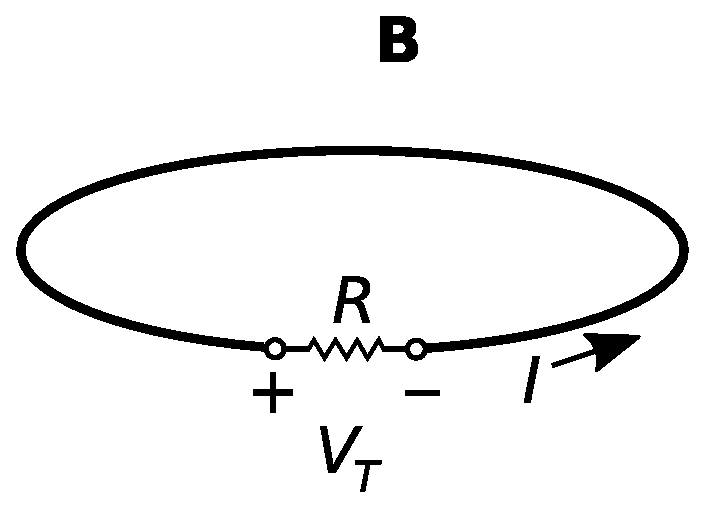
\includegraphics[width=2.5in]{modules/m0055_fFaradaySingleLoop.eps}
% ***WikipediaCommonsURL
}}{A loop of wire lying in a magnetic field, B. In the loop lies a resistor, R, between a positive and negative node. Beneath the resistor is labeled V sub T. A vector, I, on the right points in a counterclockwise direction.}
\end{center} 
%\centerline{\scriptsize 
%\copyright~\hyperref[***_Credit]{author} 
%\href{https://creativecommons.org/licenses/by-sa/4.0/}{CC BY-SA 4.0} 
%} 
\caption{
\label{m0056_fPS}
A single loop of wire in the presence of an impressed spatially-uniform but time-varying magnetic field.
}
\end{figure}

In the present problem, the loop is centered in the $z=0$ plane.
The magnetic flux density is ${\bf B} = \hat{\bf b}B(t)$; i.e., time-varying magnitude $B(t)$ and a constant direction $\hat{\bf b}$.
Because this magnetic field is spatially uniform (i.e., the same everywhere), we will find that only the area of the loop is important, and not it's specific shape.
For this reason, it will not be necessary to specify the radius of the loop or even require that it be a circular loop. 
Our task is to find expressions for $V_T$ and $I$.

To begin, remember that Faraday's Law is a calculation of electric potential and not current.
So, the approach is to first find $V_T$, and then find the current $I$ that flows through the gap resistance in response.
  
The sign convention for $V_T$ is arbitrary; here, we have selected ``$+$'' and ``$-$'' terminals as indicated in Figure~\ref{m0056_fPS}.\footnote{A good exercise for the student is to repeat this problem with the terminal polarity reversed; one should obtain the same answer.}
Following the standard convention for the reference direction of current through a passive device, $I$ should be directed as shown in Figure~\ref{m0056_fPS}.
It is worth repeating that these conventions for the signs of $V_T$ and $I$ are merely \emph{references}; for example, we may well find that $I$ is negative, which means that current flows in a clockwise direction in the loop. 

We now invoke Faraday's Law:
\index{Faraday's law}
%
\begin{equation}   
V_T = - N \frac{\partial}{\partial t} \Phi 
\end{equation}
%
The number of windings $N$ in the loop is 1, and $\Phi$ is the magnetic flux through the loop.  Thus:
%
\begin{equation}   
V_T = - \frac{\partial}{\partial t} \int_{\mathcal{S}} { {\bf B} \cdot d{\bf s} }
\end{equation}
%
where $\mathcal{S}$ is any open surface that intersects all of the magnetic field lines that pass through the loop.
The simplest such surface is simply the planar surface defined by the perimeter of the loop.
Then $d{\bf s}=\hat{\bf n}ds$, where $ds$ is the differential surface element and $\hat{\bf n}$ is the normal to the plane of the loop.
Which of the two possible normals to the loop?
This is determined by the right-hand rule 
\index{right-hand rule!Stokes' theorem}
of Stokes' Theorem.
\index{Stokes' theorem}
From the ``$-$'' terminal, we point the thumb of the right hand in the direction that leads to the ``$+$'' terminal by traversing the perimeter of the loop.
When we do this, the curled fingers of the right hand intersect $\mathcal{S}$ in the same direction as $\hat{\bf n}$.
To maintain the generality of results derived below, we shall not make the substitution $\hat{\bf n}=+\hat{\bf z}$; nevertheless we see this is the case for a loop parallel to the $z=0$ plane with the polarity of $V_T$ indicated in Figure~\ref{m0056_fPS}.

Taking this all into account, we have
%
\begin{flalign}   
V_T &= - \frac{\partial}{\partial t} \int_{\mathcal{S}} { \left(\hat{\bf b}B(t)\right) \cdot \left(\hat{\bf n}ds\right) } \nonumber \\
    &= - \left(\hat{\bf b}\cdot\hat{\bf n}\right) \frac{\partial}{\partial t} \int_{\mathcal{S}} {B(t)~ds } 
\end{flalign}
%
Since the magnetic field is uniform, $B(t)$ may be extracted from the integral.
Furthermore, the shape and the orientation of the loop are time-invariant, so the remaining integral may be extracted from the time derivative operation.
This leaves:
%
\begin{flalign}   
V_T = - \left(\hat{\bf b}\cdot\hat{\bf n}\right) \left( \frac{\partial}{\partial t} B(t) \right)  \int_{\mathcal{S}} { ds } 
\end{flalign}
%
The integral in this expression is simply the area of the loop, which is a constant; let the symbol $A$ represent this area.
We obtain
%
\begin{equation}  
\boxed{ 
V_T =  - \left(\hat{\bf b}\cdot\hat{\bf n}A\right) \frac{\partial}{\partial t} B(t)
}
\label{m0056_eVT}
\end{equation}
% 
which is the expression we seek.
Note that the quantity $\hat{\bf b}\cdot\hat{\bf n}A$ is the \emph{projected area} of the loop.
The projected area is equal to $A$ when the the magnetic field lines are perpendicular to the loop (i.e., $\hat{\bf b}=\hat{\bf n}$), and decreases to zero as $\hat{\bf b}\cdot\hat{\bf n}\to 0$.
Summarizing:
%
%ORB HIGHLIGHT
\begin{mdframed}[backgroundcolor=yellow!20,nobreak=true] 
The magnitude of the transformer emf induced by a spatially-uniform magnetic field is equal to the projected area times the time rate of change of the magnetic flux density, with a change of sign. (Equation~\ref{m0056_eVT}).
\end{mdframed}

A few observations about this result:  
%
\begin{itemize}
\item As promised earlier, we have found that the shape of the loop is irrelevant; i.e., a \emph{square} loop having the same area and planar orientation would result in the same $V_T$.  This is because the magnetic field is spatially uniform, and because it is the magnetic flux ($\Phi$) and not the magnetic field or shape of the loop alone that determines the induced potential. 
\item The induced potential is proportional to $A$; i.e., $V_T$ can be increased by increasing the area of the loop. 
\item The peak magnitude of the induced potential is maximized when the plane of the loop is perpendicular to the magnetic field lines.  
\item The induced potential goes to zero when the plane of the loop is parallel to the magnetic field lines.  Said another way, there is no induction unless magnetic field lines pass through the loop.   
\item The induced potential is proportional to the rate of change of ${\bf B}$.  If ${\bf B}$ is constant in time, then there is no induction.
\end{itemize}

Finally, the current in the loop is simply
%
\begin{equation}
I = \frac{V_T}{R}
\end{equation}
%
Again, electromagnetic induction induces potential, and the current flows only in response to the induced potential as determined by Ohm's Law.
In particular, if the resistor is removed, then $R\to\infty$ and $I\to0$, but $V_T$ is unchanged.

One final comment is that even though the current $I$ is not a \emph{direct} result of electromagnetic induction, we can use $I$ as a check of the result using Lenz's Law
\index{Lenz's law}
(Section~\ref{m0129_Electromagnetic_Induction}).  We'll demonstrate this in the example below.

%%%%%%%%%%%%%%%%%%%%%%%%%%%%%%%%%%%%%%%%%%%%%%%
%ORB EXAMPLE
~\\ \begin{example} 
\begin{mdframed}[backgroundcolor=brown!20,linecolor=brown!20]\raggedright
Induction in a motionless circular loop by a \emph{linearly}-increasing magnetic field
\\~\\
Let the loop be planar in the $z=0$ plane and circular with radius $a=10$~cm.
Let the magnetic field be $\hat{\bf z}B(t)$ where
%
\begin{flalign}
B(t) &=0       ~~~~~~~~\mbox{,}~t<0 \nonumber \\
     &=B_0 t/t_0 ~\mbox{,}~0\le t \le t_0 \nonumber \\
     &=B_0     ~~~~~~\mbox{,}~t>t_0 
\end{flalign}
%
i.e., $B(t)$ begins at zero and increases linearly to $B_0$ at time $t_0$, after which it remains constant at $B_0$.
Let $B_0=0.2$~T, $t_0=3$~s, and let the loop be closed by a resistor $R=1~\mbox{k}\Omega$.
What current $I$ flows in the loop? 

{\bf Solution}.   
Adopting the sign conventions of Figure~\ref{m0056_fPS} we first note that $\hat{\bf n}=+\hat{\bf z}$; this is determined by the right-hand rule with respect to the indicated polarity of $V_T$.
Thus, Equation~\ref{m0056_eVT} becomes
%
\begin{equation}  
V_T =  - \left(\hat{\bf b}\cdot\hat{\bf z}A\right) \frac{\partial}{\partial t} B(t)
\nonumber
\end{equation}
%
Note $\hat{\bf b}\cdot\hat{\bf z}A=A$ since $\hat{\bf b}=\hat{\bf z}$; i.e., because the plane of the loop is perpendicular to the magnetic field lines.
Since the loop is circular, $A = \pi a^2$. 
Also
%
\begin{flalign}
\frac{\partial}{\partial t}B(t) &=0       ~~~~~~~~\mbox{,}~t<0 \nonumber \\
                 &=B_0/t_0 ~\mbox{,}~0\le t \le t_0 \nonumber \\
                 &=0     ~~~~~~~\mbox{,}~t>t_0 \nonumber
\end{flalign}
%
Putting this all together:
%
\begin{equation}  
V_T =  -\pi a^2 \frac{B_0}{t_0} = -2.09~\mbox{mV} ~\mbox{,}~0\le t \le t_0
\nonumber
\end{equation}
%
and $V_T=0$ before and after this time interval, since ${\bf B}$ is constant during those times.
Subsequently the induced current is
%
\begin{equation}   
I = \frac{V_T}{R} = -2.09~\mu\mbox{A} ~\mbox{,}~0\le t \le t_0
\nonumber
\end{equation}
%
and $I=0$ before and after this time interval.
We have found that the induced current is a constant clockwise flow that exists only while ${\bf B}$ is increasing. 

Finally, let's see if the result is consistent with Lenz's Law.
\index{Lenz's law}
The current induced while ${\bf B}$ is changing gives rise to an induced magnetic field ${\bf B}_{ind}$.   
From the right-hand rule 
\index{right-hand rule!magnetic field of a wire}
that relates the direction of $I$  to the direction of ${\bf B}_{ind}$ (Section~\ref{m0119_Magnetic_Field_of_a_Long_Wire}), the direction of ${\bf B}_{ind}$ is generally $-\hat{\bf z}$ inside the loop.  
In other words, the magnetic field associated with the induced current opposes the increasing impressed magnetic field that induced the current, in accordance with Lenz's Law.  

\end{mdframed}
% note figures will need to go between "\end{mdframed}" and "\end{example}"
\end{example}
%%%%%%%%%%%%%%%%%%%%%%%%%%%%%%%%%%%%%%%%%%%%%%%

%%%%%%%%%%%%%%%%%%%%%%%%%%%%%%%%%%%%%%%%%%%%%%%
%ORB EXAMPLE
~\\ \begin{example} 
\begin{mdframed}[backgroundcolor=brown!20,linecolor=brown!20]\raggedright
Induction in a motionless circular loop by a \emph{sinusoidally}-varying magnetic field.
\\~\\
Let us repeat the previous example, but now with 
%
\begin{equation}
B(t) = B_0\sin{2\pi f_0 t}
\nonumber
\end{equation}
%
with $f_0=1$~kHz.

{\bf Solution}. 
Now
%
\begin{equation}   
\frac{\partial}{\partial t}B(t) = 2\pi f_0 B_0\cos{2\pi f_0 t}
\nonumber
\end{equation}
%
So
%
\begin{equation}  
V_T =  -2\pi^2 f_0 a^2 B_0  \cos{2\pi f_0 t}
\nonumber
\end{equation}
%
Subsequently
%
\begin{equation}   
I = \frac{V_T}{R} = -\frac{2\pi^2 f_0 a^2 B_0 }{R} \cos{2\pi f_0 t} 
\nonumber
\end{equation}
%
Substituting values, we have:
%
\begin{equation}   
I = -(39.5~\mbox{mA}) \cos{ \left[ (6.28~\mbox{krad/s}) t \right] } 
\nonumber
\end{equation}

It should be no surprise that $V_T$ and $I$ vary sinusoidally, since the source (${\bf B}$) varies sinusoidally.
A bit of useful trivia here is that $V_T$ and $I$ are 90$^{\circ}$ out of phase with the source.
It is also worth noting what happens when ${\bf B}(t)=0$.
This occurs twice per period, at $t=n/2f_0$ where $n$ is any integer, including $t=0$. 
At these times ${\bf B}(t)$ is zero, but $V_T$ and hence $I_R$ are decidedly non-zero; in fact, they are at their maximum magnitude.  
Again, it is the {\it change} in ${\bf B}$ that induces voltage and subsequently current, not ${\bf B}$ itself.

% Finally, let us see if the result is consistent with Lenz's Law. The induced current $I$ itself gives rise to a magnetic field.  For example, at $t=0$ (when ${\bf B}=0$) this current flows clockwise around the circuit.   From another ``right hand rule'', the reference direction of the associated magnetic field is $-\hat{\bf n}$ inside the loop.   This magnetic field persists, and points in the same direction, as the original magnetic field reemerges shortly after $t=0$.  At this time, the original and induced magnetic fields are pointing in opposite directions.  At time $t=1/4f_0$, the argument of $\sin$ is $\pi/2$ and original magnetic field begins to reduce, although it continues to point in the $+\hat{\bf z}$ direction.  However $I_R$ changes direction, and thus the induced magnetic field points in the $+\hat{\bf z}$ direction.  In other words: The magnetic field associated with the induced current opposes the change of the magnetic field that induces the current, which is Lenz's Law.  

%{\bf Example: Use of Lenz's Law to Determine the Direction of Current Flow.}
%Given the problem statement from the previous example, determine the direction of current flow at $t=1$~s.
%{\it Answer}: We already worked out that $d{\bf B}/dt=\hat{\bf z}2\pi f_0 B_0\cos{2\pi f_0 t}$. At $t=1$~s, $\cos{2\pi f_0 t}=1$, so at that time $d{\bf B}/dt$ is increasing in the $+\hat{\bf z}$ direction.  By Lenz's Law, the magnetic field induced by the current must be oriented in the $-\hat{\bf z}$ direction.  From the right hand rule, the direction of current flow must be counterclockwise. 

\end{mdframed}
% note figures will need to go between "\end{mdframed}" and "\end{example}"
\end{example}
%%%%%%%%%%%%%%%%%%%%%%%%%%%%%%%%%%%%%%%%%%%%%%%

\index{emf!transformer|)}

      \vfill\break
    \section{Transformers: Principle of Operation}
{\color{blue}\tiny[m0031]}      % This is text associated with the open textbook "Open Electromagnetics"
% See immediately below for author, date
% This work is licensed under the Creative Commons Attribution-ShareAlike 4.0 International License. (CC BY SA 4.0) 
% To view a copy of the license, visit http://creativecommons.org/licenses/by-sa/4.0/

%ORB TITLE Transformers: Principle of Operation
%ORB AUTHOR 0        # S.W. Ellingson, Virginia Tech (ellingson@vt.edu)
%ORB DATE 20180807   # yyyymmdd
%ORB ABSTRACT Transformers: Principle of Operation

\label{m0031_Transformers_Principle_of_Operation} % <-- Must match name of this file and module directory name.  Don't mess with this!
\index{transformer|(}

A transformer is a device that connects two electrical circuits through a shared magnetic field.  
Transformers are used in impedance transformation, voltage level conversion, circuit isolation, conversion between single-ended and differential signal modes, and other applications.\footnote{See ``Additional Reading'' at the end of this section for more on these applications.}
The underlying electromagnetic principle is Faraday's Law (Section~\ref{m0055_Faradays_Law}) -- in particular, transformer emf.

The essential features of a transformer can be derived from the simple experiment shown in Figures~\ref{m0031_fPoleTransformer1} and \ref{m0031_fPoleTransformer2}.  
In this experiment, two coils are arranged along a common axis.  
The winding pitch is small, so that all magnetic field lines pass through the length of the coil, and no lines pass between the windings.
To further contain the magnetic field, we assume both coils are wound on the same core, consisting of some material exhibiting high permeability. 
The upper coil has $N_1$ turns and the lower coil has $N_2$ turns. 

In Part~I of this experiment (Figure~\ref{m0031_fPoleTransformer1}), 
the upper coil is connected to a sinusoidally-varying voltage source $V_1^{(1)}$ in which the subscript refers to the coil and the superscript refers to ``Part~I'' of this experiment.
The voltage source creates a current in the coil, which in turn creates a time-varying magnetic field ${\bf B}$ in the core.  
%Applying the right-hand rule that relates current to induced magnetic field, the reference direction for ${\bf B}$ is in the downward ($-\hat{\bf z}$) direction.
%
\begin{figure}
\begin{center}
\pdftooltip{{  % note double braces
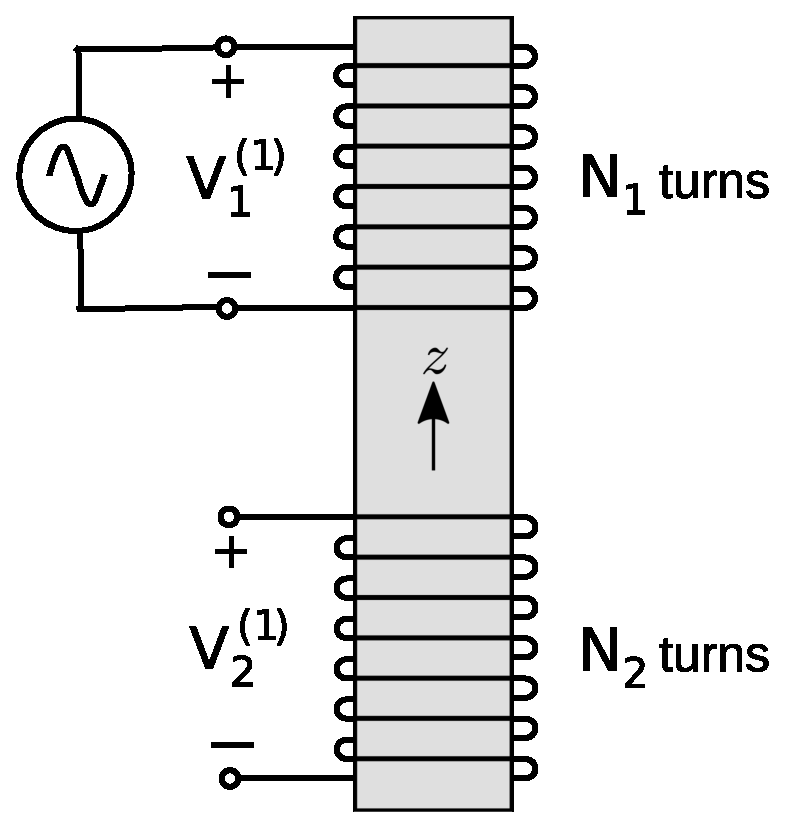
\includegraphics[width=2in]{modules/m0031_fPoleTransformer1.eps}
}}{A long rectangle with two separate groups of wire. The upper uniformly wound coil is labeled N sub 1 turns. An AC voltage source is connected to either side of the coil and labeled V sub 1 super (1). On the second coil, labeled N sub 2 turns, are 2 nodes labeled V sub 2 super (1). In both cases the positive node is above the negative node. A vector in the middle of the rectangular axis is labeled z.}
\end{center} 
\caption{\label{m0031_fPoleTransformer1} Part I of an experiment demonstrating the linking of electric circuits using a transformer.}
\end{figure}
%
\begin{figure}
\begin{center}
\pdftooltip{{  % note double braces
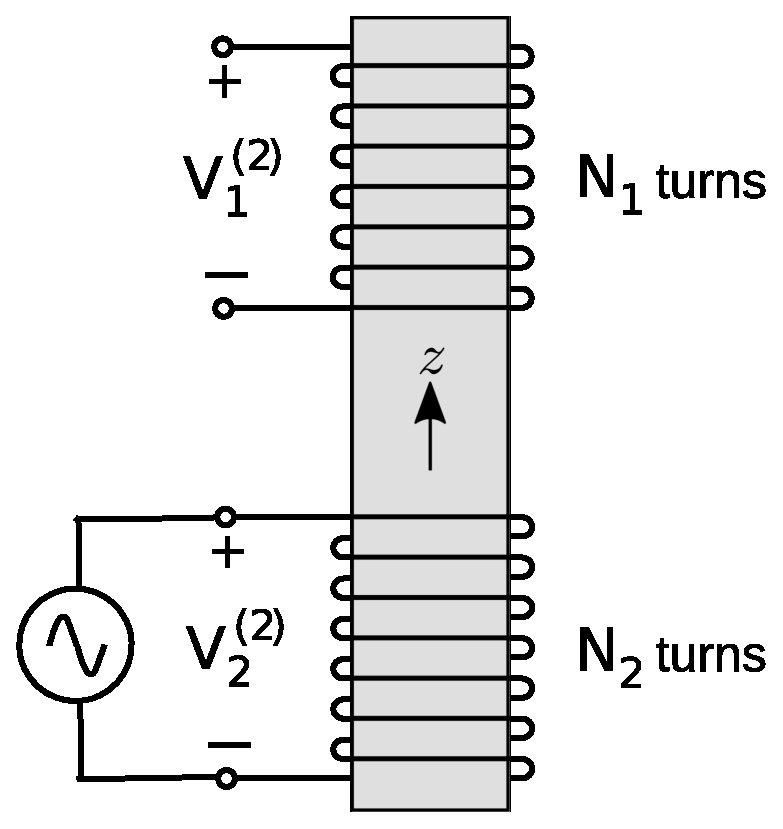
\includegraphics[width=2in]{modules/m0031_fPoleTransformer2.eps}
}}{Similar to previous figure, but flipped across the horizontal. V sub 2 is connected to an AC source and V sub 1 is an open circuit. A vector in the middle of the rectangular axis is labeled z. }
\end{center} 
\caption{\label{m0031_fPoleTransformer2} Part II of an experiment demonstrating the linking of electric circuits using a transformer.}
\end{figure} 

The lower coil has $N_2$ turns wound in the \emph{opposite direction} and is open-circuited.
Given the closely-spaced windings and use of a high-permeability core, we assume that the magnetic field within the lower coil is equal to ${\bf B}$ generated in the upper coil.  The potential induced in the lower coil is $V_2^{(1)}$ with reference polarity indicated in the figure.  
From Faraday's Law we have
%
\begin{equation}   
V_2^{(1)} = - N_2 \frac{\partial}{\partial t} \Phi_2
\label{m0031_ePartIa}
\end{equation}
%
where $\Phi_2$ is the flux through a single turn of the lower coil.  Thus:
%
\begin{equation}   
V_2^{(1)} = -N_2 \frac{\partial}{\partial t} \int_{\mathcal{S}} { {\bf B} \cdot (-\hat{\bf z}ds) }
\label{m0031_ePartIb}
\end{equation}
%
Note that the direction of $d{\bf s}=-\hat{\bf z}ds$ is determined by the polarity we have chosen for $V_2^{(1)}$.

In Part~II of the experiment (Figure~\ref{m0031_fPoleTransformer2}), we make changes as follows. We apply a voltage $V_2^{(2)}$ to the lower coil and open-circuit the upper coil. Further, we adjust $V_2^{(2)}$ such that the induced magnetic flux density is again ${\bf B}$ -- that is, equal to the field in Part~I of the experiment.  Now we have
%
\begin{equation}   
V_1^{(2)} = - N_1 \frac{\partial}{\partial t} \Phi_1 
\end{equation}
%
which is
%
\begin{equation}   
V_1^{(2)} = -N_1 \frac{\partial}{\partial t} \int_{\mathcal{S}} { {\bf B} \cdot (+\hat{\bf z}ds) }
\end{equation}
%
For reasons that will become apparent in a moment, let's shift the leading minus sign into the integral.  We then have
%
\begin{equation}   
V_1^{(2)} = +N_1 \frac{\partial}{\partial t} \int_{\mathcal{S}} { {\bf B} \cdot (-\hat{\bf z}ds) }
\end{equation}
%
Comparing this to Equations~\ref{m0031_ePartIa} and \ref{m0031_ePartIb}, we see that we may rewrite this in terms of the flux in the lower coil in Part~I of the experiment:
%
\begin{equation}   
V_1^{(2)} = +N_1 \frac{\partial}{\partial t} \Phi_2
\end{equation}
%
In fact, we can express this in terms of the \emph{potential} in Part~I of the experiment:
%
\begin{flalign}   
V_1^{(2)} &= \left(-\frac{N_1}{N_2}\right) \left(-N_2 \frac{\partial}{\partial t} \Phi_2 \right) \nonumber \\
          &= \left(-\frac{N_1}{N_2}\right) V_2^{(1)} 
\end{flalign}
%
We have found that the potential in the upper coil in Part~II is related in a simple way to the potential in the lower coil in Part~I of the experiment.
If we had done Part~II first, we would have obtained the same result but with the superscripts swapped.  
Therefore, it must be generally true -- regardless of the arrangement of terminations -- that 
%
\begin{equation}   
V_1 = -\frac{N_1}{N_2}V_2
\end{equation}
%
This expression should be familiar from elementary circuit theory -- except possibly for the minus sign.
The minus sign is a consequence of the fact that the coils are wound in opposite directions.  
We can make the above expression a little more general as follows:  
%
\begin{equation}   
\boxed{
\frac{V_1}{V_2} = p\frac{N_1}{N_2}
}
\label{m0031_eTL}
\end{equation}
%
where $p$ is defined to $+1$ when the coils are wound in the same direction and $-1$ when coils are wound in opposite directions. 
(It is an excellent exercise to confirm that this is true by repeating the above analysis with winding direction changed for either the upper or lower coil, for which $p$ will then turn out to be $+1$.)  
This is the ``transformer law'' of basic electric circuit theory, from which all other characteristics of transformers as two-port circuit devices can be obtained (See Section~\ref{m0032_Transformers_as_Two-Port_Devices} for follow-up on that).  
Summarizing:
%
%ORB HIGHLIGHT
\begin{mdframed}[backgroundcolor=yellow!20,nobreak=true] 
The ratio of coil voltages in an ideal transformer is equal to the ratio of turns with sign determined by the relative directions of the windings, per Equation~\ref{m0031_eTL}.
\end{mdframed}

A more familiar transformer design is shown in Figure~\ref{m0031_fTransformer3d_col3} -- coils wound on a toroidal core as opposed to a cylindrical core.
Why do this?
This arrangement confines the magnetic field linking the two coils to the core, as opposed to allowing field lines to extend beyond the device.
This confinement is important in order to prevent fields originating outside the transformer from interfering with the magnetic field linking the coils, which would lead to electromagnetic interference (EMI)
\index{electromagnetic interference (EMI)}
and electromagnetic compatibility (EMC) 
\index{electromagnetic compatibility (EMC)}
problems.
The principle of operation is in all other respects the same.
%
\begin{figure}
\begin{center}
\pdftooltip{{  % note double braces
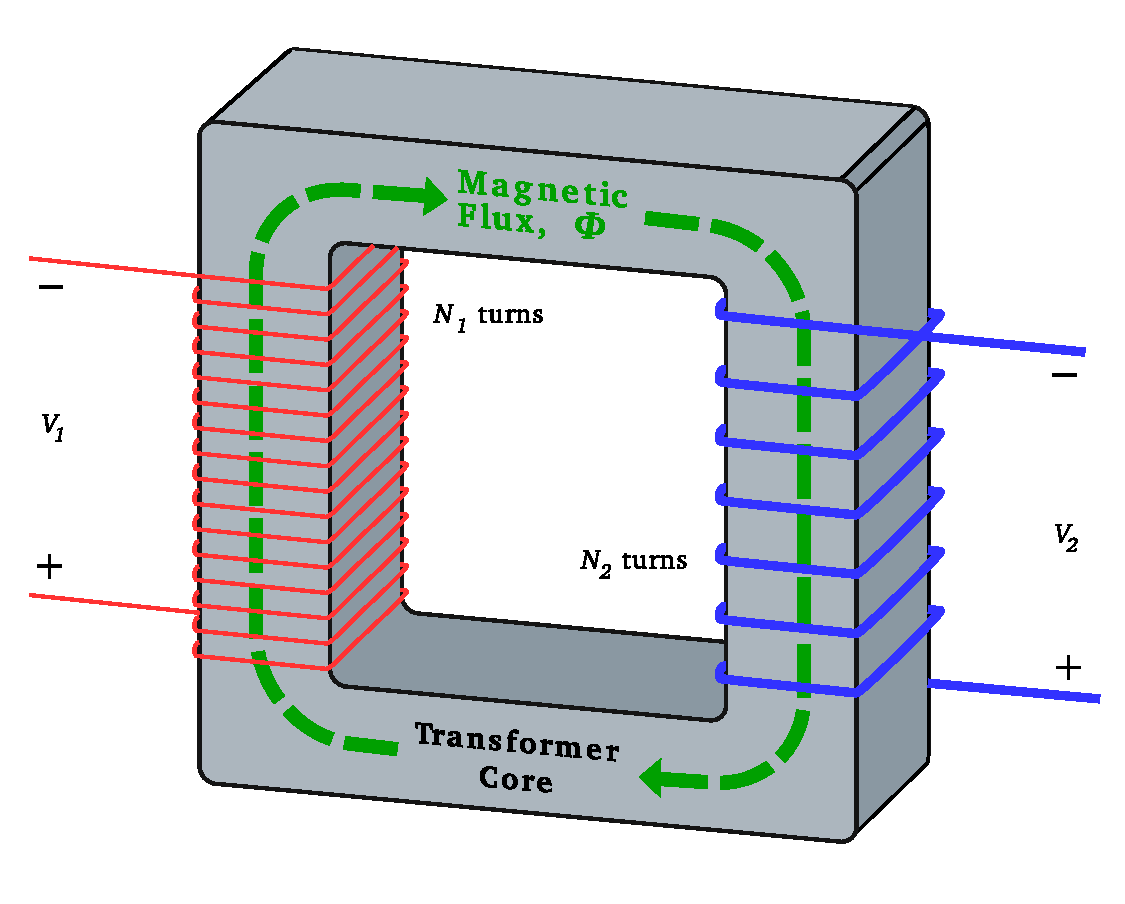
\includegraphics[width=\columnwidth]{modules/m0031_fTransformer3d_col3.eps}
% https://commons.wikimedia.org/wiki/File:Transformer3d_col3.svg
}}{A three dimensional cube with the middle cut out, representing a toroidal core and at the bottom labeled "Transformer Core". Within the core is a green dashed arrow going all the way around, pointed in a clockwise direction and labeled magnetic flux, Phi. On the left side of the core is a red coil with thin, uniform, N sub 1 turns. The top end is negative, and the bottom is positive. Between the ends is labeled V sub 1. On the right side of the core is a blue coil with more widely spaced, uniform N sub 2 turns. The top end is negative, and the bottom is positive. Between the ends is labeled V sub 2. }
\end{center} 
\centerline{\scriptsize 
\copyright~\hyperref[m0031_fTransformer3d_col3_Credit]{BillC} (modified) 
\href{https://creativecommons.org/licenses/by-sa/3.0/}{CC BY~SA 3.0} 
} 
\caption{
\label{m0031_fTransformer3d_col3}
Transformer implemented as coils sharing a toroidal core.  Here $p=+1$.
}
\end{figure}

%%%%%%%%%%%%%%%%%%%%%%%%%%%%%%%%%%%%%%%%%%%%%%%%%%%%%%%%%%%%%%%%%%%%%%

{\bf Additional Reading:}
\begin{itemize}
\item ``\href{https://en.wikipedia.org/wiki/Transformer}{Transformer}'' on Wikipedia.
\item ``\href{https://en.wikipedia.org/wiki/Balun}{Balun}'' on Wikipedia.
\end{itemize}

\index{transformer|)}

      \vfill\break
    \section{Transformers as Two-Port Devices}
{\color{blue}\tiny[m0032]}      % This is text associated with the open textbook "Open Electromagnetics"
% See immediately below for author, date
% This work is licensed under the Creative Commons Attribution-ShareAlike 4.0 International License. (CC BY SA 4.0) 
% To view a copy of the license, visit http://creativecommons.org/licenses/by-sa/4.0/

%ORB TITLE Transformers as Two-Port Devices
%ORB AUTHOR 0        # S.W. Ellingson, Virginia Tech (ellingson@vt.edu)
%ORB DATE 20180807   # yyyymmdd
%ORB ABSTRACT Transformers as Two-Port Devices

\label{m0032_Transformers_as_Two-Port_Devices} % <-- Must match name of this file and module directory name.  Don't mess with this!
\index{transformer|(}

Section~\ref{m0031_Transformers_Principle_of_Operation} explains the principle of operation of the ideal transformer.
The relationship governing the terminal voltages $V_1$ and $V_2$ was found to be
%
\begin{equation}   
\frac{V_1}{V_2} = p\frac{N_1}{N_2}
\end{equation}
%
where $N_1$ and $N_2$ are the number of turns in the associated coils and $p$ is either $+1$ or $-1$ depending on the relative orientation of the windings; i.e., whether the reference direction of the associated fluxes is the same or opposite, respectively. 
 
We shall now consider ratios of current and impedance in ideal transformers, using the two-port model shown in Figure~\ref{m0032_f2P}.  
By virtue of the reference current directions and polarities chosen in this figure, the power delivered by the source $V_1$ is $V_1 I_1$, and the power absorbed by the load $Z_2$ is $-V_2 I_2$.  Assuming the transformer windings have no resistance, and assuming the magnetic flux is perfectly contained within the core, the power absorbed by the load must equal the power provided by the source; i.e., $V_1 I_1 = -V_2 I_2$.  Thus, we have\footnote{
The minus signs in this equation are a result of the reference polarity and directions indicated in Figure~\ref{m0032_f2P}.
These are more-or-less standard in electrical two-port theory (see ``Additional Reading'' at the end of this section), but are certainly not the only reasonable choice.
If you see these expressions without the minus signs, it probably means that a different combination of reference directions/polarities is in effect.
} % \footnote
%
\begin{equation}   
\boxed{
\frac{I_1}{I_2} = -\frac{V_2}{V_1} = -p\frac{N_2}{N_1}
}
\end{equation}
%
\begin{figure}[b!]
\begin{center}
\pdftooltip{{  % note double braces
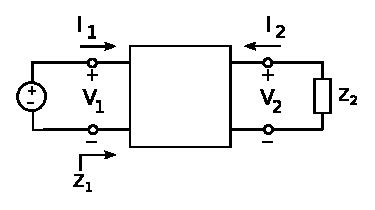
\includegraphics[width=2.5in]{modules/m0032_f2P.eps}
}}{A transformer between two circuits, one on the left and one on the right. In the left circuit is an independent voltage source between a positive and negative node. Between the nodes is labeled V sub 1. From the positive node, I sub 1 is shown going into the transformer. From the negative node Z sub 1 is shown going into the transformer. In the right circuit is an impedance, Z sub 2, between a positive and negative node labeled V sub 2.  From the positive node, I sub 2 is shown going into the transformer.}
\end{center} 
\caption{\label{m0032_f2P} The transformer as a two-port circuit device.}
\end{figure} 

We can develop an impedance relationship for ideal transformers as follows. 
Let $Z_1$ be the input impedance of the transformer; that is, the impedance looking into port~1 from the source.
Thus, we have
%
\begin{flalign}
Z_1 &\triangleq \frac{V_1}{I_1} \nonumber \\ 
    &= \frac{+p\left(N_1/N_2\right)V_2}{-p\left(N_2/N_1\right)I_2} \nonumber \\
    &= -\left(\frac{N_1}{N_2}\right)^2\left(\frac{V_2}{I_2}\right)
\end{flalign}
%
In Figure~\ref{m0032_f2P}, $Z_2$ is the the output impedance of port 2; that is, the impedance looking out port 2 into the load.
Therefore, $Z_2 = -V_2/I_2$ (once again the minus sign is a result of our choice of sign conventions in Figure~\ref{m0032_f2P}).
Substitution of this result into the above equation yields
%
\begin{equation}
Z_1 = \left(\frac{N_1}{N_2}\right)^2 Z_2
\end{equation}
%
and therefore
%
\begin{equation}
\boxed{
\frac{Z_1}{Z_2} = \left(\frac{N_1}{N_2}\right)^2 
}
\end{equation}
%
Thus, we have demonstrated that a transformer scales impedance in proportion to the square of the turns ratio $N_1/N_2$.
Remarkably, the impedance transformation depends \emph{only} on the turns ratio, and is independent of the relative direction of the windings ($p$). 

%The voltage ratio, current ratio, and impedance ratio laws for ideal transformers are often sufficient for analysis and design of circuits using practical transformers.  Sometimes however the non-ideal aspects of transformers must be also be considered.  
%There are two mechanisms which may impact the performance of a transformer:  {\it Winding capacitance} and {\it stray inductance}.  These additional mechanisms are indicated in the equivalent circuit shown in Figure~\ref{fTF-DCM} as $C_{ic}$ and $L_{stray}$ respectively.  Winding capacitance is due to the storage of electric energy in the space between the individual turns of the coil.   
%Stray inductance results from the imperfect containment of the magnetic flux.  
%In particular, magnetic flux generated near the ends of the coils may exist in small loops that do not pass through the other coil, in which case that portion of the coil is behaving as a simple inductor as opposed to a transformer.  
%%
%\begin{figure}
%%\begin{center}\psfig{file=figs/101025_LWA1_HighRes_trim.eps,width=6.3in}\end{center} 
%\vspace{3in}
%\caption{\label{m0032_f2PEC} Circuit model for a transformer including winding capacitance and stray inductance.}
%\end{figure} 

The relationships developed above should be viewed as AC expressions, and are not normally valid at DC.
This is because transformers exhibit a fundamental limitation in their low-frequency performance.
To see this, first recall Faraday's Law:
%
\begin{equation}   
V = - N \frac{\partial}{\partial t} \Phi
\end{equation}
%
If the magnetic flux $\Phi$ isn't time-varying, then there is no induced electric potential, and subsequently no linking of the signals associated with the coils.
At very low but non-zero frequencies, we encounter another problem that gets in the way -- \emph{magnetic saturation}.
\index{saturation (magnetic)}
To see this, note we can obtain an expression for $\Phi$ from Faraday's Law by integrating with respect to time, yielding
%
\begin{equation}
\Phi(t) = -\frac{1}{N}\int_{t_0}^{t}V(\tau)d\tau + \Phi(t_0)   
\end{equation}
%
where 
$t_0$ is some earlier time at which we know the value of $\Phi(t_0)$.
Let us assume that $V(t)$ is sinusoidally-varying.
Then the peak value of $\Phi$ after $t=t_0$ depends on the frequency of $V(t)$.  
If the frequency of $V(t)$ is very low, then $\Phi$ can become very large.  Since the associated cross-sectional areas of the coils are presumably constant, this means that the magnetic field becomes very large.  The problem with that is that most practical high-permeability materials suitable for use as transformer cores exhibit magnetic saturation; that is, the rate at which the magnetic field is able to increase decreases with increasing magnetic field magnitude (see Section~\ref{m0058_Magnetic_Materials}).  
The result of all this is that a transformer may work fine at (say) 1~MHz, but at (say) 1~Hz the transformer may exhibit an apparent loss associated with this saturation.  Thus, practical transformers exhibit highpass frequency response. 

It should be noted that the highpass behavior of practical transistors can be useful. For example, a transformer can be used to isolate an undesired DC offset and/or low-frequency noise in the circuit attached to one coil from the circuit attached to the other coil.  

The DC-isolating behavior of a transformer also allows the transformer to be used as a \emph{balun}, 
\index{balun}
as illustrated in Figure~\ref{m0032_fBalun}.  A balun is a two-port device that transforms a single-ended (``unbalanced'') signal -- that is, one having an explicit connection to a datum (e.g., ground) -- into a differential (``balanced'') signal, for which there is no explicit connection to a datum.  Differential signals have many benefits in circuit design, whereas inputs and outputs to devices must often be in single-ended form.
Thus, a common use of transformers is to effect the conversion between single-ended and differential circuits.
Although a transformer is certainly not the only device that can be used as a balun, it has one very big advantage, namely bandwidth.
%
\begin{figure}
\begin{center}
\pdftooltip{{  % note double braces
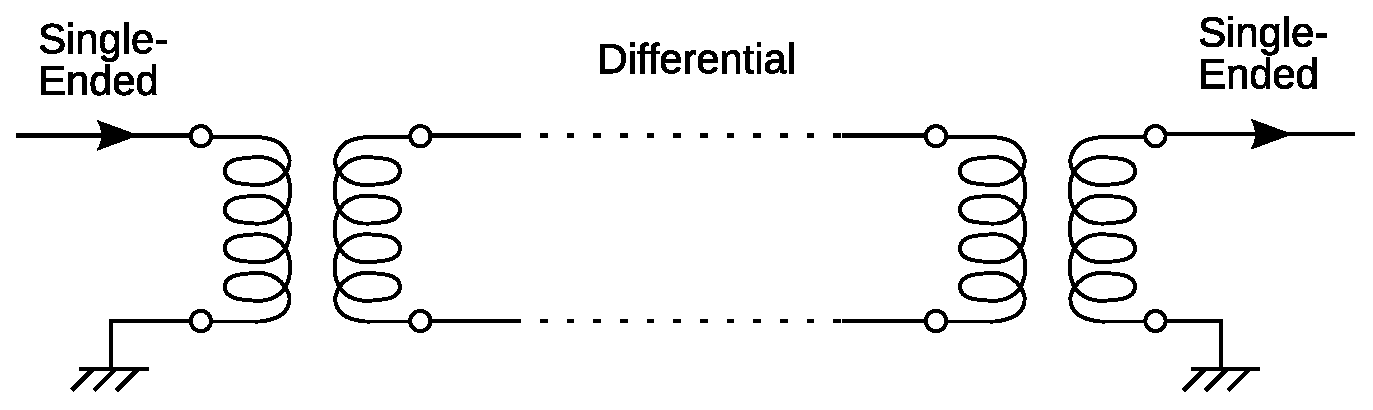
\includegraphics[width=\columnwidth]{modules/m0032_fBalun.eps}
% https://en.wikipedia.org/wiki/File:Transformer_balance.svg
}}{A single-ended coil has current entering the top and the bottom is connected to ground. To its right is a second coil connected to a third coil by a dashed line and labeled differential. To the right of the “differential” is a final single-ended coil with current exiting to the top and grounded at the bottom.}
\end{center} 
\centerline{\scriptsize 
\copyright~\hyperref[m0032_fBalun_Credit]{SpinningSpark} 
\href{https://creativecommons.org/licenses/by-sa/3.0/}{CC BY~SA 3.0} 
(modified)
} 
\caption{
\label{m0032_fBalun}
Transformers used to convert a single-ended (``unbalanced'') signal to a differential (balanced) signal, and back.
}
\end{figure}

%%%%%%%%%%%%%%%%%%%%%%%%%%%%%%%%%%%%%%%%%%%%%%%%%%%%%%%%%%%%%%%%%%%%%%

{\bf Additional Reading:}
\begin{itemize}
\item ``\href{https://en.wikipedia.org/wiki/Transformer}{Transformer}'' on Wikipedia.
\item ``\href{https://en.wikipedia.org/wiki/Two-port_network}{Two-port network}'' on Wikipedia.
\item ``\href{https://en.wikipedia.org/wiki/Saturation_(magnetic)}{Saturation (magnetic)}'' on Wikipedia.
\item ``\href{https://en.wikipedia.org/wiki/Balun}{Balun}'' on Wikipedia.
\item S.W. Ellingson, ``Differential Circuits'' (Sec.~8.7) in \emph{Radio Systems Engineering}, Cambridge Univ.\ Press, 2016.
\end{itemize}

\index{transformer|)}

      \vfill\break
    \section{The Electric Generator}
{\color{blue}\tiny[m0030]}      % This is text associated with the open textbook "Open Electromagnetics"
% See immediately below for author, date
% This work is licensed under the Creative Commons Attribution-ShareAlike 4.0 International License. (CC BY-SA 4.0) 
% To view a copy of the license, visit http://creativecommons.org/licenses/by-sa/4.0/

%ORB TITLE The Electric Generator
%ORB AUTHOR 0        # S.W. Ellingson, Virginia Tech (ellingson@vt.edu)
%ORB DATE 20180807   # yyyymmdd
%ORB ABSTRACT The Electric Generator

\label{m0030_Electric_Generator} % <-- Must match name of this file and module directory name.  Don't mess with this!
\index{generator|(}

A generator is a device that transforms mechanical energy into electrical energy, typically by electromagnetic induction via Faraday's Law (Section~\ref{m0055_Faradays_Law}).
For example, a generator might consist of a gasoline engine that turns a crankshaft to which is attached a system of coils and/or magnets.  This rotation changes the relative orientations of the coils with respect to the magnetic field in a time-varying manner, resulting in a time-varying magnetic flux and subsequently induced electric potential.
In this case, the induced potential is said to be a form of \emph{motional emf}, 
\index{emf!motional}
as it is due entirely to changes in geometry as opposed to changes in the magnitude of the magnetic field.
Coal- and steam-fired generators, hydroelectric generators, wind turbines, and other energy generation devices operate using essentially this principle.

Figure~\ref{m0030_fGen} shows a rudimentary generator, which serves as to illustrate the relevant points.
This generator consists of a planar loop that rotates around the $z$ axis; therefore, the rotation can be parameterized in $\phi$.
In this case, the direction of rotation is specified to be in the $+\phi$ direction.
The frequency of rotation is $f_0$; that is, the time required for the loop to make one complete revolution is $1/f_0$.
We assume a time-invariant and spatially-uniform magnetic flux density ${\bf B}=\hat{\bf b}B_0$ where $\hat{\bf b}$ and $B_0$ are both constants.
For illustration purposes, the loop is indicated to be circular. 
However, because the magnetic field is time-invariant and spatially-uniform, the specific shape of the loop is not important, as we shall see in a moment.  Only the area of the loop will matter.
%
\begin{figure}
\begin{center}
\pdftooltip{{  % note double braces
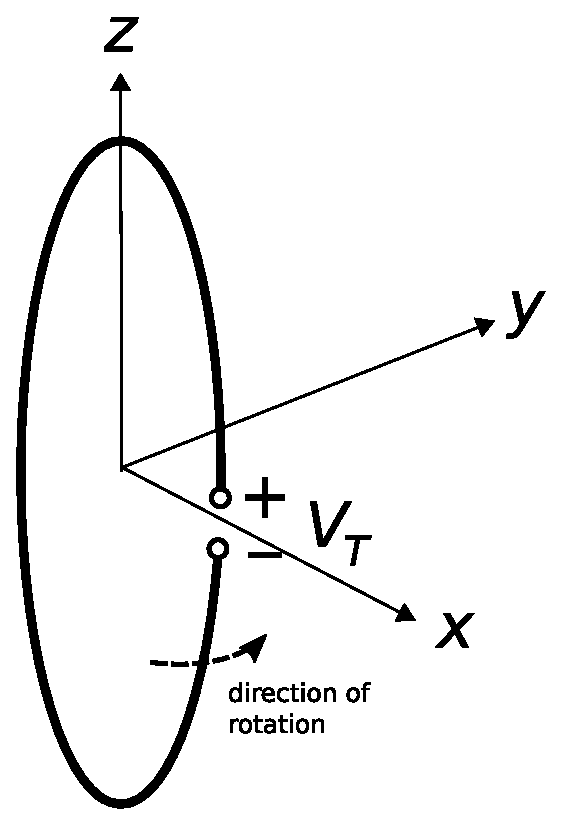
\includegraphics[width=2in]{modules/m0030_fGen.eps}
% ***WikipediaCommonsURL
}}{A single loop generator lying on a three dimensional Cartesian coordinate system, with the z-axis pointed up. On the loop on either side of the x-axis has open nodes, the top positive and the bottom negative. It is labeled V sub T. A dashed arrow curves out of the middle of the loop slightly upward, labeled "direction of rotation".}
\end{center} 
%\centerline{\scriptsize 
%\copyright~\hyperref[***_Credit]{author} 
%\href{https://creativecommons.org/licenses/by-sa/4.0/}{CC BY-SA 4.0} 
%} 
\caption{
\label{m0030_fGen}
A rudimentary single-loop generator, shown at time $t=0$.
}
\end{figure}

The induced potential is indicated as $V_T$ with reference polarity as indicated in the figure.
This potential is given by Faraday's Law:
%
\begin{equation}   
V_T = - \frac{\partial}{\partial t} \Phi
\end{equation}
%
Here $\Phi$ is the magnetic flux associated with an open surface $\mathcal{S}$ bounded by the loop:
%
\begin{equation}   
\Phi = \int_{\mathcal{S}} { {\bf B} \cdot d{\bf s} }
\end{equation}
%
As usual, $\mathcal{S}$ can be any surface that intersects all magnetic field lines passing through the loop, and also as usual, the simplest choice is simply the planar area bounded by the loop.
The differential surface element $d{\bf s}$ is $\hat{\bf n}ds$, where $\hat{\bf n}$ is determined by the reference polarity of $V_T$ according to the ``right hand rule'' convention from Stokes' Theorem.
Making substitutions, we have
%
\begin{flalign}   
\Phi &= \int_{\mathcal{S}} { \left(\hat{\bf b}B_0\right) \cdot \left(\hat{\bf n}ds\right) } \nonumber \\
     &= \left[\hat{\bf b}\cdot\hat{\bf n}\right]B_0 \int_{\mathcal{S}} ds  \nonumber \\
     &= \left[\hat{\bf b}\cdot\hat{\bf n}A\right] B_0 
\end{flalign}
%
where $A$ is the area of the loop.

To make headway, an expression for $\hat{\bf n}$ is needed.
The principal difficulty here is that $\hat{\bf n}$ is rotating with the loop, so it is time-varying.
To sort this out, first consider the situation at time $t=0$, which is the moment illustrated in Figure~\ref{m0030_fGen}.
Beginning at the ``$-$'' terminal, we point the thumb of our right hand in the direction that leads to the ``$+$'' terminal by traversing the loop; $\hat{\bf n}$ is then the direction perpendicular to the plane of the loop in which the fingers of our right hand pass through the loop.  
We see that at $t=0$, $\hat{\bf n}=+\hat{\bf y}$.
A bit later, the loop will have rotated by one-fourth of a complete rotation, and at that time $\hat{\bf n}=-\hat{\bf x}$.
This occurs at $t=1/(4f_0)$.
Later still, the loop will have rotated by one-half of a compete rotation, and then $\hat{\bf n}=-\hat{\bf y}$.
This occurs at $t=1/(2f_0)$.
It is apparent that
%
\begin{equation}
\hat{\bf n}(t) = -\hat{\bf x}\sin 2\pi f_0 t +\hat{\bf y}\cos 2\pi f_0 t
\end{equation}
%
as can be confirmed by checking the three special cases identified above.
Now applying Faraday's Law, we find
%
\begin{flalign}
V_T &= - \frac{\partial}{\partial t} \Phi \nonumber \\
    &= - \frac{\partial}{\partial t} \left[\hat{\bf b}\cdot\hat{\bf n}(t)\right]A B_0 \nonumber \\
    &= - \left[\hat{\bf b}\cdot\frac{\partial}{\partial t}\hat{\bf n}(t)\right]A B_0 
\end{flalign}
%
For notational convenience we make the following definition:
%
\begin{equation}
\hat{\bf n}'(t) \triangleq -\frac{1}{2\pi f_0}\frac{\partial}{\partial t}\hat{\bf n}(t)
\label{m0030_eEGrho}
\end{equation}
%
which is simply the time derivative of $\hat{\bf n}$ divided by $2\pi f_0$ so as to retain a unit vector.  The reason for including a change of sign will become apparent in a moment.
Applying this definition, we find
%
\begin{equation}
\hat{\bf n}'(t) = +\hat{\bf x}\cos 2\pi f_0 t +\hat{\bf y}\sin 2\pi f_0 t
\end{equation}
%
Note that this is essentially the definition of the radial basis vector $\hat{\bf \rho}$ from the cylindrical coordinate system (which is why we applied the minus sign in Equation~\ref{m0030_eEGrho}).  
Recognizing this, we write
%
\begin{equation}
\hat{\bf \rho}(t) = +\hat{\bf x}\cos 2\pi f_0 t +\hat{\bf y}\sin 2\pi f_0 t
\end{equation}
%
and finally
%
\begin{equation}   
\boxed{
V_T = +2\pi f_0 A B_0 \hat{\bf b}\cdot\hat{\bf \rho}(t) 
}
\label{m0030_eGen} 
\end{equation}

If the purpose of this device is to generate power, then presumably we would choose the magnetic field to be in a direction that maximizes the maximum value of $\hat{\bf b}\cdot\hat{\bf \rho}(t)$.
Therefore, power is optimized for ${\bf B}$ polarized entirely in some combination of $\hat{\bf x}$ and $\hat{\bf y}$, and with ${\bf B}\cdot\hat{\bf z}=0$. 
Under that constraint, we see that $V_T$ varies sinusoidally with frequency $f_0$ and exhibits peak magnitude 
%
\begin{equation}  
\boxed{ 
\mbox{max}~\left|V_T(t)\right| = 2\pi f_0 A B_0 
}
\end{equation}
%
It's worth noting that the maximum voltage magnitude is achieved when the plane of the loop is parallel to ${\bf B}$; i.e., when $\hat{\bf b}\cdot\hat{\bf n}(t)=0$ so that $\Phi(t)=0$.  Why is that?  Because this is when $\Phi(t)$ is most rapidly increasing or decreasing.
Conversely, when the plane of the loop is perpendicular to ${\bf B}$ (i.e., $\hat{\bf b}\cdot\hat{\bf n}(t)=1$), $\left|\Phi(t)\right|$ is maximum but its time-derivative is zero, so $V_T(t)=0$ at this instant.

%%%%%%%%%%%%%%%%%%%%%%%%%%%%%%%%%%%%%%%%%%%%%%%
%ORB EXAMPLE
~\\ \begin{example} 
\begin{mdframed}[backgroundcolor=brown!20,linecolor=brown!20]\raggedright
Rudimentary electric generator.
\\~\\
The generator in Figure~\ref{m0030_fGen} consists of a circular loop of radius $a=1$~cm rotating at 1000 revolutions per second in a static and spatially-uniform magnetic flux density of 1~mT in the $+\hat{\bf x}$ direction.
What is the induced potential?

{\bf Solution.}
From the problem statement, $f_0=1$~kHz, $B_0=1$~mT, and $\hat{\bf b}=+\hat{\bf x}$.
Therefore $\hat{\bf b}\cdot\hat{\bf \rho}(t)$ $=$ $\hat{\bf x}\cdot\hat{\bf \rho}(t)$ $=$ $\cos 2\pi f_0 t$.
The area of the loop is $A=\pi a^2$.
From Equation~\ref{m0030_eGen} we obtain 
%
\begin{equation}
V_T(t) \cong \left(1.97~\mbox{mV}\right)\cos\left[\left(6.28~\mbox{krad/s}\right)t\right] 
\nonumber
\end{equation}
\end{mdframed}
\end{example}
%%%%%%%%%%%%%%%%%%%%%%%%%%%%%%%%%%%%%%%%%%%%%%%

Finally, we note that it is not really necessary for the loop to rotate in the presence of a magnetic field with constant $\hat{\bf b}$; it works equally well for the loop to be stationary and for $\hat{\bf b}$ to rotate -- in fact, this is essentially the same problem.  In some practical generators, both the potential-generating coils and fields (generated by some combination of magnets and coils) rotate.


{\bf Additional Reading:}
\begin{itemize}
\item ``\href{https://en.wikipedia.org/wiki/Electric_generator}{Electric Generator}'' on Wikipedia.
%\item \href{https://en.wikipedia.org/wiki/Electric_motor}{Electric Motor} on Wikipedia.
\end{itemize}

\index{generator|)}

      \vfill\break
    \section{The Maxwell-Faraday Equation}
{\color{blue}\tiny[m0050]}      % This is text associated with the open textbook "Open Electromagnetics"
% See immediately below for author, date
% This work is licensed under the Creative Commons Attribution-ShareAlike 4.0 International License. (CC BY SA 4.0) 
% To view a copy of the license, visit http://creativecommons.org/licenses/by-sa/4.0/

%ORB TITLE The Maxwell-Faraday Equation 
%ORB AUTHOR 0        # S.W. Ellingson, Virginia Tech (ellingson@vt.edu)
%ORB DATE 20180807   # yyyymmdd
%ORB ABSTRACT The Maxwell-Faraday Equation 

\label{m0050_Maxwell-Faraday_Equation} % <-- Must match name of this file and module directory name.  Don't mess with this!
\index{Maxwell-Faraday equation|(}

In this section, we generalize Kirchoff's Voltage Law (KVL), 
\index{Kirchoff's voltage law!electrostatics}
previously encountered as a principle of electrostatics in Sections~\ref{m0016_Kirchoffs_Voltage_Law_Electrostatics_Integral_Form} and \ref{m0152_KVL_Electrostatics_Integral-to-Differential}.
KVL states that in the absence of a time-varying magnetic flux, the electric potential accumulated by traversing a closed path $\mathcal{C}$ is zero.
Here is that idea in mathematical form:
%
\begin{equation}   
V = \oint_{\mathcal{C}}{ {\bf E} \cdot d{\bf l} } = 0
\end{equation}
%
Now recall Faraday's Law 
\index{Faraday's law}
(Section~\ref{m0055_Faradays_Law}): 
%
\begin{equation}
V = - \frac{\partial}{\partial t} \Phi = - \frac{\partial}{\partial t} \int_{\mathcal{S}} { {\bf B} \cdot d{\bf s} }
\end{equation}
%
Here, $\mathcal{S}$ is any open surface that intersects all magnetic field lines passing through $\mathcal{C}$, with the relative orientations of $\mathcal{C}$ and $d{\bf s}$ determined in the usual way by the Stokes' Theorem 
\index{Stokes' theorem}
convention (Section~\ref{m0051_Stokes_Theorem}).
Note that Faraday's Law agrees with KVL in the magnetostatic case. If magnetic flux is constant, then Faraday's Law says $V=0$. 
However, Faraday's Law is very clearly \emph{not} consistent with KVL if magnetic flux is time-varying.
The correction is simple enough; we can simply set these expressions to be equal.
Here we go:
%
\begin{equation} 
\boxed{  
\oint_{\mathcal{C}}{ {\bf E} \cdot d{\bf l} } = - \frac{\partial}{\partial t} \int_{\mathcal{S}} { {\bf B} \cdot d{\bf s} }
}
\label{m0050_eMFEI}
\end{equation}
%
This general form is known by a variety of names; here we refer to it as the \emph{Maxwell-Faraday Equation} (MFE).

%ORB HIGHLIGHT
\begin{mdframed}[backgroundcolor=yellow!20,nobreak=true] 
The integral form of the Maxwell-Faraday Equation (Equation~\ref{m0050_eMFEI}) states that the electric potential associated with a closed path $\mathcal{C}$ is due entirely to  electromagnetic induction, via Faraday's Law. 
\end{mdframed}

Despite the great significance of this expression as one of Maxwell's Equations, one might argue that all we have done is simply to write Faraday's Law in a slightly more verbose way.  This is true.  The \emph{real} power of the MFE is unleashed when it is expressed in differential, as opposed to integral form.  Let us now do this. 

We can transform the left-hand side of Equation~\ref{m0050_eMFEI} into a integral over $\mathcal{S}$ using Stokes' Theorem.
Applying Stokes' theorem on the left, we obtain 
%
\begin{equation}   
\int_{\mathcal{S}} { \left( \nabla \times {\bf E} \right) \cdot d{\bf s}  }  = - \frac{\partial}{\partial t} \int_{\mathcal{S}} { {\bf B} \cdot d{\bf s} }
\end{equation}
%
Now exchanging the order of integration and differentiation on the right hand side:
%
\begin{equation}   
\int_{\mathcal{S}} { \left( \nabla \times {\bf E} \right) \cdot d{\bf s}  } = \int_{\mathcal{S}} { \left( - \frac{\partial}{\partial t}{\bf B} \right) \cdot d{\bf s} }
\end{equation}
% 
The surface $\mathcal{S}$ on both sides is the same, and we have not constrained $\mathcal{S}$ in any way. $\mathcal{S}$ can be any mathematically-valid open surface anywhere in space, having any size and any orientation.
The only way the above expression can be universally true under these conditions is if the integrands on each side are equal at every point in space.
Therefore,
%
\begin{equation}   
\boxed{
\nabla \times {\bf E} = - \frac{\partial}{\partial t}{\bf B}
}
\label{m0050_eMFED}
\end{equation}
%
which is the MFE in differential form.

What does this mean? Recall that the curl of ${\bf E}$ is a way to take a directive of ${\bf E}$ with respect to position (Section~\ref{m0048_Curl}).  Therefore the MFE constrains spatial derivatives of ${\bf E}$ to be simply related to the rate of change of ${\bf B}$.  Said plainly:

%ORB HIGHLIGHT
\begin{mdframed}[backgroundcolor=yellow!20,nobreak=true] 
The differential form of the Maxwell-Faraday Equation (Equation~\ref{m0050_eMFED}) relates the change in the electric field with position to the change in the magnetic field with time.
\end{mdframed}

Now that \emph{is} arguably new and useful information.  We now see that electric and magnetic fields are coupled not only for line integrals and fluxes, but also at each point in space.  

%%%%%%%%%%%%%%%%%%%%%%%%%%%%%%%%%%%%%%

{\bf Additional Reading:}
\begin{itemize}
\item ``\href{https://en.wikipedia.org/wiki/Faraday's_law_of_induction}{Faraday's Law of Induction}'' on Wikipedia.
\item ``\href{https://en.wikipedia.org/wiki/Maxwell's_equations}{Maxwell's Equations}'' on Wikipedia.
\end{itemize}

\index{Maxwell-Faraday equation|)}



      \vfill\break
    \section{Displacement Current and Ampere's Law}
{\color{blue}\tiny[m0053]}      % This is text associated with the open textbook "Open Electromagnetics"
% See immediately below for author, date
% This work is licensed under the Creative Commons Attribution-ShareAlike 4.0 International License. (CC BY SA 4.0) 
% To view a copy of the license, visit http://creativecommons.org/licenses/by-sa/4.0/

%ORB TITLE Displacement Current and Ampere's Law
%ORB AUTHOR 0        # S.W. Ellingson, Virginia Tech (ellingson@vt.edu)
%ORB DATE 20180807   # yyyymmdd
%ORB ABSTRACT Displacement Current and Ampere's Law

\label{m0053_Displacement_Current_Amperes_Law} % <-- Must match name of this file and module directory name.  Don't mess with this!
\index{Ampere's law!general form|(}

In this section, we generalize Ampere's Law, previously encountered as a principle of magnetostatics in Sections~\ref{m0019_Amperes_Law_Magnetostatics} and \ref{m0118_Amperes_Law_Magnetostatics_Integral-to-Differential}.
Ampere's Law states that the current $I_{encl}$ flowing through closed path $\mathcal{C}$ is equal to the line integral of the magnetic field intensity ${\bf H}$ along $\mathcal{C}$.
That is:
%
\begin{equation}   
\oint_{\mathcal{C}}{ {\bf H} \cdot d{\bf l} } = I_{encl}
\label{m0053_fACLI} 
\end{equation}
%
We shall now demonstrate that this equation is unreliable if the current is not steady; i.e., not DC.

First, consider the situation shown in Figure~\ref{m0053_fDC}.
Here, a current $I$ flows in the wire, subsequently generating a magnetic field ${\bf H}$ that circulates around the wire (Section~\ref{m0119_Magnetic_Field_of_a_Long_Wire}).
When we perform the integration in Ampere's Law along any path $\mathcal{C}$ enclosing the wire, the result is $I$, as expected.
In this case, Ampere's Law is working even when $I$ is time-varying. 
%
\begin{figure}
\begin{center}
\pdftooltip{{  % note double braces
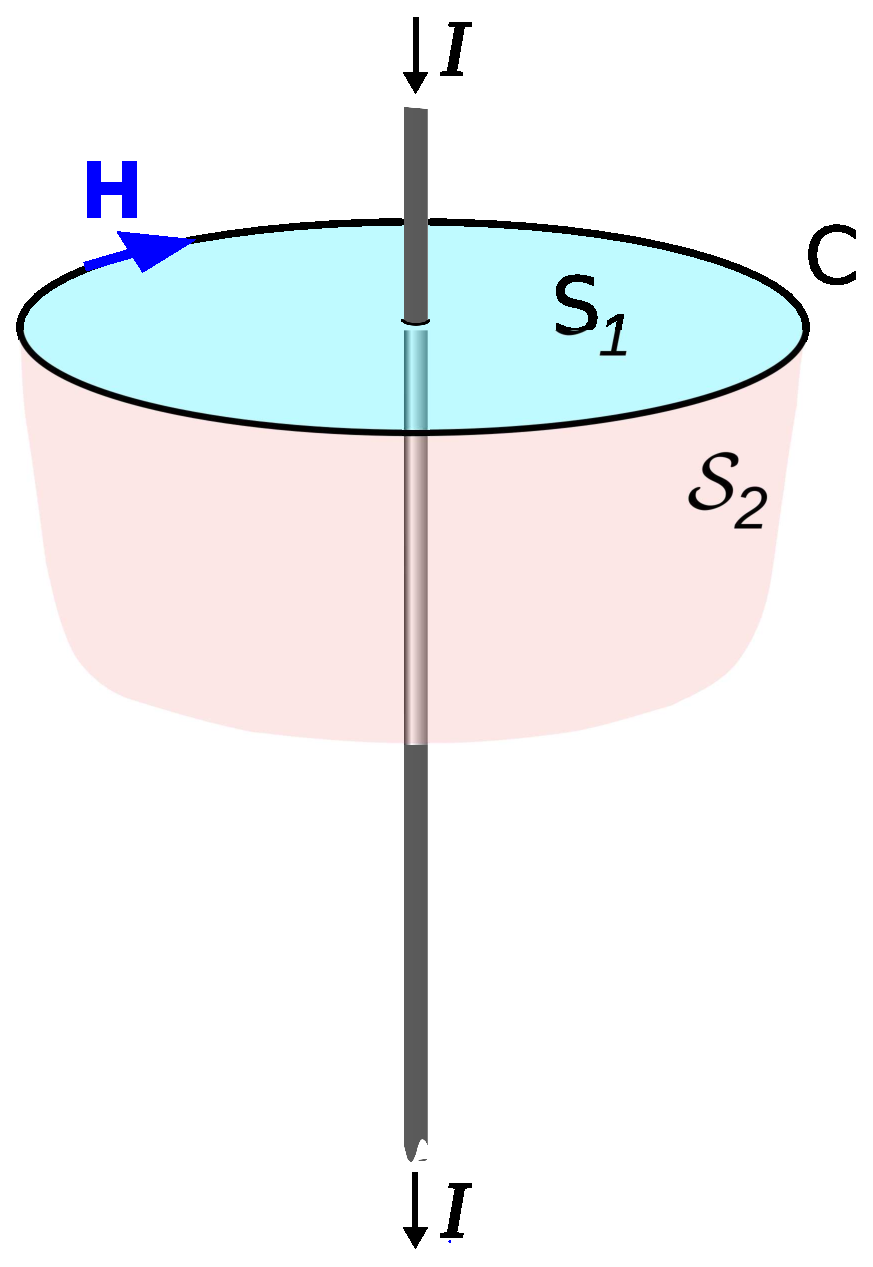
\includegraphics[width=2in]{modules/m0053_fDispCurrent1.eps}
% https://en.wikipedia.org/wiki/File:Displacement_current_in_capacitor.svg
}}{A vertical wire with current I moving down through it. The wire is surrounded by a light blue surface, S sub 1, which is bounded by a closed path, C. The magnetic field intensity, H, is represented by a blue arrow moving in a counterclockwise direction along C. Beneath the surface S sub 1 is a light pink surface, S sub 2, that is the same shape as S sub 1 but extends halfway down the wire, becoming slightly more narrow into a slightly conical shape. }
\end{center} 
\centerline{\scriptsize 
\hyperref[m0053_fDC_Credit]{C.\ Burks} (modified) 
} 
\caption{
\label{m0053_fDC}
Ampere's Law applied to a continuous line of current.
}
\end{figure}

Now consider the situation shown in Figure~\ref{m0053_fAC}, in which we have introduced a parallel-plate capacitor.
In the DC case, this situation is simple.  No current flows, so there is no magnetic field and Ampere's Law is trivially true. 
In the AC case, the current $I$ \emph{can} be non-zero,  but we must be clear about the physical origin of this current.  
What is happening is that for one half of a period, a source elsewhere in the circuit is moving positive charge to one side of the capacitor and negative charge to the other side.
For the other half-period, the source is exchanging the charge, so that negative charge appears on the previously positively-charged side and vice-versa.
Note that at no point is current flowing directly from one side of the capacitor to the other; instead, all current must flow through the circuit in order to arrive at the other plate.
Even though there is no current between the plates, there is current in the wire, and therefore there is also a magnetic field associated with that current.
%
\begin{figure}
\begin{center}
\pdftooltip{{  % note double braces
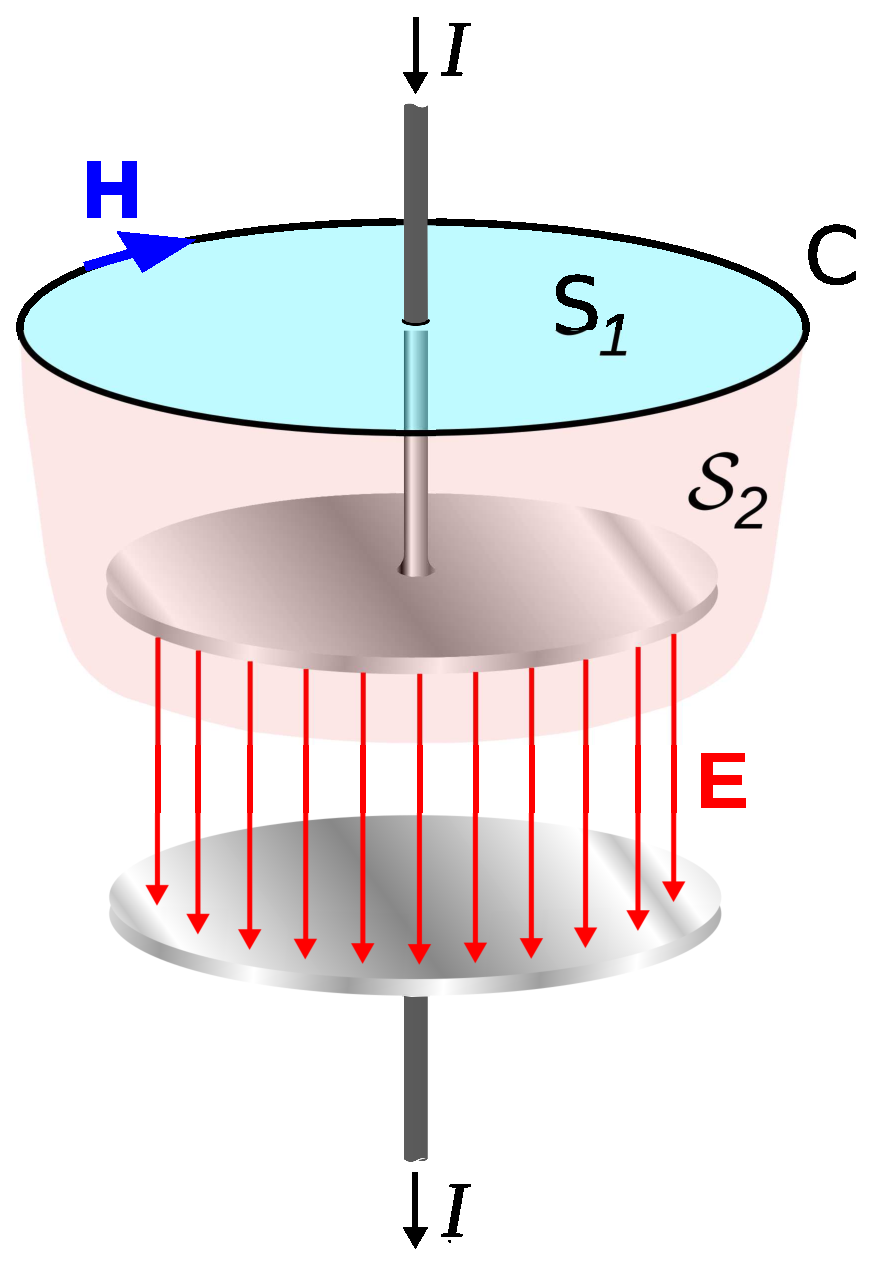
\includegraphics[width=2in]{modules/m0053_fDispCurrent2.eps}
% https://en.wikipedia.org/wiki/File:Displacement_current_in_capacitor.svg
}}{Similar to a previous figure, but features a parallel plate capacitor in the middle of the wire. In the space between the plates are red arrows pointed down in the direction of the electric field, labeled E.}
\end{center} 
\centerline{\scriptsize 
\hyperref[m0053_fAC_Credit]{C.\ Burks} (modified) 
} 
\caption{
\label{m0053_fAC}
Ampere's Law applied to a parallel plate capacitor.
}
\end{figure}

Now we are ready to shine a light on the problem.  
Recall that from Stokes' Theorem 
\index{Stokes' theorem}
(Section~\ref{m0051_Stokes_Theorem}), the line integral over ${\mathcal C}$ is mathematically equivalent to an integral over any open surface ${\mathcal S}$ that is bounded by ${\mathcal C}$.  
Two such surfaces are shown in Figure~\ref{m0053_fDC} and Figure~\ref{m0053_fAC}, indicated as ${\mathcal S}_1$ and ${\mathcal S}_2$.
In the wire-only scenario of Figure~\ref{m0053_fDC}, the choice of ${\mathcal S}$ clearly doesn't matter; any valid surface intersects current equal to $I$.
Similarly in the scenario of Figure~\ref{m0053_fAC}, everything seems fine if we choose ${\mathcal S}={\mathcal S}_1$.
If, on the other hand, we select ${\mathcal S}_2$ in the parallel-plate capacitor case, then we have a problem.  There is no current flowing through ${\mathcal S}_2$, so the right side of Equation~\ref{m0053_fACLI} is zero even though the left side is potentially non-zero.
So, it appears that something necessary for the time-varying case is missing from Equation~\ref{m0053_fACLI}.

To resolve the problem, we postulate an additional term in Ampere's Law that is non-zero in the above scenario.
Specifically, we propose:
%
\begin{equation}   
\oint_{\mathcal{C}}{ {\bf H} \cdot d{\bf l} } = I_c + I_d 
\end{equation}
%
where $I_c$ is the enclosed current (formerly identified as $I_{encl}$) and $I_d$ is the proposed new term.
If we are to accept this postulate, then here is a list of things we know about $I_d$:
%
\begin{itemize}
\item $I_d$ has units of current (A).
\item $I_d=0$ in the DC case and is potentially non-zero in the AC case.  This implies that $I_d$ is the time derivative of some other quantity.
\item $I_d$ must be somehow related to the electric field.
\end{itemize}
%
How do we know $I_d$ must be related to the electric field? This is because the Maxwell-Faraday Equation 
\index{Maxwell-Faraday equation}
(Section~\ref{m0050_Maxwell-Faraday_Equation}) tells us that spatial derivatives of ${\bf E}$ are related to time derivatives of ${\bf H}$; i.e., ${\bf E}$ and ${\bf H}$ are coupled in the time-varying (here, AC) case.  
This coupling between ${\bf E}$ and ${\bf H}$ must also be at work here, but we have not yet seen ${\bf E}$ play a role.  This is pretty strong evidence that $I_d$ depends on the electric field.

Without further ado, here's $I_d$:
%
\begin{equation}   
I_d = \int_{\mathcal{S}} { \frac{\partial {\bf D}}{\partial t} \cdot d{\bf s} }
\end{equation}
%
where ${\bf D}$ is the electric flux density (units of C/m$^2$) and is equal to $\epsilon{\bf E}$ as usual,
and $\mathcal{S}$ is the same open surface associated with $\mathcal{C}$ in Ampere's Law.
Note that this expression meets our expectations:
It is determined by the electric field, it is zero when the electric field is constant (i.e., not time varying), and has units of current.

The quantity $I_d$ is commonly known as \emph{displacement current}.
\index{displacement current}
It should be noted that this name is a bit misleading, since $I_d$ is not a current in the conventional sense.
Certainly, it is not a \emph{conduction} current -- conduction current is represented by $I_c$, and there is no current conducted through an ideal capacitor.
It is not unreasonable to think of $I_d$ as current in a more general sense, for the following reason.  At one instant, charge is distributed one way and at another, it is distributed in another way.  If you define current as a time variation in the charge distribution relative to $\mathcal{S}$ -- regardless of the path taken by the charge -- then $I_d$ is a current.
However, this distinction is a bit philosophical, so it may be less confusing to interpret ``displacement current'' instead as a separate electromagnetic quantity that just happens to have units of current.

Now we are able to write the general form of Ampere's Law that applies even when sources are time-varying.  Here it is:
%
\begin{equation}   
\boxed{
\oint_{\mathcal{C}}{ {\bf H} \cdot d{\bf l} } = I_c + \int_{\mathcal{S}} { \frac{\partial {\bf D}}{\partial t} \cdot d{\bf s} }
}
\label{m0053_eACLI} 
\end{equation}
%
As is the case in the Maxwell-Faraday Equation, most of the utility of Ampere's Law is unleashed when expressed in differential form.
To obtain this form the first step is to write $I_c$ as an integral of over $\mathcal{S}$; this is simply (see Section~\ref{m0101_Current_Distributions}):
%
\begin{equation}   
I_c = \int_{\mathcal{S}} {\bf J} \cdot d{\bf s} 
\end{equation}
%
where ${\bf J}$ is the volume current density (units of A/m$^2$).  So now we have
%
\begin{flalign}   
\oint_{\mathcal{C}}{ {\bf H} \cdot d{\bf l} } &= \int_{\mathcal{S}} {\bf J} \cdot d{\bf s}  + \int_{\mathcal{S}} { \frac{\partial {\bf D}}{\partial t} \cdot d{\bf s} } \nonumber \\
                                              &= \int_{\mathcal{S}} { \left({\bf J}+ \frac{\partial {\bf D}}{\partial t} \right) \cdot d{\bf s} } 
\end{flalign}
%
We can transform the left side of the above equation into a integral over $\mathcal{S}$ using Stokes' Theorem (Section~\ref{m0051_Stokes_Theorem}).
We obtain 
%
\begin{equation}   
\int_{\mathcal{S}} { \left( \nabla \times {\bf H} \right) \cdot d{\bf s}  }  = \int_{\mathcal{S}} { \left({\bf J}+ \frac{\partial {\bf D}}{\partial t} \right) \cdot d{\bf s} } 
\end{equation}
% 
The surface $\mathcal{S}$ on both sides is the same, and we have not constrained $\mathcal{S}$ in any way. $\mathcal{S}$ can be any mathematically-valid open surface anywhere in space, having any size and any orientation.
The only way the above expression can be universally true under these conditions is if the integrands on each side are equal at every point in space.
Therefore: 
%
\begin{equation}   
\boxed{
\nabla \times {\bf H} = {\bf J} + \frac{\partial}{\partial t}{\bf D}
}
\label{m0053_eACLD}
\end{equation}
%
which is Ampere's Law in differential form.

What does Equation~\ref{m0053_eACLD} mean? Recall that the curl of ${\bf H}$ is a way to describe the direction and rate of change of ${\bf H}$ with position.  Therefore, this equation constrains spatial derivatives of ${\bf H}$ to be simply related to ${\bf J}$ and the time derivative of ${\bf D}$ (displacement current).  Said plainly:

%ORB HIGHLIGHT
\begin{mdframed}[backgroundcolor=yellow!20,nobreak=true] 
The differential form of the general (time-varying) form of Ampere's Law (Equation~\ref{m0053_eACLD}) relates the change in the magnetic field with position to the change in the electric field with time, plus current.
\end{mdframed}

As is the case in the Maxwell-Faraday Equation (Section~\ref{m0050_Maxwell-Faraday_Equation}), we see that electric and magnetic fields become coupled at each point in space when sources are time-varying. 

%%%%%%%%%%%%%%%%%%%%%%%%%%%%%%%%%%%%%%

{\bf Additional Reading:}
\begin{itemize}
\item ``\href{https://en.wikipedia.org/wiki/Displacement_current}{Displacement Current}'' on Wikipedia.
\item ``\href{https://en.wikipedia.org/wiki/Ampere's_circuital_law}{Ampere's Circuital Law}'' on Wikipedia.
\item ``\href{https://en.wikipedia.org/wiki/Maxwell's_equations}{Maxwell's Equations}'' on Wikipedia.
\end{itemize}

\index{Ampere's law!general form|)}



%%%      \vfill\break
{\color{blue}\tiny[m0126]}    % This is text associated with the open textbook "Open Electromagnetics"
% See immediately below for author, date
% This work is licensed under the Creative Commons Attribution-ShareAlike 4.0 International License. (CC BY SA 4.0) 
% To view a copy of the license, visit http://creativecommons.org/licenses/by-sa/4.0/

%ORB TITLE Time-Varying Fields
%ORB AUTHOR 0        # S.W. Ellingson, Virginia Tech (ellingson@vt.edu)
%ORB DATE 20180701   # yyyymmdd
%ORB ABSTRACT End matter for chapter entitled "Time-Varying Fields"

\label{m0126_Ch_End_Matter_Time-Varying_Fields} % <-- Must match name of this file and module directory name.  Don't mess with this!

\onecolumn
\section*{Image Credits}

\begin{itemize}

\item[Fig.] \label{m0129_fLenzLaw_credit}
  \ref{m0129_fLenzLaw}:
  \copyright~Y.\ Qin, 
  \url{https://commons.wikimedia.org/wiki/File:M0003_fCoilBarMagnet.svg},\\ 
  CC BY 4.0 (\url{https://creativecommons.org/licenses/by/4.0/}), 
  modified from the original.

\item[Fig.] \label{m0129_fLLCoil_Credit}
  \ref{m0129_fLLCoil}:
  E.\ Bach, 
  {\footnotesize \url{https://commons.wikimedia.org/wiki/File:Faraday_emf_experiment.svg}},\\ 
  public domain via CC0 1.0 (\url{https://creativecommons.org/publicdomain/zero/1.0/deed.en}), 
  modified from the original.

\item[Fig.] \label{m0031_fTransformer3d_col3_Credit}
  \ref{m0031_fTransformer3d_col3}:
  \copyright~BillC, 
  {\footnotesize \url{https://commons.wikimedia.org/wiki/File:Transformer3d_col3.svg}},\\ 
  CC BY~SA 3.0 (\url{https://creativecommons.org/licenses/by-sa/3.0/}).
  Modified by author.

\item[Fig.] \label{m0032_fBalun_Credit}
  \ref{m0032_fBalun}:
  \copyright~SpinningSpark, 
  {\footnotesize \url{https://en.wikipedia.org/wiki/File:Transformer_balance.svg}},\\ 
  CC BY~SA 3.0 (\url{https://creativecommons.org/licenses/by-sa/3.0/}).
  Modified by author.

\item[Fig.] \label{m0053_fDC_Credit}
  \ref{m0053_fDC}:
  C.\ Burks, 
  {\footnotesize \url{https://en.wikipedia.org/wiki/File:Displacement_current_in_capacitor.svg}},\\ 
  public domain.
  Heavily modified by author.

\item[Fig.] \label{m0053_fAC_Credit}
  \ref{m0053_fAC}:
  C.\ Burks, 
  {\footnotesize \url{https://en.wikipedia.org/wiki/File:Displacement_current_in_capacitor.svg}},\\ 
  public domain.
  Heavily modified by author.

\end{itemize}

\twocolumn

  \chapter{Plane Waves in Lossless Media}
  \thispagestyle{fancy} % override footer in first page of chapter
  \fancyhf{}            % reset header and footer
  \fancyfoot[C]{\footnotesize \emph{Electromagnetics Vol~1}. ~\copyright~2018 S.W.\ Ellingson ~CC~BY~SA~4.0. ~\url{https://doi.org/10.21061/electromagnetics-vol-1}}
    \section{Maxwell's Equations in Differential Phasor Form}
{\color{blue}\tiny[m0042]}      % This is text associated with the open textbook "Open Electromagnetics"
% See immediately below for author, date
% This work is licensed under the Creative Commons Attribution-ShareAlike 4.0 International License. (CC BY SA 4.0) 
% To view a copy of the license, visit http://creativecommons.org/licenses/by-sa/4.0/

%ORB TITLE Maxwell's Equations in Differential Phasor Form
%ORB AUTHOR 0        # S.W. Ellingson, Virginia Tech (ellingson@vt.edu)
%ORB DATE 20180807   # yyyymmdd
%ORB ABSTRACT Maxwell's Equations in Differential Phasor Form 

\label{m0042_Phasor_Form_of_Maxwells_Equations_Differential} % <-- Must match name of this file and module directory name.  Don't mess with this!
\index{Maxwell's equations!differential phasor form|(}

In this section, we derive the phasor 
\index{phasor}
form of Maxwell's Equations from the general time-varying form of these equations.
Here we are interested exclusively in the differential (``point'') form of these equations. 
It is assumed that the reader is comfortable with phasor representation and its benefits; if not, a review of Section~\ref{m0033_Phasors} is recommended before attempting this section.

Maxwell's Equations in differential time-domain form are Gauss' Law (Section~\ref{m0045_Gauss_Law_Differential_Form_from_Integral_Form}):
%
\begin{equation}
\nabla\cdot{\bf D}=\rho_v
\label{m0042_eGL}
\end{equation}
%
the Maxwell-Faraday Equation (MFE; Section~\ref{m0050_Maxwell-Faraday_Equation}):
%
\begin{equation}
\nabla\times{\bf E}=-\frac{\partial}{\partial t}{\bf B}
\label{m0042_eMFE}
\end{equation}
%
Gauss' Law for Magnetism (GSM; Section~\ref{m0047_Gauss_Law_Magnetic_Differential_from_Integral}):
%
\begin{equation}
\nabla\cdot{\bf B}=0
\end{equation}
%
and Ampere's Law (Section~\ref{m0053_Displacement_Current_Amperes_Law}):
%
\begin{equation}
\nabla\times{\bf H}={\bf J} + \frac{\partial}{\partial t}{\bf D}
\end{equation}

We begin with Gauss's Law (Equation~\ref{m0042_eGL}).  We define $\widetilde{\bf D}$ and $\widetilde{\rho}_v$ as phasor quantities through the usual relationship:
 %
\begin{equation}   
{\bf D} = \mbox{Re} \left\{  \widetilde{\bf D} e^{j\omega t} \right\}
\end{equation}
%
and
%
\begin{equation}   
\rho_v = \mbox{Re} \left\{ \widetilde{\rho}_v e^{j\omega t} \right\}
\end{equation}
%
Substituting these expressions into Equation~\ref{m0042_eGL}:
 %
\begin{equation}   
\nabla \cdot \left[ \mbox{Re} \left\{  \widetilde{\bf D} e^{j\omega t} \right\} \right] = \mbox{Re} \left\{ \widetilde{\rho}_v e^{j\omega t} \right\}
\end{equation}
%
Divergence is a real-valued linear operator. Therefore, we may exchange the order of the ``Re'' and ``$\nabla\cdot$'' operations (this is ``Claim~2'' from Section~\ref{m0033_Phasors}):
 %
\begin{equation}   
\mbox{Re} \left\{  \nabla \cdot \left[ \widetilde{\bf D} e^{j\omega t}\right] \right\}  = \mbox{Re} \left\{ \widetilde{\rho}_v e^{j\omega t} \right\}
\end{equation}
%
Next, we note that the differentiation associated with the divergence operator is with respect to position and not with respect to time, so the order of operations may be further rearranged as follows:
  %
\begin{equation}   
\mbox{Re} \left\{  \left[ \nabla \cdot  \widetilde{\bf D} \right] e^{j\omega t} \right\}  = \mbox{Re} \left\{ \widetilde{\rho}_v e^{j\omega t} \right\}
\end{equation}
%
Finally, we note that the equality of the left and right sides of the above equation implies the equality of the associated phasors (this is ``Claim~1'' from Section~\ref{m0033_Phasors}); thus,
  %
\begin{equation}
\boxed{   
\nabla \cdot \widetilde{\bf D} = \widetilde{\rho}_v
}
\label{m0042_e1}
\end{equation}
%
In other words, the differential form of Gauss' Law for phasors is identical to the differential form of Gauss' Law for physical time-domain quantities. 

The same procedure applied to the MFE is only a little more complicated.
First, we establish the phasor representations of the electric and magnetic fields:
 %
\begin{equation}   
{\bf E} = \mbox{Re} \left\{  \widetilde{\bf E} e^{j\omega t} \right\}
\end{equation}
%
\begin{equation}   
{\bf B} = \mbox{Re} \left\{  \widetilde{\bf B} e^{j\omega t} \right\}
\end{equation}
%
After substitution into Equation~\ref{m0042_eMFE}:
 %
\begin{equation}   
\nabla \times \left[ \mbox{Re} \left\{  \widetilde{\bf E} e^{j\omega t} \right\} \right]   = 
-\frac{\partial}{\partial t} \left[ \mbox{Re} \left\{  \widetilde{\bf B} e^{j\omega t} \right\} \right]
\end{equation}
%
Both curl and time-differentiation are real-valued linear operations, so we are entitled to change the order of operations as follows:
%
\begin{equation}   
 \mbox{Re} \left\{  \nabla \times  \left[ \widetilde{\bf E} e^{j\omega t} \right] \right\}   = 
-\mbox{Re} \left\{ \frac{\partial}{\partial t} \left[  \widetilde{\bf B} e^{j\omega t} \right] \right\} 
\end{equation}
%
On the left, we note that the time dependence $e^{j\omega t}$ can be pulled out of the argument of the curl operator, since it does not depend on position: 
%
\begin{equation}   
 \mbox{Re} \left\{  \left[ \nabla \times  \widetilde{\bf E} \right] e^{j\omega t} \right\}   = 
-\mbox{Re} \left\{ \frac{\partial}{\partial t} \left[  \widetilde{\bf B} e^{j\omega t} \right] \right\} 
\end{equation}
%
On the right, we note that $\widetilde{\bf B}$ is constant with respect to time (because it is a phasor), so:
%
\begin{flalign}   
\mbox{Re} \left\{  \left[ \nabla \times  \widetilde{\bf E} \right] e^{j\omega t} \right\} &= -\mbox{Re} \left\{ \widetilde{\bf B} \frac{\partial}{\partial t} e^{j\omega t} \right\}  \nonumber \\
                                                                                          &= -\mbox{Re} \left\{ \widetilde{\bf B} j\omega e^{j\omega t} \right\} \nonumber \\
                                                                                          &= \mbox{Re} \left\{ \left[ -j\omega\widetilde{\bf B} \right] e^{j\omega t} \right\} 
\end{flalign}
%
And so we have found:
%
\begin{equation}   
\boxed{
\nabla \times  \widetilde{\bf E} = -j\omega\widetilde{\bf B}
}
\label{m0042_e2}
\end{equation}

Let's pause for a moment to consider the above result.  
In the general time-domain version of the MFE, we must take spatial derivatives of the electric field and time derivatives of the magnetic field.
In the phasor version of the MFE, the time derivative operator has been replaced with multiplication by $j\omega$.
This is a tremendous simplification since the equations now involve differentiation over position only.
Furthermore, no information is lost in this simplification -- for a reminder of why that is, see the discussion of Fourier Analysis at the end of Section~\ref{m0033_Phasors}.
Without this kind of simplification, much of what is now considered ``basic'' engineering electromagnetics would be intractable.

The procedure for conversion of the remaining two equations is very similar, yielding:
%
\begin{equation}   
\boxed{
\nabla \cdot \widetilde{\bf B} = 0
}
\label{m0042_e3}
\end{equation}
%
\begin{equation} 
\boxed{  
\nabla \times \widetilde{\bf H} = \widetilde{\bf J} + j\omega\widetilde{\bf D}
}
\label{m0042_e4}
\end{equation}
%
The details are left as an exercise for the reader.

%ORB HIGHLIGHT
\begin{mdframed}[backgroundcolor=yellow!20,nobreak=true] 
The differential form of Maxwell's Equations (Equations~\ref{m0042_e1}, \ref{m0042_e2}, \ref{m0042_e3}, and \ref{m0042_e4}) involve operations on the phasor representations of the physical quantities.
These equations have the advantage that differentiation with respect to time is replaced by multiplication by $j\omega$.
\end{mdframed}

\index{Maxwell's equations!differential phasor form|)}

      \vfill\break
    \section{Wave Equations for Source-Free and Lossless Regions}
{\color{blue}\tiny[m0036]}      % This is text associated with the open textbook "Open Electromagnetics"
% See immediately below for author, date
% This work is licensed under the Creative Commons Attribution-ShareAlike 4.0 International License. (CC BY SA 4.0) 
% To view a copy of the license, visit http://creativecommons.org/licenses/by-sa/4.0/

%ORB TITLE Wave Equations for Source-Free and Lossless Regions
%ORB AUTHOR 0        # S.W. Ellingson, Virginia Tech (ellingson@vt.edu)
%ORB DATE 20180807   # yyyymmdd
%ORB ABSTRACT Electromagnetic Wave Equations for source free regions, also assuming no loss (zero conductivity)

% original (long) title: "Electromagnetic Wave Equations for Source-Free and Lossless Regions"

\label{m0036_Wave_Equations_SourceFree_Lossless} % <-- Must match name of this file and module directory name.  Don't mess with this!
\index{wave equation!source-free lossless region|(}

Electromagnetic waves are solutions to a set of coupled differential simultaneous equations -- namely, Maxwell's Equations.
\index{Maxwell's equations}
The general solution to these equations includes constants whose values are determined by the applicable electromagnetic boundary conditions.
However, this direct approach can be difficult and is often not necessary.
In unbounded homogeneous regions that are ``source free'' (containing no charges or currents), a simpler approach is possible.
In this section, we reduce Maxwell's Equations to \emph{wave equations} that apply to the electric and magnetic fields in this simpler category of scenarios.
Before reading further, the reader should consider a review of Section~\ref{m0074_Fundamentals_of_Waves} (noting in particular Equation~\ref{m0074_eAcousticWaveEquation})
and Section~\ref{m0027_Wave_Equations_for_a_Transmission_Line} (wave equations for voltage and current on a transmission line).  
This section seeks to develop the analogous equations for electric and magnetic waves.

We can get the job done using the differential ``point'' phasor form of Maxwell's Equations, 
\index{Maxwell's equations!differential phasor form}
developed in Section~\ref{m0042_Phasor_Form_of_Maxwells_Equations_Differential}.  Here they are:
%
\begin{equation}
\nabla \cdot \widetilde{\bf D} = \widetilde{\rho}_v
\end{equation}
%
\begin{equation}   
\nabla \times  \widetilde{\bf E} = -j\omega\widetilde{\bf B}
\end{equation}
%
\begin{equation}   
\nabla \cdot \widetilde{\bf B} = 0
\end{equation}
%
\begin{equation} 
\nabla \times \widetilde{\bf H} = \widetilde{\bf J} + j\omega\widetilde{\bf D}
\end{equation}
%
In a source-free region, there is no net charge and no current, hence $\widetilde{\rho}_v=0$ and $\widetilde{\bf J}=0$ in the present analysis.  
The above equations become
%
\begin{equation}
\nabla \cdot \widetilde{\bf D} = 0
\end{equation}
%
\begin{equation}   
\nabla \times  \widetilde{\bf E} = -j\omega\widetilde{\bf B}
\end{equation}
%
%
\begin{equation}   
\nabla \cdot \widetilde{\bf B} = 0
\end{equation}
%
\begin{equation} 
\nabla \times \widetilde{\bf H} = +j\omega\widetilde{\bf D}
\end{equation}

Next, we recall that $\widetilde{\bf D}=\epsilon\widetilde{\bf E}$ and that $\epsilon$ is a real-valued constant for a medium that is homogeneous, 
\index{homogeneous (media)}
isotropic, 
\index{isotropic (media)}
and linear 
\index{linear (media)}
(Section~\ref{m0007_Properties_of_Materials}).
Similarly, $\widetilde{\bf B}=\mu\tilde{\bf H}$ and $\mu$ is a real-valued constant.
Thus, under these conditions, it is sufficient to consider \emph{either} $\widetilde{\bf D}$ or $\widetilde{\bf E}$ and \emph{either} $\widetilde{\bf B}$ or $\widetilde{\bf H}$.  The choice is arbitrary, but in engineering applications it is customary to use $\widetilde{\bf E}$ and $\widetilde{\bf H}$.
Eliminating the now-redundant quantities $\widetilde{\bf D}$ and $\widetilde{\bf B}$, the above equations become   
%
\begin{equation}
\nabla \cdot \widetilde{\bf E} = 0
\label{m0036_eGL3}
\end{equation}
%
\begin{equation}   
\nabla \times  \widetilde{\bf E} = -j\omega\mu\widetilde{\bf H}
\label{m0036_eMFE3}
\end{equation}
%
\begin{equation}
\nabla \cdot \widetilde{\bf H} = 0
\end{equation}
%
\begin{equation} 
\nabla \times \widetilde{\bf H} = +j\omega\epsilon\widetilde{\bf E}
\label{m0036_eAL3}
\end{equation}

It is important to note that requiring the region of interest to be source-free precludes the possibility of loss in the medium.
To see this, let's first be clear about what we mean by ``loss.''
For an electromagnetic wave, loss is observed as a reduction in the magnitude of the electric and magnetic field with increasing distance.
This reduction is due to the dissipation of power in the medium.
This occurs when the conductivity $\sigma$ is greater than zero because Ohm's Law for Electromagnetics 
\index{Ohm's law}
($\widetilde{\bf J}=\sigma\widetilde{\bf E}$; Section~\ref{m0010_Conductivity}) requires that power in the electric field be transferred into conduction current, and is thereby lost to the wave (Section~\ref{m0106_Power_Dissipation_in_Conducting_Media}).
When we required ${\bf J}$ to be zero above, we precluded this possibility; that is, we implicitly specified $\sigma=0$.
The fact that the constitutive parameters $\mu$ and $\epsilon$ appear in Equations~\ref{m0036_eGL3}--\ref{m0036_eAL3}, but $\sigma$ does not, is further evidence of this.

%ORB HIGHLIGHT
\begin{mdframed}[backgroundcolor=yellow!20,nobreak=true]
Equations~\ref{m0036_eGL3}--\ref{m0036_eAL3} are Maxwell's Equations 
\index{Maxwell's equations!source-free lossless region}
for a region comprised of isotropic, homogeneous, and source-free material.
Because there can be no conduction current in a source-free region, these equations apply only to material that is lossless (i.e., having negligible $\sigma$).
\end{mdframed}

Before moving on, one additional disclosure is appropriate. It turns out that there actually \emph{is} a way to use Equations~\ref{m0036_eGL3}--\ref{m0036_eAL3} for regions in which loss is significant.  This requires a redefinition of $\epsilon$ as a complex-valued quantity.  We shall not consider this technique in this section.  We mention this simply because one should be aware that if permittivity
\index{permittivity!complex-valued}
appears as a complex-valued quantity, then the imaginary part represents loss.

To derive the wave equations we begin with the MFE, Equation~\ref{m0036_eMFE3}.
Taking the curl of both sides of the equation we obtain
%
\begin{flalign}   
\nabla \times \left( \nabla \times  \widetilde{\bf E} \right) &= \nabla \times \left(  -j\omega\mu\widetilde{\bf H} \right)  \nonumber \\
                                                              &=   -j\omega\mu  \left(  \nabla \times \widetilde{\bf H} \right) 
\label{m0036_eWE1}
\end{flalign}
%
On the right we can eliminate $\nabla \times \widetilde{\bf H}$ using Equation~\ref{m0036_eAL3}:
%
\begin{flalign}  
-j\omega\mu  \left(  \nabla \times \widetilde{\bf H} \right) &= -j\omega\mu  \left( +j\omega\epsilon\widetilde{\bf E} \right) \nonumber \\
                                                             &= +\omega^2\mu\epsilon \widetilde{\bf E} 
\end{flalign}
%
On the left side of Equation~\ref{m0036_eWE1}, we apply the vector identity 
%
\begin{equation}
\nabla \times \nabla \times {\bf A} = \nabla\left(\nabla\cdot {\bf A}\right) -\nabla^2{\bf A}
\end{equation}
%
which in this case is
%
\begin{equation}
\nabla \times \nabla \times \widetilde{\bf E} = \nabla\left(\nabla\cdot \widetilde{\bf E}\right) -\nabla^2\widetilde{\bf E} 
\end{equation}
%
We may eliminate the first term on the right using Equation~\ref{m0036_eGL3}, yielding
%
\begin{equation}
\nabla \times \nabla \times \widetilde{\bf E} = -\nabla^2\widetilde{\bf E} 
\end{equation}
%
Substituting these results back into Equation~\ref{m0036_eWE1} and rearranging terms we have
%
\begin{equation}
\nabla^2\widetilde{\bf E} +\omega^2\mu\epsilon \widetilde{\bf E} = 0 
\label{m0036_eWEE1}
\end{equation}
%
This is the wave equation for $\widetilde{\bf E}$. 
Note that it is a homogeneous (in the mathematical sense of the word) differential equation, which is expected since we have derived it for a source-free region.

It is common to make the following definition
%
\begin{equation}
\boxed{
\beta \triangleq \omega\sqrt{\mu\epsilon} 
}
\label{m0036_eBetaDef}
\end{equation} 
%
so that Equation~\ref{m0036_eWEE1} may be written
%
\begin{equation}
\boxed{
\nabla^2\widetilde{\bf E} +\beta^2 \widetilde{\bf E} = 0 
}
\label{m0036_eWEE2}
\end{equation}
%
Why go the the trouble of defining $\beta$?
One reason is that $\beta$ conveniently captures the contribution of the frequency, permittivity, and permeability all in one constant.
Another reason is to emphasize the connection to the parameter $\beta$ appearing in transmission line theory (see Section~\ref{m0080_Wave_Propagation_on_a_Transmission_Line} for a reminder).  
It should be clear that $\beta$ is a \emph{phase propagation constant}, 
\index{propagation constant!phase}
having units of 1/m (or rad/m, if you prefer), and indicates the rate at which the phase of the propagating wave progresses with distance. 

The wave equation for $\widetilde{\bf H}$ is obtained using essentially the same procedure, which is left as an exercise for the reader. 
It should be clear from the duality 
\index{duality}
apparent in Equations~\ref{m0036_eGL3}-\ref{m0036_eAL3} that the result will be very similar. 
One finds:
%
\begin{equation}
\boxed{
\nabla^2\widetilde{\bf H} +\beta^2 \widetilde{\bf H} = 0 
}
\label{m0036_eWEH2}
\end{equation}

%ORB HIGHLIGHT
\begin{mdframed}[backgroundcolor=yellow!20,nobreak=true] 
Equations~\ref{m0036_eWEE2} and \ref{m0036_eWEH2} are the wave equations for $\widetilde{\bf E}$ and $\widetilde{\bf H}$, respectively, for a region comprised of isotropic, homogeneous, lossless, and source-free material.
\end{mdframed}

Looking ahead, note that $\widetilde{\bf E}$ and $\widetilde{\bf H}$ are solutions to the \emph{same} homogeneous differential equation.  Consequently, $\widetilde{\bf E}$ and $\widetilde{\bf H}$ cannot be different by more than a constant factor and a direction.
In fact, we can also determine something about the factor simply by examining the units involved:  
Since $\widetilde{\bf E}$ has units of V/m and $\widetilde{\bf H}$ has units of A/m, this factor will be expressible in units of the ratio of V/m to A/m, which is $\Omega$.
This indicates that the factor will be an impedance.
This factor is known as the \emph{wave impedance} 
\index{impedance!wave|see{wave impedance}}
\index{wave impedance}
and will be addressed in Section~\ref{m0039_Uniform_Plane_Waves_Characteristics}.
This impedance is analogous the characteristic impedance of a transmission line (Section~\ref{m0052_Characteristic_Impedance}).

%Solutions to the wave equation exist in a variety of forms, representing different types of waves. 
%These types are addressed in Section~\ref{m0142_Types_of_Waves}. 
%Here is a brief summary:
%%
%\begin{itemize}
%\item {\it Spherical}: Corresponding to waves appearing to radiate from (or to) a point,
%\item {\it Cylindrical}: Corresponding to waves appearing to radiate from (or to) a line,
%\item {\it Planar}: Corresponding to waves appearing to radiate from (or to) a plane (addressed beginning in Section~\ref{m0038_Uniform_Plane_Waves_Derivation}), 
%\item Other forms corresponding to other orthonormal coordinate systems, and
%\item Since superposition applies, linear combinations of the above types of waves are also solutions.
%\end{itemize}

%%%%%%%%%%%%%%%%%%%%%%%%%%%%%%%%%%%%%%%%%%%%%%%%%%%%%%%

{\bf Additional Reading:}
\begin{itemize}
\item ``\href{https://en.wikipedia.org/wiki/Wave_equation}{Wave Equation}'' on Wikipedia.
\item ``\href{https://en.wikipedia.org/wiki/Electromagnetic_wave_equation}{Electromagnetic Wave Equation}'' on Wikipedia.
\end{itemize}

\index{wave equation!source-free lossless region|)}




      \vfill\break
    \section{Types of Waves}
{\color{blue}\tiny[m0142]}      % This is text associated with the open textbook "Open Electromagnetics"
% See immediately below for author, date
% This work is licensed under the Creative Commons Attribution-ShareAlike 4.0 International License. (CC BY SA 4.0) 
% To view a copy of the license, visit http://creativecommons.org/licenses/by-sa/4.0/

%ORB TITLE Types of Waves  
%ORB AUTHOR 0       # S.W. Ellingson, Virginia Tech (ellingson@vt.edu)
%ORB DATE   20180807
%ORB ABSTRACT Introduction to planar, cylindrical, and spherical waves

\label{m0142_Types_of_Waves} % <-- Must match name of this file and module directory name.  Don't mess with this!

Solutions to the electromagnetic wave equations (Section~\ref{m0036_Wave_Equations_SourceFree_Lossless}) exist in a variety of forms, representing different types of waves. 
It is useful to identify three particular geometries for unguided waves. Each of these geometries is defined by the shape formed by surfaces of constant phase, which we refer to as \emph{phasefronts}.  
\index{phasefront}
(Keep in mind the analogy between electromagnetic waves and sound waves (described in Section~\ref{m0074_Fundamentals_of_Waves}), and note that sound waves also exhibit these geometries.)

A \emph{spherical wave} 
\index{waves!spherical}
has phasefronts that form concentric spheres, as shown in Figure~\ref{m0142_fSphericalPhasefront}.
Waves are well-modeled as spherical when the dimensions of the source of the wave are small relative to the scale at which the wave is observed.  
For example, the wave radiated by an antenna having dimensions of 10~cm, when observed in free space over a scale of 10~km, appears to have phasefronts that are very nearly spherical.
Note that the magnitude of the field on a phasefront of a spherical wave may vary significantly, but it is the shape of phasefronts that make it a spherical wave.
%
\begin{figure}
\begin{center}
\pdftooltip{{  % note double braces
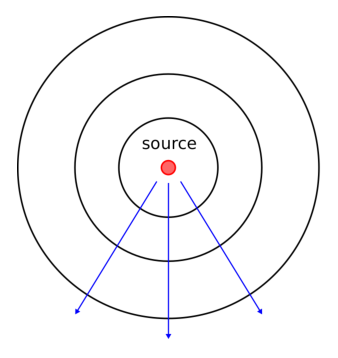
\includegraphics[width=2.5in]{modules/m0142_fSphericalPhasefront.eps}
% https://commons.wikimedia.org/wiki/File:M0142_fSphericalPhasefront.svg
}}{Three concentric circles, with a small red dot in the middle representing a source. From the source, three blue vectors extend down to the bottom left, directly below, and to the bottom right.}
\end{center} 
\centerline{\scriptsize 
\copyright~\hyperref[m0142_fSphericalPhasefront_Credit]{Y.\ Qin} 
\href{https://creativecommons.org/licenses/by/4.0/}{CC BY 4.0} 
} 
\caption{
\label{m0142_fSphericalPhasefront}
The phasefronts of a spherical wave form concentric spheres.
}
\end{figure}

A \emph{cylindrical wave} 
\index{waves!cylindrical}
exhibits phasefronts that form concentric cylinders, as shown in Figure~\ref{m0142_fCylindricalPhasefront}.
Said differently, the phasefronts of a cylindrical wave are circular in one dimension, and planar in the perpendicular direction.
A cylindrical wave is often a good description of the wave that emerges from a line-shaped source.
%
\begin{figure}
\begin{center}
\pdftooltip{{  % note double braces
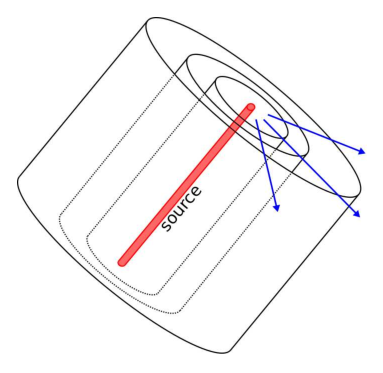
\includegraphics[width=2.5in]{modules/m0142_fCylindricalPhasefront.eps}
% https://commons.wikimedia.org/wiki/File:M0142_fCylindricalPhasefront.svg
}}{Three concentric cylinders, turned to the side so that the flat ends are pointing diagonally to the right. In the middle of the cylinders is a small red cylinder representing a source. From the source, three blue vectors extend along the face of the cylinders in the same directions as in a previous figure.}
\end{center} 
\centerline{\scriptsize 
\copyright~\hyperref[m0142_fCylindricalPhasefront_Credit]{Y.\ Qin} 
\href{https://creativecommons.org/licenses/by/4.0/}{CC BY 4.0} 
} 
\caption{
\label{m0142_fCylindricalPhasefront}
The phasefronts of a cylindrical wave form concentric cylinders.
}
\end{figure}

A \emph{plane wave} 
\index{waves!plane}
exhibits phasefronts that are planar, with planes that are parallel to each other as shown in Figure~\ref{m0142_fPlanarPhasefront}.
There are two conditions in which waves are well-modeled as plane waves.
First, some structures give rise to waves that appear to have planar phasefronts over a limited area; a good example is the wave radiated by a parabolic reflector, as shown in Figure~\ref{m0142_fPlaneWavesReflector}.
Second, all waves are well-modeled as plane waves when observed over a small region located sufficiently far from the source.
In particular, spherical waves are ``locally planar'' in the sense that they are well-modeled as planar when observed over a small portion of the spherical phasefront, as shown in Figure~\ref{m0142_fLocallyPlanar}.  
An analogy is that the Earth seems ``locally flat'' to an observer on the ground, even though it is clearly spherical to an observer in orbit.
The ``locally planar'' approximation is often employed because it is broadly applicable and simplifies analysis.
%
\begin{figure}
\begin{center}
\pdftooltip{{  % note double braces
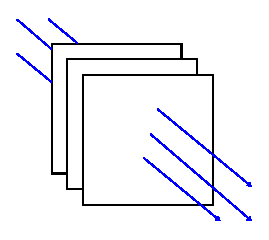
\includegraphics[width=2in]{modules/m0142_fPlanarPhasefront.eps}
% https://commons.wikimedia.org/wiki/File:M0142_fCylindricalPhasefront.svg
}}{Three square planes of the same size, laid on top of each other so that all are visible. Three equidistant blue vectors are shown behind the planes and extending from the middle of the front plane to show movement of the planes. }
\end{center} 
\centerline{\scriptsize 
\copyright~\hyperref[m0142_fPlanarPhasefront_Credit]{Y.\ Qin} 
\href{https://creativecommons.org/licenses/by/4.0/}{CC BY 4.0} 
} 
\caption{
\label{m0142_fPlanarPhasefront}
The phasefronts of a plane wave form parallel planes.
}
\end{figure}
%
\begin{figure}
\begin{center}
\pdftooltip{{  % note double braces
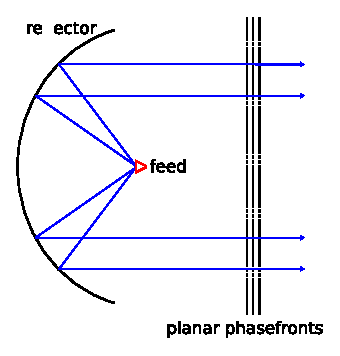
\includegraphics[width=2in]{modules/m0142_fPlaneWavesReflector.eps}
% https://commons.wikimedia.org/wiki/File:M0142_fPlaneWavesReflector.svg
}}{A parabolic reflector with open ends at slightly more than 90 degrees and less than 270 degrees to the left of three vertical dashed lines representing planar phasefronts. Between the reflector and the phasefronts is a small red triangle with the top pointed toward the phasefronts, representing feed. Four blue vectors extend from the left of the feed toward the reflector with the top two at slightly different angles and exactly mirroring the bottom two. After hitting the reflector, they follow a horizontal path right showing the direction of motion of the phasefronts.}
\end{center} 
\centerline{\scriptsize 
\copyright~\hyperref[m0142_fPlaneWavesReflector_Credit]{Y.\ Qin} 
\href{https://creativecommons.org/licenses/by/4.0/}{CC BY 4.0} 
} 
\caption{
\label{m0142_fPlaneWavesReflector}
Plane waves formed in the region in front of a parabolic reflector antenna.
}
\end{figure}
%
\begin{figure}
\begin{center}
\pdftooltip{{  % note double braces
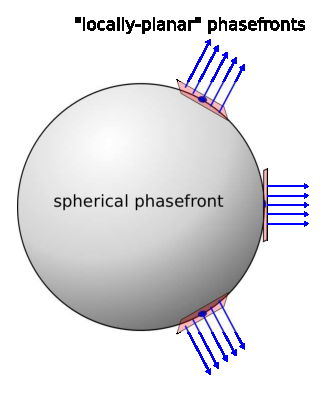
\includegraphics[width=2in]{modules/m0142_fLocallyPlanar.eps}
% https://commons.wikimedia.org/wiki/File:M0142_fLocallyPlanar.svg
}}{A three dimensional sphere, labeled "spherical phasefront". Tangent to the sphere are three red squares: one on the right, one on the upper right, and one on the lower right. From each of the red squares extends five blue vectors, pointing perpendicularly away from the sphere.}
\end{center} 
\centerline{\scriptsize 
\copyright~\hyperref[m0142_fLocallyPlanar_Credit]{Y.\ Qin} 
\href{https://creativecommons.org/licenses/by/4.0/}{CC BY 4.0} 
} 
\caption{
\label{m0142_fLocallyPlanar}
``Locally planar'' approximation of a spherical wave over a limited area.
}
\end{figure}

%ORB HIGHLIGHT
\begin{mdframed}[backgroundcolor=yellow!20,nobreak=true] 
Most waves are well-modeled as spherical, cylindrical, or plane waves.  
\end{mdframed}

%ORB HIGHLIGHT
\begin{mdframed}[backgroundcolor=yellow!20,nobreak=true] 
Plane waves (having planar phasefronts) are of particular importance due to wide applicability of the ``locally planar'' approximation. 
\end{mdframed}


      \vfill\break
    \section{Uniform Plane Waves: Derivation}
{\color{blue}\tiny[m0038]}      % This is text associated with the open textbook "Open Electromagnetics"
% See immediately below for author, date
% This work is licensed under the Creative Commons Attribution-ShareAlike 4.0 International License. (CC BY SA 4.0) 
% To view a copy of the license, visit http://creativecommons.org/licenses/by-sa/4.0/

%ORB TITLE Uniform Plane Waves: Derivation
%ORB AUTHOR 0        # S.W. Ellingson, Virginia Tech (ellingson@vt.edu)
%ORB DATE 20180807   # yyyymmdd
%ORB ABSTRACT Uniform Plane Waves: Derivation

\label{m0038_Uniform_Plane_Waves_Derivation} % <-- Must match name of this file and module directory name.  Don't mess with this!
\index{waves!plane|(}

Section~\ref{m0036_Wave_Equations_SourceFree_Lossless} showed how Maxwell's Equations could be reduced to a pair of phasor-domain ``wave equations,'' namely:
%
\begin{equation}
\nabla^2\widetilde{\bf E} +\beta^2 \widetilde{\bf E} = 0 
\label{m0038_eWEE2}
\end{equation}
%
\begin{equation}
\nabla^2\widetilde{\bf H} +\beta^2 \widetilde{\bf H} = 0 
\label{m0038_eWEH2}
\end{equation}
%
where $\beta=\omega\sqrt{\mu\epsilon}$, assuming unbounded homogeneous, isotropic, lossless, and source-free media.
In this section, we solve these equations for the special case of a uniform plane wave.
A uniform plane wave is one for which both $\widetilde{\bf E}$ and $\widetilde{\bf H}$ have constant magnitude and phase in a specified plane.  
Despite being a special case, the solution turns out to be broadly applicable, appearing as a common building block in many practical and theoretical problems in unguided propagation (as explained in Section~\ref{m0142_Types_of_Waves}), as well as in more than a few transmission line and waveguide problems.

To begin, let us assume that the plane over which $\widetilde{\bf E}$ and $\widetilde{\bf H}$ have constant magnitude and phase is a plane of constant $z$. 
% We will work the problem using the Cartesian coordinate system.
First, note that we may make this assumption with no loss of generality.
For example, we could alternatively select a plane of constant $y$, solve the problem, and then simply exchange variables to get a solution for planes of constant $z$ (or $x$).\footnote{By the way, this is a highly-recommended exercise for the student.}
%%% TODO Above
Furthermore, the solution for any planar orientation not corresponding to a plane of constant $x$, $y$, or $z$ may be similarly obtained by a rotation of coordinates, since the physics of the problem does not depend on the orientation of this plane -- if it does, then the medium is not isotropic!
 
We may express the constraint that the magnitude and phase of $\widetilde{\bf E}$ and $\widetilde{\bf H}$ are constant over a plane that is perpendicular to the $z$ axis as follows:
%
\begin{equation}
\frac{\partial}{\partial x} \widetilde{\bf E} = \frac{\partial}{\partial y} \widetilde{\bf E} 
= \frac{\partial}{\partial x} \widetilde{\bf H} = \frac{\partial}{\partial y} \widetilde{\bf H} 
= 0
\label{m0038_eWEPWP}
\end{equation}
%
Let us identify the Cartesian components of each of these fields as follows: 
%
\begin{flalign}
\widetilde{\bf E} &= \hat{\bf x}\widetilde{E}_x+\hat{\bf y}\widetilde{E}_y+\hat{\bf z}\widetilde{E}_z ~\mbox{, and} \\
\widetilde{\bf H} &= \hat{\bf x}\widetilde{H}_x+\hat{\bf y}\widetilde{H}_y+\hat{\bf z}\widetilde{H}_z
\end{flalign}
%
Now Equation~\ref{m0038_eWEPWP} may be interpreted in detail for $\widetilde{\bf E}$ as follows:
%
\begin{flalign}
\frac{\partial}{\partial x} \widetilde{E}_x = \frac{\partial}{\partial x} \widetilde{E}_y = \frac{\partial}{\partial x} \widetilde{E}_z &= 0 \label{m0038_eECxC} \\
\frac{\partial}{\partial y} \widetilde{E}_x = \frac{\partial}{\partial y} \widetilde{E}_y = \frac{\partial}{\partial y} \widetilde{E}_z &= 0 \label{m0038_eECyC}
\end{flalign}
%
and for $\widetilde{\bf H}$ as follows:
%
\begin{flalign}
\frac{\partial}{\partial x} \widetilde{H}_x = \frac{\partial}{\partial x} \widetilde{H}_y = \frac{\partial}{\partial x} \widetilde{H}_z &= 0 \\
\frac{\partial}{\partial y} \widetilde{H}_x = \frac{\partial}{\partial y} \widetilde{H}_y = \frac{\partial}{\partial y} \widetilde{H}_z &= 0 
\end{flalign}

The wave equation for $\widetilde{\bf E}$ (Equation~\ref{m0038_eWEE2}) written explicitly in Cartesian coordinates is
%
\begin{flalign}
\left[ \frac{\partial^2}{\partial x^2}  
+ \frac{\partial^2}{\partial y^2}  
+ \frac{\partial^2}{\partial z^2} \right]
&\left( \hat{\bf x}\widetilde{E}_x+\hat{\bf y}\widetilde{E}_y+\hat{\bf z}\widetilde{E}_z \right) \nonumber \\
+\beta^2 
&\left( \hat{\bf x}\widetilde{E}_x+\hat{\bf y}\widetilde{E}_y+\hat{\bf z}\widetilde{E}_z \right)
 = 0 
\end{flalign}
%  
Decomposing this equation into separate equations for each of the three coordinates, we obtain the following:
%
\begin{equation}
\left[ \frac{\partial^2}{\partial x^2} + \frac{\partial^2}{\partial y^2} + \frac{\partial^2}{\partial z^2} \right] \widetilde{E}_x + \beta^2 \widetilde{E}_x = 0 
\label{m0038_eECx}
\end{equation}
%
\begin{equation}
\left[ \frac{\partial^2}{\partial x^2} + \frac{\partial^2}{\partial y^2} + \frac{\partial^2}{\partial z^2} \right] \widetilde{E}_y + \beta^2 \widetilde{E}_y = 0 
\label{m0038_eECy}
\end{equation}
%
\begin{equation}
\left[ \frac{\partial^2}{\partial x^2} + \frac{\partial^2}{\partial y^2} + \frac{\partial^2}{\partial z^2} \right] \widetilde{E}_z + \beta^2 \widetilde{E}_z = 0 
\label{m0038_eECz}
\end{equation}
%%
Applying the constraints of Equations~\ref{m0038_eECxC} and \ref{m0038_eECyC}, we note that many of the terms in Equations~\ref{m0038_eECx}--\ref{m0038_eECz} are zero.  We are left with:
%
\begin{flalign}
\frac{\partial^2}{\partial z^2} \widetilde{E}_x + \beta^2 \widetilde{E}_x &= 0 \label{m0038_eWEPWE1} \\
\frac{\partial^2}{\partial z^2} \widetilde{E}_y + \beta^2 \widetilde{E}_y &= 0 \label{m0038_eWEPWE2} \\
\frac{\partial^2}{\partial z^2} \widetilde{E}_z + \beta^2 \widetilde{E}_z &= 0 \label{m0038_eWEPWE3}
%
\end{flalign}

Now we will show that Equation~\ref{m0038_eWEPWP} also implies that $\widetilde{E}_z$ must be zero.  
To show this, we use Ampere's Law for a source-free region (Section~\ref{m0036_Wave_Equations_SourceFree_Lossless}):
%
\begin{equation}
\nabla \times \widetilde{\bf H} = +j\omega\epsilon\widetilde{\bf E}
\end{equation}
%
and take the dot product with $\hat{\bf z}$ on both sides:
%
\begin{flalign}
\hat{\bf z} \cdot \left( \nabla \times \widetilde{\bf H} \right) &= +j\omega\epsilon \widetilde{E}_z \nonumber \\
\frac{\partial}{\partial y}\widetilde{H}_x - \frac{\partial}{\partial x}\widetilde{H}_y  &= +j\omega\epsilon \widetilde{E}_z
\label{m0038_eHxHyEz}
\end{flalign}
%
Again applying the constraints of Equation~\ref{m0038_eWEPWP}, the left side of Equation~\ref{m0038_eHxHyEz} must be zero; therefore, $\widetilde{E}_z=0$.  
The exact same procedure applied to $\widetilde{\bf H}$ (using the Maxwell-Faraday Equation; also given in Section~\ref{m0036_Wave_Equations_SourceFree_Lossless}) reveals that $\widetilde{H}_z$ is also zero.\footnote{Showing this is a highly-recommended exercise for the reader.} 
%%% TODO Above
Here is what we have found:
%
%ORB HIGHLIGHT
\begin{mdframed}[backgroundcolor=yellow!20,nobreak=true] 
If a wave is uniform over a plane, then the electric and magnetic field vectors must lie in this plane.
\end{mdframed}
%
This conclusion is a direct consequence of the fact that Maxwell's Equations require the electric field to be proportional to the curl of the magnetic field and vice-versa.  

The general solution to Equation~\ref{m0038_eWEPWE1} is:   
%
\begin{equation}
\widetilde{E}_x = E_{x0}^+ e^{-j\beta z} + E_{x0}^- e^{+j\beta z}
\label{m0038_ePWLM-Ex} 
\end{equation}
%
where $E_{x0}^+$ and $E_{x0}^-$ are complex-valued constants.  
The values of these constants are determined by boundary conditions -- possibly sources -- outside the region of interest.
Since in this section we are limiting our scope to source-free and homogeneous regions, we may for the moment consider the values of $E_{x0}^+$ and $E_{x0}^-$ to be arbitrary, since any values will satisfy the associated wave equation.\footnote{The reader is encouraged to confirm that these are solutions by substitution into the associated wave equation.}
%%% TODO Above

Similarly we have for $\widetilde{E}_y$:
%
\begin{equation}
\widetilde{E}_y = E_{y0}^+ e^{-j\beta z} + E_{y0}^- e^{+j\beta z}
\label{m0038_ePWLM-Ey} 
\end{equation}
%
where $E_{y0}^+$ and $E_{y0}^-$ are again arbitrary constants.  
Summarizing, we have found
%
\begin{equation}
\widetilde{\bf E} = \hat{\bf x}\widetilde{E}_x + \hat{\bf y}\widetilde{E}_y 
\end{equation}
%
where $\widetilde{E}_x$ and $\widetilde{E}_y$ are given by Equations~\ref{m0038_ePWLM-Ex} and \ref{m0038_ePWLM-Ey}, respectively.

Note that Equations~\ref{m0038_ePWLM-Ex} and \ref{m0038_ePWLM-Ey} are essentially the \emph{same} equations encountered in the study of waves in lossless transmission lines; for a reminder, see Section~\ref{m0027_Wave_Equations_for_a_Transmission_Line}.  Specifically, factors containing $e^{-j\beta z}$ describe propagation in the $+z$ direction, whereas factors containing $e^{+j\beta z}$ describe propagation in the $-z$ direction.  We conclude:
%
%ORB HIGHLIGHT
\begin{mdframed}[backgroundcolor=yellow!20,nobreak=true] 
If a wave is uniform over a plane, then possible directions of propagation are the two directions perpendicular to the plane. 
\end{mdframed}
%
Since we previously established that the electric and magnetic field vectors must lie in the plane, we also conclude:
%
%ORB HIGHLIGHT
\begin{mdframed}[backgroundcolor=yellow!20,nobreak=true] 
The direction of propagation is perpendicular to the electric and magnetic field vectors.
\end{mdframed}
%
This conclusion turns out to be generally true; i.e., it is not limited to uniform plane waves.  
Although we will not provide a rigorous proof of this, one way to see that this is true is to imagine that any type of wave can be interpreted as the sum (formally, a \emph{linear combination}) of uniform plane waves, so perpendicular orientation of the field vectors with respect to the direction of propagation is inescapable.  

The same procedure yields the uniform plane wave solution to the wave equation for $\widetilde{\bf H}$, which is
%
\begin{equation}
\widetilde{\bf H} = \hat{\bf x}\widetilde{H}_x + \hat{\bf y}\widetilde{H}_y 
\end{equation}
%
where
%
\begin{equation}
\widetilde{H}_x = H_{x0}^+ e^{-j\beta z} + H_{x0}^- e^{+j\beta z}
\label{m0038_ePWLM-Hx} 
\end{equation}
%
\begin{equation}
\widetilde{H}_y = H_{y0}^+ e^{-j\beta z} + H_{y0}^- e^{+j\beta z}
\label{m0038_ePWLM-Hy} 
\end{equation}
%
and where $H_{x0}^+$, $H_{x0}^-$, $H_{y0}^+$ and $H_{y0}^-$ are arbitrary constants.
Note that the solution is essentially the same as that for $\widetilde{\bf E}$, with the sole difference being that the arbitrary constants may apparently have different values. 

To this point, we have seen no particular relationship between the electric and magnetic fields, and it may appear that the electric and magnetic fields are independent of each other.
However, Maxwell's Equations -- specifically, the two curl equations -- make it clear that there must be a relationship between these fields.
Subsequently the arbitrary constants in the solutions for $\widetilde{\bf E}$ and $\widetilde{\bf H}$ must also be related.
In fact, there are two considerations here:
%
\begin{itemize}
\item The \emph{magnitude and phase} of $\widetilde{\bf E}$ must be related to the magnitude and phase of $\widetilde{\bf H}$.  
Since both fields are solutions to the same differential (wave) equation, they may differ by no more than a multiplicative constant.
Since the units of $\widetilde{\bf E}$ and $\widetilde{\bf H}$ are V/m and A/m respectively, this constant must be expressible in units of V/m divided by A/m; i.e., in units of $\Omega$, an impedance.
\item The \emph{direction} of $\widetilde{\bf E}$ must be related to direction of $\widetilde{\bf H}$.    
\end{itemize}
%
Let us now address these considerations.
Consider an electric field that points in one of the cardinal directions -- let's say $+\hat{\bf x}$ -- and make the definition $E_0 \triangleq E_{x0}^+$ for notational convenience.
Then the electric field intensity may be written as follows:
%
\begin{equation}
\widetilde{\bf E} = \hat{\bf x}E_0 e^{-j\beta z}
\label{m0038_eEx}
\end{equation}
%
Again, there is no loss of generality here since the coordinate system could be rotated in such a way that \emph{any} uniform plane could be described in this way. 

We may now determine $\widetilde{\bf H}$ from $\widetilde{\bf E}$ using the Maxwell-Faraday Equation 
\index{Maxwell-Faraday equation}
(Section~\ref{m0036_Wave_Equations_SourceFree_Lossless}):
%
\begin{equation}
\nabla \times  \widetilde{\bf E} = -j\omega\mu\widetilde{\bf H}
\end{equation}
%
Solving this equation for $\widetilde{\bf H}$, we find:
%
\begin{equation}
\widetilde{\bf H} = \frac{\nabla \times \widetilde{\bf E} }{-j\omega\mu} 
                  = \frac{\nabla \times \left[ \hat{\bf x}E_0 e^{-j\beta z} \right] }{-j\omega\mu}
\label{m0038_ePWLM-PWRH}
\end{equation}
%
Now let us apply the curl operator.
The complete expression for the curl operator in Cartesian coordinates is given in Section~\ref{m0139_Vector_Operators}.
Here let us consider one component at a time,
starting with the $\hat{\bf x}$ component:
%
\begin{equation}
\hat{\bf x}\cdot
\left( \nabla \times \widetilde{\bf E} \right) = 
\frac{\partial \widetilde{E}_z}{\partial y} - \frac{\partial \widetilde{E}_y}{\partial z} 
\end{equation}
%
Since $\widetilde{E}_y=\widetilde{E}_z=0$, the above expression is zero and subsequently $\widetilde{H}_x=0$.
Next, the $\hat{\bf y}$ component:
%
\begin{equation}
\hat{\bf y}\cdot
\left( \nabla \times \widetilde{\bf E} \right) = 
 \frac{\partial \widetilde{E}_x}{\partial z} - \frac{\partial \widetilde{E}_z}{\partial x} 
\end{equation}
%
Here $\widetilde{E}_z=0$, so we have simply
%
\begin{equation}
%\widetilde{H}_y = 
\hat{\bf y}\cdot
\left( \nabla \times \widetilde{\bf E} \right) = \frac{ \partial \widetilde{E}_x}{\partial z}
\end{equation}
%
It is not necessary to repeat this procedure for $\widetilde{H}_z$, since we know in advance that $\widetilde{\bf H}$ must be perpendicular to the direction of propagation and subsequently $\widetilde{H}_z=0$.
Returning to Equation~\ref{m0038_ePWLM-PWRH}, we obtain:
%
\begin{flalign}
\widetilde{\bf H} &= \hat{\bf y} \frac{ 1 }{-j\omega\mu} \frac{ \partial }{\partial z} \widetilde{E}_x \nonumber \\
                  &= \hat{\bf y} \frac{ 1 }{-j\omega\mu} \frac{ \partial}{\partial z} \left( E_0 e^{-j\beta z} \right) \nonumber \\
                  &= \hat{\bf y} \frac{ 1 }{-j\omega\mu} \left( -j\beta E_0 e^{-j\beta z} \right) \nonumber \\
                  &= \hat{\bf y} \frac{ \beta }{\omega\mu} E_0 e^{-j\beta z} 
\label{m0038_eHy}
\end{flalign}

Note that $\widetilde{\bf H}$ points in the $+\hat{\bf y}$ direction.
So, as expected, both $\widetilde{\bf E}$ and $\widetilde{\bf H}$ are perpendicular to the direction of propagation.
However, we have now found a more specific relationship: $\widetilde{\bf E}$ and $\widetilde{\bf H}$ are perpendicular \emph{to each other}.
Just as $\hat{\bf x} \times \hat{\bf y} = \hat{\bf z}$, we see that $\widetilde{\bf E} \times \widetilde{\bf H}$ points in the direction of propagation.
This is illustrated in Figure~\ref{m0038_fEHk}.
Summarizing:
%
%ORB HIGHLIGHT
\begin{mdframed}[backgroundcolor=yellow!20,nobreak=true] 
$\widetilde{\bf E}$, $\widetilde{\bf H}$, and the direction of propagation $\widetilde{\bf E} \times \widetilde{\bf H}$ are mutually perpendicular.
\end{mdframed}
%
\begin{figure}
\begin{center}
\pdftooltip{{  % note double braces
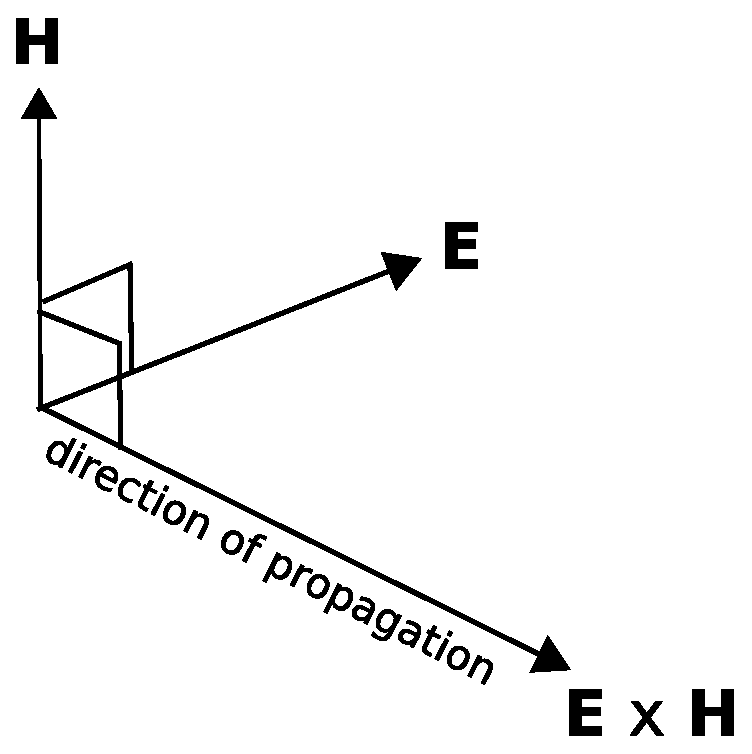
\includegraphics[width=2in]{modules/m0038_fEHk.eps}
% URL goes here
}}{A Cartesian plane with H, E, and E cross H axes. The H-axis points vertically. The E-axis and E cross H axes are perpendicular to the H-axis and each other. They are connected by the origin. The E cross H axis is labeled "direction of propagation".}
\end{center} 
%\centerline{\scriptsize 
%\copyright~\hyperref[m0039_Onde_electromagnetique_Credit]{E.\ Boutet} (Modified) 
%\href{https://creativecommons.org/licenses/by-sa/3.0/}{CC BY-SA 3.0} 
%} 
\caption{
\label{m0038_fEHk}
Relationship between the electric field direction, magnetic field direction, and direction of propagation.
}
\end{figure}
%

Now let us resolve the question of the factor relating $\widetilde{\bf E}$ and $\widetilde{\bf H}$.
The factor is now seen to be $\beta/\omega\mu$ in Equation~\ref{m0038_eHy}, which can be simplified as follows: 
%
\begin{equation}
\frac{\beta}{\omega\mu} = \frac{\omega\sqrt{\mu\epsilon}}{\omega\mu} = \frac{1}{\sqrt{\mu/\epsilon}}
\end{equation}
%
The factor $\sqrt{\mu/\epsilon}$ appearing above has units of $\Omega$ is known variously as the \emph{wave impedance} 
\index{wave impedance}
or the \emph{intrinsic impedance of the medium}.
Assigning this quantity the symbol ``$\eta$,'' we have:
%
\begin{equation}
\boxed{
\eta \triangleq \frac{\widetilde{E}_x}{\widetilde{H}_y} = \sqrt{\frac{\mu}{\epsilon}}
}
\label{m0038_eEta}
\end{equation}
%
%ORB HIGHLIGHT
\begin{mdframed}[backgroundcolor=yellow!20,nobreak=true] 
The ratio of the electric field intensity to the magnetic field intensity is the wave impedance $\eta$ (Equation~\ref{m0038_eEta}; units of $\Omega$).  
In lossless media, $\eta$ is determined by the ratio of permeability of the medium to the permittivity of the medium. 
\end{mdframed}
%
The wave impedance in free space, assigned the symbol $\eta_0$, is
%
\begin{equation}
\eta_0 \triangleq \sqrt{\frac{\mu_0}{\epsilon_0}} \cong 377~\Omega. 
\end{equation}

Wrapping up our solution, we find that if $\widetilde{\bf E}$ is as given by Equation~\ref{m0038_eEx}, then
%
\begin{equation}
\widetilde{\bf H} = \hat{\bf y}\frac{E_0}{\eta} e^{-j\beta z}
\end{equation}

%%% TODO Example: Change orientation of E, direction of propagation, what is new H; then reference m0039 (Plane Wave Relationship)

\index{waves!plane|)}

      \vfill\break
    \section{Uniform Plane Waves: Characteristics}
{\color{blue}\tiny[m0039]}      % This is text associated with the open textbook "Open Electromagnetics"
% See immediately below for author, date
% This work is licensed under the Creative Commons Attribution-ShareAlike 4.0 International License. (CC BY SA 4.0) 
% To view a copy of the license, visit http://creativecommons.org/licenses/by-sa/4.0/

%ORB TITLE Uniform Plane Waves: Characteristics
%ORB AUTHOR 0        # S.W. Ellingson, Virginia Tech (ellingson@vt.edu)
%ORB DATE 20180807   # yyyymmdd
%ORB ABSTRACT Uniform Plane Waves: Characteristics

\label{m0039_Uniform_Plane_Waves_Characteristics} % <-- Must match name of this file and module directory name.  Don't mess with this!
\index{waves!plane|(}

In Section~\ref{m0038_Uniform_Plane_Waves_Derivation}, expressions for the electric and magnetic fields are determined for a uniform plane wave in lossless media.
If the planar phasefront
\index{phasefront}
is perpendicular to the $z$ axis, then waves may propagate in either the $+\hat{\bf z}$ direction of the $-\hat{\bf z}$ direction.  
If we consider only the former, and select $\widetilde{\bf E}$ to point in the $+\hat{\bf x}$ direction, then we find
%
\begin{equation}
\widetilde{\bf E} = +\hat{\bf x}E_0 e^{-j\beta z}
\label{m0039_eE}
\end{equation}
%
\begin{equation}
\widetilde{\bf H} = +\hat{\bf y}\frac{E_0}{\eta} e^{-j\beta z}
\label{m0039_eH}
\end{equation}
%
where 
$\beta=\omega\sqrt{\mu\epsilon}$ is the phase propagation constant,
$\eta=\sqrt{\mu/\epsilon}$ is the wave impedance, and
$E_0$ is a complex-valued constant associated with the magnitude and phase of the source.
This result is in fact completely general for uniform plane waves, since any other possibility may be obtained by simply rotating coordinates.  
In fact, this is pretty easy because (as determined in Section~\ref{m0038_Uniform_Plane_Waves_Derivation}) $\widetilde{\bf E}$, $\widetilde{\bf H}$, and the direction of propagation are mutually perpendicular, with the direction of propagation pointing in the same direction as $\widetilde{\bf E} \times \widetilde{\bf H}$.

In this section, we identify some important characteristics of uniform plane waves, including wavelength and phase velocity.  
Chances are that much of what appears here will be familiar to the reader; if not, a quick review of Sections~\ref{m0074_Fundamentals_of_Waves} (``Fundamentals of Waves'') and \ref{m0080_Wave_Propagation_on_a_Transmission_Line} (``Wave Propagation on a Transmission Line'') are recommended.

First, recall that $\widetilde{\bf E}$ and $\widetilde{\bf H}$ are phasors 
\index{phasor}
representing physical (real-valued) fields and are \emph{not} the field values themselves.  
The actual, physical electric field intensity is
%
\begin{flalign}
{\bf E} &= \mbox{Re} \left\{ \widetilde{\bf E} e^{j\omega t} \right\} \label{m0039_eEP} \\
        &= \mbox{Re} \left\{ \hat{\bf x} E_0 e^{-j\beta z} e^{j\omega t} \right\} \nonumber \\
        &= \hat{\bf x}\left| E_0 \right| \cos\left(\omega t - \beta z + \psi \right) \nonumber
\end{flalign}
%
where $\psi$ is the phase of $E_0$.  Similarly:
%
\begin{equation}
{\bf H} = \hat{\bf y}\frac{\left| E_0 \right|}{\eta} \cos\left(\omega t - \beta z + \psi \right)
\label{m0039_eH2}
\end{equation}
%
This result is illustrated in Figure~\ref{m0039_fPWR}.
Note that both ${\bf E}$ and ${\bf H}$ (as well as their phasor representations) have the same phase and have the same frequency and position dependence $\cos\left(\omega t - \beta z + \psi \right)$.  
Since $\beta$ is a real-valued constant for lossless media, {\it only} the phase, and not the magnitude, varies with $z$.
If $\omega \to 0$, then $\beta \to 0$ and the fields no longer depend on $z$; in this case, the field is not propagating.   
For $\omega > 0$, $\cos\left(\omega t - \beta z + \psi \right)$ is periodic in $z$; specifically, it has the same value each time $z$ increases or decreases by $2\pi/\beta$.  
This is, by definition, the wavelength 
\index{wavelength}
$\lambda$: 
%
\begin{equation}
\lambda \triangleq \frac{2\pi}{\beta}
\end{equation}
%
\begin{figure}
\begin{center}
\pdftooltip{{  % note double braces
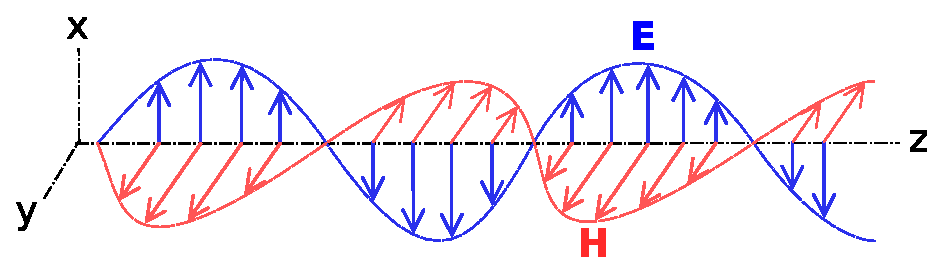
\includegraphics[width=\columnwidth]{modules/m0039_Onde_electromagnetique.eps}
% https://en.wikipedia.org/wiki/File:Onde_electromagnetique.svg
}}{Plotted on a three dimensional xyz coordinate system sits two sinusoidal waves perpendicular to one another. In the y-z plane sits the sinusoidal magnetic field wave. In the x-z plane sits the sinusoidal electric field wave. Each wave has vectors pointing from the axis to the wave.}
\end{center} 
\centerline{\scriptsize 
\copyright~\hyperref[m0039_Onde_electromagnetique_Credit]{E.\ Boutet} (Modified) 
\href{https://creativecommons.org/licenses/by-sa/3.0/}{CC BY~SA 3.0} 
} 
\caption{
\label{m0039_fPWR}
Relationship between the electric field direction, magnetic field direction, and direction of propagation (here, $+\hat{\bf z}$).
}
\end{figure}

If we observe this wave at some fixed point (i.e., hold $z$ constant), we find that the electric and magnetic fields are also periodic in time; specifically, they have the same value each time $t$ increases by $2\pi/\omega$.  We may characterize the speed at which the wave travels by comparing 
the distance required to experience $2\pi$ of phase rotation at a fixed time, which is $1/\beta$; to
the time it takes to experience $2\pi$ of phase rotation at a fixed location, which is $1/\omega$.  This is known as the {\it phase velocity}\footnote{We acknowledge that this is a misnomer, since velocity is properly defined as speed in a \emph{specified} direction, and $v_p$ by itself does not specify direction. In fact, the phase velocity in this case is properly said to be $+\hat{\bf z}v_p$.  Nevertheless, we adopt the prevailing terminology.} $v_p$:
\index{phase velocity}
%
\begin{equation}
v_p \triangleq \frac{1/\beta}{1/\omega} = \frac{\omega}{\beta} 
\end{equation}
%
Note that $v_p$ has the units expected from its definition, namely (rad/s)/(rad/m) $=$ m/s. If we make the substitution $\beta=\omega\sqrt{\mu\epsilon}$, we find
%
\begin{equation}
v_p = \frac{\omega}{\omega\sqrt{\mu\epsilon}} = \frac{1}{\sqrt{\mu\epsilon}}
\end{equation}
%
Note that $v_p$, like the wave impedance $\eta$, depends only on material properties.  
For example, the phase velocity of an electromagnetic wave in free space, given the special symbol $c$, is
%
\begin{equation}
c \triangleq \left. v_p \right|_{\mu=\mu_0, \epsilon=\epsilon_0} = \frac{1}{\sqrt{\mu_0\epsilon_0 }} \cong 3.00 \times 10^8~\mbox{m/s}
\end{equation}
%
This constant is commonly referred to as the \emph{speed of light}, 
\index{speed of light}
but in fact it is the phase velocity of an electromagnetic field at \emph{any} frequency (not just optical frequencies) in free space.  
Since the permittivity $\epsilon$ and permeability $\mu$ of any material is greater than that of a vacuum, $v_p$ in any material is less than the phase velocity in free space.
Summarizing:
%
%ORB HIGHLIGHT
\begin{mdframed}[backgroundcolor=yellow!20,nobreak=true] 
Phase velocity is the speed at which any point of constant phase appears to travel along the direction of propagation.
\end{mdframed}
%
%ORB HIGHLIGHT
\begin{mdframed}[backgroundcolor=yellow!20,nobreak=true] 
Phase velocity is maximum ($=c$) in free space, and slower by a factor of $1/\sqrt{\mu_r\epsilon_r}$ in any other lossless medium. 
\end{mdframed}

Finally, we note the following relationship between frequency $f$, wavelength, and phase velocity:
%
\begin{equation}
\lambda = \frac{2\pi}{\beta} 
= \frac{2\pi}{\omega / v_p}
= \frac{2\pi}{2\pi f / v_p}
= \frac{v_p}{f}
\end{equation}
%
Thus, given any two of the parameters $f$, $\lambda$, and $v_p$, we may solve for the remaining quantity.  
Also note that as a consequence of the inverse-proportional relationship between $\lambda$ and $v_p$, we find:
%
%ORB HIGHLIGHT
\begin{mdframed}[backgroundcolor=yellow!20,nobreak=true] 
At a given frequency, the wavelength in any material is shorter than the wavelength in free space.
\end{mdframed}

%%%%%%%%%%%%%%%%%%%%%%%%%%%%%%%%%%%%%%%%%%%%%%%
%ORB EXAMPLE
~\\ \begin{example} 
\begin{mdframed}[backgroundcolor=brown!20,linecolor=brown!20]\raggedright
Wave propagation in a lossless dielectric.
\index{dielectric (material)}
\\~\\
Polyethylene is a low-loss dielectric having $\epsilon_r \cong 2.3$.
What is the phase velocity in polyethylene?
What is wavelength in polyethylene?
The frequency of interest is 1~GHz.


{\bf Solution.}
Low-loss dielectrics exhibit $\mu_r \cong 1$ and $\sigma\approx 0$.
Therefore the phase velocity is
%
\begin{equation}
v_p = \frac{1}{\sqrt{\mu_0\epsilon_r\epsilon_0 }} = \frac{c}{\sqrt{\epsilon_r}} \cong 1.98 \times 10^8~\mbox{m/s}
\end{equation}
%
i.e., very nearly two-thirds of the speed of light in free space.
The wavelength at 1~GHz is
%
\begin{equation}
\lambda = \frac{v_p}{f} \cong 19.8~\mbox{cm}
\end{equation}
%
Again, about two-thirds of a wavelength at the same frequency in free space.

\end{mdframed}
% note figures will need to go between "\end{mdframed}" and "\end{example}"
\end{example}
%%%%%%%%%%%%%%%%%%%%%%%%%%%%%%%%%%%%%%%%%%%%%%%


Returning to polarization and magnitude, it is useful to note that Equation~\ref{m0039_eH2} could be written in terms of {\bf E} as follows:
%
\begin{equation}
{\bf H} = \frac{1}{\eta} \hat{\bf z} \times {\bf E} 
\end{equation}
%
i.e., ${\bf H}$ is perpendicular to both the direction of propagation (here, $+\hat{\bf z}$) and ${\bf E}$, with magnitude that is different from ${\bf E}$ by the wave impedance $\eta$.
%
This simple expression is very useful for quickly determining ${\bf H}$ given ${\bf E}$ when the direction of propagation is known.  
In fact, it is so useful that it commonly explicitly generalized as follows:
%
\begin{equation}
\boxed{
{\bf H} = \frac{1}{\eta} \hat{\bf k} \times {\bf E} 
}
\label{m0039_ePWRH}
\end{equation}
%
where $\hat{\bf k}$ (here, $+\hat{\bf z}$) is the direction of propagation.
Similarly, given ${\bf H}$, $\hat{\bf k}$, and $\eta$, we may find ${\bf E}$ using
%
\begin{equation}
\boxed{
{\bf E} = -\eta \hat{\bf k} \times {\bf H} 
}
\label{m0039_ePWRE}
\end{equation}
%
These spatial relationships can be readily verified using Figure~\ref{m0039_fPWR}.
%
%ORB HIGHLIGHT
\begin{mdframed}[backgroundcolor=yellow!20,nobreak=true] 
Equations~\ref{m0039_ePWRH} and \ref{m0039_ePWRE} are known as the \emph{plane wave relationships}.
\index{plane wave relationships}
\end{mdframed}
%
The plane wave relationships apply equally well to the phasor representations of ${\bf E}$ and ${\bf H}$; i.e.,
\begin{flalign}
\widetilde{\bf E} &= -\eta \hat{\bf k} \times \widetilde{\bf H} \\
\widetilde{\bf H} &= \frac{1}{\eta} \hat{\bf k} \times \widetilde{\bf E} 
\end{flalign}
%
These equations can be readily verified by applying the definition of the associated phasors (e.g., Equation~\ref{m0039_eEP}).
It also turns out that these relationships apply at each point in space, even if the waves are not planar, uniform, or in lossless media.

%%%%%%%%%%%%%%%%%%%%%%%%%%%%%%%%%%%%%%%%%%%%%%%
%ORB EXAMPLE
~\\ \begin{example} 
\begin{mdframed}[backgroundcolor=brown!20,linecolor=brown!20]\raggedright
Analysis of a radially-directed plane wave.
\\~\\
Consider the scenario illustrated in Figure~\ref{m0039_fEx1}.
Here a uniform plane wave having frequency $f=3$~GHz is propagating along a path of constant $\phi$, where is $\phi$ is known but not specified.  
The phase of the electric field is $\pi/2$~radians at $\rho=0$ (the origin) and $t=0$.
The material is an effectively unbounded region of free space.  
The electric field is oriented in the $+\hat{\bf z}$ direction and has peak magnitude of 1~mV/m.  
Find 
(a) the electric field intensity in phasor representation, 
(b) the magnetic field intensity in phasor representation, and 
(c) the actual, physical electric field along the radial path. 

{\bf Solution}: 
First, realize that this ``radially-directed'' plane wave is in fact a plane wave, and not a cylindrical wave.
It may well we be that if we ``zoom out'' far enough, we are able to perceive a cylindrical wave (for more on this idea, see Section~\ref{m0142_Types_of_Waves}), or it might simply be that wave is \emph{exactly} planar, and cylindrical coordinates just happen to be a convenient coordinate system for this application.
In either case, the direction of propagation $\hat{\bf k}=+\hat{\bf \rho}$ and the solution to this example will be the same.
 
Here's the phasor representation for the electric field intensity of a uniform plane wave in a lossless medium, analogous to Equation~\ref{m0039_eE}:
%
\begin{equation}
\widetilde{\bf E} = +\hat{\bf z}E_0 e^{-j\beta \rho} 
\end{equation}
%
From the problem statement, $\left|E_0\right| = 1$~mV/m.
Also from the problem statement, the phase of $E_0$ is $\pi/2$ radians; in fact, we could just write $E_0 = +j\left|E_0\right|$.
Thus, the answer to (a) is 
%
\begin{equation}
\widetilde{\bf E} = +\hat{\bf z}j\left|E_0\right| e^{-j\beta\rho}
\end{equation}
%
where the propagation constant $\beta = \omega\sqrt{\mu\epsilon} = 2\pi f \sqrt{\mu_0 \epsilon_0} \cong 62.9$~rad/m.  

The answer to (b) is easiest to obtain from the plane wave relationship:
%
\begin{flalign}
\widetilde{\bf H} &= \frac{1}{\eta} \hat{\bf k} \times {\bf E} \nonumber \\
                  &= \frac{1}{\eta} \hat{\bf \rho} \times \left( +\hat{\bf z}j\left|E_0\right| e^{-j\beta\rho} \right) \nonumber \\
                  &=-\hat{\bf \phi} \frac{j\left|E_0\right|}{\eta}  e^{-j\beta\rho} 
\end{flalign}
%
where $\eta$ here is $\sqrt{\mu_0/\epsilon_0} \cong 377~\Omega$. Thus, the answer to part (b) is
%
\begin{equation}
\widetilde{\bf H} = -\hat{\bf \phi}jH_0 e^{-j\beta\rho}
\end{equation}
%
where $H_0 \cong 2.65~\mu$A/m.
At this point you should check vector directions: $\widetilde{\bf E} \times \widetilde{\bf H}$ should point in the direction of propagation $+\hat{\bf \rho}$.
Here we find $\hat{\bf z} \times \left(-\hat{\bf \phi}\right) = +\hat{\bf \rho}$, as expected.

The answer to (c) is obtained by applying the defining relationship for phasors to the answer to part (a):
%
\begin{flalign}
{\bf E} &= \mbox{Re} \left\{ \widetilde{\bf E} e^{j\omega t} \right\}  \nonumber \\
        &= \mbox{Re} \left\{ \left(+\hat{\bf z}j\left|E_0\right| e^{-j\beta\rho}\right) e^{j\omega t} \right\}  \nonumber \\
        &= +\hat{\bf z} \left|E_0\right| \mbox{Re} \left\{ e^{j\pi/2} e^{-j\beta\rho} e^{j\omega t} \right\}  \nonumber \\
        &= +\hat{\bf z} \left| E_0 \right| \cos\left(\omega t - \beta\rho + \frac{\pi}{2} \right)
\end{flalign}
\end{mdframed}
%
\begin{figure}
\begin{center}
\pdftooltip{{  % note double braces
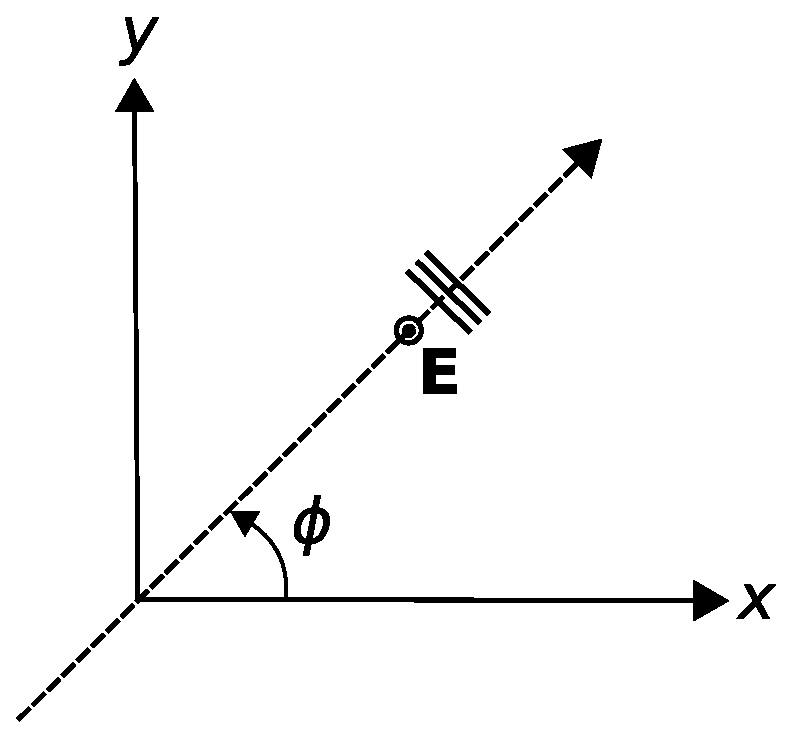
\includegraphics[width=2in]{modules/m0039_fEx1.eps}
% ***WikipediaCommonsURL
}}{An x-y plot with a dashed vector extending through the origin at an angle phi. On the vector at an arbitrary point is a circle, labeled E. Beside E on the vector are three straight parallel lines. }
\end{center} 
%\centerline{\scriptsize 
%\copyright~\hyperref[***_Credit]{author} 
%\href{https://creativecommons.org/licenses/by-sa/4.0/}{CC BY-SA 4.0} 
%} 
\caption{
\label{m0039_fEx1}
A radially-directed plane wave.
}
\end{figure}
\end{example}
%%%%%%%%%%%%%%%%%%%%%%%%%%%%%%%%%%%%%%%%%%%%%%%


{\bf Additional Reading:}
\begin{itemize}
\item ``\href{https://en.wikipedia.org/wiki/Electromagnetic_radiation}{Electromagnetic radiation}'' on Wikipedia.
\end{itemize}

\index{waves!plane|)}

      \vfill\break
    \section{Wave Polarization}
{\color{blue}\tiny[m0131]}      % This is text associated with the open textbook "Open Electromagnetics"
% See immediately below for author, date
% This work is licensed under the Creative Commons Attribution-ShareAlike 4.0 International License. (CC BY SA 4.0) 
% To view a copy of the license, visit http://creativecommons.org/licenses/by-sa/4.0/

%ORB TITLE Wave Polarization
%ORB AUTHOR 0        # S.W. Ellingson, Virginia Tech (ellingson@vt.edu)
%ORB DATE 20180807   # yyyymmdd
%ORB ABSTRACT Wave Polarization

\label{m0131_Wave_Polarization} % <-- Must match name of this file and module directory name.  Don't mess with this!
\index{polarization|}
\index{waves!polarization|(}

\emph{Polarization} refers to the orientation of the electric field vector.
For waves, the term ``polarization'' refers specifically to the orientation of this vector with increasing distance along the direction of propagation, or, equivalently, the orientation of this vector with increasing time at a fixed point in space.
The relevant concepts are readily demonstrated for uniform plane waves, as shown in this section.
A review of Section~\ref{m0039_Uniform_Plane_Waves_Characteristics} (``Uniform Plane Waves: Characteristics'') is recommended before reading further.

To begin, consider the following uniform plane wave, described in terms of the phasor representation of its electric field intensity:
%
\begin{equation}
\widetilde{\bf E}_x = \hat{\bf x}E_x e^{-j\beta z}
\end{equation}
%
Here $E_x$ is a complex-valued constant representing the magnitude and phase of the wave,
and $\beta$ is the positive real-valued propagation constant.  
Therefore, this wave is propagating in the $+\hat{\bf z}$ direction in lossless media.
This wave is said to exhibit \emph{linear} polarization 
\index{polarization!linear}
(and ``linearly polarized'')
 because the electric field always points in the same direction, namely $+\hat{\bf x}$.
Now consider the wave
%
\begin{equation}
\widetilde{\bf E}_y = \hat{\bf y}E_y e^{-j\beta z}
\end{equation}
%
Note that $\widetilde{\bf E}_y$ is identical to $\widetilde{\bf E}_x$ except that the electric field vector now points in the $+\hat{\bf y}$ direction and has magnitude and phase that is different by the factor $E_y/E_x$.
This wave too is said to exhibit linear polarization, because, again, the direction of the electric field is constant with both time and position.
In fact, \emph{all} linearly-polarized uniform plane waves propagating in the $+\hat{\bf z}$ direction in lossless media can be described as follows:
%
\begin{equation}
\widetilde{\bf E} = \hat{\bf \rho}E_{\rho} e^{-j\beta z}
\end{equation}
%
This is so because $\hat{\bf \rho}$ could be $\hat{\bf x}$, $\hat{\bf y}$, or any other direction that is perpendicular to $\hat{\bf z}$.
If one is determined to use Cartesian coordinates, the above expression may be rewritten using (Section~\ref{m0096_Cylindrical_Coordinates})
%
\begin{equation}
\hat{\bf \rho} = \hat{\bf x}\cos\phi + \hat{\bf y}\cos\phi
\end{equation}
%
yielding
%
\begin{equation}
\widetilde{\bf E} = \left( \hat{\bf x}\cos\phi + \hat{\bf y}\cos\phi \right) E_{\rho} e^{-j\beta z}
\label{m0131_eLinAI}
\end{equation}
%
When written in this form, 
$\phi=0$ corresponds to $\widetilde{\bf E}=\widetilde{\bf E}_x$,
$\phi=\pi/2$ corresponds to $\widetilde{\bf E}=\widetilde{\bf E}_y$,
and any other value of $\phi$ corresponds to some other constant orientation of the electric field vector;
see Figure~\ref{m0131_fLinearly_Polarized_Wave} for an example.
%
\begin{figure}
\begin{center}
\pdftooltip{{  % note double braces
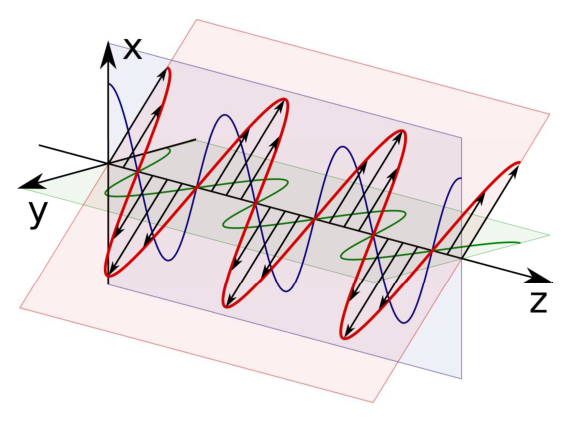
\includegraphics[width=\columnwidth]{modules/m0131_Linearly_Polarized_Wave.eps}
% https://commons.wikimedia.org/wiki/File:Linearly_Polarized_Wave.svg
}}{Similar to a previous figure. Cartesian coordinates with x (vertical), y (out-of-page), and z (horizontal) axes. A sinusoidal wave (blue) with a maximum at the x-intercept extends down the z-axis. Perpendicular to the first wave, the a second sinusoid (green) is in the y-z plane. At an angle phi equals pi over 4, sits a red plane, where the sinusoidal wave travels the length of the z axis at the angle phi. For both the red and green waves vectors point from the z-axis to the waveform.}
\end{center} 
\centerline{\scriptsize 
by~\hyperref[m0131_Linearly_Polarized_Wave_Credit]{RJB1} (Modified) 
} 
\caption{
\label{m0131_fLinearly_Polarized_Wave}
Linear polarization.  Here ${\bf E}_x$ is shown in blue, ${\bf E}_y$ is shown in green, and ${\bf E}$ is shown in red with black vector symbols.  In this example the phases of $E_x$ and $E_y$ are zero and $\phi=-\pi/4$.
}
\end{figure}


%ORB HIGHLIGHT
\begin{mdframed}[backgroundcolor=yellow!20,nobreak=true] 
A wave is said to exhibit linear polarization if the direction of the electric field vector does not vary with either time or position.
\end{mdframed}

Linear polarization arises when the source of the wave is linearly polarized.  
A common example is the wave radiated by a straight wire antenna, 
\index{antenna}
such as a dipole 
\index{antenna!dipole}
\index{dipole|see{antenna}}
or a monopole.
\index{antenna!monopole}
\index{monopole|see{antenna}}
Linear polarization may also be created by passing a plane wave through a \emph{polarizer}; 
\index{polarizer}
this is particularly common at optical frequencies (see ``Additional Reading'' at the end of this section).

A commonly-encountered alternative to linear polarization is \emph{circular polarization}.
\index{polarization!circular}
For an explanation, let us return to the linearly-polarized plane waves $\widetilde{\bf E}_x$ and $\widetilde{\bf E}_y$ defined earlier.
If both of these waves exist simultaneously, then the total electric field intensity is simply the sum:
%  
\begin{flalign}
\widetilde{\bf E} &= \widetilde{\bf E}_x +\widetilde{\bf E}_y  \nonumber \\
                  &= \left( \hat{\bf x}E_x + \hat{\bf y}E_y \right) e^{-j\beta z}  
\label{m0131_eCirc1}
\end{flalign}
%
If the phase of $E_x$ and $E_y$ is the same, then $E_x = E_{\rho}\cos\phi$, $E_y = E_{\rho}\sin\phi$, and the above expression is essentially the same as Equation~\ref{m0131_eLinAI}.
In this case, $\widetilde{\bf E}$ is linearly polarized.
But what if the phases of $E_x$ and $E_y$ are different?
In particular, let's consider the following case. Let $E_x = E_0$, some complex-valued constant, and let $E_y = +jE_0$, which is $E_0$ phase-shifted by $+\pi/2$ radians. 
With no further math, it is apparent that $\widetilde{\bf E}_x$ and $\widetilde{\bf E}_y$ are different only in that one is phase-shifted by $\pi/2$ radians relative to the other.
For the physical (real-valued) fields, this means that ${\bf E}_x$ has maximum magnitude when ${\bf E}_y$ is zero and vice versa.
As a result, the direction of ${\bf E}={\bf E}_x+{\bf E}_y$ will rotate in the $x-y$ plane, as shown in Figure~\ref{m0131_fCircular_Polarized_Wave}
%
\begin{figure}
\begin{center}
\pdftooltip{{  % note double braces
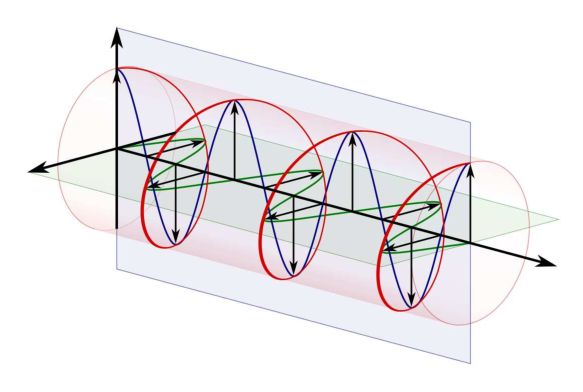
\includegraphics[width=\columnwidth]{modules/m0131_Circular.Polarization.Circularly.Polarized.Light_With.Components_Left.Handed.eps}
% https://en.wikipedia.org/wiki/File:Circular.Polarization.Circularly.Polarized.Light_With.Components_Left.Handed.svg
}}{Similar to a previous figure, except the xyz coordinates show only the blue and green planes and waves. Black vectors extend from the z-axis to the top of the waves in the blue and green planes. A red path connects the peaks of each wave in a circular manner as it travels the z-axis. The final image looks like a coil of wire with a vertical and horizontal sinusoidal wave inside it.}
\end{center} 
\centerline{\scriptsize 
by~\hyperref[m0131_Circular.Polarization.Circularly.Polarized.Light_With.Components_Left.Handed_Credit]{Dave3457} 
} 
\caption{
\label{m0131_fCircular_Polarized_Wave}
A circularly-polarized wave (in red, with black vector symbols) resulting from the addition of orthogonal linearly-polarized waves (shown in green and blue) that are phase-shifted by $\pi/2$ radians.
}
\end{figure}

The rotation of the electric field vector can also be identified mathematically.  When $E_x = E_0$ and $E_y = +jE_0$, Equation~\ref{m0131_eCirc1} can be written:
%  
\begin{equation}
\widetilde{\bf E} = \left( \hat{\bf x} + j\hat{\bf y} \right) E_0 e^{-j\beta z}  
\end{equation}
%
Now reverting from phasor 
\index{phasor}
notation to the physical field:
%  
\begin{flalign}
{\bf E} &= \mbox{Re}\left\{ \widetilde{\bf E} e^{j\omega t} \right\} \nonumber \\
        &= \mbox{Re}\left\{ \left( \hat{\bf x} + j\hat{\bf y} \right) E_0 e^{-j\beta z} e^{j\omega t} \right\} \nonumber \\
        &= \hat{\bf x} \left|E_0\right| \cos\left(\omega t - \beta z \right) + \hat{\bf y} \left|E_0\right| \cos\left(\omega t - \beta z +\frac{\pi}{2} \right) 
\end{flalign}
%
As anticipated, we see that both ${\bf E}_x$ and ${\bf E}_y$ vary sinusoidally, but are $\pi/2$ radians out of phase resulting in rotation in the plane perpendicular to the direction of propagation.

In the example above, the electric field vector rotates either clockwise or counter-clockwise relative to the direction of propagation.  The direction of this rotation can be identified by pointing the thumb of the left hand in the direction of propagation; in this case, the fingers of the left hand curl in the direction of rotation.  For this reason, this particular form of circular polarization is known as \emph{left circular} (or ''left-hand'' circular) polarization (LCP).  
If we instead had chosen $E_y = -jE_0 = -jE_x$, then the direction of ${\bf E}$ rotates in the opposite direction, giving rise to \emph{right circular} (or ``right-hand'' circular) polarization (RCP).
These two conditions are illustrated in Figure~\ref{m0131_fLCP-RCP}.
%
\begin{figure}
\begin{center}
\pdftooltip{{  % note double brace
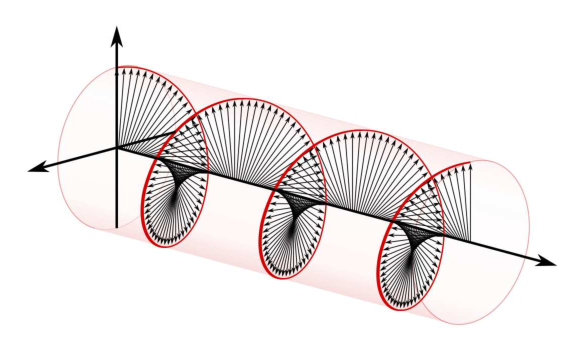
\includegraphics[width=\columnwidth]{modules/m0131_Circular.Polarization.Circularly.Polarized.Light_Without.Components_Left.Handed.eps}
% https://en.wikipedia.org/wiki/File:Circular.Polarization.Circularly.Polarized.Light_Without.Components_Left.Handed.svg
}}{Similar to a previous figure, a red coil encompasses the z-axis. Arrow vectors start at the z-axis and meet the coil. The upper coil, left circular polarization, starting at the origin appears to go into and then out of the page. In contrast the lower coil, right circular polarization, starting at the origin appears to come out of the page and then go into the page.}
\end{center} 
\begin{center}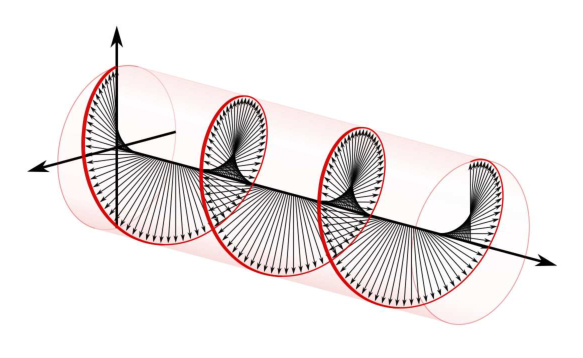
\includegraphics[width=\columnwidth]{modules/m0131_Circular.Polarization.Circularly.Polarized.Light_Without.Components_Right.Handed.eps}\end{center} 
% https://en.wikipedia.org/wiki/File:Circular.Polarization.Circularly.Polarized.Light_Without.Components_Left.Handed.svg
\centerline{\scriptsize 
by~\hyperref[m0131_Circular.Polarization.Circularly.Polarized.Light_Without.Components_Credit]{Dave3457} 
} 
\caption{
\label{m0131_fLCP-RCP}
Left-circular polarization (LCP; top) and right-circular polarization (RCP; bottom).
}
\end{figure}

%ORB HIGHLIGHT
\begin{mdframed}[backgroundcolor=yellow!20,nobreak=true] 
A wave is said to exhibit circular polarization if the electric field vector rotates with constant magnitude.  Left- and right-circular polarizations may be identified by the direction of rotation with respect to the direction of propagation. 
\end{mdframed}

In engineering applications, circular polarization is useful when the relative orientations of transmit and receive equipment is variable and/or when the medium is able rotate the electric field vector.  For example, radio communications involving satellites in non-geosynchronous orbits typically employ circular polarization.
In particular, satellites of the U.S. Global Positioning System (GPS) 
\index{Global Positioning System (GPS)}
transmit circular polarization because of the variable geometry of the space-to-earth radio link and the tendency of the Earth's ionosphere to rotate the electric field vector through a mechanism known \emph{Faraday rotation} 
\index{Faraday rotation}
(sometimes called the ``Faraday effect'').
If GPS were instead to transmit using a linear polarization, then a receiver would need to continuously adjust the orientation of its antenna in order to optimally receive the signal.   
Circularly-polarized radio waves can be generated (or received) using pairs of perpendicularly-oriented dipoles that are fed the same signal but with a $90^{\circ}$ phase shift, or alternatively by using an antenna that is intrinsically circularly-polarized, such as a helical antenna 
\index{antenna!helical}
(see ``Additional Reading'' at the end of this section). 

Linear and circular polarization are certainly not the only possibilities.
\emph{Elliptical polarization} 
\index{polarization!elliptical}
results when $E_x$ and $E_y$ do not have equal magnitude.
Elliptical polarization is typically not an intended condition, but rather is most commonly observed as a degradation in a system that is nominally linearly- or circularly-polarized.  For example, most antennas that are said to be ``circularly polarized'' instead produce circular polarization only in one direction and various degrees of elliptical polarization in all other directions.   

{\bf Additional Reading:}
\begin{itemize}
\item ``\href{https://en.wikipedia.org/wiki/Polarization_(waves)}{Polarization (waves)}'' on Wikipedia.
\item ``\href{https://en.wikipedia.org/wiki/Dipole_antenna}{Dipole antenna}'' on Wikipedia.
\item ``\href{https://en.wikipedia.org/wiki/Polarizer}{Polarizer}'' on Wikipedia.
\item ``\href{https://en.wikipedia.org/wiki/Faraday_effect}{Faraday effect}'' on Wikipedia.
\item ``\href{https://en.wikipedia.org/wiki/Helical_antenna}{Helical antenna}'' on Wikipedia.
\end{itemize}

\index{waves!polarization|)}

      \vfill\break
    \section{Wave Power in a Lossless Medium}
{\color{blue}\tiny[m0041]}      % This is text associated with the open textbook "Open Electromagnetics"
% See immediately below for author, date
% This work is licensed under the Creative Commons Attribution-ShareAlike 4.0 International License. (CC BY SA 4.0) 
% To view a copy of the license, visit http://creativecommons.org/licenses/by-sa/4.0/

%ORB TITLE Wave Power in a Lossless Medium
%ORB AUTHOR 0        # S.W. Ellingson, Virginia Tech (ellingson@vt.edu)
%ORB DATE 20180807   # yyyymmdd
%ORB ABSTRACT Plane Wave Power Density in a Lossless Medium 

\label{m00041_Plane_Wave_Power_Density_in_a_Lossless_Medium} % <-- Must match name of this file and module directory name.  Don't mess with this!
\index{waves!power density|(}
\index{power density|see{waves}}

In many applications involving electromagnetic waves, one is less concerned with the instantaneous values of the electric and magnetic fields than the \emph{power} associated with the wave. 
In this section, we address the issue of how much power is conveyed by an electromagnetic wave in a lossless medium.
The relevant concepts are readily demonstrated in the context of uniform plane waves, 
\index{waves!plane}
as shown in this section.
A review of Section~\ref{m0039_Uniform_Plane_Waves_Characteristics} (``Uniform Plane Waves: Characteristics'') is recommended before reading further.

Consider the following uniform plane wave, described in terms of the phasor representation of its electric field intensity:
%
\begin{equation}
\widetilde{\bf E} = \hat{\bf x}E_0 e^{-j\beta z}
\label{m0041_eE}
\end{equation}
%
Here $E_0$ is a complex-valued constant associated with the source of the wave, and $\beta$ is the positive real-valued propagation constant.  
Therefore, the wave is propagating in the $+\hat{\bf z}$ direction in lossless media.

The first thing that should be apparent is that the amount of power conveyed by this wave is infinite.
The reason is as follows. If the power passing through any finite area is greater than zero, then the total power must be infinite because, for a uniform plane wave, the electric and magnetic field intensities are constant over a plane of infinite area.
In practice, we never encounter this situation because all practical plane waves are only ``locally planar'' (see Section~\ref{m0142_Types_of_Waves} for a refresher on this idea).
Nevertheless, we seek some way to express the power associated with such waves.

The solution is not to seek total power, but rather power per unit area.
This quantity is known as the \emph{spatial power density}, or simply ``\emph{power density},'' and has units of W/m$^2$.\footnote{Be careful: The quantities \emph{power spectral density} (W/Hz) and \emph{power flux density} (W/(m$^2\cdot$Hz)) are also sometimes referred to as ``power density.''  In this section, we will limit the scope to \emph{spatial} power density (W/m$^2$).} 
Then, if we are interested in total power passing through some finite area, then we may simply integrate the power density over this area.
Let's skip to the answer, and then consider where this answer comes from.
It turns out that the \emph{instantaneous} power density of a uniform plane wave is the magnitude of the \emph{Poynting vector}
\index{Poynting vector}
%
\begin{equation}
{\bf S} \triangleq {\bf E} \times {\bf H}
\label{m0041_eS}
\end{equation}
%
Note that this equation is dimensionally correct; i.e. the units of ${\bf E}$ (V/m) times the units of ${\bf H}$ (A/m) yield the units of spatial power density (V$\cdot$A/m$^2$, which is W/m$^2$).
Also, the direction of ${\bf E} \times {\bf H}$ is in the direction of propagation (reminder: Section~\ref{m0039_Uniform_Plane_Waves_Characteristics}), which is the direction in which the power is expected to flow.
Thus, we have some compelling evidence that $\left|{\bf S}\right|$ is the power density we seek.
However, this is not proof -- for that, we require the \emph{Poynting Theorem}, 
\index{Poynting theorem}
which is a bit outside the scope of the present section, but is addressed in the ``Additional Reading'' at the end of this section.

A bit later we're going to need to know ${\bf S}$ for a uniform plane wave, so let's work that out now.
From the plane wave relationships (Section~\ref{m0039_Uniform_Plane_Waves_Characteristics}) we find that the magnetic field intensity associated with the electric field in Equation~\ref{m0041_eE} is
%
\begin{equation}
\widetilde{\bf H} = \hat{\bf y}\frac{E_0}{\eta} e^{-j\beta z}
\label{m0041_eH}
\end{equation}
%
where $\eta=\sqrt{\mu/\epsilon}$ is the real-valued impedance of the medium.
Let $\psi$ be the phase of $E_0$; i.e., $E_0 = |E_0|e^{j\psi}$.
Then
%
\begin{flalign}
{\bf E} &=  \mbox{Re}\left\{ \widetilde{\bf E} e^{j\omega t} \right\}  \nonumber \\
        &= \hat{\bf x}\left|E_0\right| \cos\left( \omega t - \beta z + \psi \right)
\end{flalign}
%
and
%
\begin{flalign}
{\bf H} &=  \mbox{Re}\left\{ \widetilde{\bf H} e^{j\omega t} \right\}  \nonumber \\
        &= \hat{\bf y}\frac{\left|E_0\right|}{\eta} \cos\left( \omega t - \beta z + \psi \right)
\end{flalign}
%
Now applying Equation~\ref{m0041_eS},
%
\begin{equation}
{\bf S} =\hat{\bf z} \frac{|E_0|^2}{\eta} \cos^2\left( \omega t - \beta z + \psi \right)
\end{equation} 

As noted earlier, $\left|{\bf S}\right|$ is only the instantaneous power density, which is still not quite what we are looking for.
What we are actually looking for is the \emph{time-average} power density $S_{ave}$ -- that is, the average value of $\left|{\bf S}\right|$ over one period $T$ of the wave.
This may be calculated as follows:
%
\begin{flalign}
S_{ave} &= \frac{1}{T} \int_{t=t_0}^{t_0+T} |{\bf S}| dt \nonumber \\
        &= \frac{|E_0|^2}{\eta} \frac{1}{T} \int_{t=t_0}^{t_0+T}  \cos^2\left( \omega t - ks + \psi \right)  dt
\end{flalign}
%
Since $\omega =2\pi f = 2\pi/T$, the definite integral equals $T/2$.  We obtain
%
\begin{equation}
\boxed{ S_{ave} = \frac{|E_0|^2}{2\eta} }
\label{m0041_eWEPWD}
\end{equation}
%
It is useful to check units again at this point.  Note (V/m)$^2$ divided by $\Omega$ is W/m$^2$, as expected.  
%
%ORB HIGHLIGHT
\begin{mdframed}[backgroundcolor=yellow!20,nobreak=true] 
Equation~\ref{m0041_eWEPWD} is the time-average power density (units of W/m$^2$) associated with a sinusoidally-varying uniform plane wave in lossless media.
\end{mdframed}

Note that Equation~\ref{m0041_eWEPWD} is analogous to a well-known result from electric circuit theory. Recall the time-average power $P_{ave}$ (units of W) associated with a voltage phasor $\widetilde{V}$ across a resistance $R$ is 
%
\begin{equation}
P_{ave} = \frac{|\widetilde{V}|^2}{2R}
\label{m0041_ePWLM-EA}
\end{equation}
%
which closely resembles Equation~\ref{m0041_eWEPWD}.
The result is also analogous to the result for a voltage wave on a transmission line (Section~\ref{m0090_Power_Flow_on_Transmission_Lines}), for which: 
%
\begin{equation}
P_{ave} = \frac{|V_0^+|^2}{2Z_0}
\end{equation}
%
where $V_0^+$ is a complex-valued constant representing the magnitude and phase of the voltage wave, and $Z_0$ is the characteristic impedance 
\index{characteristic impedance}
of the transmission line.
\index{waves!transmission line analogy}

Here is a good point at which to identify a common pitfall. $|E_0|$ and $|\widetilde{V}|$ are the {\it peak magnitudes} of the associated real-valued physical quantities.  However, these quantities are also routinely given as {\it root mean square} (``rms'') quantities.  Peak magnitudes are greater by a factor of $\sqrt{2}$, so Equation~\ref{m0041_eWEPWD} expressed in terms of the rms quantity lacks the factor of $1/2$.  

%%%%%%%%%%%%%%%%%%%%%%%%%%%%%%%%%%%%%%%%%%%%%%%
%ORB EXAMPLE
~\\ \begin{example} 
\begin{mdframed}[backgroundcolor=brown!20,linecolor=brown!20]\raggedright
Power density of a typical radio wave.
\\~\\
A radio wave transmitted from a distant location may be perceived locally as a uniform plane wave if there is no nearby structure to scatter the wave; a good example of this is the wave arriving at the user of a cellular telephone in a rural area with no significant terrain scattering.  The range of possible signal strengths varies widely, but a typical value of the electric field intensity arriving at the user's location is 10~$\mu$V/m rms.  What is the corresponding power density?

{\bf Solution}:  From the problem statement, $|E_0|=10~\mu$V/m rms.
We assume propagation occurs in air, which is indistinguishable from free space at cellular frequencies.  
If we use Equation~\ref{m0041_eWEPWD}, then we must first convert $|E_0|$ from rms to peak magnitude, which is done by multiplying by $\sqrt{2}$.  Thus:
%
\begin{flalign}
S_{ave} &= \frac{|E_0|^2}{2\eta} \cong \frac{\left(\sqrt{2} \cdot 10 \times 10^{-6}~\mbox{V/m}\right)^2}{2 \cdot 377~\Omega} \nonumber \\
        &\cong 2.65 \times 10^{-13}~\mbox{W/m$^2$} \nonumber
\end{flalign}
%
Alternatively, we can just use a version of Equation~\ref{m0041_eWEPWD}, which is appropriate for rms units:
%
\begin{flalign}
S_{ave} &= \frac{|E_{0,rms}|^2}{\eta} \cong \frac{\left(10 \times 10^{-6}~\mbox{V/m}\right)^2}{ 377~\Omega} \nonumber \\
        &\cong 2.65 \times 10^{-13}~\mbox{W/m$^2$} \nonumber
\end{flalign}
%
Either way, we obtain the correct answer, 0.265~pW/m$^2$ (that's {\it picowatts} per square meter).

\end{mdframed}
% note figures will need to go between "\end{mdframed}" and "\end{example}"
\end{example}
%%%%%%%%%%%%%%%%%%%%%%%%%%%%%%%%%%%%%%%%%%%%%%%


Considering the prevalence of phasor representation, it is useful to have an alternative form of the Poynting vector which yields time-average power by operating directly on field quantities in phasor form.  This is ${\bf S}_{ave}$, defined as:
%
\begin{equation}
{\bf S}_{ave} \triangleq \frac{1}{2} \mbox{Re} \left\{ \widetilde{\bf E} \times \widetilde{\bf H}^* \right\}
\end{equation}
%
(Note that the magnetic field intensity phasor is conjugated.)  
The above expression gives the expected result for a uniform plane wave.
Using Equations~\ref{m0041_eE} and \ref{m0041_eH}, we find
%
\begin{equation}
{\bf S}_{ave} = \frac{1}{2} \mbox{Re} \left\{
  \left( \hat{\bf x}E_0 e^{-j\beta z} \right)
\times
  \left( \hat{\bf y}\frac{E_0}{\eta} e^{-j\beta z} \right)^* \right\}
\end{equation}
%
which yields
%
\begin{equation}
{\bf S}_{ave} = \hat{\bf z}\frac{|E_0|^2}{2\eta} 
\end{equation}
%
as expected.  
%The details of the derivation are not difficult and are left as an exercise for the reader.

%Although we have developed the Poynting vector concept from a scenario involving a single uniform plane wave, it should be noted that the concept applies to {\it any} wave or combination of waves.  This is verifiably so since in the scenario we considered we did not need to specify the volume of $\mathcal{V}$ nor the area of $A$ or $B$.  Thus, these dimensions could be made arbitrarily small, such that any wave appears planar and uniform to arbitrarily good accuracy.  

{\bf Additional Reading:}
\begin{itemize}
\item ``\href{https://en.wikipedia.org/wiki/Poynting_vector}{Poynting vector}'' on Wikipedia.
\item ``\href{https://en.wikipedia.org/wiki/Poynting's_theorem}{Poynting's Theorem}'' on Wikipedia.
\end{itemize}    

\index{waves!power density|)}

%%%      \vfill\break
{\color{blue}\tiny[m0035]}    % This is text associated with the open textbook "Open Electromagnetics"
% See immediately below for author, date
% This work is licensed under the Creative Commons Attribution-ShareAlike 4.0 International License. (CC BY SA 4.0) 
% To view a copy of the license, visit http://creativecommons.org/licenses/by-sa/4.0/

%ORB TITLE Plane Wave Propagation in Lossless Media
%ORB AUTHOR 0        # S.W. Ellingson, Virginia Tech (ellingson@vt.edu)
%ORB DATE 20180701   # yyyymmdd
%ORB ABSTRACT End matter for chapter entitled "Plane Wave Propagation in Lossless Media"

\label{m0035_Ch_End_Matter_Plane_Wave_Prop_Lossless} % <-- Must match name of this file and module directory name.  Don't mess with this!

\onecolumn
\section*{Image Credits}

\begin{itemize}

\item[Fig.] \label{m0142_fSphericalPhasefront_Credit}
  \ref{m0142_fSphericalPhasefront}:
  \copyright~Y.\ Qin, 
  \url{https://commons.wikimedia.org/wiki/File:M0142_fSphericalPhasefront.svg},\\ 
  CC BY 4.0 (\url{https://creativecommons.org/licenses/by/4.0/}).

\item[Fig.] \label{m0142_fCylindricalPhasefront_Credit}
  \ref{m0142_fCylindricalPhasefront}
  \copyright~Y.\ Qin, 
  \url{https://commons.wikimedia.org/wiki/File:M0142_fCylindricalPhasefront.svg},\\ 
  CC BY 4.0 (\url{https://creativecommons.org/licenses/by/4.0/}).

\item[Fig.] \label{m0142_fPlanarPhasefront_Credit}
  \ref{m0142_fPlanarPhasefront}
  \copyright~Y.\ Qin, 
  \url{https://commons.wikimedia.org/wiki/File:M0142_fPlanarPhasefront.svg},\\ 
  CC BY 4.0 (\url{https://creativecommons.org/licenses/by/4.0/}).

\item[Fig.] \label{m0142_fPlaneWavesReflector_Credit}
  \ref{m0142_fPlaneWavesReflector}
  \copyright~Y.\ Qin, 
  \url{https://commons.wikimedia.org/wiki/File:M0142_fPlaneWavesReflector.svg},\\ 
  CC BY 4.0 (\url{https://creativecommons.org/licenses/by/4.0/}).

\item[Fig.] \label{m0142_fLocallyPlanar_Credit}
  \ref{m0142_fLocallyPlanar}
  \copyright~Y.\ Qin, 
  \url{https://commons.wikimedia.org/wiki/File:M0142_fLocallyPlanar.svg},\\ 
  CC BY 4.0 (\url{https://creativecommons.org/licenses/by/4.0/}).

\item[Fig.] \label{m0039_Onde_electromagnetique_Credit}
  \ref{m0039_fPWR}:
  \copyright~E.\ Boutet, 
  {\footnotesize \url{https://en.wikipedia.org/wiki/File:Onde_electromagnetique.svg}},\\ 
  CC BY~SA 3.0 (\url{https://creativecommons.org/licenses/by-sa/3.0/}).
  Heavily modified by author.

\item[Fig.] \label{m0131_Linearly_Polarized_Wave_Credit}
  \ref{m0131_fLinearly_Polarized_Wave}:
  RJB1, 
  \url{https://commons.wikimedia.org/wiki/File:Linearly_Polarized_Wave.svg},\\ 
  public domain.
  Modified by author.

\item[Fig.] \label{m0131_Circular.Polarization.Circularly.Polarized.Light_With.Components_Left.Handed_Credit}
  \ref{m0131_fCircular_Polarized_Wave}:
  Dave3457, 
  %\url{https://en.wikipedia.org/wiki/File:Circular.Polarization.Circularly.Polarized.Light_With.Components_Left.Handed.svg},\\ 
  {https://en.wikipedia.org/wiki/File:Circular.Polarization.Circularly.Polarized.Light\\\_With.Components\_Left.Handed.svg},\\ 
  public domain.

\item[Fig.] \label{m0131_Circular.Polarization.Circularly.Polarized.Light_Without.Components_Credit}
  \ref{m0131_fLCP-RCP}:
  Dave3457, 
  %\url{https://en.wikipedia.org/wiki/File:Circular.Polarization.Circularly.Polarized.Light_Without.Components_Left.Handed.svg} 
  {https://en.wikipedia.org/wiki/File:Circular.Polarization.Circularly.Polarized.Light\\\_Without.Components\_Left.Handed.svg}\\ 
and
  %\url{https://en.wikipedia.org/wiki/File:Circular.Polarization.Circularly.Polarized.Light_Without.Components_Right.Handed.svg},\\ 
  {https://en.wikipedia.org/wiki/File:Circular.Polarization.Circularly.Polarized.Light\\
\_Without.Components\_Right.Handed.svg},\\ 
  public domain.

\end{itemize}

\twocolumn

\appendix
  \chapter{Constitutive Parameters of Some Common Materials}
  \thispagestyle{fancy} % override footer in first page of chapter
  \fancyhf{}            % reset header and footer
  \fancyfoot[C]{\footnotesize \emph{Electromagnetics Vol~1}. ~\copyright~2018 S.W.\ Ellingson ~CC~BY~SA~4.0. ~\url{https://doi.org/10.21061/electromagnetics-vol-1}}
    \section{Permittivity of Some Common Materials}
{\color{blue}\tiny[m0135]}      % This is text associated with the open textbook "Open Electromagnetics"
% See immediately below for author, date
% This work is licensed under the Creative Commons Attribution-ShareAlike 4.0 International License. (CC BY SA 4.0) 
% To view a copy of the license, visit http://creativecommons.org/licenses/by-sa/4.0/

%ORB TITLE Permittivity of Some Common Materials
%ORB AUTHOR 0        # S.W. Ellingson, Virginia Tech (ellingson@vt.edu)
%ORB DATE 20180807   # yyyymmdd
%ORB ABSTRACT Permittivity of Some Commonly-Encountered Materials Materials

\label{m0135_Table_of_Permittivities} % <-- Must match name of this file and module directory name.  Don't mess with this!
\index{permittivity!of common materials|(}

The values below are relative permittivity $\epsilon_r \triangleq \epsilon/\epsilon_0$ for a few materials that are commonly encountered in electrical engineering applications, and for which permittivity emerges as a consideration.
Note that ``relative permittivity'' 
\index{permittivity!relative}
is sometimes referred to as \emph{dielectric constant}.
\index{dielectric constant}

Here we consider only the physical (real-valued) permittivity, which is the real part of the complex permittivity (typically indicated as $\epsilon'$ or $\epsilon_r'$) for materials exhibiting significant loss.

Permittivity varies significantly as a function of frequency.
The values below are representative of frequencies from a few kHz to about 1~GHz.
The values given are also representative of optical frequencies for materials such as silica that are used in optical applications.
Permittivity also varies as a function of temperature.
In applications where precision better than about 10\% is required, primary references accounting for frequency and temperature should be consulted.
The values presented here are gathered from a variety of references, including those indicated in ``Additional References.''
  
{\bf Free Space} (vacuum): $\epsilon_r \triangleq 1$

\vfill\break
{\bf Solid Dielectrics}:
\index{dielectric (material)!examples}
%
\begin{tabular}{lll}
Material                   & $\epsilon_r$ & Common uses \\
\hline
Styrofoam$^1$              & 1.1 & \\ \index{styrofoam} % https://en.wikipedia.org/wiki/Styrofoam 
Teflon$^2$                 & 2.1 & \\ \index{teflon} % HPC, https://en.wikipedia.org/wiki/Polytetrafluoroethylene
Polyethylene               & 2.3 & coaxial cable \index{polyethylene} \\ % HPC
Polypropylene              & 2.3 & \\ \index{polypropylene} % HPC
Silica                     & 2.4 & optical fiber$^3$ \index{silica} \\ %https://en.wikipedia.org/wiki/Optical_fiber
Polystyrene                & 2.6 & \\ \index{polystyrene} % HPC, https://en.wikipedia.org/wiki/Polystyrene
Polycarbonate              & 2.8 & \\ \index{polycarbonate} % HPC, https://en.wikipedia.org/wiki/Polycarbonate
Rogers RO3003              & 3.0 & PCB substrate \\ \index{printed circuit board (PCB)!material}
FR4 (glass epoxy laminate) & 4.5 & PCB substrate \index{FR4} \\ % https://en.wikipedia.org/wiki/FR-4
\end{tabular}
%
~\\
$^1$ Properly known as \emph{extruded polystyrene foam} (XPS).\\
$^2$ Properly known as \emph{polytetrafluoroethylene} (PTFE).\\ \index{polytetrafluoroethylene}
$^3$ Typically doped with small amounts of other materials to slightly raise or lower the index of refraction 
\index{index of refraction}
($=\sqrt{\epsilon_r}$).

Non-conducting spacing materials used in discrete capacitors exhibit $\epsilon_r$ ranging from about 5 to 50.

{\bf Semiconductors} 
\index{semiconductor (material)}
commonly appearing in electronics -- including carbon, silicon, 
\index{silicon}
geranium, 
\index{geranium}
indium phosphide, 
\index{indium phosphide}
and so on -- typically exhibit $\epsilon_r$ in the range 5--15.  
% https://www.microwaves101.com/encyclopedias/indium-phosphide

{\bf Glass} 
\index{glass}
exhibits $\epsilon_r$ in the range 4--10, depending on composition.

{\bf Gasses}, including air, typically exhibit $\epsilon_r\cong 1$ to within a tiny fraction of a percent. 

{\bf Liquid water} 
\index{water}
typically exhibits $\epsilon_r$ in the range 72--81. Distilled water exhibits $\epsilon_r \approx 81$ at room temperature, whereas sea water tends to be at the lower end of the range.    

{\bf Other liquids} typically exhibit $\epsilon_r$ in the range 10--90, with considerable variation as a function of temperature and frequency.  Animal flesh and blood consists primarily of liquid matter and so also exhibits permittivity in this range.

{\bf Soil} 
\index{soil}
typically exhibits $\epsilon_r$ in the range 2.5--3.5 when dry and higher when wet.  The permittivity of soil varies considerably depending on composition.

%--------------------------------

{\bf Additional Reading:}
\begin{itemize}
\item \href{http://hbcponline.com}{\emph{CRC Handbook of Chemistry and Physics}}.
\item ``\href{https://en.wikipedia.org/wiki/Relative_permittivity}{Relative permittivity}'' on Wikipedia.
\item ``\href{http://www.microwaves101.com/encyclopedias/miscellaneous-dielectric-constants}{Miscellaneous Dielectric Constants}'' on \href{http://www.microwaves101.com}{microwaves101.com}.
\end{itemize}

\index{permittivity!of common materials|)}



      \vfill\break
    \section{Permeability of Some Common Materials}
{\color{blue}\tiny[m0136]}      % This is text associated with the open textbook "Open Electromagnetics"
% See immediately below for author, date
% This work is licensed under the Creative Commons Attribution-ShareAlike 4.0 International License. (CC BY SA 4.0) 
% To view a copy of the license, visit http://creativecommons.org/licenses/by-sa/4.0/

%ORB TITLE Permeability of Some Common Materials
%ORB AUTHOR 0        # S.W. Ellingson, Virginia Tech (ellingson@vt.edu)
%ORB DATE 20180807   # yyyymmdd
%ORB ABSTRACT Permeability of Some Commonly-Encountered Materials Materials

\label{m0136_Table_of_Permeabilities} % <-- Must match name of this file and module directory name.  Don't mess with this!
\index{permeability!of common materials|(}

The values below are relative permeability 
\index{permeability!relative}
$\mu_r \triangleq \mu/\mu_0$ for a few materials that are commonly encountered in electrical engineering applications, and for which $\mu_r$ is significantly different from $1$. These materials are predominantly ferromagnetic metals and (in the case of ferrites) materials containing significant ferromagnetic metal content.
Nearly all other materials exhibit $\mu_r$ that is not significantly different from that of free space.

The values presented here are gathered from a variety of references, including those indicated in ``Additional References'' at the end of this section.
Be aware that permeability may vary significantly with frequency; values given here are applicable to the frequency ranges for applications in which these materials are typically used.
Also be aware that materials exhibiting high permeability are also typically non-linear; that is, permeability depends on the magnitude of the magnetic field.
Again, values reported here are those applicable to applications in which these materials are typically used.  

{\bf Free Space} (vacuum): $\mu_r\triangleq 1$.

{\bf Iron} 
\index{iron}
(also referred to by the chemical notation ``Fe'') appears as a principal ingredient in many materials and alloys employed in electrical structures and devices.
Iron exhibits $\mu_r$ that is very high, but which decreases with decreasing purity.  
99.95\% pure iron exhibits $\mu_r\sim 200,000$.
This decreases to $\sim 5000$ at 99.8\% purity and is typically below 100 for purity less than 99\%. 

{\bf Steel} 
\index{steel}
is an iron alloy that comes in many forms, with a correspondingly broad range of permeabilites. 
\emph{Electrical steel}, commonly used in electrical machinery and transformers when high permeability is desired, exhibits $\mu_r\sim 4000$. % https://en.wikipedia.org/wiki/Electrical_steel
\emph{Stainless steel}, encompassing a broad range of alloys used in mechanical applications, exhibits $\mu_r$ in the range 750--1800. % https://en.wikipedia.org/wiki/Stainless_steel
\emph{Carbon steel}, including a broad class of alloys commonly used in structural applications,  exhibits $\mu_r$ on the order of 100. %https://en.wikipedia.org/wiki/Carbon_steel

{\bf Ferrites} 
\index{ferrite}
include a broad range of ceramic materials that are combined with iron and various combinations of other metals and are used as magnets and magnetic devices in various  electrical systems. Common ferrites exhibit $\mu_r$ in the range 16--640.

%--------------------------------

{\bf Additional Reading:}
\begin{itemize}
\item Section~\ref{m0058_Magnetic_Materials} (``Magnetic Materials'')
\item \href{http://hbcponline.com}{\emph{CRC Handbook of Chemistry and Physics}}.
\item ``\href{https://www.microwaves101.com/encyclopedias/magnetic-materials}{Magnetic Materials}'' on \href{http://www.microwaves101.com}{microwaves101.com}.
\item ``\href{https://en.wikipedia.org/wiki/Permeability_(electromagnetism)}{Permeability (electromagnetism)}'' on Wikipedia.
\item ``\href{https://en.wikipedia.org/wiki/Iron}{Iron}'' on Wikipedia.
\item ``\href{https://en.wikipedia.org/wiki/Electrical_steel}{Electrical steel}'' on Wikipedia.
\item ``\href{https://en.wikipedia.org/wiki/Ferrite_(magnet)}{Ferrite (magnet)}'' on Wikipedia.
\end{itemize}

\index{permeability!of common materials|)}

      \vfill\break
    \section{Conductivity of Some Common Materials}
{\color{blue}\tiny[m0137]}      % This is text associated with the open textbook "Open Electromagnetics"
% See immediately below for author, date
% This work is licensed under the Creative Commons Attribution-ShareAlike 4.0 International License. (CC BY SA 4.0) 
% To view a copy of the license, visit http://creativecommons.org/licenses/by-sa/4.0/

%ORB TITLE Conductivity of Some Common Materials
%ORB AUTHOR 0        # S.W. Ellingson, Virginia Tech (ellingson@vt.edu)
%ORB DATE 20180807   # yyyymmdd
%ORB ABSTRACT Conductivity of Some Commonly-Encountered Materials Materials

\label{m0137_Table_of_Conductivities} % <-- Must match name of this file and module directory name.  Don't mess with this!
\index{conductivity!of common materials|(}

The values below are conductivity $\sigma$ for a few materials that are commonly encountered in electrical engineering applications, and for which conductivity emerges as a consideration.

Note that materials in some applications are described instead in terms of \emph{resistivity}, 
\index{resistivity}
which is simply the reciprocal of conductivity.

Conductivity may vary significantly as a function of frequency.
The values below are representative of frequencies from a few kHz to a few GHz.
Conductivity also varies as a function of temperature.
In applications where precise values are required, primary references accounting for frequency and temperature should be consulted.
The values presented here are gathered from a variety of references, including those indicated in ``Additional References'' at the end of this section.
  
{\bf Free Space} (vacuum): $\sigma\triangleq 0$.

{\bf Commonly encountered elements}:\\
%
\begin{tabular}{ll}
Material                   & $\sigma$ (S/m) \\
\hline
Copper		& $5.8\times 10^7$   \\ \index{copper} % HCP
Gold		& $4.4\times 10^7$   \\ \index{gold} % HCP
Aluminum	& $3.7\times 10^7$   \\ \index{aluminum} % HCP
Iron		& $1.0\times 10^7$   \\ \index{iron} % Wikipedia page "Iron"
Platinum	& $0.9\times 10^7$   \\ \index{platinum} % HCP
Carbon		& $1.3\times 10^5$   \\ \index{carbon} % Wikipedia page "Carbon"
Silicon		& $4.4\times 10^{-4}$\\ \index{silicon} % Wikipedia page "Silicon"
\end{tabular}

{\bf Water} 
\index{water}
exhibits $\sigma$ ranging from 
about $6~\mu$S/m for highly distilled water (thus, a very poor conductor) to % HCP and Wikipedia.
about $5$~S/m for seawater (thus, a relatively good conductor), varying also with temperature and pressure. % Wikipedia
Tap water is typically in the range 5--50~mS/m, depending on the level of impurities present. %

{\bf Soil} 
\index{soil}
typically exhibits $\sigma$ in the range $10^{-4}$~S/m for dry soil to about $10^{-1}$~S/m for wet soil, varying also due to chemical composition. % Wikipedia page on soil resistivity
  
{\bf Non-conductors}.  Most other materials that are not well-described as conductors or semiconductors and are dry exhibit $\sigma < 10^{-12}$~S/m.  
Most materials that are considered to be \emph{insulators}, including air and common dielectrics, exhibit $\sigma < 10^{-15}$~S/m, often by several orders of magnitude. 

%--------------------------------

{\bf Additional Reading:}
\begin{itemize}
\item \href{http://hbcponline.com}{\emph{CRC Handbook of Chemistry and Physics}}.
\item ``\href{https://en.wikipedia.org/wiki/Conductivity_(electrolytic)}{Conductivity (electrolytic)}'' on Wikipedia.
\item ``\href{https://en.wikipedia.org/wiki/Electrical_resistivity_and_conductivity}{Electrical resistivity and conductivity}'' on Wikipedia.
\item ``\href{https://en.wikipedia.org/wiki/Soil_resistivity}{Soil resistivity}'' on Wikipedia.
\end{itemize}

\index{conductivity!of common materials|)}



      \vfill\break
  \chapter{Mathematical Formulas}
  \thispagestyle{fancy} % override footer in first page of chapter
  \fancyhf{}            % reset header and footer
  \fancyfoot[C]{\footnotesize \emph{Electromagnetics Vol~1}. ~\copyright~2018 S.W.\ Ellingson ~CC~BY~SA~4.0. ~\url{https://doi.org/10.21061/electromagnetics-vol-1}}
    \section{Trigonometry}
{\color{blue}\tiny[m0138]}      % This is text associated with the open textbook "Open Electromagnetics"
% See immediately below for author, date
% This work is licensed under the Creative Commons Attribution-ShareAlike 4.0 International License. (CC BY-SA 4.0) 
% To view a copy of the license, visit http://creativecommons.org/licenses/by-sa/4.0/

%ORB TITLE Trigonometry
%ORB AUTHOR 0        # S.W. Ellingson, Virginia Tech (ellingson@vt.edu)
%ORB DATE 20180625   # yyyymmdd
%ORB ABSTRACT Trigonometry

\label{m0138_Trigonometry} % <-- Must match name of this file and module directory name.  Don't mess with this!

\begin{flalign}
& e^{j\theta} = \cos\theta +j\sin\theta &
\end{flalign}
%
\begin{flalign}
\cos\theta &= \frac{1}{2}\left( e^{j\theta} + e^{-j\theta} \right) &
\end{flalign}
%
\begin{flalign}
\sin\theta &= \frac{1}{j2}\left( e^{j\theta} - e^{-j\theta} \right) &
\end{flalign}
%
\begin{flalign}
\cos^2\theta &= \frac{1}{2} + \frac{1}{2}\cos 2\theta  &
\end{flalign}
%
\begin{flalign}
\sin^2\theta &= \frac{1}{2} - \frac{1}{2}\cos 2\theta  &
\end{flalign}



      \vfill\break
    \section{Vector Operators}
{\color{blue}\tiny[m0139]}      % This is text associated with the open textbook "Open Electromagnetics"
% See immediately below for author, date
% This work is licensed under the Creative Commons Attribution-ShareAlike 4.0 International License. (CC BY-SA 4.0) 
% To view a copy of the license, visit http://creativecommons.org/licenses/by-sa/4.0/

%ORB TITLE Vector Operators
%ORB AUTHOR 0        # S.W. Ellingson, Virginia Tech (ellingson@vt.edu)
%ORB DATE 20180625   # yyyymmdd
%ORB ABSTRACT Vector Operators

\label{m0139_Vector_Operators} % <-- Must match name of this file and module directory name.  Don't mess with this!

This section contains a summary of vector operators expressed in each of the three major coordinate systems:
%
\begin{itemize}
\item Cartesian ($x$,$y$,$z$)
\item cylindrical ($\rho$,$\phi$,$z$)
\item spherical ($r$,$\theta$,$\phi$)
\end{itemize}
%
Associated basis vectors are identified using a caret ($\hat{~}$) over the symbol.
The vector operand ${\bf A}$ is expressed in terms of components in the basis directions as follows:
%
\begin{itemize}
\item Cartesian: ${\bf A} = \hat{\bf x}A_x + \hat{\bf y}A_y + \hat{\bf z}A_z$
\item cylindrical: ${\bf A} = \hat{\bf \rho}A_{\rho} + \hat{\bf \phi}A_{\phi} + \hat{\bf z}A_z$
\item spherical: ${\bf A} = \hat{\bf r}A_r + \hat{\bf \theta}A_{\theta} + \hat{\bf \phi}A_{\phi}$
\end{itemize}

{\bf Gradient}\\
\index{gradient}
%
Gradient in Cartesian coordinates:
%
\begin{flalign}
\nabla f &= \hat{\bf x}\frac{\partial f}{\partial x} + \hat{\bf y}\frac{\partial f}{\partial y} + \hat{\bf z}\frac{\partial f}{\partial z} & 
\end{flalign}
%
Gradient in cylindrical coordinates:
%
\begin{flalign}
\nabla f &= \hat{\bf \rho}\frac{\partial f}{\partial \rho} 
+\hat{\bf \phi}\frac{1}{\rho}\frac{\partial f}{\partial \phi}
+ \hat{\bf z}\frac{\partial f}{\partial z} &
\end{flalign}
%
Gradient in spherical coordinates:
%
\begin{flalign}
\nabla f &= \hat{\bf r}\frac{\partial f}{\partial r}
+\hat{\bf \theta}\frac{1}{r}\frac{\partial f}{\partial \theta}
+\hat{\bf \phi}\frac{1}{r\sin\theta}\frac{\partial f}{\partial \phi} &
\end{flalign}

%%%%%%%%%%%%%%%%%%%%%%%%%%%%%%%%%%%%%%%%%%%%%%%%%%%%%
{\bf Divergence}\\
\index{divergence}
%
Divergence in Cartesian coordinates:
%
\begin{flalign}
\nabla \cdot {\bf A} &= \frac{\partial A_x}{\partial x} + \frac{\partial A_y}{\partial y} + \frac{\partial A_z}{\partial z} &
\end{flalign}
%
Divergence in cylindrical coordinates:
%
\begin{flalign}
\nabla \cdot {\bf A} &= \frac{1}{\rho}\frac{\partial}{\partial \rho}\left(\rho A_{\rho}\right)
+\frac{1}{\rho}\frac{\partial A_{\phi}}{\partial \phi}
+ \frac{\partial A_z}{\partial z} &
\end{flalign}
%
Divergence in spherical coordinates:
%
\begin{flalign}
\nabla \cdot {\bf A} &= ~~\frac{1}{r^2}\frac{\partial }{\partial r}\left(r^2 A_r\right) & \nonumber \\
                     &~~ +\frac{1}{r\sin\theta}\frac{\partial}{\partial \theta}\left(A_{\theta}\sin\theta\right)& \nonumber \\
                     &~~ +\frac{1}{r\sin\theta}\frac{\partial A_{\phi}}{\partial \phi} & 
\end{flalign}

%%%%%%%%%%%%%%%%%%%%%%%%%%%%%%%%%%%%%%%%%%%%%%%%%%%%%%%
{\bf Curl}\\
\index{curl}
%
Curl in Cartesian coordinates:
%
\begin{flalign}
\nabla \times {\bf A} &= ~~\hat{\bf x}\left( \frac{\partial A_z}{\partial y} - \frac{\partial A_y}{\partial z} \right) & \nonumber \\
                      &~~ +\hat{\bf y}\left( \frac{\partial A_x}{\partial z} - \frac{\partial A_z}{\partial x} \right) & \nonumber \\
                      &~~ +\hat{\bf z}\left( \frac{\partial A_y}{\partial x} - \frac{\partial A_x}{\partial y} \right) &
\end{flalign} 
%
Curl in cylindrical coordinates:
%   
\begin{flalign}
\nabla \times {\bf A} &= ~~\hat{\bf \rho}\left( \frac{1}{\rho}\frac{\partial A_z}{\partial \phi} - \frac{\partial A_{\phi}}{\partial z} \right) & \nonumber \\
                      &~~ +\hat{\bf \phi}\left( \frac{\partial A_{\rho}}{\partial z} - \frac{\partial A_z}{\partial \rho} \right)               & \nonumber \\
                      &~~ +\hat{\bf z}\frac{1}{\rho}\left[ \frac{\partial}{\partial \rho}\left(\rho A_{\phi}\right) - \frac{\partial A_{\rho}}{\partial \phi} \right] &
\end{flalign} 
%
Curl in spherical coordinates:
%   
\begin{flalign}
\nabla \times {\bf A} &= ~~\hat{\bf r}\frac{1}{r\sin\theta} \left[ \frac{\partial}{\partial \theta}\left(A_{\phi}\sin\theta\right) - \frac{\partial A_{\theta}}{\partial \phi} \right] & \nonumber \\
                      &~~ +\hat{\bf \theta}\frac{1}{r}\left[ \frac{1}{\sin\theta}\frac{\partial A_r}{\partial \phi} - \frac{\partial}{\partial r}\left(rA_{\phi}\right) \right]      & \nonumber \\
                      &~~ +\hat{\bf \phi}\frac{1}{r}\left[ \frac{\partial}{\partial r}\left(r A_{\theta}\right) - \frac{\partial A_r}{\partial \theta} \right] &
\end{flalign} 

%%%%%%%%%%%%%%%%%%%%%%%%%%%%%%%%%%%%%%%%%%%%%%%%%%%%%%%
{\bf Laplacian}\\
\index{Laplacian (operator)}
%
Laplacian in Cartesian coordinates:
%
\begin{flalign}
\nabla^2 f &= \frac{\partial^2 f}{\partial x^2} + \frac{\partial^2 f}{\partial y^2} +  \frac{\partial^2 f}{\partial z^2} &
\end{flalign} 
%
Laplacian in cylindrical coordinates:
%
\begin{flalign}
\nabla^2 f &= \frac{1}{\rho}\frac{\partial }{\partial \rho}\left(\rho\frac{\partial f}{\partial \rho} \right) 
+ \frac{1}{\rho^2}\frac{\partial^2 f}{\partial \phi^2} 
+ \frac{\partial^2 f}{\partial z^2} &
\end{flalign}
%
Laplacian in spherical coordinates:
%
\begin{flalign}
\nabla^2 f &= ~~\frac{1}{r^2}\frac{\partial }{\partial r}\left(r^2\frac{\partial f}{\partial r} \right) & \nonumber \\
           &~~ +\frac{1}{r^2\sin\theta}\frac{\partial}{\partial \theta}\left(\frac{\partial f}{\partial \theta}\sin\theta\right) & \nonumber \\
           &~~ +\frac{1}{r^2\sin^2\theta}\frac{\partial^2 f}{\partial \phi^2} &
\end{flalign}


      \vfill\break
    \section{Vector Identities}
{\color{blue}\tiny[m0140]}      % This is text associated with the open textbook "Open Electromagnetics"
% See immediately below for author, date
% This work is licensed under the Creative Commons Attribution-ShareAlike 4.0 International License. (CC BY-SA 4.0) 
% To view a copy of the license, visit http://creativecommons.org/licenses/by-sa/4.0/

%ORB TITLE Vector Identities
%ORB AUTHOR 0        # S.W. Ellingson, Virginia Tech (ellingson@vt.edu)
%ORB DATE 20180807   # yyyymmdd
%ORB ABSTRACT Vector Identities

\label{m0140_Vector_Identities} % <-- Must match name of this file and module directory name.  Don't mess with this!
\index{vector!identity}

{\bf Algebraic Identities}
\index{vector!arithmetic}
%
\begin{flalign}
&{\bf A}\cdot\left({\bf B}\times{\bf C}\right) = {\bf B}\cdot\left({\bf C}\times{\bf A}\right) = {\bf C}\cdot\left({\bf A}\times{\bf B}\right) & \label{m0140_eVI1} \\
&{\bf A}\times\left({\bf B}\times{\bf C}\right) = {\bf B}\left({\bf A}\cdot{\bf C}\right) - {\bf C}\left({\bf A}\cdot{\bf B}\right) \label{m0140_eVI2} &
\end{flalign}

{\bf Identities Involving Differential Operators}
%
\begin{flalign}
&\nabla \cdot \left(\nabla \times A\right) = 0 & \\
&\nabla \times \left(\nabla f\right) = 0 & \\
&\nabla \times \left(f{\bf A}\right) = f\left(\nabla\times{\bf A}\right) + \left(\nabla f\right)\times{\bf A} & \\
&\nabla \cdot \left({\bf A}\times {\bf B}\right) = {\bf B}\cdot\left(\nabla \times{\bf A}\right)-{\bf A}\cdot\left(\nabla \times{\bf B}\right) & \\
&\nabla \cdot \left(\nabla f\right) = \nabla^2 f & \\
&\nabla \times \nabla \times {\bf A} = \nabla\left(\nabla\cdot{\bf A}\right)-\nabla^2{\bf A} & \\
&\nabla^2 {\bf A} = \nabla\left(\nabla\cdot{\bf A}\right) - \nabla\times\left(\nabla\times{\bf A}\right) &
\end{flalign}

{\bf Divergence Theorem:} 
\index{divergence theorem}
Given a closed surface ${\mathcal S}$ enclosing a contiguous volume ${\mathcal V}$,
%
\begin{equation}
\int_{\mathcal V} \left( \nabla \cdot {\bf A} \right) dv = \oint_{\mathcal S} {\bf A}\cdot d{\bf s}
\end{equation}
%
where the surface normal $d{\bf s}$ is pointing out of the volume.

{\bf Stokes' Theorem:} 
\index{Stokes' theorem}
Given a closed curve ${\mathcal C}$ bounding a contiguous surface ${\mathcal S}$,
%
\begin{equation}
\int_{\mathcal S} \left( \nabla \times {\bf A} \right) \cdot d{\bf s} = \oint_{\mathcal C} {\bf A}\cdot d{\bf l}
\end{equation}
%
where the direction of the surface normal $d{\bf s}$ is related to the direction of integration along ${\mathcal C}$ by the ``right hand rule.''
\index{right-hand rule!Stokes' theorem}


      \vfill\break
  \chapter{Physical Constants}
  \thispagestyle{fancy} % override footer in first page of chapter
  \fancyhf{}            % reset header and footer
  \fancyfoot[C]{\footnotesize \emph{Electromagnetics Vol~1}. ~\copyright~2018 S.W.\ Ellingson ~CC~BY~SA~4.0. ~\url{https://doi.org/10.21061/electromagnetics-vol-1}}
{\color{blue}\tiny[m0141]}    %ORB TITLE Physical Constants
%ORB AUTHOR 0        # S.W. Ellingson, Virginia Tech (ellingson@vt.edu)
%ORB DATE 20180807   # yyyymmdd
%ORB ABSTRACT Physical Constants

\label{m0141_Physical_Constants} % <-- Must match name of this file and module directory name.  Don't mess with this!

{\bf The speed of light in free space} 
\index{speed of light}
($c$), which is the phase velocity of any electromagnetic radiation in free space, is $\cong 2.9979 \times 10^8$~m/s.  This is commonly rounded up to $3 \times 10^8$~m/s. This rounding incurs error of $\cong 0.07$\%, which is usually much less than other errors present in electrical engineering calculations.
% https://en.wikipedia.org/wiki/Speed_of_light

{\bf The charge of an electron} 
\index{electron}
is $\cong -1.602 \times 10^{-19}$~C.
The constant $e\triangleq +1.602176634 \times 10^{-19}$~C is known as the ``elementary charge,'' so the charge of the electron is said to be $-e$. 
% https://en.wikipedia.org/wiki/Elementary_charge

{\bf The permittivity of free space} ($\epsilon_0$) is $\cong 8.854 \times 10^{-12}$~F/m.

{\bf The permeability of free space} ($\mu_0$) is $4\pi \times 10^{-7}$~H/m.

{\bf The wave impedance of free space} 
\index{wave impedance}
($\eta_0$) is the ratio of the magnitude of the electric field intensity to that of the magnetic field intensity in free space and is $\sqrt{\mu_0/\epsilon_0}\cong 376.7~\Omega$.  This is also sometimes referred to as the \emph{intrinsic impedance of free space}.



\clearpage
\addcontentsline{toc}{chapter}{Index}
\printindex

\end{document}
